\documentclass[./main.tex]{subfiles} 
\begin{document}

\section{Widely Linear Filtering and Adaptive Spectral Estimation}

\subsection{Complex LMS and Widely Linear Modelling}

\subsubsection{The CLMS and ACLMS}
We are introduced to the Complex LMS, which is a modification of the LMS filter, but designed to operate with complex signals. The $ \mathbf{w}$ weight term is replaced with $ \mathbf{h}$, and the estimation is now $ \hat{y}(n) = \mathbf{h}^H(n) \mathbf{x}(n) $, with the weight update being performed as $ \mathbf{h}(n+1) = \mathbf{h}(n) + \mu e^{\ast}(n)\mathbf{x}(n) $.

We are also introduced to the Augmented CLMS, which is designed to identify the second order (if there is any) statistical relationship of the input and output. It is effectively an extension of the CLMS, and adds the weights $ \mathbf{g}$, in addition to $ \mathbf{h}$ as defined for the CLMS. The esimtation equation becomes  $ \hat{y}(n) = \mathbf{h}^H(n) \mathbf{x}(n) + \mathbf{g}^H(n) \mathbf{x}^\ast(n) $. The next estimated of $ \mathbf{g}$ is defined as $ \mathbf{g}(n+1) = \mathbf{g}(n) + \mu e^{\ast}(n)\mathbf{x}\ast(n) $.

We generated a WLMA(1) (Widely Linear Moving Average) process which is defined as $ y(n) = x(n) + b_1 x(n-1) + b_2 x^{\ast}(n-2) $, where $ x \sim \mathcal{N} (0,1) $. The coefficients are defined as $ b_1 = 1.5 + 1j $ and $ b_2 = 2.5 - 0.5j$. We run this process through both the CLMS and ACLMS filters. 100 indepdent sets of noise were generated and run through both filters (identical signals, to ensure a fair comparison), with the mean of at each iteration taken. Figure \ref{fig:4_1_a_clms_err} shows the learning error. We can see that even in steady state, there appears to be significant modelling error, sitting at 8dB. This is also apparent in figure \ref{fig:4_1_a_clms_weights} where we can see the estimated weights of $\mathbf{h}$. We are unable to see the values of coefficients related to $ b_2 $.

\begin{figure}[h]
	\centering
	\begin{subfigure}[b]{0.49\textwidth}
		\resizebox{\textwidth}{!}{% This file was created by matlab2tikz.
% Minimal pgfplots version: 1.3
%
%The latest updates can be retrieved from
%  http://www.mathworks.com/matlabcentral/fileexchange/22022-matlab2tikz
%where you can also make suggestions and rate matlab2tikz.
%
\definecolor{mycolor1}{rgb}{0.00000,0.44700,0.74100}%
%
\begin{tikzpicture}

\begin{axis}[%
width=4in,
height=1.5in,
at={(1.011111in,0.641667in)},
scale only axis,
unbounded coords=jump,
xmin=0,
xmax=1000,
tick align=outside,
xlabel={Iteration},
xmajorgrids,
ymin=0,
ymax=12,
ylabel={Learning Curve (dB)},
ymajorgrids,
title style={font=\bfseries},
title={CLMS Error for WLMA(1) process},
axis x line*=bottom,
axis y line*=left
]
\addplot [color=mycolor1,solid,forget plot]
  table[row sep=crcr]{%
1	0.978418476502461\\
2	11.1746480652383\\
3	10.9501756148091\\
4	9.96204960371666\\
5	10.595245577336\\
6	9.41881741084485\\
7	9.69569116010431\\
8	9.78943994843067\\
9	8.81764036364594\\
10	10.0381398055888\\
11	9.93881525868508\\
12	10.2335169960308\\
13	10.2042352686411\\
14	9.73045985895639\\
15	10.4739661005185\\
16	10.2388790982439\\
17	9.19505508353108\\
18	9.83846180558536\\
19	10.1074140747702\\
20	8.74283483265922\\
21	9.76558558531127\\
22	9.92882422097187\\
23	9.26865737042914\\
24	9.70635800311539\\
25	9.42404837854917\\
26	9.45895181494702\\
27	9.90146439631465\\
28	10.4338447242868\\
29	9.46539164306112\\
30	9.32196032930987\\
31	8.97799532849667\\
32	8.96740280424866\\
33	9.59102022996159\\
34	10.0067768882894\\
35	9.37642019823879\\
36	9.39537072249494\\
37	9.8545711444564\\
38	10.0180885014752\\
39	9.13476117340177\\
40	9.13515412770262\\
41	8.68594062551714\\
42	8.98463427632205\\
43	9.08132401311856\\
44	9.54126310788422\\
45	10.1342852658108\\
46	8.8554081297494\\
47	8.32841361361119\\
48	8.72954823673159\\
49	9.08814636464844\\
50	8.78248615681039\\
51	8.30701911586552\\
52	9.03475228677092\\
53	8.65011019129\\
54	8.85663651746798\\
55	9.73932707060251\\
56	9.797252199705\\
57	8.38670116708862\\
58	8.58657334065346\\
59	8.50897401877225\\
60	9.63879052510689\\
61	8.8960502081045\\
62	8.24351165051243\\
63	9.90889624150234\\
64	9.14565215556308\\
65	9.20701320151282\\
66	9.49501676729981\\
67	8.97492854390148\\
68	9.08221270523488\\
69	9.31832839882081\\
70	8.62503451158929\\
71	8.65188441958773\\
72	9.09484133450917\\
73	8.85343904936455\\
74	8.63649182473724\\
75	7.97365756955759\\
76	8.19446571996081\\
77	9.0867297189594\\
78	9.40360940586272\\
79	8.10900797690339\\
80	9.63417795199049\\
81	8.79895532013\\
82	8.98399752905514\\
83	8.02632096488489\\
84	8.13370570046961\\
85	8.47113880737176\\
86	9.01635764868504\\
87	9.16493292671928\\
88	8.63213102171707\\
89	8.20124665588014\\
90	8.76732593722886\\
91	8.98562208578226\\
92	8.70692805963766\\
93	8.66542627139009\\
94	7.87172638139154\\
95	8.62920448734913\\
96	8.37402734006286\\
97	8.09632758862937\\
98	9.43377263836858\\
99	8.03155633016215\\
100	9.11928611667897\\
101	8.46813005841678\\
102	8.27476597331828\\
103	8.78255764738666\\
104	7.97537069362523\\
105	8.27302382117069\\
106	9.03089894593862\\
107	8.87784236246784\\
108	9.06541426250217\\
109	8.96838658794822\\
110	8.65094482858803\\
111	8.29026724848248\\
112	9.09265408129497\\
113	8.09195254548145\\
114	9.14384919456929\\
115	8.36913754979675\\
116	8.48542262169197\\
117	8.0079231496002\\
118	8.71635817955194\\
119	8.90464302015056\\
120	8.23477332859744\\
121	8.24158590286183\\
122	8.20767734548306\\
123	8.10047201799017\\
124	8.15027075153069\\
125	8.51950208327261\\
126	8.14024700732421\\
127	8.34180607689455\\
128	8.45527134382311\\
129	8.63291178795582\\
130	7.75066942670063\\
131	9.30519391123094\\
132	8.7983932252127\\
133	8.25164111761217\\
134	8.08016265287453\\
135	9.079306688028\\
136	8.42898016223174\\
137	8.47474629626729\\
138	8.65499519529204\\
139	8.83722715772593\\
140	8.62476859163182\\
141	8.36845675458015\\
142	8.4139490221132\\
143	8.60300844887218\\
144	8.52024818886579\\
145	9.09946546517336\\
146	7.57095104558088\\
147	7.59073066468146\\
148	8.49767940709955\\
149	8.20456164508365\\
150	8.48075040857737\\
151	8.20352175168926\\
152	8.50386744763493\\
153	8.28298563659886\\
154	8.40754289932445\\
155	8.80748300596333\\
156	8.6612363905237\\
157	9.39183799369943\\
158	8.10029238493684\\
159	7.58793009309208\\
160	8.98974309869471\\
161	7.93808406288375\\
162	8.01530738743223\\
163	8.53364986363636\\
164	8.00145815722872\\
165	8.18397012536489\\
166	7.59471692919865\\
167	7.7541219371321\\
168	7.74621359298238\\
169	8.4525347497993\\
170	7.16863798756714\\
171	8.72125026390063\\
172	7.78201114140701\\
173	8.18403318419521\\
174	8.13672552591379\\
175	8.65836228474046\\
176	8.75927110100558\\
177	7.34128815853414\\
178	8.60625696840949\\
179	8.36400377664279\\
180	7.79349374383023\\
181	7.87776470959556\\
182	8.17927471960594\\
183	8.34019770673727\\
184	8.4069356786414\\
185	7.78449258341391\\
186	9.08824301847006\\
187	8.37837722321817\\
188	8.04678788005768\\
189	7.48595409577921\\
190	8.70189903395465\\
191	7.9060441168663\\
192	7.51082210052085\\
193	8.53210636411075\\
194	8.40268271980305\\
195	8.37001761968269\\
196	7.60940163287192\\
197	7.73069738957137\\
198	7.82715386650584\\
199	8.44365261120787\\
200	8.48248635923199\\
201	8.21664048643482\\
202	9.07678428410058\\
203	8.26181316973742\\
204	8.72575822146842\\
205	8.15448704362174\\
206	8.47482811748342\\
207	8.68512494800431\\
208	7.80555438918927\\
209	7.69371940287396\\
210	7.13167978038543\\
211	8.55387705904867\\
212	8.20452007619009\\
213	8.72422795423658\\
214	8.20625094773974\\
215	8.89802807946156\\
216	8.3396369184816\\
217	8.16094515717358\\
218	8.24146818111144\\
219	8.01980774864135\\
220	8.972029581359\\
221	8.11944212324922\\
222	7.94955547913594\\
223	8.76134966714478\\
224	8.20667656294597\\
225	8.13803977802882\\
226	8.42418366683905\\
227	8.22913129126509\\
228	7.25708793492767\\
229	8.76660840442386\\
230	7.51759561594067\\
231	7.63842024569672\\
232	8.5138251241532\\
233	8.23333698161821\\
234	7.95223221672796\\
235	7.86267282075284\\
236	8.11537631091913\\
237	9.02281606629002\\
238	8.5928287665261\\
239	7.77771739221655\\
240	9.11122723232822\\
241	8.26299707351569\\
242	8.20339825897211\\
243	6.91434408730653\\
244	8.67084380506581\\
245	8.48768685129032\\
246	7.82588439244945\\
247	8.88344327983763\\
248	7.65423975562076\\
249	8.86167653713749\\
250	7.28571555865259\\
251	9.05103918708624\\
252	8.24566269258343\\
253	7.97331186405779\\
254	8.28904147064403\\
255	8.11270552381331\\
256	8.80919478411548\\
257	8.38063724643697\\
258	8.35699877751931\\
259	9.1098864082961\\
260	8.02706162689017\\
261	8.4432283212438\\
262	7.99804160440211\\
263	7.41097970997948\\
264	8.21730462007766\\
265	9.15825259192136\\
266	8.29942185670613\\
267	8.32635911724685\\
268	8.15548392161513\\
269	8.88994160828168\\
270	7.80444492618758\\
271	8.54672765795127\\
272	7.9558607179951\\
273	8.15350557674823\\
274	8.33171167308596\\
275	8.10048129565267\\
276	7.42627459534894\\
277	7.64968700437021\\
278	7.69987397010181\\
279	8.2500096507967\\
280	7.55101005538165\\
281	7.84002435992109\\
282	7.75690692609567\\
283	8.28251712406725\\
284	7.54465446476963\\
285	8.94502473103667\\
286	8.43768290160815\\
287	8.0660492798963\\
288	8.62605924170479\\
289	8.74858507472358\\
290	8.45238811990087\\
291	8.52272700080543\\
292	7.88065698161386\\
293	8.35535182880419\\
294	7.94065217740034\\
295	7.72677394593417\\
296	8.00701988098103\\
297	8.65915977980916\\
298	8.26284177185568\\
299	8.584834907389\\
300	7.44407826964995\\
301	8.3095238200269\\
302	8.72548558915787\\
303	7.75857720429523\\
304	8.6628059836064\\
305	8.09332905196062\\
306	8.25475688051263\\
307	7.94617815757297\\
308	8.38793444974587\\
309	7.70480992417405\\
310	8.41394305809479\\
311	8.86344865371768\\
312	8.73535515960326\\
313	7.66365178737473\\
314	8.35200441432658\\
315	7.49160028786295\\
316	8.37714523697317\\
317	8.28151296701145\\
318	7.83259383772895\\
319	8.72063730085576\\
320	8.29191917529877\\
321	7.6402100815069\\
322	8.12802045419279\\
323	8.69290166949892\\
324	8.3655050039032\\
325	7.90348446462256\\
326	8.11938591439539\\
327	7.26126635210141\\
328	7.79066197226708\\
329	7.51955769418855\\
330	7.06275616452166\\
331	8.02951619012525\\
332	8.8041890137012\\
333	7.94613418913437\\
334	8.2924196818091\\
335	8.31928287420826\\
336	8.34277518326859\\
337	8.03546680894844\\
338	8.79841004505239\\
339	8.60359172933607\\
340	7.34873754331963\\
341	8.67483782633583\\
342	8.22173329558639\\
343	8.15841905554374\\
344	8.32967335766761\\
345	8.24657393943408\\
346	7.66343716884193\\
347	8.10609177345477\\
348	8.04890826632689\\
349	7.17961710012004\\
350	7.88942647306088\\
351	7.47821006822119\\
352	7.82045791043446\\
353	8.76740828859431\\
354	8.50351112866128\\
355	8.38790225730624\\
356	7.20849815648415\\
357	8.42473205723921\\
358	8.1101077062567\\
359	8.91383560475946\\
360	8.54721101154102\\
361	7.63649772697985\\
362	8.38888904267639\\
363	8.66613043703403\\
364	8.58880570544158\\
365	8.05505537643296\\
366	8.37626069547404\\
367	8.47497075186391\\
368	8.4504653736717\\
369	8.31365504466834\\
370	7.95389806472099\\
371	8.32249780100456\\
372	7.75183790482614\\
373	8.2636678000698\\
374	7.91661390502477\\
375	8.28226406205333\\
376	8.58399127151718\\
377	8.60082442978069\\
378	7.13140463776923\\
379	8.42360642972515\\
380	8.7930050651568\\
381	7.81060220056679\\
382	8.43986863583077\\
383	8.29514778916268\\
384	8.08586617795511\\
385	8.98424575621438\\
386	8.41492567613096\\
387	8.01793774541766\\
388	8.9540951147763\\
389	7.73916809123043\\
390	8.30842712357569\\
391	7.55125008843945\\
392	7.80037228976095\\
393	8.32347481354555\\
394	8.52987573268195\\
395	7.94700185559795\\
396	7.05061311575665\\
397	8.60987529381201\\
398	8.16862045821038\\
399	7.57896977208027\\
400	8.21411863781719\\
401	8.1112820842251\\
402	8.66702449718854\\
403	8.23643435043723\\
404	8.2507565270195\\
405	8.49729268723286\\
406	8.4996179331433\\
407	8.17393183167159\\
408	7.02298974710715\\
409	8.03950446396625\\
410	8.65572405875572\\
411	7.80153611815677\\
412	8.22405908734264\\
413	7.66108907020459\\
414	7.61275864051671\\
415	7.98882595708692\\
416	7.62587791589837\\
417	7.18862623451336\\
418	8.29938332005559\\
419	7.69288334651714\\
420	8.45211172511111\\
421	8.33080266299293\\
422	8.31222835831744\\
423	8.75498276322718\\
424	8.1889459812516\\
425	7.70439077917389\\
426	7.95307113238275\\
427	7.26113025356155\\
428	7.99709301529604\\
429	8.06577685973314\\
430	8.05529043041925\\
431	7.8935195266568\\
432	8.1809870221571\\
433	8.35869323569923\\
434	8.32025859622214\\
435	8.09529269804594\\
436	7.93602386520936\\
437	8.1760948571093\\
438	8.24978886136273\\
439	8.11691003002663\\
440	8.46729739989982\\
441	8.1568771864871\\
442	8.49761211441289\\
443	7.76503628773368\\
444	7.97723633331643\\
445	7.70882656281467\\
446	7.99793116079879\\
447	7.95112441995846\\
448	7.48266643702583\\
449	7.87977725686728\\
450	8.43510712983086\\
451	8.02755509884637\\
452	7.42142488836557\\
453	8.04067597963296\\
454	8.16195642903865\\
455	9.05472422694393\\
456	7.79733341697717\\
457	7.59819205691478\\
458	7.57244539425658\\
459	8.76176625035635\\
460	8.46150015853411\\
461	8.49769609410851\\
462	8.10200044984507\\
463	8.06243086338964\\
464	8.15649033950373\\
465	8.35569999715784\\
466	8.83001468035551\\
467	8.17459056873746\\
468	7.98678172274626\\
469	7.92052209440712\\
470	8.0378923826136\\
471	7.49268541148038\\
472	8.18761106626653\\
473	7.27652354803027\\
474	7.70979460611202\\
475	8.01912494765647\\
476	8.25593387444789\\
477	8.60003633426948\\
478	7.12397686559971\\
479	7.60843846887434\\
480	9.10927705245081\\
481	8.67197702628762\\
482	7.62152627773656\\
483	8.28652921262032\\
484	9.14599767070585\\
485	8.51126466996834\\
486	7.27222107249861\\
487	8.46694776272654\\
488	8.33352857245726\\
489	7.9270327853984\\
490	7.60742901356672\\
491	8.03470570457118\\
492	8.54132457678933\\
493	7.95978072175746\\
494	8.36620440363553\\
495	7.49636096335816\\
496	7.86523887341447\\
497	8.43475462064344\\
498	8.59803390103383\\
499	7.71335547341923\\
500	8.15583676617329\\
501	7.45830439808586\\
502	8.58702917023615\\
503	7.4248734844308\\
504	8.17954980342772\\
505	8.10098086334792\\
506	7.64363911488436\\
507	7.45952580308258\\
508	7.99747085188436\\
509	8.01796622720863\\
510	8.63679174924456\\
511	8.2182267193561\\
512	7.91119500996887\\
513	8.41722611114209\\
514	8.7762844053931\\
515	7.77877924536834\\
516	7.95134224151972\\
517	8.83459024750026\\
518	7.70936026480683\\
519	7.77567551223616\\
520	8.52469444749337\\
521	7.87948655506517\\
522	7.62526494518746\\
523	7.82472007475517\\
524	7.6392593989705\\
525	7.6693624164557\\
526	8.97637370339283\\
527	7.98323426612323\\
528	8.15661664208453\\
529	8.33542053720575\\
530	8.29066214239149\\
531	7.73510513594508\\
532	8.28816790566641\\
533	7.76529250358989\\
534	8.17564378674182\\
535	8.31764234413775\\
536	8.6490268073342\\
537	8.45447132488911\\
538	8.81405878920084\\
539	8.46334915305011\\
540	8.18593214686424\\
541	7.90956072810582\\
542	7.02012796069053\\
543	8.38691286655425\\
544	8.16859823774578\\
545	8.01580317761971\\
546	8.73208353906915\\
547	7.79054490941626\\
548	8.63699944354667\\
549	8.09327528777127\\
550	8.19161440777681\\
551	8.43752463088643\\
552	8.18340604860275\\
553	7.37891895555541\\
554	7.6327489315559\\
555	7.88358471843644\\
556	7.60100069918181\\
557	8.22414421806298\\
558	7.67073196144196\\
559	8.99862839658418\\
560	8.29646140781599\\
561	8.51541225630818\\
562	7.89001022789398\\
563	8.36048963204898\\
564	8.14601270070989\\
565	8.25819626123059\\
566	8.03902378470785\\
567	8.74715893638013\\
568	8.68710537552938\\
569	8.0150779827494\\
570	8.3433144693709\\
571	8.30391884316167\\
572	8.51547363201534\\
573	8.82143951151637\\
574	7.73498452249757\\
575	7.97083085859178\\
576	8.59513519460801\\
577	7.54539573818619\\
578	8.92569871996753\\
579	8.36676858792574\\
580	8.40626696423235\\
581	8.07869538808033\\
582	8.10956310807928\\
583	7.77920322227516\\
584	8.7071474302053\\
585	7.98891133297629\\
586	9.14984777693605\\
587	7.61089221127548\\
588	7.63882740383883\\
589	8.01280232566744\\
590	8.55580432559238\\
591	7.58742950931615\\
592	8.41642326205544\\
593	8.23865841119263\\
594	8.16603445684208\\
595	7.5499953856636\\
596	8.38974937656453\\
597	7.78665686787973\\
598	8.45780602120351\\
599	8.46713109969374\\
600	8.22055828798331\\
601	7.67446767754316\\
602	6.92571466703612\\
603	7.91209861772504\\
604	9.43575000070508\\
605	7.4396364848611\\
606	7.90826023728806\\
607	8.98015388814482\\
608	8.16990668751841\\
609	7.67637690613637\\
610	8.3502474557309\\
611	8.38070313936044\\
612	7.95417252236723\\
613	8.54177025781795\\
614	8.4381960168568\\
615	8.0438049915111\\
616	8.42588667127313\\
617	8.86109244144015\\
618	8.22872802844272\\
619	8.29143590845652\\
620	8.35354654300022\\
621	7.93305664455906\\
622	8.34128561517485\\
623	8.7464440708249\\
624	8.59366428600588\\
625	8.70587510393704\\
626	7.76668901657292\\
627	8.1881989937409\\
628	8.35120693745982\\
629	8.18650112244647\\
630	7.78048850410649\\
631	8.29627626474584\\
632	8.39530483126257\\
633	8.30529615434665\\
634	8.16356520100376\\
635	8.23276760240862\\
636	8.89724567868456\\
637	8.13939721327079\\
638	7.89599515833799\\
639	7.81355615173923\\
640	8.12415871895267\\
641	8.93772524666482\\
642	8.22647528282061\\
643	8.54908077430592\\
644	7.79377477741413\\
645	8.71166812164784\\
646	8.53251744209193\\
647	8.14438694363729\\
648	7.87440644225462\\
649	8.18482567151671\\
650	7.68304824361113\\
651	8.04830947344924\\
652	8.32288171578447\\
653	8.3463007800562\\
654	7.42195118988348\\
655	8.42001466373031\\
656	7.99698128644752\\
657	7.8128008136698\\
658	7.93485465439234\\
659	8.40293343652288\\
660	8.61726642053559\\
661	7.72636047092455\\
662	7.92185799675563\\
663	7.49161391093365\\
664	7.72539724370542\\
665	7.90103914874322\\
666	8.17269981340903\\
667	8.43326914601242\\
668	7.80620186324698\\
669	8.86155203346803\\
670	8.24631927488015\\
671	8.03761084813072\\
672	8.53525621664679\\
673	8.04392256222684\\
674	8.47398350504709\\
675	8.22636621178754\\
676	8.80060239997681\\
677	8.28860803955596\\
678	7.93101554149725\\
679	8.13162733545226\\
680	8.29880118638796\\
681	7.63056110856125\\
682	8.5211011162529\\
683	7.35469849198391\\
684	8.05668745268221\\
685	8.40178627759698\\
686	8.44442541170749\\
687	7.99248889899342\\
688	8.33205842418116\\
689	8.06561764449632\\
690	9.11724001141224\\
691	8.04366393645961\\
692	7.57577848968943\\
693	8.28640319046022\\
694	7.46955521554889\\
695	8.4719390868385\\
696	8.44562055570369\\
697	7.93314325346529\\
698	7.64538844551247\\
699	8.35347654129582\\
700	7.5679212033718\\
701	8.06038442080163\\
702	8.28182045109591\\
703	8.53515938829221\\
704	8.51671408915461\\
705	8.73223763620674\\
706	8.00064606082396\\
707	8.68569249011998\\
708	8.39104427348682\\
709	7.96235451307877\\
710	8.71388517131225\\
711	7.73514402057156\\
712	9.41576254416994\\
713	8.14818656138831\\
714	8.08355096606658\\
715	8.56077976531149\\
716	9.11120719058963\\
717	7.92357588386945\\
718	8.44089232218535\\
719	7.91596429981221\\
720	8.32039410777576\\
721	9.14462503476274\\
722	8.93953365497657\\
723	8.31061230554165\\
724	7.96513332234691\\
725	8.76582090579888\\
726	8.60570906254482\\
727	7.49490074899741\\
728	7.72905804901552\\
729	7.93869402720679\\
730	9.08051469324024\\
731	8.601016515676\\
732	9.07500053701426\\
733	7.64067088860666\\
734	7.62171651402324\\
735	7.88083630481759\\
736	8.1073639137243\\
737	8.25712390382763\\
738	7.77513586934345\\
739	8.1621119513463\\
740	8.07524599066736\\
741	8.26148049512818\\
742	8.33185046052785\\
743	8.65355377553493\\
744	7.65635396462411\\
745	8.6284121275564\\
746	8.82835340037888\\
747	8.06858660946387\\
748	7.70110033597533\\
749	8.75578987761122\\
750	7.73175354182562\\
751	7.95683618381624\\
752	8.08440786712789\\
753	8.01418127871991\\
754	8.63836651682227\\
755	9.34932696119026\\
756	8.75257316295511\\
757	7.91604331010821\\
758	8.19523630191824\\
759	7.7613568746111\\
760	9.10562310362115\\
761	8.73398760624987\\
762	8.64132882876578\\
763	7.72619654489572\\
764	8.20291747269032\\
765	8.05581789763757\\
766	8.74758347435043\\
767	8.19888610227482\\
768	8.60331812611921\\
769	8.3384807225285\\
770	8.73774409527884\\
771	8.22049398082784\\
772	7.49717023332905\\
773	8.31618284831226\\
774	7.95381798416758\\
775	8.35104918160223\\
776	8.04787305229122\\
777	7.80816291781772\\
778	7.33778560268078\\
779	8.0773440544238\\
780	7.92948957439501\\
781	7.37417651659732\\
782	8.00686357328896\\
783	8.11312264109977\\
784	7.48104090980258\\
785	7.54634006140151\\
786	7.39382677503699\\
787	7.93921484530583\\
788	7.88159946232725\\
789	7.60237667139775\\
790	8.13995751988189\\
791	8.42161259491809\\
792	8.90386860380361\\
793	8.62267972201951\\
794	8.33047569195917\\
795	7.27810375304927\\
796	8.19518610958381\\
797	7.89562477154854\\
798	9.02561604283501\\
799	8.35339581108203\\
800	7.34247815217023\\
801	9.08819183001529\\
802	7.62692132850806\\
803	8.0359712591003\\
804	8.51891600291225\\
805	8.43584463322878\\
806	8.58284790623866\\
807	7.78873895828764\\
808	8.85864589228386\\
809	8.737865217048\\
810	7.70728545615217\\
811	8.91357777236881\\
812	8.33514735090824\\
813	7.91086346662276\\
814	8.58620491029477\\
815	8.72917367548743\\
816	7.72368135111397\\
817	7.9894082069517\\
818	8.27670847253891\\
819	8.10333974325536\\
820	8.19399924966751\\
821	8.01987045040841\\
822	7.82296452143053\\
823	7.86350984788217\\
824	7.93167179719385\\
825	7.97403660842394\\
826	8.44946675999672\\
827	7.74251557557003\\
828	7.90414843783815\\
829	7.55939669572846\\
830	8.37272660717461\\
831	6.9790000617048\\
832	7.91063371684002\\
833	8.13952357415724\\
834	8.76526155048213\\
835	8.61325824224407\\
836	8.76302656057859\\
837	8.20251754163633\\
838	7.96028089963077\\
839	6.84896714247783\\
840	7.38177365301208\\
841	8.37762328985989\\
842	8.54279611355751\\
843	8.11585333310436\\
844	8.2260271899404\\
845	7.15265991662995\\
846	8.05207676173925\\
847	8.22260392343473\\
848	7.06269486094399\\
849	7.7844446259715\\
850	7.84216661409754\\
851	9.3830883018158\\
852	8.13352024070928\\
853	7.94217803065302\\
854	7.15065756467067\\
855	8.06811028664517\\
856	7.56330890839364\\
857	7.8633271138294\\
858	8.95755008949317\\
859	8.46527126920884\\
860	8.01133446057353\\
861	7.84633521540883\\
862	8.13570461510041\\
863	8.02115526655744\\
864	7.96610186998023\\
865	8.33779609807446\\
866	7.49506126384316\\
867	8.30442971165632\\
868	7.888447325083\\
869	8.84026636863947\\
870	7.93001057207045\\
871	7.78413319199955\\
872	8.66064769626207\\
873	8.16397431731252\\
874	7.66967122981342\\
875	7.32200967585536\\
876	8.67470088573904\\
877	8.2775824856794\\
878	7.77053868450521\\
879	8.57702563637493\\
880	7.29848716528384\\
881	8.7973145443021\\
882	7.98025828245512\\
883	8.58940581290587\\
884	8.42224375613439\\
885	7.59317111628686\\
886	7.67978534382011\\
887	9.14057619583686\\
888	8.55485182057722\\
889	7.74045740062762\\
890	8.41851211511857\\
891	8.77826858071814\\
892	7.86222502967568\\
893	8.20104251410631\\
894	8.41750380609338\\
895	8.08335024400943\\
896	7.44599590971906\\
897	8.26716690160352\\
898	8.15969628943683\\
899	8.29029157539648\\
900	8.51109111781327\\
901	8.00545365745412\\
902	7.60873269049743\\
903	7.69212224675457\\
904	8.68911227199705\\
905	8.85650252361374\\
906	8.19110183667472\\
907	8.0492488425745\\
908	7.58190400947086\\
909	7.77857784283425\\
910	7.84672485823827\\
911	7.72467695668269\\
912	8.08864844211553\\
913	7.3486235978556\\
914	9.04152319968794\\
915	7.9539317081691\\
916	8.75896836315322\\
917	6.88897646200971\\
918	7.42997189067486\\
919	8.83050964206155\\
920	8.12995383466209\\
921	8.56543661701726\\
922	8.01960486516978\\
923	8.54885855678144\\
924	8.17456460251959\\
925	8.67827876261953\\
926	7.94922202042826\\
927	8.85070856234417\\
928	8.54208242813469\\
929	7.54890192170499\\
930	8.34734967377076\\
931	8.83343072455524\\
932	7.68390293446829\\
933	8.13915997368721\\
934	8.34219438364186\\
935	8.11600037696907\\
936	7.76027292722219\\
937	7.78924621308295\\
938	8.8850735737249\\
939	9.08121076614432\\
940	8.09266477734522\\
941	7.906468765097\\
942	7.98746218602212\\
943	7.5730576595715\\
944	7.76869301864019\\
945	8.71528794551803\\
946	8.81102673912418\\
947	8.04680071597351\\
948	8.05274650614175\\
949	8.06062719460419\\
950	8.21708357906122\\
951	7.93737325187393\\
952	7.81021992120517\\
953	7.74174193733813\\
954	7.86819977250176\\
955	7.80351987685307\\
956	8.72377766037878\\
957	8.01529343312298\\
958	8.99034034849021\\
959	7.74874094687119\\
960	8.68911680494838\\
961	8.05194932568683\\
962	8.2346808146754\\
963	8.51933601030427\\
964	7.89137057922454\\
965	8.1708716212451\\
966	7.541835357703\\
967	8.41998358711736\\
968	8.29158173786477\\
969	8.30735244033274\\
970	8.4836963685447\\
971	8.63467946907221\\
972	8.389998490155\\
973	7.95193800670774\\
974	8.36975145903639\\
975	8.56031723797357\\
976	8.36423438044599\\
977	7.40593247499479\\
978	8.83365681465594\\
979	8.09749589443681\\
980	8.68924827931927\\
981	8.27709240102406\\
982	8.19056651640182\\
983	7.63817428189496\\
984	7.15670949096761\\
985	7.98207658176838\\
986	7.72811605057158\\
987	8.71843876140392\\
988	8.09579340620336\\
989	8.06296320000828\\
990	8.14351085556954\\
991	8.07960850158319\\
992	8.00016727893671\\
993	7.54110896135345\\
994	8.17251328870472\\
995	8.01410456634727\\
996	7.95187325390919\\
997	8.14276683093359\\
998	9.05896809450491\\
999	8.050383501665\\
1000	-inf\\
};
\end{axis}
\end{tikzpicture}%}
		\caption{\textit{Learning Curve of the filter, defined as $ 10 \log|e(n)|^2 $}}
		\label{fig:4_1_a_clms_err}
	\end{subfigure}
	~ %add desired spacing between images, e. g. ~, \quad, \qquad, \hfill etc.
	%(or a blank line to force the subfigure onto a new line)
	\begin{subfigure}[b]{0.49\textwidth}
	 \resizebox{\textwidth}{!}{% This file was created by matlab2tikz.
% Minimal pgfplots version: 1.3
%
%The latest updates can be retrieved from
%  http://www.mathworks.com/matlabcentral/fileexchange/22022-matlab2tikz
%where you can also make suggestions and rate matlab2tikz.
%
\definecolor{mycolor1}{rgb}{0.00000,0.44700,0.74100}%
\definecolor{mycolor2}{rgb}{0.85000,0.32500,0.09800}%
\definecolor{mycolor3}{rgb}{0.92900,0.69400,0.12500}%
\definecolor{mycolor4}{rgb}{0.49400,0.18400,0.55600}%
%
\begin{tikzpicture}

\begin{axis}[%
width=4in,
height=1.5in,
at={(1.011111in,0.641667in)},
scale only axis,
xmin=0,
xmax=1000,
tick align=outside,
xlabel={Iteration},
xmajorgrids,
ymin=-0.2,
ymax=1.6,
ylabel={Estimated Weight},
ymajorgrids,
title style={font=\bfseries},
title={Estmated Weights using CLMS},
axis x line*=bottom,
axis y line*=left,
legend style={legend cell align=left,align=left,draw=white!15!black}
]
\addplot [color=mycolor1,solid]
  table[row sep=crcr]{%
1	0\\
2	0.0125268491508049\\
3	0.0214465185662781\\
4	0.0306126001316651\\
5	0.0438318018455387\\
6	0.0509278901549515\\
7	0.054430740554203\\
8	0.0616935098376428\\
9	0.0717716664478995\\
10	0.0766967517061852\\
11	0.0869777308885347\\
12	0.0972146376552673\\
13	0.103075179868393\\
14	0.110327622667147\\
15	0.119659034778203\\
16	0.128759270352713\\
17	0.137646233382429\\
18	0.145318039706115\\
19	0.15354957436101\\
20	0.162206159066383\\
21	0.16546158013171\\
22	0.175709996363633\\
23	0.180457916527353\\
24	0.18844015953111\\
25	0.196935783975192\\
26	0.200795141154888\\
27	0.208528932659543\\
28	0.217601176483078\\
29	0.22851255010456\\
30	0.238478915176465\\
31	0.245570116343956\\
32	0.254379622584251\\
33	0.261396229847333\\
34	0.263243839938133\\
35	0.27186768571951\\
36	0.279333464383487\\
37	0.284252379622012\\
38	0.294726624824341\\
39	0.300354092892214\\
40	0.305770835996309\\
41	0.31080322906848\\
42	0.316529509393594\\
43	0.321907826414644\\
44	0.326865232041409\\
45	0.335977773220122\\
46	0.346470296242763\\
47	0.349222034159742\\
48	0.358913106562388\\
49	0.363569641723021\\
50	0.3693034514854\\
51	0.376526280424963\\
52	0.382955718846233\\
53	0.391376525434208\\
54	0.397567523777971\\
55	0.40299253818481\\
56	0.411800185899668\\
57	0.419825409174106\\
58	0.422615908454835\\
59	0.430810451893431\\
60	0.435029414433344\\
61	0.440634800812889\\
62	0.448339812348756\\
63	0.455877093182013\\
64	0.462905221505544\\
65	0.467909550279072\\
66	0.47462516896849\\
67	0.478697299362971\\
68	0.482828247689585\\
69	0.488986430366623\\
70	0.493713685430479\\
71	0.496881265907292\\
72	0.503964374568078\\
73	0.506636627653194\\
74	0.512868991265275\\
75	0.517136892188141\\
76	0.522704043126487\\
77	0.527810199064835\\
78	0.534284875337259\\
79	0.541301980760668\\
80	0.54628813005534\\
81	0.548929730782947\\
82	0.553188764103988\\
83	0.556450911625045\\
84	0.559377355124939\\
85	0.56327111362809\\
86	0.568144959728356\\
87	0.572927937214826\\
88	0.576154048988121\\
89	0.581808795662657\\
90	0.58515022619077\\
91	0.593751621050047\\
92	0.596129911570282\\
93	0.598145082266916\\
94	0.601318588004752\\
95	0.605738902514092\\
96	0.611870178734588\\
97	0.615048970039849\\
98	0.619442162829483\\
99	0.623834463931911\\
100	0.628340389326107\\
101	0.631880978839214\\
102	0.633565832027262\\
103	0.639049202608359\\
104	0.642327016849404\\
105	0.644651219287863\\
106	0.646028721642191\\
107	0.648968602156993\\
108	0.650726425647093\\
109	0.653097682311294\\
110	0.653881407985982\\
111	0.659030342019358\\
112	0.659488170002542\\
113	0.662936136331538\\
114	0.669005740946493\\
115	0.673039170477985\\
116	0.676703315586537\\
117	0.681314658975752\\
118	0.683952939603338\\
119	0.6881612009323\\
120	0.692707621712425\\
121	0.696572263481836\\
122	0.703799287387974\\
123	0.708221159594841\\
124	0.712031808777998\\
125	0.716295308540043\\
126	0.720624278192752\\
127	0.721736752105523\\
128	0.727968755022423\\
129	0.732290306613537\\
130	0.734279756937431\\
131	0.738300884034634\\
132	0.743118279966604\\
133	0.746604644506774\\
134	0.747473364772344\\
135	0.752907815515465\\
136	0.757052030408588\\
137	0.755883644044197\\
138	0.759571545213367\\
139	0.763690469859735\\
140	0.767504269639022\\
141	0.767328067145235\\
142	0.768462300447699\\
143	0.773173175375978\\
144	0.772407196372076\\
145	0.77811424037635\\
146	0.779780716223356\\
147	0.781927976322125\\
148	0.787243914409983\\
149	0.787425535325453\\
150	0.789776677590482\\
151	0.790734687520601\\
152	0.789828416776132\\
153	0.791711422585354\\
154	0.795669740567876\\
155	0.798793669290469\\
156	0.799897286932003\\
157	0.802060859432485\\
158	0.800495087970234\\
159	0.802569933252314\\
160	0.802397410097756\\
161	0.808447816367471\\
162	0.807938196362707\\
163	0.806064267834991\\
164	0.80863260490521\\
165	0.808304189312578\\
166	0.806307939230489\\
167	0.805149298102231\\
168	0.806237617546395\\
169	0.807292271897716\\
170	0.810458439164723\\
171	0.811874359595002\\
172	0.814211017770726\\
173	0.817103859330831\\
174	0.818140882397632\\
175	0.823263591442787\\
176	0.825791866162054\\
177	0.829623023927285\\
178	0.831917311166847\\
179	0.834465348582862\\
180	0.834576891396395\\
181	0.836898675421165\\
182	0.839228600066504\\
183	0.843452624658632\\
184	0.847391729787005\\
185	0.849767765040039\\
186	0.852311711566538\\
187	0.856632884020626\\
188	0.85654845157132\\
189	0.85902860905945\\
190	0.86059217621166\\
191	0.862007278938606\\
192	0.862446134155755\\
193	0.863774155767713\\
194	0.867893651198309\\
195	0.870769988192385\\
196	0.873475039496298\\
197	0.872131107218675\\
198	0.87102148073363\\
199	0.874007706660497\\
200	0.87573897809601\\
201	0.876726406822194\\
202	0.879582033807006\\
203	0.882276519430924\\
204	0.881689796891815\\
205	0.881766670961325\\
206	0.882309642232175\\
207	0.882935962219708\\
208	0.88416247158936\\
209	0.887286956702307\\
210	0.888203225787893\\
211	0.886030758174135\\
212	0.887085269212878\\
213	0.888608924311593\\
214	0.888625137624109\\
215	0.890349322502939\\
216	0.897259385659439\\
217	0.899098403747832\\
218	0.900347294202623\\
219	0.900335076289532\\
220	0.90224360055288\\
221	0.899073257979447\\
222	0.902817136345528\\
223	0.90482542750616\\
224	0.905432206594195\\
225	0.905906345396256\\
226	0.904583309668756\\
227	0.903054915275662\\
228	0.904914096632836\\
229	0.903906999068808\\
230	0.903971410545292\\
231	0.905363379528904\\
232	0.906643465542221\\
233	0.907256141809098\\
234	0.907449359943754\\
235	0.906518973747867\\
236	0.907473736978742\\
237	0.91151022239771\\
238	0.908859695980318\\
239	0.911186703790259\\
240	0.914107806620378\\
241	0.914821500005474\\
242	0.916468338480804\\
243	0.917129125371523\\
244	0.918110298556949\\
245	0.918716371165242\\
246	0.921659612694909\\
247	0.924108823846835\\
248	0.924988708162743\\
249	0.927901297376425\\
250	0.930786233607788\\
251	0.931696068154242\\
252	0.931938657789631\\
253	0.932042483100509\\
254	0.928517046638257\\
255	0.929053739689006\\
256	0.928245539916413\\
257	0.926652808280126\\
258	0.928018841797425\\
259	0.932065894206903\\
260	0.934150353110868\\
261	0.935782742404316\\
262	0.937122299071683\\
263	0.938844569244412\\
264	0.937660433305765\\
265	0.940272563896825\\
266	0.942062640554717\\
267	0.941424551758864\\
268	0.939779939270277\\
269	0.942124303914678\\
270	0.94131766777651\\
271	0.940232137966606\\
272	0.940019218904529\\
273	0.943992137344366\\
274	0.946050688143391\\
275	0.948234820712725\\
276	0.950376323135406\\
277	0.953168853917426\\
278	0.952932290656261\\
279	0.954380540781842\\
280	0.955980783753683\\
281	0.954885618526889\\
282	0.95364952732195\\
283	0.954684858035572\\
284	0.955329787309892\\
285	0.955462872773946\\
286	0.957317368842169\\
287	0.957633966986483\\
288	0.958045847154537\\
289	0.960148772741638\\
290	0.95905421586431\\
291	0.959170271996639\\
292	0.961157670453151\\
293	0.962942164216335\\
294	0.96563102079224\\
295	0.969252517059527\\
296	0.970575345523627\\
297	0.972964419442065\\
298	0.973495500312377\\
299	0.971942904168769\\
300	0.971251035240868\\
301	0.968920325678043\\
302	0.967375966053112\\
303	0.965424718420607\\
304	0.96364726764625\\
305	0.967661220823834\\
306	0.969906020377236\\
307	0.972569568293682\\
308	0.975966773988419\\
309	0.979452482956355\\
310	0.978332295813269\\
311	0.979600300515382\\
312	0.977928625331763\\
313	0.982271474763938\\
314	0.98281742822942\\
315	0.984692836136987\\
316	0.984272304799566\\
317	0.983799627433185\\
318	0.987118611158943\\
319	0.985437643292502\\
320	0.984747208257501\\
321	0.981586618102343\\
322	0.977942844333491\\
323	0.977396935048484\\
324	0.977778845602414\\
325	0.980270187834516\\
326	0.982188163995639\\
327	0.979488100257397\\
328	0.979678949967758\\
329	0.981221687562771\\
330	0.982233773812041\\
331	0.980041389958709\\
332	0.979297479136491\\
333	0.980770586088061\\
334	0.982088358184394\\
335	0.977284491158223\\
336	0.979393674152188\\
337	0.98048865484012\\
338	0.977447442967194\\
339	0.978749271872948\\
340	0.974304385714231\\
341	0.97393618602655\\
342	0.975170134439816\\
343	0.973522491234075\\
344	0.97248412811252\\
345	0.972125493943257\\
346	0.972946647082148\\
347	0.974495439358967\\
348	0.972547662918956\\
349	0.972586523073239\\
350	0.970528875037817\\
351	0.970986432590283\\
352	0.970390160739049\\
353	0.968382706085745\\
354	0.969041580922205\\
355	0.973784902908856\\
356	0.976443136234046\\
357	0.976117941879799\\
358	0.978874611685138\\
359	0.979925710603692\\
360	0.98003069485244\\
361	0.980466490784931\\
362	0.982240424749015\\
363	0.984378607653385\\
364	0.983044783322159\\
365	0.980555641556653\\
366	0.980548534950974\\
367	0.980051629381148\\
368	0.98104165955408\\
369	0.979914788982438\\
370	0.97858826215787\\
371	0.977808361758698\\
372	0.978567654234281\\
373	0.977559383225012\\
374	0.979833296113299\\
375	0.981215067712443\\
376	0.982963017235752\\
377	0.982986931370195\\
378	0.984477000174084\\
379	0.986417190261894\\
380	0.982612221711114\\
381	0.981769129718137\\
382	0.981307489342072\\
383	0.982808489513231\\
384	0.981760452958688\\
385	0.984549207160401\\
386	0.979776415866492\\
387	0.980902274515385\\
388	0.981283491563939\\
389	0.983975399908319\\
390	0.984674470291841\\
391	0.982712701700604\\
392	0.982238941014139\\
393	0.983396637570515\\
394	0.988527409824086\\
395	0.989672440486576\\
396	0.990202485566338\\
397	0.990090982807894\\
398	0.990884914139\\
399	0.98911536096453\\
400	0.988173751820294\\
401	0.988657219992268\\
402	0.987297598809629\\
403	0.986035110071471\\
404	0.98636414708336\\
405	0.986668071829898\\
406	0.985860625951785\\
407	0.984573597539325\\
408	0.984357256172689\\
409	0.985735559308994\\
410	0.983948751912664\\
411	0.986014494265225\\
412	0.98645465379541\\
413	0.986092277018709\\
414	0.985178129218864\\
415	0.985487073712212\\
416	0.985591248043374\\
417	0.986786707255383\\
418	0.987418279257062\\
419	0.987690221393186\\
420	0.985109322880091\\
421	0.987336464375162\\
422	0.984889348715173\\
423	0.984695044969109\\
424	0.98817639845097\\
425	0.988331625619952\\
426	0.986877146377457\\
427	0.986557562271192\\
428	0.987154500974123\\
429	0.988351538547558\\
430	0.98832628025346\\
431	0.987474259713944\\
432	0.988407810281215\\
433	0.988004604909356\\
434	0.989338738613429\\
435	0.988430308154613\\
436	0.98777334377525\\
437	0.987822851908264\\
438	0.9869398569665\\
439	0.985892890002455\\
440	0.985582914415495\\
441	0.984085386901343\\
442	0.984148862535218\\
443	0.985217363235621\\
444	0.985543089352643\\
445	0.988291285907932\\
446	0.988850871032163\\
447	0.989455654355137\\
448	0.990317257451129\\
449	0.988739720029788\\
450	0.990215174907582\\
451	0.991644343381152\\
452	0.990008998187462\\
453	0.987992316865681\\
454	0.986489625467555\\
455	0.987071761443765\\
456	0.985113799952759\\
457	0.98635000474248\\
458	0.985988365178786\\
459	0.985771948955349\\
460	0.984190928588687\\
461	0.984283043227896\\
462	0.984586451685082\\
463	0.984950236463132\\
464	0.982510760040845\\
465	0.982785197339485\\
466	0.982443785787732\\
467	0.983271845825299\\
468	0.984040774650917\\
469	0.983097201109923\\
470	0.985294961322868\\
471	0.98603001202071\\
472	0.986198860972344\\
473	0.986931270673589\\
474	0.986955671335388\\
475	0.987495465477863\\
476	0.989436283895844\\
477	0.988995124218943\\
478	0.989712031275643\\
479	0.992697618703954\\
480	0.991928868755741\\
481	0.994502526729555\\
482	0.996587258617264\\
483	0.996215117310833\\
484	0.995877838684566\\
485	0.998871229888198\\
486	0.998284127791051\\
487	0.998006504519143\\
488	0.997885633439842\\
489	0.997319504998316\\
490	0.998319290746392\\
491	0.999318414469479\\
492	0.998675115143723\\
493	0.999651708925973\\
494	1.00174069701698\\
495	1.00293106562081\\
496	1.00617612934761\\
497	1.00883099231049\\
498	1.00676818751348\\
499	1.00664274806874\\
500	1.0081134200052\\
501	1.00785971320003\\
502	1.00681689382571\\
503	1.00522794920636\\
504	1.00221548631359\\
505	0.999540700051504\\
506	1.00071726162882\\
507	0.999750391356671\\
508	1.00073035693973\\
509	1.00303726778965\\
510	1.00382236778841\\
511	1.00326847430062\\
512	1.00267103991498\\
513	1.00440593153355\\
514	1.00119249313564\\
515	1.00055498579072\\
516	1.00325427676856\\
517	1.00159113060222\\
518	1.00108704326308\\
519	1.00265261086799\\
520	1.0021705817575\\
521	1.00395777982238\\
522	1.00167869511458\\
523	0.999536764934836\\
524	0.99907752191546\\
525	1.00044255319838\\
526	0.999174280011269\\
527	1.00172274963356\\
528	1.00192343319761\\
529	1.00362108765368\\
530	1.00368722252928\\
531	1.00399781531215\\
532	1.00239063766924\\
533	1.00136086067709\\
534	1.00056946140634\\
535	1.00320672441816\\
536	1.0049573520933\\
537	1.00568717786887\\
538	1.00667685239238\\
539	1.00677103254509\\
540	1.00861648164877\\
541	1.00999853901008\\
542	1.0095249455215\\
543	1.00751880980285\\
544	1.00742386147879\\
545	1.00693808007327\\
546	1.00726603716909\\
547	1.00998909605939\\
548	1.01104450814363\\
549	1.01005593133253\\
550	1.00751728968203\\
551	1.00811755092374\\
552	1.002730872026\\
553	1.00207625870896\\
554	1.00109139267624\\
555	0.999357666074643\\
556	0.998156246045751\\
557	0.998078383519041\\
558	0.994461393738523\\
559	0.99430559968148\\
560	0.991999133754393\\
561	0.991436737809326\\
562	0.9919337641194\\
563	0.99421433559256\\
564	0.992998504565895\\
565	0.99612407504243\\
566	0.994406566685284\\
567	0.998531509475797\\
568	1.00201786417354\\
569	0.999393122742665\\
570	1.0000474664187\\
571	0.999532335404429\\
572	1.00000609770481\\
573	0.999925974536006\\
574	0.99859508283387\\
575	0.996836166434833\\
576	0.998429850677411\\
577	0.999494044678718\\
578	0.998950340754344\\
579	0.99554387188226\\
580	0.993742384439683\\
581	0.995040417640634\\
582	0.993411051277784\\
583	0.993592595484396\\
584	0.996152108382518\\
585	0.996722777294117\\
586	0.998875475449924\\
587	0.996305427778896\\
588	0.997441923451924\\
589	0.999890801648557\\
590	1.00243374560755\\
591	1.00481931566581\\
592	1.00441588162771\\
593	1.00494089244711\\
594	1.0038127375739\\
595	1.00162520608367\\
596	1.00100403602335\\
597	1.00037955175942\\
598	1.00341566516028\\
599	1.003384006709\\
600	1.00400861362461\\
601	1.00333383369596\\
602	1.00276594056158\\
603	1.00168304841857\\
604	1.00280903984191\\
605	1.00344944614361\\
606	1.00320324031889\\
607	1.00544642075781\\
608	1.00841087729106\\
609	1.00549241077072\\
610	1.00311658539069\\
611	1.00312715677798\\
612	1.0043073058022\\
613	1.00429951732471\\
614	1.0056670842378\\
615	1.00457987444325\\
616	1.00523080886398\\
617	1.00381240648998\\
618	1.00194883950271\\
619	1.00158368641757\\
620	1.00073739513076\\
621	1.00287207026606\\
622	1.00234292830539\\
623	1.00522051711405\\
624	1.00593675106508\\
625	1.00362345423657\\
626	1.00286061190149\\
627	1.00272115742649\\
628	1.00481987297858\\
629	1.0066043819833\\
630	1.00442009703708\\
631	1.00432407775461\\
632	1.00673395289925\\
633	1.009390003392\\
634	1.0092974187958\\
635	1.0102974732349\\
636	1.01117493424676\\
637	1.01244311704981\\
638	1.0115630124198\\
639	1.0099014070054\\
640	1.00790323965958\\
641	1.00805916361579\\
642	1.00911547656677\\
643	1.00952718886328\\
644	1.00963139525357\\
645	1.01066389101351\\
646	1.0088286850786\\
647	1.00765834142212\\
648	1.00856614866638\\
649	1.00785950611399\\
650	1.00724390480774\\
651	1.00318778887438\\
652	1.0044992272757\\
653	1.00186032868389\\
654	0.999651221558446\\
655	1.00251303740346\\
656	1.00236722033886\\
657	0.999302722539186\\
658	0.99904250844541\\
659	0.995856816660617\\
660	0.994926630402193\\
661	0.996122845452824\\
662	0.996420554564978\\
663	0.997230829332583\\
664	0.995599748927568\\
665	0.995210129111451\\
666	0.993390034552349\\
667	0.993217176931081\\
668	0.991914938717328\\
669	0.992587425626186\\
670	0.99128381028183\\
671	0.992573330661093\\
672	0.993234888227588\\
673	0.992042952599602\\
674	0.99242726321958\\
675	0.993606298850532\\
676	0.991468423943035\\
677	0.990305278068146\\
678	0.990813109595078\\
679	0.990235999491093\\
680	0.991016550156793\\
681	0.989840548979163\\
682	0.98761579242751\\
683	0.985578648733062\\
684	0.986782958230564\\
685	0.986015854394016\\
686	0.986122531459073\\
687	0.987426169771035\\
688	0.985970163894378\\
689	0.985256961398272\\
690	0.987649893745065\\
691	0.98966731785647\\
692	0.991954208255432\\
693	0.988793636007511\\
694	0.989234465814229\\
695	0.988714141941381\\
696	0.989842026843962\\
697	0.989314106738078\\
698	0.989841605989488\\
699	0.990923714015612\\
700	0.9900244255558\\
701	0.990660447068053\\
702	0.986590283696101\\
703	0.989214064109123\\
704	0.985336358702708\\
705	0.985667019798153\\
706	0.985460117226622\\
707	0.985426767479723\\
708	0.98325151023078\\
709	0.984955953377635\\
710	0.985715093450777\\
711	0.985090908422406\\
712	0.984843170684789\\
713	0.986083550020931\\
714	0.984181724765149\\
715	0.981741657874374\\
716	0.979374767364936\\
717	0.979029250033003\\
718	0.978505985229804\\
719	0.978794100015278\\
720	0.979010975796469\\
721	0.976866016614976\\
722	0.974052758075043\\
723	0.976998181159938\\
724	0.976300986754274\\
725	0.976699722576071\\
726	0.9799312964516\\
727	0.979120051095507\\
728	0.978492834536391\\
729	0.979838463665669\\
730	0.980308247668519\\
731	0.979179407053133\\
732	0.980455085180619\\
733	0.978482475103768\\
734	0.977946919675511\\
735	0.978297639448419\\
736	0.97974256855749\\
737	0.981528184927984\\
738	0.984826835860132\\
739	0.982478545995502\\
740	0.982290539241303\\
741	0.982336139276418\\
742	0.977573025116605\\
743	0.977202410613538\\
744	0.976649637231298\\
745	0.973952548144562\\
746	0.975950398197839\\
747	0.977542193815609\\
748	0.981017025992393\\
749	0.978313342703029\\
750	0.975853216227124\\
751	0.976367580945566\\
752	0.978201030307241\\
753	0.978281072911787\\
754	0.977218922259295\\
755	0.974507883285721\\
756	0.971767261000378\\
757	0.970737796780659\\
758	0.973799104684578\\
759	0.972860717731971\\
760	0.975298715392517\\
761	0.97636784650753\\
762	0.97313009033283\\
763	0.974650034487734\\
764	0.975227916500047\\
765	0.97195912817613\\
766	0.969875874318336\\
767	0.971381765371319\\
768	0.968203988489196\\
769	0.971012694288862\\
770	0.969930583378294\\
771	0.970267131104794\\
772	0.970640199916948\\
773	0.971788816019218\\
774	0.971071923325572\\
775	0.973536504440593\\
776	0.975136615851274\\
777	0.97915944862098\\
778	0.977579651644151\\
779	0.974360828051346\\
780	0.974976776373812\\
781	0.974291433251479\\
782	0.97221757642258\\
783	0.970528140176599\\
784	0.970013949294772\\
785	0.967012042480859\\
786	0.968117017882642\\
787	0.967067059971355\\
788	0.968570516878527\\
789	0.968720020384789\\
790	0.96838527410598\\
791	0.969591209600815\\
792	0.96847155866557\\
793	0.97272057411856\\
794	0.973461169151174\\
795	0.975176105388832\\
796	0.975986234587445\\
797	0.974761539978462\\
798	0.971420112682317\\
799	0.969631466417535\\
800	0.970143312820976\\
801	0.968849643066751\\
802	0.965646001636939\\
803	0.968740379151351\\
804	0.96664342363013\\
805	0.967931012785179\\
806	0.96763293174216\\
807	0.969636816423773\\
808	0.973081998294683\\
809	0.971319563833092\\
810	0.971752496771197\\
811	0.973172361134022\\
812	0.973555019365907\\
813	0.974011972871292\\
814	0.97364325115199\\
815	0.97758044252795\\
816	0.978673860964248\\
817	0.979092566697853\\
818	0.981077146078702\\
819	0.982913874512634\\
820	0.98410277227874\\
821	0.982215869880635\\
822	0.983185683203195\\
823	0.983476033850245\\
824	0.986700724650412\\
825	0.986395957675259\\
826	0.98745618854419\\
827	0.990731765524544\\
828	0.991359062189936\\
829	0.991321552460225\\
830	0.990055851132429\\
831	0.988906975729379\\
832	0.989020983266054\\
833	0.990629078526984\\
834	0.990902598147532\\
835	0.993637441708995\\
836	0.999050422912368\\
837	0.996686327835483\\
838	0.99588681613827\\
839	0.99767507413386\\
840	0.995035197506401\\
841	0.993774551004301\\
842	0.99325959291292\\
843	0.995804361188273\\
844	0.994844895537087\\
845	0.994387334983211\\
846	0.995087279202774\\
847	0.994694734107234\\
848	0.995294690884731\\
849	0.994405896595521\\
850	0.994372609495346\\
851	0.992536162043256\\
852	0.991672398959541\\
853	0.991431486681328\\
854	0.98839435841837\\
855	0.989781197078478\\
856	0.986210417786132\\
857	0.986044790733023\\
858	0.986485533678378\\
859	0.987625838720531\\
860	0.988375567320531\\
861	0.989992295143442\\
862	0.990614395270217\\
863	0.990549773980127\\
864	0.992504376438015\\
865	0.992566101842612\\
866	0.991060665078254\\
867	0.98988478228692\\
868	0.987400771818135\\
869	0.986233424030136\\
870	0.98515139166128\\
871	0.985864428874132\\
872	0.987398707644086\\
873	0.987673346695966\\
874	0.988819890877668\\
875	0.98610678397949\\
876	0.982450050193083\\
877	0.979152189707472\\
878	0.976944029472327\\
879	0.977258231828988\\
880	0.975403315734014\\
881	0.973008997992168\\
882	0.975952523621384\\
883	0.973899411904924\\
884	0.976126552597026\\
885	0.975933905089002\\
886	0.974476065575199\\
887	0.975973663286789\\
888	0.975682711689328\\
889	0.974115027976657\\
890	0.975653939323302\\
891	0.976496563035124\\
892	0.976736359345028\\
893	0.976520131444653\\
894	0.977136910430046\\
895	0.980346345285357\\
896	0.980556020668544\\
897	0.983371049293121\\
898	0.984258979850928\\
899	0.985692542401638\\
900	0.986428313114863\\
901	0.987804720554439\\
902	0.984093912295469\\
903	0.983023983746179\\
904	0.983073721616914\\
905	0.985006303870455\\
906	0.982812781206977\\
907	0.983922502189736\\
908	0.981426987911577\\
909	0.98204774923734\\
910	0.981895313229314\\
911	0.981797377686006\\
912	0.98133427836594\\
913	0.986137257468272\\
914	0.986046711731051\\
915	0.986804233811188\\
916	0.98804343271004\\
917	0.986888985471459\\
918	0.986452554093318\\
919	0.985911341844679\\
920	0.988060771165685\\
921	0.989048037961729\\
922	0.988946258481775\\
923	0.988153970751658\\
924	0.984379507553311\\
925	0.983669810958552\\
926	0.985050992575191\\
927	0.985310489094384\\
928	0.986530836559773\\
929	0.986542865724224\\
930	0.985408078517887\\
931	0.98377716631137\\
932	0.986234465112633\\
933	0.986424240375664\\
934	0.98367186832452\\
935	0.983904472986656\\
936	0.984052037633297\\
937	0.983027879903963\\
938	0.983727627651981\\
939	0.985424463595522\\
940	0.981827544009428\\
941	0.984300242911514\\
942	0.9823556128519\\
943	0.982504099809106\\
944	0.982858718516433\\
945	0.983435063146199\\
946	0.984008321603555\\
947	0.986070622668052\\
948	0.986605487208302\\
949	0.989043344778251\\
950	0.99035290142529\\
951	0.988820523521291\\
952	0.990884076806313\\
953	0.991882533065716\\
954	0.990997483863705\\
955	0.990271445772986\\
956	0.99203487264591\\
957	0.991961299326523\\
958	0.992924261451618\\
959	0.991610998433747\\
960	0.990085613403338\\
961	0.992362840234089\\
962	0.99219608008028\\
963	0.991810284230637\\
964	0.992897085278387\\
965	0.993385174094213\\
966	0.991229212698903\\
967	0.991761447920058\\
968	0.996118362246128\\
969	0.998425688207256\\
970	0.997070865883421\\
971	0.993740371917591\\
972	0.993816976779922\\
973	0.995063041195511\\
974	0.995383789902828\\
975	0.995489220045212\\
976	0.992406245362031\\
977	0.991862161979792\\
978	0.988219869305166\\
979	0.98609057431477\\
980	0.986047256160306\\
981	0.986156368559226\\
982	0.984128987089249\\
983	0.983833543732287\\
984	0.985587535127592\\
985	0.984745817222673\\
986	0.985659741756418\\
987	0.98505792336154\\
988	0.987019437291237\\
989	0.986341551954047\\
990	0.987999384206286\\
991	0.990105873694327\\
992	0.991272194847686\\
993	0.99226484890537\\
994	0.993398303871292\\
995	0.992831833831998\\
996	0.991406938386419\\
997	0.99482315714933\\
998	0.993776219732379\\
999	0.992663884201089\\
1000	0.993338983178949\\
};
\addlegendentry{$\Re \{ \mathbf{h}_1^H\} $};

\addplot [color=mycolor2,solid]
  table[row sep=crcr]{%
1	0\\
2	4.5720720910419e-20\\
3	0.00234768919877495\\
4	0.00140549665353364\\
5	-0.000860657511390143\\
6	-0.000172705346366565\\
7	-0.00214855577517097\\
8	-0.00892565123049696\\
9	-0.0066525962318819\\
10	-0.00771012361644595\\
11	-0.00806816435675521\\
12	-0.00509732958555119\\
13	-0.00556627720641943\\
14	-0.00583187515050655\\
15	-0.00424193932825979\\
16	-0.00311627403854779\\
17	-0.00373859697848007\\
18	-0.00448452779560819\\
19	-0.0028712597980663\\
20	-0.00389025529673588\\
21	-0.00289330483993113\\
22	-0.00726640327981308\\
23	-0.00558068324845074\\
24	-0.00924901363745483\\
25	-0.0108818866229797\\
26	-0.00877353628486499\\
27	-0.00817182562987243\\
28	-0.00974828865965106\\
29	-0.0111087740174249\\
30	-0.00766691475497771\\
31	-0.00309063887345565\\
32	-0.00682210632575721\\
33	-0.00481449746092303\\
34	-0.00793453026154023\\
35	-0.0110579668553145\\
36	-0.00823957669615097\\
37	-0.0077242585157979\\
38	-0.00881482278215532\\
39	-0.00797322592692126\\
40	-0.0106351690458397\\
41	-0.00957353250917\\
42	-0.0112662819268154\\
43	-0.00939624178088952\\
44	-0.0138105069476743\\
45	-0.0163725711604565\\
46	-0.0185698648888489\\
47	-0.0187790076108323\\
48	-0.0197820891022692\\
49	-0.019037384341201\\
50	-0.0194230539129963\\
51	-0.0164956790391966\\
52	-0.016486386854078\\
53	-0.0144177099113857\\
54	-0.0130981555293674\\
55	-0.0111474515878152\\
56	-0.0110181848510115\\
57	-0.0129951678387393\\
58	-0.0104826586878032\\
59	-0.0123585352153961\\
60	-0.0106485616056248\\
61	-0.0107252666466631\\
62	-0.0134647959048677\\
63	-0.0115886929780389\\
64	-0.0146153976218434\\
65	-0.0144308445085552\\
66	-0.014243553166407\\
67	-0.0160879148929442\\
68	-0.0188758993990693\\
69	-0.0207689830892961\\
70	-0.0201347220658222\\
71	-0.0197763392083428\\
72	-0.0213347858087133\\
73	-0.020768663379361\\
74	-0.0212804048778209\\
75	-0.02156002927396\\
76	-0.0223264852960294\\
77	-0.0223372959286574\\
78	-0.0216031750299187\\
79	-0.0218828231568984\\
80	-0.0208170472652917\\
81	-0.0198818111115544\\
82	-0.019500528804526\\
83	-0.0210885127971568\\
84	-0.0209862385219677\\
85	-0.0210836971433851\\
86	-0.0186382557299881\\
87	-0.0163460260723136\\
88	-0.0154120866136501\\
89	-0.0131789740688731\\
90	-0.0143910848881984\\
91	-0.0136058624541153\\
92	-0.0131679596804076\\
93	-0.0127562462221484\\
94	-0.0125335923376148\\
95	-0.0128444939358302\\
96	-0.0155742239588138\\
97	-0.0119013979753157\\
98	-0.0120328598032696\\
99	-0.0106995892791732\\
100	-0.00980510443132761\\
101	-0.0092070661019335\\
102	-0.00826743339756113\\
103	-0.00573094648211847\\
104	-0.0038662731714637\\
105	-0.00473722863026655\\
106	-0.00484736884403787\\
107	-0.00569675237626842\\
108	-0.00806830166500803\\
109	-0.00883354647039524\\
110	-0.00844812303798889\\
111	-0.0103860148030108\\
112	-0.00770231947368176\\
113	-0.00451057447345828\\
114	-0.00384651905125684\\
115	-0.00544283937755881\\
116	-0.00737984750554208\\
117	-0.00885457084737299\\
118	-0.00661017486053398\\
119	-0.00576260021803775\\
120	-0.00574383741986813\\
121	-0.0084326985590774\\
122	-0.0107702351119902\\
123	-0.010836670140588\\
124	-0.00981300042350513\\
125	-0.0129324947611902\\
126	-0.0148605636138384\\
127	-0.0171665720388141\\
128	-0.0144307964097909\\
129	-0.0153957286203156\\
130	-0.0186505351217379\\
131	-0.020422734275573\\
132	-0.017730332752735\\
133	-0.0186712037924273\\
134	-0.0170705437432193\\
135	-0.0163052926751219\\
136	-0.0190117974908795\\
137	-0.0220593026784505\\
138	-0.0220210251159674\\
139	-0.0216137228579382\\
140	-0.0229374211185978\\
141	-0.0193185140377368\\
142	-0.0198833235238782\\
143	-0.0200116447897607\\
144	-0.0208899203473005\\
145	-0.016806336873719\\
146	-0.0159273953117188\\
147	-0.0153451040403636\\
148	-0.0146443871957115\\
149	-0.0143136857970759\\
150	-0.0157658016451766\\
151	-0.0160651251878893\\
152	-0.0165887193500637\\
153	-0.0201064044210513\\
154	-0.021402321928321\\
155	-0.0231672261145296\\
156	-0.0218499127601276\\
157	-0.0246425343440035\\
158	-0.0219540826034511\\
159	-0.0199695275164762\\
160	-0.0189628958435188\\
161	-0.0188042246997484\\
162	-0.0187123246798378\\
163	-0.0218754508393586\\
164	-0.0270050953857191\\
165	-0.0281682534230022\\
166	-0.0281672273012119\\
167	-0.0266157750239058\\
168	-0.0263787080795113\\
169	-0.0279173041478342\\
170	-0.0290375852003668\\
171	-0.0277729850374479\\
172	-0.0275805530255224\\
173	-0.0268758997482312\\
174	-0.0275064266130513\\
175	-0.0294083500232175\\
176	-0.0248004332037427\\
177	-0.0229882978508633\\
178	-0.0226375511210622\\
179	-0.0214484684602218\\
180	-0.0194884008349414\\
181	-0.0184495143451906\\
182	-0.0172286434539271\\
183	-0.017528408414814\\
184	-0.0152339435749657\\
185	-0.0144164392593042\\
186	-0.0142235866414814\\
187	-0.0158144858737739\\
188	-0.0172327475104284\\
189	-0.0148553534010585\\
190	-0.0151503448892106\\
191	-0.0137103366691039\\
192	-0.0139001973635714\\
193	-0.0159071747789181\\
194	-0.0139690840770287\\
195	-0.016048559971595\\
196	-0.0202935137587809\\
197	-0.0197799484591473\\
198	-0.0198808903440486\\
199	-0.020950810993002\\
200	-0.0217832949437361\\
201	-0.0203659427639355\\
202	-0.0200426697558871\\
203	-0.0217577345004566\\
204	-0.0219326695904449\\
205	-0.0243460372123799\\
206	-0.0232389250527018\\
207	-0.0210097741309708\\
208	-0.0183718208191495\\
209	-0.0187245797057071\\
210	-0.0179783748549852\\
211	-0.0175540557065881\\
212	-0.0203729128655892\\
213	-0.0203858556160342\\
214	-0.0196866101813333\\
215	-0.0211115822573313\\
216	-0.0216652037341541\\
217	-0.0205124176756317\\
218	-0.0186661486129533\\
219	-0.019478232479479\\
220	-0.0206949388172315\\
221	-0.0202414968907633\\
222	-0.0199124037433254\\
223	-0.0189298512954435\\
224	-0.0171145105968414\\
225	-0.0167509346485607\\
226	-0.0136986691074103\\
227	-0.0148059444374544\\
228	-0.0139405494003334\\
229	-0.0162884883825478\\
230	-0.0161503746087381\\
231	-0.0185198822707033\\
232	-0.0213348609152214\\
233	-0.020612076114291\\
234	-0.0202324118218324\\
235	-0.0189701623972297\\
236	-0.0177505091995525\\
237	-0.0141689888270692\\
238	-0.0136569791860191\\
239	-0.0132149426937115\\
240	-0.0102526478283962\\
241	-0.01061194230571\\
242	-0.00931688333707295\\
243	-0.00798903379334319\\
244	-0.00728010685105677\\
245	-0.00777470098885888\\
246	-0.00852858618115789\\
247	-0.00789319582667687\\
248	-0.00808592963540983\\
249	-0.00762047143848037\\
250	-0.00870115206897224\\
251	-0.00805209571915417\\
252	-0.00469577046324118\\
253	-0.00124028504450114\\
254	-0.00302414971644188\\
255	-0.00437623550459862\\
256	-0.00296076399977817\\
257	-0.00577337863241548\\
258	-0.00462982289732987\\
259	-0.00931107519642017\\
260	-0.00840812202310971\\
261	-0.00907740403394645\\
262	-0.00679200024290002\\
263	-0.0083447539263084\\
264	-0.00739997267025289\\
265	-0.00793797658775411\\
266	-0.0121305051592194\\
267	-0.0120710217771123\\
268	-0.0133099027562062\\
269	-0.0121875341256362\\
270	-0.0114257854515885\\
271	-0.00999136104311243\\
272	-0.00855216047401336\\
273	-0.00881521828704664\\
274	-0.00945993946694507\\
275	-0.0079388813195437\\
276	-0.00890488118336988\\
277	-0.00867103424662882\\
278	-0.00465329347400982\\
279	-0.00416644311958476\\
280	-0.00443178757597499\\
281	-0.00399314043546362\\
282	-0.00341893913357509\\
283	-0.00475215449177443\\
284	-0.00462248247052357\\
285	-0.00485550439186878\\
286	-0.00798297783060383\\
287	-0.00534564843794289\\
288	-0.0104310251055498\\
289	-0.0123041070771894\\
290	-0.0146079222786232\\
291	-0.0106138392303882\\
292	-0.00885341380092552\\
293	-0.00971406804383277\\
294	-0.00986094590772823\\
295	-0.0129210085855126\\
296	-0.0126641432183021\\
297	-0.016700996207717\\
298	-0.0184476236244324\\
299	-0.015097276631635\\
300	-0.0175781119017127\\
301	-0.017213229325495\\
302	-0.0139951700615481\\
303	-0.0125975021644316\\
304	-0.0121796170002191\\
305	-0.00951395946761391\\
306	-0.0114464169644535\\
307	-0.0113199822273607\\
308	-0.0126099969993627\\
309	-0.015362249560127\\
310	-0.0161628087811997\\
311	-0.0138176808254134\\
312	-0.0126716772320904\\
313	-0.0147902676628681\\
314	-0.0170885654122904\\
315	-0.016850167119925\\
316	-0.0167379854006959\\
317	-0.0157783463724322\\
318	-0.0152120191818131\\
319	-0.0132949877170643\\
320	-0.0141268061245719\\
321	-0.0114141496005008\\
322	-0.0108831340707747\\
323	-0.00995269336255446\\
324	-0.00789622823818687\\
325	-0.00858866391675342\\
326	-0.0112440369969612\\
327	-0.0130500592815683\\
328	-0.0111072165455312\\
329	-0.010185267659014\\
330	-0.00892996704427258\\
331	-0.00888895701590436\\
332	-0.00771302643711044\\
333	-0.0106057924418061\\
334	-0.00833514914602349\\
335	-0.0083907334632316\\
336	-0.00769015608945497\\
337	-0.00773027219286612\\
338	-0.00604060555873029\\
339	-0.00218005871952598\\
340	-0.000215232742744067\\
341	-0.00113892208366907\\
342	-0.00281375109143955\\
343	-0.00456600882490605\\
344	-0.00299353811398007\\
345	0.000424959912882966\\
346	0.00243041646803329\\
347	0.00182491249807814\\
348	0.00174253847348406\\
349	0.00231038526817432\\
350	0.00355655841642668\\
351	0.00583344436272298\\
352	0.00488461850197287\\
353	0.00450877137101378\\
354	0.00401039731994221\\
355	0.00193912432970016\\
356	0.000241456549391624\\
357	0.00436073075486993\\
358	0.00240171459171958\\
359	0.00639027378710438\\
360	0.00616231959432261\\
361	0.00427813384429228\\
362	0.00335800945743044\\
363	0.00243212812041793\\
364	0.00166577789359775\\
365	0.00203246557204976\\
366	0.00207294468036498\\
367	-0.00124527844598604\\
368	-0.00165919888131212\\
369	-0.000669373865688415\\
370	0.000636953307213776\\
371	0.000117223665266916\\
372	0.00106613299167079\\
373	0.00179706587989394\\
374	0.00401348759586482\\
375	0.00391091714174683\\
376	0.00362629202328454\\
377	0.000716159566999726\\
378	0.00189380018764823\\
379	0.000418733051168269\\
380	0.00308209435388243\\
381	0.00320170902113681\\
382	0.000973628818044348\\
383	0.00201019250360502\\
384	0.0032156043481385\\
385	0.00403327095269627\\
386	0.00605390204890421\\
387	0.00592525475259641\\
388	0.00843065656021276\\
389	0.00784998384251428\\
390	0.00817299190744087\\
391	0.00792225102990167\\
392	0.0112285970759738\\
393	0.00856350270824732\\
394	0.0118757943448481\\
395	0.0136268872879336\\
396	0.0112077647298305\\
397	0.00993532820223599\\
398	0.00864339264586532\\
399	0.0111574967581625\\
400	0.0104233291421124\\
401	0.0106117255094637\\
402	0.0114304384659951\\
403	0.0110696941283814\\
404	0.0124143404691773\\
405	0.012396017886703\\
406	0.0112129910811158\\
407	0.00789943339332663\\
408	0.00750605211224453\\
409	0.00900382533538898\\
410	0.0113800366916382\\
411	0.00647893795954936\\
412	0.00647394818516569\\
413	0.0082933773539188\\
414	0.00697968989527455\\
415	0.00783380682239441\\
416	0.00851520286249679\\
417	0.00690008518647353\\
418	0.00525656347025619\\
419	0.00789103024900583\\
420	0.00453645839329591\\
421	0.00455596323610712\\
422	0.00287994307619109\\
423	-0.000318482168379873\\
424	0.000546956585709375\\
425	0.00271852075423827\\
426	0.00203308427443428\\
427	0.00312568126131093\\
428	0.00342588516498702\\
429	0.0056931879328313\\
430	0.00658104292894006\\
431	0.00620506631429447\\
432	0.00224659830848938\\
433	-0.00129171499247285\\
434	-0.000989614999386327\\
435	-0.00183086418259916\\
436	-0.000293033919238408\\
437	0.00093932538656836\\
438	0.000318373200694996\\
439	-0.00154984607319008\\
440	-0.00320179660536647\\
441	-0.00119628680323233\\
442	0.000725752504895735\\
443	0.00022444451673819\\
444	-0.00203252641156981\\
445	-0.000190915493038083\\
446	0.00154608515984158\\
447	0.000845930801797639\\
448	0.000773852457862492\\
449	5.79077623430155e-05\\
450	0.00373779032632301\\
451	0.00248309710272855\\
452	0.00389431048701519\\
453	0.00626734412831445\\
454	0.0057636409952772\\
455	0.00298296602648114\\
456	0.00380385787723001\\
457	0.000374349389083439\\
458	-0.000624541864479312\\
459	-0.000212286378284092\\
460	0.00477249619917401\\
461	0.00716034886026035\\
462	0.00891618852798426\\
463	0.00974058304978644\\
464	0.0108914766048229\\
465	0.0081928275678403\\
466	0.00597110135898125\\
467	0.00918877793054511\\
468	0.00793012429918556\\
469	0.00740651121869371\\
470	0.00833187817169007\\
471	0.0106965374897326\\
472	0.0145457377018124\\
473	0.0164172441081886\\
474	0.0151558683306466\\
475	0.015756885429416\\
476	0.0142637926580313\\
477	0.0184143154818225\\
478	0.0171980809165725\\
479	0.0204777121649465\\
480	0.0197503166250637\\
481	0.0206378938647284\\
482	0.0211846957228382\\
483	0.021728697302002\\
484	0.0223806236983649\\
485	0.0248940538194852\\
486	0.023154746082437\\
487	0.0221728712090108\\
488	0.0207230353613866\\
489	0.0190637943105049\\
490	0.0184421171240485\\
491	0.0171929842959645\\
492	0.0153453875649211\\
493	0.0143653753898844\\
494	0.0147908174980029\\
495	0.0144752851310251\\
496	0.0131170329660069\\
497	0.0127521477531432\\
498	0.0114912442793815\\
499	0.0126188344650516\\
500	0.0125685220893044\\
501	0.0116470796406369\\
502	0.0112535303633244\\
503	0.00820348824279181\\
504	0.00647809262038866\\
505	0.00505292412668477\\
506	0.00397629713752376\\
507	0.00716785531607876\\
508	0.00747567871335833\\
509	0.00281059410749157\\
510	0.00263434028610953\\
511	0.0031519306959867\\
512	0.0028977031360493\\
513	0.00379266477962407\\
514	0.00411713334841724\\
515	0.00248409982741675\\
516	0.00148557562142345\\
517	0.000499354716715485\\
518	0.00264386341651858\\
519	3.43151610528326e-05\\
520	0.000136811053280643\\
521	-0.00253082727163242\\
522	-0.00126228768757048\\
523	-0.000895304720356616\\
524	0.00124372569374727\\
525	0.00174113619678973\\
526	0.0016315395032104\\
527	0.00496691677310845\\
528	0.00538918843807761\\
529	0.00653082570974282\\
530	0.00692947119858898\\
531	0.00556828535538309\\
532	0.0042179659070432\\
533	0.00421728473497468\\
534	0.00311521529548106\\
535	0.00456900053457329\\
536	0.00657491599090154\\
537	0.00587453308194124\\
538	0.00489325487222127\\
539	0.00592096670264691\\
540	0.00624194845451731\\
541	0.0080423450816623\\
542	0.00778773552944697\\
543	0.00575037012605977\\
544	0.00614218942147506\\
545	0.00483506487395067\\
546	0.00587112574123805\\
547	0.00688850427635587\\
548	0.00809117966539907\\
549	0.00819803967007467\\
550	0.00733846701891975\\
551	0.00688548606729875\\
552	0.00841060423965045\\
553	0.0105911906303132\\
554	0.0116762209498648\\
555	0.0115863068080432\\
556	0.0103060542587274\\
557	0.00912831852934555\\
558	0.00957107822375077\\
559	0.00860842432741789\\
560	0.00504120624648586\\
561	0.00869553884384812\\
562	0.00737652944196135\\
563	0.00472850423430196\\
564	0.00490708727777018\\
565	0.00631841780354913\\
566	0.00607894921562108\\
567	0.00584047527824318\\
568	0.00537021895765959\\
569	0.0074035352881914\\
570	0.0105554193196934\\
571	0.0088524902200415\\
572	0.00861285298315137\\
573	0.0129930313059493\\
574	0.0146806509212435\\
575	0.0157458041007326\\
576	0.0140548765392606\\
577	0.0134835032741476\\
578	0.013716486054535\\
579	0.0150504979612723\\
580	0.0144163884494358\\
581	0.0124854407157432\\
582	0.00938810704819725\\
583	0.0113492735128741\\
584	0.0140455466391044\\
585	0.012382958890828\\
586	0.013311441262918\\
587	0.0154937964792233\\
588	0.01713466001558\\
589	0.0200321461204177\\
590	0.0202199528943649\\
591	0.0199063985140726\\
592	0.0201001922577065\\
593	0.0215314812308205\\
594	0.0195000564032555\\
595	0.0187544433942346\\
596	0.0179612407222243\\
597	0.0160207007050806\\
598	0.0142790651394113\\
599	0.0177283642670005\\
600	0.0186008445456169\\
601	0.01753855398955\\
602	0.0157815342691323\\
603	0.0129486779170674\\
604	0.0152018879610729\\
605	0.0172104840916756\\
606	0.0156992362485199\\
607	0.0171573860083357\\
608	0.0160070284388362\\
609	0.0163212937005849\\
610	0.0147163167571948\\
611	0.0160189043442828\\
612	0.0156938638525601\\
613	0.0126539006896483\\
614	0.0115506855420743\\
615	0.0138115695696831\\
616	0.0160683273209553\\
617	0.0152959873773214\\
618	0.0193357765084439\\
619	0.0195284671306135\\
620	0.0155136421277896\\
621	0.0142322285347654\\
622	0.0130814111068618\\
623	0.0172762615430311\\
624	0.0203496909913591\\
625	0.0191772002963956\\
626	0.0192714582362742\\
627	0.0181325829191513\\
628	0.0200751846826266\\
629	0.0170078397494237\\
630	0.0152741179949222\\
631	0.0134219405730056\\
632	0.01345710913794\\
633	0.0139417234075877\\
634	0.0162013312972711\\
635	0.016808840865165\\
636	0.0165723732436009\\
637	0.0157949311382532\\
638	0.0161320391953867\\
639	0.0157573892973492\\
640	0.0158910861211462\\
641	0.0131907517762954\\
642	0.0102717705069292\\
643	0.00982911700120459\\
644	0.00746412891819965\\
645	0.00691334027543681\\
646	0.00542402203418367\\
647	0.00435642857480594\\
648	0.00602692997655242\\
649	0.00419490760432168\\
650	0.00655569603204987\\
651	0.00559054569092579\\
652	0.00521892343772652\\
653	0.00727636995757762\\
654	0.00701478597210693\\
655	0.0100208640739963\\
656	0.0134737602784612\\
657	0.0123592077892318\\
658	0.00949357766653181\\
659	0.0105771614984724\\
660	0.0119004753206334\\
661	0.0144084733814706\\
662	0.0150488623443239\\
663	0.0139106724424591\\
664	0.0142717969011796\\
665	0.0174088492274968\\
666	0.0181771903866405\\
667	0.0177756141519959\\
668	0.0171349068659275\\
669	0.0151985816137471\\
670	0.00982637999479504\\
671	0.00987258848826426\\
672	0.0125382766571511\\
673	0.0109169540084054\\
674	0.00947976565475023\\
675	0.00624833899267995\\
676	0.00587860466108405\\
677	0.00782130496034726\\
678	0.0083343702399646\\
679	0.00579236125426018\\
680	0.00701783441514883\\
681	0.00658758451777268\\
682	0.00259121311806382\\
683	0.00334718562975807\\
684	0.002738697477798\\
685	0.00613669717441955\\
686	0.00681412047745377\\
687	0.00889130305150235\\
688	0.0117924947972042\\
689	0.0133763484290967\\
690	0.0111192115313794\\
691	0.012268199830183\\
692	0.0104482938438465\\
693	0.0103643127782799\\
694	0.0103512948115605\\
695	0.0100664087403397\\
696	0.012122847984574\\
697	0.0139466262831743\\
698	0.0129401799938555\\
699	0.0118016648796793\\
700	0.0131784126963949\\
701	0.013151884696431\\
702	0.0140505511751081\\
703	0.0144625064570605\\
704	0.0155154211863212\\
705	0.0153863996011475\\
706	0.0145710384629179\\
707	0.0172563985880791\\
708	0.0140051838981566\\
709	0.0120214425935041\\
710	0.0123882243145653\\
711	0.0101302115397617\\
712	0.00779649293144087\\
713	0.0104920136066246\\
714	0.0115847534665601\\
715	0.0123074864826826\\
716	0.0156891768928543\\
717	0.0149281704289906\\
718	0.012422704715457\\
719	0.0124666156184747\\
720	0.0130950674218109\\
721	0.0123433003577273\\
722	0.0153958031568857\\
723	0.0214869835663824\\
724	0.0211180190408793\\
725	0.0231328767838147\\
726	0.0199966043013972\\
727	0.0213872999704998\\
728	0.0175781717887164\\
729	0.0198285496348149\\
730	0.0159978383426702\\
731	0.0164925094132677\\
732	0.0159240594730243\\
733	0.0157823347324986\\
734	0.0139165047545556\\
735	0.0109306886849073\\
736	0.00915885785239747\\
737	0.00901428889515305\\
738	0.0105132942433171\\
739	0.0116172763269438\\
740	0.0130974726723635\\
741	0.010874335555056\\
742	0.0100767566061789\\
743	0.00676159687375222\\
744	0.00530283437260112\\
745	0.00612642391337439\\
746	0.00297854142719876\\
747	0.000314625409514066\\
748	-0.000153354325753149\\
749	0.00426784678478924\\
750	0.00631772937685821\\
751	0.00729813127563942\\
752	0.00638906753865496\\
753	0.00422205327074308\\
754	0.00495457202601756\\
755	0.0104155672965514\\
756	0.0107285918695092\\
757	0.0144010136266823\\
758	0.0130523073919773\\
759	0.0131333175092797\\
760	0.0132232704177474\\
761	0.0136027060351188\\
762	0.0129414101751252\\
763	0.0103896434571377\\
764	0.00922340380117752\\
765	0.00899111411460297\\
766	0.0139488538741907\\
767	0.0144605457892984\\
768	0.0118933617235822\\
769	0.0136643863221405\\
770	0.0133340830817898\\
771	0.0113374502761577\\
772	0.00984201926098376\\
773	0.00576525716820205\\
774	0.0053088879531392\\
775	0.00697668562201404\\
776	0.00578313300627366\\
777	0.00529558927817922\\
778	0.0045877914852988\\
779	0.00532596446643193\\
780	0.00468585569601194\\
781	0.00223939423883828\\
782	0.00119837884414011\\
783	0.00122501343481417\\
784	0.0027936622497823\\
785	0.00372944288801607\\
786	0.00545487157641162\\
787	0.00527173272853269\\
788	0.0064051828277367\\
789	0.00724638339065795\\
790	0.0101586670330675\\
791	0.0107104185631908\\
792	0.0122783980949735\\
793	0.0112990215868999\\
794	0.0114819054658274\\
795	0.0107562303606668\\
796	0.0063714524896655\\
797	0.00765138396941327\\
798	0.00586502671264672\\
799	0.00563270929717371\\
800	0.00576513957490725\\
801	0.000944474854008809\\
802	0.00283638943627117\\
803	0.00263197459284636\\
804	0.0035671563155031\\
805	0.000495636620342733\\
806	-0.00154304193177953\\
807	-0.00340503374465391\\
808	-0.00396389744785039\\
809	-0.00230152640731909\\
810	-0.00432720235281241\\
811	-0.00780150203349507\\
812	-0.0091867574091811\\
813	-0.008082143800127\\
814	-0.00862680921629714\\
815	-0.00944787511711036\\
816	-0.00662114808469695\\
817	-0.00551992383556449\\
818	-0.00462190923162718\\
819	-0.00621900550252019\\
820	-0.00477703324003663\\
821	-0.00376444951822321\\
822	-0.00308419849962352\\
823	-0.00476149689551545\\
824	-0.0054305730252715\\
825	-0.0064567020185069\\
826	-0.00907349623814866\\
827	-0.00468108545761793\\
828	-0.000577378757764921\\
829	0.000892450768492557\\
830	0.00158537252778433\\
831	0.00246093448779584\\
832	0.00207941339254367\\
833	0.00124812669031236\\
834	0.000555102998633613\\
835	0.00305920832379431\\
836	0.0019405522844535\\
837	0.000505842703494722\\
838	0.0015673493121843\\
839	0.00106854444009894\\
840	0.000263682688638797\\
841	-4.5035809107294e-05\\
842	-0.00268373413247643\\
843	-5.47891497173248e-05\\
844	0.000245713211220852\\
845	0.000432927518898726\\
846	0.00145085489127935\\
847	0.00445247159810592\\
848	0.00322368286567824\\
849	0.0029921771335997\\
850	0.0025714134742303\\
851	0.00411106433751155\\
852	0.00393746697279545\\
853	0.00170020700710093\\
854	0.000836350569536899\\
855	0.00087671767335144\\
856	0.000185576833745517\\
857	-0.00249299935404592\\
858	-0.00122884892614012\\
859	0.00167471525252248\\
860	0.00219963509048018\\
861	0.00138971334562487\\
862	0.00352914446902503\\
863	0.00404723325580383\\
864	0.00359316966166693\\
865	0.00226071660683813\\
866	-0.00068184933709494\\
867	-0.000441217175853103\\
868	-0.00377928863897145\\
869	-0.00164531650361279\\
870	0.000724092494322668\\
871	0.005374137039112\\
872	0.00383507050815849\\
873	0.00335441571522447\\
874	0.00273942679750553\\
875	0.00547560332353199\\
876	0.00589318188811312\\
877	0.00531068364371223\\
878	0.0046014534816093\\
879	0.00653545808035317\\
880	0.00557928029417471\\
881	0.00165640332017224\\
882	0.00394929580189567\\
883	0.00322424185217313\\
884	0.00430861997980217\\
885	0.00236227931831145\\
886	0.00217056514739851\\
887	0.00231061650037493\\
888	0.00174561293166816\\
889	-0.00360201406722474\\
890	-0.00507937299737625\\
891	-0.00396126221077263\\
892	-0.00387829883501721\\
893	-0.00140490346405343\\
894	-0.00294576862403328\\
895	-0.00385034884894201\\
896	-0.00233761270018133\\
897	2.02456943016466e-05\\
898	-0.0034426787770985\\
899	-0.00304717369449503\\
900	-0.00857126556576704\\
901	-0.0115913567177585\\
902	-0.0136287907103418\\
903	-0.0117192520025436\\
904	-0.00955735969632669\\
905	-0.00898521985022955\\
906	-0.00940764963219225\\
907	-0.00898699280858181\\
908	-0.00733733223678227\\
909	-0.00784550250773035\\
910	-0.00704313742396697\\
911	-0.00865003296619781\\
912	-0.00793619039225799\\
913	-0.00726639640407729\\
914	-0.00777845959663096\\
915	-0.00707254866267473\\
916	-0.00860565226585625\\
917	-0.0101831190404427\\
918	-0.00999408775284947\\
919	-0.0125628140346392\\
920	-0.0125622474543485\\
921	-0.00921527452934847\\
922	-0.0101330533909003\\
923	-0.0116192370491414\\
924	-0.0175109414745744\\
925	-0.0175145299521371\\
926	-0.0164193566791969\\
927	-0.0123709326559735\\
928	-0.0138272915893128\\
929	-0.0156515040603244\\
930	-0.0130580063651982\\
931	-0.0102882609299413\\
932	-0.00727012136271036\\
933	-0.00659062336392284\\
934	-0.000399614229940706\\
935	-0.00212526058487055\\
936	-0.00133456447264011\\
937	0.000482809793261\\
938	-0.000468920221005206\\
939	-0.00119791429308367\\
940	-0.000660187535391459\\
941	-0.00394319707280538\\
942	-0.00399369709376224\\
943	-0.00340092208812392\\
944	-0.00387455702140838\\
945	-0.00617643586587163\\
946	-0.00498220127651816\\
947	-0.00494392283555132\\
948	-0.00473982403617179\\
949	-0.00418403753060573\\
950	-0.00446369150040115\\
951	-0.0069402509854827\\
952	-0.00535789131249856\\
953	-0.00680058947039213\\
954	-0.0053426123616824\\
955	-0.00571250733705675\\
956	-0.0046673892740697\\
957	-0.00686568936157184\\
958	-0.00465836605351479\\
959	-0.00317808892482368\\
960	-0.00216342855803828\\
961	-0.00181458061435071\\
962	-0.00174323700839998\\
963	-0.00324379809228061\\
964	-0.000423622922965328\\
965	-0.00237350589406084\\
966	-0.00263733671223525\\
967	-0.00289845512971367\\
968	-0.0034091102958563\\
969	0.000379651252967614\\
970	-0.00134348981607343\\
971	-0.00172032100551931\\
972	-0.00263892735097194\\
973	0.00238649036388343\\
974	0.00148918705311761\\
975	0.00295140232808763\\
976	0.00204469922733636\\
977	0.00231341289646423\\
978	0.00313845557929273\\
979	0.00333995321007145\\
980	0.00215515989334627\\
981	0.00409589402399321\\
982	0.00216016709443725\\
983	9.87095338773657e-05\\
984	0.000115374758082979\\
985	0.000153060076444111\\
986	-0.00178393876784831\\
987	-0.00320907661599691\\
988	-5.77415243787882e-05\\
989	0.00126694261154532\\
990	0.00238849240880233\\
991	0.00077323914503\\
992	-0.000145282977272974\\
993	0.00341199030476108\\
994	0.00309509031792099\\
995	0.00303226416802239\\
996	0.000708151201313015\\
997	-0.00122348944300773\\
998	-0.00137074716127412\\
999	-0.000658523480092075\\
1000	0.00123823314518573\\
};
\addlegendentry{$\Im \{ \mathbf{h}_1^H\}$};

\addplot [color=mycolor3,solid]
  table[row sep=crcr]{%
1	0\\
2	0\\
3	0.0213281662838053\\
4	0.0401261998317171\\
5	0.0529478903201689\\
6	0.0686648221691092\\
7	0.0819175072201788\\
8	0.094253162214864\\
9	0.105108181969535\\
10	0.10883639479208\\
11	0.122461072099215\\
12	0.13680055673024\\
13	0.154428450830606\\
14	0.166918603180204\\
15	0.180804310472859\\
16	0.195858496093235\\
17	0.212219255210694\\
18	0.221779589970765\\
19	0.23564391128932\\
20	0.249469275685336\\
21	0.257379562132406\\
22	0.269614994831141\\
23	0.282029056864293\\
24	0.29417127659862\\
25	0.303090823628487\\
26	0.314260494957574\\
27	0.327063607441954\\
28	0.340086278878869\\
29	0.351471219421114\\
30	0.362873150823619\\
31	0.376079266774263\\
32	0.383942306300266\\
33	0.391101468460156\\
34	0.403325856519835\\
35	0.413886960235054\\
36	0.419914182175806\\
37	0.429330743500451\\
38	0.440766532877785\\
39	0.456982077830472\\
40	0.467316493651772\\
41	0.475432397397882\\
42	0.485208918274671\\
43	0.49604773268192\\
44	0.505863962007698\\
45	0.51873879374181\\
46	0.531986619020984\\
47	0.539700051363828\\
48	0.547274375707371\\
49	0.559113134522248\\
50	0.569718445732459\\
51	0.578829090868223\\
52	0.584988787442348\\
53	0.59283730821955\\
54	0.600622668805883\\
55	0.610944972289478\\
56	0.626770681855952\\
57	0.638807955924624\\
58	0.644943133728274\\
59	0.652784017712011\\
60	0.660184845713747\\
61	0.674662373597182\\
62	0.680993774145319\\
63	0.686943593915973\\
64	0.695517880237583\\
65	0.702601524034078\\
66	0.70928512472916\\
67	0.719440521571973\\
68	0.727549535000125\\
69	0.736989666234687\\
70	0.747660069841141\\
71	0.754293784837324\\
72	0.763771026998924\\
73	0.769342504179764\\
74	0.776073976824394\\
75	0.781005371526166\\
76	0.787019462955756\\
77	0.79305180083891\\
78	0.802331774655453\\
79	0.815214023534205\\
80	0.817433601733533\\
81	0.83076324350035\\
82	0.840085338264545\\
83	0.846904772138477\\
84	0.854445248240286\\
85	0.86079289707528\\
86	0.868949057688254\\
87	0.880784907116353\\
88	0.886829824980008\\
89	0.889796409906543\\
90	0.896845544038376\\
91	0.900932026316489\\
92	0.908628420222333\\
93	0.916162218910357\\
94	0.920840573404143\\
95	0.924334602873741\\
96	0.931427432349162\\
97	0.938798743686235\\
98	0.945453335887642\\
99	0.957588710853988\\
100	0.960277875328086\\
101	0.967148638611281\\
102	0.971324549798755\\
103	0.97897301927246\\
104	0.986981894615559\\
105	0.988910530629917\\
106	0.991309243769802\\
107	1.00120707006107\\
108	1.00984035065399\\
109	1.01646419744127\\
110	1.02034951706728\\
111	1.0287333776644\\
112	1.03054398860433\\
113	1.03588820897818\\
114	1.03729021627156\\
115	1.04627674569509\\
116	1.05192729731907\\
117	1.05298681237105\\
118	1.05806017080742\\
119	1.06080613557942\\
120	1.0669398386183\\
121	1.07055575549752\\
122	1.07136180442956\\
123	1.07171623241171\\
124	1.07416773008851\\
125	1.07818355190595\\
126	1.08099240211568\\
127	1.08386552497379\\
128	1.0870928558048\\
129	1.09201541324087\\
130	1.09852405423479\\
131	1.10539632944654\\
132	1.11390525046062\\
133	1.11793141595778\\
134	1.12331224155271\\
135	1.12419015342978\\
136	1.13325027645348\\
137	1.13680358711702\\
138	1.14064860007268\\
139	1.14387480812966\\
140	1.15035120764414\\
141	1.15183213859238\\
142	1.15227650835221\\
143	1.15509805795254\\
144	1.16326249826368\\
145	1.16164882118083\\
146	1.16349780885951\\
147	1.16854564569768\\
148	1.16880494543234\\
149	1.17204643258302\\
150	1.1785544162328\\
151	1.18268743289211\\
152	1.18459179662588\\
153	1.1885930945805\\
154	1.190924711071\\
155	1.19332182582532\\
156	1.1960305753205\\
157	1.198536964455\\
158	1.21008526040699\\
159	1.2112790854527\\
160	1.21127818636537\\
161	1.21139835832818\\
162	1.21431156724146\\
163	1.22024068790041\\
164	1.22579110697499\\
165	1.22927608834466\\
166	1.23740006241786\\
167	1.23847321479168\\
168	1.23833053481394\\
169	1.24104759423571\\
170	1.24059672824948\\
171	1.24234214792598\\
172	1.24050712967277\\
173	1.24068666173904\\
174	1.24225409765453\\
175	1.24617704918402\\
176	1.24570944538061\\
177	1.24369778682702\\
178	1.24548042362714\\
179	1.2478329292744\\
180	1.24519323132855\\
181	1.24895120325853\\
182	1.25400278658747\\
183	1.25676092918275\\
184	1.25862636741638\\
185	1.2595463179809\\
186	1.26237080016269\\
187	1.25834443877649\\
188	1.26367529462543\\
189	1.26865715142141\\
190	1.2676569792575\\
191	1.27110544628566\\
192	1.27089435014572\\
193	1.27229835332191\\
194	1.2739681622948\\
195	1.27328717335829\\
196	1.27358001955265\\
197	1.27258349012823\\
198	1.27534864498285\\
199	1.27675144931095\\
200	1.27967036765979\\
201	1.28039985023755\\
202	1.2803477500657\\
203	1.28069480923296\\
204	1.28346036437374\\
205	1.28604912146775\\
206	1.29102963985441\\
207	1.29047482906437\\
208	1.2939365136144\\
209	1.29377887979769\\
210	1.29114677801124\\
211	1.29196592176066\\
212	1.29690950269769\\
213	1.30245287121001\\
214	1.30686979688327\\
215	1.31125495457675\\
216	1.31424456357688\\
217	1.3120191498793\\
218	1.31478619939318\\
219	1.3191783855567\\
220	1.32420030953372\\
221	1.32675199000349\\
222	1.33071815825694\\
223	1.33523006384696\\
224	1.33027737189651\\
225	1.33410614927122\\
226	1.33840721795601\\
227	1.3429621897727\\
228	1.34591207581317\\
229	1.34507342663348\\
230	1.34539614226459\\
231	1.34574819095335\\
232	1.34583896778757\\
233	1.34508388523913\\
234	1.34392946018424\\
235	1.34294300511533\\
236	1.34085630517339\\
237	1.33951771126033\\
238	1.34763242641849\\
239	1.35344447327305\\
240	1.35341239424884\\
241	1.35677890111832\\
242	1.35620343851832\\
243	1.35862074239358\\
244	1.36323201120198\\
245	1.3687827710606\\
246	1.37123338316112\\
247	1.3767663278313\\
248	1.38515763514344\\
249	1.39079117008293\\
250	1.39162564774236\\
251	1.39352457257907\\
252	1.39527390152338\\
253	1.39779627191258\\
254	1.40158221380022\\
255	1.40163492974683\\
256	1.40038011386893\\
257	1.40370392620646\\
258	1.40538822657744\\
259	1.40652901602611\\
260	1.40242486314624\\
261	1.40726394226927\\
262	1.40697892367391\\
263	1.40695617440535\\
264	1.40642426565498\\
265	1.41132149094755\\
266	1.40622402164217\\
267	1.40957440302913\\
268	1.40995890676653\\
269	1.4072915255507\\
270	1.40832907264368\\
271	1.40633184084856\\
272	1.41037817017405\\
273	1.41029787698487\\
274	1.40867813288778\\
275	1.41133565270818\\
276	1.41303924571096\\
277	1.41394250779752\\
278	1.41452489087027\\
279	1.41474773122582\\
280	1.42111669123138\\
281	1.42432773645717\\
282	1.42798563357126\\
283	1.42033225960841\\
284	1.41886760285483\\
285	1.42055132771899\\
286	1.42050335268637\\
287	1.42392355443074\\
288	1.42194096480922\\
289	1.42410734054965\\
290	1.42451064237411\\
291	1.42533618518246\\
292	1.42650186965351\\
293	1.42651646192421\\
294	1.42616276510629\\
295	1.42516128430614\\
296	1.43337645495935\\
297	1.43515209440388\\
298	1.42926942009168\\
299	1.42857384217974\\
300	1.42591897183988\\
301	1.42385417717501\\
302	1.42335984282578\\
303	1.42765734974233\\
304	1.42893297496623\\
305	1.42975707542436\\
306	1.4303623555836\\
307	1.43200393486885\\
308	1.43578409257593\\
309	1.437117324636\\
310	1.43523529329343\\
311	1.43639526105806\\
312	1.43584404895153\\
313	1.43653056605752\\
314	1.4407145522087\\
315	1.43628910707359\\
316	1.44084230826777\\
317	1.44230017539165\\
318	1.44598552583596\\
319	1.44859729691382\\
320	1.4511614349023\\
321	1.45357394738499\\
322	1.45409715066532\\
323	1.45777599745362\\
324	1.45838553257372\\
325	1.45619302828322\\
326	1.45574049381975\\
327	1.45936862075859\\
328	1.46288590405511\\
329	1.46631775879416\\
330	1.46551220764906\\
331	1.46237413258304\\
332	1.45521306634181\\
333	1.45851827979926\\
334	1.45863686610709\\
335	1.45833104341492\\
336	1.45719958286965\\
337	1.45882569410841\\
338	1.45927174667055\\
339	1.45989965089132\\
340	1.46065856509999\\
341	1.46541510038388\\
342	1.47046266392874\\
343	1.46696796171364\\
344	1.46302943066988\\
345	1.46089713161412\\
346	1.4611709305672\\
347	1.46502163801568\\
348	1.46745994939599\\
349	1.46317181079473\\
350	1.46589357003282\\
351	1.47062274089104\\
352	1.4684762143431\\
353	1.46477269869641\\
354	1.4644513754197\\
355	1.46792969996828\\
356	1.47021091349304\\
357	1.47168111104699\\
358	1.47577758790433\\
359	1.4779324755185\\
360	1.47767655152816\\
361	1.47820995973613\\
362	1.48046634954692\\
363	1.47902722081317\\
364	1.483509325868\\
365	1.48268469650981\\
366	1.4834432390797\\
367	1.48271313605761\\
368	1.48596550601624\\
369	1.48554594555347\\
370	1.48262167288131\\
371	1.48308248047193\\
372	1.47795467257361\\
373	1.47987178547942\\
374	1.47904181472648\\
375	1.47643287479226\\
376	1.47691861498932\\
377	1.47500540576284\\
378	1.47446593283522\\
379	1.47453747521528\\
380	1.4769242451301\\
381	1.47967718489922\\
382	1.47802050631667\\
383	1.47986240950596\\
384	1.47955631250513\\
385	1.47912522448979\\
386	1.48117638740935\\
387	1.47916057619678\\
388	1.48212367771031\\
389	1.48388794686876\\
390	1.48113242477241\\
391	1.47930081733608\\
392	1.48256173218922\\
393	1.48013169461098\\
394	1.48144722720388\\
395	1.48548639598761\\
396	1.48530412483389\\
397	1.48879844565512\\
398	1.49207518236464\\
399	1.49273041766392\\
400	1.49027949964351\\
401	1.49011549821153\\
402	1.4921154223467\\
403	1.49510199169617\\
404	1.49513588842763\\
405	1.50051514627682\\
406	1.50277511493912\\
407	1.49759046856688\\
408	1.49908328029368\\
409	1.49957395839384\\
410	1.5010619670045\\
411	1.49997979542871\\
412	1.49918121254216\\
413	1.5010509978079\\
414	1.50081838939092\\
415	1.5024499522417\\
416	1.49714435283242\\
417	1.49725720335222\\
418	1.49777149110436\\
419	1.4950743764278\\
420	1.49713154708511\\
421	1.49916667339228\\
422	1.49557032871252\\
423	1.49677189235097\\
424	1.49738971220835\\
425	1.50010821214579\\
426	1.50013989968851\\
427	1.50358484714949\\
428	1.50506381541458\\
429	1.50341632742469\\
430	1.50546761563466\\
431	1.50823228196603\\
432	1.50926072540985\\
433	1.50447094041179\\
434	1.50362612463707\\
435	1.50359849947669\\
436	1.50397195678802\\
437	1.50203075331945\\
438	1.50693432734094\\
439	1.50377519447093\\
440	1.50419174024036\\
441	1.50562014129051\\
442	1.50274467329686\\
443	1.49988571480448\\
444	1.49839731741415\\
445	1.49554507180169\\
446	1.4946303506475\\
447	1.49257268686581\\
448	1.49561446916143\\
449	1.49259326223224\\
450	1.49553091808302\\
451	1.49592951452975\\
452	1.49529172796436\\
453	1.49778431407296\\
454	1.49334505681054\\
455	1.49177689679238\\
456	1.49236256230272\\
457	1.48802949784269\\
458	1.48823318962034\\
459	1.48459759905867\\
460	1.48559239912804\\
461	1.48840933196747\\
462	1.48843148355213\\
463	1.48712380476248\\
464	1.48305821376142\\
465	1.48435295242448\\
466	1.48222070047161\\
467	1.48703839565118\\
468	1.48809915999854\\
469	1.48833582028502\\
470	1.48817578945642\\
471	1.48957467387775\\
472	1.48987306064742\\
473	1.49064448721322\\
474	1.49052171599727\\
475	1.49192336346978\\
476	1.4911706152076\\
477	1.4895765386995\\
478	1.49331926593196\\
479	1.49398306140494\\
480	1.49323900520544\\
481	1.49139744219278\\
482	1.49053934014165\\
483	1.49141062026712\\
484	1.49163633334332\\
485	1.49761392957068\\
486	1.49643648759468\\
487	1.49327647212698\\
488	1.49433298072152\\
489	1.49225806449051\\
490	1.49115180814067\\
491	1.48759093958066\\
492	1.4867293595505\\
493	1.48991369039698\\
494	1.48803433939343\\
495	1.48681774732971\\
496	1.48610795882626\\
497	1.48486987260364\\
498	1.47944404609319\\
499	1.47966576959961\\
500	1.48201888797288\\
501	1.48288040902494\\
502	1.48319686300853\\
503	1.47917436485\\
504	1.48265905127497\\
505	1.47931449258131\\
506	1.4743129222515\\
507	1.47400532041587\\
508	1.47401955014693\\
509	1.47134353087241\\
510	1.47755414294381\\
511	1.47816933388727\\
512	1.48016625703186\\
513	1.48158512890378\\
514	1.48116778343282\\
515	1.48104436309259\\
516	1.48275437658432\\
517	1.48388146003593\\
518	1.48815686769485\\
519	1.48761172817388\\
520	1.49087477335563\\
521	1.49255861344519\\
522	1.48850971204236\\
523	1.4928046539503\\
524	1.48979029944729\\
525	1.49068464822417\\
526	1.49255132300015\\
527	1.49951993387565\\
528	1.49860613214425\\
529	1.4987080000194\\
530	1.49714592745925\\
531	1.50078700185824\\
532	1.49668025513258\\
533	1.49723476744274\\
534	1.4972378922791\\
535	1.49436401033016\\
536	1.49539758224503\\
537	1.49776921247108\\
538	1.49602164043081\\
539	1.49993807417363\\
540	1.49770039577479\\
541	1.50147425381883\\
542	1.50310608678783\\
543	1.50153387788946\\
544	1.50242278859189\\
545	1.50274092307854\\
546	1.50205987143531\\
547	1.49803409907633\\
548	1.49958539841835\\
549	1.50239413601483\\
550	1.50492319420684\\
551	1.51134795018308\\
552	1.51228469126399\\
553	1.51296757463334\\
554	1.51494745788444\\
555	1.51671676752874\\
556	1.51446191445218\\
557	1.51430046138439\\
558	1.5157751136191\\
559	1.51967707147719\\
560	1.51870944432459\\
561	1.52176668828957\\
562	1.52158026960372\\
563	1.52444566905964\\
564	1.52223437157544\\
565	1.52317058606244\\
566	1.52402178573475\\
567	1.52332215430762\\
568	1.52299644264378\\
569	1.52182346059065\\
570	1.51735373811922\\
571	1.51920066819068\\
572	1.51713589931518\\
573	1.51769713257506\\
574	1.51417146882671\\
575	1.51406595950915\\
576	1.51646905289123\\
577	1.51707861967678\\
578	1.51466949538528\\
579	1.51557953934967\\
580	1.51452300773793\\
581	1.51738509219348\\
582	1.51929084900419\\
583	1.51673182569143\\
584	1.51430086734823\\
585	1.51336619826414\\
586	1.51233808700545\\
587	1.50716982683879\\
588	1.50722235086425\\
589	1.50775359057783\\
590	1.50502547427854\\
591	1.50621210720575\\
592	1.50602769064523\\
593	1.50898375704715\\
594	1.50918772696044\\
595	1.51176138080318\\
596	1.51004857557961\\
597	1.51251065226289\\
598	1.51265843193014\\
599	1.50921172247572\\
600	1.5118386293151\\
601	1.51143751371861\\
602	1.5079334667393\\
603	1.50805303569228\\
604	1.50787535868258\\
605	1.50716893503756\\
606	1.51195354000946\\
607	1.50790546952635\\
608	1.50737884057951\\
609	1.50859923463753\\
610	1.50853828763112\\
611	1.51507963473304\\
612	1.5137010521647\\
613	1.51084275383611\\
614	1.5122445574072\\
615	1.5107121656835\\
616	1.51355418589013\\
617	1.51602209508071\\
618	1.51328897364839\\
619	1.51074831589619\\
620	1.51320926280027\\
621	1.51368999948487\\
622	1.51097130798966\\
623	1.51130520859088\\
624	1.50500249357706\\
625	1.50207625558672\\
626	1.49633177894048\\
627	1.49656981378234\\
628	1.50017786002335\\
629	1.5038968498145\\
630	1.50330058777877\\
631	1.50548979748911\\
632	1.51117794842282\\
633	1.51344050586196\\
634	1.50920717148462\\
635	1.50910325291083\\
636	1.50292182507541\\
637	1.50596666110957\\
638	1.50496555184145\\
639	1.50802241377564\\
640	1.50541027102865\\
641	1.50281619768855\\
642	1.50890106250065\\
643	1.51163853738805\\
644	1.51319218966139\\
645	1.51217781941186\\
646	1.51459460650215\\
647	1.51822383879835\\
648	1.51688185115965\\
649	1.51642284099495\\
650	1.51293676330109\\
651	1.51090742400458\\
652	1.50731144186278\\
653	1.50933945826074\\
654	1.50935760147897\\
655	1.51041501373328\\
656	1.50965705583384\\
657	1.51117118658667\\
658	1.51545443747605\\
659	1.51436117412197\\
660	1.51155998698313\\
661	1.51041981245594\\
662	1.50772355136661\\
663	1.50825870328208\\
664	1.50624621617539\\
665	1.5064484334326\\
666	1.50148857436864\\
667	1.50462612817685\\
668	1.50372086099685\\
669	1.50321419901627\\
670	1.50526850173889\\
671	1.50499472093912\\
672	1.50739657488139\\
673	1.50626414558769\\
674	1.50895248218923\\
675	1.50656499258707\\
676	1.50764079408546\\
677	1.50601748007029\\
678	1.5025409737942\\
679	1.50009861557215\\
680	1.50035614303951\\
681	1.50089305806573\\
682	1.50185339784473\\
683	1.50143601201112\\
684	1.50085212927298\\
685	1.49839477844214\\
686	1.49424398019966\\
687	1.49530861853189\\
688	1.49628367864727\\
689	1.49712289900379\\
690	1.49826126377411\\
691	1.5008661549578\\
692	1.49859630932529\\
693	1.50085445490005\\
694	1.50421349122878\\
695	1.50462487355965\\
696	1.5044743506381\\
697	1.50255825093669\\
698	1.50378436018796\\
699	1.50333360375968\\
700	1.50407182058893\\
701	1.50508761412145\\
702	1.50659449506428\\
703	1.50971810697345\\
704	1.51077893318101\\
705	1.51267513194198\\
706	1.50704248173999\\
707	1.50793321830907\\
708	1.5012485377181\\
709	1.49531106124794\\
710	1.49215835653885\\
711	1.4938793160802\\
712	1.49420909069267\\
713	1.48785493019302\\
714	1.48243269627296\\
715	1.48677013005484\\
716	1.49111226945159\\
717	1.49335985527563\\
718	1.49347373301655\\
719	1.49363524673375\\
720	1.49338368506754\\
721	1.49160949789368\\
722	1.48797194211922\\
723	1.47861905585769\\
724	1.48118796851383\\
725	1.48149528344415\\
726	1.48120626853663\\
727	1.48473844004829\\
728	1.48253269578215\\
729	1.48342488840657\\
730	1.48305072841746\\
731	1.48572779256816\\
732	1.4882888314001\\
733	1.48790936563982\\
734	1.48643271221201\\
735	1.48335585312855\\
736	1.48032514912479\\
737	1.47864230704346\\
738	1.4788527156478\\
739	1.48373548333773\\
740	1.48008249586695\\
741	1.47731233367208\\
742	1.47322077411339\\
743	1.46943876394182\\
744	1.46916251550493\\
745	1.46635199068689\\
746	1.46930657041159\\
747	1.46966228790986\\
748	1.46754460599089\\
749	1.46869049212064\\
750	1.47208980328155\\
751	1.47158267217845\\
752	1.47438068816753\\
753	1.47735239860048\\
754	1.47626249926112\\
755	1.47666751788984\\
756	1.48162002559034\\
757	1.48036549282816\\
758	1.48360083453491\\
759	1.48415681174471\\
760	1.48785662584969\\
761	1.48583905300398\\
762	1.48531203979845\\
763	1.48669959626804\\
764	1.48578049853239\\
765	1.48616686846367\\
766	1.48568865684076\\
767	1.48588154191022\\
768	1.48647036849949\\
769	1.48476068062213\\
770	1.48590556246396\\
771	1.48446379945938\\
772	1.48715053039435\\
773	1.49056572513587\\
774	1.49136220319869\\
775	1.49290162968928\\
776	1.49328986075582\\
777	1.49370834184294\\
778	1.49355733355177\\
779	1.49653721774956\\
780	1.50130567430804\\
781	1.4974368972641\\
782	1.49963651398738\\
783	1.50127345239715\\
784	1.50048063430812\\
785	1.50119543179657\\
786	1.50018394969797\\
787	1.50132145373379\\
788	1.50317815231883\\
789	1.50022913156845\\
790	1.50360069403513\\
791	1.50407378042863\\
792	1.50684577894645\\
793	1.50327912448856\\
794	1.50104793886816\\
795	1.50042785682855\\
796	1.50045803519954\\
797	1.501625494103\\
798	1.50006658741302\\
799	1.49544765503487\\
800	1.49549863613251\\
801	1.4968562141608\\
802	1.49322022552784\\
803	1.49373790917364\\
804	1.49305931622539\\
805	1.49314916265831\\
806	1.4913980321877\\
807	1.48909528590617\\
808	1.4911243733554\\
809	1.48486014451194\\
810	1.48346327852811\\
811	1.4833836395876\\
812	1.48251910591937\\
813	1.48306583983749\\
814	1.48331522811318\\
815	1.48244890795534\\
816	1.48022266421784\\
817	1.4759907904293\\
818	1.47351264407918\\
819	1.47443374962613\\
820	1.4738179946296\\
821	1.47295965570438\\
822	1.4752081394011\\
823	1.4773742184435\\
824	1.47990357220908\\
825	1.48067611787291\\
826	1.48114570517628\\
827	1.47758926678818\\
828	1.47601522035194\\
829	1.4701327870985\\
830	1.4722127742838\\
831	1.47713686288242\\
832	1.47660202381099\\
833	1.47820751903734\\
834	1.47959867444661\\
835	1.48214788553996\\
836	1.48466708045871\\
837	1.48125260848791\\
838	1.48254277543596\\
839	1.47861539602556\\
840	1.48133017959587\\
841	1.48243732905639\\
842	1.48427372166623\\
843	1.4845724367243\\
844	1.48943737365912\\
845	1.48912426372742\\
846	1.48619515997796\\
847	1.4843163604638\\
848	1.48062838106037\\
849	1.47904356017658\\
850	1.48037425630608\\
851	1.48289097751585\\
852	1.48190404830324\\
853	1.47597085845447\\
854	1.474987592075\\
855	1.4751034425622\\
856	1.47292403609775\\
857	1.47035938626946\\
858	1.46599682511595\\
859	1.46815202832912\\
860	1.47332176526659\\
861	1.47734845294929\\
862	1.47495408617156\\
863	1.47721339140017\\
864	1.47428754306897\\
865	1.47272583584782\\
866	1.47952847659214\\
867	1.47777909130782\\
868	1.47278596978953\\
869	1.4711404246079\\
870	1.47290773814086\\
871	1.47214617734113\\
872	1.47332268787601\\
873	1.47363474160472\\
874	1.47602735093196\\
875	1.47518101961522\\
876	1.48086384232959\\
877	1.47611153206791\\
878	1.47511844838301\\
879	1.47586465090452\\
880	1.47230348152204\\
881	1.4727961638452\\
882	1.47189318422204\\
883	1.47437419661248\\
884	1.47300785516778\\
885	1.47437738586881\\
886	1.47348671389908\\
887	1.47603817372998\\
888	1.47063662161153\\
889	1.46944006433803\\
890	1.46697269521508\\
891	1.4677327660402\\
892	1.466668552653\\
893	1.46453361992764\\
894	1.46228271633345\\
895	1.46417909309357\\
896	1.4636705934244\\
897	1.46256479225804\\
898	1.46283057079172\\
899	1.46359712556178\\
900	1.46539121369298\\
901	1.46592950590265\\
902	1.46821355735916\\
903	1.4671899897365\\
904	1.46445296518196\\
905	1.46510634495729\\
906	1.46780430655767\\
907	1.46555953946903\\
908	1.46186026968828\\
909	1.45832006617225\\
910	1.45657600905409\\
911	1.45299273534589\\
912	1.45138983523058\\
913	1.44936329394573\\
914	1.45039979909711\\
915	1.44792997451383\\
916	1.44532169650131\\
917	1.44281297208277\\
918	1.44577418303825\\
919	1.44331552846658\\
920	1.4449142144248\\
921	1.44687020097023\\
922	1.4493906750396\\
923	1.45043476780563\\
924	1.45069770736623\\
925	1.45166673597514\\
926	1.45733915527108\\
927	1.46206280631996\\
928	1.46269963458647\\
929	1.46584016740457\\
930	1.46743003839844\\
931	1.47144323259083\\
932	1.47200196296984\\
933	1.47378681326383\\
934	1.4703657346414\\
935	1.47247416281503\\
936	1.47208960041997\\
937	1.47244688929431\\
938	1.47311009639428\\
939	1.47972436342924\\
940	1.48142008543367\\
941	1.47858418142664\\
942	1.48035503228056\\
943	1.48021258980743\\
944	1.48174392493924\\
945	1.48440528609831\\
946	1.48372416959442\\
947	1.48365497035704\\
948	1.48392208145087\\
949	1.48378190751372\\
950	1.4860728886847\\
951	1.48698982072013\\
952	1.48868984149279\\
953	1.48956788470079\\
954	1.48771217133313\\
955	1.48913545121056\\
956	1.49139347281392\\
957	1.49028655045455\\
958	1.49349396115339\\
959	1.49167551299773\\
960	1.48941392431616\\
961	1.49190382000313\\
962	1.4889813442216\\
963	1.49204841621745\\
964	1.49600357583271\\
965	1.49363280152095\\
966	1.49593628964865\\
967	1.4968840471052\\
968	1.4951843020323\\
969	1.49365606132819\\
970	1.4923721058021\\
971	1.49848864963206\\
972	1.49568049072298\\
973	1.49320612579924\\
974	1.49179935397114\\
975	1.4952528031859\\
976	1.49622555626372\\
977	1.50051821833288\\
978	1.50265889378324\\
979	1.50225403476557\\
980	1.49890712114095\\
981	1.49377717407737\\
982	1.49277314759306\\
983	1.49658292470963\\
984	1.49524380007413\\
985	1.4951778457961\\
986	1.49127943907227\\
987	1.48835126431823\\
988	1.48817144947036\\
989	1.48731975776764\\
990	1.48503798807852\\
991	1.48873657716106\\
992	1.48781629699314\\
993	1.48881186276363\\
994	1.4893372287263\\
995	1.49222123330751\\
996	1.49355677737203\\
997	1.4912222126111\\
998	1.49386494577566\\
999	1.49406416189569\\
1000	1.50065492815032\\
};
\addlegendentry{$\Re \{ \mathbf{h}_2^H\} $};

\addplot [color=mycolor4,solid]
  table[row sep=crcr]{%
1	0\\
2	0\\
3	0.0102744679001882\\
4	0.0209618704768064\\
5	0.0298784018711398\\
6	0.0404960968239174\\
7	0.0489693020390053\\
8	0.0571130190350501\\
9	0.0693166330815998\\
10	0.0794720509377423\\
11	0.0899491650363735\\
12	0.0969068537436958\\
13	0.106099956695141\\
14	0.117270236142598\\
15	0.122778365322976\\
16	0.134158542313759\\
17	0.143223722659138\\
18	0.149560231712967\\
19	0.157066325774536\\
20	0.165607199726398\\
21	0.174835174060615\\
22	0.182358321075516\\
23	0.193824164796593\\
24	0.198289813963819\\
25	0.20505026025545\\
26	0.21375528807271\\
27	0.224011864723855\\
28	0.232107725680359\\
29	0.245519424395837\\
30	0.248699875326455\\
31	0.256754238890476\\
32	0.262072015302391\\
33	0.268002108739473\\
34	0.273716639998243\\
35	0.288475499558949\\
36	0.297428688530371\\
37	0.305973257192571\\
38	0.31583902169202\\
39	0.322076487683755\\
40	0.327906340430087\\
41	0.337848296014015\\
42	0.343420566415172\\
43	0.34912998679706\\
44	0.354697396012565\\
45	0.357103084650346\\
46	0.36388133290261\\
47	0.372483640398044\\
48	0.374503072556286\\
49	0.375053992006352\\
50	0.380152658886414\\
51	0.382889172865689\\
52	0.387004954443919\\
53	0.395229586285764\\
54	0.398020456299121\\
55	0.404616036401944\\
56	0.407451862183359\\
57	0.412485379892808\\
58	0.420868349648938\\
59	0.426500035088256\\
60	0.431702565927664\\
61	0.432138256096466\\
62	0.435810665556959\\
63	0.438573814934135\\
64	0.449678900461224\\
65	0.455634149878337\\
66	0.462553465560787\\
67	0.470459939049513\\
68	0.473154198222496\\
69	0.479847587678458\\
70	0.487760451067718\\
71	0.488510117907151\\
72	0.49338537468792\\
73	0.501211564542104\\
74	0.503812438696167\\
75	0.511418887936598\\
76	0.512884848165436\\
77	0.513172995777895\\
78	0.517377400660825\\
79	0.523339567137686\\
80	0.527002160613108\\
81	0.535698636370333\\
82	0.539495793584345\\
83	0.545351037426412\\
84	0.548482217562917\\
85	0.553460005920949\\
86	0.559432121370974\\
87	0.562680837951463\\
88	0.568444070417122\\
89	0.573092468404491\\
90	0.576101712141122\\
91	0.579884088585674\\
92	0.583863387577019\\
93	0.588838417131528\\
94	0.594203001060617\\
95	0.596005857703127\\
96	0.595823607645397\\
97	0.598607258803539\\
98	0.607478953532033\\
99	0.608299773163912\\
100	0.610810333419998\\
101	0.611301193595127\\
102	0.613813454144965\\
103	0.619248146519785\\
104	0.621667738883249\\
105	0.623654824539701\\
106	0.628641041115579\\
107	0.634289220785643\\
108	0.638313340985788\\
109	0.646760550133751\\
110	0.652736169662443\\
111	0.658019328782097\\
112	0.665265093781945\\
113	0.664418672844892\\
114	0.669023976470792\\
115	0.670951347056348\\
116	0.674855912872964\\
117	0.679352783977585\\
118	0.678181741334575\\
119	0.683494860343079\\
120	0.688439407924402\\
121	0.692696752113751\\
122	0.694501618111603\\
123	0.698099574265914\\
124	0.70318153236059\\
125	0.706795538604306\\
126	0.709605944846303\\
127	0.712731590408955\\
128	0.715391198840636\\
129	0.717185973505651\\
130	0.722870548080711\\
131	0.727683962480821\\
132	0.731233167760256\\
133	0.729683533751432\\
134	0.735102323149829\\
135	0.738331156190473\\
136	0.741865738075858\\
137	0.742937700194056\\
138	0.747315978963292\\
139	0.751217535212207\\
140	0.753107251514617\\
141	0.757500110580969\\
142	0.762462062369154\\
143	0.767526337111256\\
144	0.76901188470514\\
145	0.778815062330201\\
146	0.782286274609203\\
147	0.783280924931669\\
148	0.785846217265591\\
149	0.791233256921106\\
150	0.79368443607314\\
151	0.795907580395422\\
152	0.798991877013056\\
153	0.80250104196165\\
154	0.801559294442584\\
155	0.802896787786086\\
156	0.802555063855604\\
157	0.803157194447689\\
158	0.805975824086853\\
159	0.809195962332661\\
160	0.807200239638657\\
161	0.815049715893007\\
162	0.817854241306353\\
163	0.82216573327135\\
164	0.823079911052601\\
165	0.825314022095176\\
166	0.827707808419971\\
167	0.830701078955179\\
168	0.830653562691346\\
169	0.830985640520537\\
170	0.837247247086111\\
171	0.838147998990997\\
172	0.842595793027305\\
173	0.843855999884061\\
174	0.846340928481585\\
175	0.847279625364521\\
176	0.852137883812404\\
177	0.857853883257676\\
178	0.861069462813217\\
179	0.862529124082524\\
180	0.86364108952359\\
181	0.86582754474547\\
182	0.86405532987819\\
183	0.866555220211405\\
184	0.867114702966895\\
185	0.866944164184253\\
186	0.866063977576916\\
187	0.86697364191378\\
188	0.869070213263038\\
189	0.871335806180759\\
190	0.873265896799006\\
191	0.876787335320793\\
192	0.877628408293373\\
193	0.879384159861729\\
194	0.883323886600162\\
195	0.882764048255692\\
196	0.880633492675001\\
197	0.882875183055626\\
198	0.886309437880393\\
199	0.889219800511751\\
200	0.88581297719764\\
201	0.884165178710544\\
202	0.892577287913853\\
203	0.895583097378573\\
204	0.891810325005247\\
205	0.895149180764509\\
206	0.895615518823748\\
207	0.895117301320936\\
208	0.89594149916538\\
209	0.89756181164723\\
210	0.900970997062826\\
211	0.900837119438845\\
212	0.903877950285511\\
213	0.903535277088815\\
214	0.905333393116288\\
215	0.90365642605527\\
216	0.90277737382133\\
217	0.903466106301292\\
218	0.905327771413078\\
219	0.908215509227514\\
220	0.910568799360289\\
221	0.910345475417525\\
222	0.911329880296385\\
223	0.913841168113059\\
224	0.912618406386606\\
225	0.913971398606189\\
226	0.913679292449877\\
227	0.91448532519375\\
228	0.918889073761149\\
229	0.919712405356822\\
230	0.916873157243356\\
231	0.917634351609761\\
232	0.918520185751282\\
233	0.919725296547798\\
234	0.923839269742848\\
235	0.924260162516029\\
236	0.926114726361361\\
237	0.922120135113268\\
238	0.925905897070384\\
239	0.923408348446835\\
240	0.923156151127097\\
241	0.927589559305522\\
242	0.926439701062387\\
243	0.927760838392547\\
244	0.92791526916502\\
245	0.931323426406761\\
246	0.930730897425172\\
247	0.930443890014835\\
248	0.93493886584065\\
249	0.935462168462278\\
250	0.932391754850457\\
251	0.935761350097297\\
252	0.937116159108168\\
253	0.936288951817237\\
254	0.93647713884978\\
255	0.938148213571127\\
256	0.936605639289606\\
257	0.93659411404794\\
258	0.93965001345923\\
259	0.940783967701081\\
260	0.941189781116824\\
261	0.94386239607128\\
262	0.946077822317467\\
263	0.947783698578016\\
264	0.945143663033556\\
265	0.937644152554644\\
266	0.939541046604707\\
267	0.941699501014693\\
268	0.945348788867183\\
269	0.94399855430578\\
270	0.946791393882411\\
271	0.949312078270326\\
272	0.95522879645122\\
273	0.959838545390813\\
274	0.960799148510305\\
275	0.958238145393298\\
276	0.959079829058423\\
277	0.953301399389331\\
278	0.954502636051112\\
279	0.95078907763955\\
280	0.953435100073985\\
281	0.955008242901102\\
282	0.961253210078263\\
283	0.96116087017429\\
284	0.96567512132067\\
285	0.967638185521507\\
286	0.971130753048061\\
287	0.965210977294424\\
288	0.965022217605696\\
289	0.963945493078237\\
290	0.965587235388907\\
291	0.965495536807767\\
292	0.968188997647252\\
293	0.96910979763592\\
294	0.968045855787362\\
295	0.971478512974293\\
296	0.971155418925059\\
297	0.969582411122263\\
298	0.969710806749578\\
299	0.971365835079807\\
300	0.974753531380518\\
301	0.974171126658937\\
302	0.971379293487214\\
303	0.9690431299785\\
304	0.9761102053373\\
305	0.97696052227003\\
306	0.97479853529678\\
307	0.978709180378384\\
308	0.974366875007287\\
309	0.977786322219247\\
310	0.976964978882505\\
311	0.977778198729157\\
312	0.978277803228685\\
313	0.982901005522364\\
314	0.983097449490126\\
315	0.987438008674919\\
316	0.990683155372587\\
317	0.995702043840023\\
318	0.993919910453195\\
319	0.990328950483759\\
320	0.992386580495781\\
321	0.991348734242075\\
322	0.989858346304969\\
323	0.982925998763807\\
324	0.985395172390484\\
325	0.989448577151592\\
326	0.990098952381615\\
327	0.989751089023063\\
328	0.990026243332406\\
329	0.989871439645108\\
330	0.990660062578259\\
331	0.992604934116339\\
332	0.989061063591521\\
333	0.993909725060832\\
334	0.993811217693844\\
335	0.995160042499133\\
336	0.994987905121612\\
337	0.992681562578116\\
338	0.993966238172671\\
339	0.993347746296258\\
340	0.995900319594961\\
341	0.995298749057453\\
342	0.996183386402775\\
343	0.99476708553375\\
344	0.989755341187636\\
345	0.990337789834786\\
346	0.987970623511535\\
347	0.990674268393694\\
348	0.989260137416944\\
349	0.991331047192952\\
350	0.992519536520184\\
351	0.994133354602002\\
352	0.990568924928295\\
353	0.987779024278303\\
354	0.990347480911263\\
355	0.993151111379072\\
356	0.989720511597432\\
357	0.993064019483934\\
358	0.990031868901774\\
359	0.989763256801052\\
360	0.993464892225224\\
361	0.990577806904125\\
362	0.990086072709525\\
363	0.988081507687431\\
364	0.988540678570902\\
365	0.987031719113633\\
366	0.989854278397324\\
367	0.987845220775289\\
368	0.986872452895746\\
369	0.989297451603159\\
370	0.989566526858617\\
371	0.987915565558973\\
372	0.983800915273818\\
373	0.984722738009802\\
374	0.987862965945598\\
375	0.989234540769299\\
376	0.988483724921886\\
377	0.989875973064309\\
378	0.988641732763539\\
379	0.987274520251176\\
380	0.98493481795672\\
381	0.979388191761287\\
382	0.982717391715392\\
383	0.980180383120094\\
384	0.984596876725497\\
385	0.985558598840609\\
386	0.988811057778237\\
387	0.990521199645002\\
388	0.99056283251098\\
389	0.993183197424258\\
390	0.997043226610294\\
391	0.995103640623464\\
392	0.994619007582446\\
393	0.997132055756035\\
394	0.996960399424123\\
395	0.997003487569512\\
396	1.00195059654661\\
397	1.00469029257258\\
398	1.00721184629228\\
399	1.00966098981305\\
400	1.00820315392033\\
401	1.00624617419724\\
402	1.0054326500414\\
403	1.00479100720526\\
404	1.00751641727932\\
405	1.00878216907144\\
406	1.01010219255384\\
407	1.01153913525639\\
408	1.01267271928374\\
409	1.01316491264235\\
410	1.01165135389971\\
411	1.01053250015051\\
412	1.01201700713408\\
413	1.01145619470757\\
414	1.0089178535981\\
415	1.00594101665898\\
416	1.00850057931456\\
417	1.01153230078319\\
418	1.01253048283444\\
419	1.0118378242994\\
420	1.01287588820469\\
421	1.0115553226477\\
422	1.01718995683106\\
423	1.01678331075747\\
424	1.0136490497431\\
425	1.01334302452511\\
426	1.01392847739116\\
427	1.01487319185633\\
428	1.01225766785937\\
429	1.01406057172912\\
430	1.01668216266754\\
431	1.01419930474188\\
432	1.01699996431317\\
433	1.01576566152989\\
434	1.01771640361028\\
435	1.02074406541113\\
436	1.01437169130399\\
437	1.01111890494787\\
438	1.01378032608305\\
439	1.01234849394887\\
440	1.01115712598809\\
441	1.01270239755919\\
442	1.01108242128681\\
443	1.0101921139252\\
444	1.00947535068934\\
445	1.00866840505981\\
446	1.01175496941792\\
447	1.01319659750241\\
448	1.01603597441548\\
449	1.01742993663835\\
450	1.02021756549358\\
451	1.02284394814724\\
452	1.02219054625998\\
453	1.02166296682464\\
454	1.02217796919907\\
455	1.01696220057532\\
456	1.01716861960377\\
457	1.01879244736967\\
458	1.01686934586821\\
459	1.01883386380855\\
460	1.0209987475298\\
461	1.01976424092828\\
462	1.0173864600611\\
463	1.01811983034245\\
464	1.01683242453698\\
465	1.01519058152317\\
466	1.01709511593268\\
467	1.01407589057684\\
468	1.01440169027247\\
469	1.0127821540545\\
470	1.01473547069044\\
471	1.01160948168619\\
472	1.01081216236828\\
473	1.0120287922868\\
474	1.01168739469924\\
475	1.00995488856948\\
476	1.00562652016938\\
477	1.00639885284159\\
478	1.00274348461851\\
479	1.00160806870326\\
480	1.00158294849534\\
481	0.999987935451312\\
482	1.00353854589677\\
483	1.00634185223353\\
484	1.00737549758523\\
485	1.01181523240588\\
486	1.01467171240193\\
487	1.01248851855661\\
488	1.01341400433612\\
489	1.01367418931366\\
490	1.01560470686797\\
491	1.01904458080901\\
492	1.02139691491922\\
493	1.02169401047061\\
494	1.02063364683207\\
495	1.01789167531069\\
496	1.01535880179834\\
497	1.01848617576796\\
498	1.01481177647839\\
499	1.01429377601322\\
500	1.01496953795639\\
501	1.01371595979515\\
502	1.01523062505088\\
503	1.02197540474618\\
504	1.02220304657802\\
505	1.02204805801678\\
506	1.0251221621344\\
507	1.02765507076906\\
508	1.02991720454232\\
509	1.02545461418324\\
510	1.02411825963606\\
511	1.02757118285187\\
512	1.03067452673437\\
513	1.03076964078759\\
514	1.03511894488815\\
515	1.03571644905962\\
516	1.03768896803652\\
517	1.03534319998022\\
518	1.0385453938553\\
519	1.03927551880789\\
520	1.04073326091727\\
521	1.0368088979264\\
522	1.0347366436304\\
523	1.03542535965929\\
524	1.03198563767845\\
525	1.03776525156903\\
526	1.03712161901583\\
527	1.02633528411952\\
528	1.02898754221738\\
529	1.02866653636466\\
530	1.02443650458356\\
531	1.02652462288613\\
532	1.02630115274091\\
533	1.02725973500557\\
534	1.02713538610786\\
535	1.02242801338583\\
536	1.01967579793811\\
537	1.01963726134956\\
538	1.02099454110155\\
539	1.01918866441593\\
540	1.02137708921411\\
541	1.01992055614289\\
542	1.0174695789067\\
543	1.02022637392452\\
544	1.0213228159724\\
545	1.0205843153181\\
546	1.01699032737359\\
547	1.01405545403016\\
548	1.01560819952056\\
549	1.01724423907147\\
550	1.0172510063739\\
551	1.01826491378174\\
552	1.01987620907487\\
553	1.02172156425225\\
554	1.02212190272716\\
555	1.0174778237433\\
556	1.01483396599553\\
557	1.01448231614109\\
558	1.012512048803\\
559	1.01237632866916\\
560	1.0103468688152\\
561	1.01052710554493\\
562	1.01170739702128\\
563	1.00961647831411\\
564	1.0098854548034\\
565	1.00828770266712\\
566	1.00953374497746\\
567	1.01066767396068\\
568	1.00921587150958\\
569	1.01176334860232\\
570	1.01613415292026\\
571	1.01427361330217\\
572	1.0112299463603\\
573	1.01307976669308\\
574	1.01282602022268\\
575	1.01201837554305\\
576	1.01356493839907\\
577	1.01189626748312\\
578	1.01386043154934\\
579	1.01195812257563\\
580	1.00864937903259\\
581	1.00791962759669\\
582	1.00221281757341\\
583	1.00692279848085\\
584	1.00372716466583\\
585	0.999118839659272\\
586	1.00276178136958\\
587	1.00979423914845\\
588	1.01027459326176\\
589	1.01058696157568\\
590	1.00812261740209\\
591	1.00309970357247\\
592	1.00222073196317\\
593	0.999633081525428\\
594	0.996382250630549\\
595	0.994496876719416\\
596	0.994817160649037\\
597	0.995138797680275\\
598	0.993481843406553\\
599	0.993375303384205\\
600	0.991555912357992\\
601	0.991276625622442\\
602	0.992961203121889\\
603	0.991144104137568\\
604	0.992339324000068\\
605	0.99473777876858\\
606	0.994717002315698\\
607	0.998274560340963\\
608	0.999054589055695\\
609	1.00010539117531\\
610	1.00082152644919\\
611	1.00088443463206\\
612	0.999979695268254\\
613	1.00334943862027\\
614	1.00764750057054\\
615	1.01036934965687\\
616	1.01171162687692\\
617	1.01325177227819\\
618	1.01114843023715\\
619	1.01462622735411\\
620	1.01084032103516\\
621	1.00806251014489\\
622	1.00805445886334\\
623	1.0074358466439\\
624	1.00701896572006\\
625	1.00948935162861\\
626	1.00801315360115\\
627	1.00645083155917\\
628	1.00353550667874\\
629	1.00316311244034\\
630	0.999896092409684\\
631	0.999437539670589\\
632	1.00005771797955\\
633	1.00131895034895\\
634	1.00031244074315\\
635	1.00096766206738\\
636	0.997078785429233\\
637	0.995570688703324\\
638	0.992174027171584\\
639	0.991819084533669\\
640	0.986956767258284\\
641	0.985174054137136\\
642	0.989522575138823\\
643	0.987346031528976\\
644	0.985812034190775\\
645	0.98722720470097\\
646	0.994537539603775\\
647	0.990299749138083\\
648	0.990448090749297\\
649	0.993109674095403\\
650	0.993819252041582\\
651	0.994480428229138\\
652	0.995052438826514\\
653	0.996345509796807\\
654	0.997254053764511\\
655	0.994883229391524\\
656	0.996844155233585\\
657	0.997216290231045\\
658	0.996384450581572\\
659	0.995044605121033\\
660	0.996503917959443\\
661	0.998138131692779\\
662	0.999099059307239\\
663	1.00173497761497\\
664	1.00189131574116\\
665	1.00004186348414\\
666	0.996234177444464\\
667	0.99656283513792\\
668	0.996601250189681\\
669	0.995163037702398\\
670	0.997774418223588\\
671	0.997987291749153\\
672	0.999085354326755\\
673	1.00535296818977\\
674	1.00466851819876\\
675	1.0060068519418\\
676	1.00794183636506\\
677	1.00393486898947\\
678	1.00736169204492\\
679	1.00919768139838\\
680	1.00490962930461\\
681	1.00107238260231\\
682	1.00253828415779\\
683	1.00339552467552\\
684	0.998142489316221\\
685	1.00023011085733\\
686	1.00381535484749\\
687	0.99888089096976\\
688	1.00141415754123\\
689	1.00385350525145\\
690	1.00505863967462\\
691	1.00629133495418\\
692	1.00579172517406\\
693	1.00998390676803\\
694	1.0061383484891\\
695	1.00211520995164\\
696	1.00452157436399\\
697	1.00581496364479\\
698	1.00011860852106\\
699	1.00042831745206\\
700	1.00111368242895\\
701	1.0012126798223\\
702	1.00138277860188\\
703	1.00116094556832\\
704	1.00399379153691\\
705	1.00369197779424\\
706	1.00108106511739\\
707	1.0036656173483\\
708	1.0059733908994\\
709	1.01034206405429\\
710	1.01070308054273\\
711	1.00850138012522\\
712	1.00610487501238\\
713	1.00851735586206\\
714	1.00737203499533\\
715	1.00080599410429\\
716	0.99902685837097\\
717	1.0009167065019\\
718	0.997229164140562\\
719	0.999511636251031\\
720	0.994513677037054\\
721	0.99221311950007\\
722	0.992198107874381\\
723	0.988493542491873\\
724	0.990162669386946\\
725	0.992113640485675\\
726	0.99280089230418\\
727	0.993339612235078\\
728	0.988953809982029\\
729	0.988063603269051\\
730	0.99121452373374\\
731	0.991805467177042\\
732	0.989446603532655\\
733	0.987579363317545\\
734	0.98699132728908\\
735	0.985160584964885\\
736	0.984692287779304\\
737	0.987500861077203\\
738	0.988327974293108\\
739	0.988109880216385\\
740	0.987814382691891\\
741	0.985391709157291\\
742	0.984385727250301\\
743	0.985671234603401\\
744	0.985297771315162\\
745	0.988072884860527\\
746	0.988493448900395\\
747	0.985861162533302\\
748	0.984232279798927\\
749	0.987305735396006\\
750	0.986734071993566\\
751	0.987235531268805\\
752	0.992739305869904\\
753	0.989884707834829\\
754	0.99227855913408\\
755	0.992592038947027\\
756	0.992335927042146\\
757	0.989543971455307\\
758	0.989199663554091\\
759	0.990816136372146\\
760	0.98523073278636\\
761	0.979303532644125\\
762	0.98208341535889\\
763	0.984080929886205\\
764	0.987527814130466\\
765	0.989672301224291\\
766	0.987765630565122\\
767	0.990682745675727\\
768	0.990239142442588\\
769	0.993698904405481\\
770	0.99416007358284\\
771	0.996354050617647\\
772	0.993941905590174\\
773	0.992701741167494\\
774	0.994547823250257\\
775	0.993478465183211\\
776	0.99858436822921\\
777	1.00048820388251\\
778	1.00231352878899\\
779	1.00405100229596\\
780	1.00462815273545\\
781	1.00611621860871\\
782	1.00842320341465\\
783	1.00973683312985\\
784	1.00851132005123\\
785	1.00914081194099\\
786	1.0089954058653\\
787	1.00748880140838\\
788	1.00411169681872\\
789	1.00677912813702\\
790	1.00142947253441\\
791	0.997471109487733\\
792	0.995269427742606\\
793	0.9950460062065\\
794	0.995998961928175\\
795	0.997432558802625\\
796	0.998091336922556\\
797	0.995676840593782\\
798	0.991018541928254\\
799	0.990960103423196\\
800	0.990473942763637\\
801	0.990509287211598\\
802	0.993349627392674\\
803	0.994117608976316\\
804	0.993244169253224\\
805	0.994173353331403\\
806	0.994263945746538\\
807	0.995150571678202\\
808	0.994856670638957\\
809	0.997816976319217\\
810	0.998676963096232\\
811	1.00037583299677\\
812	0.996390110679639\\
813	0.998895045262396\\
814	0.997299022619313\\
815	0.99302885089927\\
816	0.995753735781288\\
817	0.996332533737952\\
818	0.998519223044472\\
819	0.996165791779697\\
820	0.996809160853339\\
821	0.99732207414503\\
822	0.994646354633016\\
823	0.993019995905473\\
824	0.995381710548198\\
825	0.994682203756706\\
826	0.996843439269644\\
827	0.993732469359708\\
828	0.995050791546617\\
829	1.00044151786878\\
830	1.00238927133469\\
831	1.00461264525501\\
832	1.00412802600834\\
833	1.0019744931199\\
834	0.999250687028285\\
835	0.999182002203359\\
836	0.998218892430146\\
837	1.00340606088893\\
838	1.00299875419046\\
839	1.00585209102479\\
840	1.00341090468502\\
841	1.00566271121773\\
842	1.00761393923504\\
843	1.00551841451153\\
844	1.00301814884219\\
845	1.00764348945871\\
846	1.00732153133131\\
847	1.00425983983438\\
848	1.00229361089357\\
849	1.00253507027389\\
850	1.00325677315031\\
851	1.00387688471962\\
852	1.00988542887898\\
853	1.0116873846832\\
854	1.01297423761513\\
855	1.01148004504267\\
856	1.01263895526619\\
857	1.01427439761673\\
858	1.01624677107518\\
859	1.01660506097411\\
860	1.01895588903054\\
861	1.0222718562888\\
862	1.01781165165774\\
863	1.01607370917672\\
864	1.01883340342983\\
865	1.01938070178621\\
866	1.01526819942613\\
867	1.01579787228936\\
868	1.01548799875421\\
869	1.01557963039311\\
870	1.02293638478004\\
871	1.02173987610753\\
872	1.02124372718327\\
873	1.01972513682533\\
874	1.02005971858609\\
875	1.01997745252133\\
876	1.01905549525183\\
877	1.01914364288893\\
878	1.02073998339905\\
879	1.02055822774083\\
880	1.01990609167938\\
881	1.0193054831337\\
882	1.0189377572611\\
883	1.01566016545471\\
884	1.01370502535281\\
885	1.01177294896315\\
886	1.01286784606617\\
887	1.01062355560266\\
888	1.01391613488318\\
889	1.01706288700158\\
890	1.01679372204235\\
891	1.0127324154526\\
892	1.01224398664219\\
893	1.01483055102739\\
894	1.01221809513316\\
895	1.013762907844\\
896	1.01833427026887\\
897	1.01779110329166\\
898	1.01957089539407\\
899	1.02067365815131\\
900	1.02154281517432\\
901	1.01943285888818\\
902	1.02052469001216\\
903	1.02182829603432\\
904	1.02647313577754\\
905	1.02497486776171\\
906	1.02035972929593\\
907	1.02174295697376\\
908	1.01835094919557\\
909	1.02190985494787\\
910	1.02122200426814\\
911	1.02489989521364\\
912	1.02334863661968\\
913	1.02041500624263\\
914	1.020390742401\\
915	1.01604170798262\\
916	1.01630937714091\\
917	1.01728543190995\\
918	1.01646103970854\\
919	1.01497865568929\\
920	1.01335836893707\\
921	1.01688072113828\\
922	1.01738549900558\\
923	1.0199798461718\\
924	1.0163290680059\\
925	1.0207846359825\\
926	1.0171006198647\\
927	1.01170966799227\\
928	1.00997109635527\\
929	1.00818113090274\\
930	1.00708202277514\\
931	1.00929114437654\\
932	1.0098496621598\\
933	1.01126734870416\\
934	1.01280307107883\\
935	1.01571479865706\\
936	1.0176137136691\\
937	1.01695193796551\\
938	1.01189766412191\\
939	1.0107741355372\\
940	1.00864723549676\\
941	1.00724384921252\\
942	1.01007243765402\\
943	1.00914173652515\\
944	1.00821703403725\\
945	1.00546029290854\\
946	1.00634143688595\\
947	1.00596777523198\\
948	1.00722722546639\\
949	1.00319359819443\\
950	1.00286603156947\\
951	1.00152127125829\\
952	1.00349395073834\\
953	1.00321768437755\\
954	1.00387368962177\\
955	1.00369484387656\\
956	1.00343486622151\\
957	1.00196520651502\\
958	1.00611542237395\\
959	1.00363708655609\\
960	1.00305234272718\\
961	1.00947875343577\\
962	1.00904550755783\\
963	1.01038699491836\\
964	1.01124265824081\\
965	1.01127096029226\\
966	1.01569253996689\\
967	1.01669490389965\\
968	1.01635891678166\\
969	1.01690332967339\\
970	1.01806935418701\\
971	1.01954862940946\\
972	1.02022528122796\\
973	1.02411822170607\\
974	1.02429277353776\\
975	1.025726214998\\
976	1.02592118671055\\
977	1.02935337428998\\
978	1.02993461710672\\
979	1.03598258038066\\
980	1.03317656585208\\
981	1.03551856310546\\
982	1.0332531657906\\
983	1.03204652226327\\
984	1.02818536839434\\
985	1.02852370875734\\
986	1.02922806864768\\
987	1.03333519366159\\
988	1.03439892184062\\
989	1.03064071112136\\
990	1.0272155223203\\
991	1.02357792281135\\
992	1.02516295441226\\
993	1.02482028068744\\
994	1.02495861045959\\
995	1.02135720375994\\
996	1.02128023482889\\
997	1.01760181245516\\
998	1.01583106085115\\
999	1.01472083561291\\
1000	1.01550784519083\\
};
\addlegendentry{$\Im \{ \mathbf{h}_2^H \}$};

\end{axis}
\end{tikzpicture}%}
		\caption{\textit{Esimated Weights (both real and imaginary components)}}
		\label{fig:4_1_a_clms_weights}
	\end{subfigure}
	\caption{\textit{Learning Curve and Estimated Weights from the CLMS fitler}}
\end{figure}

Figure \ref{fig:4_1_a_aclms} shows the same plots but this time from the ACLMS filter. We can immediately see that the learning curve in figure \ref{fig:4_1_a_aclms_err} is significantly better than those seen in figure \ref{fig:4_1_a_clms_err} with the CLMS filter. Since we are modelling an WLMA process, the output can be determined directly from the input (unlike with a `next step' estimator), so we expect the error to be very small. This is also evident in the weights in figure \ref{fig:4_1_a_aclms_weights}. We also observe that we can see 4 weights (the real and imaginary components of both $ \mathbf{g}$ and $ \mathbf{h}$), as opposed to the two seen in the CLMS. We can observe that the values associated with $ b_2 $ are represented by $ \mathbf{g} $.

\begin{figure}[h]
	\centering
	\begin{subfigure}[b]{0.49\textwidth}
		\resizebox{\textwidth}{!}{% This file was created by matlab2tikz.
% Minimal pgfplots version: 1.3
%
%The latest updates can be retrieved from
%  http://www.mathworks.com/matlabcentral/fileexchange/22022-matlab2tikz
%where you can also make suggestions and rate matlab2tikz.
%
\definecolor{mycolor1}{rgb}{0.00000,0.44700,0.74100}%
%
\begin{tikzpicture}

\begin{axis}[%
width=4in,
height=1.8in,
at={(1.011111in,0.641667in)},
scale only axis,
unbounded coords=jump,
xmin=0,
xmax=1000,
tick align=outside,
xlabel={Iteration},
xmajorgrids,
ymin=-80,
ymax=20,
ylabel={Learning Curve (dB)},
ymajorgrids,
title style={font=\bfseries},
title={ACLMS Error for WLMA(1) process},
axis x line*=bottom,
axis y line*=left
]
\addplot [color=mycolor1,solid,forget plot]
  table[row sep=crcr]{%
1	-inf\\
2	-inf\\
3	10.9764630768605\\
4	9.97128410042059\\
5	10.5129010256136\\
6	9.29015987489539\\
7	9.48606514168232\\
8	9.52220841507323\\
9	8.49929180800309\\
10	9.71404329379409\\
11	9.56071689364072\\
12	9.78846941158669\\
13	9.69677742013191\\
14	9.25238930354185\\
15	9.91879463383668\\
16	9.59826774987238\\
17	8.40475249274762\\
18	9.01957790820317\\
19	9.22620786202349\\
20	7.7021372398023\\
21	8.76875931862642\\
22	8.90169777992309\\
23	8.20746474562454\\
24	8.53854714014746\\
25	8.21852881221329\\
26	8.30551625405255\\
27	8.64388104599975\\
28	9.15638708417752\\
29	8.06451187906804\\
30	7.89411973527138\\
31	7.42198891238047\\
32	7.10899777793976\\
33	7.84092226359127\\
34	8.28460366844863\\
35	7.42755970743691\\
36	7.57339432888759\\
37	7.95414444071769\\
38	7.91937553967966\\
39	7.04933916357508\\
40	6.94733270409969\\
41	6.50768543780927\\
42	6.72096939924377\\
43	6.81253170875274\\
44	7.21635055263805\\
45	7.76600671525884\\
46	6.29635976533866\\
47	5.75657862874917\\
48	6.07476961527507\\
49	6.53616744839529\\
50	5.95835430599017\\
51	5.57625579728137\\
52	6.19706467318145\\
53	5.53995967634771\\
54	5.99788474555143\\
55	6.70639465671242\\
56	6.65717155638325\\
57	5.05334411364801\\
58	5.27134438354368\\
59	5.0677194393672\\
60	6.42473117683413\\
61	5.2752155806322\\
62	4.59352182192691\\
63	6.30638222634486\\
64	5.42353707423124\\
65	5.39004573345339\\
66	5.60599257419985\\
67	4.75225466411548\\
68	5.38437858595591\\
69	5.43354713550278\\
70	4.12655825168611\\
71	4.50001114969064\\
72	4.50784977623109\\
73	4.24034443804195\\
74	4.31339028785324\\
75	3.34139795648375\\
76	3.54597180818302\\
77	4.38509881248586\\
78	4.91700819088966\\
79	2.85111118525423\\
80	4.79634957877514\\
81	3.55508906597475\\
82	3.82644757279099\\
83	2.76857067967772\\
84	3.09068826434567\\
85	3.31443629573351\\
86	3.58844957253773\\
87	3.71445219180415\\
88	3.06485040480615\\
89	2.57923012593849\\
90	3.06167671433582\\
91	3.05588304204481\\
92	2.96533988241115\\
93	2.78407821620527\\
94	1.92430654344587\\
95	2.45024101072767\\
96	2.69561704147348\\
97	2.45880563346952\\
98	3.52696382962867\\
99	1.66445443357313\\
100	2.33467780886966\\
101	1.49189614456445\\
102	2.08007792465209\\
103	2.08672009817051\\
104	0.72827024265899\\
105	1.04400431598137\\
106	2.67576964044233\\
107	1.66419152053567\\
108	2.08164599503734\\
109	1.85915562823552\\
110	1.61148496162346\\
111	0.650869631051087\\
112	1.42254156465115\\
113	0.751608916511079\\
114	1.65070582720715\\
115	0.917777817855487\\
116	0.674073407893245\\
117	0.0514327907639733\\
118	1.02695763687249\\
119	1.19187934865686\\
120	-0.269944642048342\\
121	-0.131904251474694\\
122	-0.364118566594601\\
123	-0.0708189843911174\\
124	-0.469179934805415\\
125	-0.41845055184143\\
126	-0.579257772670734\\
127	-0.0748623664361422\\
128	-0.355331050741244\\
129	-0.0153807054054522\\
130	-0.635946594865844\\
131	0.71963301146075\\
132	-0.459011366624103\\
133	-0.700936935325126\\
134	-1.63401991401108\\
135	-0.0859306970006149\\
136	-1.09080164025349\\
137	-0.635877468137562\\
138	-0.772532237767418\\
139	-0.474040656545545\\
140	-1.36321111535449\\
141	-1.48446624247833\\
142	-1.25327229243838\\
143	-0.813315108516969\\
144	-1.2295774705881\\
145	-1.47759873466522\\
146	-2.56891296639678\\
147	-2.3320706835115\\
148	-2.02825596898869\\
149	-1.91665241829569\\
150	-2.32683570375166\\
151	-2.70072334128692\\
152	-2.36903114526709\\
153	-2.7241593146441\\
154	-2.65581789804721\\
155	-2.83808523711356\\
156	-2.67835846022437\\
157	-1.72604286082898\\
158	-3.40934310404887\\
159	-4.40868453004594\\
160	-1.9684069259501\\
161	-3.4555176748801\\
162	-3.20357711977468\\
163	-2.90161526646798\\
164	-3.8313654845392\\
165	-3.20458934610706\\
166	-4.68253281747112\\
167	-4.98965981861225\\
168	-4.22901288987208\\
169	-3.87501107745953\\
170	-5.14206715533441\\
171	-4.05233196519724\\
172	-4.60322895211268\\
173	-4.49268153485676\\
174	-4.55388128064541\\
175	-3.91590385908994\\
176	-3.88435058770121\\
177	-5.22126828567383\\
178	-4.13061728274657\\
179	-5.26639961625374\\
180	-4.82446930517704\\
181	-5.29606035495589\\
182	-5.21395699421413\\
183	-4.734154083844\\
184	-5.25040844254879\\
185	-5.85341426913402\\
186	-4.90701043922816\\
187	-4.86694012284118\\
188	-5.44134579392696\\
189	-6.81981737117056\\
190	-5.0851596750058\\
191	-6.54675575720323\\
192	-6.58521129195407\\
193	-4.97171262637303\\
194	-6.22446120143538\\
195	-6.39277662932985\\
196	-7.60013005254121\\
197	-6.48338286672742\\
198	-6.81911922156493\\
199	-6.21598826178141\\
200	-6.57632744772191\\
201	-5.94334987382185\\
202	-6.4686758438295\\
203	-7.34264991936562\\
204	-6.37928953303415\\
205	-6.34120506339931\\
206	-6.71371053252457\\
207	-6.85614402900732\\
208	-7.80265242866499\\
209	-8.20076914921733\\
210	-8.33229567010684\\
211	-6.47314690899631\\
212	-7.50693415213092\\
213	-7.05397685635699\\
214	-7.396564707977\\
215	-6.2814433232937\\
216	-8.17235809176\\
217	-8.08055652108537\\
218	-7.69054703124526\\
219	-7.49899435343449\\
220	-7.34113206812797\\
221	-8.45162109326273\\
222	-7.83609230281307\\
223	-8.94081543436404\\
224	-8.27903436624434\\
225	-8.69098211149628\\
226	-8.54347925044105\\
227	-8.53238047462509\\
228	-10.4272613070268\\
229	-8.9986746920167\\
230	-10.2976783842486\\
231	-9.79941727619997\\
232	-8.9871950211875\\
233	-9.40322202270408\\
234	-9.99744761217464\\
235	-10.3849061532229\\
236	-10.1342157674712\\
237	-8.94202427577202\\
238	-9.29986841261937\\
239	-9.89071314895659\\
240	-8.84635947712717\\
241	-10.2289576582902\\
242	-10.1224571408136\\
243	-10.6304503481718\\
244	-9.82069819236454\\
245	-10.0785691024241\\
246	-9.98525522345002\\
247	-9.06650682524307\\
248	-10.4090339416927\\
249	-10.1083099037507\\
250	-11.6219750855764\\
251	-9.96693063693394\\
252	-11.2919205476879\\
253	-11.4293897390073\\
254	-11.5477471324372\\
255	-11.8106846034084\\
256	-11.263079380564\\
257	-11.3573610068099\\
258	-11.210537403974\\
259	-11.2013679764941\\
260	-11.6754841011143\\
261	-11.8143619167638\\
262	-12.1100909087506\\
263	-13.27929102195\\
264	-11.7078634721348\\
265	-11.681265937411\\
266	-11.9572476669388\\
267	-12.4230191334211\\
268	-13.3878981766134\\
269	-11.9442139652565\\
270	-13.2008742176209\\
271	-11.8083148708025\\
272	-12.165267580905\\
273	-13.1423469493102\\
274	-12.7556248860813\\
275	-13.1546028863212\\
276	-14.3041549159721\\
277	-13.8963784374726\\
278	-14.330938755137\\
279	-12.7976800555637\\
280	-13.8715740386101\\
281	-13.4705775076174\\
282	-15.6113384609727\\
283	-14.1778445262299\\
284	-13.7563938877737\\
285	-12.4158821709476\\
286	-14.2083520299019\\
287	-14.6146505766945\\
288	-13.46931416082\\
289	-13.5247955990763\\
290	-14.3982511686686\\
291	-13.8114981253949\\
292	-15.3564528029395\\
293	-14.5368533129691\\
294	-15.1260218595853\\
295	-14.3142407952645\\
296	-15.1441755994875\\
297	-14.6218541444398\\
298	-14.3076822277972\\
299	-15.0334652072343\\
300	-16.9374981668027\\
301	-15.4166109097518\\
302	-14.6922132327915\\
303	-15.5968773752425\\
304	-15.7361080830295\\
305	-15.7271275835386\\
306	-15.1091789000835\\
307	-15.2500433821537\\
308	-14.8896083309895\\
309	-16.5932846195804\\
310	-15.3358709131813\\
311	-15.3872168460558\\
312	-15.5018472368726\\
313	-16.5183351038312\\
314	-16.2274306326519\\
315	-16.3776964765691\\
316	-16.0522280008779\\
317	-16.2045214988564\\
318	-17.4662838029602\\
319	-16.4041884478682\\
320	-17.244320495604\\
321	-18.7074289072086\\
322	-17.3825060393076\\
323	-16.3855722091555\\
324	-17.0044160323569\\
325	-18.0630251248854\\
326	-18.1013062313056\\
327	-17.501725229496\\
328	-18.1991264778377\\
329	-18.7090625106385\\
330	-19.5088079630743\\
331	-19.7399562026387\\
332	-17.4504296499464\\
333	-18.2246520031339\\
334	-18.5290304439098\\
335	-18.2356907112586\\
336	-18.012183434057\\
337	-18.7060220611333\\
338	-18.076787331527\\
339	-18.8488303550318\\
340	-18.5971052713207\\
341	-18.4855835487002\\
342	-19.6103409064883\\
343	-19.4349351270903\\
344	-19.103791829317\\
345	-18.8010357448736\\
346	-19.0049679160487\\
347	-19.2673654373368\\
348	-20.2005606410142\\
349	-19.7774352607679\\
350	-19.1067455648791\\
351	-20.5431679067782\\
352	-20.9901876151951\\
353	-19.2188455018129\\
354	-18.5801464949481\\
355	-18.9142452247912\\
356	-20.24959556046\\
357	-19.5530676070208\\
358	-20.1053515533918\\
359	-19.9502927160421\\
360	-20.2363268486009\\
361	-20.3981939225941\\
362	-20.3913586157623\\
363	-20.0744000497998\\
364	-20.9813166997359\\
365	-21.1161970269757\\
366	-21.5302534835776\\
367	-20.7932585031394\\
368	-20.4316649943343\\
369	-21.3638374860971\\
370	-21.8204945742607\\
371	-22.352100602971\\
372	-22.1621644334163\\
373	-21.2485715823951\\
374	-21.2873599892751\\
375	-21.3009190112497\\
376	-21.8997112326143\\
377	-21.191649937864\\
378	-23.3600062616681\\
379	-22.1709107360637\\
380	-21.70409164136\\
381	-22.4024648649603\\
382	-21.7692859484566\\
383	-21.9737238062041\\
384	-22.3460073216003\\
385	-21.4977138420994\\
386	-22.6290502103529\\
387	-22.4311272158314\\
388	-22.351206068394\\
389	-22.7142649204284\\
390	-23.8932308764797\\
391	-23.5890105044333\\
392	-23.2909013563954\\
393	-22.6048611107998\\
394	-22.80936293104\\
395	-23.6870610478813\\
396	-24.3015664826051\\
397	-22.9859708776987\\
398	-23.6274541398413\\
399	-24.6063571560844\\
400	-23.5235916274974\\
401	-23.948549749926\\
402	-23.6427068102107\\
403	-23.4628817759401\\
404	-23.6475322812905\\
405	-24.1468115991635\\
406	-24.464084615369\\
407	-24.9402732301274\\
408	-25.2931875050841\\
409	-24.8229301149293\\
410	-24.2773480686632\\
411	-24.7767001313829\\
412	-24.8515962010266\\
413	-25.6740778623924\\
414	-25.0998056032022\\
415	-26.2680214332221\\
416	-25.6289267673772\\
417	-26.7930889438116\\
418	-25.1952224169139\\
419	-25.8614928143804\\
420	-25.2313536541905\\
421	-25.8560533284655\\
422	-25.3601774189647\\
423	-25.2393605917475\\
424	-25.6668311903975\\
425	-26.2754434038471\\
426	-25.939245838872\\
427	-26.3693201506773\\
428	-26.1461433325662\\
429	-26.3394742049611\\
430	-26.6549096449138\\
431	-26.1353989126268\\
432	-27.5165897456477\\
433	-26.0708625412972\\
434	-26.7354552773485\\
435	-27.1907435441365\\
436	-28.0657180549543\\
437	-26.5256208576022\\
438	-27.7997591944252\\
439	-26.5498068510423\\
440	-26.6234223686263\\
441	-27.4304030137006\\
442	-27.4826382166728\\
443	-28.6858159869714\\
444	-28.0855783138998\\
445	-28.4856623015665\\
446	-28.2608177154418\\
447	-27.941261438552\\
448	-29.5281400898807\\
449	-27.5274182434215\\
450	-27.4676021369257\\
451	-29.1886042570481\\
452	-29.0471222235957\\
453	-29.1736960734431\\
454	-28.3522705663808\\
455	-28.0676021513856\\
456	-30.0810398465565\\
457	-29.322395193933\\
458	-28.9936111862027\\
459	-28.1169781502028\\
460	-28.2243470628219\\
461	-29.2262750382496\\
462	-29.0463244870588\\
463	-29.9464929429221\\
464	-30.3060574329231\\
465	-29.4582291176914\\
466	-28.4945645087388\\
467	-29.1478713285302\\
468	-29.9714797270531\\
469	-29.6363597328985\\
470	-30.7433887401308\\
471	-30.2617616410061\\
472	-29.7533789214305\\
473	-31.2731701998431\\
474	-31.234456633307\\
475	-31.1967386377836\\
476	-30.5663986110048\\
477	-30.209576586183\\
478	-31.3600236857615\\
479	-30.9742675966417\\
480	-29.6624551421875\\
481	-30.1311355927753\\
482	-31.6048461678428\\
483	-30.6068060344747\\
484	-29.0155674278365\\
485	-31.0711708714833\\
486	-32.3964261743576\\
487	-31.1326701673816\\
488	-31.7871863686837\\
489	-32.168055332755\\
490	-31.660041219306\\
491	-31.8158016975395\\
492	-30.9648784544437\\
493	-32.1167097576017\\
494	-31.3702253691346\\
495	-32.8990740642298\\
496	-32.7003250990824\\
497	-33.6520249828856\\
498	-32.167860298136\\
499	-33.088650867489\\
500	-32.555244365884\\
501	-32.9963301026149\\
502	-32.7645267811499\\
503	-33.0765160122246\\
504	-33.5886994073166\\
505	-33.1089227246625\\
506	-33.1755609573342\\
507	-33.2614848901717\\
508	-33.3652152926579\\
509	-33.1447643634909\\
510	-32.6506017859353\\
511	-33.106028683983\\
512	-34.1370508540133\\
513	-33.150361885974\\
514	-33.3078297083231\\
515	-32.7528190991046\\
516	-34.2059927416088\\
517	-32.2401355999032\\
518	-34.0206678118128\\
519	-34.2281874753832\\
520	-33.6411713289646\\
521	-35.110324583042\\
522	-33.9950235803571\\
523	-35.7506524394283\\
524	-33.8324740505235\\
525	-34.4233191275975\\
526	-34.2107541906759\\
527	-34.789652038283\\
528	-34.1198835942507\\
529	-35.2952005457844\\
530	-33.7948476676432\\
531	-36.4818241963455\\
532	-34.8506011209049\\
533	-36.1364770862797\\
534	-35.6259866875892\\
535	-35.2833613279428\\
536	-34.8593373575338\\
537	-35.9498233937278\\
538	-35.2208515537142\\
539	-35.9459159317918\\
540	-35.7466175242343\\
541	-36.1885105498768\\
542	-37.3176872965912\\
543	-35.0635099627709\\
544	-35.7789611441754\\
545	-36.1486635771765\\
546	-36.5480121981479\\
547	-37.1657163062812\\
548	-36.3109751317935\\
549	-36.4134151149909\\
550	-35.0519187944861\\
551	-35.8740473159988\\
552	-37.2808192264556\\
553	-37.6209149319384\\
554	-38.307368860654\\
555	-38.1610658559005\\
556	-36.7164370540003\\
557	-36.6985243161219\\
558	-37.0654227179106\\
559	-37.5118367750535\\
560	-36.8144067903966\\
561	-36.145061254799\\
562	-38.185939946314\\
563	-37.978022566645\\
564	-37.6928749527211\\
565	-38.0224664634067\\
566	-37.0245733533237\\
567	-37.7066848079656\\
568	-37.1691343181835\\
569	-38.8242919542771\\
570	-38.3000540649907\\
571	-39.0304560734975\\
572	-38.9310968520937\\
573	-38.602497976496\\
574	-39.2177015114649\\
575	-38.4136734738346\\
576	-38.5032214237355\\
577	-39.3215429285838\\
578	-37.6865183155146\\
579	-39.7666701114546\\
580	-38.667931225365\\
581	-39.4895214336618\\
582	-38.9203940644247\\
583	-40.5777154632099\\
584	-39.6436524620996\\
585	-39.2298021861128\\
586	-40.1282865845856\\
587	-40.2407966192307\\
588	-40.936963871\\
589	-40.0283521433942\\
590	-39.6606364464466\\
591	-40.2065771282456\\
592	-39.1652350310916\\
593	-40.2315867040086\\
594	-40.6181310554297\\
595	-41.2709280870297\\
596	-40.1349670465967\\
597	-41.8048544890595\\
598	-40.1244257822226\\
599	-39.5549337785347\\
600	-40.1390565503716\\
601	-42.3957271023405\\
602	-42.4181347691959\\
603	-40.6531822533885\\
604	-39.732967940902\\
605	-41.3224568643846\\
606	-41.5714474606685\\
607	-40.0933424195193\\
608	-41.7234982394319\\
609	-42.6220884493252\\
610	-41.7723834450594\\
611	-41.606663616761\\
612	-42.6502594727357\\
613	-39.2272852184747\\
614	-41.8193518081315\\
615	-42.9761703831466\\
616	-41.2029739624608\\
617	-41.8875099560931\\
618	-41.7453387481357\\
619	-42.255073667365\\
620	-42.5415472372277\\
621	-43.9156101656475\\
622	-42.263037379269\\
623	-42.5395752298567\\
624	-42.2826173509301\\
625	-43.5851255487177\\
626	-43.6401359154451\\
627	-43.2025063078648\\
628	-42.8893880868161\\
629	-44.6460582459845\\
630	-42.838108867768\\
631	-41.8325978784296\\
632	-43.0279312886046\\
633	-43.1030879062614\\
634	-44.702313674965\\
635	-43.8280610623141\\
636	-44.0596595595707\\
637	-45.4000064129344\\
638	-44.4675675087406\\
639	-45.4781784281383\\
640	-45.2356635944018\\
641	-43.3151936302041\\
642	-44.6911379692207\\
643	-44.5185244339074\\
644	-44.6547668056976\\
645	-43.6644798995787\\
646	-44.7843577337678\\
647	-45.1489198707274\\
648	-45.8697068228694\\
649	-45.6689276953822\\
650	-45.4902489166988\\
651	-45.6319448010216\\
652	-45.7188343025563\\
653	-45.208342879076\\
654	-46.6832537565466\\
655	-44.7533820325811\\
656	-46.446809641883\\
657	-45.4618086660464\\
658	-47.1118527745558\\
659	-46.0705787350502\\
660	-45.6171830030813\\
661	-46.9680430534816\\
662	-46.3825117090656\\
663	-47.6799085208183\\
664	-46.666943539443\\
665	-48.2623698355407\\
666	-46.3643012506101\\
667	-46.6249044656063\\
668	-46.7134065058185\\
669	-45.8015630827864\\
670	-47.2149091616197\\
671	-47.1319216963264\\
672	-47.533193995044\\
673	-46.1576062319532\\
674	-47.1745143055406\\
675	-47.0721413214982\\
676	-47.4630567065984\\
677	-46.9325808859367\\
678	-48.5380774091236\\
679	-48.1114139746152\\
680	-48.2008062323674\\
681	-47.5728812425371\\
682	-48.4701685630438\\
683	-48.8524043615095\\
684	-48.2167519679591\\
685	-47.6262689982447\\
686	-48.3918327683272\\
687	-48.8925429135166\\
688	-48.5606550970209\\
689	-47.4249863851428\\
690	-46.1096837770394\\
691	-48.8274610169012\\
692	-49.2826775300723\\
693	-48.5942703448348\\
694	-50.6165370265054\\
695	-48.1339667303257\\
696	-48.9653376936968\\
697	-49.913344741013\\
698	-49.6603100779188\\
699	-49.4208817572557\\
700	-50.1084198292883\\
701	-48.9700147665692\\
702	-49.1598570930649\\
703	-48.8302588067713\\
704	-49.5942919863228\\
705	-50.1135098113045\\
706	-49.7964987332339\\
707	-49.5587203771478\\
708	-49.1135677787464\\
709	-50.8320076666852\\
710	-49.9623343963569\\
711	-50.0626991544445\\
712	-49.7203231230206\\
713	-51.5946181034043\\
714	-51.5243206891086\\
715	-49.9763840856072\\
716	-50.2744388609338\\
717	-51.2398703599879\\
718	-51.5452479340886\\
719	-52.6921120355456\\
720	-51.1749221115005\\
721	-50.7279829791021\\
722	-52.1019257697597\\
723	-51.7584870054454\\
724	-51.4642901834906\\
725	-50.269739306045\\
726	-52.0788590592165\\
727	-52.8432444744629\\
728	-51.9101509652207\\
729	-51.7561531524453\\
730	-51.3985789767904\\
731	-51.0963742937406\\
732	-52.0162310291547\\
733	-53.8499494086913\\
734	-54.1850666955725\\
735	-53.6017598524813\\
736	-52.5132026973548\\
737	-52.8901518297189\\
738	-53.6666641574828\\
739	-53.6619129760881\\
740	-53.125873611647\\
741	-53.0463229471505\\
742	-52.7218753879534\\
743	-52.7806290206851\\
744	-53.8898553000826\\
745	-53.6433563631655\\
746	-52.3464905196235\\
747	-52.9230636776561\\
748	-53.6693287608536\\
749	-53.6605726867911\\
750	-54.1810487905639\\
751	-53.572368293063\\
752	-54.2415859255211\\
753	-54.6374855700892\\
754	-53.5672397500317\\
755	-53.5401412281598\\
756	-54.3507059121573\\
757	-54.199653779012\\
758	-54.9929106815966\\
759	-54.1799145103938\\
760	-54.0472401381017\\
761	-54.1022399108688\\
762	-54.5307128947114\\
763	-55.0979817158688\\
764	-55.8332199083862\\
765	-54.8931290401711\\
766	-54.7707196816081\\
767	-55.1651926965397\\
768	-54.7958867405412\\
769	-55.2538428898607\\
770	-54.8763941322987\\
771	-55.3263250752801\\
772	-55.2653448866378\\
773	-56.2996814054629\\
774	-56.0124328427653\\
775	-55.8709274893822\\
776	-55.3482963451942\\
777	-56.6082435953192\\
778	-56.9898845511283\\
779	-56.4104224661709\\
780	-56.1815082832404\\
781	-57.5118186151284\\
782	-55.8771915439742\\
783	-56.8301531591704\\
784	-58.3251905901928\\
785	-57.5701504140732\\
786	-57.6764887253348\\
787	-56.4159424596974\\
788	-56.9889036792141\\
789	-57.5761055322448\\
790	-57.1400584523475\\
791	-56.313431331694\\
792	-56.2683405594215\\
793	-57.0345572706697\\
794	-57.5765395449705\\
795	-58.6895470176755\\
796	-58.1058686820457\\
797	-56.6014928493584\\
798	-58.6483559621962\\
799	-57.7077322126788\\
800	-57.7211855778174\\
801	-58.1336071142623\\
802	-59.3098031265322\\
803	-58.9434638333493\\
804	-57.8203901151264\\
805	-58.166106894682\\
806	-58.6239321812459\\
807	-59.2946009524081\\
808	-58.634014579044\\
809	-57.8840694134314\\
810	-59.1160282788714\\
811	-58.3894218922931\\
812	-59.1710950154419\\
813	-60.0088253863317\\
814	-58.453976764855\\
815	-60.3173297969276\\
816	-60.0507465764931\\
817	-59.0195489133071\\
818	-59.9353251009378\\
819	-58.9448057548646\\
820	-60.2369284117042\\
821	-60.0157908405227\\
822	-60.6831677139027\\
823	-59.2962758789494\\
824	-61.4150381402812\\
825	-59.9541993528914\\
826	-60.8704005202393\\
827	-61.0631535897962\\
828	-61.8493212363796\\
829	-60.2859770793507\\
830	-60.3230957024361\\
831	-62.5956865146388\\
832	-60.7886424868555\\
833	-60.4733140977579\\
834	-60.1496738649364\\
835	-60.6208402084171\\
836	-61.4589622899565\\
837	-61.8039323933182\\
838	-61.936703709299\\
839	-62.3187274873411\\
840	-62.2414171442793\\
841	-60.7107101773125\\
842	-62.0872975298958\\
843	-61.3020255375359\\
844	-62.4898978288385\\
845	-62.76278386396\\
846	-62.5408443175201\\
847	-62.8247451585318\\
848	-62.7946583719882\\
849	-62.0415678024624\\
850	-63.0659620995524\\
851	-62.259515307728\\
852	-63.8175117816225\\
853	-62.5597781141872\\
854	-63.467047023972\\
855	-63.8805140513516\\
856	-63.9749799599475\\
857	-62.742203259476\\
858	-62.1448571115442\\
859	-61.305153588631\\
860	-62.9011018469736\\
861	-64.168968342952\\
862	-63.4284459180499\\
863	-64.0805229509672\\
864	-62.9181616843244\\
865	-63.445787821883\\
866	-64.6483447711015\\
867	-65.2539838561534\\
868	-63.9798074672701\\
869	-62.6770973731766\\
870	-64.0572721908351\\
871	-63.6224908520302\\
872	-64.8619084188473\\
873	-65.0554572968395\\
874	-64.6643880718596\\
875	-64.3971873481834\\
876	-65.425537002074\\
877	-65.2547331800853\\
878	-65.1505537427969\\
879	-64.9651777693261\\
880	-65.4145916982198\\
881	-63.3912656960544\\
882	-66.2642577534528\\
883	-64.4115691993786\\
884	-64.6936814607394\\
885	-66.1955295160525\\
886	-65.5782356575376\\
887	-64.8726413283569\\
888	-65.9593674037483\\
889	-65.7077511161714\\
890	-66.0765518330781\\
891	-65.2817904407481\\
892	-66.8852505348307\\
893	-66.6118989138528\\
894	-65.4054939319467\\
895	-66.0875034909297\\
896	-67.1073963717742\\
897	-65.1993892007953\\
898	-66.5714735760151\\
899	-65.5132076052578\\
900	-65.5619038470493\\
901	-67.4068439133279\\
902	-66.6311294598117\\
903	-67.6466508535739\\
904	-65.904726078924\\
905	-66.1678438710736\\
906	-67.3811750151403\\
907	-68.0539180930957\\
908	-68.9525164073097\\
909	-67.1825781400156\\
910	-67.3070917724578\\
911	-69.1381427242343\\
912	-67.4047054018761\\
913	-67.1028154951535\\
914	-66.6795471641032\\
915	-68.3739209774939\\
916	-67.3251514139185\\
917	-68.5378987767326\\
918	-68.910797928373\\
919	-67.0704084654355\\
920	-67.4389894910793\\
921	-68.4119839475289\\
922	-68.5513419558362\\
923	-68.0956125641317\\
924	-67.2019798695839\\
925	-67.2147933930512\\
926	-69.3166656754513\\
927	-68.8366431857867\\
928	-68.8383495830576\\
929	-69.4650779168366\\
930	-68.8470466527778\\
931	-69.484652885618\\
932	-69.9783923555375\\
933	-70.3320963122031\\
934	-69.0088029211749\\
935	-69.26479022602\\
936	-69.4187589255147\\
937	-69.6096249963542\\
938	-69.0402628479045\\
939	-71.1893326603361\\
940	-71.0903238940101\\
941	-70.5944814240258\\
942	-69.6956304696529\\
943	-69.809260134212\\
944	-70.8670987252345\\
945	-69.9178166788081\\
946	-69.7636983734981\\
947	-69.7559214992168\\
948	-71.2827649862024\\
949	-71.2942868317267\\
950	-70.2825639860705\\
951	-70.9646251020251\\
952	-70.6756029871969\\
953	-71.755185778001\\
954	-71.6837274812086\\
955	-71.5151921180131\\
956	-70.7897116834428\\
957	-70.5136255968429\\
958	-70.1942364253655\\
959	-70.6438296038715\\
960	-71.2425451404962\\
961	-73.0229250250432\\
962	-70.6242857347571\\
963	-71.6519643499747\\
964	-72.6150832722489\\
965	-71.875085558713\\
966	-72.2915504188079\\
967	-72.2112743008496\\
968	-72.7738057267141\\
969	-72.7737505741609\\
970	-71.52600031159\\
971	-72.5487130309728\\
972	-72.9371578083016\\
973	-72.211604472378\\
974	-70.8718668174834\\
975	-72.248627536045\\
976	-72.0032411693207\\
977	-74.4685155800597\\
978	-71.8212450208149\\
979	-72.9374393852696\\
980	-72.0873180174053\\
981	-73.388997073626\\
982	-73.2916509570263\\
983	-73.5222031352792\\
984	-75.5975131985663\\
985	-74.1852926305516\\
986	-74.1901715411717\\
987	-73.2095563426103\\
988	-73.7085152736622\\
989	-75.2389650168534\\
990	-75.1459084617502\\
991	-73.1296300323065\\
992	-73.7075804766279\\
993	-75.224942013118\\
994	-74.4418298570548\\
995	-74.7808908540737\\
996	-75.631404942994\\
997	-73.3564866451428\\
998	-74.9512315629355\\
999	-74.7740718312944\\
1000	-inf\\
};
\end{axis}
\end{tikzpicture}%}
		\caption{\textit{Learning Curve of the filter, defined as $ 10 \log|e(n)|^2 $}}
		\label{fig:4_1_a_aclms_err}
	\end{subfigure}
	~ %add desired spacing between images, e. g. ~, \quad, \qquad, \hfill etc.
	%(or a blank line to force the subfigure onto a new line)
	\begin{subfigure}[b]{0.49\textwidth}
		\resizebox{\textwidth}{!}{% This file was created by matlab2tikz.
% Minimal pgfplots version: 1.3
%
%The latest updates can be retrieved from
%  http://www.mathworks.com/matlabcentral/fileexchange/22022-matlab2tikz
%where you can also make suggestions and rate matlab2tikz.
%
\definecolor{mycolor1}{rgb}{0.00000,0.44700,0.74100}%
\definecolor{mycolor2}{rgb}{0.85000,0.32500,0.09800}%
\definecolor{mycolor3}{rgb}{0.92900,0.69400,0.12500}%
\definecolor{mycolor4}{rgb}{0.49400,0.18400,0.55600}%
\definecolor{mycolor5}{rgb}{0.46600,0.67400,0.18800}%
\definecolor{mycolor6}{rgb}{0.30100,0.74500,0.93300}%
\definecolor{mycolor7}{rgb}{0.63500,0.07800,0.18400}%
%
\begin{tikzpicture}

\begin{axis}[%
width=4in,
height=1.8in,
at={(1.011111in,0.641667in)},
scale only axis,
xmin=0,
xmax=1000,
tick align=outside,
xlabel={Iteration},
xmajorgrids,
ymin=-0.5,
ymax=2.5,
ylabel={Estimated Weight},
ymajorgrids,
title style={font=\bfseries},
title={Estmated Weights using ACLMS},
axis x line*=bottom,
axis y line*=left,
legend style={legend cell align=left,align=left,draw=white!15!black}
]
\addplot [color=mycolor1,solid]
  table[row sep=crcr]{%
1	0\\
2	0\\
3	0\\
4	0.00937882978582563\\
5	0.0229104274077277\\
6	0.0302503857741873\\
7	0.0339894544117851\\
8	0.0413949642271044\\
9	0.0518073543344772\\
10	0.056863031919812\\
11	0.0673397547223057\\
12	0.0778754070107918\\
13	0.0840540078616087\\
14	0.0912876472000026\\
15	0.100775083474871\\
16	0.109889818306571\\
17	0.118827505105822\\
18	0.126704745187245\\
19	0.135121525423776\\
20	0.143530867924618\\
21	0.147450518780114\\
22	0.157226502694016\\
23	0.162743012436439\\
24	0.171113083199287\\
25	0.179837811540274\\
26	0.184769862272889\\
27	0.19248081854395\\
28	0.201770966339817\\
29	0.212595528483722\\
30	0.222295216855847\\
31	0.229646734957628\\
32	0.238643391522428\\
33	0.245638241367997\\
34	0.24875123520538\\
35	0.257578790835771\\
36	0.265731477438932\\
37	0.27157363767727\\
38	0.281207786085848\\
39	0.287146891040736\\
40	0.292765574538408\\
41	0.298258064453838\\
42	0.30435187851613\\
43	0.310414151337808\\
44	0.316252139566297\\
45	0.325661189703348\\
46	0.334943090812802\\
47	0.33894521557746\\
48	0.34807942924428\\
49	0.352962187533145\\
50	0.359462002147088\\
51	0.36622338037172\\
52	0.372870883007174\\
53	0.381060866538733\\
54	0.386732549329545\\
55	0.393082392595858\\
56	0.401296665647143\\
57	0.407930915838909\\
58	0.41204044775298\\
59	0.419168686986489\\
60	0.423863684977652\\
61	0.429640079961031\\
62	0.436099165230916\\
63	0.443274081681119\\
64	0.450204297960264\\
65	0.45556055713103\\
66	0.461866539304895\\
67	0.466613436907644\\
68	0.470850683582096\\
69	0.476787669949233\\
70	0.481982313119412\\
71	0.485834184808433\\
72	0.492091184611693\\
73	0.495441821411242\\
74	0.500731329883857\\
75	0.505393930881598\\
76	0.510620987307191\\
77	0.515575055732272\\
78	0.521059534938738\\
79	0.527303986596313\\
80	0.531644855801341\\
81	0.534899856380015\\
82	0.539328661804794\\
83	0.542412119280916\\
84	0.545954885635465\\
85	0.549375478958531\\
86	0.554237300842026\\
87	0.558820422198818\\
88	0.562535832269131\\
89	0.567729147067518\\
90	0.572106438035974\\
91	0.578580972344361\\
92	0.582368670224013\\
93	0.585820600707682\\
94	0.589722076878833\\
95	0.594693104484784\\
96	0.599352173412219\\
97	0.603361948846594\\
98	0.607894352455824\\
99	0.611821245337642\\
100	0.61626825864458\\
101	0.619774604370438\\
102	0.622797091349465\\
103	0.628095688250415\\
104	0.631668182631673\\
105	0.634160906122383\\
106	0.637001102247074\\
107	0.641041335416443\\
108	0.643910185862009\\
109	0.647396068253798\\
110	0.649667797734087\\
111	0.653958044947125\\
112	0.656101063816879\\
113	0.659756086433431\\
114	0.664879205153712\\
115	0.668478082477123\\
116	0.672296349709089\\
117	0.676232733799499\\
118	0.680253094371058\\
119	0.683992105231324\\
120	0.687141128188522\\
121	0.690479321491852\\
122	0.694659729632401\\
123	0.697601973913074\\
124	0.701056236494421\\
125	0.704403557455097\\
126	0.707932344002842\\
127	0.710143016015873\\
128	0.714072603186743\\
129	0.717386835896705\\
130	0.719451048135125\\
131	0.722949166536649\\
132	0.726724777135804\\
133	0.729556444338025\\
134	0.731972261346818\\
135	0.735439256307007\\
136	0.738955406833753\\
137	0.740959328716763\\
138	0.744239606872849\\
139	0.747017071874182\\
140	0.750451066986066\\
141	0.752593258175901\\
142	0.754761179993754\\
143	0.758007285283717\\
144	0.760273845202236\\
145	0.764039669131645\\
146	0.765901334928359\\
147	0.767939801753622\\
148	0.771007309791792\\
149	0.772780542941793\\
150	0.775231673280126\\
151	0.77722823858816\\
152	0.77857002655484\\
153	0.780935258337604\\
154	0.783762135494852\\
155	0.786508164322466\\
156	0.787938635269667\\
157	0.790099646759052\\
158	0.791067956416347\\
159	0.792998478870306\\
160	0.79482645683116\\
161	0.797582894472611\\
162	0.798912875696142\\
163	0.799861795104666\\
164	0.801738219791712\\
165	0.803126879974566\\
166	0.804320442477098\\
167	0.805548563762519\\
168	0.806902856530166\\
169	0.808554677685298\\
170	0.810273602994489\\
171	0.812556070239254\\
172	0.81417424071049\\
173	0.81611190629958\\
174	0.817609423307338\\
175	0.819618926005723\\
176	0.821995951079677\\
177	0.823786939382514\\
178	0.825754819598398\\
179	0.827727069827736\\
180	0.829035354850041\\
181	0.83056608897784\\
182	0.832206413080125\\
183	0.834182553973062\\
184	0.836203588659866\\
185	0.83787871629399\\
186	0.839984268727036\\
187	0.842007769936547\\
188	0.843045229828089\\
189	0.84460987201817\\
190	0.846143748126754\\
191	0.847834941961539\\
192	0.848897255708956\\
193	0.850490976892568\\
194	0.852689686186724\\
195	0.854377628264877\\
196	0.855796005338912\\
197	0.856520896287454\\
198	0.857607710298211\\
199	0.859282690789028\\
200	0.860914242558091\\
201	0.86242556445829\\
202	0.864214617180604\\
203	0.86537689063157\\
204	0.866342387404333\\
205	0.867519829641199\\
206	0.869241360101951\\
207	0.870783129955556\\
208	0.871954830906865\\
209	0.873292074885376\\
210	0.874370604370895\\
211	0.875417779957382\\
212	0.876945415510885\\
213	0.87842210454688\\
214	0.879390174862869\\
215	0.880726942525822\\
216	0.88277846646513\\
217	0.883895675815228\\
218	0.885287049266682\\
219	0.885992877780764\\
220	0.887597114732001\\
221	0.888502984755599\\
222	0.889758001682968\\
223	0.891236128712016\\
224	0.891945880501798\\
225	0.892859718366399\\
226	0.893625998894468\\
227	0.894300292571277\\
228	0.895073767767493\\
229	0.896043696312313\\
230	0.896734991436364\\
231	0.897513143235692\\
232	0.898560587484899\\
233	0.899647768806937\\
234	0.900465529250245\\
235	0.901310261262306\\
236	0.902333909732395\\
237	0.903838493577579\\
238	0.904474053298722\\
239	0.905544345795978\\
240	0.906977889257524\\
241	0.908033825955022\\
242	0.909127749883304\\
243	0.909891739301972\\
244	0.910796514804595\\
245	0.911669412669484\\
246	0.912549470252225\\
247	0.913789595680897\\
248	0.91456655429048\\
249	0.915704894485602\\
250	0.916777015757939\\
251	0.917692627512922\\
252	0.918690007245681\\
253	0.919232898640679\\
254	0.919564493103683\\
255	0.920287625107815\\
256	0.920964794967674\\
257	0.921587012612909\\
258	0.922594693268334\\
259	0.923649498809759\\
260	0.924571055713688\\
261	0.925635558365097\\
262	0.92648406652262\\
263	0.927100689724633\\
264	0.927718293360206\\
265	0.928878946170313\\
266	0.929508048065284\\
267	0.930043020562792\\
268	0.930580840784119\\
269	0.931320665502669\\
270	0.931878791783826\\
271	0.932501613326542\\
272	0.933123707446681\\
273	0.934165124296509\\
274	0.935113262122394\\
275	0.935866280815038\\
276	0.93648975961555\\
277	0.937126699568393\\
278	0.937616640185386\\
279	0.938237580190383\\
280	0.938940360467913\\
281	0.939386400207328\\
282	0.939768654360106\\
283	0.940339796034089\\
284	0.940931629524628\\
285	0.94153873670709\\
286	0.942252060041889\\
287	0.942736196069027\\
288	0.943361847027704\\
289	0.944188065595998\\
290	0.944506280892505\\
291	0.945060870987528\\
292	0.945681033600937\\
293	0.946165290324989\\
294	0.946825975888725\\
295	0.947439765497519\\
296	0.947969963232902\\
297	0.948623312542641\\
298	0.949155987377349\\
299	0.949808956076157\\
300	0.950110395185681\\
301	0.950421189586095\\
302	0.950877224676313\\
303	0.951360527259958\\
304	0.951728051991929\\
305	0.952264602292655\\
306	0.952815713252737\\
307	0.953434600184168\\
308	0.954225374762259\\
309	0.954850987808685\\
310	0.955351986885066\\
311	0.955959785646972\\
312	0.956428353145519\\
313	0.956947838465993\\
314	0.957440951157627\\
315	0.958012337866218\\
316	0.958373581379816\\
317	0.958679887043489\\
318	0.959227867056164\\
319	0.959590214283173\\
320	0.960016581325285\\
321	0.960190230057855\\
322	0.960435406705825\\
323	0.96085166441319\\
324	0.961352966850835\\
325	0.961753273580286\\
326	0.962167108937479\\
327	0.962349106056633\\
328	0.962697104705152\\
329	0.963019807132313\\
330	0.963269488874055\\
331	0.963553913273593\\
332	0.963955338013088\\
333	0.964314430066754\\
334	0.964755437684189\\
335	0.965019191798488\\
336	0.96542800399618\\
337	0.965861635817861\\
338	0.966082650911036\\
339	0.966505645002972\\
340	0.966574773976401\\
341	0.966883465290854\\
342	0.967256356041373\\
343	0.967482756887262\\
344	0.967781376238917\\
345	0.968135734006397\\
346	0.968448655407301\\
347	0.968858176744182\\
348	0.969189604596359\\
349	0.969460548942879\\
350	0.969726244270852\\
351	0.970020671542675\\
352	0.970279367798591\\
353	0.970523798469182\\
354	0.970804165715089\\
355	0.971313957293384\\
356	0.971666466369007\\
357	0.972054620036181\\
358	0.972497506223739\\
359	0.972828888892263\\
360	0.973105042994089\\
361	0.973361953489845\\
362	0.973670909668516\\
363	0.973984787172845\\
364	0.974250529961384\\
365	0.974450817731919\\
366	0.974683089899873\\
367	0.974880989048235\\
368	0.975208186106521\\
369	0.975403531686131\\
370	0.975562466291176\\
371	0.975832708961088\\
372	0.976039184336958\\
373	0.97620102758922\\
374	0.976532591880281\\
375	0.976898110678117\\
376	0.977203968304492\\
377	0.977494800598646\\
378	0.977743265720852\\
379	0.978013575936716\\
380	0.978171703296716\\
381	0.978402866910276\\
382	0.978609992764899\\
383	0.978824826460691\\
384	0.979040148106347\\
385	0.97932803485984\\
386	0.979403207785627\\
387	0.979632861372774\\
388	0.979889415416838\\
389	0.980038949726753\\
390	0.980256654622538\\
391	0.980367320374784\\
392	0.980551244575291\\
393	0.980816643916694\\
394	0.981140887595874\\
395	0.981319535156906\\
396	0.981465576458855\\
397	0.981665324952657\\
398	0.981881045547789\\
399	0.982047192773106\\
400	0.982199962196208\\
401	0.982407220417057\\
402	0.982576778220337\\
403	0.982720601013615\\
404	0.982938872864003\\
405	0.983076950587012\\
406	0.983297889967374\\
407	0.983432459332796\\
408	0.983559136503445\\
409	0.983739120158734\\
410	0.983895529382722\\
411	0.984066412309621\\
412	0.98424135525411\\
413	0.984371322003224\\
414	0.984532380783372\\
415	0.984714802072897\\
416	0.984860299167708\\
417	0.98500899749877\\
418	0.985164250906115\\
419	0.985294655697994\\
420	0.985384117638116\\
421	0.985547072383808\\
422	0.985617356785183\\
423	0.985795222452477\\
424	0.98597800700596\\
425	0.986080748089856\\
426	0.986183898544522\\
427	0.986310934908227\\
428	0.986470294023324\\
429	0.986653861282383\\
430	0.986765874299684\\
431	0.986891169129879\\
432	0.987054847594244\\
433	0.987184155074002\\
434	0.987318657965286\\
435	0.987433296196961\\
436	0.987518842750718\\
437	0.987609620872565\\
438	0.987689517627261\\
439	0.987798828807491\\
440	0.98793347450221\\
441	0.988009189336333\\
442	0.98815262840165\\
443	0.98829310952514\\
444	0.988397543369328\\
445	0.988554636646227\\
446	0.988661839648134\\
447	0.988794090993372\\
448	0.988898311213226\\
449	0.988995294646317\\
450	0.989153210854421\\
451	0.989272681785887\\
452	0.989342582251372\\
453	0.989424366931712\\
454	0.989528592601207\\
455	0.989644989401843\\
456	0.989722962045369\\
457	0.989807441966365\\
458	0.989889160209361\\
459	0.989995793380296\\
460	0.99010720363944\\
461	0.990214812537544\\
462	0.990285064336589\\
463	0.990379512457664\\
464	0.990463826885571\\
465	0.990557847564766\\
466	0.990650531450951\\
467	0.990761265685894\\
468	0.9908555905917\\
469	0.990916693326304\\
470	0.991036022709058\\
471	0.991112736942149\\
472	0.991203402792458\\
473	0.991258064221549\\
474	0.991312150822566\\
475	0.991405926209379\\
476	0.991517807526712\\
477	0.991609801786761\\
478	0.991676124311063\\
479	0.991761542119138\\
480	0.991853666148727\\
481	0.991970304361765\\
482	0.992041613902235\\
483	0.992117592257022\\
484	0.992233927451339\\
485	0.992361124183723\\
486	0.992418851033294\\
487	0.992485174796201\\
488	0.992538405817525\\
489	0.992621712781575\\
490	0.992703960784499\\
491	0.99276058159818\\
492	0.992837537787658\\
493	0.992910569496283\\
494	0.993001655666319\\
495	0.993079740657944\\
496	0.993147500750167\\
497	0.993247367082708\\
498	0.993266995165461\\
499	0.993328158471607\\
500	0.993406476679148\\
501	0.993475990956104\\
502	0.993533014962416\\
503	0.993557199434978\\
504	0.993600201435922\\
505	0.993643569628963\\
506	0.99372349465236\\
507	0.993772438014051\\
508	0.993832657763925\\
509	0.993909336069498\\
510	0.993972770062488\\
511	0.994036918326649\\
512	0.994086678887919\\
513	0.994157877205333\\
514	0.994194386563476\\
515	0.994249165034852\\
516	0.994313470872533\\
517	0.994367111385387\\
518	0.994442409744882\\
519	0.994495369576384\\
520	0.994556485535107\\
521	0.994613841956725\\
522	0.994643070281708\\
523	0.994674172643546\\
524	0.994725864794956\\
525	0.994795918367137\\
526	0.994848972601323\\
527	0.994902739577842\\
528	0.99496573841344\\
529	0.995020802310646\\
530	0.995071848249442\\
531	0.995112320397226\\
532	0.995153066748487\\
533	0.995191603356142\\
534	0.995241841822271\\
535	0.995300352828231\\
536	0.995367069850815\\
537	0.995412559061173\\
538	0.995460900110357\\
539	0.995505476097869\\
540	0.995564824683156\\
541	0.995607961933788\\
542	0.995633482795487\\
543	0.995665311493567\\
544	0.995722184085734\\
545	0.995767464755416\\
546	0.995812197941904\\
547	0.995854984636759\\
548	0.995906845466685\\
549	0.995943894257551\\
550	0.995973159678954\\
551	0.996046261897939\\
552	0.996061473075638\\
553	0.996081523272893\\
554	0.996115187445379\\
555	0.996141806091644\\
556	0.996176630220171\\
557	0.996242997580193\\
558	0.996254682579946\\
559	0.99629399868441\\
560	0.99632697581416\\
561	0.996363712870622\\
562	0.996396160268909\\
563	0.996437744425949\\
564	0.996470889768763\\
565	0.996517876636763\\
566	0.996546134330715\\
567	0.996602965177875\\
568	0.996650712447406\\
569	0.996676269316527\\
570	0.996710432002217\\
571	0.996746009874548\\
572	0.996779925473597\\
573	0.996797041391573\\
574	0.996817056228222\\
575	0.996843156004798\\
576	0.996880012836404\\
577	0.996908087608099\\
578	0.996942007579987\\
579	0.996968255457657\\
580	0.996988299307067\\
581	0.997027179763141\\
582	0.997055177194584\\
583	0.997079936252471\\
584	0.997120948795942\\
585	0.99715383068104\\
586	0.99719660304406\\
587	0.99721262449374\\
588	0.997243533232327\\
589	0.997276592459052\\
590	0.997304127560348\\
591	0.997333965487521\\
592	0.997364295603549\\
593	0.997398404954449\\
594	0.997418432874928\\
595	0.99742571127408\\
596	0.997455231517224\\
597	0.997474768984485\\
598	0.997508438324153\\
599	0.997542705103865\\
600	0.997564965901185\\
601	0.997592561192885\\
602	0.997612191047504\\
603	0.997633757274686\\
604	0.997664820357274\\
605	0.997689381206489\\
606	0.997710141707787\\
607	0.99774047981507\\
608	0.997776995856334\\
609	0.997787793788623\\
610	0.997803308432333\\
611	0.997824275911554\\
612	0.997844974294905\\
613	0.997870536030841\\
614	0.997912714702734\\
615	0.997936859280908\\
616	0.997961223840984\\
617	0.99798616390165\\
618	0.998003437935683\\
619	0.998019416576855\\
620	0.998036302124946\\
621	0.998054687751156\\
622	0.998074974485282\\
623	0.99810246162231\\
624	0.998121570442057\\
625	0.998144500705383\\
626	0.998155380968748\\
627	0.998170153094156\\
628	0.998188280334748\\
629	0.998211972103777\\
630	0.998228072747476\\
631	0.998250017832558\\
632	0.998268698860077\\
633	0.99829217318511\\
634	0.998305192610235\\
635	0.998322333520862\\
636	0.998349183642704\\
637	0.998364436135076\\
638	0.998371071562461\\
639	0.9983848943778\\
640	0.998390137223634\\
641	0.998409903224616\\
642	0.998430234870319\\
643	0.998443877574663\\
644	0.998457837393338\\
645	0.998477922868325\\
646	0.998492120457814\\
647	0.998507455823709\\
648	0.998522209214755\\
649	0.998536007627718\\
650	0.998548417377307\\
651	0.998563829978872\\
652	0.998579019174419\\
653	0.99859169294339\\
654	0.998597126741994\\
655	0.998615873759356\\
656	0.998630442307952\\
657	0.998638785488518\\
658	0.998656113914701\\
659	0.998666643394346\\
660	0.998682012846415\\
661	0.998694069232949\\
662	0.998705896899412\\
663	0.998721095459851\\
664	0.998729323636963\\
665	0.99873953746816\\
666	0.998746379058089\\
667	0.998760743401161\\
668	0.998769419761438\\
669	0.998787030593552\\
670	0.998796646635693\\
671	0.998806989569757\\
672	0.998818853034004\\
673	0.998824058274935\\
674	0.998838124738024\\
675	0.998851713576373\\
676	0.99886420321391\\
677	0.998874417161023\\
678	0.998883878037844\\
679	0.998890628039804\\
680	0.998902012422912\\
681	0.998911462325443\\
682	0.998921676475141\\
683	0.998924457110672\\
684	0.998932705771157\\
685	0.998943929189679\\
686	0.998952084305278\\
687	0.998959673078489\\
688	0.998968377122133\\
689	0.998978520411087\\
690	0.998992840550213\\
691	0.999008522975721\\
692	0.999017774670599\\
693	0.999026301947104\\
694	0.999035701509796\\
695	0.999046286520032\\
696	0.999059061431999\\
697	0.999064419682188\\
698	0.999075198665462\\
699	0.999082897119769\\
700	0.999090777707957\\
701	0.999096705985155\\
702	0.999102025042354\\
703	0.999113560250874\\
704	0.999121361745005\\
705	0.999129072528267\\
706	0.999134912859874\\
707	0.99914454284551\\
708	0.999152279513065\\
709	0.999162604826763\\
710	0.999172767448006\\
711	0.999181827997269\\
712	0.999191941019246\\
713	0.999201933693184\\
714	0.999208540377508\\
715	0.999214911950957\\
716	0.999223470267824\\
717	0.999228911355319\\
718	0.999234387704518\\
719	0.999241597045365\\
720	0.999248537361371\\
721	0.999257453075993\\
722	0.999263578390023\\
723	0.999273622530164\\
724	0.999278341708724\\
725	0.999285981721349\\
726	0.999294440730488\\
727	0.999300256607401\\
728	0.999307345382748\\
729	0.999315848707996\\
730	0.999324588408905\\
731	0.999329995744186\\
732	0.999338860220413\\
733	0.999342540118686\\
734	0.999349634975172\\
735	0.999354864489817\\
736	0.999361278267475\\
737	0.999367676135781\\
738	0.999375282480643\\
739	0.999381163298111\\
740	0.999387296150945\\
741	0.999393183860035\\
742	0.999398373282006\\
743	0.999403362646163\\
744	0.999408268261919\\
745	0.999412101796057\\
746	0.999420277105376\\
747	0.999427282973954\\
748	0.999434578939884\\
749	0.999440213669387\\
750	0.999446006753184\\
751	0.999452182057607\\
752	0.999458441294042\\
753	0.999463448136303\\
754	0.999467819328069\\
755	0.999473327246012\\
756	0.999477616257671\\
757	0.999482836259308\\
758	0.999489037456425\\
759	0.999492781967682\\
760	0.999501548076788\\
761	0.999506611353794\\
762	0.999509355814861\\
763	0.99951330145661\\
764	0.999517982172683\\
765	0.999519139069018\\
766	0.999523508449761\\
767	0.999529051504356\\
768	0.999533402595945\\
769	0.999541063595798\\
770	0.999546223706045\\
771	0.999551204194893\\
772	0.999557674893249\\
773	0.999563561141414\\
774	0.999566503735159\\
775	0.999571693923066\\
776	0.999576349437384\\
777	0.999581654284518\\
778	0.999583817064295\\
779	0.999586313162417\\
780	0.999589719115872\\
781	0.999591705551769\\
782	0.999594285246377\\
783	0.999597347448101\\
784	0.999601476935319\\
785	0.999603164390996\\
786	0.999606071375435\\
787	0.999608617944773\\
788	0.999613259090683\\
789	0.99961589336211\\
790	0.999618476711754\\
791	0.999624389165348\\
792	0.999627267917895\\
793	0.999632234338911\\
794	0.999636916163439\\
795	0.999640312845771\\
796	0.999644706548125\\
797	0.999645952914954\\
798	0.999650719469363\\
799	0.999653627392999\\
800	0.999656952293094\\
801	0.999661197316188\\
802	0.999662683379526\\
803	0.999665861811474\\
804	0.999668204382461\\
805	0.999672521295512\\
806	0.99967574256051\\
807	0.999678797894365\\
808	0.999683099673668\\
809	0.999685845830634\\
810	0.999689247555651\\
811	0.999694329199562\\
812	0.999697019152517\\
813	0.999698889048376\\
814	0.999702343630323\\
815	0.999707199470764\\
816	0.999709303496841\\
817	0.999712019631768\\
818	0.999715711713656\\
819	0.999719051918615\\
820	0.999722430749664\\
821	0.999723975299989\\
822	0.999727243155236\\
823	0.999729034676386\\
824	0.999733824545515\\
825	0.999736258987408\\
826	0.999739654086587\\
827	0.999742913019177\\
828	0.999745104234389\\
829	0.999746922901237\\
830	0.999749704714377\\
831	0.999750864123002\\
832	0.99975214495094\\
833	0.999755210267185\\
834	0.999758522195851\\
835	0.999761341420938\\
836	0.999765226999141\\
837	0.999767260189721\\
838	0.999769535582092\\
839	0.999772168825868\\
840	0.999773746242864\\
841	0.999775281238708\\
842	0.999778306671546\\
843	0.999780529931949\\
844	0.999782633227457\\
845	0.999783775420368\\
846	0.99978580949922\\
847	0.999787993018532\\
848	0.999789685625233\\
849	0.999791237684823\\
850	0.999792929835565\\
851	0.999795581651333\\
852	0.999797307057676\\
853	0.999799010344901\\
854	0.999800581376852\\
855	0.999801916076076\\
856	0.999802783004176\\
857	0.999804869522358\\
858	0.999807415881051\\
859	0.999809565751309\\
860	0.999811391746419\\
861	0.999813281337291\\
862	0.999814727433019\\
863	0.999815587526321\\
864	0.999818112251138\\
865	0.999820611906301\\
866	0.999822101840842\\
867	0.999823650126457\\
868	0.999824837489387\\
869	0.999827155772074\\
870	0.999829073806634\\
871	0.999830668288757\\
872	0.999833150882369\\
873	0.999834491846142\\
874	0.999835849347104\\
875	0.999836713511943\\
876	0.999837950008279\\
877	0.999838975098646\\
878	0.999839776358426\\
879	0.999841211946337\\
880	0.999842703555346\\
881	0.999844041754442\\
882	0.999846412463746\\
883	0.999847183357824\\
884	0.999849120679471\\
885	0.999850386574145\\
886	0.999851695495195\\
887	0.999853927493687\\
888	0.999855889969681\\
889	0.999856798759253\\
890	0.999858235790506\\
891	0.999859946481623\\
892	0.999861011815355\\
893	0.999862036385395\\
894	0.999863522907889\\
895	0.999865082626034\\
896	0.999866286844571\\
897	0.999867815836421\\
898	0.999869236494192\\
899	0.999870325622316\\
900	0.999871561252594\\
901	0.999873215309583\\
902	0.999873935899528\\
903	0.999875021413397\\
904	0.999876079652665\\
905	0.999878016841256\\
906	0.999878931766736\\
907	0.999880049534399\\
908	0.999880930537385\\
909	0.999881854500622\\
910	0.999882894874542\\
911	0.999883993554983\\
912	0.999884918985348\\
913	0.999886360892025\\
914	0.999887773753876\\
915	0.999889099893233\\
916	0.999890108437973\\
917	0.999890877085292\\
918	0.999891863774205\\
919	0.999893382411494\\
920	0.999894612177795\\
921	0.999896166960556\\
922	0.999897060825906\\
923	0.999897620673395\\
924	0.999898320007772\\
925	0.999899571828937\\
926	0.999900433107926\\
927	0.999901539799886\\
928	0.99990264442078\\
929	0.999903585699929\\
930	0.999904533605519\\
931	0.999905398550892\\
932	0.999906145009538\\
933	0.99990678658874\\
934	0.999907540371506\\
935	0.999908456284811\\
936	0.999909312040686\\
937	0.999910154166411\\
938	0.999911099991507\\
939	0.99991211920088\\
940	0.999912614791192\\
941	0.999913432816313\\
942	0.999914173327304\\
943	0.999915101743754\\
944	0.999915952910516\\
945	0.999916653693362\\
946	0.999917669576747\\
947	0.999918592591596\\
948	0.999919470507178\\
949	0.999920335384513\\
950	0.999920969440742\\
951	0.999921584634539\\
952	0.999922473474668\\
953	0.99992316346706\\
954	0.999923931952483\\
955	0.9999243953693\\
956	0.99992537392891\\
957	0.99992609868353\\
958	0.999927248960899\\
959	0.999927909788365\\
960	0.999928511510639\\
961	0.999929290974375\\
962	0.999929997459092\\
963	0.999931156985417\\
964	0.999931788205467\\
965	0.999932233698787\\
966	0.999932446740588\\
967	0.999933177047661\\
968	0.999934055123163\\
969	0.999934970856243\\
970	0.999935574393445\\
971	0.99993589136847\\
972	0.999936621277645\\
973	0.999937511948448\\
974	0.999938314654435\\
975	0.999939029412711\\
976	0.999939385692584\\
977	0.999939861815386\\
978	0.999940300740012\\
979	0.999940681067024\\
980	0.999941268973043\\
981	0.999941856044402\\
982	0.999942310616306\\
983	0.99994281579276\\
984	0.999943433466084\\
985	0.999943788258359\\
986	0.999944413919626\\
987	0.999945076193048\\
988	0.999945750919453\\
989	0.999946310569212\\
990	0.999946976476929\\
991	0.999947405879897\\
992	0.999947955355257\\
993	0.999948604763281\\
994	0.999949081848322\\
995	0.999949659300652\\
996	0.999950044668968\\
997	0.999950636038574\\
998	0.999951270732125\\
999	0.999951570581959\\
1000	0.99995197753144\\
};
\addlegendentry{$\Re \{ \mathbf{h}_1^H \}$};

\addplot [color=mycolor2,solid]
  table[row sep=crcr]{%
1	0\\
2	0\\
3	0\\
4	-0.000920740763196139\\
5	-0.00319547002783943\\
6	-0.00240577900493247\\
7	-0.0044155216477574\\
8	-0.0108302220203519\\
9	-0.0085307065134633\\
10	-0.00930192558248409\\
11	-0.00953341787311071\\
12	-0.00669368902472225\\
13	-0.00675188024491923\\
14	-0.00714459673847804\\
15	-0.0055047323998616\\
16	-0.00452466387373259\\
17	-0.00544671926331453\\
18	-0.00635038696070041\\
19	-0.00517995749217255\\
20	-0.00586593509001396\\
21	-0.00484714643040368\\
22	-0.00849214174460414\\
23	-0.00730417913050259\\
24	-0.0105793914718613\\
25	-0.0119445765224016\\
26	-0.0101192135271002\\
27	-0.00977206501025421\\
28	-0.0108540259369038\\
29	-0.0127067403439872\\
30	-0.0094638524431731\\
31	-0.00539637176848866\\
32	-0.00863554929808679\\
33	-0.00741573023491972\\
34	-0.0102843267773926\\
35	-0.0124544687768235\\
36	-0.010187908046682\\
37	-0.00949937675359384\\
38	-0.00968315196102582\\
39	-0.00878805905123908\\
40	-0.0101622797814708\\
41	-0.00943011647030966\\
42	-0.0105815501964088\\
43	-0.00924839997226945\\
44	-0.0126349593408432\\
45	-0.0145387736685121\\
46	-0.0162911195879469\\
47	-0.0158671375329857\\
48	-0.0163408161443202\\
49	-0.0158231312129781\\
50	-0.0163834027640212\\
51	-0.0145596654557966\\
52	-0.013952926409102\\
53	-0.0127309685126585\\
54	-0.0116158000590798\\
55	-0.0105447363458507\\
56	-0.0113912410000238\\
57	-0.0118507737985645\\
58	-0.0104640852708002\\
59	-0.0115698678065147\\
60	-0.0102437772754935\\
61	-0.0105208243289207\\
62	-0.0124150969623392\\
63	-0.0114221912315846\\
64	-0.012950827962606\\
65	-0.0126209406286529\\
66	-0.012655831687258\\
67	-0.0135223803108206\\
68	-0.0151222689249005\\
69	-0.0166168160586573\\
70	-0.0166136534977004\\
71	-0.0161873607166522\\
72	-0.0170783763987056\\
73	-0.016415899755664\\
74	-0.0166126531909298\\
75	-0.0171343232589627\\
76	-0.0174077688750338\\
77	-0.0171003929081494\\
78	-0.0164428278401388\\
79	-0.016096561694237\\
80	-0.015730326521686\\
81	-0.0157048011808638\\
82	-0.0154180632874871\\
83	-0.0161618126735737\\
84	-0.0161914530591213\\
85	-0.0161913265351336\\
86	-0.0145719033981334\\
87	-0.0137993492363755\\
88	-0.0134901468002803\\
89	-0.0121473089698196\\
90	-0.0126190769209853\\
91	-0.0122472642332065\\
92	-0.0122521872576056\\
93	-0.0115239550159016\\
94	-0.011024271897225\\
95	-0.0115581328016613\\
96	-0.0135682343564978\\
97	-0.0117177295089909\\
98	-0.0111467782881821\\
99	-0.0094619609433881\\
100	-0.00857121320448123\\
101	-0.00861101901387951\\
102	-0.00844041743118162\\
103	-0.00690406527986998\\
104	-0.00567746800497235\\
105	-0.00539271439880608\\
106	-0.00545875222001007\\
107	-0.00566178097163526\\
108	-0.00678237038338508\\
109	-0.00717677123932114\\
110	-0.00707623400693786\\
111	-0.00769698186650949\\
112	-0.00728747555025025\\
113	-0.00580924045325431\\
114	-0.00530532909549488\\
115	-0.00595221641226258\\
116	-0.00662448090821299\\
117	-0.00718621323865255\\
118	-0.00627502647062189\\
119	-0.00620894694628258\\
120	-0.00535858753755984\\
121	-0.00629630342151646\\
122	-0.00715156938961811\\
123	-0.00746964156294747\\
124	-0.00677371669881954\\
125	-0.0078227218075851\\
126	-0.00839355871880654\\
127	-0.0085631414933483\\
128	-0.00803251994310901\\
129	-0.00879076245725902\\
130	-0.00998798955573851\\
131	-0.0106558310414303\\
132	-0.00923909959159767\\
133	-0.00979633033241309\\
134	-0.00976688784120895\\
135	-0.00951670573563124\\
136	-0.0109582926623108\\
137	-0.0121578302283952\\
138	-0.0120622054675553\\
139	-0.0113234542997721\\
140	-0.0111645367410733\\
141	-0.00932003615830302\\
142	-0.00943275343441349\\
143	-0.00992148076029458\\
144	-0.01013351594138\\
145	-0.00834449744858081\\
146	-0.00779222448604345\\
147	-0.00771852041275663\\
148	-0.00719858032463106\\
149	-0.00702664219361796\\
150	-0.00784970758401263\\
151	-0.007404490560069\\
152	-0.00791382573277408\\
153	-0.00865010457726242\\
154	-0.00868314747257319\\
155	-0.00852220431124145\\
156	-0.0078770166614952\\
157	-0.00825822816668971\\
158	-0.00770189198381985\\
159	-0.00751649481876704\\
160	-0.00713119528708422\\
161	-0.00746015570959849\\
162	-0.00754380764555099\\
163	-0.00850424388541419\\
164	-0.0100389048360167\\
165	-0.0100207382254152\\
166	-0.00986045042227854\\
167	-0.00949226726226027\\
168	-0.00945523604935184\\
169	-0.0101009413894546\\
170	-0.0105355045764777\\
171	-0.0101130361624282\\
172	-0.0102373736617008\\
173	-0.00996409637028935\\
174	-0.0102638492920075\\
175	-0.0106007819051271\\
176	-0.00975177534153767\\
177	-0.00961958954821958\\
178	-0.00972649762512787\\
179	-0.00919185069685974\\
180	-0.00901041575576885\\
181	-0.00880276519263598\\
182	-0.00860507137799619\\
183	-0.0088288608206806\\
184	-0.00838368858682593\\
185	-0.00830882768253285\\
186	-0.00792600375020442\\
187	-0.00785455541337881\\
188	-0.00827376381722125\\
189	-0.00771721216384426\\
190	-0.00776200099409985\\
191	-0.00756302377165377\\
192	-0.00762529370593036\\
193	-0.00798104638821626\\
194	-0.00735444967400286\\
195	-0.00741653954525025\\
196	-0.00804612213389644\\
197	-0.00796114943152074\\
198	-0.00796185268322196\\
199	-0.00785460253951293\\
200	-0.00809885822106412\\
201	-0.00819978407934646\\
202	-0.007899045474195\\
203	-0.0080261143299322\\
204	-0.00802293063530897\\
205	-0.00821387736405633\\
206	-0.00800481333528631\\
207	-0.00772277403685232\\
208	-0.00734959107083133\\
209	-0.00758481540437084\\
210	-0.00722394589793882\\
211	-0.00720678403938501\\
212	-0.00764055791735359\\
213	-0.00758146990574229\\
214	-0.00754113559830671\\
215	-0.00783856496616171\\
216	-0.00793050020803213\\
217	-0.0075057731303251\\
218	-0.00724355638648211\\
219	-0.00754833845555902\\
220	-0.00770183064201271\\
221	-0.00796780634757544\\
222	-0.00793757086140123\\
223	-0.00764151005273407\\
224	-0.00717580959300404\\
225	-0.00714995826585954\\
226	-0.00683873125769482\\
227	-0.00682022786853055\\
228	-0.00687476844153018\\
229	-0.00712178019129921\\
230	-0.00710648220502076\\
231	-0.00742336212392725\\
232	-0.00764947515595813\\
233	-0.00769643435946464\\
234	-0.00758912227192723\\
235	-0.0075397919875916\\
236	-0.0073527702324487\\
237	-0.00695873754026029\\
238	-0.00693402176164402\\
239	-0.00701923914800897\\
240	-0.00640089463486466\\
241	-0.00616406343873898\\
242	-0.00586984424627459\\
243	-0.00576508137326088\\
244	-0.00550066142367854\\
245	-0.00558352764943279\\
246	-0.00585039467166453\\
247	-0.00554896692870342\\
248	-0.00549465652517486\\
249	-0.00552049958577378\\
250	-0.00553354447092271\\
251	-0.00533366839519772\\
252	-0.00487100517332648\\
253	-0.00466477822772527\\
254	-0.00463296809087696\\
255	-0.00467579638077025\\
256	-0.00451898832242474\\
257	-0.00485117392201042\\
258	-0.00464951848714616\\
259	-0.00482120996351521\\
260	-0.0047360314678994\\
261	-0.00481692043797195\\
262	-0.00458178490615567\\
263	-0.00453301818257793\\
264	-0.0044779741913085\\
265	-0.00453605082975972\\
266	-0.0047371436970792\\
267	-0.00482619957520008\\
268	-0.00502510712676776\\
269	-0.00491781790119706\\
270	-0.00485752931547848\\
271	-0.00467725175370806\\
272	-0.00454108302800611\\
273	-0.00450365899912407\\
274	-0.00466338919290653\\
275	-0.00450633643028268\\
276	-0.00453446578103818\\
277	-0.00435555850281689\\
278	-0.00406687433161675\\
279	-0.00390935092032186\\
280	-0.00389144926144939\\
281	-0.00392841568911585\\
282	-0.00383853533290053\\
283	-0.00387836409802384\\
284	-0.0039019703276885\\
285	-0.00390706780785984\\
286	-0.00410419918876257\\
287	-0.00405665162658647\\
288	-0.00427627334502044\\
289	-0.004308635703282\\
290	-0.00448370831825261\\
291	-0.00422572663332688\\
292	-0.00409837779958881\\
293	-0.00408603656539803\\
294	-0.00402919695191717\\
295	-0.00418082476203073\\
296	-0.00416538508243334\\
297	-0.00446063382986456\\
298	-0.00447568534603187\\
299	-0.00423557518707563\\
300	-0.00427431094971647\\
301	-0.00413145052587009\\
302	-0.00396170976429691\\
303	-0.00389068452193919\\
304	-0.00367914162909446\\
305	-0.00353656862597927\\
306	-0.00351359284538606\\
307	-0.00358832019351656\\
308	-0.00348350872214095\\
309	-0.00362133680716933\\
310	-0.00380193977367514\\
311	-0.00376663646496554\\
312	-0.00379202667112276\\
313	-0.00381164690998343\\
314	-0.00388141478802133\\
315	-0.00380432333947157\\
316	-0.00384034019654877\\
317	-0.0038185344119459\\
318	-0.00382261060899081\\
319	-0.00375834997412963\\
320	-0.0037841908644371\\
321	-0.00359559181155257\\
322	-0.00355248417655707\\
323	-0.00353952232817691\\
324	-0.00335202362762329\\
325	-0.00336961437574592\\
326	-0.00345562618452309\\
327	-0.00346144283675863\\
328	-0.00338329549696958\\
329	-0.0033494497888569\\
330	-0.00331680589716546\\
331	-0.00323972131719281\\
332	-0.00322928157757766\\
333	-0.00334490247048848\\
334	-0.00324446048051503\\
335	-0.00319245907051905\\
336	-0.00312210964454182\\
337	-0.00304492217258351\\
338	-0.00293028182304007\\
339	-0.00278049313254709\\
340	-0.00275798855012599\\
341	-0.00269528281081402\\
342	-0.00266932879838929\\
343	-0.00281788959027424\\
344	-0.00282245490076562\\
345	-0.0027217929331876\\
346	-0.00257619306341514\\
347	-0.00257329687534663\\
348	-0.00252904818866525\\
349	-0.00250225826528816\\
350	-0.00237924428323937\\
351	-0.00225249726062414\\
352	-0.00223595719692849\\
353	-0.00223094087562396\\
354	-0.00224055685314109\\
355	-0.00227814525468523\\
356	-0.00227957297495048\\
357	-0.00216419314397712\\
358	-0.00223119379216126\\
359	-0.00203311023953854\\
360	-0.001982959456927\\
361	-0.00196590956094437\\
362	-0.00194433108622492\\
363	-0.00195797351092188\\
364	-0.00199106419462269\\
365	-0.00201649780714848\\
366	-0.0019614636413649\\
367	-0.00203222023818977\\
368	-0.00205074762349903\\
369	-0.00202433780533571\\
370	-0.00200544185743671\\
371	-0.00198238536661594\\
372	-0.00191584404634635\\
373	-0.00190542832066806\\
374	-0.00189845407774061\\
375	-0.00187303927692364\\
376	-0.0018474848392225\\
377	-0.00182836188352722\\
378	-0.00178715790201682\\
379	-0.00186084767428253\\
380	-0.0018247960241858\\
381	-0.00180048958492816\\
382	-0.00179725808148503\\
383	-0.00175491491720112\\
384	-0.00167494402314376\\
385	-0.00159488993385771\\
386	-0.00158355573299134\\
387	-0.00158043101126484\\
388	-0.00145525842370464\\
389	-0.00146457814656282\\
390	-0.00139946131937141\\
391	-0.00139635143786248\\
392	-0.00131621963394453\\
393	-0.00133257221671527\\
394	-0.00125295374468468\\
395	-0.00121954897027075\\
396	-0.0012456093447772\\
397	-0.00127286620958312\\
398	-0.00132134860767571\\
399	-0.00124071664085907\\
400	-0.00120720303639896\\
401	-0.00119134629868454\\
402	-0.0011515521973159\\
403	-0.0011449595688092\\
404	-0.00111457433534147\\
405	-0.0010878666026018\\
406	-0.00112628918712903\\
407	-0.00120884540631137\\
408	-0.00118798598464774\\
409	-0.00122904989959303\\
410	-0.00116456202078929\\
411	-0.00124249627139724\\
412	-0.00121059743845204\\
413	-0.00116650292058238\\
414	-0.00118922584760948\\
415	-0.00115969625418752\\
416	-0.00117080369468062\\
417	-0.00119094010884278\\
418	-0.00121344968431993\\
419	-0.00112965784156034\\
420	-0.00115768563045275\\
421	-0.00113193293372635\\
422	-0.00114487120591939\\
423	-0.00120662254409491\\
424	-0.00117314272075785\\
425	-0.00113381682473352\\
426	-0.00109816756638205\\
427	-0.00107517785763731\\
428	-0.00101740819931183\\
429	-0.000985417494065118\\
430	-0.000955813865531279\\
431	-0.000940651598850408\\
432	-0.000985236102228883\\
433	-0.00105496288861742\\
434	-0.00103660711852526\\
435	-0.00102651677702821\\
436	-0.00102005103377131\\
437	-0.00100078289460576\\
438	-0.0010248018545951\\
439	-0.00104332530474378\\
440	-0.00106135421908987\\
441	-0.0010032826525025\\
442	-0.000945534918009458\\
443	-0.000936458870996285\\
444	-0.000971255090811645\\
445	-0.000941559202946419\\
446	-0.00093415902587528\\
447	-0.000946934402749471\\
448	-0.00094120458389668\\
449	-0.000964958495919891\\
450	-0.000902529827413628\\
451	-0.000935356244725709\\
452	-0.000944671176995431\\
453	-0.000901063702576273\\
454	-0.000882628564341676\\
455	-0.000904248201497928\\
456	-0.00091067669330158\\
457	-0.000931059203265639\\
458	-0.000927062016159372\\
459	-0.000916157032848509\\
460	-0.000892154391409029\\
461	-0.000850943620174995\\
462	-0.000806528235645325\\
463	-0.000789580724554505\\
464	-0.000764813067912276\\
465	-0.000780318855436802\\
466	-0.000786828378744673\\
467	-0.000748258734752507\\
468	-0.00073887919678757\\
469	-0.000738809398495592\\
470	-0.000717640425656308\\
471	-0.000697274142541514\\
472	-0.000627157625520886\\
473	-0.000594993580963973\\
474	-0.000618853826316008\\
475	-0.00061083662259854\\
476	-0.000619909739466929\\
477	-0.000609124830080353\\
478	-0.000629823566621177\\
479	-0.000584619409789389\\
480	-0.000591943904572733\\
481	-0.000577545360728728\\
482	-0.00055518958432003\\
483	-0.000554859477331749\\
484	-0.000560076073985153\\
485	-0.000546134870516576\\
486	-0.000542811683623858\\
487	-0.000530266380022177\\
488	-0.000556586748131027\\
489	-0.000568335534665846\\
490	-0.000563327729775743\\
491	-0.000560441771159412\\
492	-0.000568301557472884\\
493	-0.000566677953415283\\
494	-0.000554922588729296\\
495	-0.000559255199316486\\
496	-0.000545724553246362\\
497	-0.000557289450998629\\
498	-0.000559554709613787\\
499	-0.00054040965359444\\
500	-0.000534891074601973\\
501	-0.000553740567865577\\
502	-0.00054331404370106\\
503	-0.000539174471257099\\
504	-0.00053949493623281\\
505	-0.000542283027456252\\
506	-0.000547878070726508\\
507	-0.000527404701653592\\
508	-0.000520175208884849\\
509	-0.00053787686748936\\
510	-0.000544931569560258\\
511	-0.000542635830164207\\
512	-0.000534458183907116\\
513	-0.000509540704645053\\
514	-0.000489445875170595\\
515	-0.000508078950994268\\
516	-0.000513645245603313\\
517	-0.000510224054761574\\
518	-0.000508039588668471\\
519	-0.000510781754320413\\
520	-0.00050654628339713\\
521	-0.000512217695121393\\
522	-0.000510814489874724\\
523	-0.000503235257070034\\
524	-0.000491893681285418\\
525	-0.000496541170517301\\
526	-0.000491733650878732\\
527	-0.000470365675949199\\
528	-0.000457300813999154\\
529	-0.00043075512334046\\
530	-0.000429053307350943\\
531	-0.000428331808820363\\
532	-0.000402606421981797\\
533	-0.000405848387321868\\
534	-0.00041280468716814\\
535	-0.000405595920887453\\
536	-0.000396473560935356\\
537	-0.000408429090321235\\
538	-0.000395358011232224\\
539	-0.000389137663236526\\
540	-0.000384604482942142\\
541	-0.000378760026919598\\
542	-0.000374283987684506\\
543	-0.000386337068245779\\
544	-0.000388158378912208\\
545	-0.000388939233120004\\
546	-0.000375314393784892\\
547	-0.000353803123346242\\
548	-0.000343693400682875\\
549	-0.000343622237500644\\
550	-0.00034469524922422\\
551	-0.000345501785362795\\
552	-0.000326943499132093\\
553	-0.000316079261532478\\
554	-0.000308596983105854\\
555	-0.000304057470365673\\
556	-0.000304522319569477\\
557	-0.00030413057476312\\
558	-0.000303101558354013\\
559	-0.000302950640137659\\
560	-0.00029517254977539\\
561	-0.000276519501612659\\
562	-0.000273072666335065\\
563	-0.000271418979650205\\
564	-0.000277397698592543\\
565	-0.000274608158762678\\
566	-0.000262388124354393\\
567	-0.00026289668723241\\
568	-0.000267052991614634\\
569	-0.000249790618599606\\
570	-0.00023377666319423\\
571	-0.000241433017485512\\
572	-0.000241811903226839\\
573	-0.000219647241590395\\
574	-0.000218187197353616\\
575	-0.000222552763314143\\
576	-0.000226562543981072\\
577	-0.000232786590014997\\
578	-0.000223063272962311\\
579	-0.000207273603219231\\
580	-0.000208777065551178\\
581	-0.000216465859969796\\
582	-0.00022361429579938\\
583	-0.000213380303912004\\
584	-0.000206611685094751\\
585	-0.000207343910648893\\
586	-0.000195351271937816\\
587	-0.000194655776409358\\
588	-0.000184846300604593\\
589	-0.000181579950363747\\
590	-0.000183901375304725\\
591	-0.000177165179010706\\
592	-0.000175986123142326\\
593	-0.000175313720452277\\
594	-0.000178554155445797\\
595	-0.000180804333707393\\
596	-0.000177026743159248\\
597	-0.00018041675117122\\
598	-0.000184444899494178\\
599	-0.000178426382208125\\
600	-0.000171788038430054\\
601	-0.000183946702969921\\
602	-0.000185097606963949\\
603	-0.000193301853850538\\
604	-0.000181734866385522\\
605	-0.000176289914436236\\
606	-0.000176846321244359\\
607	-0.00017149752519624\\
608	-0.000176468684240108\\
609	-0.000175735599971419\\
610	-0.000178119892441272\\
611	-0.000169586113262601\\
612	-0.000166030786728796\\
613	-0.000169323554988705\\
614	-0.000177348205724863\\
615	-0.000171877522847746\\
616	-0.000166789581738709\\
617	-0.00016073182206414\\
618	-0.000144944416735894\\
619	-0.000139043301505445\\
620	-0.000141840735821237\\
621	-0.000143820248347827\\
622	-0.000146576320108415\\
623	-0.000132312661992166\\
624	-0.000120747623591477\\
625	-0.000123236111908465\\
626	-0.000124588110258045\\
627	-0.000126481427404664\\
628	-0.000122010999352538\\
629	-0.000128280864901957\\
630	-0.000127887167530095\\
631	-0.000129371324255317\\
632	-0.000128155815729764\\
633	-0.000120210782184853\\
634	-0.000117807883432565\\
635	-0.000116262425324539\\
636	-0.00011342799986056\\
637	-0.000113682701595768\\
638	-0.000109381717945348\\
639	-0.000103574765671877\\
640	-9.84966271025919e-05\\
641	-9.41384646328144e-05\\
642	-9.99723460655376e-05\\
643	-0.000101755061885383\\
644	-0.000102382846032499\\
645	-9.95674568448256e-05\\
646	-9.98194995271794e-05\\
647	-9.72941786609743e-05\\
648	-9.41434419197159e-05\\
649	-9.91769477941342e-05\\
650	-9.64975672771304e-05\\
651	-9.50363444238483e-05\\
652	-9.95963474552509e-05\\
653	-9.56836719896812e-05\\
654	-9.60689829823485e-05\\
655	-9.39249883543857e-05\\
656	-8.61896386521115e-05\\
657	-8.87319725793084e-05\\
658	-8.84763394486578e-05\\
659	-8.35961074353412e-05\\
660	-8.01533729664749e-05\\
661	-7.47306917764569e-05\\
662	-7.02986660791775e-05\\
663	-7.0148457368042e-05\\
664	-6.87054267886314e-05\\
665	-6.38422547844887e-05\\
666	-6.34089415069432e-05\\
667	-5.83716887061933e-05\\
668	-5.5244783574688e-05\\
669	-5.35529322749266e-05\\
670	-6.20846839750677e-05\\
671	-6.19465344182586e-05\\
672	-5.81517356620769e-05\\
673	-5.82751029934305e-05\\
674	-5.5204764370644e-05\\
675	-5.68728396283679e-05\\
676	-5.57299990894539e-05\\
677	-5.44383921542692e-05\\
678	-5.50168330647812e-05\\
679	-5.81809815952572e-05\\
680	-5.37882500900117e-05\\
681	-5.85959702614378e-05\\
682	-6.43161516319172e-05\\
683	-5.9873580818527e-05\\
684	-6.24924837913806e-05\\
685	-5.59366632025191e-05\\
686	-5.12748907160314e-05\\
687	-4.53979788519837e-05\\
688	-3.97981765873441e-05\\
689	-3.85961734535901e-05\\
690	-3.50474456833324e-05\\
691	-3.45356930510185e-05\\
692	-3.60683976878188e-05\\
693	-3.52139859615052e-05\\
694	-3.71379459286182e-05\\
695	-3.55819699600792e-05\\
696	-3.57202175788448e-05\\
697	-3.1874368433681e-05\\
698	-3.26115887548758e-05\\
699	-3.37234883753707e-05\\
700	-3.45079293434951e-05\\
701	-3.40272617595515e-05\\
702	-3.30776287225464e-05\\
703	-3.13193890687485e-05\\
704	-3.15189735762079e-05\\
705	-2.98119271595486e-05\\
706	-2.96353895311998e-05\\
707	-2.67510205946884e-05\\
708	-3.12863168776484e-05\\
709	-3.39328685548904e-05\\
710	-3.36903066411133e-05\\
711	-3.4828744232045e-05\\
712	-3.71955723205436e-05\\
713	-3.62319281156899e-05\\
714	-3.61013285928282e-05\\
715	-3.2698195287574e-05\\
716	-3.08720021484135e-05\\
717	-3.29683931690894e-05\\
718	-3.22383351791836e-05\\
719	-3.11881603062359e-05\\
720	-2.92638582880345e-05\\
721	-3.14395397575935e-05\\
722	-2.88103691441671e-05\\
723	-2.59387315144508e-05\\
724	-2.86231354900014e-05\\
725	-2.8082945828957e-05\\
726	-2.77726564220538e-05\\
727	-2.62262304361325e-05\\
728	-2.67160199504699e-05\\
729	-2.59018047210053e-05\\
730	-3.03097297911295e-05\\
731	-2.92343077291249e-05\\
732	-3.03072100518304e-05\\
733	-3.19096749783793e-05\\
734	-3.37904356205587e-05\\
735	-3.655145303759e-05\\
736	-3.81065170553452e-05\\
737	-3.68974178659943e-05\\
738	-3.67439774972988e-05\\
739	-3.62519930315415e-05\\
740	-3.46108364074532e-05\\
741	-3.44633107731449e-05\\
742	-3.44619795225686e-05\\
743	-3.58759187055231e-05\\
744	-3.56745814090577e-05\\
745	-3.57875865764767e-05\\
746	-3.6780941612772e-05\\
747	-3.9291957190657e-05\\
748	-4.00862916056039e-05\\
749	-3.61820411587446e-05\\
750	-3.49187279989017e-05\\
751	-3.47324241627458e-05\\
752	-3.34658998504793e-05\\
753	-3.43988818558868e-05\\
754	-3.47833967212866e-05\\
755	-3.31110914146639e-05\\
756	-3.12872492066838e-05\\
757	-2.89896241525878e-05\\
758	-2.82819565384178e-05\\
759	-2.74297777879345e-05\\
760	-2.75491312789134e-05\\
761	-2.62103696016568e-05\\
762	-2.66486940068593e-05\\
763	-2.70731431512752e-05\\
764	-2.88046465110316e-05\\
765	-2.7090152204892e-05\\
766	-2.36961807839799e-05\\
767	-2.324154842911e-05\\
768	-2.46950048282011e-05\\
769	-2.38718691258069e-05\\
770	-2.25956368524664e-05\\
771	-2.43469892463326e-05\\
772	-2.49712938708428e-05\\
773	-2.60952508774318e-05\\
774	-2.4139353411268e-05\\
775	-2.38113773863748e-05\\
776	-2.40541506774661e-05\\
777	-2.46625437772442e-05\\
778	-2.54645316469634e-05\\
779	-2.53023148256944e-05\\
780	-2.46664197407544e-05\\
781	-2.43596962080597e-05\\
782	-2.46408596349542e-05\\
783	-2.25482423354973e-05\\
784	-2.02357825080604e-05\\
785	-1.88866652035708e-05\\
786	-1.87362094679876e-05\\
787	-1.78917430739776e-05\\
788	-1.73545491682849e-05\\
789	-1.59001063237695e-05\\
790	-1.57498276023326e-05\\
791	-1.50886722697902e-05\\
792	-1.48815627311633e-05\\
793	-1.49117763087902e-05\\
794	-1.5257493290132e-05\\
795	-1.48189595166494e-05\\
796	-1.62724252800423e-05\\
797	-1.59245347100713e-05\\
798	-1.75210755397577e-05\\
799	-1.69423690395784e-05\\
800	-1.55683244987088e-05\\
801	-1.73049543016846e-05\\
802	-1.60384335375546e-05\\
803	-1.69460538661734e-05\\
804	-1.58225486369324e-05\\
805	-1.74627459217578e-05\\
806	-1.8341659083363e-05\\
807	-1.89177133407322e-05\\
808	-1.94721009107308e-05\\
809	-1.91819854473957e-05\\
810	-1.88422931708538e-05\\
811	-1.97300916957144e-05\\
812	-1.91752513694942e-05\\
813	-1.95569323208852e-05\\
814	-2.00539710602418e-05\\
815	-1.99283795327786e-05\\
816	-1.87074951002573e-05\\
817	-1.77153398927807e-05\\
818	-1.656495402623e-05\\
819	-1.57076168465895e-05\\
820	-1.58900945637508e-05\\
821	-1.53517473376602e-05\\
822	-1.52675989897061e-05\\
823	-1.6289181976852e-05\\
824	-1.64088184989612e-05\\
825	-1.70100040515693e-05\\
826	-1.72629998480123e-05\\
827	-1.66794182806361e-05\\
828	-1.68189277147762e-05\\
829	-1.62166885509413e-05\\
830	-1.63447531400425e-05\\
831	-1.64071676427018e-05\\
832	-1.65309794289528e-05\\
833	-1.6369441340748e-05\\
834	-1.66086697954052e-05\\
835	-1.6183924349358e-05\\
836	-1.60502292431633e-05\\
837	-1.55001088763028e-05\\
838	-1.52460727743133e-05\\
839	-1.49898035949032e-05\\
840	-1.54961319204684e-05\\
841	-1.55570692545462e-05\\
842	-1.62260503676706e-05\\
843	-1.59619501061057e-05\\
844	-1.72073905661196e-05\\
845	-1.70445006285394e-05\\
846	-1.73853306558625e-05\\
847	-1.63987261537131e-05\\
848	-1.61557143773357e-05\\
849	-1.62712320445658e-05\\
850	-1.65519994333002e-05\\
851	-1.6231038054212e-05\\
852	-1.61474766248814e-05\\
853	-1.64310190466562e-05\\
854	-1.56551099088614e-05\\
855	-1.46889257766273e-05\\
856	-1.46009078596733e-05\\
857	-1.48127632549396e-05\\
858	-1.41191776493295e-05\\
859	-1.36181990171575e-05\\
860	-1.35721847552022e-05\\
861	-1.33931089863436e-05\\
862	-1.33706973405076e-05\\
863	-1.28976210263379e-05\\
864	-1.22063610765062e-05\\
865	-1.28153071197637e-05\\
866	-1.2847797288891e-05\\
867	-1.27845080944036e-05\\
868	-1.34479728003739e-05\\
869	-1.26949216667521e-05\\
870	-1.18207836348954e-05\\
871	-1.1241788975065e-05\\
872	-1.16990281848017e-05\\
873	-1.16111094826529e-05\\
874	-1.19301093835816e-05\\
875	-1.15038435367301e-05\\
876	-1.10278513875211e-05\\
877	-1.08814311344949e-05\\
878	-1.12931884357554e-05\\
879	-1.08931874461509e-05\\
880	-1.07420067078345e-05\\
881	-1.13593204364594e-05\\
882	-1.10067685232523e-05\\
883	-1.11105234264944e-05\\
884	-1.06323662344193e-05\\
885	-1.07986796608444e-05\\
886	-1.07968402295701e-05\\
887	-1.0735743109723e-05\\
888	-1.08480699535704e-05\\
889	-1.14941513225009e-05\\
890	-1.14164345220105e-05\\
891	-1.16932261299102e-05\\
892	-1.17161061861746e-05\\
893	-1.14436584377315e-05\\
894	-1.1176132293456e-05\\
895	-1.17129285392673e-05\\
896	-1.15209909537366e-05\\
897	-1.08843844070976e-05\\
898	-1.16301545564325e-05\\
899	-1.16819326304391e-05\\
900	-1.2404494544525e-05\\
901	-1.24103311677425e-05\\
902	-1.2947912430599e-05\\
903	-1.23892040920468e-05\\
904	-1.22124860991121e-05\\
905	-1.18397514500511e-05\\
906	-1.16058332859205e-05\\
907	-1.14245220168343e-05\\
908	-1.08377053603523e-05\\
909	-1.12400236818681e-05\\
910	-1.08525547304659e-05\\
911	-1.05680577694713e-05\\
912	-1.00349591783941e-05\\
913	-9.86378956829101e-06\\
914	-9.39325811055653e-06\\
915	-9.0391951754951e-06\\
916	-9.05688820843725e-06\\
917	-9.22277563819153e-06\\
918	-8.85103592946141e-06\\
919	-8.96057695941301e-06\\
920	-8.85937488304833e-06\\
921	-8.45742263167842e-06\\
922	-8.0952937722226e-06\\
923	-8.01779887271893e-06\\
924	-8.4865581528846e-06\\
925	-8.30047627960804e-06\\
926	-7.86687793105717e-06\\
927	-7.58067842984596e-06\\
928	-7.83786534414323e-06\\
929	-7.81919028899036e-06\\
930	-7.57442724864526e-06\\
931	-7.27693631320393e-06\\
932	-7.04472768494137e-06\\
933	-6.7703247522233e-06\\
934	-6.22923146941611e-06\\
935	-6.52967799210705e-06\\
936	-6.44519523074276e-06\\
937	-6.38374211337729e-06\\
938	-6.22229952889073e-06\\
939	-5.92725099573598e-06\\
940	-5.97145445483339e-06\\
941	-6.01485633871448e-06\\
942	-5.99065192024491e-06\\
943	-5.7681860448281e-06\\
944	-5.83608997501426e-06\\
945	-6.10225420101763e-06\\
946	-5.84546807670061e-06\\
947	-5.91026309955658e-06\\
948	-5.75499714635352e-06\\
949	-5.71419035565375e-06\\
950	-5.52164050678313e-06\\
951	-5.76988929664523e-06\\
952	-5.3925219057342e-06\\
953	-5.5737420269564e-06\\
954	-5.26812436098542e-06\\
955	-5.28959592021262e-06\\
956	-5.4341770333226e-06\\
957	-5.81868647402198e-06\\
958	-5.79672463354514e-06\\
959	-5.77422605340704e-06\\
960	-5.32991943454607e-06\\
961	-5.24956569187929e-06\\
962	-5.28978145529536e-06\\
963	-5.18918201439896e-06\\
964	-5.12759752879942e-06\\
965	-5.09554104397827e-06\\
966	-5.03527997343053e-06\\
967	-5.13566969364845e-06\\
968	-4.9197614822402e-06\\
969	-4.87200393150992e-06\\
970	-4.91664858684283e-06\\
971	-4.92026716272818e-06\\
972	-4.95146994520305e-06\\
973	-4.70601526329638e-06\\
974	-4.65858335313569e-06\\
975	-4.62002171745818e-06\\
976	-4.92553070412083e-06\\
977	-4.88133631014679e-06\\
978	-4.71680059424042e-06\\
979	-4.55473471498608e-06\\
980	-4.78451503477797e-06\\
981	-4.82687599032629e-06\\
982	-4.891582764738e-06\\
983	-4.92855333314528e-06\\
984	-4.9098071394759e-06\\
985	-4.88785804900911e-06\\
986	-4.84240691372558e-06\\
987	-4.72752396116738e-06\\
988	-4.40454311670153e-06\\
989	-4.26001212961364e-06\\
990	-4.24826759280642e-06\\
991	-4.3380541494862e-06\\
992	-4.20191207986382e-06\\
993	-4.00014360534953e-06\\
994	-3.97673540360037e-06\\
995	-3.89446398087438e-06\\
996	-3.90463222963933e-06\\
997	-3.93677035531307e-06\\
998	-3.99025162776992e-06\\
999	-4.03373181137961e-06\\
1000	-3.89371711603832e-06\\
};
\addlegendentry{$\Im \{\mathbf{h}_1^H \}$};

\addplot [color=mycolor3,solid]
  table[row sep=crcr]{%
1	0\\
2	0\\
3	0\\
4	-3.63656045362114e-06\\
5	-0.00053472529022547\\
6	-0.00109050048203345\\
7	-0.0060249467016215\\
8	-0.0113026052465025\\
9	-0.0132800502559847\\
10	-0.0184957853796606\\
11	-0.0170260684944852\\
12	-0.0123706640384226\\
13	-0.0155428219857504\\
14	-0.0177279010868541\\
15	-0.0165460300517043\\
16	-0.0149468884520541\\
17	-0.0157254983978997\\
18	-0.0158992759681355\\
19	-0.0157136639555116\\
20	-0.0174415854190358\\
21	-0.0201995088869602\\
22	-0.0215019010212129\\
23	-0.0224794876164566\\
24	-0.0263864400476732\\
25	-0.0280838388347377\\
26	-0.0261057922387889\\
27	-0.0264897242963343\\
28	-0.0266747012470158\\
29	-0.0255086637400682\\
30	-0.0205257710194818\\
31	-0.019980125249873\\
32	-0.0209826253587736\\
33	-0.0221200631830068\\
34	-0.0276422113975377\\
35	-0.0305618398735611\\
36	-0.0285496599983624\\
37	-0.0291305433496944\\
38	-0.0266871604629706\\
39	-0.0260563964685031\\
40	-0.0287703752495175\\
41	-0.0274982466903479\\
42	-0.0279991856550728\\
43	-0.0275303445253713\\
44	-0.0288692843629897\\
45	-0.0267743199142479\\
46	-0.0263267543263156\\
47	-0.0268532846252729\\
48	-0.0223024231668033\\
49	-0.0233958005578373\\
50	-0.0226304908035969\\
51	-0.0220019942346091\\
52	-0.0214049541076323\\
53	-0.0183722862699727\\
54	-0.0172934134435934\\
55	-0.0149234948927663\\
56	-0.0133684121798521\\
57	-0.01337617116777\\
58	-0.0132184408412127\\
59	-0.012262478895853\\
60	-0.0127831461825246\\
61	-0.0131839867044571\\
62	-0.0132947051533338\\
63	-0.0131806213456104\\
64	-0.0130544375187527\\
65	-0.0137728392031428\\
66	-0.0130108468564009\\
67	-0.0141309690164693\\
68	-0.0150087685146784\\
69	-0.0144797617019339\\
70	-0.0142922871739422\\
71	-0.0142535431267772\\
72	-0.0145563487398782\\
73	-0.0158008006547377\\
74	-0.0165662586291654\\
75	-0.0163687473940004\\
76	-0.0159513306776761\\
77	-0.0152341409244249\\
78	-0.0136143425734603\\
79	-0.0121679346419752\\
80	-0.0122033179444699\\
81	-0.0132880822077575\\
82	-0.0135447430803539\\
83	-0.0142086019331019\\
84	-0.0140846394347488\\
85	-0.0145396460086603\\
86	-0.0123866183375343\\
87	-0.0126378889614398\\
88	-0.0142228475503811\\
89	-0.0122390487420186\\
90	-0.0123320429596798\\
91	-0.0107616175431094\\
92	-0.0106627507329809\\
93	-0.0111559666260943\\
94	-0.0107128589737556\\
95	-0.00921305507477829\\
96	-0.00908714215244063\\
97	-0.00679359195404469\\
98	-0.00585776278671947\\
99	-0.00521760495833847\\
100	-0.00502133052613388\\
101	-0.00578303688441465\\
102	-0.00528018816055269\\
103	-0.00278589199514705\\
104	-0.00227886909856542\\
105	-0.00395419165205751\\
106	-0.00415997501854267\\
107	-0.00336792064512492\\
108	-0.00467129742720674\\
109	-0.00562822599404101\\
110	-0.00625882498463956\\
111	-0.00583843653559724\\
112	-0.00750498320718778\\
113	-0.00686212730954477\\
114	-0.00492128423488753\\
115	-0.00468872655423816\\
116	-0.00467377029286452\\
117	-0.00384518160886037\\
118	-0.00263968238705271\\
119	-0.00234125913537739\\
120	-0.00228802794726492\\
121	-0.00238764128169803\\
122	-0.00198197942514971\\
123	-0.00264076708706303\\
124	-0.00174111270858539\\
125	-0.002081730262982\\
126	-0.00179132223918039\\
127	-0.00232571201079361\\
128	-0.00141729030954571\\
129	-0.00119206442864988\\
130	-0.00162696385344746\\
131	-0.00113146350955562\\
132	0.000211807884972825\\
133	0.000429873209508144\\
134	0.000219200479479412\\
135	0.000856272905193551\\
136	0.00104584455394959\\
137	0.000555376872086347\\
138	0.00117736855132409\\
139	0.00163937108703909\\
140	0.00209534669199029\\
141	0.00224421604783633\\
142	0.00178654898852829\\
143	0.00264176910405115\\
144	0.00193902842325218\\
145	0.00301133943983628\\
146	0.00344499053189572\\
147	0.00313872761231559\\
148	0.00356905734523874\\
149	0.00359653558332043\\
150	0.00333087797376578\\
151	0.00323464728055454\\
152	0.00216229826443857\\
153	0.00209098064696788\\
154	0.00245426260748778\\
155	0.00263794603076935\\
156	0.00180738047272604\\
157	0.00160535530425685\\
158	0.000721447315164822\\
159	0.00062043576088815\\
160	3.51125526770003e-05\\
161	0.000548909926191677\\
162	0.000299030207071416\\
163	-0.000870907604600387\\
164	-0.00163627289027757\\
165	-0.00138851401231888\\
166	-0.00177838686837852\\
167	-0.00228319813690094\\
168	-0.00268188339014873\\
169	-0.00361192866338864\\
170	-0.00391075631796245\\
171	-0.00399896655011049\\
172	-0.00454668650324812\\
173	-0.00463231249239813\\
174	-0.00495744501961064\\
175	-0.00554863628844308\\
176	-0.00540735388387911\\
177	-0.0051784049294068\\
178	-0.00518990878889366\\
179	-0.0052904582435678\\
180	-0.00520625843948076\\
181	-0.00491680625010658\\
182	-0.00486541068613819\\
183	-0.00497014487254696\\
184	-0.00480099664784425\\
185	-0.00449790413820804\\
186	-0.00466412505964573\\
187	-0.00412910221679724\\
188	-0.00469745517856443\\
189	-0.00456523206800618\\
190	-0.00481250444877548\\
191	-0.00456439349520786\\
192	-0.00499510865281757\\
193	-0.00524206054239796\\
194	-0.00464242281679939\\
195	-0.00465401712946409\\
196	-0.00504519709417018\\
197	-0.00553192116592374\\
198	-0.00558763313820676\\
199	-0.0053162719911503\\
200	-0.00533485611875919\\
201	-0.00549083526305203\\
202	-0.00538408895279916\\
203	-0.00567277848761709\\
204	-0.00622922774416261\\
205	-0.00619436580652059\\
206	-0.00587661824471925\\
207	-0.00550098856554281\\
208	-0.00554562482228548\\
209	-0.00579541820596652\\
210	-0.00552734562895753\\
211	-0.00562575009075597\\
212	-0.00515465485476151\\
213	-0.00488839100312574\\
214	-0.00486235688138091\\
215	-0.00493199020116716\\
216	-0.00465894928082369\\
217	-0.00453046770695991\\
218	-0.00406712014152619\\
219	-0.00446035359553557\\
220	-0.00423164792768238\\
221	-0.00424691090530161\\
222	-0.0040133209205563\\
223	-0.00395511154031243\\
224	-0.00412120739718299\\
225	-0.00417010214939822\\
226	-0.00436807011795174\\
227	-0.00468639211697963\\
228	-0.00493470284803588\\
229	-0.00522557256351432\\
230	-0.00545924218655785\\
231	-0.00569441540380224\\
232	-0.00588966623766976\\
233	-0.00590309552052637\\
234	-0.00606442326104896\\
235	-0.00626711825749761\\
236	-0.00619274837861866\\
237	-0.00558389961739035\\
238	-0.00567463087766096\\
239	-0.00558748505172588\\
240	-0.00505573098247627\\
241	-0.00475227002805898\\
242	-0.00434720372197892\\
243	-0.0040761038874041\\
244	-0.0038223322723994\\
245	-0.00388496954286966\\
246	-0.00386410522400585\\
247	-0.00327606696930831\\
248	-0.00304616726731578\\
249	-0.00300268805961638\\
250	-0.00259610952619219\\
251	-0.0026046282378966\\
252	-0.00216476238658616\\
253	-0.00239662288213195\\
254	-0.00273720921189328\\
255	-0.00279612858349284\\
256	-0.00291201111086737\\
257	-0.00314983314134484\\
258	-0.0027770770392154\\
259	-0.00299465646026802\\
260	-0.00278512543931008\\
261	-0.00248651609009586\\
262	-0.00237148344948122\\
263	-0.00239304029435992\\
264	-0.00230151543669203\\
265	-0.00230812444702507\\
266	-0.00246961697543067\\
267	-0.00267664608689852\\
268	-0.00294168883262853\\
269	-0.00307806085273504\\
270	-0.00320990376992182\\
271	-0.00316061294356748\\
272	-0.00316902635274227\\
273	-0.00289832385959273\\
274	-0.00262454538512809\\
275	-0.00247345301385163\\
276	-0.00230184077727172\\
277	-0.0022002549316594\\
278	-0.00216097326718251\\
279	-0.00202374199598453\\
280	-0.00178312936818284\\
281	-0.00186160747867702\\
282	-0.00209210068837718\\
283	-0.00228079828722884\\
284	-0.00221351404606806\\
285	-0.00235088727955367\\
286	-0.00220917970373541\\
287	-0.00234777583116216\\
288	-0.00234861086965127\\
289	-0.0021692492496971\\
290	-0.00258760935035649\\
291	-0.00243700331566782\\
292	-0.00230241514824987\\
293	-0.00241725230960658\\
294	-0.00230078427886622\\
295	-0.00210217091377441\\
296	-0.00205184797241076\\
297	-0.00215510875183733\\
298	-0.00213621207821087\\
299	-0.00195943113010434\\
300	-0.00213047464759842\\
301	-0.00221808716715132\\
302	-0.00214364829662119\\
303	-0.00202749999418459\\
304	-0.00205283129898866\\
305	-0.00200639168081684\\
306	-0.0019833374310645\\
307	-0.00176904355459219\\
308	-0.00147624112169719\\
309	-0.00139575757974922\\
310	-0.00141849478029794\\
311	-0.0013872533576192\\
312	-0.00141380796026547\\
313	-0.00120595705681375\\
314	-0.00125255652080295\\
315	-0.000975553854822561\\
316	-0.00109354009250354\\
317	-0.00119155954013461\\
318	-0.00102292499381101\\
319	-0.00107179729497948\\
320	-0.000977172483298581\\
321	-0.00104828470592314\\
322	-0.00109232358637747\\
323	-0.00107298422829377\\
324	-0.000955706670368506\\
325	-0.000992581258371239\\
326	-0.000992491642915601\\
327	-0.00103321011730429\\
328	-0.000962290140525359\\
329	-0.000961856209771546\\
330	-0.00106919198743542\\
331	-0.00120876000339686\\
332	-0.00117078738283814\\
333	-0.00118222229825065\\
334	-0.00111031219708011\\
335	-0.00113864388415933\\
336	-0.00104997594642393\\
337	-0.00098160415611189\\
338	-0.00108853061887687\\
339	-0.00101016158554337\\
340	-0.0010953845715588\\
341	-0.00104891227377059\\
342	-0.00103620296273946\\
343	-0.00126184354401609\\
344	-0.00134585512906362\\
345	-0.00126205744635215\\
346	-0.00117366812942284\\
347	-0.00106423949914305\\
348	-0.0010236819633223\\
349	-0.000932295463178604\\
350	-0.000835479683094912\\
351	-0.000823402490351958\\
352	-0.0008676713088423\\
353	-0.000911736398239925\\
354	-0.000917365842910812\\
355	-0.000689722033473792\\
356	-0.000570198357538802\\
357	-0.000376049348113665\\
358	-0.000205845529915808\\
359	-0.00016342838454999\\
360	-0.000171193576716295\\
361	-0.000152879877982882\\
362	-0.000214658360599929\\
363	-0.000167727798394012\\
364	-0.000208961820231509\\
365	-0.000252545477271428\\
366	-0.000297413729226789\\
367	-0.00036462234504389\\
368	-0.000345068234863279\\
369	-0.000404504881068741\\
370	-0.000444558915911715\\
371	-0.000461264140630725\\
372	-0.000452452688812128\\
373	-0.000541390236881228\\
374	-0.000478196430360292\\
375	-0.000330958675546327\\
376	-0.000289903892384836\\
377	-0.000219806155520914\\
378	-0.00016112465427776\\
379	-0.000143126148077441\\
380	-0.000201563144920474\\
381	-0.000154671824426508\\
382	-0.000148301488601363\\
383	-0.0001881329159054\\
384	-0.000164094450893335\\
385	-0.000128518659470253\\
386	-0.000245761349604009\\
387	-0.000209236142761233\\
388	-0.000135991316339597\\
389	-0.000216243147548565\\
390	-0.000220946544135808\\
391	-0.00024197063243697\\
392	-0.000260639239595598\\
393	-0.000180773362133107\\
394	-6.25315389858533e-05\\
395	-7.32662593056699e-05\\
396	-7.24825984559345e-05\\
397	-6.05169394242124e-05\\
398	-4.76024216097906e-05\\
399	-2.33684495735386e-05\\
400	-1.64406424988235e-05\\
401	1.54203728647106e-05\\
402	3.20024938419253e-05\\
403	2.1565386485968e-05\\
404	0.000108147998056347\\
405	8.31361305831798e-05\\
406	0.000109266833848618\\
407	4.6894132007637e-05\\
408	6.85433431614022e-05\\
409	6.47562749848407e-05\\
410	7.98382378636193e-05\\
411	4.92617926379684e-05\\
412	8.88853344884947e-05\\
413	8.37878852972001e-05\\
414	0.000113360184278389\\
415	0.000110830942105571\\
416	0.000108344941131748\\
417	0.000116870469012302\\
418	9.43628265594454e-05\\
419	0.000132047400385768\\
420	8.6507056998871e-05\\
421	6.07148834870141e-05\\
422	1.63943841904155e-06\\
423	-7.78820224339392e-06\\
424	4.31470085597859e-05\\
425	1.25852196190076e-05\\
426	1.69915504598389e-05\\
427	5.0767405980096e-05\\
428	8.96614677619282e-05\\
429	0.000156279155974597\\
430	0.00015627795848093\\
431	0.000171021403389327\\
432	0.000151912404840378\\
433	0.000102158120467678\\
434	9.28833389574395e-05\\
435	9.44758570053012e-05\\
436	6.18407668144754e-05\\
437	5.86582664860558e-05\\
438	-2.10097298738745e-05\\
439	-3.39392676759646e-05\\
440	-2.67890726277779e-05\\
441	-6.89498287447004e-05\\
442	-5.00673436932559e-05\\
443	-2.04652076031109e-05\\
444	-6.04800353923159e-05\\
445	-2.23778858276216e-05\\
446	-3.98416846520487e-05\\
447	-1.37622989537478e-05\\
448	-3.05720451698289e-05\\
449	-1.11963020499089e-05\\
450	5.05666501673976e-05\\
451	3.81383106479992e-05\\
452	3.28627429207679e-05\\
453	1.07927318901284e-05\\
454	2.81583524119881e-05\\
455	1.35017971594272e-05\\
456	-8.92879795903369e-06\\
457	-3.13205527318162e-05\\
458	-5.96784949852746e-05\\
459	-5.35763568299026e-05\\
460	-3.32463444582558e-05\\
461	-2.27032941395231e-05\\
462	-5.13451668724311e-05\\
463	-7.0375158506433e-05\\
464	-5.80887960434876e-05\\
465	-7.95413999749756e-05\\
466	-8.46391604025574e-05\\
467	-6.49067280819278e-05\\
468	-6.22529815159006e-05\\
469	-8.29897776654898e-05\\
470	-4.25813317286678e-05\\
471	-3.64090346571201e-05\\
472	-1.66394092772839e-05\\
473	-3.70637327684393e-05\\
474	-6.64897730985238e-05\\
475	-4.37208235566674e-05\\
476	-3.07662941719943e-05\\
477	-2.32549096624963e-05\\
478	-3.7400990642488e-05\\
479	-2.2441660058552e-05\\
480	-2.27827689478426e-05\\
481	-7.33189037064242e-06\\
482	-1.7794952973533e-05\\
483	-2.44897000138108e-05\\
484	1.13033680290938e-05\\
485	4.92510283744484e-05\\
486	3.71188216754824e-05\\
487	2.7015989413787e-05\\
488	-1.41965373499876e-05\\
489	-1.54682157666696e-05\\
490	-1.69508704108632e-06\\
491	-3.14348273434758e-05\\
492	-3.10987959050447e-05\\
493	-2.75475813220262e-05\\
494	-1.10786349382998e-05\\
495	7.92598825039418e-06\\
496	6.40423321309148e-06\\
497	1.86637339513109e-05\\
498	-3.78933289828524e-05\\
499	-2.71743167512036e-05\\
500	-1.04848680559755e-05\\
501	4.89717505050948e-07\\
502	-2.64122906312586e-05\\
503	-4.27848203200918e-05\\
504	-7.24259375220077e-05\\
505	-0.000100257598516533\\
506	-8.18672648187702e-05\\
507	-7.01549770945889e-05\\
508	-7.36217606926968e-05\\
509	-5.84491605113892e-05\\
510	-6.87149021304189e-05\\
511	-5.76824118332308e-05\\
512	-5.234431373522e-05\\
513	-4.18242875286809e-05\\
514	-6.43626759343678e-05\\
515	-7.35844740360113e-05\\
516	-6.72829536305721e-05\\
517	-6.07692007685395e-05\\
518	-3.05556753999254e-05\\
519	-2.07932711166156e-05\\
520	-1.46846338504262e-05\\
521	-2.00549439185597e-05\\
522	-3.03890008665741e-05\\
523	-4.52744195110673e-05\\
524	-3.61618180296381e-05\\
525	-1.8912169426041e-05\\
526	-1.53596327652902e-06\\
527	-6.92615036265853e-06\\
528	1.22583673183503e-05\\
529	1.99118915751883e-05\\
530	1.33141074724938e-05\\
531	6.17284894792415e-07\\
532	1.1593688471237e-05\\
533	6.36961733631362e-06\\
534	-2.08157123356011e-06\\
535	3.71877822783272e-06\\
536	2.02248614541818e-05\\
537	1.04607373273737e-06\\
538	9.56250327346983e-06\\
539	6.96943773534743e-07\\
540	2.26003881636845e-05\\
541	2.5932032395523e-05\\
542	1.61932456444736e-05\\
543	-5.45818202470775e-06\\
544	7.28350138739066e-07\\
545	-1.60870971870745e-06\\
546	-1.10255152601162e-05\\
547	-9.78013068272739e-07\\
548	1.19288441702253e-05\\
549	6.41491917266242e-06\\
550	4.08319360466191e-06\\
551	3.62048286151306e-05\\
552	2.1120790089692e-05\\
553	1.15008418301702e-05\\
554	2.35907797138288e-05\\
555	5.74004746706049e-06\\
556	1.40417381186507e-05\\
557	4.40995138499169e-05\\
558	2.89761313566352e-05\\
559	1.95990600326734e-05\\
560	2.97413137470272e-05\\
561	2.90035358601976e-05\\
562	3.24646084330841e-05\\
563	2.80701535784995e-05\\
564	2.96083928215974e-05\\
565	4.49945645422466e-05\\
566	4.86753654625343e-05\\
567	6.03991711553029e-05\\
568	5.67897131088085e-05\\
569	5.39041494398924e-05\\
570	6.20880222057802e-05\\
571	5.48641419040422e-05\\
572	5.77507840874211e-05\\
573	3.25875646860799e-05\\
574	2.1792075922756e-05\\
575	2.23925295130312e-05\\
576	2.35656083666825e-05\\
577	1.47653886500587e-05\\
578	1.6630688310716e-05\\
579	1.60899460715231e-05\\
580	7.65692688026578e-06\\
581	1.4201449105392e-05\\
582	1.16595314417306e-05\\
583	1.28387615612639e-05\\
584	1.99355384442198e-05\\
585	2.848185140311e-05\\
586	3.29184088300938e-05\\
587	2.47933171262187e-05\\
588	3.18772761853636e-05\\
589	3.1516884527328e-05\\
590	3.0128054818472e-05\\
591	3.87082571986429e-05\\
592	4.63548640273404e-05\\
593	4.70574635074274e-05\\
594	4.48534948344245e-05\\
595	2.60348370290983e-05\\
596	3.73359851707132e-05\\
597	3.43212428270036e-05\\
598	3.69942806840238e-05\\
599	5.04279906588669e-05\\
600	4.68726863982559e-05\\
601	4.33302715986621e-05\\
602	4.79527438844018e-05\\
603	4.71010437036677e-05\\
604	4.22421534322608e-05\\
605	4.98943474113203e-05\\
606	4.56973414216863e-05\\
607	4.5185153786694e-05\\
608	5.73450784492131e-05\\
609	4.95415462775783e-05\\
610	5.1415767721986e-05\\
611	5.04197318917588e-05\\
612	4.56448643652332e-05\\
613	4.69083375520644e-05\\
614	5.36590391617383e-05\\
615	6.04581867920034e-05\\
616	6.68462182079522e-05\\
617	6.72922575630398e-05\\
618	6.75834798338909e-05\\
619	6.54087484049596e-05\\
620	6.04730274702839e-05\\
621	5.52445864208707e-05\\
622	5.626422540488e-05\\
623	5.86489373561735e-05\\
624	6.0614247585516e-05\\
625	5.92333920534235e-05\\
626	5.13349518200137e-05\\
627	5.00014339564146e-05\\
628	4.65193114733959e-05\\
629	4.9230256566566e-05\\
630	5.06465911367766e-05\\
631	6.05332288463954e-05\\
632	5.81555314474274e-05\\
633	6.17789646753869e-05\\
634	5.72593844221542e-05\\
635	5.16978175077317e-05\\
636	6.12333697298638e-05\\
637	6.06923406457722e-05\\
638	5.49304993167232e-05\\
639	5.71365564118689e-05\\
640	4.71479302010856e-05\\
641	5.43197526157341e-05\\
642	5.97251430940224e-05\\
643	5.88809464837146e-05\\
644	5.73037439669591e-05\\
645	6.13179671701618e-05\\
646	6.0930775873187e-05\\
647	5.8500461215222e-05\\
648	6.05094593321903e-05\\
649	5.59264238974057e-05\\
650	5.20016518537315e-05\\
651	5.18034932964635e-05\\
652	4.97093257447048e-05\\
653	5.07943259442909e-05\\
654	4.48651487849877e-05\\
655	4.57453630220719e-05\\
656	4.74498771770566e-05\\
657	4.5622990211207e-05\\
658	4.89421042552894e-05\\
659	4.66816014149628e-05\\
660	4.56890116618985e-05\\
661	4.54848102097891e-05\\
662	4.63083784056228e-05\\
663	4.70939706149085e-05\\
664	4.55728502178585e-05\\
665	4.21531241037502e-05\\
666	3.81833058045455e-05\\
667	3.97179648183678e-05\\
668	3.83680476712277e-05\\
669	4.20676977305771e-05\\
670	3.51759266921956e-05\\
671	3.47358991703686e-05\\
672	3.38703175693204e-05\\
673	2.89133970886106e-05\\
674	2.91713690966205e-05\\
675	3.1300259010035e-05\\
676	3.1033253220212e-05\\
677	2.90173469597772e-05\\
678	2.48812069887366e-05\\
679	1.88671587034737e-05\\
680	1.84601236298713e-05\\
681	1.74596946770355e-05\\
682	1.41696934504542e-05\\
683	1.04886795645873e-05\\
684	3.97756165190987e-06\\
685	2.40306372087336e-06\\
686	1.57926340513548e-06\\
687	3.91714068894041e-07\\
688	7.40558329176922e-07\\
689	2.32955419738676e-06\\
690	3.80937188676409e-06\\
691	9.73768050050091e-06\\
692	8.45421253092052e-06\\
693	7.44067664084696e-06\\
694	8.37214357755937e-06\\
695	1.00893448465836e-05\\
696	7.3167040538609e-06\\
697	6.60262163912355e-06\\
698	8.35857878646368e-06\\
699	5.37920352234221e-06\\
700	4.97118370748211e-06\\
701	4.20538151456069e-06\\
702	3.29350229702263e-06\\
703	4.51609761348634e-06\\
704	4.5724950135527e-06\\
705	8.19752020682352e-08\\
706	-2.09241321367266e-06\\
707	-3.1353031835539e-06\\
708	-5.81902681027296e-06\\
709	-5.78471536282425e-06\\
710	-4.35392227197822e-06\\
711	-3.26093307681659e-06\\
712	-7.43366889234457e-06\\
713	-6.80643978667456e-06\\
714	-5.98400631531234e-06\\
715	-5.06660828299977e-06\\
716	-5.57639738378288e-06\\
717	-8.58393845093312e-06\\
718	-1.03808304277649e-05\\
719	-9.00738653712003e-06\\
720	-9.7535789098516e-06\\
721	-1.10448229175711e-05\\
722	-1.65146836266675e-05\\
723	-1.28482381710002e-05\\
724	-1.67396339959116e-05\\
725	-1.68529701753958e-05\\
726	-1.56864906503208e-05\\
727	-1.55884291160365e-05\\
728	-1.4166181967252e-05\\
729	-1.17554909163972e-05\\
730	-1.21713051666256e-05\\
731	-1.22995949381832e-05\\
732	-1.20319845255397e-05\\
733	-1.54660031986355e-05\\
734	-1.44947082388034e-05\\
735	-1.62189211496185e-05\\
736	-1.82246490040086e-05\\
737	-1.75677825479178e-05\\
738	-1.47730424700607e-05\\
739	-1.45031326429703e-05\\
740	-1.47940822979974e-05\\
741	-1.62173555615394e-05\\
742	-1.65988934880311e-05\\
743	-1.95097590970109e-05\\
744	-1.96094585101796e-05\\
745	-2.08836715577969e-05\\
746	-2.0006108638058e-05\\
747	-2.03729942944775e-05\\
748	-1.91746858003889e-05\\
749	-1.75397012713702e-05\\
750	-1.63124107215347e-05\\
751	-1.48136757952466e-05\\
752	-1.25437742943343e-05\\
753	-1.34884696211027e-05\\
754	-1.48277864931428e-05\\
755	-1.45982518508352e-05\\
756	-1.47730707211292e-05\\
757	-1.30543186456851e-05\\
758	-1.25295302724699e-05\\
759	-1.18136369678809e-05\\
760	-8.81522275487115e-06\\
761	-7.65883583441983e-06\\
762	-1.00826092717069e-05\\
763	-1.10091776026229e-05\\
764	-1.17677762879781e-05\\
765	-1.49547385596909e-05\\
766	-1.47339159368723e-05\\
767	-1.33699407847263e-05\\
768	-1.44920584120069e-05\\
769	-1.10454730898147e-05\\
770	-1.02935785379715e-05\\
771	-1.03542409482473e-05\\
772	-7.62938674998296e-06\\
773	-6.5581822314414e-06\\
774	-6.12867378427962e-06\\
775	-5.50152506798292e-06\\
776	-4.40112408970176e-06\\
777	-4.01667171925625e-06\\
778	-4.85345928417605e-06\\
779	-4.99552978434537e-06\\
780	-6.84530559408413e-06\\
781	-7.69822702387362e-06\\
782	-8.42671541514696e-06\\
783	-8.25645262807572e-06\\
784	-6.73335075323194e-06\\
785	-7.69439468578966e-06\\
786	-8.05678875011815e-06\\
787	-8.96150514756255e-06\\
788	-8.56092324660246e-06\\
789	-8.01527688844878e-06\\
790	-9.49857102127544e-06\\
791	-6.40720801543926e-06\\
792	-8.62837001172458e-06\\
793	-8.68996866974169e-06\\
794	-8.3137183166485e-06\\
795	-8.46760608496852e-06\\
796	-8.07882939937786e-06\\
797	-1.0826651070201e-05\\
798	-1.16442620299586e-05\\
799	-1.2377972406226e-05\\
800	-1.15455212029749e-05\\
801	-1.20137478293544e-05\\
802	-1.28493932857892e-05\\
803	-1.34520593815308e-05\\
804	-1.39422576145747e-05\\
805	-1.36001825791556e-05\\
806	-1.51554122124657e-05\\
807	-1.49802662146173e-05\\
808	-1.61283261937126e-05\\
809	-1.74810216733284e-05\\
810	-1.68687638983572e-05\\
811	-1.5252824412989e-05\\
812	-1.58073073096788e-05\\
813	-1.70840161693827e-05\\
814	-1.70495016188231e-05\\
815	-1.65646395321528e-05\\
816	-1.66164504282711e-05\\
817	-1.62702602990789e-05\\
818	-1.4838824722038e-05\\
819	-1.45497726885672e-05\\
820	-1.40470039301931e-05\\
821	-1.45998116696296e-05\\
822	-1.37099698077117e-05\\
823	-1.42784913502603e-05\\
824	-1.19951850282921e-05\\
825	-1.26698288026439e-05\\
826	-1.2110865703829e-05\\
827	-1.15675363375674e-05\\
828	-1.21047563682096e-05\\
829	-1.20645845183319e-05\\
830	-1.13556732384305e-05\\
831	-1.19185486038115e-05\\
832	-1.29007562596767e-05\\
833	-1.21319328725059e-05\\
834	-1.12437565344644e-05\\
835	-1.09610562960594e-05\\
836	-1.04796355432842e-05\\
837	-1.05112358408238e-05\\
838	-1.06341462405518e-05\\
839	-9.63054795669434e-06\\
840	-9.86218430385539e-06\\
841	-1.01278544106511e-05\\
842	-1.00103001726604e-05\\
843	-9.75451401984139e-06\\
844	-1.03378740496562e-05\\
845	-1.14980968634849e-05\\
846	-1.18549030419754e-05\\
847	-1.17277801749423e-05\\
848	-1.19146113173303e-05\\
849	-1.20917877157031e-05\\
850	-1.19535280313147e-05\\
851	-1.14347396004604e-05\\
852	-1.21000709832039e-05\\
853	-1.26439158961879e-05\\
854	-1.22742816324698e-05\\
855	-1.28660511143079e-05\\
856	-1.35426684307182e-05\\
857	-1.34496080821313e-05\\
858	-1.32430028710939e-05\\
859	-1.25405059763135e-05\\
860	-1.22604293060996e-05\\
861	-1.24118916197592e-05\\
862	-1.28358732813165e-05\\
863	-1.39945789450079e-05\\
864	-1.31679840524809e-05\\
865	-1.2180676465011e-05\\
866	-1.22284801235407e-05\\
867	-1.26144971241791e-05\\
868	-1.28943093736106e-05\\
869	-1.20089380420429e-05\\
870	-1.11603909310037e-05\\
871	-1.08631317865558e-05\\
872	-1.08024046910372e-05\\
873	-1.10891999846299e-05\\
874	-1.14952559407494e-05\\
875	-1.15535336393423e-05\\
876	-1.19744346338849e-05\\
877	-1.22068538250505e-05\\
878	-1.27420980008386e-05\\
879	-1.31320236406059e-05\\
880	-1.28785521862718e-05\\
881	-1.30464422494361e-05\\
882	-1.19838263111082e-05\\
883	-1.2675335559716e-05\\
884	-1.22122756724383e-05\\
885	-1.22041294828225e-05\\
886	-1.15011510838377e-05\\
887	-1.13003587940307e-05\\
888	-1.09360187532633e-05\\
889	-1.14202487517652e-05\\
890	-1.12902029147299e-05\\
891	-1.14878364269712e-05\\
892	-1.18428043367368e-05\\
893	-1.22397142023634e-05\\
894	-1.17388472688766e-05\\
895	-1.16700859876109e-05\\
896	-1.14758086861665e-05\\
897	-1.13829811595398e-05\\
898	-1.1566848221754e-05\\
899	-1.18032452498662e-05\\
900	-1.21405512077433e-05\\
901	-1.17672275204222e-05\\
902	-1.21148373131427e-05\\
903	-1.21178470384786e-05\\
904	-1.22674353792361e-05\\
905	-1.15070825178624e-05\\
906	-1.16846212618595e-05\\
907	-1.17205398128282e-05\\
908	-1.181102353724e-05\\
909	-1.20748139866892e-05\\
910	-1.20743090308142e-05\\
911	-1.17932775301087e-05\\
912	-1.18985778409564e-05\\
913	-1.12093260301435e-05\\
914	-1.11660353776777e-05\\
915	-1.08751327223918e-05\\
916	-1.09994420742022e-05\\
917	-1.0879673332064e-05\\
918	-1.07107438477977e-05\\
919	-1.03764037789296e-05\\
920	-1.04562572313904e-05\\
921	-9.9582994858948e-06\\
922	-9.87880569771495e-06\\
923	-1.02337081706334e-05\\
924	-1.06021700366756e-05\\
925	-1.02252800302333e-05\\
926	-9.85753064026175e-06\\
927	-9.8589690791433e-06\\
928	-9.5731826166314e-06\\
929	-9.40323445757598e-06\\
930	-9.09514699631084e-06\\
931	-9.03442713574265e-06\\
932	-9.15169757346571e-06\\
933	-9.33165895515041e-06\\
934	-9.24590429738979e-06\\
935	-9.53333345132536e-06\\
936	-9.34712169239602e-06\\
937	-9.07504160849894e-06\\
938	-8.89249237719329e-06\\
939	-8.66117593877965e-06\\
940	-8.98806674127502e-06\\
941	-8.93358717322379e-06\\
942	-8.87791009587338e-06\\
943	-8.53114327622785e-06\\
944	-8.22595772303868e-06\\
945	-8.44379808188466e-06\\
946	-8.23139385846034e-06\\
947	-8.14346534637077e-06\\
948	-7.88054349660442e-06\\
949	-7.7641929537952e-06\\
950	-7.69502662901371e-06\\
951	-7.67803688370696e-06\\
952	-7.47765433496717e-06\\
953	-7.57837049378082e-06\\
954	-7.38842277473502e-06\\
955	-7.42315990574556e-06\\
956	-7.31147632581158e-06\\
957	-7.34052382885885e-06\\
958	-7.09346831760505e-06\\
959	-7.08769815197111e-06\\
960	-7.11977765552425e-06\\
961	-7.06175947214746e-06\\
962	-6.9567010524745e-06\\
963	-6.30654508945225e-06\\
964	-6.29676157555018e-06\\
965	-6.47290970054074e-06\\
966	-6.80773438666374e-06\\
967	-6.79391684918902e-06\\
968	-6.66364191812596e-06\\
969	-6.59143227855146e-06\\
970	-6.4700746256803e-06\\
971	-6.88676894076995e-06\\
972	-6.80536393793315e-06\\
973	-6.46868531447457e-06\\
974	-6.19382518141896e-06\\
975	-6.10176863001132e-06\\
976	-6.32909897654606e-06\\
977	-6.20220590200837e-06\\
978	-6.24369496684735e-06\\
979	-6.35746335064616e-06\\
980	-6.69620872936981e-06\\
981	-6.64416419760448e-06\\
982	-6.70102495183635e-06\\
983	-6.72148908465153e-06\\
984	-6.54784652355261e-06\\
985	-6.74939025130152e-06\\
986	-6.72713184201977e-06\\
987	-6.53443249369408e-06\\
988	-6.31840715968816e-06\\
989	-6.21322111256793e-06\\
990	-5.95516324938299e-06\\
991	-6.10332615872952e-06\\
992	-5.98013403716522e-06\\
993	-5.5726867465963e-06\\
994	-5.4541356758755e-06\\
995	-5.27642096460834e-06\\
996	-5.34258126234131e-06\\
997	-5.19816629176114e-06\\
998	-5.22014834178633e-06\\
999	-5.26984288348229e-06\\
1000	-5.17292703731922e-06\\
};
\addlegendentry{$\Re \{ \mathbf{g}_1^H \}$};

\addplot [color=mycolor4,solid]
  table[row sep=crcr]{%
1	0\\
2	0\\
3	0\\
4	0.00157327365770406\\
5	0.00447368069753032\\
6	0.00235133421525968\\
7	0.00175978214474647\\
8	0.00482292152890212\\
9	0.0030022373154883\\
10	0.000920002485363626\\
11	0.00159811748301728\\
12	-0.00181704703617359\\
13	-0.00432669044321994\\
14	-0.00354798432549027\\
15	-0.00612101163921818\\
16	-0.00624223380623484\\
17	-0.00381348096665293\\
18	-0.00307702116877304\\
19	-0.00379088740351494\\
20	-0.00435692056080752\\
21	-0.00651065936932903\\
22	-0.00457141272821505\\
23	-0.00539333737358983\\
24	-0.00242953303272157\\
25	-0.00120789525807153\\
26	-0.00356059693834488\\
27	-0.00399885261425521\\
28	-0.00421474848478614\\
29	0.00102496515032098\\
30	-0.00236045759085479\\
31	-0.00558479147655795\\
32	-0.00197843668308262\\
33	-0.00247948430035052\\
34	-0.00244329954282673\\
35	0.000326583708556728\\
36	-0.00212549132674097\\
37	-0.00408910218725525\\
38	-0.00406793559016663\\
39	-0.00612540975458189\\
40	-0.00768096870064545\\
41	-0.00793098828540771\\
42	-0.00698886999930887\\
43	-0.00707998592365581\\
44	-0.00329216867200468\\
45	-0.000857084112030234\\
46	0.0007498906367418\\
47	0.000448145176185267\\
48	0.00334535278403076\\
49	0.00330264079877413\\
50	0.00566685639838253\\
51	0.00556013839508369\\
52	0.00465770271671224\\
53	0.00549833237814537\\
54	0.00376274653583269\\
55	0.00374244245115023\\
56	0.00588604020345971\\
57	0.00503004275575865\\
58	0.00384239619917904\\
59	0.0054746248264807\\
60	0.00488632717858889\\
61	0.00551649508672007\\
62	0.00786101039786343\\
63	0.00693467223748108\\
64	0.00854367293957347\\
65	0.00783182087084969\\
66	0.00769851025480587\\
67	0.00839409371775898\\
68	0.00908463228690636\\
69	0.0101251742816654\\
70	0.010989834414718\\
71	0.0101093064474844\\
72	0.010682987721681\\
73	0.00942074026415238\\
74	0.00910126711400841\\
75	0.0109534876319079\\
76	0.0121655927746142\\
77	0.0112629366475856\\
78	0.0106476266416748\\
79	0.0112353875816921\\
80	0.00981413081331729\\
81	0.00961180425765987\\
82	0.0087714578605819\\
83	0.00914146237625738\\
84	0.00885172137061046\\
85	0.00815552148035184\\
86	0.00698154490700098\\
87	0.00649835225664637\\
88	0.00607982842335972\\
89	0.0053016866181572\\
90	0.00625040175844778\\
91	0.00691808111297686\\
92	0.00698950153066265\\
93	0.00581684369115258\\
94	0.00563957357266273\\
95	0.00761160351638639\\
96	0.0100247383231617\\
97	0.00775783923827714\\
98	0.00727627337049158\\
99	0.00549199732340669\\
100	0.00486494332927845\\
101	0.00524532543909992\\
102	0.0050147310740688\\
103	0.00436440782330074\\
104	0.00335959656292249\\
105	0.00237034493518071\\
106	0.00194787903540482\\
107	0.00224369742206304\\
108	0.00210161649885411\\
109	0.00212462986233277\\
110	0.00151316029421584\\
111	0.00172828671336753\\
112	0.00160954337742277\\
113	0.000423933480707644\\
114	0.000824914778250403\\
115	0.00140411260738425\\
116	0.00203318172939409\\
117	0.00335912661707904\\
118	0.00289073745666322\\
119	0.00303605418276981\\
120	0.00171570743342375\\
121	0.00281809457498871\\
122	0.00394763886376021\\
123	0.00411215294040727\\
124	0.00386620819225101\\
125	0.0047288069682862\\
126	0.00548427898816641\\
127	0.00506021515557926\\
128	0.00516629234289898\\
129	0.00576290318897149\\
130	0.00654875687358224\\
131	0.00694333005692433\\
132	0.00627628770530144\\
133	0.00670451323716824\\
134	0.00703904195189757\\
135	0.00707124993727298\\
136	0.00940445008883224\\
137	0.0100874993148978\\
138	0.0099137797171665\\
139	0.00891187405677608\\
140	0.0085695724091816\\
141	0.00638691258490484\\
142	0.00633329449162286\\
143	0.00710482001831043\\
144	0.0067035232458948\\
145	0.00548894616877695\\
146	0.00498370839817825\\
147	0.00497157894838811\\
148	0.004174661671749\\
149	0.00381268256145129\\
150	0.00460650592547594\\
151	0.00395034441371037\\
152	0.00425830415707813\\
153	0.00517206561463156\\
154	0.00540438405850214\\
155	0.00542610672412913\\
156	0.00452235896757286\\
157	0.00433583802875121\\
158	0.00365278854631445\\
159	0.0041277712687998\\
160	0.00350558937446874\\
161	0.00413604298929663\\
162	0.00386365996593239\\
163	0.00411671995760567\\
164	0.00528559347488256\\
165	0.00485334546193628\\
166	0.00450211630178116\\
167	0.00428350918732955\\
168	0.00441282413031644\\
169	0.00486281934304571\\
170	0.00550438910125848\\
171	0.00524104017672165\\
172	0.00547386654802751\\
173	0.00508967218986356\\
174	0.00532482287040926\\
175	0.00535764724061595\\
176	0.0046562957987727\\
177	0.00472459747357668\\
178	0.00486640196731997\\
179	0.00437786953048446\\
180	0.0042935232581724\\
181	0.0043266392972878\\
182	0.00409353736329386\\
183	0.00438451300678876\\
184	0.00418861121794295\\
185	0.00431686984945496\\
186	0.00405563156889589\\
187	0.00397259830382201\\
188	0.00408685102794388\\
189	0.00376620892296216\\
190	0.00379337043179146\\
191	0.00381975032145631\\
192	0.0039477610288762\\
193	0.00413023372059302\\
194	0.00395640196497579\\
195	0.00414528728169071\\
196	0.00455177511160404\\
197	0.00424950106426342\\
198	0.0041560522482217\\
199	0.00420549558443921\\
200	0.00472066025868679\\
201	0.00457282257134202\\
202	0.0042309531130538\\
203	0.00449828910961222\\
204	0.00423761933543456\\
205	0.00435329858644486\\
206	0.00443913957306412\\
207	0.00433562404620445\\
208	0.00406320557639031\\
209	0.00429324341031333\\
210	0.00412673884541891\\
211	0.00412657911236047\\
212	0.00474704737133237\\
213	0.00467659297540247\\
214	0.00473867832962555\\
215	0.00503940900570943\\
216	0.00533946199366337\\
217	0.00483362593018631\\
218	0.00460302785469698\\
219	0.0047728196050044\\
220	0.0049842546796043\\
221	0.00537769202490658\\
222	0.00529745808557422\\
223	0.00525542053604553\\
224	0.00468921300425392\\
225	0.00471467904650367\\
226	0.00437304347855073\\
227	0.00409410413894853\\
228	0.00415832184988593\\
229	0.0043844816092053\\
230	0.00423570739162173\\
231	0.00446262036864396\\
232	0.00455915993658535\\
233	0.00469460239092363\\
234	0.00462497522006483\\
235	0.00468276825941312\\
236	0.00476681459197688\\
237	0.00443898007592075\\
238	0.00447729520346743\\
239	0.0046722648898329\\
240	0.00416404430962696\\
241	0.00401144956168326\\
242	0.00383500984098466\\
243	0.00380681321278693\\
244	0.00342649847812193\\
245	0.00347517259309816\\
246	0.00381236145278191\\
247	0.00341061711219607\\
248	0.00334469732463888\\
249	0.00346041374504987\\
250	0.0035326092893383\\
251	0.00327925203814179\\
252	0.00302614027453347\\
253	0.00293805068204213\\
254	0.0026331931160818\\
255	0.00271446683617453\\
256	0.00253743755627409\\
257	0.00274677100634144\\
258	0.00266192973844226\\
259	0.00275168898909662\\
260	0.00273220220944917\\
261	0.00295269457626438\\
262	0.00278923649757065\\
263	0.00281749687032295\\
264	0.00294984360875615\\
265	0.00311172247662734\\
266	0.00312854768160323\\
267	0.00313232092310024\\
268	0.00338854485110159\\
269	0.00329671691934487\\
270	0.00315942139328388\\
271	0.00289139675471637\\
272	0.00271589726241535\\
273	0.00285032616545607\\
274	0.00311266002618855\\
275	0.0030502812069129\\
276	0.00319999964823892\\
277	0.00296813468729019\\
278	0.00283453432311019\\
279	0.0026354760298584\\
280	0.00271345114074468\\
281	0.00266159396373096\\
282	0.00257221737314085\\
283	0.00248494647444471\\
284	0.00254842951955852\\
285	0.00245159556270539\\
286	0.00273164007580245\\
287	0.00268327652169942\\
288	0.00282786163627325\\
289	0.00282150117600395\\
290	0.00292122254366334\\
291	0.00268898428755057\\
292	0.00259416084247521\\
293	0.0025548782882123\\
294	0.00258002230596089\\
295	0.00269245253989586\\
296	0.0027784689296843\\
297	0.00309464580446782\\
298	0.00307306721908457\\
299	0.00285945170931077\\
300	0.00280931623223916\\
301	0.00267032108679439\\
302	0.00255323938747041\\
303	0.00242555142640476\\
304	0.00211017850548202\\
305	0.00202224473415171\\
306	0.00190874886537059\\
307	0.00215710088908794\\
308	0.00203045972648705\\
309	0.00218450039690307\\
310	0.0023929082910546\\
311	0.00239933884435263\\
312	0.00241528667313393\\
313	0.00243040171234266\\
314	0.00247782385079747\\
315	0.00242376900153652\\
316	0.00231371322298139\\
317	0.00224893571450438\\
318	0.00239691705155953\\
319	0.0023081461765334\\
320	0.00237686560374963\\
321	0.00221009406540076\\
322	0.00220305134710292\\
323	0.00214149294935922\\
324	0.00196325230982946\\
325	0.00203283988507751\\
326	0.0021326581905009\\
327	0.00205395513995399\\
328	0.00201750874270222\\
329	0.00198139585813887\\
330	0.00192383847061522\\
331	0.00194041287682611\\
332	0.00188226000090502\\
333	0.00199559386630393\\
334	0.00194996714340024\\
335	0.00188980286315085\\
336	0.00192013032362634\\
337	0.0018428276618304\\
338	0.00171462201862329\\
339	0.00162086536808132\\
340	0.00157906151452318\\
341	0.00148577588346649\\
342	0.00148020554720525\\
343	0.00167156331154269\\
344	0.00172560537235272\\
345	0.00167210388184049\\
346	0.00151568028483011\\
347	0.00158067535751145\\
348	0.00157558078307812\\
349	0.0015428802898374\\
350	0.00138209193746524\\
351	0.00134002658148643\\
352	0.00133176706296911\\
353	0.00129741675843679\\
354	0.00127621815523285\\
355	0.00139013473677268\\
356	0.00135971287684236\\
357	0.0013507033849787\\
358	0.00147712360910227\\
359	0.00126198947146555\\
360	0.00121576356081547\\
361	0.00117521928434791\\
362	0.00118662261207578\\
363	0.00122075759244688\\
364	0.00130572327080338\\
365	0.00134753100449133\\
366	0.00129507840506437\\
367	0.00131858885157837\\
368	0.00135788797622036\\
369	0.00134497349757808\\
370	0.00133224874958394\\
371	0.00134934003716439\\
372	0.001297216238527\\
373	0.00124066529160482\\
374	0.00127602339851885\\
375	0.00130455121291227\\
376	0.00130750994413715\\
377	0.00130822606971185\\
378	0.00130553463070451\\
379	0.00140397419478625\\
380	0.00138063814178528\\
381	0.00138685958201702\\
382	0.00138079511326152\\
383	0.0012795025810501\\
384	0.00119560767409\\
385	0.00109082181682339\\
386	0.00105426526782948\\
387	0.00106161285231802\\
388	0.000951044000547097\\
389	0.000924267395754392\\
390	0.000893859081240121\\
391	0.000875851860165507\\
392	0.000834951279257901\\
393	0.000882199030933522\\
394	0.000877873621976897\\
395	0.000812173379167875\\
396	0.000798098403279342\\
397	0.000800552357361\\
398	0.000854449697851498\\
399	0.000826002873420711\\
400	0.000794612909404978\\
401	0.000795937576348573\\
402	0.000779673398371707\\
403	0.000748700983352198\\
404	0.000715875931809919\\
405	0.000658030151758896\\
406	0.000716178502425339\\
407	0.00077584881442361\\
408	0.000737549681860697\\
409	0.000811458328343058\\
410	0.000767692536327829\\
411	0.000807177816567456\\
412	0.000785247784230442\\
413	0.000779660259639487\\
414	0.00083645113140816\\
415	0.000812900660530932\\
416	0.000825301110262898\\
417	0.000846183721756763\\
418	0.000867671338333425\\
419	0.000800856185300097\\
420	0.000791813203171139\\
421	0.000746954459810465\\
422	0.000732074406008598\\
423	0.000788525360703602\\
424	0.000784475489081817\\
425	0.000734466969728578\\
426	0.000669042604661269\\
427	0.000663154686730955\\
428	0.00062301162000513\\
429	0.000616700134657657\\
430	0.000605517501524103\\
431	0.000577750508740638\\
432	0.000638292548428994\\
433	0.000685159141502915\\
434	0.000668694343077817\\
435	0.000680318325809177\\
436	0.000699174089602845\\
437	0.000655836391703051\\
438	0.000681562572000594\\
439	0.000688708482720767\\
440	0.00070391436006245\\
441	0.000638406564837197\\
442	0.000590101343656356\\
443	0.000587010836666614\\
444	0.000620556737451384\\
445	0.000603660375280856\\
446	0.000595097121794745\\
447	0.000605313310240598\\
448	0.000608806841719906\\
449	0.000625110596022834\\
450	0.000572108984124834\\
451	0.000612294956196268\\
452	0.000633603199308107\\
453	0.000586891814615477\\
454	0.000591681323705885\\
455	0.000592894980957745\\
456	0.000604008674532853\\
457	0.000625976690156395\\
458	0.00061974234794816\\
459	0.00060501863269676\\
460	0.000601659749287181\\
461	0.000573550558472314\\
462	0.000522224329424075\\
463	0.000515375170380241\\
464	0.000512375903410046\\
465	0.000525266108677432\\
466	0.000510872803859313\\
467	0.000502625147829892\\
468	0.000496891266208771\\
469	0.000481133208680428\\
470	0.000484098524268451\\
471	0.000481901666712842\\
472	0.000417319513866025\\
473	0.000383455629141047\\
474	0.000404808745458879\\
475	0.000422207384940831\\
476	0.000438511493303811\\
477	0.000462828785726673\\
478	0.000491573625939083\\
479	0.000454886157111157\\
480	0.000468660057567368\\
481	0.000454510318071592\\
482	0.000417987190308825\\
483	0.000418002235871736\\
484	0.000414452605536375\\
485	0.00042375118493809\\
486	0.000422527920068321\\
487	0.000399399023750454\\
488	0.000427817810030436\\
489	0.000451026960358654\\
490	0.000434293680694126\\
491	0.000424417132919081\\
492	0.000431452487660919\\
493	0.00043346642031568\\
494	0.000433497080062692\\
495	0.000458117459488553\\
496	0.000437041602609544\\
497	0.00047417548331551\\
498	0.000453747107241576\\
499	0.000435390040752784\\
500	0.000438267326356972\\
501	0.000454969614854395\\
502	0.000425341363437096\\
503	0.000397850863745499\\
504	0.000392068865116836\\
505	0.000380345592007808\\
506	0.000383591352107038\\
507	0.00036011123551455\\
508	0.000361109325378236\\
509	0.000374985280228406\\
510	0.000379280885912181\\
511	0.000378618214786978\\
512	0.00037487752213314\\
513	0.000344859373584717\\
514	0.00031402632064325\\
515	0.000333491972097217\\
516	0.000347970778129769\\
517	0.000339503357455449\\
518	0.000354153806769795\\
519	0.000342919310807692\\
520	0.000348351249596188\\
521	0.000357492684294604\\
522	0.000345995917108713\\
523	0.000345604250205745\\
524	0.000325189638192079\\
525	0.000337868153882867\\
526	0.000347923352878086\\
527	0.000327274893821401\\
528	0.000323211875075345\\
529	0.000310378699739403\\
530	0.00030764093194081\\
531	0.000307253630310635\\
532	0.000270351569862913\\
533	0.000271954084501176\\
534	0.000288172707655614\\
535	0.000284718523015622\\
536	0.000281899246804875\\
537	0.000288665202834037\\
538	0.000272571876569534\\
539	0.000270722103856664\\
540	0.000281639765918897\\
541	0.000293681073072219\\
542	0.000285146639930123\\
543	0.000283301300479995\\
544	0.000295484339502691\\
545	0.000305675776473848\\
546	0.00030098200300199\\
547	0.000277473795909325\\
548	0.000280392550383738\\
549	0.000273499335951818\\
550	0.000263473045226926\\
551	0.000268845074930981\\
552	0.000240403591928609\\
553	0.000229474811438086\\
554	0.000228810669883899\\
555	0.000224153148936137\\
556	0.000223272026329182\\
557	0.000234687642084339\\
558	0.000225579910367268\\
559	0.000230289250268919\\
560	0.00021926370298153\\
561	0.000201429242312376\\
562	0.00020137662673486\\
563	0.000202399309656454\\
564	0.000213420965055083\\
565	0.000215158311893791\\
566	0.000203567634152439\\
567	0.000207020795437453\\
568	0.000212372975559216\\
569	0.000193026845612853\\
570	0.000188016642785378\\
571	0.000200793056724545\\
572	0.000197907229884344\\
573	0.00017500727523727\\
574	0.00017723057922842\\
575	0.000183525972324637\\
576	0.000184898347387556\\
577	0.000187961595833709\\
578	0.000176958503276987\\
579	0.000165110146484097\\
580	0.000163269641285357\\
581	0.000179085911818592\\
582	0.000182117353307313\\
583	0.000176562682995556\\
584	0.000180832101800146\\
585	0.000179904754079362\\
586	0.00016087012352769\\
587	0.000161653785933457\\
588	0.000158049584678209\\
589	0.000163560797933952\\
590	0.000170232075659218\\
591	0.000163457079452943\\
592	0.000167644422016235\\
593	0.000173850692244056\\
594	0.000172007753801632\\
595	0.000170015376075824\\
596	0.000165860077911744\\
597	0.000167418647193156\\
598	0.000176052272008811\\
599	0.000178427035456482\\
600	0.000169126162419297\\
601	0.000183600545872949\\
602	0.000186297919414728\\
603	0.000191080729321186\\
604	0.000179137778728292\\
605	0.000177221173244655\\
606	0.000176598908546198\\
607	0.000168379578417897\\
608	0.000173660524716825\\
609	0.000170743694419382\\
610	0.000169850169808304\\
611	0.00016380425181966\\
612	0.000158003127117854\\
613	0.000158390401730647\\
614	0.000170447960565957\\
615	0.00017011019350974\\
616	0.000164861976325348\\
617	0.000159515692055786\\
618	0.000146082870569679\\
619	0.000139048834496952\\
620	0.000140145730208448\\
621	0.000139524608460465\\
622	0.000140800902403204\\
623	0.000133472985253141\\
624	0.000121597364458438\\
625	0.000126100788427134\\
626	0.000128472559174241\\
627	0.000128103045016524\\
628	0.000125247060879434\\
629	0.000133820811797481\\
630	0.000134743843939442\\
631	0.000134366571215736\\
632	0.000130508111449158\\
633	0.000122290807970992\\
634	0.000121562160478061\\
635	0.000126572679387387\\
636	0.000124794738208126\\
637	0.00012915369970115\\
638	0.000122927850429719\\
639	0.000119735465154431\\
640	0.00011203051176451\\
641	0.000102361755032387\\
642	0.000109614033908503\\
643	0.000109864309500673\\
644	0.000106732475984223\\
645	0.000100625327033975\\
646	0.000102065301455355\\
647	0.000100291589211069\\
648	9.79150689252602e-05\\
649	0.000101411462068299\\
650	0.000101034835374443\\
651	0.000101288899067918\\
652	0.000107116422349835\\
653	0.000100587799015203\\
654	0.000101112877010053\\
655	0.00010336940529445\\
656	9.61693048104714e-05\\
657	9.59949825790369e-05\\
658	9.65294541357721e-05\\
659	9.03681356909863e-05\\
660	8.82367421403711e-05\\
661	8.38711092418317e-05\\
662	7.72831168046488e-05\\
663	7.86852077731058e-05\\
664	7.67062191659069e-05\\
665	7.47121278505446e-05\\
666	7.27012320787928e-05\\
667	7.20897707489406e-05\\
668	6.87851916637991e-05\\
669	6.44746641178822e-05\\
670	6.99916486233747e-05\\
671	6.75484778840058e-05\\
672	6.16886453526071e-05\\
673	5.8917158740168e-05\\
674	5.67484509443058e-05\\
675	5.73748322340087e-05\\
676	5.81062029982691e-05\\
677	5.64312126283615e-05\\
678	5.53559125738917e-05\\
679	5.90986315628772e-05\\
680	5.55559110569386e-05\\
681	5.82721279569628e-05\\
682	6.21095588944315e-05\\
683	5.64845955440097e-05\\
684	5.76399467925915e-05\\
685	4.89744928566898e-05\\
686	4.76528709387545e-05\\
687	3.95602520747004e-05\\
688	3.31550026127963e-05\\
689	3.31888607522197e-05\\
690	2.93427311107386e-05\\
691	3.07059902142563e-05\\
692	3.00217907193947e-05\\
693	2.8252255973199e-05\\
694	3.2820352198025e-05\\
695	3.00177752419589e-05\\
696	3.14967645608449e-05\\
697	2.60993376894516e-05\\
698	2.70001582713037e-05\\
699	2.7613704413347e-05\\
700	2.84393304440618e-05\\
701	2.69593003385343e-05\\
702	2.56489539627235e-05\\
703	2.26974747761495e-05\\
704	2.33989028561725e-05\\
705	2.34381168380988e-05\\
706	2.25338129045854e-05\\
707	2.00431209417808e-05\\
708	2.13448978349842e-05\\
709	2.39051182071005e-05\\
710	2.52150486748399e-05\\
711	2.73708970664695e-05\\
712	2.96631077467373e-05\\
713	3.09210230103488e-05\\
714	3.25912556177923e-05\\
715	2.97632864924101e-05\\
716	2.79129446959562e-05\\
717	3.00716264136327e-05\\
718	2.85320284301783e-05\\
719	2.90847424788295e-05\\
720	2.7892643100102e-05\\
721	3.07330554241469e-05\\
722	2.95682677180706e-05\\
723	3.10324693473614e-05\\
724	3.29885846469096e-05\\
725	3.08727371404847e-05\\
726	2.84585271259398e-05\\
727	2.9166616986773e-05\\
728	2.95685612432888e-05\\
729	2.946353796044e-05\\
730	3.30217152081558e-05\\
731	3.19678943275369e-05\\
732	3.38014729373286e-05\\
733	3.63402048734931e-05\\
734	4.01972574421537e-05\\
735	4.31536048826264e-05\\
736	4.38343396018579e-05\\
737	4.22904343082624e-05\\
738	4.230519667831e-05\\
739	4.33634804922537e-05\\
740	4.22373943052883e-05\\
741	4.13784209169358e-05\\
742	4.09458845901629e-05\\
743	4.02691354046451e-05\\
744	3.89966540850465e-05\\
745	3.95251857446178e-05\\
746	4.11909152221259e-05\\
747	4.46787465822735e-05\\
748	4.4285061860857e-05\\
749	4.06395394182326e-05\\
750	3.91149865349767e-05\\
751	3.82102099042194e-05\\
752	3.77647223235917e-05\\
753	3.8947907780441e-05\\
754	3.86814028103741e-05\\
755	3.79894850809504e-05\\
756	3.70839931282614e-05\\
757	3.50255912667879e-05\\
758	3.49228600884595e-05\\
759	3.35976807976409e-05\\
760	3.6199743752643e-05\\
761	3.4192100850856e-05\\
762	3.33803305561497e-05\\
763	3.28201174401764e-05\\
764	3.40783423089665e-05\\
765	3.16983081270274e-05\\
766	2.91070731317324e-05\\
767	2.96306960541061e-05\\
768	3.04451143911178e-05\\
769	3.0435331399727e-05\\
770	2.88386192940186e-05\\
771	3.10425552245766e-05\\
772	3.2889520934193e-05\\
773	3.42653149962158e-05\\
774	3.20610062480754e-05\\
775	3.14730629309934e-05\\
776	3.12665860368003e-05\\
777	3.14565489555508e-05\\
778	3.1729120882381e-05\\
779	3.10431814626992e-05\\
780	2.99542484663128e-05\\
781	2.88425315327285e-05\\
782	2.82643609820238e-05\\
783	2.57186852939125e-05\\
784	2.35744198340445e-05\\
785	2.19037806955986e-05\\
786	2.23048055111696e-05\\
787	2.10525740682374e-05\\
788	2.05840529993332e-05\\
789	1.95576529905134e-05\\
790	1.98159972944342e-05\\
791	2.03135883899707e-05\\
792	1.97623520823827e-05\\
793	1.95404787974173e-05\\
794	1.96878520512653e-05\\
795	1.89544490633801e-05\\
796	2.08369661772015e-05\\
797	2.03516498010722e-05\\
798	2.20394190529142e-05\\
799	2.10020503045138e-05\\
800	1.97337330287273e-05\\
801	2.06101381435211e-05\\
802	1.91193948094671e-05\\
803	2.01144036105238e-05\\
804	1.87938005291585e-05\\
805	2.10205333498127e-05\\
806	2.13354236216003e-05\\
807	2.20703679232933e-05\\
808	2.23612316569657e-05\\
809	2.14462359955253e-05\\
810	2.06445209092903e-05\\
811	2.24040549488557e-05\\
812	2.0834639817826e-05\\
813	2.13494398605724e-05\\
814	2.20935993645688e-05\\
815	2.1939579313755e-05\\
816	2.11246139637588e-05\\
817	1.98255774531769e-05\\
818	1.93104294260744e-05\\
819	1.80461459803257e-05\\
820	1.84288068153313e-05\\
821	1.76653449676637e-05\\
822	1.79431165347439e-05\\
823	1.83638432876389e-05\\
824	1.96081948895342e-05\\
825	2.02656278301613e-05\\
826	2.03086499198559e-05\\
827	2.03222019543217e-05\\
828	2.02241891587994e-05\\
829	1.94577674523524e-05\\
830	1.89273573312562e-05\\
831	1.9300327809841e-05\\
832	1.94440635741813e-05\\
833	1.91540555001621e-05\\
834	1.93884155791206e-05\\
835	1.90010581678971e-05\\
836	1.82616260734706e-05\\
837	1.77666032823489e-05\\
838	1.76142496630827e-05\\
839	1.79380752202672e-05\\
840	1.82051622326269e-05\\
841	1.75921007265314e-05\\
842	1.85556975437587e-05\\
843	1.85917894107156e-05\\
844	1.95793022478944e-05\\
845	1.90714136474774e-05\\
846	1.97939918626741e-05\\
847	1.9198310851429e-05\\
848	1.88603679861828e-05\\
849	1.87521394446405e-05\\
850	1.86866560925193e-05\\
851	1.80951907259818e-05\\
852	1.77034749793937e-05\\
853	1.75816974136049e-05\\
854	1.67041521645783e-05\\
855	1.55500088605556e-05\\
856	1.50002339679811e-05\\
857	1.52029761077398e-05\\
858	1.49233826918022e-05\\
859	1.41370504389476e-05\\
860	1.37057706149878e-05\\
861	1.37420159232751e-05\\
862	1.36709942336153e-05\\
863	1.24894242076866e-05\\
864	1.20668838500566e-05\\
865	1.30625344947718e-05\\
866	1.27610424640635e-05\\
867	1.28095993954154e-05\\
868	1.31941217168982e-05\\
869	1.21810676081502e-05\\
870	1.13583426368511e-05\\
871	1.06521637306523e-05\\
872	1.12814174593526e-05\\
873	1.08458836212632e-05\\
874	1.1005752414431e-05\\
875	1.06483023530343e-05\\
876	1.00730852720022e-05\\
877	9.71337987709557e-06\\
878	9.96347161578478e-06\\
879	9.56765720273837e-06\\
880	9.53730656822305e-06\\
881	9.93678779586934e-06\\
882	1.0012043951927e-05\\
883	9.90468504788548e-06\\
884	9.85983347851259e-06\\
885	1.00110292071551e-05\\
886	9.97981317699196e-06\\
887	9.96196978084963e-06\\
888	1.03031186723968e-05\\
889	1.0641819529406e-05\\
890	1.05010128879297e-05\\
891	1.0798547579172e-05\\
892	1.06919949533967e-05\\
893	1.07706414572877e-05\\
894	1.03646871972802e-05\\
895	1.04370851286634e-05\\
896	1.04536025101944e-05\\
897	9.7744522917691e-06\\
898	1.03503288877133e-05\\
899	1.0308417642567e-05\\
900	1.08891117442381e-05\\
901	1.06979021458889e-05\\
902	1.11459907653119e-05\\
903	1.05160389515853e-05\\
904	1.0310043630494e-05\\
905	1.03575040326496e-05\\
906	9.93712100992644e-06\\
907	9.96396579485141e-06\\
908	9.3042388244346e-06\\
909	9.65986638201264e-06\\
910	9.19543998488677e-06\\
911	9.03790390467121e-06\\
912	8.69103458289946e-06\\
913	8.59913755109627e-06\\
914	8.23274883321562e-06\\
915	7.96795837785473e-06\\
916	7.74289860721905e-06\\
917	7.89508754851876e-06\\
918	7.6319088567058e-06\\
919	7.73058057814883e-06\\
920	7.60274310029158e-06\\
921	7.51823156025794e-06\\
922	7.01289391050497e-06\\
923	6.85005279608816e-06\\
924	6.84362305181167e-06\\
925	6.60725206592466e-06\\
926	6.25755772823033e-06\\
927	6.17692273976672e-06\\
928	6.52552543613012e-06\\
929	6.6730670609766e-06\\
930	6.41923051148408e-06\\
931	6.23806562727385e-06\\
932	6.16393566811303e-06\\
933	5.82169955413128e-06\\
934	5.42035522448975e-06\\
935	5.58834501726319e-06\\
936	5.53799362883164e-06\\
937	5.52103345703559e-06\\
938	5.47135927425097e-06\\
939	5.22301697702103e-06\\
940	5.38094568414549e-06\\
941	5.05530067084327e-06\\
942	5.03505549334645e-06\\
943	4.91663167002092e-06\\
944	5.00681002535452e-06\\
945	5.18389591771563e-06\\
946	5.15725396075675e-06\\
947	5.16715329846726e-06\\
948	5.27763669664931e-06\\
949	5.23824182424482e-06\\
950	4.96848842925583e-06\\
951	5.02616850114062e-06\\
952	4.74199863802467e-06\\
953	5.00872184981011e-06\\
954	4.7599299788923e-06\\
955	4.78196769136423e-06\\
956	5.05877797974604e-06\\
957	5.26900506524636e-06\\
958	5.55621249815075e-06\\
959	5.49914688433428e-06\\
960	4.82974150818606e-06\\
961	4.84391905321582e-06\\
962	4.68286527998583e-06\\
963	4.73962389671714e-06\\
964	4.76649132140546e-06\\
965	4.5691475275351e-06\\
966	4.3795262065558e-06\\
967	4.41642233377664e-06\\
968	4.21498938630605e-06\\
969	4.39090316897441e-06\\
970	4.24198671644912e-06\\
971	3.99124464415057e-06\\
972	4.0192143956607e-06\\
973	4.12420208944678e-06\\
974	4.01834168878155e-06\\
975	3.84117119672537e-06\\
976	3.88734151104951e-06\\
977	3.85707079498027e-06\\
978	3.61429450436457e-06\\
979	3.48823415954877e-06\\
980	3.7120582108865e-06\\
981	3.78899084432534e-06\\
982	3.86533547741944e-06\\
983	3.9078812955366e-06\\
984	3.9222296409862e-06\\
985	3.82428023680694e-06\\
986	3.69043252483175e-06\\
987	3.63001024758559e-06\\
988	3.44642892272469e-06\\
989	3.43803831151136e-06\\
990	3.56834674278888e-06\\
991	3.65383886999272e-06\\
992	3.38766011425411e-06\\
993	3.26506474125748e-06\\
994	3.34128447161712e-06\\
995	3.33346654681726e-06\\
996	3.44322034330632e-06\\
997	3.49489628064283e-06\\
998	3.60058924869438e-06\\
999	3.55944638606163e-06\\
1000	3.53639259896597e-06\\
};
\addlegendentry{$\Im \{ \mathbf{g}_1^H \}$};

\addplot [color=mycolor5,solid]
  table[row sep=crcr]{%
1	0\\
2	0\\
3	0\\
4	0.0190294580473175\\
5	0.031991364937328\\
6	0.0478910991455361\\
7	0.0612554111750119\\
8	0.0737263642383762\\
9	0.0847334718863975\\
10	0.089256707637721\\
11	0.102994414579083\\
12	0.117349942393817\\
13	0.134707858090599\\
14	0.147681632216975\\
15	0.161651705826203\\
16	0.176888032837748\\
17	0.193022799755833\\
18	0.20314501048947\\
19	0.216910260067176\\
20	0.230593608963045\\
21	0.238837943214839\\
22	0.251149251025328\\
23	0.263770287923386\\
24	0.275649793231069\\
25	0.285857501779259\\
26	0.297859186585636\\
27	0.310181198102162\\
28	0.32328152751021\\
29	0.335420542488299\\
30	0.347544216413303\\
31	0.359877633349178\\
32	0.368447113552785\\
33	0.376553189019629\\
34	0.388739431132306\\
35	0.399482473832352\\
36	0.407710826495721\\
37	0.417897739719764\\
38	0.429307236335303\\
39	0.44431269975996\\
40	0.454632219991287\\
41	0.463717443148292\\
42	0.472970530774085\\
43	0.483389968677642\\
44	0.493313878572109\\
45	0.505660789248431\\
46	0.518259655820114\\
47	0.527137078793379\\
48	0.535258769199481\\
49	0.545893707490415\\
50	0.5562164550236\\
51	0.564938495202437\\
52	0.572005872321647\\
53	0.580562555255296\\
54	0.588704658327679\\
55	0.598005589153934\\
56	0.611453484518769\\
57	0.622772901742294\\
58	0.62963842542681\\
59	0.637144915725444\\
60	0.644128034073221\\
61	0.656889337784811\\
62	0.664263655240056\\
63	0.670812247400371\\
64	0.680340032851471\\
65	0.688338221977241\\
66	0.69612282061895\\
67	0.705519577308563\\
68	0.713505812240725\\
69	0.722381966184384\\
70	0.732256158759372\\
71	0.739929332951929\\
72	0.748030166610583\\
73	0.754839699145694\\
74	0.761966359691723\\
75	0.768120708219634\\
76	0.774228567961987\\
77	0.780980790488435\\
78	0.78936873868564\\
79	0.799887422247599\\
80	0.804235397306675\\
81	0.81407363816179\\
82	0.821796670531222\\
83	0.828917472342546\\
84	0.835438257403378\\
85	0.841416667113197\\
86	0.84833794745456\\
87	0.856904502485668\\
88	0.863751987191776\\
89	0.869297967856352\\
90	0.875615339331156\\
91	0.880931330297294\\
92	0.888024831349678\\
93	0.894610038748959\\
94	0.900613220521165\\
95	0.905507671654154\\
96	0.911765003829775\\
97	0.918709823273057\\
98	0.924331339313138\\
99	0.933929722463352\\
100	0.938235848605249\\
101	0.944875276917135\\
102	0.949934544506126\\
103	0.956119504472553\\
104	0.962808027582163\\
105	0.966599231522148\\
106	0.970688218560818\\
107	0.978251266842809\\
108	0.984738304588724\\
109	0.990436849471024\\
110	0.995659175605109\\
111	1.0017353852539\\
112	1.00518975593814\\
113	1.01128353694921\\
114	1.01520149796478\\
115	1.02179244827493\\
116	1.02711382230268\\
117	1.03080632223539\\
118	1.03580209826121\\
119	1.04002866531438\\
120	1.04560172116412\\
121	1.04941719399808\\
122	1.05305042817244\\
123	1.05594873995467\\
124	1.05979485698675\\
125	1.06365037990131\\
126	1.06763348544445\\
127	1.07140407347364\\
128	1.07535859810428\\
129	1.0795944796597\\
130	1.08436308380037\\
131	1.08875093404256\\
132	1.09507501676935\\
133	1.09965188607842\\
134	1.10388117649191\\
135	1.1068823783471\\
136	1.11244155117608\\
137	1.11658257288963\\
138	1.12090637720452\\
139	1.12486059919841\\
140	1.13002268569454\\
141	1.13391852694581\\
142	1.13671473489277\\
143	1.1400666270394\\
144	1.14505387412077\\
145	1.14761394029303\\
146	1.15126224134356\\
147	1.15468600744476\\
148	1.1571218344345\\
149	1.16044265814739\\
150	1.16442174735202\\
151	1.16818997780549\\
152	1.17120670613469\\
153	1.1746919143783\\
154	1.17760882683876\\
155	1.18080552920156\\
156	1.18399219114566\\
157	1.18714343169866\\
158	1.19248360889814\\
159	1.19503212507323\\
160	1.19730743520055\\
161	1.20010899496198\\
162	1.202924304073\\
163	1.20630701295505\\
164	1.20979280361881\\
165	1.21282442312444\\
166	1.21669303920277\\
167	1.21888681194753\\
168	1.22067249396444\\
169	1.2232158747802\\
170	1.22524949849949\\
171	1.22729073731818\\
172	1.22922555609931\\
173	1.2313313062633\\
174	1.23373129384207\\
175	1.23636556707416\\
176	1.23884875450678\\
177	1.24085280714902\\
178	1.24277420272744\\
179	1.24563098112198\\
180	1.24753221863909\\
181	1.25000378165408\\
182	1.25271839360882\\
183	1.25493944958444\\
184	1.25725451774258\\
185	1.25963200656252\\
186	1.26193317063158\\
187	1.26376354489724\\
188	1.26655158412139\\
189	1.2691405052338\\
190	1.27050866867489\\
191	1.27308707894656\\
192	1.27470289128068\\
193	1.2764322309794\\
194	1.27887110588501\\
195	1.28076052597325\\
196	1.28270115007912\\
197	1.28395227247303\\
198	1.28603808987346\\
199	1.28782263428642\\
200	1.29018635212583\\
201	1.29212637153956\\
202	1.29406131791055\\
203	1.2961264078881\\
204	1.29809884314861\\
205	1.30021993564345\\
206	1.3027105823678\\
207	1.30464349046265\\
208	1.30677840405727\\
209	1.30820454411991\\
210	1.30939481762167\\
211	1.31085349670371\\
212	1.31325256461859\\
213	1.31551189484641\\
214	1.31773001580101\\
215	1.31982051636367\\
216	1.3220624732593\\
217	1.32348094316997\\
218	1.32525509075266\\
219	1.32721894927512\\
220	1.32924738241661\\
221	1.33152013681839\\
222	1.33330516767628\\
223	1.33529290390349\\
224	1.33655337097064\\
225	1.33834161298342\\
226	1.34014706671965\\
227	1.34200828493217\\
228	1.34361485614158\\
229	1.34461449664119\\
230	1.3462783606285\\
231	1.34738814418309\\
232	1.34866239674327\\
233	1.35006258914161\\
234	1.35131540646772\\
235	1.3525002175777\\
236	1.35349177548169\\
237	1.35464955814794\\
238	1.35678905521554\\
239	1.35866332081974\\
240	1.3599682847083\\
241	1.36194161809845\\
242	1.36325735107896\\
243	1.36475854288037\\
244	1.36620444400419\\
245	1.36789693633997\\
246	1.36933940745549\\
247	1.37100450185477\\
248	1.37314538855509\\
249	1.37463059537116\\
250	1.37620024080712\\
251	1.37722105606521\\
252	1.37884840149132\\
253	1.38012896134575\\
254	1.38145319326376\\
255	1.3826124550039\\
256	1.38361532252049\\
257	1.38502202818838\\
258	1.38625340050057\\
259	1.38747386977979\\
260	1.38847852207428\\
261	1.38974600921143\\
262	1.39080550329632\\
263	1.39178567480904\\
264	1.39260603502386\\
265	1.39404276049535\\
266	1.39489034637883\\
267	1.39612019582984\\
268	1.39715650646767\\
269	1.39782571626226\\
270	1.39895980516614\\
271	1.39970473770407\\
272	1.40101399101236\\
273	1.40190349146791\\
274	1.4027218805042\\
275	1.40389158198902\\
276	1.4048358982472\\
277	1.40568942787703\\
278	1.40653262679422\\
279	1.40733164871643\\
280	1.40858198321744\\
281	1.40948466018948\\
282	1.41051067995185\\
283	1.41075132022167\\
284	1.4114789679583\\
285	1.41232762391851\\
286	1.41339453053722\\
287	1.4144149864452\\
288	1.41515113748415\\
289	1.41626092537153\\
290	1.41714906605503\\
291	1.41800299722188\\
292	1.4189419947774\\
293	1.4195818784192\\
294	1.42038122695513\\
295	1.42097983986435\\
296	1.42209483467897\\
297	1.42291163498206\\
298	1.42356808831045\\
299	1.42441140567919\\
300	1.42507315017791\\
301	1.4255695340289\\
302	1.42629692354553\\
303	1.42739475905905\\
304	1.42809463432937\\
305	1.4287887294118\\
306	1.42948124941632\\
307	1.43024689624337\\
308	1.43116130325786\\
309	1.43195662838743\\
310	1.43242680399444\\
311	1.43317483636223\\
312	1.43392935720985\\
313	1.43470896297557\\
314	1.43546447243386\\
315	1.4359183421407\\
316	1.43659322738356\\
317	1.43727461849705\\
318	1.43802538470567\\
319	1.43864795632128\\
320	1.43943828750151\\
321	1.44015087762993\\
322	1.44063295237302\\
323	1.44137420035346\\
324	1.44210426352622\\
325	1.44259957230813\\
326	1.44306113461907\\
327	1.44368332805713\\
328	1.44431291964943\\
329	1.44487762163859\\
330	1.44528474651972\\
331	1.44559874182084\\
332	1.4458276582647\\
333	1.44651990010964\\
334	1.447018426963\\
335	1.44757279148993\\
336	1.44808110675994\\
337	1.44864909840813\\
338	1.44917313446797\\
339	1.44968450229158\\
340	1.45023010042361\\
341	1.45082195290799\\
342	1.45145830920112\\
343	1.45177579283651\\
344	1.45207264888289\\
345	1.4524719656969\\
346	1.45301380037503\\
347	1.45354837468266\\
348	1.45409360967226\\
349	1.45438584155478\\
350	1.45486821149045\\
351	1.45543646203762\\
352	1.45578837742712\\
353	1.45607809501021\\
354	1.45654967293022\\
355	1.45713764294368\\
356	1.45772385009274\\
357	1.45812954994556\\
358	1.45872676873812\\
359	1.4591966985334\\
360	1.45962547146771\\
361	1.46006745154323\\
362	1.46046522345953\\
363	1.46082135862231\\
364	1.46132872634021\\
365	1.46171598443879\\
366	1.46207492911461\\
367	1.46240518946261\\
368	1.46284912038731\\
369	1.46323412056841\\
370	1.4635468220251\\
371	1.46392677697632\\
372	1.46417485062921\\
373	1.46450362871222\\
374	1.46484531874051\\
375	1.4651679589713\\
376	1.46554873902216\\
377	1.46586690979983\\
378	1.46625415513837\\
379	1.46648786691933\\
380	1.46685489726185\\
381	1.46732810854406\\
382	1.46759427983268\\
383	1.46797609360967\\
384	1.46832439407955\\
385	1.46862918676894\\
386	1.46905449402126\\
387	1.46933255815842\\
388	1.46971048353913\\
389	1.47007507760613\\
390	1.4703164566988\\
391	1.4705637935188\\
392	1.4708698482242\\
393	1.47110313089906\\
394	1.4714099340108\\
395	1.47176763442722\\
396	1.47204333227166\\
397	1.47229763637367\\
398	1.47266058138216\\
399	1.47293366085639\\
400	1.47313989835304\\
401	1.4734203698968\\
402	1.47375217367075\\
403	1.47408496345076\\
404	1.47438750433967\\
405	1.47471229502548\\
406	1.4750449714535\\
407	1.47524145775036\\
408	1.47549987161904\\
409	1.47568114865185\\
410	1.47597117693667\\
411	1.47619812747204\\
412	1.4764251572999\\
413	1.47669124355088\\
414	1.47689829148277\\
415	1.47715851563112\\
416	1.47728673744078\\
417	1.47746743929895\\
418	1.47763294299722\\
419	1.47784953139142\\
420	1.4780771951928\\
421	1.47831502903325\\
422	1.47847986067532\\
423	1.47872370213877\\
424	1.47898071679134\\
425	1.47924043211072\\
426	1.47943394461003\\
427	1.47968743366177\\
428	1.47989548696178\\
429	1.4800756973582\\
430	1.48028442067683\\
431	1.48051559036157\\
432	1.48073111339761\\
433	1.48083017378205\\
434	1.48102303432772\\
435	1.48122472472899\\
436	1.48141051519076\\
437	1.48157673634069\\
438	1.4818144387478\\
439	1.48195297031034\\
440	1.48217070794977\\
441	1.48239358914209\\
442	1.48255571561941\\
443	1.48272921199911\\
444	1.48286747823\\
445	1.48299472212556\\
446	1.4831323977937\\
447	1.48328187674032\\
448	1.48347326324628\\
449	1.48357804310422\\
450	1.48378088116581\\
451	1.48396103597483\\
452	1.48409394120551\\
453	1.48425284857231\\
454	1.48437780848397\\
455	1.48451984305339\\
456	1.48472321111994\\
457	1.48480551682644\\
458	1.48493098251405\\
459	1.48503443493921\\
460	1.48521697980432\\
461	1.48541109971814\\
462	1.48556154998732\\
463	1.48570181439081\\
464	1.48580101530749\\
465	1.48593666267731\\
466	1.48606015679764\\
467	1.48626643016565\\
468	1.48641371431802\\
469	1.48655357161595\\
470	1.48668381350548\\
471	1.48680641319224\\
472	1.48694320089078\\
473	1.48707086906305\\
474	1.48716177127893\\
475	1.48728744149726\\
476	1.48740141726304\\
477	1.48751018596002\\
478	1.48764584744084\\
479	1.48774356381817\\
480	1.48785250703802\\
481	1.48799077491376\\
482	1.48811676509749\\
483	1.48821272325905\\
484	1.48832908509976\\
485	1.48853792341966\\
486	1.48865309531782\\
487	1.48871759068115\\
488	1.48884006780245\\
489	1.48894021687002\\
490	1.48904059693458\\
491	1.48912268335515\\
492	1.4892046095496\\
493	1.48934889893301\\
494	1.48943844731475\\
495	1.48955105820953\\
496	1.4896422914402\\
497	1.48972513083539\\
498	1.4897887781792\\
499	1.48989283148409\\
500	1.48999480179607\\
501	1.49009345567652\\
502	1.49017993678629\\
503	1.49025447152516\\
504	1.49035653525441\\
505	1.49041821656164\\
506	1.49049154349054\\
507	1.49058171927449\\
508	1.49066656334863\\
509	1.49074083864403\\
510	1.49085167281782\\
511	1.49094822694602\\
512	1.49105070488445\\
513	1.49113498682388\\
514	1.49121720241447\\
515	1.49131442146294\\
516	1.49141134845473\\
517	1.49149520870774\\
518	1.49163072533793\\
519	1.49170687262215\\
520	1.49180389165917\\
521	1.49190475549658\\
522	1.49195832909071\\
523	1.49206165046122\\
524	1.4921159183569\\
525	1.49218994844043\\
526	1.49227647283417\\
527	1.49238980363304\\
528	1.49245107905952\\
529	1.49253094866621\\
530	1.49259548800802\\
531	1.49268999974779\\
532	1.49274385593025\\
533	1.49282316278274\\
534	1.4928826373895\\
535	1.49293195718862\\
536	1.49300260073186\\
537	1.49308534073148\\
538	1.4931426591591\\
539	1.49324009209734\\
540	1.49330329700301\\
541	1.49338249531182\\
542	1.49344654141279\\
543	1.49348068549119\\
544	1.49355066759835\\
545	1.49361519020269\\
546	1.49366906140492\\
547	1.49371814104422\\
548	1.49377439400698\\
549	1.49384033141157\\
550	1.49390761821393\\
551	1.49399953235623\\
552	1.49407749699442\\
553	1.49413304120236\\
554	1.49418866829575\\
555	1.49423976892947\\
556	1.49428762175879\\
557	1.49434569888115\\
558	1.49441484903982\\
559	1.49447704704118\\
560	1.49453054695571\\
561	1.49460006437015\\
562	1.49466664262618\\
563	1.49471708889124\\
564	1.49476404536085\\
565	1.49482540246598\\
566	1.49488666339871\\
567	1.49494128489974\\
568	1.49499224664304\\
569	1.49505155521107\\
570	1.49507917550457\\
571	1.49513441341853\\
572	1.49517279566187\\
573	1.49521647927984\\
574	1.49525768067833\\
575	1.49530445653968\\
576	1.4953607709598\\
577	1.49541257794482\\
578	1.49544360859468\\
579	1.4955053980258\\
580	1.4955370253725\\
581	1.49559124765943\\
582	1.49564390109359\\
583	1.49568707147755\\
584	1.495717675394\\
585	1.49576439682437\\
586	1.49580477499414\\
587	1.49583806784391\\
588	1.49587662931113\\
589	1.49590720577691\\
590	1.4959404220322\\
591	1.49598553840727\\
592	1.49602005891675\\
593	1.49606874922016\\
594	1.49611264061683\\
595	1.49615684351311\\
596	1.49618417996593\\
597	1.49623541611198\\
598	1.49626756205201\\
599	1.4962993982765\\
600	1.4963531160397\\
601	1.49639006213232\\
602	1.49641400687806\\
603	1.4964435095303\\
604	1.49647745800065\\
605	1.49652019329749\\
606	1.49655725194107\\
607	1.49658072612924\\
608	1.49662304130296\\
609	1.49665917458\\
610	1.49668771520564\\
611	1.49673551844036\\
612	1.49676668812479\\
613	1.49678851111534\\
614	1.49683137180927\\
615	1.49685833175931\\
616	1.4968896345882\\
617	1.49693483285107\\
618	1.49696973765113\\
619	1.49699645803221\\
620	1.49703506042284\\
621	1.49706398185088\\
622	1.49708415428539\\
623	1.49712154173828\\
624	1.49714371971265\\
625	1.49717466451461\\
626	1.49719532536511\\
627	1.49722217692843\\
628	1.49725562625804\\
629	1.49728866036612\\
630	1.49731346965531\\
631	1.49734304392533\\
632	1.4973862683621\\
633	1.49741863321131\\
634	1.49744388960327\\
635	1.49746649247738\\
636	1.49748717664779\\
637	1.49751892275968\\
638	1.49754019205333\\
639	1.49756841834836\\
640	1.49758663712237\\
641	1.49760459285533\\
642	1.49764425579287\\
643	1.4976706130228\\
644	1.49770042956428\\
645	1.49772421279726\\
646	1.49775654829808\\
647	1.497786505681\\
648	1.49780802157156\\
649	1.49782484388106\\
650	1.49784055083305\\
651	1.49786000474867\\
652	1.49787280721665\\
653	1.4978952127335\\
654	1.49791930464679\\
655	1.4979363991124\\
656	1.49795967645611\\
657	1.49798117814984\\
658	1.49800600104627\\
659	1.49802261474792\\
660	1.49803809363787\\
661	1.49805920663875\\
662	1.49807329856122\\
663	1.4980920052363\\
664	1.4981052683025\\
665	1.49812334772244\\
666	1.49813395020068\\
667	1.49815450016514\\
668	1.49817466626266\\
669	1.49818960040827\\
670	1.49821359862371\\
671	1.49822946995732\\
672	1.49825089822272\\
673	1.49826652771132\\
674	1.49828969562582\\
675	1.49830526640289\\
676	1.49832457219155\\
677	1.49834401676992\\
678	1.49835879422039\\
679	1.49836897576955\\
680	1.49838545839889\\
681	1.49840344274479\\
682	1.49841781843273\\
683	1.49843442330939\\
684	1.49844603868486\\
685	1.49845901491142\\
686	1.49847167100918\\
687	1.49849031958742\\
688	1.49850400568224\\
689	1.49852014673457\\
690	1.49853736419591\\
691	1.49856130584807\\
692	1.49857362999481\\
693	1.4985859241711\\
694	1.49860405412783\\
695	1.4986153603825\\
696	1.49862805112182\\
697	1.49864007093989\\
698	1.49865554212583\\
699	1.49866575603401\\
700	1.49867886598756\\
701	1.49869102851322\\
702	1.49870759877451\\
703	1.4987235386256\\
704	1.49874043195726\\
705	1.49875422879715\\
706	1.49876475771488\\
707	1.49877800280945\\
708	1.49878704228696\\
709	1.49879802149399\\
710	1.49880783056246\\
711	1.49882282789733\\
712	1.49883452445008\\
713	1.49884671612981\\
714	1.49885398409723\\
715	1.498866605357\\
716	1.49888226274727\\
717	1.49889523553782\\
718	1.49890569952293\\
719	1.49891835863167\\
720	1.49892733411446\\
721	1.49893652442929\\
722	1.49894778655971\\
723	1.49895234700381\\
724	1.49896377870677\\
725	1.49897375634327\\
726	1.49898657594986\\
727	1.49899905410933\\
728	1.49900615360165\\
729	1.49901566545176\\
730	1.49902521983415\\
731	1.4990388527519\\
732	1.49905269919136\\
733	1.49906279099607\\
734	1.49906880844829\\
735	1.49907561998825\\
736	1.49908087992021\\
737	1.49908941764725\\
738	1.49909729260971\\
739	1.49910768124222\\
740	1.49911346118904\\
741	1.49912002653931\\
742	1.49912835885026\\
743	1.49913587463833\\
744	1.49914551602448\\
745	1.49915215761378\\
746	1.49916154241369\\
747	1.4991714213277\\
748	1.4991785893977\\
749	1.49918695820402\\
750	1.49919737568639\\
751	1.49920438807197\\
752	1.49921345523089\\
753	1.4992227302647\\
754	1.49922932575303\\
755	1.49923783633516\\
756	1.49924854490278\\
757	1.49925704416958\\
758	1.49926560167955\\
759	1.49927328043218\\
760	1.49928209900424\\
761	1.49929148234108\\
762	1.49929946871742\\
763	1.4993066360795\\
764	1.49931284962814\\
765	1.49931882531809\\
766	1.49932600778427\\
767	1.49933396915374\\
768	1.49934081660461\\
769	1.49934740170144\\
770	1.49935522307787\\
771	1.49936165035935\\
772	1.4993687326193\\
773	1.49937676292294\\
774	1.49938279082489\\
775	1.4993893492984\\
776	1.49939552457284\\
777	1.49940243720506\\
778	1.49940781368093\\
779	1.49941408296705\\
780	1.49942103738262\\
781	1.49942586221078\\
782	1.49943088835371\\
783	1.49943783979457\\
784	1.49944291793737\\
785	1.49944763499376\\
786	1.49945231267125\\
787	1.49945698789937\\
788	1.49946289458344\\
789	1.4994676394177\\
790	1.49947354277088\\
791	1.49947936979003\\
792	1.49948639808574\\
793	1.49949165003125\\
794	1.49949617673967\\
795	1.49950051721699\\
796	1.49950447779624\\
797	1.49950897272447\\
798	1.4995141275772\\
799	1.4995177514803\\
800	1.49952313535995\\
801	1.49952797180664\\
802	1.49953222555923\\
803	1.499535325555\\
804	1.49954028431111\\
805	1.49954507618589\\
806	1.49954994898505\\
807	1.49955360993774\\
808	1.49955670384047\\
809	1.49955991790135\\
810	1.49956453554087\\
811	1.49956927966972\\
812	1.49957491936213\\
813	1.49957853787356\\
814	1.4995824774644\\
815	1.4995871017695\\
816	1.49959054925491\\
817	1.49959331441139\\
818	1.49959766888603\\
819	1.49960208219177\\
820	1.49960594044181\\
821	1.4996093638936\\
822	1.49961373151161\\
823	1.49961753317413\\
824	1.49962231675134\\
825	1.49962559939807\\
826	1.49962919761467\\
827	1.49963232948655\\
828	1.49963503615087\\
829	1.49963699473682\\
830	1.49964103339293\\
831	1.49964544752108\\
832	1.49964777569408\\
833	1.49965170747829\\
834	1.49965537350908\\
835	1.49966015765679\\
836	1.49966422279508\\
837	1.4996671997972\\
838	1.49967041014783\\
839	1.49967224444118\\
840	1.49967538987608\\
841	1.49967858123361\\
842	1.49968234974243\\
843	1.49968497470196\\
844	1.49968925200945\\
845	1.49969181350323\\
846	1.49969351352682\\
847	1.49969602445791\\
848	1.49969814702946\\
849	1.49970024037834\\
850	1.49970333264292\\
851	1.49970635777825\\
852	1.49970966848859\\
853	1.49971107679121\\
854	1.49971371234165\\
855	1.49971572199022\\
856	1.49971757847548\\
857	1.49971981885518\\
858	1.49972158685395\\
859	1.4997251968604\\
860	1.4997296578581\\
861	1.49973290371947\\
862	1.49973461138321\\
863	1.49973755077922\\
864	1.49973941414091\\
865	1.49974143887115\\
866	1.49974498321305\\
867	1.49974680765571\\
868	1.49974862362477\\
869	1.49975076694\\
870	1.49975420106153\\
871	1.49975645879829\\
872	1.49975908482764\\
873	1.49976134048893\\
874	1.49976363609683\\
875	1.49976533547878\\
876	1.49976824860771\\
877	1.49976990246966\\
878	1.49977196694033\\
879	1.49977420449558\\
880	1.49977620789278\\
881	1.49977824155954\\
882	1.49978086244084\\
883	1.49978278679128\\
884	1.49978475924289\\
885	1.49978746687453\\
886	1.49978920013351\\
887	1.49979163999086\\
888	1.49979366162431\\
889	1.49979524043144\\
890	1.49979694997615\\
891	1.49979861617677\\
892	1.49980067891159\\
893	1.499801819984\\
894	1.49980351980321\\
895	1.49980551458097\\
896	1.4998072189039\\
897	1.4998087768067\\
898	1.49981058018206\\
899	1.49981227907049\\
900	1.49981454040536\\
901	1.49981654486684\\
902	1.49981815435986\\
903	1.49981971896106\\
904	1.49982097721716\\
905	1.49982295556943\\
906	1.49982525991862\\
907	1.49982661021506\\
908	1.49982766244512\\
909	1.49982861974653\\
910	1.4998302040823\\
911	1.49983155790653\\
912	1.49983256488933\\
913	1.49983393337757\\
914	1.49983559814917\\
915	1.49983725284699\\
916	1.49983847300174\\
917	1.49984024408585\\
918	1.49984177923701\\
919	1.49984269682744\\
920	1.49984447256336\\
921	1.49984589318095\\
922	1.49984778716167\\
923	1.49984922626068\\
924	1.49985082543232\\
925	1.49985232011891\\
926	1.49985499141421\\
927	1.49985649079044\\
928	1.49985806338891\\
929	1.4998597444024\\
930	1.49986087046371\\
931	1.49986250086957\\
932	1.49986383247938\\
933	1.49986525676328\\
934	1.49986618407452\\
935	1.49986749738902\\
936	1.49986871914507\\
937	1.49987005493858\\
938	1.49987144783297\\
939	1.49987299942399\\
940	1.49987426107414\\
941	1.49987497857727\\
942	1.49987607820584\\
943	1.49987738060113\\
944	1.49987864680334\\
945	1.49987975431888\\
946	1.49988116608404\\
947	1.49988251148931\\
948	1.49988376808728\\
949	1.49988470404851\\
950	1.49988585634752\\
951	1.49988718135013\\
952	1.4998881823141\\
953	1.49988945653359\\
954	1.49989029205399\\
955	1.49989145592254\\
956	1.49989239861763\\
957	1.49989379079289\\
958	1.4998950983839\\
959	1.49989629319826\\
960	1.49989736144391\\
961	1.4998986076733\\
962	1.4998992784681\\
963	1.49990058565883\\
964	1.49990196511343\\
965	1.49990271084598\\
966	1.49990375588884\\
967	1.49990453970308\\
968	1.49990549473577\\
969	1.49990604980558\\
970	1.49990689698798\\
971	1.49990823622073\\
972	1.49990911438293\\
973	1.49990988968644\\
974	1.4999107085563\\
975	1.49991210249993\\
976	1.49991309813383\\
977	1.49991423325038\\
978	1.49991496988125\\
979	1.49991603466809\\
980	1.49991673454704\\
981	1.49991715405723\\
982	1.49991802558614\\
983	1.49991906729323\\
984	1.49991983262686\\
985	1.499920379598\\
986	1.49992102201684\\
987	1.49992160448704\\
988	1.49992238524688\\
989	1.49992320279744\\
990	1.49992371902403\\
991	1.49992439337743\\
992	1.49992515491936\\
993	1.49992609338477\\
994	1.49992673858238\\
995	1.49992758433516\\
996	1.49992834466222\\
997	1.49992890075145\\
998	1.49992980931049\\
999	1.49993056446326\\
1000	1.49993143787691\\
};
\addlegendentry{$\Re \{ \mathbf{h}_2^H \}$};

\addplot [color=mycolor6,solid]
  table[row sep=crcr]{%
1	0\\
2	0\\
3	0\\
4	0.0109109225144983\\
5	0.0200105700822136\\
6	0.0307723634789804\\
7	0.0392758036344719\\
8	0.0475917528735678\\
9	0.0596709744544197\\
10	0.0697143934747991\\
11	0.0801463168604572\\
12	0.0871969338010564\\
13	0.0963913463691757\\
14	0.107586538481248\\
15	0.113635885148561\\
16	0.124910794559752\\
17	0.133984661515467\\
18	0.140843368064024\\
19	0.148373338384615\\
20	0.156836194727104\\
21	0.165846612758902\\
22	0.173585156678593\\
23	0.184534625405932\\
24	0.189749870992924\\
25	0.197007330656206\\
26	0.205961581005901\\
27	0.215498556839975\\
28	0.223590679144696\\
29	0.236248067274236\\
30	0.240480603917496\\
31	0.247879432200523\\
32	0.254030346659843\\
33	0.259986493635054\\
34	0.266572878125877\\
35	0.279270250522933\\
36	0.288335461662781\\
37	0.296770817691156\\
38	0.30553434963041\\
39	0.31155331932795\\
40	0.317157106638016\\
41	0.326233725782187\\
42	0.332053777054049\\
43	0.338350510906115\\
44	0.344749006561495\\
45	0.348752912647061\\
46	0.355781022692779\\
47	0.363401401844496\\
48	0.367037331389659\\
49	0.369764278519986\\
50	0.375939520369211\\
51	0.379934053280401\\
52	0.384833107660141\\
53	0.392533581895021\\
54	0.39627906324063\\
55	0.402554792317783\\
56	0.406887148919403\\
57	0.412591262609264\\
58	0.419784434276505\\
59	0.425200025932875\\
60	0.430530780085322\\
61	0.433874773577149\\
62	0.438532519820043\\
63	0.442225317323643\\
64	0.45128672095486\\
65	0.457425740229188\\
66	0.464166693136808\\
67	0.471148808083134\\
68	0.475527219356118\\
69	0.481928620677577\\
70	0.488123616802486\\
71	0.490604426656363\\
72	0.495201020170175\\
73	0.501582594921084\\
74	0.504903716832873\\
75	0.511683830473673\\
76	0.514757184238879\\
77	0.516841627625532\\
78	0.521416404583379\\
79	0.526705073588107\\
80	0.530746700335084\\
81	0.537593625986567\\
82	0.541465850394275\\
83	0.546732439047956\\
84	0.550196225840014\\
85	0.554409689486756\\
86	0.559085758635315\\
87	0.56330010923\\
88	0.568870494710228\\
89	0.573473020507066\\
90	0.577156430725653\\
91	0.581419356748032\\
92	0.585657584400246\\
93	0.590341313973717\\
94	0.594891681390385\\
95	0.598118941932502\\
96	0.600674454213761\\
97	0.604030213867579\\
98	0.609006783174954\\
99	0.611708332499581\\
100	0.614334095831222\\
101	0.617343293261497\\
102	0.620930447407228\\
103	0.624734607399458\\
104	0.627974069004901\\
105	0.630634477414677\\
106	0.634748959424133\\
107	0.639659186826232\\
108	0.643306552500546\\
109	0.648891327746552\\
110	0.653816296778856\\
111	0.657995648874148\\
112	0.662747458008903\\
113	0.66504441422326\\
114	0.668608179015216\\
115	0.671852936624707\\
116	0.675335550607655\\
117	0.679140919942926\\
118	0.68077603176276\\
119	0.68529022718001\\
120	0.688713684804203\\
121	0.69222454319804\\
122	0.694726786775243\\
123	0.697865453413914\\
124	0.70149367786931\\
125	0.704361922405755\\
126	0.707355391500051\\
127	0.710419853260459\\
128	0.713167586626316\\
129	0.7158518091322\\
130	0.719607450559096\\
131	0.72250222237773\\
132	0.725693681177468\\
133	0.727611068796013\\
134	0.731264166599767\\
135	0.733719087505375\\
136	0.737526638752789\\
137	0.739983640461118\\
138	0.742959005683481\\
139	0.745622038080323\\
140	0.748021048986504\\
141	0.750821452687649\\
142	0.754178662522309\\
143	0.757592365494801\\
144	0.760265083867558\\
145	0.764652522877035\\
146	0.767760874584438\\
147	0.769451536031788\\
148	0.771587019526525\\
149	0.77462016380478\\
150	0.776720528959705\\
151	0.778902191149876\\
152	0.781424493289564\\
153	0.784088804431705\\
154	0.785806158976299\\
155	0.78756855050451\\
156	0.789245673838249\\
157	0.790941717315379\\
158	0.793547392968245\\
159	0.795810323966682\\
160	0.79686163501016\\
161	0.800643789423283\\
162	0.802870889103917\\
163	0.805100945271032\\
164	0.806948406874124\\
165	0.808839952605919\\
166	0.810862893617338\\
167	0.812851769820932\\
168	0.814196264419916\\
169	0.815965161282383\\
170	0.818906076667058\\
171	0.82033571841828\\
172	0.822907661262409\\
173	0.824472308102597\\
174	0.826243226726813\\
175	0.827725150489998\\
176	0.830308402747034\\
177	0.833250948064786\\
178	0.835020900368778\\
179	0.83645036975167\\
180	0.838220972067263\\
181	0.84004137180057\\
182	0.840971567614418\\
183	0.842754528921754\\
184	0.84436646778971\\
185	0.845529428209994\\
186	0.846501207349368\\
187	0.848236384309404\\
188	0.849963486834932\\
189	0.851479200118771\\
190	0.852774179089627\\
191	0.854990583025214\\
192	0.856432523587785\\
193	0.857812689056446\\
194	0.859836549264292\\
195	0.860995400850905\\
196	0.862124905649146\\
197	0.863518953324962\\
198	0.865074749446035\\
199	0.866436187621135\\
200	0.867234909668759\\
201	0.86844425570263\\
202	0.870631096728019\\
203	0.872177076530681\\
204	0.8726950867677\\
205	0.874420646038257\\
206	0.875651447421569\\
207	0.876848554013329\\
208	0.878178415326461\\
209	0.87944385723842\\
210	0.880769374801385\\
211	0.881751921793253\\
212	0.88342863458753\\
213	0.884345011421682\\
214	0.885965550300969\\
215	0.886855551870678\\
216	0.887997900197091\\
217	0.88905469001295\\
218	0.890254551359335\\
219	0.891782984977058\\
220	0.893085017696444\\
221	0.894342195476174\\
222	0.895328860005843\\
223	0.896537516505634\\
224	0.897338802087107\\
225	0.898524480422278\\
226	0.899371200452335\\
227	0.900457644381702\\
228	0.901924132932047\\
229	0.902716095067014\\
230	0.903223419576351\\
231	0.904001970644596\\
232	0.904798981394955\\
233	0.906123625209449\\
234	0.907544240587861\\
235	0.908365760994647\\
236	0.909396762739957\\
237	0.90983856811719\\
238	0.911246204796486\\
239	0.91198079219436\\
240	0.912716803030714\\
241	0.914113682126636\\
242	0.914863753523297\\
243	0.915696647833637\\
244	0.916261689899939\\
245	0.917359586411444\\
246	0.918158321181927\\
247	0.918773855268346\\
248	0.920124951132955\\
249	0.920847341707312\\
250	0.921503404789438\\
251	0.922310571892278\\
252	0.923337446011181\\
253	0.92395793573095\\
254	0.924616843921665\\
255	0.925432200852884\\
256	0.925937633159147\\
257	0.926775230869661\\
258	0.927801606514316\\
259	0.928452065319263\\
260	0.929370251487805\\
261	0.930308862380573\\
262	0.931098416678937\\
263	0.931828180291126\\
264	0.932106042783327\\
265	0.932262982159061\\
266	0.933129666975752\\
267	0.933939232038208\\
268	0.934785766317716\\
269	0.935355734993683\\
270	0.93623379731911\\
271	0.936920450319322\\
272	0.937972481306673\\
273	0.939000382154116\\
274	0.939619061721818\\
275	0.940011829331826\\
276	0.940629133164645\\
277	0.940644424012706\\
278	0.941188249711769\\
279	0.941477140949455\\
280	0.94225561871219\\
281	0.942861262183984\\
282	0.94363470957952\\
283	0.944093331278181\\
284	0.944918764573924\\
285	0.945471204745499\\
286	0.946386807298974\\
287	0.946630430199497\\
288	0.947069474149935\\
289	0.947569678871502\\
290	0.948178404747182\\
291	0.948772464109509\\
292	0.949448233401305\\
293	0.949837427135796\\
294	0.950291428701118\\
295	0.950891564070309\\
296	0.951326769377\\
297	0.951710875735904\\
298	0.952191887979254\\
299	0.952779944594821\\
300	0.953353145553776\\
301	0.953654805257099\\
302	0.95401284534435\\
303	0.954409745964321\\
304	0.955078725730869\\
305	0.955560174285681\\
306	0.955852229094199\\
307	0.956537650788902\\
308	0.956676261238354\\
309	0.957289478210116\\
310	0.957708571570564\\
311	0.958230405081588\\
312	0.958792243265348\\
313	0.959439893185175\\
314	0.95979284204479\\
315	0.960471377791367\\
316	0.960953356242076\\
317	0.961570669381478\\
318	0.961951516174177\\
319	0.962128507239646\\
320	0.962667077119857\\
321	0.962992485252314\\
322	0.963194786552958\\
323	0.96329180771312\\
324	0.963796520031451\\
325	0.964315273861927\\
326	0.964667873796743\\
327	0.964970256541033\\
328	0.96527829184996\\
329	0.96560832490743\\
330	0.965870620430648\\
331	0.966185012331522\\
332	0.966332257297832\\
333	0.966846648673347\\
334	0.967180744556848\\
335	0.967527607333915\\
336	0.967857274023738\\
337	0.968035104812025\\
338	0.968318522252224\\
339	0.968731560135806\\
340	0.969171685731031\\
341	0.969361870761625\\
342	0.969711802827216\\
343	0.970003888557917\\
344	0.970259850119327\\
345	0.970580726007678\\
346	0.970757547594312\\
347	0.971096192881464\\
348	0.971375200835019\\
349	0.971710489778075\\
350	0.971945684284441\\
351	0.972263640557986\\
352	0.972421523423877\\
353	0.972630524830856\\
354	0.97298307684231\\
355	0.973366969591254\\
356	0.973542035890671\\
357	0.973862365492301\\
358	0.974052691542447\\
359	0.974301476188723\\
360	0.974685222312542\\
361	0.974844338131144\\
362	0.97506889151438\\
363	0.975322875238598\\
364	0.975629315038424\\
365	0.975905774900901\\
366	0.976182703318536\\
367	0.976382444686792\\
368	0.976685540361213\\
369	0.977044128344568\\
370	0.977306363179393\\
371	0.977454446156597\\
372	0.977545454361634\\
373	0.977769973894405\\
374	0.978062618736392\\
375	0.978323204974491\\
376	0.978560042796385\\
377	0.978810560415082\\
378	0.979030425750281\\
379	0.979178179095021\\
380	0.979333617111298\\
381	0.979447911326368\\
382	0.979688360893763\\
383	0.979804997913782\\
384	0.980071017704088\\
385	0.980235707679196\\
386	0.980541849385101\\
387	0.980791059385183\\
388	0.980979947196619\\
389	0.981217967035374\\
390	0.98147169648021\\
391	0.981581436112806\\
392	0.981748519756085\\
393	0.982005713926213\\
394	0.982177993712585\\
395	0.98239081231775\\
396	0.982621925601623\\
397	0.982816460085203\\
398	0.983031984764689\\
399	0.983246038185012\\
400	0.98339511509145\\
401	0.983540997621407\\
402	0.983686193086263\\
403	0.983888952466443\\
404	0.984115208271954\\
405	0.984304422866021\\
406	0.984497042984704\\
407	0.98468534181602\\
408	0.984856651389061\\
409	0.985026033857446\\
410	0.985128894263477\\
411	0.985296783519476\\
412	0.985467546410435\\
413	0.985630404640353\\
414	0.985741942895145\\
415	0.985837071674072\\
416	0.986007571474729\\
417	0.986190489248664\\
418	0.986312238041431\\
419	0.986456135474629\\
420	0.986609402767811\\
421	0.986761999480879\\
422	0.986983048888723\\
423	0.987096601865369\\
424	0.987191614538781\\
425	0.987302225565122\\
426	0.987432107638068\\
427	0.987555112429363\\
428	0.987637958949875\\
429	0.987832654063176\\
430	0.987977432556947\\
431	0.988043267765902\\
432	0.988175160798226\\
433	0.988290144866358\\
434	0.988446653011321\\
435	0.98861472496983\\
436	0.988642776407633\\
437	0.98870367656647\\
438	0.988838528320267\\
439	0.988945964166181\\
440	0.989054931779298\\
441	0.989170353136676\\
442	0.989280057622664\\
443	0.989393508142124\\
444	0.989478933562838\\
445	0.989556007352693\\
446	0.989688760047634\\
447	0.989796039554584\\
448	0.98992546286353\\
449	0.990021807740508\\
450	0.990141894667383\\
451	0.990284536366883\\
452	0.990397101530601\\
453	0.990465551500089\\
454	0.990549436196644\\
455	0.990612407064839\\
456	0.990744602764329\\
457	0.99085459223221\\
458	0.990922326373206\\
459	0.99103726601739\\
460	0.991161191952883\\
461	0.991246986633332\\
462	0.991308381196398\\
463	0.991401014669173\\
464	0.991503521115145\\
465	0.99158501872693\\
466	0.991695503591278\\
467	0.991781489545108\\
468	0.991865223214088\\
469	0.991936033288548\\
470	0.992033751855603\\
471	0.992099469831856\\
472	0.992141617716939\\
473	0.992243250354319\\
474	0.992298478652565\\
475	0.992347093488421\\
476	0.992372273119052\\
477	0.99245856084364\\
478	0.992545491783514\\
479	0.992575174570846\\
480	0.992618970661504\\
481	0.992694676224835\\
482	0.992795820705172\\
483	0.992877516566383\\
484	0.992976067910045\\
485	0.993114620617454\\
486	0.993200396356636\\
487	0.993242449620669\\
488	0.993317345861235\\
489	0.993395257144465\\
490	0.993470127129786\\
491	0.993555764750908\\
492	0.993638827150559\\
493	0.993723407511206\\
494	0.99376951841696\\
495	0.99382925178952\\
496	0.993863543184586\\
497	0.993921144532944\\
498	0.993949952249576\\
499	0.994015843037294\\
500	0.994073093880824\\
501	0.994126670005508\\
502	0.994190375333938\\
503	0.994285874973219\\
504	0.994336654224188\\
505	0.994406887694054\\
506	0.994480703246379\\
507	0.994544169759546\\
508	0.994596225079222\\
509	0.994620654192185\\
510	0.994676274676112\\
511	0.994763563560357\\
512	0.994836594399319\\
513	0.994875953723309\\
514	0.99495485450306\\
515	0.995018000509187\\
516	0.995084186570701\\
517	0.995130150660671\\
518	0.995213044336238\\
519	0.995256087622027\\
520	0.995300993771005\\
521	0.995340660406928\\
522	0.995380132001307\\
523	0.99542792440823\\
524	0.995454010418604\\
525	0.995528423109187\\
526	0.995571637865237\\
527	0.995567080721822\\
528	0.995634747753354\\
529	0.995687201771885\\
530	0.995719970726981\\
531	0.995773721519471\\
532	0.99580125830878\\
533	0.995858898385352\\
534	0.995902480765542\\
535	0.995915878208922\\
536	0.995951438911245\\
537	0.995999185129361\\
538	0.996042168960835\\
539	0.996070443719598\\
540	0.996111484478129\\
541	0.996148915443395\\
542	0.996175705984265\\
543	0.99622205429972\\
544	0.99628246128677\\
545	0.996329633195311\\
546	0.996352908475768\\
547	0.996378942949503\\
548	0.996417649507116\\
549	0.996464858277724\\
550	0.996504865524372\\
551	0.996546032591128\\
552	0.996578628004017\\
553	0.996622053662748\\
554	0.996655716970306\\
555	0.996670744925258\\
556	0.996686828396456\\
557	0.996708512825616\\
558	0.996739421465702\\
559	0.996768994628718\\
560	0.996803080059881\\
561	0.996840378542812\\
562	0.996882854721589\\
563	0.99690310699741\\
564	0.996932068129909\\
565	0.996959121539907\\
566	0.996996351334604\\
567	0.997020288850024\\
568	0.997050911864358\\
569	0.99709603184722\\
570	0.99714478600251\\
571	0.997166751801335\\
572	0.997193146669671\\
573	0.997226522496876\\
574	0.997260263509024\\
575	0.997285134127633\\
576	0.997312866435973\\
577	0.997340797901357\\
578	0.997369426675373\\
579	0.997396847847189\\
580	0.997414676068901\\
581	0.99744378572258\\
582	0.997451375032632\\
583	0.997485433998078\\
584	0.997496631056645\\
585	0.997515716088095\\
586	0.997546697104988\\
587	0.997596426558929\\
588	0.997617496562763\\
589	0.997638051415155\\
590	0.997652628989547\\
591	0.997667488500082\\
592	0.997693892591086\\
593	0.997715025718018\\
594	0.997728659231906\\
595	0.99774203632856\\
596	0.997762036617844\\
597	0.997784959945542\\
598	0.997802032275459\\
599	0.997836322503355\\
600	0.997858713314354\\
601	0.997886170299287\\
602	0.997906260677302\\
603	0.997914652407226\\
604	0.997936246934533\\
605	0.99797510393985\\
606	0.997998093537415\\
607	0.998022791773794\\
608	0.998052137676488\\
609	0.998069042445917\\
610	0.998090119476014\\
611	0.998108141643293\\
612	0.998128102657284\\
613	0.998145299474889\\
614	0.998180827245493\\
615	0.998210859726558\\
616	0.998231229337222\\
617	0.998252187482206\\
618	0.998270040532996\\
619	0.998299347649784\\
620	0.998310010150898\\
621	0.998325327114799\\
622	0.998341050084194\\
623	0.998355409962539\\
624	0.99837669573088\\
625	0.99839674524753\\
626	0.998410666804298\\
627	0.998421334291449\\
628	0.998429996354744\\
629	0.998443343467663\\
630	0.998454104939861\\
631	0.998467317806444\\
632	0.998485795967003\\
633	0.998501078812253\\
634	0.998514642293116\\
635	0.998527654500548\\
636	0.99853610681978\\
637	0.998547806386621\\
638	0.998552924640921\\
639	0.998567241987323\\
640	0.998574018034229\\
641	0.998579347975293\\
642	0.998603562578546\\
643	0.998615914912864\\
644	0.998625123453411\\
645	0.998639404706146\\
646	0.998665333469313\\
647	0.998675151013315\\
648	0.998688069331048\\
649	0.99870588745986\\
650	0.99872240751363\\
651	0.998735308396598\\
652	0.998751937733608\\
653	0.998765660353704\\
654	0.99877979552594\\
655	0.998785161761351\\
656	0.998799741031613\\
657	0.998809680319542\\
658	0.998818487079382\\
659	0.998829671057405\\
660	0.998845759716983\\
661	0.998862298712784\\
662	0.998871234220623\\
663	0.998886734921991\\
664	0.998896279245623\\
665	0.998902474105836\\
666	0.998906458605132\\
667	0.998919298982786\\
668	0.998930682845323\\
669	0.998939543284952\\
670	0.998957606866905\\
671	0.998968448172636\\
672	0.998978358780235\\
673	0.998994211193906\\
674	0.999001455397395\\
675	0.999015547555167\\
676	0.999024015851932\\
677	0.999029311168079\\
678	0.999042452251618\\
679	0.999052480823713\\
680	0.999056230166518\\
681	0.999062103866142\\
682	0.999073833305541\\
683	0.999081258297163\\
684	0.999084379686099\\
685	0.999091982020022\\
686	0.99910570725487\\
687	0.999108615001641\\
688	0.999118799366124\\
689	0.999129427082872\\
690	0.999136564308956\\
691	0.999149893681084\\
692	0.999157422714396\\
693	0.999166261924314\\
694	0.999173305240991\\
695	0.999177144342136\\
696	0.999193104915205\\
697	0.999202831657865\\
698	0.999203017683627\\
699	0.999212580647341\\
700	0.999221807100191\\
701	0.999228498548745\\
702	0.99923620396633\\
703	0.999243975042954\\
704	0.999254524026977\\
705	0.99926229625547\\
706	0.99926948580241\\
707	0.999279166692118\\
708	0.999289022279106\\
709	0.999299770152946\\
710	0.999304225140829\\
711	0.999308366419928\\
712	0.999314765197844\\
713	0.999324864035692\\
714	0.999331320585835\\
715	0.999332408245918\\
716	0.999338292005863\\
717	0.999346962493596\\
718	0.999352013513174\\
719	0.999357677130709\\
720	0.999358615882397\\
721	0.999364610192622\\
722	0.999370201265568\\
723	0.999374700191181\\
724	0.999381407758934\\
725	0.999387230791347\\
726	0.999394897129027\\
727	0.999400936120659\\
728	0.999402777580682\\
729	0.99940934498375\\
730	0.999418644730721\\
731	0.9994252748795\\
732	0.999430290368546\\
733	0.999436581335157\\
734	0.999442398376245\\
735	0.999445259695286\\
736	0.999449462071286\\
737	0.999457495692602\\
738	0.99946385638116\\
739	0.999468238790242\\
740	0.999473210707471\\
741	0.999475344764927\\
742	0.999480700733788\\
743	0.999485534145846\\
744	0.999490249967771\\
745	0.999495891583578\\
746	0.999500377393163\\
747	0.999504857333923\\
748	0.999508551618313\\
749	0.999514928446731\\
750	0.999519889205749\\
751	0.99952486410551\\
752	0.999531559412594\\
753	0.999535228431796\\
754	0.999541689338632\\
755	0.999548062857116\\
756	0.99955444447602\\
757	0.999558244226567\\
758	0.999562956420369\\
759	0.999566435522153\\
760	0.999568442870098\\
761	0.999569812087619\\
762	0.999576913511405\\
763	0.999582987708946\\
764	0.999588935433778\\
765	0.999593489647411\\
766	0.999596603343728\\
767	0.99960027839817\\
768	0.999604071285035\\
769	0.999609630979079\\
770	0.999612462025461\\
771	0.999617957828394\\
772	0.999621136857222\\
773	0.999624657502678\\
774	0.999628810582194\\
775	0.999632251905427\\
776	0.999639269216633\\
777	0.999643243655019\\
778	0.999647097265516\\
779	0.999649941759643\\
780	0.999653538016067\\
781	0.99965804759384\\
782	0.999662266003554\\
783	0.999665614600039\\
784	0.999668548496727\\
785	0.999671025079153\\
786	0.999673540165875\\
787	0.999675794175623\\
788	0.999678372882157\\
789	0.999681971879098\\
790	0.999683064539959\\
791	0.999684904536965\\
792	0.999687034505206\\
793	0.99969106157562\\
794	0.99969595153086\\
795	0.999700102094594\\
796	0.99970218839396\\
797	0.99970446791551\\
798	0.999705935954748\\
799	0.999708297573178\\
800	0.999710573093907\\
801	0.99971364410896\\
802	0.99971856434032\\
803	0.999721568488368\\
804	0.999723548309892\\
805	0.999728013194129\\
806	0.99973109073235\\
807	0.999734609970832\\
808	0.999737378795878\\
809	0.999740866429529\\
810	0.999743480468551\\
811	0.999745669876075\\
812	0.999746737155949\\
813	0.999750362140716\\
814	0.999752289501467\\
815	0.999753551718669\\
816	0.999756626904976\\
817	0.999759216083827\\
818	0.999761743296988\\
819	0.999762770127599\\
820	0.999766527134837\\
821	0.999769169154684\\
822	0.999770659492571\\
823	0.999773019291253\\
824	0.999776435549696\\
825	0.999778273751316\\
826	0.999781209962804\\
827	0.999782882799906\\
828	0.999785462278055\\
829	0.999788578353516\\
830	0.999791748572492\\
831	0.99979474560902\\
832	0.999796114843071\\
833	0.999797170313565\\
834	0.999799136645434\\
835	0.999801484699441\\
836	0.999803255934724\\
837	0.999806692712092\\
838	0.999808545245853\\
839	0.999811616036385\\
840	0.999813069359032\\
841	0.99981498525082\\
842	0.999817150481023\\
843	0.999818789380312\\
844	0.999820344409932\\
845	0.999823247197642\\
846	0.999824840268249\\
847	0.999825912583536\\
848	0.999827207336286\\
849	0.9998289853254\\
850	0.999830906657258\\
851	0.99983218197952\\
852	0.999835033679302\\
853	0.999836663090802\\
854	0.99983812576143\\
855	0.999839354575928\\
856	0.999841022405965\\
857	0.999842606055017\\
858	0.999844563238101\\
859	0.999846889296729\\
860	0.999849129507488\\
861	0.999850812617206\\
862	0.999851130610364\\
863	0.999852066790613\\
864	0.999853941750868\\
865	0.99985568323851\\
866	0.999856554761095\\
867	0.999857828546491\\
868	0.999858617508142\\
869	0.999860051545491\\
870	0.999862747303571\\
871	0.999863977463223\\
872	0.999865039025728\\
873	0.999866149612904\\
874	0.999867708220513\\
875	0.999869431589504\\
876	0.999870431888196\\
877	0.999871627740171\\
878	0.999873359367986\\
879	0.999874295048285\\
880	0.999875514373909\\
881	0.999876462016679\\
882	0.999877923074611\\
883	0.999878714147075\\
884	0.999880358113782\\
885	0.999881549257583\\
886	0.99988291084742\\
887	0.999883648522265\\
888	0.999885465106139\\
889	0.99988706593669\\
890	0.999887817306225\\
891	0.99988849839999\\
892	0.999889731362466\\
893	0.99989060045741\\
894	0.999890951756935\\
895	0.999892549897875\\
896	0.999894351274376\\
897	0.999894927851911\\
898	0.999896674563239\\
899	0.99989792610182\\
900	0.999899262881863\\
901	0.999899743248168\\
902	0.999901020788767\\
903	0.99990218615817\\
904	0.999903357552441\\
905	0.999904571851065\\
906	0.999905103760758\\
907	0.999906355079078\\
908	0.999907362043412\\
909	0.999908416357538\\
910	0.999909155812931\\
911	0.999910786644933\\
912	0.999911614534708\\
913	0.999912485580399\\
914	0.999912847407935\\
915	0.999913651289751\\
916	0.999914656752884\\
917	0.999915376967959\\
918	0.999915907834654\\
919	0.99991647399529\\
920	0.999917394798994\\
921	0.999918972897949\\
922	0.999919679224538\\
923	0.999920717283854\\
924	0.999921550045222\\
925	0.999922849218219\\
926	0.999923469413046\\
927	0.999923865099171\\
928	0.9999245879299\\
929	0.999925262387312\\
930	0.999925962653343\\
931	0.999926983728509\\
932	0.999927712050589\\
933	0.999928234670515\\
934	0.999929177404646\\
935	0.999930240535565\\
936	0.999931221138775\\
937	0.9999318621341\\
938	0.999932190182017\\
939	0.999932907700777\\
940	0.99993334005097\\
941	0.999933587310468\\
942	0.999934428446127\\
943	0.999935053188533\\
944	0.999935673770491\\
945	0.999936088345363\\
946	0.999936771824451\\
947	0.999937442498133\\
948	0.999938284071868\\
949	0.999938571251974\\
950	0.999939173897652\\
951	0.999939707524985\\
952	0.999940396271508\\
953	0.999940755577129\\
954	0.999941336596267\\
955	0.999941958723973\\
956	0.99994248121783\\
957	0.999942807837983\\
958	0.999943456588094\\
959	0.999943830132517\\
960	0.999944112699616\\
961	0.999945239789943\\
962	0.999945674053144\\
963	0.999946442947055\\
964	0.999946875092772\\
965	0.999947317558451\\
966	0.999948060734878\\
967	0.999948635819054\\
968	0.999949094799626\\
969	0.999949771597513\\
970	0.999950167527015\\
971	0.999950740360602\\
972	0.999951461745077\\
973	0.999952100643986\\
974	0.999952687222455\\
975	0.999953218094599\\
976	0.999953848661171\\
977	0.999954781645317\\
978	0.999955098480398\\
979	0.999956069803035\\
980	0.999956419415531\\
981	0.999957475821081\\
982	0.99995778375074\\
983	0.999958107859343\\
984	0.999958350306012\\
985	0.999958668544677\\
986	0.999958999175192\\
987	0.999959538658975\\
988	0.99995994068825\\
989	0.999960171682823\\
990	0.99996051700824\\
991	0.999960651343036\\
992	0.999961209465533\\
993	0.999961569841287\\
994	0.999961924597815\\
995	0.999962312600442\\
996	0.999962740547053\\
997	0.999962903668681\\
998	0.999963362489418\\
999	0.99996389882152\\
1000	0.999964249398846\\
};
\addlegendentry{$\Im \{ \mathbf{h}_2^H \}$};

\addplot [color=mycolor7,solid]
  table[row sep=crcr]{%
1	0\\
2	0\\
3	0\\
4	0.0296518946255946\\
5	0.0520392978397778\\
6	0.0799881740827882\\
7	0.10142684692335\\
8	0.124292614794878\\
9	0.145073733564458\\
10	0.164735091172416\\
11	0.18701880370652\\
12	0.209677295531519\\
13	0.233955733213185\\
14	0.258241026040121\\
15	0.27984842645767\\
16	0.304968727204608\\
17	0.328620378553452\\
18	0.347535445558854\\
19	0.369204119471535\\
20	0.392606303748482\\
21	0.409504615429821\\
22	0.430509351923911\\
23	0.452081263812957\\
24	0.47109419596679\\
25	0.492340487180995\\
26	0.511052802394362\\
27	0.529157763334699\\
28	0.550119896640927\\
29	0.573133027418634\\
30	0.59237304301401\\
31	0.61006470444925\\
32	0.627043115618748\\
33	0.644076510334591\\
34	0.664251066978181\\
35	0.684350657134\\
36	0.701319289840682\\
37	0.719257127993235\\
38	0.738835043161436\\
39	0.759778227701751\\
40	0.776904295412096\\
41	0.792704571019034\\
42	0.80764947796855\\
43	0.823038524511818\\
44	0.839351805786401\\
45	0.857602354577744\\
46	0.878349778681726\\
47	0.893128730844188\\
48	0.905930636336591\\
49	0.920973774842446\\
50	0.936231229159495\\
51	0.950959540930647\\
52	0.963546703737758\\
53	0.977838828488109\\
54	0.991779717329408\\
55	1.00578568339911\\
56	1.02361542310998\\
57	1.04170820679701\\
58	1.053863238326\\
59	1.06695844287008\\
60	1.07960940523891\\
61	1.0970646293169\\
62	1.11128518944752\\
63	1.1230451515249\\
64	1.13983958080619\\
65	1.154261270919\\
66	1.16832133172755\\
67	1.18371669320173\\
68	1.197460465591\\
69	1.21120873245108\\
70	1.22562077409732\\
71	1.23782381173601\\
72	1.25017939024091\\
73	1.26326360695913\\
74	1.27598724837967\\
75	1.28736282533393\\
76	1.29743431226883\\
77	1.30808691226586\\
78	1.32121493814029\\
79	1.33535306177288\\
80	1.34508406430987\\
81	1.35980830785705\\
82	1.37160420410147\\
83	1.38399353371291\\
84	1.39357906762438\\
85	1.40366888299443\\
86	1.41402962276546\\
87	1.42588216547881\\
88	1.43809183657813\\
89	1.44831239844316\\
90	1.45787334410131\\
91	1.46832255267198\\
92	1.47942868851948\\
93	1.48977954676158\\
94	1.49977787793083\\
95	1.50789646879227\\
96	1.5183716404173\\
97	1.52796367627231\\
98	1.53695014496768\\
99	1.54965733700311\\
100	1.55798631515008\\
101	1.56855120361711\\
102	1.57727769944159\\
103	1.58609452721765\\
104	1.59581269434267\\
105	1.60340850711551\\
106	1.61146085052471\\
107	1.62208725045831\\
108	1.63194498377608\\
109	1.64207381276116\\
110	1.65149322461884\\
111	1.66060579991809\\
112	1.668187490773\\
113	1.67767668824805\\
114	1.68486781147606\\
115	1.69487383372791\\
116	1.70280681368007\\
117	1.71066722809839\\
118	1.71735534576215\\
119	1.72570490153115\\
120	1.73478609686396\\
121	1.74189341692453\\
122	1.74884180413683\\
123	1.7556024876444\\
124	1.76231624688875\\
125	1.76918513311572\\
126	1.77643236412656\\
127	1.78307190836094\\
128	1.79032641383924\\
129	1.79762497228644\\
130	1.80546383212501\\
131	1.81188520770147\\
132	1.82108482137071\\
133	1.82837084962379\\
134	1.83505438327873\\
135	1.84080412188258\\
136	1.84907451688743\\
137	1.85556230481343\\
138	1.86237092707409\\
139	1.8693340750588\\
140	1.87663393886202\\
141	1.88280827236832\\
142	1.88891477694581\\
143	1.89521333151275\\
144	1.90184511898824\\
145	1.90792268432632\\
146	1.9145626808647\\
147	1.91970242042007\\
148	1.92466600163608\\
149	1.93066265543179\\
150	1.93668958999083\\
151	1.94240824773384\\
152	1.94770717195445\\
153	1.95341199558035\\
154	1.95879293050683\\
155	1.96422158576745\\
156	1.9698945523954\\
157	1.97564146111833\\
158	1.98288896246958\\
159	1.98763809928726\\
160	1.99151400894522\\
161	1.99765401808458\\
162	2.00230134337885\\
163	2.00754062918083\\
164	2.01322226693787\\
165	2.01792010906592\\
166	2.023026664079\\
167	2.02683033304648\\
168	2.03071683829389\\
169	2.03487792023317\\
170	2.03973153222738\\
171	2.04312129311163\\
172	2.04796207409285\\
173	2.05205952741785\\
174	2.05642015041082\\
175	2.0610429861325\\
176	2.06559415295189\\
177	2.07036953037435\\
178	2.07374392123661\\
179	2.07848554870618\\
180	2.08234619445933\\
181	2.08629757281278\\
182	2.09030126276358\\
183	2.09432009753047\\
184	2.09856903821435\\
185	2.1026172017927\\
186	2.10606392470079\\
187	2.11049942944538\\
188	2.11480124061558\\
189	2.11871256975134\\
190	2.12166094387671\\
191	2.12584122813503\\
192	2.12917560849126\\
193	2.13230927248997\\
194	2.1364523220083\\
195	2.14003062534201\\
196	2.14360829772399\\
197	2.14639496611107\\
198	2.14954336524279\\
199	2.15270826198306\\
200	2.15634342853983\\
201	2.1597445492163\\
202	2.16333226274153\\
203	2.16728746245458\\
204	2.17047019146923\\
205	2.17410942901782\\
206	2.17751167462971\\
207	2.18075621314065\\
208	2.18428695747747\\
209	2.18702679545799\\
210	2.18955944085759\\
211	2.19182847274713\\
212	2.19537918887444\\
213	2.19848780125633\\
214	2.20191679274219\\
215	2.2051524442674\\
216	2.20897951970317\\
217	2.21178100688137\\
218	2.21456628282922\\
219	2.2177019915546\\
220	2.22068906906406\\
221	2.22400352015028\\
222	2.22690626032721\\
223	2.22981751675517\\
224	2.23243069240771\\
225	2.23523856455785\\
226	2.237938703629\\
227	2.24079364939761\\
228	2.24363732509709\\
229	2.24550275367225\\
230	2.24825375084338\\
231	2.25038383150041\\
232	2.25254584569915\\
233	2.25509464077241\\
234	2.25745613095491\\
235	2.2595515911795\\
236	2.26157360571687\\
237	2.2636895850577\\
238	2.26666015649818\\
239	2.26937986733161\\
240	2.27145631300173\\
241	2.27439445005467\\
242	2.27658234986703\\
243	2.27889679201497\\
244	2.28078883179899\\
245	2.28335759598946\\
246	2.28579267833846\\
247	2.28803469611675\\
248	2.29101122126384\\
249	2.2931395702979\\
250	2.29563180221081\\
251	2.29729460357803\\
252	2.29975523736479\\
253	2.30181281676136\\
254	2.30371503770686\\
255	2.30569585688998\\
256	2.30747885743881\\
257	2.30963154314168\\
258	2.31164505664387\\
259	2.31369358525551\\
260	2.31577982008654\\
261	2.31761124871223\\
262	2.31948083257654\\
263	2.32129302759179\\
264	2.32263229859359\\
265	2.32458498470199\\
266	2.32662560592117\\
267	2.328510552365\\
268	2.33026420223084\\
269	2.33175430082971\\
270	2.33371578466813\\
271	2.33511110912382\\
272	2.33709576115982\\
273	2.33877924272399\\
274	2.34025386462874\\
275	2.34200224872714\\
276	2.34359721150302\\
277	2.34487374462598\\
278	2.34619879645997\\
279	2.34748295183316\\
280	2.34924887926701\\
281	2.35062802865576\\
282	2.3521694042666\\
283	2.35320572389525\\
284	2.3545823550595\\
285	2.35598177419747\\
286	2.35786457878127\\
287	2.35931558373084\\
288	2.36063206972049\\
289	2.36220840437039\\
290	2.36384569483107\\
291	2.36523101711912\\
292	2.36674947857826\\
293	2.36797834711429\\
294	2.36931906197832\\
295	2.37055396238084\\
296	2.37201292758167\\
297	2.37329843585654\\
298	2.37458439813481\\
299	2.37581801480164\\
300	2.37711553789209\\
301	2.37799083700733\\
302	2.37916442368618\\
303	2.38058651686241\\
304	2.38172024916607\\
305	2.3829743540219\\
306	2.38414093288828\\
307	2.38545147926686\\
308	2.38667324384143\\
309	2.38807846405482\\
310	2.38898608418837\\
311	2.39025032541788\\
312	2.3915018624151\\
313	2.3928377983409\\
314	2.39387805315927\\
315	2.39491650812521\\
316	2.39595048388418\\
317	2.39712742221653\\
318	2.39829451310272\\
319	2.39920090321321\\
320	2.40036525807667\\
321	2.4013779455272\\
322	2.40212779708809\\
323	2.40310484657404\\
324	2.4042275749797\\
325	2.40525246291761\\
326	2.40613107905839\\
327	2.40707448526464\\
328	2.40797334006249\\
329	2.40886540595754\\
330	2.40963094859974\\
331	2.4102131263015\\
332	2.4108349740155\\
333	2.4119470708152\\
334	2.41278268856176\\
335	2.41358797059558\\
336	2.41444193102913\\
337	2.41534773084135\\
338	2.4161521186429\\
339	2.41710650834424\\
340	2.41796637033928\\
341	2.41873445577853\\
342	2.41971219184516\\
343	2.42041440660771\\
344	2.42106551800626\\
345	2.42181443705382\\
346	2.42263520640309\\
347	2.42343267572289\\
348	2.42418587876381\\
349	2.42481797910229\\
350	2.42545172874835\\
351	2.42625206256659\\
352	2.42682733907828\\
353	2.4273981916708\\
354	2.42825098948644\\
355	2.42915081862568\\
356	2.43000850838541\\
357	2.43061487103741\\
358	2.43141012227104\\
359	2.43211204526234\\
360	2.43288687820233\\
361	2.43361494302148\\
362	2.4342614855663\\
363	2.43495256465329\\
364	2.43571844783233\\
365	2.43636121694411\\
366	2.43699556022552\\
367	2.4375948733685\\
368	2.43827566916203\\
369	2.43894634870542\\
370	2.43954198461845\\
371	2.44009118565102\\
372	2.44061110526121\\
373	2.4411536965559\\
374	2.44175781747987\\
375	2.44230013582706\\
376	2.44290546636222\\
377	2.44346247609188\\
378	2.44408826314605\\
379	2.44451277836996\\
380	2.44507750040679\\
381	2.44572580916301\\
382	2.44621584897218\\
383	2.44681417319917\\
384	2.44739203302972\\
385	2.4479141768036\\
386	2.44856688448367\\
387	2.4490714107585\\
388	2.44960075737838\\
389	2.45024019308109\\
390	2.45071058417575\\
391	2.45116599601428\\
392	2.45159659287321\\
393	2.45201888028433\\
394	2.45256004244813\\
395	2.45311162510305\\
396	2.45357954336541\\
397	2.45397860677259\\
398	2.45453078662111\\
399	2.45498007775492\\
400	2.45532285279165\\
401	2.45578780318927\\
402	2.45623944847727\\
403	2.45673595649628\\
404	2.45720129668316\\
405	2.45769294060169\\
406	2.4581525880159\\
407	2.45856175906857\\
408	2.45897021756783\\
409	2.45931980208218\\
410	2.45970335278357\\
411	2.46014911135472\\
412	2.46052522700089\\
413	2.46092945158009\\
414	2.46126388559509\\
415	2.46162154379911\\
416	2.46193850630161\\
417	2.4622803197575\\
418	2.46257219725257\\
419	2.46294398857993\\
420	2.4632830606626\\
421	2.46368899517554\\
422	2.46403264862525\\
423	2.46442865716368\\
424	2.46484635750315\\
425	2.465224756295\\
426	2.46553486373412\\
427	2.46590479410188\\
428	2.46620753398875\\
429	2.46651343645959\\
430	2.46686163980918\\
431	2.46719581993398\\
432	2.46754783027533\\
433	2.46781242182189\\
434	2.4681802864034\\
435	2.4685093872775\\
436	2.4688183186199\\
437	2.46908685388427\\
438	2.46945566913893\\
439	2.46972668652095\\
440	2.47005047698468\\
441	2.47040849707274\\
442	2.47068321568649\\
443	2.47098821162604\\
444	2.47123778204724\\
445	2.47150867401444\\
446	2.47175409524691\\
447	2.47201794558454\\
448	2.47232369731528\\
449	2.472526087466\\
450	2.47281635824582\\
451	2.47313023697549\\
452	2.47336781302125\\
453	2.47358858110762\\
454	2.47382177970617\\
455	2.47406965397662\\
456	2.47437826342058\\
457	2.47458032532557\\
458	2.47480062898348\\
459	2.47500856097339\\
460	2.47529753637305\\
461	2.4755710731633\\
462	2.47583345890842\\
463	2.47608829426637\\
464	2.47627889312968\\
465	2.47649830504753\\
466	2.47673564546159\\
467	2.47703297753149\\
468	2.47728065696055\\
469	2.47749973006238\\
470	2.47772245632144\\
471	2.47792415127483\\
472	2.47812312855295\\
473	2.47835823246042\\
474	2.47853378179595\\
475	2.47871504758463\\
476	2.47890140857363\\
477	2.47910120780065\\
478	2.47932726212198\\
479	2.47949397003145\\
480	2.47966517576277\\
481	2.47991494335304\\
482	2.48016242253703\\
483	2.48033798264812\\
484	2.48052976914354\\
485	2.48082377256408\\
486	2.48102762565054\\
487	2.48116804294377\\
488	2.48137403756207\\
489	2.48154983162541\\
490	2.48171588294911\\
491	2.48188853813756\\
492	2.48205933108099\\
493	2.48227510383574\\
494	2.48244340543593\\
495	2.48263019943333\\
496	2.48277769411587\\
497	2.48293161390163\\
498	2.48307485488688\\
499	2.48325637869397\\
500	2.48340711930923\\
501	2.48356548468289\\
502	2.4837070354864\\
503	2.48387812197702\\
504	2.4840267754686\\
505	2.48416496323671\\
506	2.484307494822\\
507	2.48444361411625\\
508	2.48458064786079\\
509	2.48472114069203\\
510	2.48488527715197\\
511	2.48505892323916\\
512	2.48521512621707\\
513	2.48534931211955\\
514	2.48549708463822\\
515	2.48566452373609\\
516	2.48582276364449\\
517	2.48595343620252\\
518	2.48614087725975\\
519	2.48627102478371\\
520	2.48640331629042\\
521	2.48655963075506\\
522	2.48667022119687\\
523	2.48680603649909\\
524	2.48690454038429\\
525	2.48703704202747\\
526	2.48716197122061\\
527	2.48732058865631\\
528	2.48743499610891\\
529	2.48757213489603\\
530	2.48768545795217\\
531	2.48783526916026\\
532	2.48792466975525\\
533	2.48805269359606\\
534	2.48815504606571\\
535	2.48826455443423\\
536	2.48838032208337\\
537	2.48851494647165\\
538	2.48862860833561\\
539	2.48876481851663\\
540	2.48887998128499\\
541	2.48899938205408\\
542	2.48910141229618\\
543	2.48917935660319\\
544	2.48930680295167\\
545	2.48941388961423\\
546	2.48951713985479\\
547	2.48962271799778\\
548	2.48971085414129\\
549	2.48982479636892\\
550	2.48992773845562\\
551	2.49005120333288\\
552	2.49015899455461\\
553	2.49025644973002\\
554	2.49034179607038\\
555	2.49041822102847\\
556	2.49049842029008\\
557	2.49057996924159\\
558	2.49068090004934\\
559	2.49077107119003\\
560	2.49086378531219\\
561	2.49096650814789\\
562	2.49107649671868\\
563	2.49116068522726\\
564	2.49124460681292\\
565	2.49133763899699\\
566	2.49142403944948\\
567	2.49151434748452\\
568	2.49161016617592\\
569	2.49170478923893\\
570	2.49177744458037\\
571	2.49186225273786\\
572	2.49193459205004\\
573	2.49201762035588\\
574	2.49210108389\\
575	2.49217269255679\\
576	2.49225696132736\\
577	2.49234579284572\\
578	2.49240992267347\\
579	2.49249999350444\\
580	2.49256649446626\\
581	2.49265294073695\\
582	2.49272530586104\\
583	2.49280003858782\\
584	2.49285826546799\\
585	2.49293106480716\\
586	2.49300078183674\\
587	2.49307267062692\\
588	2.49313450438737\\
589	2.49319245318888\\
590	2.49325847764211\\
591	2.49333021944629\\
592	2.49338561855956\\
593	2.49345883035825\\
594	2.49352608536356\\
595	2.49359463440657\\
596	2.49364193992491\\
597	2.49371521414203\\
598	2.49376931061363\\
599	2.49382744883539\\
600	2.49390267506942\\
601	2.49396713967012\\
602	2.49401185313224\\
603	2.49405456174813\\
604	2.49411148094764\\
605	2.49419456378772\\
606	2.49424759068665\\
607	2.49429925480096\\
608	2.4943714031321\\
609	2.49442710251442\\
610	2.49447389715285\\
611	2.49453478341989\\
612	2.49459270726286\\
613	2.49463867195029\\
614	2.49471028726662\\
615	2.49476531942433\\
616	2.49481319732086\\
617	2.49487374940573\\
618	2.49492989200202\\
619	2.4949811113167\\
620	2.49503757984658\\
621	2.49509191626809\\
622	2.49513200846107\\
623	2.49518622318123\\
624	2.49523593038187\\
625	2.49528647888837\\
626	2.49533157625295\\
627	2.49537474919454\\
628	2.49542427770865\\
629	2.49547694447797\\
630	2.4955144144996\\
631	2.4955595530205\\
632	2.49561986842735\\
633	2.49567043057442\\
634	2.49571853875755\\
635	2.49575958804263\\
636	2.49579748758482\\
637	2.49584692571102\\
638	2.4958812658396\\
639	2.49592203389701\\
640	2.49595376726015\\
641	2.49598744208381\\
642	2.49604245655602\\
643	2.49608372193318\\
644	2.49612837679775\\
645	2.49616706582748\\
646	2.49621531620328\\
647	2.49625623232048\\
648	2.49629339902478\\
649	2.49632713868763\\
650	2.49636063096328\\
651	2.4963891924202\\
652	2.4964226827549\\
653	2.49645767935455\\
654	2.49649662500777\\
655	2.49652612517738\\
656	2.49656738100697\\
657	2.49659892949669\\
658	2.49663236600916\\
659	2.49665925106587\\
660	2.49669084839886\\
661	2.49672783928166\\
662	2.49675461303735\\
663	2.49678622310651\\
664	2.49681149025666\\
665	2.4968401912559\\
666	2.49686480918628\\
667	2.49689780417272\\
668	2.49692885100151\\
669	2.49695604227098\\
670	2.49699556063905\\
671	2.49702507259708\\
672	2.49705587509248\\
673	2.49708625779451\\
674	2.49711882649326\\
675	2.49714832943235\\
676	2.49717728187022\\
677	2.49720658199018\\
678	2.49723570998897\\
679	2.49725958868856\\
680	2.49728585471949\\
681	2.49731149647553\\
682	2.49733691940627\\
683	2.4973649395478\\
684	2.49738801022788\\
685	2.49741196298844\\
686	2.49743997945535\\
687	2.49746741840743\\
688	2.49748987157377\\
689	2.49751504029843\\
690	2.49754273081232\\
691	2.497581164809\\
692	2.4976048513497\\
693	2.49762584757194\\
694	2.49765182352792\\
695	2.49766905974737\\
696	2.49769517658756\\
697	2.49772135123681\\
698	2.49774126007595\\
699	2.49776219298469\\
700	2.49778449992921\\
701	2.49780444620407\\
702	2.4978268565627\\
703	2.49785062637382\\
704	2.49787602940267\\
705	2.49790046212064\\
706	2.49792176906592\\
707	2.49794275612522\\
708	2.49796315150256\\
709	2.49798538939863\\
710	2.49800367881114\\
711	2.49802632612145\\
712	2.49804583248284\\
713	2.4980698519573\\
714	2.49808587985587\\
715	2.49810317733804\\
716	2.49812395455806\\
717	2.49814777286763\\
718	2.49816483962637\\
719	2.49818327027029\\
720	2.49819851703055\\
721	2.49821559338182\\
722	2.49823543344504\\
723	2.49825211600596\\
724	2.49827012995594\\
725	2.49828782574482\\
726	2.49830929049176\\
727	2.49832783806212\\
728	2.49834022727986\\
729	2.4983563770562\\
730	2.49837232144518\\
731	2.49839299976653\\
732	2.49841266426327\\
733	2.49843191572278\\
734	2.49844386903893\\
735	2.49845584191675\\
736	2.49846816990712\\
737	2.49848349058829\\
738	2.49849824401496\\
739	2.49851152697795\\
740	2.49852395253928\\
741	2.49853739505707\\
742	2.49855063305865\\
743	2.49856541643722\\
744	2.4985816185768\\
745	2.49859338704977\\
746	2.49860884606028\\
747	2.49862538900206\\
748	2.49863964507808\\
749	2.49865202413462\\
750	2.49866682554093\\
751	2.49867863296947\\
752	2.49869272449907\\
753	2.49870568702727\\
754	2.49871742784723\\
755	2.498730988205\\
756	2.49874668961206\\
757	2.49875961390938\\
758	2.49877296125958\\
759	2.49878528775896\\
760	2.49879707549345\\
761	2.49881055075358\\
762	2.498823594201\\
763	2.49883709876901\\
764	2.49884795900357\\
765	2.49885911846678\\
766	2.49886979016773\\
767	2.49888286980364\\
768	2.49889357657506\\
769	2.49890576250404\\
770	2.49891699671116\\
771	2.49892851932923\\
772	2.49893949881804\\
773	2.49895045923289\\
774	2.49896006941141\\
775	2.49897030964344\\
776	2.49898139174224\\
777	2.49899289262933\\
778	2.4990025917401\\
779	2.49901142727453\\
780	2.49902164166266\\
781	2.49903102694928\\
782	2.49903893115128\\
783	2.49904959887606\\
784	2.49905761804405\\
785	2.49906460728416\\
786	2.49907274545237\\
787	2.49907996363854\\
788	2.49908924354339\\
789	2.4990979492279\\
790	2.49910644024012\\
791	2.49911452677286\\
792	2.49912481908764\\
793	2.49913539190165\\
794	2.49914472126816\\
795	2.49915397187406\\
796	2.49916088262577\\
797	2.49916944092034\\
798	2.49917761882482\\
799	2.49918607158013\\
800	2.49919490636822\\
801	2.49920199242462\\
802	2.49921038568741\\
803	2.49921732575309\\
804	2.49922416208713\\
805	2.49923308492076\\
806	2.49924111495599\\
807	2.49924953118069\\
808	2.49925590741819\\
809	2.49926373895633\\
810	2.49927275722014\\
811	2.49927973093198\\
812	2.49928831143406\\
813	2.49929575740238\\
814	2.49930179013706\\
815	2.49931027658626\\
816	2.49931728332465\\
817	2.49932278515374\\
818	2.49932995724485\\
819	2.49933662223863\\
820	2.49934410242982\\
821	2.49935034570219\\
822	2.49935666538181\\
823	2.49936291200019\\
824	2.49937016864109\\
825	2.49937587571946\\
826	2.49938219430738\\
827	2.49938809788527\\
828	2.49939336915967\\
829	2.49939804414934\\
830	2.49940398206738\\
831	2.49941125980796\\
832	2.49941558217606\\
833	2.49942162482495\\
834	2.49942748026803\\
835	2.49943469816842\\
836	2.49944155744625\\
837	2.49944733381004\\
838	2.49945261581094\\
839	2.49945732956287\\
840	2.4994614375583\\
841	2.49946623643547\\
842	2.49947264943184\\
843	2.4994779794107\\
844	2.49948382922534\\
845	2.49948902296022\\
846	2.49949294728327\\
847	2.49949726213712\\
848	2.49950187996532\\
849	2.49950568964765\\
850	2.49951038797345\\
851	2.4995147472505\\
852	2.4995204377114\\
853	2.49952437280334\\
854	2.49952871277805\\
855	2.49953238402045\\
856	2.49953611252803\\
857	2.49953968683419\\
858	2.49954385367049\\
859	2.49954972204937\\
860	2.49955587658854\\
861	2.49956088356601\\
862	2.4995646394435\\
863	2.49956937597362\\
864	2.4995730986397\\
865	2.49957703205717\\
866	2.49958169492535\\
867	2.49958502156949\\
868	2.49958830815551\\
869	2.49959173566769\\
870	2.49959665743514\\
871	2.49960042725406\\
872	2.49960442962599\\
873	2.49960848600138\\
874	2.49961248814956\\
875	2.49961583062558\\
876	2.49961936832361\\
877	2.49962271291872\\
878	2.49962627388085\\
879	2.49962965881966\\
880	2.49963313992178\\
881	2.49963627162437\\
882	2.49964071428309\\
883	2.49964379523919\\
884	2.49964763139702\\
885	2.49965173406087\\
886	2.49965461821843\\
887	2.4996578023969\\
888	2.49966171888018\\
889	2.49966512270651\\
890	2.49966814826867\\
891	2.49967114801005\\
892	2.49967489763668\\
893	2.49967749692045\\
894	2.4996802030178\\
895	2.49968371217597\\
896	2.49968686692678\\
897	2.49968942101584\\
898	2.49969291721157\\
899	2.49969598897757\\
900	2.49969971869003\\
901	2.49970303644114\\
902	2.49970561732932\\
903	2.49970823831873\\
904	2.49971058409984\\
905	2.49971377657178\\
906	2.4997170876483\\
907	2.49971974977847\\
908	2.49972174559531\\
909	2.49972384472333\\
910	2.49972639157208\\
911	2.49972883328716\\
912	2.49973072610792\\
913	2.4997332894171\\
914	2.49973588820785\\
915	2.49973873582102\\
916	2.4997408500837\\
917	2.49974392404968\\
918	2.49974608324852\\
919	2.49974781517271\\
920	2.49975105948132\\
921	2.49975373576002\\
922	2.49975648621541\\
923	2.49975885027497\\
924	2.49976140184086\\
925	2.4997640559407\\
926	2.49976733543715\\
927	2.49976942930509\\
928	2.49977217526662\\
929	2.49977461555473\\
930	2.49977638384932\\
931	2.49977877910425\\
932	2.49978123219879\\
933	2.49978329518908\\
934	2.49978501760071\\
935	2.49978737016214\\
936	2.49978945599799\\
937	2.4997913911721\\
938	2.4997933126032\\
939	2.49979569967424\\
940	2.49979771515824\\
941	2.49979945569607\\
942	2.49980124895673\\
943	2.49980314956781\\
944	2.49980505341974\\
945	2.49980678098581\\
946	2.49980887354324\\
947	2.49981107713465\\
948	2.49981308480187\\
949	2.49981474103783\\
950	2.4998165285828\\
951	2.4998184421355\\
952	2.49982006868942\\
953	2.49982197458099\\
954	2.49982340358356\\
955	2.49982506400139\\
956	2.49982660022784\\
957	2.49982859181275\\
958	2.49983048039569\\
959	2.49983241405514\\
960	2.49983405018242\\
961	2.49983607303875\\
962	2.49983737436745\\
963	2.49983921396762\\
964	2.49984111556805\\
965	2.49984250746794\\
966	2.49984425037139\\
967	2.49984563534416\\
968	2.49984726010475\\
969	2.499848636942\\
970	2.4998500602258\\
971	2.4998519195267\\
972	2.49985349528291\\
973	2.499854893239\\
974	2.49985627409973\\
975	2.49985810148982\\
976	2.49985968672948\\
977	2.499861395661\\
978	2.4998624715192\\
979	2.49986423193621\\
980	2.49986547828866\\
981	2.49986679892949\\
982	2.49986813579395\\
983	2.49986959506269\\
984	2.49987082551456\\
985	2.49987176294666\\
986	2.49987298392932\\
987	2.49987399807039\\
988	2.49987537656082\\
989	2.49987663196059\\
990	2.49987759055208\\
991	2.49987878029596\\
992	2.49988005893417\\
993	2.49988131130425\\
994	2.49988235021377\\
995	2.49988358786799\\
996	2.49988472430868\\
997	2.49988575688856\\
998	2.4998871112915\\
999	2.49988845203749\\
1000	2.49988960647066\\
};
\addlegendentry{$\Re \{  \mathbf{g}_2^H \}$};

\addplot [color=mycolor1,solid]
  table[row sep=crcr]{%
1	0\\
2	0\\
3	0\\
4	-0.00449685290961247\\
5	-0.00832394302603545\\
6	-0.0144410951337337\\
7	-0.0177374902681555\\
8	-0.019863424014048\\
9	-0.0278722916295163\\
10	-0.0356206896802645\\
11	-0.0408180372246277\\
12	-0.0448711087701628\\
13	-0.0482494836226544\\
14	-0.0544516233239618\\
15	-0.0574680203166815\\
16	-0.0635449001358211\\
17	-0.066915562717075\\
18	-0.0703902202723492\\
19	-0.0740423470549594\\
20	-0.0780035757637871\\
21	-0.0841610763301496\\
22	-0.0867006561065523\\
23	-0.0929352073731613\\
24	-0.0939536454989119\\
25	-0.0981100062286457\\
26	-0.103089454697149\\
27	-0.107589838207103\\
28	-0.110717234276813\\
29	-0.117528103130678\\
30	-0.120346434989929\\
31	-0.124968959120786\\
32	-0.127580728996724\\
33	-0.131731955327304\\
34	-0.133640846513065\\
35	-0.139793203756278\\
36	-0.146594739869209\\
37	-0.151158189726442\\
38	-0.155561715583049\\
39	-0.157606936236401\\
40	-0.159650885691933\\
41	-0.164838836073519\\
42	-0.167205847396198\\
43	-0.170659909152211\\
44	-0.172526546038983\\
45	-0.172826568982478\\
46	-0.175646147091599\\
47	-0.179758082540708\\
48	-0.180982205679904\\
49	-0.181564928536554\\
50	-0.184020563654371\\
51	-0.186473898430587\\
52	-0.189221247017886\\
53	-0.193951512015264\\
54	-0.195984356042855\\
55	-0.19949156979156\\
56	-0.200008505738186\\
57	-0.202450204002538\\
58	-0.207006120141702\\
59	-0.209202145866645\\
60	-0.212895388741484\\
61	-0.213265128973037\\
62	-0.215092027506917\\
63	-0.217245378352042\\
64	-0.221699732201115\\
65	-0.225151401783287\\
66	-0.228880091826288\\
67	-0.232379585034839\\
68	-0.233838507728646\\
69	-0.236680795420332\\
70	-0.239444433384933\\
71	-0.240328024634096\\
72	-0.241836619357328\\
73	-0.245632533993987\\
74	-0.246913157362802\\
75	-0.250597077906794\\
76	-0.251908468897588\\
77	-0.252639303948168\\
78	-0.25479998976991\\
79	-0.256725820838776\\
80	-0.259450057978868\\
81	-0.26261028184579\\
82	-0.264245109106401\\
83	-0.266557702860805\\
84	-0.268094909670577\\
85	-0.27028198557742\\
86	-0.273082209408181\\
87	-0.275130769809534\\
88	-0.27817741041533\\
89	-0.281368070924301\\
90	-0.282648604071896\\
91	-0.285536355066454\\
92	-0.287550667370126\\
93	-0.290042417005562\\
94	-0.292879889718668\\
95	-0.294385220136374\\
96	-0.294722783166324\\
97	-0.296571988732896\\
98	-0.299300540064248\\
99	-0.300070321608233\\
100	-0.301989141266941\\
101	-0.30325751663352\\
102	-0.305099066798024\\
103	-0.307263782402378\\
104	-0.308959713576899\\
105	-0.310488553599863\\
106	-0.312794660136062\\
107	-0.314721260024911\\
108	-0.315880919837674\\
109	-0.318626891673535\\
110	-0.321898796389136\\
111	-0.323805042890809\\
112	-0.3269508350191\\
113	-0.328310091589713\\
114	-0.330525845609373\\
115	-0.331885466691624\\
116	-0.333230116023726\\
117	-0.335412677869353\\
118	-0.336214186922371\\
119	-0.338791347343139\\
120	-0.340805981813864\\
121	-0.34245102889395\\
122	-0.343463649296409\\
123	-0.345566509166725\\
124	-0.347662233011167\\
125	-0.348911867258532\\
126	-0.350199315376038\\
127	-0.351672467167321\\
128	-0.353534283334211\\
129	-0.354695405281587\\
130	-0.356174879942347\\
131	-0.357262885627302\\
132	-0.35880640831419\\
133	-0.359373081486702\\
134	-0.361272163545695\\
135	-0.36279910832193\\
136	-0.363876579562301\\
137	-0.364586240519045\\
138	-0.366151198733557\\
139	-0.367769751853273\\
140	-0.368609702039472\\
141	-0.37065415741964\\
142	-0.372724734127111\\
143	-0.374542512215341\\
144	-0.375457248009893\\
145	-0.378759223860809\\
146	-0.380725224913567\\
147	-0.381445710799773\\
148	-0.382889326744678\\
149	-0.384716726731149\\
150	-0.385273695868536\\
151	-0.386313811014179\\
152	-0.387477195815985\\
153	-0.388399511539793\\
154	-0.389401786865642\\
155	-0.390173582900298\\
156	-0.391504634358792\\
157	-0.392272264312693\\
158	-0.393405649897864\\
159	-0.394665871472664\\
160	-0.395169184253367\\
161	-0.397551589783152\\
162	-0.398619873875631\\
163	-0.399375742691957\\
164	-0.399560961380623\\
165	-0.400304600469371\\
166	-0.40111140732504\\
167	-0.40238045533319\\
168	-0.403246191369573\\
169	-0.403873417118277\\
170	-0.40551923840694\\
171	-0.406252417174297\\
172	-0.407939998321258\\
173	-0.408973060429302\\
174	-0.40971147312652\\
175	-0.410393828923289\\
176	-0.412349586045219\\
177	-0.414413037317111\\
178	-0.415433058218641\\
179	-0.416218409938099\\
180	-0.417258900789077\\
181	-0.418265164353022\\
182	-0.418611650031407\\
183	-0.419463858711563\\
184	-0.420569794676149\\
185	-0.421122913014918\\
186	-0.421657197804784\\
187	-0.422845300406877\\
188	-0.423596291060577\\
189	-0.424353885962326\\
190	-0.42511552513358\\
191	-0.426453175378573\\
192	-0.427266585602165\\
193	-0.427977217552405\\
194	-0.429228123635557\\
195	-0.42982625669763\\
196	-0.430201782153243\\
197	-0.431140749378704\\
198	-0.431969614784137\\
199	-0.43278624538189\\
200	-0.432921590923104\\
201	-0.433571546116977\\
202	-0.434873186912826\\
203	-0.435753795601654\\
204	-0.435865739330856\\
205	-0.436650522067539\\
206	-0.437246035612964\\
207	-0.43798265686953\\
208	-0.438703977459385\\
209	-0.439309877698615\\
210	-0.440149042133339\\
211	-0.440581178722813\\
212	-0.441348623154408\\
213	-0.441687908347252\\
214	-0.442483462379597\\
215	-0.442685064052743\\
216	-0.443141265894099\\
217	-0.443891964548717\\
218	-0.444587116087483\\
219	-0.445270334650606\\
220	-0.445875885580748\\
221	-0.44629842689038\\
222	-0.446822665793915\\
223	-0.447449276851977\\
224	-0.448057371736212\\
225	-0.448689940337096\\
226	-0.449196347367074\\
227	-0.449651336005973\\
228	-0.450540651748008\\
229	-0.450891506471649\\
230	-0.451107955272124\\
231	-0.451445870126945\\
232	-0.451680004842907\\
233	-0.452480015230244\\
234	-0.453379220337885\\
235	-0.453761387392148\\
236	-0.454479402422502\\
237	-0.454918378249602\\
238	-0.455485994809448\\
239	-0.455683934756567\\
240	-0.456168339324009\\
241	-0.456926606903729\\
242	-0.457377906073866\\
243	-0.4577689948938\\
244	-0.458016906412462\\
245	-0.458505897322269\\
246	-0.45879649134081\\
247	-0.45903038592542\\
248	-0.459675186100665\\
249	-0.460003054142919\\
250	-0.46021813946631\\
251	-0.460744285756024\\
252	-0.461381146343522\\
253	-0.461719899869532\\
254	-0.462036850202895\\
255	-0.462464190448966\\
256	-0.462780586853195\\
257	-0.463065947119129\\
258	-0.463592120984962\\
259	-0.463792000376561\\
260	-0.464386582438371\\
261	-0.464833586077011\\
262	-0.465362821386874\\
263	-0.465710270112471\\
264	-0.465866211374478\\
265	-0.46580168225553\\
266	-0.466297997845198\\
267	-0.46663038509493\\
268	-0.466946834550025\\
269	-0.467378378802219\\
270	-0.467917299555171\\
271	-0.468343692646157\\
272	-0.468931384169474\\
273	-0.46954058672216\\
274	-0.46984002969211\\
275	-0.469991596114231\\
276	-0.470357976980469\\
277	-0.470319178707333\\
278	-0.470699713090372\\
279	-0.470777980076219\\
280	-0.471076955957285\\
281	-0.471352394689484\\
282	-0.471754651619204\\
283	-0.472146969630856\\
284	-0.472615144354551\\
285	-0.472888820177126\\
286	-0.473320877353971\\
287	-0.473324566771704\\
288	-0.473406551905131\\
289	-0.473613090487835\\
290	-0.473781982070867\\
291	-0.474209500468607\\
292	-0.474601753953306\\
293	-0.474761892965155\\
294	-0.474926879482678\\
295	-0.475242506587136\\
296	-0.475364252790876\\
297	-0.475418886312552\\
298	-0.475710969519586\\
299	-0.476122946686553\\
300	-0.47638190374535\\
301	-0.476564454874769\\
302	-0.476786341835246\\
303	-0.476889076559578\\
304	-0.477312994485493\\
305	-0.477657878555772\\
306	-0.47776941272253\\
307	-0.478098574804942\\
308	-0.478029070184096\\
309	-0.478326744041731\\
310	-0.478517638734005\\
311	-0.478778881762273\\
312	-0.479018688766803\\
313	-0.479359917264582\\
314	-0.479451750482635\\
315	-0.479914129319945\\
316	-0.480170724702047\\
317	-0.480481656685315\\
318	-0.480634029707537\\
319	-0.480719214579259\\
320	-0.480963274216173\\
321	-0.481130059823292\\
322	-0.481223313782924\\
323	-0.481198532958903\\
324	-0.481452868732179\\
325	-0.48177252390085\\
326	-0.481946354799612\\
327	-0.482082210366741\\
328	-0.482196599111397\\
329	-0.482397079855312\\
330	-0.482545747881219\\
331	-0.482754992209758\\
332	-0.482902772550593\\
333	-0.483103656562933\\
334	-0.483284274401876\\
335	-0.483443456020514\\
336	-0.483612383571424\\
337	-0.483646723207503\\
338	-0.483828084164307\\
339	-0.484122257615305\\
340	-0.484328435307634\\
341	-0.484363405348982\\
342	-0.484512250194654\\
343	-0.484650444038633\\
344	-0.484855670240935\\
345	-0.48508570821166\\
346	-0.485168736319554\\
347	-0.485326775200451\\
348	-0.485386419330791\\
349	-0.485612546673023\\
350	-0.485743223957801\\
351	-0.485913395027793\\
352	-0.485973967639953\\
353	-0.486099292448083\\
354	-0.486255637450703\\
355	-0.48643515717558\\
356	-0.486458800635879\\
357	-0.486650284008091\\
358	-0.486638773326681\\
359	-0.486811243510417\\
360	-0.487071815497474\\
361	-0.487137558276843\\
362	-0.487261215562493\\
363	-0.487400751610298\\
364	-0.487543901144756\\
365	-0.487668386364013\\
366	-0.487817904020042\\
367	-0.487882656031114\\
368	-0.488025321460219\\
369	-0.488236735594294\\
370	-0.488387175410161\\
371	-0.488429171354171\\
372	-0.488490259073316\\
373	-0.488620265751005\\
374	-0.488768597228249\\
375	-0.488883893843854\\
376	-0.488976644941888\\
377	-0.48910159500018\\
378	-0.489226250290772\\
379	-0.489293533616763\\
380	-0.489349341632169\\
381	-0.489327915098828\\
382	-0.489479257034785\\
383	-0.489519558510979\\
384	-0.489680828149104\\
385	-0.48979644147751\\
386	-0.489942830342381\\
387	-0.490070611317775\\
388	-0.490165591155663\\
389	-0.490272680695516\\
390	-0.490421404439334\\
391	-0.49050279117001\\
392	-0.490603374652356\\
393	-0.490757974381343\\
394	-0.490890002111627\\
395	-0.491018073838592\\
396	-0.491142812222782\\
397	-0.49122413695697\\
398	-0.49129499877345\\
399	-0.491419694776673\\
400	-0.491510177671855\\
401	-0.491578608933208\\
402	-0.491649719036638\\
403	-0.491749025596683\\
404	-0.491864056324392\\
405	-0.491957832590112\\
406	-0.492010760199863\\
407	-0.492108411510816\\
408	-0.492217290361069\\
409	-0.492294429609517\\
410	-0.492340307086003\\
411	-0.492405077843342\\
412	-0.492496642037866\\
413	-0.492598699088447\\
414	-0.49263165569993\\
415	-0.492679367026443\\
416	-0.49278344800026\\
417	-0.492873780943877\\
418	-0.492936701440716\\
419	-0.49303390163879\\
420	-0.493082391020492\\
421	-0.493155991911642\\
422	-0.493288669508486\\
423	-0.493329331858204\\
424	-0.493368013441255\\
425	-0.493426520782725\\
426	-0.493500835471497\\
427	-0.49355835610616\\
428	-0.493590739442871\\
429	-0.493717644037396\\
430	-0.493805036936674\\
431	-0.493824302382424\\
432	-0.493867762395274\\
433	-0.493934296682932\\
434	-0.494023629469398\\
435	-0.494118325974195\\
436	-0.494117456060931\\
437	-0.494143554698157\\
438	-0.494187574673867\\
439	-0.494244443598534\\
440	-0.494262208022038\\
441	-0.49432851569827\\
442	-0.494409761555489\\
443	-0.494471546393405\\
444	-0.494499331841271\\
445	-0.494553046331819\\
446	-0.494640111950356\\
447	-0.494677276971408\\
448	-0.494734170700555\\
449	-0.494782494313533\\
450	-0.494855291534147\\
451	-0.49491676872466\\
452	-0.494970779327172\\
453	-0.49500488850897\\
454	-0.495046953686803\\
455	-0.495063433796851\\
456	-0.495123599550416\\
457	-0.495199862131899\\
458	-0.495235947980704\\
459	-0.495314291025021\\
460	-0.49537974515381\\
461	-0.495429384198112\\
462	-0.49545854861611\\
463	-0.495506966570144\\
464	-0.495580006720456\\
465	-0.495615757466169\\
466	-0.495681200250724\\
467	-0.495722689297605\\
468	-0.495764539744377\\
469	-0.49579457549125\\
470	-0.495854662392357\\
471	-0.495893792743053\\
472	-0.495927885078054\\
473	-0.496005023471019\\
474	-0.496035304494364\\
475	-0.49606155686464\\
476	-0.4960666400818\\
477	-0.496117262586973\\
478	-0.496163229739214\\
479	-0.496191623536523\\
480	-0.496208431809209\\
481	-0.496259417628539\\
482	-0.496327830669411\\
483	-0.496375565062771\\
484	-0.496432417493526\\
485	-0.496497719598184\\
486	-0.496542941385211\\
487	-0.496574854741341\\
488	-0.496604390489008\\
489	-0.496638004149821\\
490	-0.496681299529379\\
491	-0.496727877526853\\
492	-0.496768450205283\\
493	-0.496809197004224\\
494	-0.496836992977399\\
495	-0.496862608397084\\
496	-0.49688240337076\\
497	-0.49690270453529\\
498	-0.496924486868261\\
499	-0.496953371000035\\
500	-0.49698421268385\\
501	-0.497011318314363\\
502	-0.497041705456698\\
503	-0.497105456469064\\
504	-0.497125064387714\\
505	-0.497169164442442\\
506	-0.497212908661987\\
507	-0.497250902722742\\
508	-0.497276636241923\\
509	-0.497283652707865\\
510	-0.497304997372921\\
511	-0.497346441647777\\
512	-0.497380718108108\\
513	-0.49740617380572\\
514	-0.497457351249935\\
515	-0.497481276077521\\
516	-0.497516707095777\\
517	-0.497540262754398\\
518	-0.497578580420318\\
519	-0.497598310514177\\
520	-0.497616733077452\\
521	-0.497627860754025\\
522	-0.497645626832248\\
523	-0.497664961741425\\
524	-0.497674058761631\\
525	-0.497711540391145\\
526	-0.497727439292373\\
527	-0.497715356132211\\
528	-0.497757851881556\\
529	-0.497791460904233\\
530	-0.497805579301483\\
531	-0.497830642633863\\
532	-0.497847165553547\\
533	-0.497877675995522\\
534	-0.497888892942366\\
535	-0.497894289228194\\
536	-0.497907598496675\\
537	-0.497925446090297\\
538	-0.497955207498288\\
539	-0.49795578572396\\
540	-0.49797427592432\\
541	-0.497998629310152\\
542	-0.498012605121722\\
543	-0.498041796448464\\
544	-0.498070677517821\\
545	-0.498098238176144\\
546	-0.498114753421874\\
547	-0.498137911725245\\
548	-0.498152467170448\\
549	-0.498183824015105\\
550	-0.498203365112199\\
551	-0.498216527106785\\
552	-0.498229131164427\\
553	-0.498254228999562\\
554	-0.498270447812681\\
555	-0.498272241162346\\
556	-0.498278701814086\\
557	-0.49828015873218\\
558	-0.498291033745642\\
559	-0.498301151768783\\
560	-0.498324475994206\\
561	-0.498348476754367\\
562	-0.498364803573486\\
563	-0.498371367647437\\
564	-0.498388237998717\\
565	-0.498397100296146\\
566	-0.498416216889608\\
567	-0.498430532188775\\
568	-0.498446412206862\\
569	-0.498475624191119\\
570	-0.498512067968347\\
571	-0.498522455993332\\
572	-0.498541107107655\\
573	-0.498564554331022\\
574	-0.498588351966439\\
575	-0.498595987349818\\
576	-0.49860349785797\\
577	-0.498613352713833\\
578	-0.498633396100612\\
579	-0.498652112375572\\
580	-0.498665121864004\\
581	-0.498675763636665\\
582	-0.498669383173863\\
583	-0.498691762198804\\
584	-0.49870201700773\\
585	-0.498708678531979\\
586	-0.498728540123132\\
587	-0.498762135996461\\
588	-0.498775220545112\\
589	-0.498792859163093\\
590	-0.498802869115339\\
591	-0.498812098026656\\
592	-0.498825177654122\\
593	-0.498839468677044\\
594	-0.498842364509107\\
595	-0.498841987949172\\
596	-0.4988521195753\\
597	-0.498859292364721\\
598	-0.498866483929215\\
599	-0.498891984501862\\
600	-0.498899855352529\\
601	-0.498912890472403\\
602	-0.498922783578485\\
603	-0.498923418345787\\
604	-0.498939131659976\\
605	-0.498967109248193\\
606	-0.498977523395463\\
607	-0.498996758889806\\
608	-0.499012177426462\\
609	-0.499019834818314\\
610	-0.499031642731054\\
611	-0.499036378342466\\
612	-0.499050402246782\\
613	-0.499057215746689\\
614	-0.499075917393339\\
615	-0.499094156333642\\
616	-0.499107749143093\\
617	-0.499117338635767\\
618	-0.499130296265061\\
619	-0.499153487154614\\
620	-0.499154207020687\\
621	-0.499162030138444\\
622	-0.499169882728969\\
623	-0.499177210381028\\
624	-0.499192544163085\\
625	-0.499201977226749\\
626	-0.49921342879988\\
627	-0.49921529507878\\
628	-0.499214478502941\\
629	-0.49921500516726\\
630	-0.499216374855574\\
631	-0.499221452948081\\
632	-0.4992243140565\\
633	-0.499232912181117\\
634	-0.499240190129598\\
635	-0.499248280099052\\
636	-0.499256107678475\\
637	-0.499260477747206\\
638	-0.499264223882212\\
639	-0.499271722675366\\
640	-0.499278426088973\\
641	-0.499280568263786\\
642	-0.499289230592558\\
643	-0.4992939215229\\
644	-0.499295669715058\\
645	-0.499301590401855\\
646	-0.499311016777077\\
647	-0.499314021819232\\
648	-0.499321426887468\\
649	-0.499327877761436\\
650	-0.499338706645477\\
651	-0.499346266269689\\
652	-0.499357426820425\\
653	-0.499365723351335\\
654	-0.499370931421476\\
655	-0.499376190679327\\
656	-0.499387435355276\\
657	-0.499389383810049\\
658	-0.499390467493946\\
659	-0.499396869619649\\
660	-0.499407849982506\\
661	-0.499419359079468\\
662	-0.499426343534615\\
663	-0.499435042121434\\
664	-0.499441965589939\\
665	-0.499446329590332\\
666	-0.499448009055788\\
667	-0.499453308796135\\
668	-0.499458870303454\\
669	-0.499463234489953\\
670	-0.499467188034682\\
671	-0.499474258532655\\
672	-0.499478805058336\\
673	-0.499486595623311\\
674	-0.499488989053341\\
675	-0.499497977826764\\
676	-0.499502129785175\\
677	-0.499505153585204\\
678	-0.499512106456327\\
679	-0.49951745531148\\
680	-0.499519636952657\\
681	-0.499519664409499\\
682	-0.499523506049221\\
683	-0.499528710218981\\
684	-0.499528820921945\\
685	-0.499534732045704\\
686	-0.499542457516076\\
687	-0.499544872655917\\
688	-0.499550132322274\\
689	-0.499555666592298\\
690	-0.499559504869933\\
691	-0.49956784674271\\
692	-0.499570092998403\\
693	-0.499575441542965\\
694	-0.499575198121839\\
695	-0.499577300591736\\
696	-0.499588644302375\\
697	-0.499593597718168\\
698	-0.499590784532221\\
699	-0.499595150470955\\
700	-0.499599686268904\\
701	-0.499602828328254\\
702	-0.499605783833324\\
703	-0.499608751303693\\
704	-0.499612922396298\\
705	-0.499617754521617\\
706	-0.499621982913843\\
707	-0.499627710743648\\
708	-0.499632384985376\\
709	-0.499638007467307\\
710	-0.499641066056122\\
711	-0.499641834041342\\
712	-0.499645163901093\\
713	-0.499651990619531\\
714	-0.499656531728641\\
715	-0.499656983555202\\
716	-0.499658932645473\\
717	-0.49966310153015\\
718	-0.499664989438546\\
719	-0.499666855820988\\
720	-0.49966675677728\\
721	-0.499669670456088\\
722	-0.499674919163934\\
723	-0.499679093487185\\
724	-0.499681952171118\\
725	-0.499685710664796\\
726	-0.499689810440515\\
727	-0.49969380513424\\
728	-0.499694218824191\\
729	-0.499699065739842\\
730	-0.49970368233328\\
731	-0.499705739863931\\
732	-0.499706459899457\\
733	-0.49971002414871\\
734	-0.499712273840684\\
735	-0.499713120571555\\
736	-0.499716324682247\\
737	-0.499721280747512\\
738	-0.499725324222757\\
739	-0.499727538230341\\
740	-0.499731465457275\\
741	-0.49973271618053\\
742	-0.499735112646075\\
743	-0.499736345935878\\
744	-0.499737799939015\\
745	-0.499740360342925\\
746	-0.499741682414405\\
747	-0.499742346161585\\
748	-0.499744949508971\\
749	-0.4997491146481\\
750	-0.499752009608566\\
751	-0.499754821513368\\
752	-0.499758300711799\\
753	-0.499758945509731\\
754	-0.499763286101585\\
755	-0.499767330319679\\
756	-0.499769667581207\\
757	-0.499772051386602\\
758	-0.499773561149275\\
759	-0.499776483380567\\
760	-0.499776130103925\\
761	-0.499776848610334\\
762	-0.499779682119475\\
763	-0.499782866164931\\
764	-0.499786830621312\\
765	-0.499788713572376\\
766	-0.499790937416937\\
767	-0.499792588893843\\
768	-0.499794429583492\\
769	-0.499798770901078\\
770	-0.499799661963423\\
771	-0.499803052120331\\
772	-0.499803881510838\\
773	-0.499804160199838\\
774	-0.499807216621061\\
775	-0.499808641548957\\
776	-0.499812260787322\\
777	-0.499813354357477\\
778	-0.499815214987561\\
779	-0.499816616388319\\
780	-0.499817685267176\\
781	-0.499820351477425\\
782	-0.499822823438129\\
783	-0.499824506402746\\
784	-0.499826351833181\\
785	-0.499827604042298\\
786	-0.499829183009414\\
787	-0.499830276960136\\
788	-0.499831781758882\\
789	-0.499833985836547\\
790	-0.499834514959254\\
791	-0.499834689465519\\
792	-0.499835618217277\\
793	-0.499837862024676\\
794	-0.499841270891759\\
795	-0.499844159747632\\
796	-0.499844688056136\\
797	-0.499846974816849\\
798	-0.499846448069758\\
799	-0.49984747700541\\
800	-0.499849067771316\\
801	-0.499849522461305\\
802	-0.499852813438488\\
803	-0.499855354102752\\
804	-0.499856171948694\\
805	-0.499857884967721\\
806	-0.499859329252559\\
807	-0.499861186612254\\
808	-0.499863464954445\\
809	-0.499865875888095\\
810	-0.499866638711498\\
811	-0.499867185891339\\
812	-0.499867528087231\\
813	-0.499869569839829\\
814	-0.499870129612321\\
815	-0.499870630607596\\
816	-0.49987282261598\\
817	-0.499874958397408\\
818	-0.499876166266471\\
819	-0.499876137050326\\
820	-0.49987866838275\\
821	-0.499880316063551\\
822	-0.499880559352439\\
823	-0.499881450114663\\
824	-0.499883124732412\\
825	-0.499883494922655\\
826	-0.499885699493198\\
827	-0.499886880135773\\
828	-0.499888723316713\\
829	-0.49989102110091\\
830	-0.499892599824975\\
831	-0.499893879342724\\
832	-0.499895016783605\\
833	-0.499895813277696\\
834	-0.499896829215108\\
835	-0.499898493270582\\
836	-0.499899581159483\\
837	-0.499901388538403\\
838	-0.499902354853641\\
839	-0.499904420215185\\
840	-0.499904603318418\\
841	-0.499905731991562\\
842	-0.499906512732717\\
843	-0.499907665261424\\
844	-0.499907808364007\\
845	-0.499909871135427\\
846	-0.499911088440273\\
847	-0.499912146153799\\
848	-0.499913150857325\\
849	-0.499913823694275\\
850	-0.499914912575621\\
851	-0.499915207036312\\
852	-0.499916784367834\\
853	-0.499917562847516\\
854	-0.49991819382199\\
855	-0.499919442686022\\
856	-0.49992019713178\\
857	-0.499921158746614\\
858	-0.499922891459904\\
859	-0.499924440826144\\
860	-0.499925668202416\\
861	-0.499926427833237\\
862	-0.499926783319991\\
863	-0.499927147238048\\
864	-0.499928476644372\\
865	-0.499929225716186\\
866	-0.49992908124848\\
867	-0.499930018008924\\
868	-0.499930023835682\\
869	-0.499930841384478\\
870	-0.499932324569444\\
871	-0.49993337477712\\
872	-0.499933484569094\\
873	-0.499934035433599\\
874	-0.499934539101166\\
875	-0.499935477965819\\
876	-0.499935980238324\\
877	-0.49993651690344\\
878	-0.499937263134829\\
879	-0.499937746471198\\
880	-0.499938370955063\\
881	-0.499938784771027\\
882	-0.499939589215989\\
883	-0.499939994593189\\
884	-0.49994103829611\\
885	-0.499941521709529\\
886	-0.499942222898588\\
887	-0.499942359544629\\
888	-0.499943252909858\\
889	-0.499944107511812\\
890	-0.499944554597667\\
891	-0.499944809879001\\
892	-0.499945588712222\\
893	-0.499946289834882\\
894	-0.4999462871738\\
895	-0.499947421499861\\
896	-0.499948430485795\\
897	-0.49994889686274\\
898	-0.499949783414837\\
899	-0.499950476647536\\
900	-0.499950612920582\\
901	-0.49995057596726\\
902	-0.499951123064802\\
903	-0.499951796209971\\
904	-0.499952587750196\\
905	-0.499953136653969\\
906	-0.49995349143745\\
907	-0.499954263022495\\
908	-0.499954950548268\\
909	-0.499955490350496\\
910	-0.49995594693913\\
911	-0.499956899137389\\
912	-0.499957362273265\\
913	-0.499958132162778\\
914	-0.499958184025179\\
915	-0.499958885431051\\
916	-0.499959362492488\\
917	-0.499959640106591\\
918	-0.499959759043512\\
919	-0.499960136471682\\
920	-0.49996067348634\\
921	-0.499961632878469\\
922	-0.499961871657126\\
923	-0.499962429403314\\
924	-0.499962415725936\\
925	-0.499963240433366\\
926	-0.49996333827433\\
927	-0.499963585444499\\
928	-0.499963939791914\\
929	-0.499964193637579\\
930	-0.499964755251663\\
931	-0.499965482399758\\
932	-0.499965862946871\\
933	-0.499966041321533\\
934	-0.499966908238958\\
935	-0.499967414751125\\
936	-0.499967848602357\\
937	-0.499968162089241\\
938	-0.499968232491017\\
939	-0.499968703186665\\
940	-0.499968880544355\\
941	-0.499968990367449\\
942	-0.499969361702715\\
943	-0.499969648895743\\
944	-0.499969939631822\\
945	-0.499970084801936\\
946	-0.49997026363827\\
947	-0.499970627974683\\
948	-0.499970998082746\\
949	-0.499971149779112\\
950	-0.499971495093615\\
951	-0.499971618121992\\
952	-0.49997191065731\\
953	-0.499971891989108\\
954	-0.499972292234232\\
955	-0.499972591570472\\
956	-0.499972788762511\\
957	-0.499972773325571\\
958	-0.499973086347674\\
959	-0.499973255883347\\
960	-0.499973333665756\\
961	-0.499973876887228\\
962	-0.499974082177624\\
963	-0.499974379775755\\
964	-0.499974457962554\\
965	-0.499974684365294\\
966	-0.499975072549345\\
967	-0.499975359251779\\
968	-0.499975496439649\\
969	-0.499975941504564\\
970	-0.499976089808551\\
971	-0.49997637390104\\
972	-0.499976631712004\\
973	-0.499977135366138\\
974	-0.499977561826711\\
975	-0.499977834823028\\
976	-0.499977968813061\\
977	-0.499978554724962\\
978	-0.499978711696123\\
979	-0.499979321397216\\
980	-0.499979346940345\\
981	-0.49998023359442\\
982	-0.499980324515045\\
983	-0.499980369541399\\
984	-0.499980459565476\\
985	-0.499980600085886\\
986	-0.499980706416983\\
987	-0.499981033315934\\
988	-0.499981450029091\\
989	-0.499981555783621\\
990	-0.499981837322939\\
991	-0.499981916483488\\
992	-0.499982268614692\\
993	-0.499982480436317\\
994	-0.499982601083651\\
995	-0.499982822717406\\
996	-0.499982930147056\\
997	-0.499983006559334\\
998	-0.4999831944907\\
999	-0.499983485308105\\
1000	-0.49998358637908\\
};
\addlegendentry{$\Im \{ \mathbf{g}_2^H \}$};

\end{axis}
\end{tikzpicture}%}
		\caption{\textit{Estimated Weights (both real and imaginary components)}}
		\label{fig:4_1_a_aclms_weights}
	\end{subfigure}
	\caption{\textit{Learning Curve and Estimated Weights from the ACLMS fitler}}
	\label{fig:4_1_a_aclms}
\end{figure}

We can conclude that the CLMS was unable to represent the WLMA properly - the coefficients of $b_2$ which were from the conjugate of $\mathbf{x}$ were nowhere to be seen in the CLMS, but very clear in the ACLMS. The fact that the learning curve of the CLMS showed a large steady state error is evidence that the model was a poor fit for the CLMS.

\subsubsection{Bivariate Wind Data}

We are given wind data for a slow, medium and high wind regime. The data contains wind East-West wind speeds, as well as North-South wind speeds for a given point in time. We represent these in complex form, as $ v[n] = v_{east}[n] + jv_{north}[n] $. Figure \ref{fig:4_1_b_circ} shows the circularity plots for all three regimes of wind. All of the circularity plots appear to be fairly circular. The low wind seems to have a narrower Real set of data than it does in the Imaginary plane. The high wind appears to be shofted off centre, but also has significantly higher amplitude than the low wind (as we would expect!). It appears to have some correlation, observed on the positive real and negative imaginary axes.

\begin{figure}[h]
	\centering 
	\resizebox{\textwidth}{!}{% This file was created by matlab2tikz v0.4.7 (commit 44134c85eb3358c0baa3170d61c6d0937d5641a2) running on MATLAB 8.3.
% Copyright (c) 2008--2014, Nico Schlömer <nico.schloemer@gmail.com>
% All rights reserved.
% Minimal pgfplots version: 1.3
% 
% The latest updates can be retrieved from
%   http://www.mathworks.com/matlabcentral/fileexchange/22022-matlab2tikz
% where you can also make suggestions and rate matlab2tikz.
% 
\begin{tikzpicture}

\begin{axis}[%
width=4.26811594202899in,
height=8.52354166666667in,
scale only axis,
xmin=-1.69721556429611,
xmax=1.88732600704125,
xlabel={$ \mathfrak{R}{v[n]} $},
ymin=-1.69721556429611,
ymax=1.88732600704125,
ylabel={$ \mathfrak{I}{v[n]} $},
name=plot2,
title={Circularity Plot: Medium Wind},
axis x line*=bottom,
axis y line*=left
]
\addplot[only marks,mark=*,mark options={},color=blue] plot table[row sep=crcr,]{1.11782697880672	-0.0473893643325879\\
1.32593240761502	0.203052488869853\\
1.20870451924151	0.406550606401146\\
1.12560859210519	0.293516437323326\\
0.934354627525347	0.508547678022395\\
0.999218354522725	-0.0823702979531923\\
1.12173903363193	-0.221424568705698\\
0.646638450873358	-0.579661955498291\\
0.602302569814531	-0.600822447312691\\
0.942158198223554	-0.0355136976411381\\
0.821899080137871	0.120996153941034\\
0.752547007202399	-0.124381678517029\\
0.569288509184375	-0.43564673223913\\
0.713473811488055	-0.180877207853027\\
1.11475424983036	-0.0651322599419834\\
1.10317082606175	-0.301146766421678\\
1.04959142038166	-0.192999452489404\\
1.15232943866816	-0.0254384507922886\\
1.21836997360846	-0.0500294654110504\\
1.31968461291045	-0.0744903862750185\\
1.16396236543383	0.132984591038525\\
1.07046857738084	-0.0316765345365786\\
0.911134844102092	-0.0305956902693174\\
1.06038331424362	-0.188626903896882\\
0.982095998347099	-0.0429497430797446\\
0.991419500869938	0.0912239140511023\\
0.998934700153132	-0.100553363096283\\
0.938400696346774	-0.0172792678053289\\
0.840230160997443	-0.186796997165937\\
1.02023743825232	0.00263999779038515\\
1.38200323690023	0.0116398967899585\\
1.53742878819453	0.39431262930661\\
1.3536472505896	0.318031311306304\\
1.25794150260944	0.2540930514845\\
1.46318683949621	0.062265919451146\\
1.3897771674676	-0.00323999779882674\\
1.28178898950276	-0.151059774888931\\
1.3169657696512	-0.332716835713243\\
1.17845293153485	-0.531223680719254\\
1.15993687752819	-0.399444478933109\\
1.09385413690724	-0.330142245662247\\
0.947535795992909	-0.288190773814994\\
0.741587392636	-0.496255419600974\\
0.65887486960292	-0.229883281266246\\
0.715561520774796	0.22581640238579\\
0.829170576980927	0.236149237282522\\
0.744905963492933	0.0392264241636265\\
0.66051988661221	-0.0118795197627252\\
0.70813497576894	-0.100549429101918\\
0.485840763394832	-0.437166978423492\\
0.400407192893361	-0.515898883774\\
0.810738139433853	-0.0762361545943507\\
0.573161918864868	-0.376628586226726\\
0.861036455687124	-0.32980580282608\\
0.979448682289426	-0.333037239301414\\
0.953739843412485	-0.365780905854212\\
0.218355272757667	-0.771617893298831\\
0.673068144163722	-0.377671015186503\\
0.882835459393098	-0.427050209739063\\
0.775292402246511	-0.578338649425087\\
0.787666023099167	-0.51337895560214\\
1.15158890388154	-0.07543962922039\\
1.218979004632	-0.0181194996174024\\
1.00496322350186	0.0272375000460405\\
0.905027036115132	0.359707532171151\\
0.906700748832882	0.382151631248502\\
0.953263063764468	0.538717778862346\\
1.0901389640788	0.341043147705985\\
1.00852412948326	0.36406910422342\\
0.944269552551787	0.309401527668576\\
1.0834497359059	0.244604758264108\\
1.07120252798785	0.318020198151685\\
1.06766768717022	0.191365121619892\\
1.01290991461211	0.114179926784367\\
0.985985452659833	0.0888302828048152\\
0.862028147544604	0.13887590878485\\
0.808916055324332	0.33393795866676\\
0.873410273925693	0.1562262135528\\
0.985971763379765	0.367054558094294\\
0.946167382235567	0.383044204751221\\
0.753221390058591	0.155077350887238\\
0.746974636352095	-0.0551625112431918\\
0.7827896328804	0.126314783992087\\
0.743406876549118	-0.134104281436069\\
0.647332626563187	-0.260594849117946\\
0.660623170001932	-0.181827982600583\\
0.595513305820411	-0.173443893495407\\
0.430026139683031	-0.183409707456585\\
0.0955888784239258	-0.289510616595757\\
-0.0298546683709758	-0.495460463383769\\
0.42415812410392	-0.5103751841113\\
0.526887962306842	-0.234297282050271\\
0.606068937382143	-0.243299694904206\\
0.415759949727998	-0.46864341988571\\
0.307003362336013	-0.422932695726379\\
0.337040124980723	-0.393335837361634\\
0.346747517030472	-0.392798842963167\\
0.324488855545342	-0.41592677555896\\
0.277890579184516	-0.387603345187441\\
-0.0551966669716021	-0.404141250499409\\
-0.201592843315351	-0.332129275319163\\
-0.354459863628592	-0.167776130234309\\
-0.331931287418589	-0.305324339731764\\
-0.141940458271293	-0.444056485940399\\
0.11744481242859	-0.310765603684857\\
0.34482915636038	0.0649969762665085\\
0.333807131207485	0.0347531977669577\\
0.218114111116384	-0.206773782022552\\
0.213993455936952	0.0669046785819935\\
0.0827562468389709	0.145066861857308\\
-0.167927819432572	-0.0883080849108471\\
-0.146979992608751	-0.241446492152467\\
-0.392559750912481	-0.207880884074345\\
-0.399125310761615	-0.290948329965038\\
-0.121585888006241	-0.209259283755186\\
-0.304542086701718	-0.321048640282689\\
-0.240977946093442	-0.444136841859112\\
-0.420449757348467	-0.242609867782857\\
-0.389089768035756	-0.149833236666242\\
-0.31349864562607	-0.334405573504121\\
-0.185172746805935	-0.453067865380392\\
-0.214494936365847	-0.379089232600204\\
-0.225993979590617	-0.385000116868548\\
-0.151753207655609	-0.453452378939877\\
-0.218440261954348	-0.328982989768948\\
-0.352412240364908	-0.230790232984385\\
-0.353222411791759	-0.268806386471775\\
-0.187364699718228	-0.266453992463048\\
0.0833696101822138	-0.205798187791015\\
0.0502752774772343	-0.351237293684179\\
-0.00967137955507717	-0.247713528935142\\
-0.146664729119301	-0.396031904311209\\
0.047499402265469	-0.358829219524307\\
-0.303506606526963	-0.208470705362857\\
-0.131421123046012	-0.279421918999432\\
-0.0820840096214143	-0.212749281936441\\
0.00644814690861604	-0.224111577124978\\
0.0590852834492669	-0.284200411821869\\
0.324078738987384	-0.182802722453323\\
0.328347421920322	-0.180725926524885\\
0.146046466955471	-0.351982585208166\\
0.307198157955062	-0.262116394277458\\
0.462946363428562	-0.081173331755386\\
0.516705107535567	0.114397770287093\\
0.485014940787687	0.0669224208521832\\
0.466857853991918	-0.11660142265882\\
0.413665643636648	-0.201361813844327\\
0.331513587357673	-0.182579463788363\\
0.384459669009326	-0.0418185617308841\\
0.141360262142848	-0.385549026048446\\
-0.0223045561645597	-0.343408239817134\\
-0.136753015489097	-0.379938392841048\\
0.213031256724416	-0.279301250370305\\
0.254751632247891	-0.244282307724148\\
0.279856256780217	-0.238291671572813\\
0.61480758490461	0.177745567437731\\
0.734056116887864	-0.134090958902945\\
0.735158507746488	0.0885208658337477\\
0.59915456326812	0.366070811339811\\
0.758801896044217	0.356057653421044\\
0.844386917725526	0.349558820191947\\
0.786405295444213	0.434687711463413\\
0.825921038803081	0.312345769400578\\
0.014678283232831	-0.561454472242708\\
-0.104302226215198	-0.531773555948915\\
-0.342833830789362	-0.476609319323795\\
-0.210395197612798	-0.593007371304499\\
0.0819608268780519	-0.394748163843059\\
-0.0668638652482614	-0.292477116923807\\
-0.0546260196988259	-0.234842487578086\\
0.00212131073243995	-0.352346519836335\\
0.115150255923474	-0.324715055026339\\
0.107455017269132	-0.344246837695991\\
0.284771446038313	-0.241220552858268\\
0.365406760342851	-0.204481704550169\\
0.223220391625039	0.367042286341458\\
0.324786769798019	-0.162005805340947\\
0.402367252055278	-0.133971185235797\\
0.441196155197944	0.041833224099416\\
0.4461690249988	0.186031235903061\\
0.374974146425879	0.0638522631719811\\
0.3001377463849	-0.0113979469639658\\
0.290764207036775	0.0334251926886826\\
0.173839175062302	0.00863733834339981\\
0.137246870209127	0.0392171673862246\\
0.187262556296698	-0.0212062492965211\\
0.192072647464289	0.0107957443494696\\
0.133029701226455	-0.0152153012326478\\
0.138786180970115	-0.0176049076035784\\
-0.0347639205149928	-0.161848475527041\\
0.22015427620137	-0.0203782793741489\\
0.249021872984555	-0.232332490141315\\
0.205802572726055	-0.18846358019346\\
0.00992564599721467	-0.23925787333239\\
0.0810929947498299	-0.256520187514558\\
0.175263653163533	-0.248351939553072\\
0.1875753632422	-0.270847490489678\\
0.192212870187689	-0.261471444969065\\
0.247315006627984	-0.236953629000699\\
0.247016420945739	-0.234699831664101\\
0.267416850752536	-0.185528575517617\\
0.245245806353209	-0.0385228096867918\\
0.115744480594276	-0.139661685554633\\
0.112886911695225	-0.191507033729612\\
0.119842361880844	-0.224179642917953\\
0.141639189970785	-0.273620042877746\\
0.215055963394228	-0.233233898498011\\
0.22255695196564	-0.284847300727537\\
0.265746649798979	-0.241337828200676\\
0.258491530038197	-0.127275405709478\\
-0.0391215884605741	-0.303673422802065\\
-0.104558215240598	-0.307155052743238\\
-0.112923218437902	-0.283995275907234\\
-0.293997084154929	-0.118853037438678\\
-0.160448034312	-0.131527881019254\\
-0.179836115075583	-0.245326852412291\\
-0.244800755490031	-0.191189670514676\\
-0.225811756886821	-0.276759002114994\\
-0.222312043405778	-0.198864472837024\\
-0.162213018762231	-0.180809427143731\\
-0.239479667820138	-0.120268475922647\\
-0.203479900524187	-0.181944481869242\\
-0.202091767072607	-0.18917573650305\\
-0.269629680884302	-0.182637622592471\\
-0.29703069037716	-0.103757762958093\\
-0.302513841344097	-0.0489223772443525\\
-0.119649123910279	-0.183579200203897\\
-0.177567886397767	-0.0890958838568299\\
-0.172090667396773	-0.059294487053462\\
-0.240086800577814	-0.059791964245279\\
-0.255963073963731	0.0362699816244459\\
-0.207956934480426	0.109393068343034\\
-0.206596407536658	0.0213317414419631\\
-0.197868015080014	-0.11756587008267\\
-0.139754660909028	-0.222443627812087\\
-0.0983964423285888	-0.360158397565678\\
-0.118797842720401	-0.360171171201942\\
-0.137048783775724	-0.369060776655546\\
-0.181324868953008	-0.376099390984849\\
0.142036855339387	-0.325399549669784\\
0.149867774388362	-0.355182941876266\\
0.00330923204324646	-0.404440783036632\\
-0.118515137601287	-0.390652127294026\\
0.0402467771775685	-0.372618297627504\\
-0.22955199070464	-0.496418858992622\\
-0.323293403445391	-0.263005054872896\\
-0.334489065513888	-0.327638640351906\\
-0.0546301543856923	-0.329591720514632\\
-0.341795910651677	-0.0969858085587314\\
-0.0978640691830889	-0.392522860433539\\
-0.142569361034664	-0.286470328819875\\
-0.292542679617658	-0.136370893529817\\
-0.369398773044163	0.0431270781930204\\
-0.532152574959126	-0.0671873125252912\\
-0.433285351930114	-0.261388005468494\\
-0.202756847557373	-0.389527649299246\\
-0.11362973782663	-0.401073301381994\\
-0.112152223761225	-0.239750761219671\\
-0.216085004605606	-0.441451578754222\\
-0.161400829005304	-0.397832395358147\\
-0.271888427255023	-0.323893167456169\\
-0.353453648463014	-0.0292550438075967\\
-0.262488703606168	0.0981288830016602\\
-0.230675864559932	-0.140930244835974\\
-0.163709586539001	-0.104911614586894\\
-0.283982078043443	-0.0924436095689024\\
-0.264381020836242	-0.120661277225074\\
-0.347901597945582	-0.108082496949832\\
-0.202216349954269	-0.293230007692209\\
-0.19060533760411	-0.170298399513393\\
-0.159816997187615	0.07135762194702\\
-0.408932859201564	0.0878263551858677\\
-0.300675535495797	0.0359363430849059\\
-0.195866265907273	-0.141255280536841\\
-0.0469473591906313	-0.295607764892985\\
0.00678073878253805	0.0719707494859056\\
0.0101669461322529	0.092069936495817\\
0.0745216940128031	0.12490724527209\\
-0.261886347450019	0.0356780803756051\\
-0.363753048301313	0.0901703734687997\\
-0.223306478237592	-0.051154022101137\\
-0.0768736618215987	-0.0305265346565653\\
-0.0791271841305528	-0.0073122316408571\\
-0.0456106436072218	0.132471892829139\\
-0.0144915896421057	0.144001374401929\\
0.115175590527527	0.182434132076855\\
0.286585159298268	0.164421715323695\\
0.168432465674188	0.20329548275088\\
0.218638672793991	0.346927062592243\\
0.136884546123896	0.361401135903659\\
0.182734457595646	0.2972544196597\\
0.091849899297264	0.359136341239762\\
0.0860273957079919	0.249278796506443\\
0.12211080577886	0.147077293665737\\
0.221465570754259	0.143391697704191\\
0.215129687180283	0.174721206765846\\
0.218570890902507	0.173793489090025\\
-0.0422974412199852	0.268966268640218\\
-0.137811358201943	0.350735395919111\\
-0.419944377491449	0.179514903596663\\
-0.286707809588979	0.234616784396791\\
-0.201516101844596	0.244813026404557\\
-0.336906357434652	0.140607104799561\\
-0.439072939997506	0.264639746375987\\
-0.624949449894908	0.449122792870783\\
-0.49608560751802	0.591886468854862\\
-0.273026336661506	0.620565063381108\\
-0.217557555927142	0.730911677194317\\
-0.13164170934886	0.617772357069908\\
-0.324447807647145	0.504998168425353\\
-0.329903657214232	0.478503111961327\\
-0.184775763874425	0.389999483441482\\
-0.154197301691947	0.302195312589264\\
-0.146542340339128	0.229800488441455\\
-0.0568511060389393	0.228682708008605\\
-0.128119717470561	0.212988410941215\\
-0.221505648028239	0.284608165539202\\
-0.152795309644614	0.255800266908787\\
-0.258299702946259	0.241137742914448\\
-0.330845072466694	0.310320862373944\\
-0.0201060708204015	0.500880618826647\\
0.224814582435634	0.43071100046817\\
-0.182317480054884	0.417400439945188\\
-0.178580971795154	0.448150248145305\\
0.0350336388847403	0.712499918699289\\
-0.180607461019049	0.55597569715254\\
-0.350202562983822	0.628992221318803\\
-0.410426606325165	0.563245341587845\\
-0.454375656371119	0.760624807442747\\
-0.293116027667174	0.819394922564581\\
-0.248929291222162	0.717828558063576\\
-0.0117938229114498	0.534262976951551\\
-0.157500893114016	0.63418387544015\\
-0.231515204381651	0.624416833005103\\
-0.122798681404168	0.494037892317379\\
0.0134050687749899	0.423765683522319\\
-0.206656877240487	0.454445871682437\\
-0.157728053577616	0.652266001808018\\
-0.263603781162498	0.445158149601728\\
0.17246679867517	0.473007451267672\\
0.198311005336529	0.337641823775455\\
-0.0364453754292729	0.381638797044822\\
-0.272897774918401	0.11503314845985\\
-0.286400368362112	0.152186120924502\\
-0.212277907472095	0.0883726428215696\\
-0.109683351871387	0.0392532434616229\\
0.152635621344484	0.178036544273313\\
0.236992675675781	0.290325593904558\\
0.274955798555562	0.183409715229791\\
0.220216143615476	0.171802590466872\\
0.330525707049335	0.311309123187126\\
0.336300676276167	0.20125564025933\\
0.28371121082425	0.1066145452208\\
0.287025229934709	0.229639716471101\\
0.11775160486777	0.374150006750053\\
0.227898865177956	0.3512424422683\\
0.389852261573686	0.431436336144607\\
0.18685502473602	0.680930228239943\\
0.0928265725465246	0.619886831469475\\
0.040540166674495	0.653187774905504\\
-0.00407292499931794	0.916233893327435\\
0.170292580423862	0.940115373692284\\
0.379050064460228	0.764940666347853\\
0.31561575662731	0.95972877343996\\
0.129018133385465	0.751788833953877\\
-0.167203026399403	0.763870596346581\\
-0.424533364065807	0.699957190115916\\
-0.337937538277008	0.505481050310767\\
-0.159532823646749	0.645348550613772\\
-0.460080394756507	0.463002751137286\\
-0.504347722709105	0.515560016097194\\
-0.356057356644235	0.640276009842256\\
-0.509305857817957	0.630604326652074\\
-0.187914292558633	0.84217537998459\\
-0.133753647221254	0.669243735760756\\
0.166229697821733	0.684928934096155\\
0.435804133543877	0.823342706523881\\
0.516098668066654	0.707897945483546\\
0.760418887344601	0.51606461898642\\
-0.0250286910222254	0.823423472233889\\
0.341847721140922	0.559701018715134\\
0.323233675900518	0.646643026996997\\
-0.0812142403625857	0.644837972487918\\
-0.378638970125178	0.346423190768955\\
-0.100034862491817	0.486858168552448\\
-0.113557348059607	0.67112055630987\\
-0.183870014960779	0.742245164078772\\
-0.246780706253525	0.802477861763807\\
0.051545514958538	0.615603932969616\\
-0.223950585008992	0.534971941202648\\
-0.0788221996222249	0.587178431864382\\
-0.155161241680278	0.655797535128209\\
-0.254652893888186	0.453685269360128\\
-0.400727679218545	0.493704030678421\\
-0.272198926826304	0.534380867017719\\
-0.208479468113832	0.579850266340349\\
0.0416251301731979	0.488655518886326\\
0.156375599946963	0.402470884588223\\
0.0870233640720668	0.63004494292517\\
-0.284839253935438	0.715543956593516\\
-0.551651561614816	0.578480178197952\\
-0.132901867257223	0.533648166566272\\
-0.371375857866355	0.384918266900948\\
-0.192249480974701	0.406897613982877\\
-0.181196116828379	0.398358358825714\\
0.0498651761704024	0.368244673831808\\
0.105733590811438	0.391485147833375\\
0.115448466899314	0.436962830788384\\
0.175551124110171	0.480756194368471\\
-0.199066570296749	0.540655556329804\\
0.0564359177748516	0.541878533238686\\
0.0791962276711137	0.442970548369375\\
0.491643528836499	0.240146513930964\\
0.63322894834107	0.00431997486836111\\
0.561384956852035	0.0958958550732934\\
0.538634590634861	0.08826809486794\\
0.487825817667894	0.157307061560027\\
0.383154725333172	0.266450939677197\\
0.259249068904149	0.354698967960624\\
0.357545168780333	0.229383635601678\\
0.40932139675428	0.146720297706639\\
0.513594972569703	0.0472303096657867\\
0.534113253263428	0.127754667579535\\
0.651492188142731	0.060295751002846\\
0.653815117800925	0.0308314406890567\\
0.38657864811975	0.490396048941981\\
0.661208570112359	0.497898661586844\\
0.734011235718411	0.461455014317896\\
0.7141123382711	0.539521283295647\\
0.641746800438553	0.524133993294539\\
0.505196303497601	0.522642389146116\\
0.543093702742047	0.526002146043088\\
0.478257257211825	0.636603030407664\\
0.7383904220945	0.414356605545399\\
0.673007274726845	0.389740353267076\\
0.61581907310635	0.282311882850218\\
0.621171750219767	0.290734059801929\\
0.729245383177809	0.283992924408073\\
0.809263872116218	0.104066865463823\\
0.915275767324543	0.197243967077497\\
0.52971810935996	0.318886347490935\\
0.53887876248208	0.314609466713547\\
0.589892089811449	0.246833669457555\\
0.205416757001543	0.761883016179629\\
0.129849721539625	1.08732360179299\\
0.199862449614268	0.885033304477399\\
0.220899879898811	0.725742984162225\\
0.448524795336801	0.698053908210592\\
0.34149245595751	0.632645254565391\\
-0.0077215061695836	0.759021389647533\\
0.173853884471761	0.64072562369089\\
-0.240591739972579	0.508731731521602\\
-0.400081276800941	0.547305062970671\\
0.0022910231714711	0.732743786881081\\
0.145539244313891	0.877857265370938\\
0.136495325219185	0.759004398006565\\
-0.376988062673606	0.674798485624857\\
-0.218737161703354	0.859139745379039\\
0.511854680283401	0.437985438424587\\
0.445526556654887	0.380322796733563\\
0.326158469872241	0.472704840392605\\
-0.0559560113886819	0.682450863864549\\
0.382084544332459	0.572747392645534\\
0.618647742741434	0.463701202069747\\
0.692726603392798	0.145024492248301\\
0.803209458285381	0.169597830531243\\
0.694199712650053	0.449398637466318\\
0.093172859987507	0.779113995100684\\
0.419595718040629	0.680262883157658\\
0.497510025087308	0.370428775525911\\
0.373281857214474	0.635412258832415\\
0.258275667543714	0.579194076933501\\
0.630919061234072	0.361127090331808\\
0.735943217269446	0.257432884758528\\
0.832604562860375	0.316200868917346\\
0.867581848751173	0.233176125101812\\
0.701600296977904	0.409704892917472\\
0.812932875898473	0.348868938261115\\
0.92959269918819	0.258368183830778\\
0.748406009150521	0.505349397414689\\
0.8574287755675	0.433415755169118\\
0.902862466978745	0.343562936477518\\
0.800246531378732	0.471976982295013\\
0.769362482907068	0.331198974477688\\
0.733771887625659	0.571436249226698\\
0.77900582652246	0.332820594681368\\
0.859521145305855	0.0775614129068742\\
0.916445494749274	0.276718695345581\\
0.837757519381866	0.310983328683616\\
0.833534063340223	0.466221457733915\\
0.880089158498155	0.124134708659629\\
0.824893604256249	0.218710671109425\\
0.785813493748298	0.114182181810882\\
0.750220266326798	0.113320891244943\\
0.780010543023856	0.0948660401388622\\
0.746652563068738	0.146904235687349\\
0.588633244896761	0.185613882568923\\
0.71003850938097	0.00167999882436729\\
0.696380884672297	0.0404230066055037\\
0.597360366746915	0.346262153635062\\
0.635712611810259	0.166856330971826\\
0.815726016065818	0.142149449219437\\
0.640854308519572	0.354718631667271\\
0.639418379872449	0.347620052185275\\
0.441729963787073	0.502101104452751\\
0.465221082740495	0.485214974803707\\
0.114830945473458	0.570374528500065\\
0.199829755404916	0.483312338405313\\
0.447423654975527	0.33148842056449\\
0.47838682810753	0.358932423574713\\
0.576195857038144	0.190274522551178\\
0.578010683569122	0.0504721000153221\\
0.659204284222084	0.208954516733309\\
0.659872934987451	0.383955030271838\\
0.631169653498051	0.404123345654703\\
0.550009249582365	0.357466932979602\\
0.652347518686452	0.0712942666953619\\
0.623617962686082	0.099408684808024\\
0.437817503912779	0.331588642247565\\
0.588655340739644	0.345542405239492\\
0.530840560001684	0.260325734143013\\
0.448954169031153	0.22357805820238\\
0.505291163144855	0.221169019638194\\
0.47740162175949	0.195679478590395\\
0.615438040963022	0.126901244026988\\
0.599422400381287	0.0744974007676507\\
0.537497432480031	-0.121996401903395\\
0.475470890629519	0.0685836873022408\\
0.464122174114789	0.146240109050019\\
0.44221675263016	0.0550940295607033\\
0.472118071966887	0.136516701257647\\
0.525645860478001	0.0487877173307188\\
0.581572857571665	0.0170381729046377\\
0.49596720126827	0.193294465689321\\
0.297363102211109	0.328223140932179\\
0.239842462728492	0.355109015757601\\
0.369529856862267	0.306263388747908\\
0.450152954734816	0.298924328457078\\
0.33024846194671	0.349959501345273\\
0.343221441639511	0.448058341735645\\
0.285673493148228	0.516614865942212\\
0.0948191497667695	0.590891174783908\\
0.00296983768267859	0.550646328294431\\
0.111859281602583	0.50978781656622\\
0.231871456368817	0.355200492287671\\
0.273661353695458	0.133189772481108\\
0.246738060068203	0.216621293768133\\
0.00441225263896272	0.338541163267704\\
0.1411671692507	0.189117318947113\\
0.201696226483413	0.0281323269985212\\
0.207607347000871	0.00539954361587095\\
0.291612173969025	-0.0244585770857378\\
0.272709010169975	0.105802356174674\\
0.269230278798277	0.213495594751279\\
0.309774787031549	0.180383602690373\\
0.299500418316516	0.131420276320785\\
0.238438568623331	0.268498515811275\\
0.171202615279479	0.335916917289777\\
-0.0905798771735376	0.440738198765692\\
-0.112300748649303	0.487588851649427\\
0.0117931274659816	0.380724903499326\\
0.117413078493839	0.431957883362024\\
-0.0716712920236519	0.399028565768994\\
0.0362560182011087	0.311359774447826\\
-0.0695708541383086	0.167748848742595\\
-0.120601663356433	-0.0676851475263337\\
0.0400395169515059	-0.0422242712464056\\
0.0763193900692304	-0.0289191822059455\\
0.00104594630346119	0.000689634925359749\\
0.0389040772040521	0.154467500714231\\
-0.0392992946534415	0.32234822512268\\
-0.125418627089149	0.123077349577706\\
-0.145314230248776	0.0567235761143948\\
-0.0652152929813194	0.17468548984206\\
-0.289538149030652	0.0954954986159248\\
-0.22222042518971	0.19259564228846\\
-0.0909165672883302	0.353622817409322\\
0.117478034590169	0.244318749564643\\
-0.102933901336424	0.289514155017787\\
-0.219306955168635	0.265047598394444\\
-0.248403211237023	0.153416595735713\\
-0.274444848103106	0.0694238586486193\\
-0.276227482263636	-0.0738846103210499\\
-0.215203845333557	-0.0434633426423943\\
-0.190669880979702	-0.0319298056239959\\
-0.174112470845116	-0.0696404960939293\\
-0.103282721014375	0.0373506832583649\\
-0.0456797720726325	0.061532459916635\\
0.0101687674351537	0.0981200660866558\\
0.085406445483665	0.0271551149849482\\
0.131831852157247	0.0100726737656825\\
0.136275501164245	-0.0553537476819227\\
0.102305291279232	-0.023371850082346\\
0.0468192882251634	-0.0539340731828131\\
0.0509694898667201	-0.0207273901571409\\
0.0129397331476607	0.0122620106861531\\
-0.0352776485016579	0.00586009523757337\\
-0.00363807528642109	-0.0236777703386602\\
0.0359208580263334	0.0270829459005479\\
-0.121192569450032	-0.0109090013337209\\
-0.0389287685942418	-0.00107989616906779\\
0.0212543802242873	-0.0733007320651125\\
0.0656459335284041	-0.0637200455993585\\
0.112584221776946	-0.0617271172733622\\
0.058544757892488	-0.0246995895372773\\
-0.013541372198427	-0.0376032131470662\\
0.00958306126425741	-0.0240377148831889\\
0.175942376773278	-0.0136697203837512\\
0.0184145166780327	-0.0957567124305889\\
-0.0861449613779118	-0.0707262527580675\\
-0.120444392624543	0.0716236154163206\\
-0.118788542156489	0.204101835004823\\
-0.17172718545801	0.0599832124404008\\
-0.140010343720541	-0.027115487295197\\
-0.196553611761454	0.156237091958112\\
-0.0829832215102435	0.201063460001517\\
0.0709446559658044	0.132496444442459\\
0.183965772680294	-0.0131915458587142\\
0.21373962337072	-0.0881658494052136\\
0.0996557090812289	-0.222387728185522\\
0.133302837028765	-0.180420380334603\\
0.160472089903515	-0.107788266346567\\
0.0251747510202116	-0.273504603820613\\
0.0073813472869712	-0.243486109895881\\
0.00636343140970125	-0.246563127698961\\
-0.121039601847341	-0.336430154987091\\
-0.190463171004332	-0.371855668897188\\
-0.267639596410232	-0.387347002096786\\
-0.185555047747374	-0.440313197457752\\
-0.361948541544997	-0.30801581919351\\
-0.02356186383932	-0.244460002807039\\
0.0629040552381409	-0.249950814830832\\
0.441569391333727	-0.178913783250934\\
0.502117864674413	-0.544609998416121\\
0.519030623224769	0.0966688272138837\\
0.528202667982156	0.457304512919491\\
0.487320824625056	0.18747431580554\\
0.372665927586137	0.0697800717709827\\
0.249777494054286	0.118474519893356\\
0.318082843410672	-0.0316410797505781\\
0.334332322785746	-0.168020058149877\\
0.286130866123032	0.00263997190961265\\
0.296921668124006	0.0533090142326548\\
0.253803932614858	0.0167908364661503\\
0.264079399988791	-0.0249323585238132\\
0.333248855170482	-0.0613054852975111\\
0.368223610751304	-0.0763985764610329\\
0.364142377132395	-0.0489704071493022\\
0.335174828584563	0.135577018271198\\
0.321861839210616	0.0527455634149422\\
0.388268444274162	-0.0445671401474434\\
0.299893331296712	-0.0537875472926703\\
0.317636382476337	0.0189515837688106\\
0.341415415473929	0.0311676832113745\\
0.393053337817381	-0.0497015455555949\\
0.287966291414441	-0.0564939448880441\\
0.276880823396967	0.0995394375864036\\
0.263770481946642	0.127387362221047\\
0.22183755936266	0.124019463214522\\
0.263282896878243	0.0541995406936334\\
0.222691562871286	0.107391408529474\\
0.303048628613687	0.167661983452909\\
0.38659677287948	0.112386161066085\\
0.432714612238396	0.0500767925827388\\
0.35581724870475	0.0432408316777356\\
0.42622265652444	0.00443993977987065\\
0.430776301462732	0.0673569335561579\\
0.435508869698922	0.0882374048437929\\
0.402683565260594	-0.0626926013897689\\
0.418317560739745	0.0393168001845222\\
0.459572848927123	-0.0358528175881245\\
0.473851721386493	0.0769104189239537\\
0.463656655571226	-0.0348953713908559\\
0.431291070257486	-0.0531797886057487\\
0.446695803440999	-0.105369232645018\\
0.46520866368717	-0.0557009805155837\\
0.4485114679328	-0.10443307298344\\
0.430967105862435	-0.10860734627343\\
0.501331986008452	0.00611988601366665\\
0.457760942392263	0.0761803020481459\\
0.471194948791571	0.0638151787062329\\
0.445260910210043	0.0975893469540784\\
0.448326102228812	0.109960033013458\\
0.379342499349757	0.125347086871134\\
0.299206826564612	0.223646173535641\\
0.288336956978933	0.223130475821053\\
0.294775397353062	0.211879793079341\\
0.404717233989485	0.0803723491749543\\
0.389713078680921	0.0840044659826997\\
0.349004157061519	0.00383994189771687\\
0.298547199429241	0.108031447796265\\
0.305073904487596	0.0966514893868319\\
0.313327211058553	0.0367771506545633\\
0.260136611765343	-0.0325766974883447\\
0.226416500733065	0.0220539836717676\\
0.183919219097785	0.0746699058956221\\
0.220997635571118	0.118591071636845\\
0.187870734130306	0.221974447307207\\
0.0435845991783137	0.187989235634559\\
0.0430427706371107	0.258123539987893\\
-0.0545544193053536	0.238963715518184\\
-0.142737274150798	0.280051779797951\\
-0.0585736598446196	0.414644149087392\\
-0.203786261060265	0.436832319091751\\
-0.209006759068693	0.439936337966758\\
-0.198761884300282	0.465173590124591\\
-0.120320320610699	0.498217603510894\\
-0.113145977661837	0.613581364237007\\
-0.19955848534117	0.584540256037459\\
-0.262293514312955	0.492674982061561\\
-0.171257844681845	0.532146407518579\\
-0.12496686569827	0.475339358014409\\
-0.339779737722031	0.274896071695373\\
-0.161128509776987	0.407994671211583\\
-0.259946385746167	0.396747270863336\\
-0.363591021177627	0.406419834308084\\
-0.401399789226534	0.438627265920501\\
-0.512362025774092	0.295257674827715\\
-0.403764262104943	0.194663727095859\\
-0.0839358956458284	0.474276205835937\\
0.0490048560222085	0.604786950327338\\
0.230875046469711	0.392403620928259\\
-0.235848851966515	0.275756297164864\\
-0.22478499927818	0.242992498031336\\
-0.213854320279377	0.268325679907544\\
-0.24267443649821	0.156549539348656\\
-0.302307307612474	0.108528207227877\\
-0.206527509574014	0.179403324911094\\
-0.165028118744575	0.205192124662781\\
-0.151362893794615	0.203606042106122\\
-0.0520554583579277	0.23980965630088\\
0.00890776610176044	0.222732379556894\\
0.0313306534162456	0.242269558460223\\
0.0170398865949416	0.199155447489723\\
0.00246067633459139	0.18356669379813\\
-0.0682242757829386	0.163478662197528\\
-0.185946740310272	0.145863291365526\\
-0.130700864324688	0.0926186464205746\\
-0.0803866618759598	0.125773292047398\\
-0.17270582783481	0.0296525113926785\\
-0.263082013156898	0.0891567897207721\\
-0.24493753871925	0.0726775489828602\\
-0.0631190973030065	-0.15494713535801\\
-0.12187177415143	-0.00395947789269973\\
-0.108931695522144	0.02574567363016\\
-0.0925884676241468	0.0941792931753696\\
-0.0880827803037371	0.0885345684688395\\
-0.109333304408788	0.0627305360016571\\
-0.119002161727058	-0.0142546379921471\\
-0.0806652384299834	-0.0705478852201388\\
-0.0936455723470798	-0.0443714365305862\\
-0.0750198967409585	-0.0584468022476502\\
-0.0660668330396502	-0.105693473649564\\
-0.0714958409261633	-0.153508387817281\\
-0.112302269216741	-0.130159850678966\\
-0.0504148595330206	-0.161622859578297\\
0.0551402050013017	-0.130692364705879\\
0.038598689597481	-0.162500142650268\\
-0.079225002154058	-0.107243294586139\\
-0.0345408817808612	-0.141563015953322\\
-0.0255434641084651	-0.158156730622947\\
-0.0242154788616381	-0.18310501954753\\
-0.0401864481654991	-0.197387950452508\\
0.109796915262233	-0.13995639106128\\
0.114296921440902	-0.132551115231567\\
0.105642591945955	-0.106858075815262\\
0.138280491635513	-0.188219978836043\\
0.154021239329652	-0.226821982698675\\
0.283423977913604	-0.00347993442878819\\
0.398577811489999	0.0139178801490386\\
0.346138439940332	0.00119999819719299\\
0.294586462065387	-0.0208669491732393\\
0.233360503489742	-0.0432577092668329\\
0.227509533415098	-0.00251996135774067\\
0.279242760113347	-0.0211049786609704\\
0.322436551314047	0.0826257682366971\\
0.229363181465801	0.246154686707132\\
0.3289098238636	0.081828067104236\\
0.393501039681474	0.107399825742873\\
0.267305004638092	0.237776909929097\\
0.276113055797646	0.202009425567438\\
0.413458554100756	-0.0182355707591552\\
0.545466932982092	0.100145860738776\\
0.472603696822994	-0.0900790971826411\\
0.507341511111895	0.0551192117387256\\
0.528995910044993	0.10438280680107\\
0.472024119058619	0.0557037828781342\\
0.424111308400824	0.0556811789255642\\
0.427125027920416	0.0908194060979472\\
0.443111098561362	0.177338207760603\\
0.474367226937614	0.153964728452717\\
0.465752639142028	0.148571447903814\\
0.465398303293432	0.0947994857137639\\
0.485292808173365	0.0465068848151467\\
0.529299453968099	0.182496002227647\\
0.629449619333978	0.223277350217863\\
0.763592293274423	0.22681562567845\\
0.762800313257873	0.352424064010519\\
0.686454691142894	0.246492272917253\\
0.630820099606626	0.28866442928128\\
0.612733155602433	0.250792871560348\\
0.750461448351522	0.138501363668871\\
0.792954129563868	0.142238046976218\\
0.796969415787894	0.229214405085505\\
0.765038627731481	0.446770575215885\\
0.928102386829508	0.101847719470639\\
0.737380714103188	0.466347102991615\\
0.831258696179915	0.373252621725914\\
0.618834180655385	0.396719703635424\\
0.559591107937136	0.0882890634092866\\
0.709672767841177	0.024116520989629\\
0.836606240222121	0.227305470284827\\
0.825845909718176	0.136461286091542\\
0.799795374847396	0.137262836823057\\
0.717337950634923	0.171139903526002\\
0.788156014449402	-0.0961824354403333\\
0.830778026188854	0.118859337040684\\
0.763264763877895	0.35006935058988\\
0.671518338860177	0.37806466454096\\
0.543282954693326	0.483290706655622\\
0.146041638657054	0.710370554413936\\
0.0766167969447641	0.78761619791998\\
0.0720435839744157	0.756271389653292\\
0.0639241274611304	0.769749319407516\\
0.345599001416603	0.634310104144532\\
0.633292988335226	0.45803638035143\\
0.594104071947254	0.250755737114214\\
0.708519911107983	0.186836642989368\\
0.749967183786287	0.0320327027218535\\
0.665418401298878	0.255563480201779\\
0.455182464550785	0.394006543049064\\
0.395230274925929	0.343399640917073\\
0.308544857968538	0.409962060953418\\
0.321444635015603	0.343479960142781\\
0.243081478449246	0.358087437415681\\
0.242458240398154	0.499208004806644\\
0.0749417893707294	0.583802002571003\\
0.239400410839913	0.46501250444443\\
0.38978395960842	0.340734335857104\\
0.483020534026789	0.259952871321852\\
0.597672898982317	0.341120305789723\\
0.61374287450074	0.500570431008033\\
0.510081133718051	0.483145134535067\\
0.627427935324741	0.460799636690539\\
0.339448982505617	0.428361811878582\\
0.719213142406387	-0.0155990829836184\\
0.689421062693642	0.270483918772203\\
0.715493113238867	0.230338565828118\\
0.776050568250333	0.351650636169387\\
0.58289916206069	0.525880200491468\\
0.672970683807112	0.324290856386961\\
0.691125825823473	0.364147500444287\\
0.771864001602511	0.442168289037282\\
0.637730783625947	0.533823669778546\\
0.877109039335139	0.448792904485566\\
0.810074769577095	0.202354811394779\\
0.796853133878016	0.0898581806447536\\
0.815452626028645	0.0978652170231475\\
0.725475649118324	0.401763063678516\\
0.613410701174591	0.422260791554812\\
0.805927764375564	0.262512367344105\\
0.740656585778904	0.155523477141995\\
0.857800052278378	0.100508834990824\\
0.685866353189411	0.137681779341562\\
0.629413426442689	0.136144087692688\\
0.662560693420643	-0.023756185172652\\
0.65480439437805	0.207300043181845\\
0.651212512645795	0.241769943900292\\
0.287833097760858	0.550488806274377\\
0.425633752879694	0.46816202281854\\
0.415342392917779	0.369042363754262\\
0.429804296048958	0.310874584194108\\
0.331269837769798	0.400829161344296\\
0.641367186288598	0.215768011420244\\
0.664867211484027	-0.11940711994456\\
0.725986195734489	0.159502895280821\\
0.419788106357362	0.473923567425065\\
0.475279919514227	0.401219221506833\\
0.512524253730924	0.384440624463075\\
0.563644374753077	0.33869538232638\\
0.521490781692643	0.342711146316538\\
0.499303070096077	0.419333017293693\\
0.530519216023163	0.326528748857078\\
0.440660557688045	0.307161333663697\\
0.398771461274263	0.348186503002613\\
0.448941090068261	0.207782425744627\\
0.51655663370832	-0.058825329339734\\
0.508815846117841	0.0631196224591467\\
0.467417157914186	0.115898858007425\\
0.48538146179611	0.0283079872946082\\
0.496231161128056	0.0492596581951371\\
0.556709688009614	-0.0811470275255875\\
0.581197405729348	0.0664920083429203\\
0.688730009660222	-0.0317915427972772\\
0.662132968497708	0.0217170814893178\\
0.604715705154413	0.288054764132795\\
0.544272353559897	0.27256718648871\\
0.567015251067181	0.156841341033613\\
0.629471936984291	0.0634000611138862\\
0.655934902285926	-0.0135592759081536\\
0.544598863147022	0.203464770068363\\
0.540866881038339	0.174262177754842\\
0.630606238841497	0.0688978804766924\\
0.605424634166739	-0.104853369731596\\
0.60200459767806	-0.169044019043788\\
0.643250481120641	-0.124942961938894\\
0.63775683966298	-0.0532338187911387\\
0.709563963414638	0.0924457020272427\\
0.764433397016853	-0.0357502381149292\\
0.73485722696082	-0.0992559478492522\\
0.755211903691909	0.213128428235283\\
0.689437516547746	0.290299543190264\\
0.699052827513155	0.0411422209641544\\
0.643079350791406	0.249696601069587\\
0.62890004998517	0.477651714880885\\
0.624356100857958	0.477706365586065\\
0.466889452917651	0.520206330944036\\
0.538496699571716	0.349449459221744\\
0.370170968653858	0.352728413890721\\
0.431614680327152	0.247344631084021\\
0.501243265173131	0.187515577802428\\
0.50567198285931	0.128010000199723\\
0.517139386914473	0.174426925965352\\
0.573798267032536	0.222461099409445\\
0.642254793194719	0.163834092356898\\
0.657025926035876	0.313545980227302\\
0.569932316327151	0.309934109781366\\
0.520386266598271	0.358420431247875\\
0.586161999884127	0.310145873246511\\
0.569945786057518	0.248796834697062\\
0.444358986816058	0.352004097754282\\
0.189569730553054	0.340924731367559\\
0.166598686049872	0.39576979142736\\
0.381590177911267	0.403594138859385\\
0.388404748693996	0.373448097052259\\
0.473542008334818	0.291755737462397\\
0.528411318453209	0.40963706537683\\
0.442647369294567	0.413075858477108\\
0.405841881978751	0.31984384132252\\
0.543438946153359	0.271990800954236\\
0.336901211149967	0.41834845992986\\
0.47701029368632	0.340872278305659\\
0.375303327710398	0.343400239675952\\
0.420987298563685	0.379001742011894\\
0.417630407547739	0.527774100057506\\
0.388833998915806	0.507086268091676\\
0.388485706977462	0.33147375563417\\
0.250911846855014	0.541540225198282\\
0.371417689248994	0.387018427614161\\
0.31066005088233	0.429865263525431\\
0.377541097377021	0.465203073282362\\
0.373782782387601	0.284179233566745\\
0.107804160676029	0.488947704096191\\
0.25218478500735	0.45714702690797\\
0.159922661618457	0.518392874083805\\
0.491626758014228	0.32273146547001\\
0.198173984802082	0.342979530216694\\
-0.0476617509644179	0.727206490547909\\
0.384323698232495	0.440657876562871\\
0.501514590795767	0.360056633904938\\
0.267831410590369	0.451511426102567\\
-0.206329007693977	0.552205149001727\\
0.06026874512389	0.664941598910154\\
0.17304610606378	0.626900056130292\\
0.253331335090597	0.512339085627103\\
0.407076303326615	0.279319070723677\\
0.177900854506374	0.677139719382863\\
0.0201903952517365	0.474004880923792\\
0.593998881346545	0.00983966254773686\\
0.111199545130561	0.601090000884024\\
0.472263074365075	0.304801490467561\\
0.460707118153458	0.411261763458185\\
0.258627473654504	0.590766632327088\\
0.0837398918789254	0.636313203782624\\
0.191824794611893	0.761381560173416\\
-0.137236232084751	0.898501467446314\\
0.223917201684578	0.665737202497914\\
0.213635118066784	0.658585793901289\\
0.235071487485688	0.863299934536813\\
0.0781047752260813	1.15324744599192\\
0.040973055534342	0.889525968772233\\
-0.249002712079751	0.619066339722108\\
-0.442149613805984	0.887844526598672\\
-0.371175519453357	0.938931702605962\\
-0.203374509165212	0.810834914777237\\
-0.2906992462563	0.830969314370885\\
-0.240904041058603	0.735625915939368\\
-0.0215507816517426	0.826001034751288\\
-0.173031391168428	0.921910536695573\\
-0.244063888400373	0.652545627813788\\
-0.416459078980777	0.186245616148361\\
-0.305932181401915	0.428390562434172\\
-0.295610650193217	0.488215231114662\\
-0.112754933563718	0.578901506438739\\
-0.41753140584558	0.432444860684705\\
0.218962818858795	0.474465171701159\\
0.510071373171906	-0.0176373657479392\\
0.579553964905286	0.210945671115961\\
0.563795485961216	0.124422618561724\\
0.368188360098744	0.066098440887801\\
-0.0650931826634368	0.68184363131934\\
-0.0685986679365838	0.922603985660872\\
-0.0958210554574069	0.684253912908818\\
0.00865482251026641	0.701862455219907\\
0.0442756947552236	0.787264812660862\\
0.134402385922825	0.658810835565302\\
-0.145463606614854	0.759868238019328\\
-0.0154426389436936	0.896115631435171\\
-0.35287277749847	0.944487232576765\\
-0.379997326345282	0.737771514203712\\
0.074005677009093	0.843935823253419\\
0.0465661873402334	0.836483550224745\\
-0.0210422132581293	0.952043894608436\\
0.17235103913412	0.788202014530152\\
0.221436593669353	0.829749370704259\\
0.443428074514471	0.656778749300241\\
0.555890606927071	0.684044392952864\\
0.82147012627393	0.553083028883994\\
0.676410185797128	0.39903864142448\\
0.551406672931215	0.304671403067186\\
0.304648975116469	0.406914175177623\\
0.264340815220772	0.214332920962734\\
-0.0628816122786602	0.350232831752302\\
0.137221008935113	0.534834884713805\\
0.568313804907519	0.229811858596414\\
0.821004010707805	0.315496206635989\\
0.699268398356454	0.288735840968868\\
0.803524500824298	0.136554870198986\\
0.716656610945984	0.214434179149259\\
0.652595548177927	0.320281664942518\\
0.577244564589958	0.20010221350937\\
0.450070459896339	0.414299125184568\\
0.52480922833545	0.26588047061405\\
0.563514936881171	-0.0166781747145504\\
0.664256936736899	0.126043927251221\\
0.651298427623662	0.256766331466853\\
0.660738860740887	0.178202886359439\\
0.671074927479047	0.175084777490768\\
0.688504372404565	-0.0620971463096097\\
0.732331979588522	0.12602114613015\\
0.661158379792243	0.345757011252838\\
0.716527756946192	0.325574641404486\\
0.526043680903603	0.487331374509572\\
0.656853401917447	0.348639588098477\\
0.852646770495006	0.327992324246219\\
0.69045050423823	0.348351687805835\\
0.620277506382415	0.452590914486816\\
0.634468581194285	0.368361593379808\\
0.59904111300791	0.440885073149732\\
0.675347057708339	0.353324303784342\\
0.313389390638074	0.527707883052259\\
0.540078278281467	0.283918661113576\\
0.490719262091409	0.211655838125156\\
0.466057958397249	0.217997804150841\\
0.553420762470478	0.215015621912908\\
0.456640624311137	0.270912003109376\\
0.503403911841612	0.231291517230016\\
0.518528177765153	0.241695984376138\\
0.538973772212011	0.193529102895549\\
0.538671237141858	0.331931146287992\\
0.531593770437514	0.240922375947165\\
0.467298811711102	0.405084126291554\\
0.405765967351238	0.526263568698722\\
0.557201064623866	0.310565173807416\\
0.47075400384837	0.366583684662491\\
-0.213097750402527	0.700621351925119\\
0.356569149108096	0.428036339467023\\
0.262382383982644	0.632227184622414\\
-0.0713980427057205	0.582683606683586\\
-0.450357140215402	0.343033011031015\\
-0.541988043584362	0.206072094694056\\
-0.464301100778464	0.104359083054169\\
-0.253936922390021	0.123824268409244\\
-0.198813634131067	0.280467606834726\\
-0.377162044952071	0.129604673710373\\
-0.409995333331414	0.246197631683295\\
-0.293757931969472	0.324666101410387\\
0.278197683676319	0.24362957126985\\
0.213174506429779	0.261161319893318\\
-0.0628555632324361	0.289944476358377\\
-0.355131364171606	0.0110386675651553\\
-0.274462753472732	0.080882486090415\\
0.139904248784181	0.0574521015467145\\
0.256178507715246	-0.142631534328105\\
0.335894603908259	-0.152472642350403\\
0.362531920811441	0.0696452208896437\\
0.272640388893594	0.175563886787545\\
0.237367051133286	0.147365022431674\\
0.189232214427177	0.173051561746744\\
0.219295574027085	0.135518726426023\\
0.201170060024087	0.139495315153969\\
0.133507295331805	0.168529628532155\\
0.0826251245709384	0.126436896472655\\
0.126016641636045	-0.0246051951988318\\
-0.0116546266251786	-0.0593106405143941\\
0.0295125819665393	0.0135969373635501\\
-0.0300052917375873	-0.0548167827197312\\
-0.0816477738955921	-0.0289737021779082\\
-0.0260516053919302	-0.0914626363959786\\
0.00016970556485876	-0.0987685658497747\\
-0.0175168993258809	-0.0699989474064211\\
0.0740504034917503	0.0320780694978519\\
0.0574825999045342	0.0694900763290359\\
0.0391457673387625	-0.0266088876028186\\
-0.0318993705345837	-0.0137503076146439\\
0.0430395889570108	0.0802181761349105\\
0.0713998484929463	-0.0751983140448255\\
0.247798825961398	-0.251598477444029\\
0.263567891431623	-0.343821329481299\\
0.387096001747697	-0.156089086841287\\
0.463287261971877	0.00635985020272124\\
0.490231106817054	-0.022554039747366\\
0.446742386650608	-0.166744313155558\\
0.38914988808235	-0.319509859950354\\
0.891957623611487	-0.0478628006007465\\
1.13616278286024	0.339936752416193\\
0.987290363697901	-0.469176630438119\\
0.764737964235649	-0.299163731185308\\
0.249501018995971	-0.596725648451591\\
0.577255289158271	-0.535827344523216\\
1.01025931844425	-0.0388728117913148\\
0.987410439585954	0.0400717580931148\\
1.01410272444425	0.20584377055122\\
1.05470974728267	0.042111615819597\\
0.955266460577916	0.240088861247122\\
0.662798109373028	-0.249578485073411\\
0.67476465255404	-0.511718134976303\\
0.792364304742428	-0.345601297118584\\
0.815528255625729	-0.450615773221551\\
0.823791239317249	-0.415706705772414\\
0.674038041271916	-0.523647728648104\\
0.64386813020856	-0.526767934580051\\
0.614326150931401	-0.513994329814842\\
0.330971881637526	-0.66814748189701\\
0.266973690935154	-0.633121951245146\\
0.400875203634149	-0.573491845723442\\
0.471859547426391	-0.519075059988978\\
0.800848829670477	-0.415937680446755\\
0.869356382034133	-0.195360690561133\\
0.672464944292541	-0.304844558254909\\
0.353078217865248	-0.490626276578314\\
0.510924046484172	-0.277836325782357\\
0.662969938413942	-0.355662010846555\\
0.870276151570298	-0.410431277570304\\
1.04869992838884	-0.206145388978831\\
1.10796940713342	-0.134633550263003\\
0.990215347743616	-0.130757757295658\\
1.05695409401828	-0.00407999240071804\\
0.873862907356389	0.132940342810745\\
0.720498384464607	0.540089183361314\\
0.829573441874771	0.556980339451982\\
1.13007454942845	0.0876543024277093\\
1.01051900623774	0.217885883049568\\
1.0373757779236	0.42173602570495\\
1.25336718736396	0.492026257469402\\
1.29891369864613	0.208854680267027\\
1.26321992362918	-0.12189884883081\\
1.39463198906731	-0.133886552984848\\
1.32864146992349	-0.295344818135611\\
1.13144051279017	0.0611776790759274\\
1.07079167374958	-0.13342330017121\\
1.00240360672893	-0.194819199302433\\
1.03654481023841	-0.0786635517111758\\
1.06709481991778	-0.0524242053314896\\
1.0253062945382	-0.00959989480846207\\
0.961526018462068	0.117621818641287\\
1.01417177233818	0.0817737867072075\\
0.994578858001816	-0.0984002602425621\\
1.03803846054457	-0.170790710608794\\
1.18695605011513	0.142425722027629\\
1.1211526742132	-0.0046799898067824\\
0.920577874750897	-0.0272370211132178\\
0.872507819141148	0.0129596426477284\\
1.15173092018737	0.106566502637306\\
1.21183658088278	0.192957062670274\\
1.27779357925376	0.22723733147938\\
1.2994871787977	0.327371785192907\\
1.17463852612634	0.241040479877859\\
1.10321603694126	0.262675723727238\\
0.830803892735882	0.610390717995372\\
0.627050647167398	0.316253546836944\\
0.144364860269686	-0.669282825955749\\
0.384256983845686	-0.856890019294084\\
0.378099053802404	-0.824205734700825\\
0.445516569320238	-0.756555829044444\\
0.630210737904897	-0.588230401993441\\
0.636701008477205	-0.483881902331664\\
0.801672046074437	-0.425051578214721\\
0.852751965267481	-0.304238475102097\\
0.854338905627152	-0.148963391246977\\
0.835816473812939	0.0299951746603788\\
0.750355888094199	-0.375354337130085\\
0.732601005235618	-0.084699534401095\\
0.903183280217443	0.107690140382768\\
1.0579481217881	0.209475499295333\\
1.0341494793099	0.274864868695608\\
1.12622600088291	0.0992640284055434\\
1.17259936230838	0.0652547830736616\\
0.992491388815969	0.159690628172564\\
1.1299470312143	0.0928020487380889\\
1.08808247551877	0.0356352251141999\\
1.08664798815249	0.0826204904617551\\
0.966865828176736	0.286793169207555\\
0.900356380065325	0.112223944306296\\
1.17915317333684	0.087420122452731\\
0.872541177067458	-0.251309200630888\\
0.712759319817071	-0.449920564559907\\
0.656089700965704	-0.477552792774508\\
0.391203256045265	-0.555767574134712\\
0.348771291000417	-0.529486560144734\\
0.428079502039307	-0.412433689135331\\
0.594078665516272	-0.394398633337396\\
0.561814279601558	-0.437724805369519\\
0.444387714111672	-0.502699651428766\\
0.638905997623345	-0.251245967531658\\
0.726154008210065	0.0293939851067506\\
0.649833606637127	-0.208077099376612\\
0.505224975525691	-0.317448966142693\\
0.426007370127673	-0.291952556756921\\
0.323121807733604	-0.354264868942671\\
0.391660919308358	-0.413185986072292\\
0.320701498659977	-0.486249624737382\\
0.311488468290832	-0.473428184756496\\
0.483212969420682	-0.328266468259625\\
0.53845020990118	-0.212091698699821\\
0.674584436158331	-0.220191436920117\\
0.776367221106121	-0.122266152274288\\
0.747481589720088	-0.064739550736241\\
0.562090769311952	-0.297670715815811\\
0.447083531993803	-0.314823392110475\\
-0.0793751911183827	-0.533736113669406\\
-0.082778794305176	-0.581599313628706\\
0.275627939864908	-0.477143026739181\\
0.360056570314725	-0.465586101782686\\
0.461003384776433	-0.267338212802944\\
0.383632438453317	-0.299345168937736\\
-0.265413348677125	-0.475697481960957\\
0.434474535540766	-0.107563192434194\\
0.330949493717291	-0.284858040799743\\
-0.18251280433866	-0.452914190385373\\
-0.0185799052697439	-0.529194586820545\\
-0.0873058733039683	-0.433954869181844\\
0.0841469819664694	-0.284818229448072\\
-0.018152877653544	-0.364358469961789\\
-0.0838724796245207	-0.390609734596611\\
-0.0125563132321911	-0.36046049186841\\
-0.0679563013228796	-0.330798119569193\\
-0.106959878073675	-0.302116770938762\\
-0.0163704546491755	-0.298642650360895\\
-0.0402880289511038	-0.281598172442995\\
0.0566111699233368	-0.193238297032216\\
-0.129052466346779	-0.299082542001057\\
-0.344412733469026	-0.17237393951637\\
-0.307829563919862	-0.214652113842159\\
-0.266581991358841	-0.203067126544782\\
-0.265543867134384	-0.323297683609575\\
-0.321293685304225	-0.281781228941229\\
-0.262096729897174	-0.274196284761861\\
-0.430412736573201	-0.151178003014884\\
-0.438213894772131	-0.124206167433984\\
-0.309009282663773	-0.145448903837809\\
-0.20775968899652	-0.0907985662225417\\
-0.0786729531179627	-0.0665908886237362\\
-0.0523439927419884	-0.0874775812641534\\
-0.0395961503585079	-0.100395575982143\\
0.0735615678333155	-0.0904809136663888\\
0.164187857432229	-0.0837737564623564\\
0.0780003046218447	-0.114373138799717\\
0.0694800935769179	-0.147806165624249\\
-0.101349852245167	-0.111100775199287\\
-0.0985310496745127	-0.0625700811094129\\
-0.0470450286618585	-0.025585450517919\\
0.0564198930327665	0.0585326239815986\\
-0.0698958261904039	-0.0703520936515809\\
0.0879851428750887	0.0586867841447305\\
0.136861468001048	-0.159418265504923\\
0.027970060963169	-0.294548767591576\\
0.0574614930014478	-0.26742214646892\\
-0.222980621771644	-0.188524339845897\\
-0.210575611794165	-0.243670949679098\\
-0.40115070711236	-0.178872982261864\\
-0.337783517997249	-0.131387095901394\\
-0.170605285726129	-0.105067239814824\\
-0.0646247577313903	-0.180531906011538\\
0.127116250555266	-0.173781507775628\\
0.207706726708099	-0.0500481895797161\\
0.19828948583494	-0.14952349449941\\
0.273774552525745	-0.069069344787166\\
0.232455235392002	-0.126746822993117\\
0.252723390845471	-0.0958439654833187\\
0.160010967805771	-0.102280237494155\\
0.141047550007897	-0.0253395863575104\\
0.100250175289808	-0.0475311429944916\\
0.035913335001948	-0.0792701556011959\\
-0.133366391878758	-0.127015611313103\\
-0.0318977619673044	-0.208917029419521\\
-0.0205145324602461	-0.232668367334147\\
0.00016970560958247	-0.18472451705176\\
0.033852529304486	-0.134662543640349\\
0.0236615161444172	-0.0663030757487725\\
0.0961585503263365	-0.0369304752086618\\
0.163938376346213	-0.0600237383121677\\
0.182745747319389	-0.0692867796673954\\
0.179654517134301	-0.0993450193680663\\
0.194661017936255	-0.142675422186237\\
0.382927893087345	-0.0172756098499411\\
0.418725919907506	-0.0642533454196186\\
0.402390607945891	-0.023390139737444\\
0.544753368790625	-0.0764935316955943\\
0.698863765388052	0.0808656727396377\\
0.727435335672451	-0.256663933607953\\
0.778111230913121	-0.268991641369889\\
0.675959550306467	-0.286468363959233\\
0.700628756008583	-0.312552594380314\\
0.879348041933876	-0.261019660460774\\
0.922951069345251	-0.022678289054947\\
0.924300653600985	-0.0688324324195561\\
0.749766078814198	-0.309343125767457\\
0.843205633966691	-0.136717251460196\\
0.948032258915227	0.102809855831489\\
0.937142147642597	0.0473848785143632\\
1.00979104208596	0.0225585931068194\\
1.1295910322425	0.047509505126085\\
1.08342004527638	0.300353124660517\\
1.18394115918284	0.203856865454176\\
1.18568146340806	0.071128068513958\\
1.25115636616412	-0.00887994408796563\\
1.16528246571575	0.0107998840464931\\
1.02896912442148	0.0435502581770016\\
1.11690544663049	0.357121690306181\\
1.0843154665167	-0.163461495994205\\
0.763330554113999	-0.565335389265536\\
0.6672547424936	-0.509500897957795\\
0.564966923519472	-0.5573264965251\\
0.650103368030484	-0.395190347649611\\
0.89760684702306	0.0112797773612738\\
0.79467993662834	0.132150171851484\\
0.859603820026347	0.24295735139343\\
0.936858148881344	0.357574599873399\\
0.981459661204624	0.345051016848384\\
0.857467115793827	0.423378550864608\\
1.05130861474448	0.108815152272323\\
1.15153496551583	-0.0117598467024261\\
1.17161345198445	-0.0389946038456932\\
0.964515639902256	-0.419421624125346\\
0.937863689498695	-0.272765758701298\\
1.00758903255605	-0.207012928757534\\
1.05881359957909	0.118137439223886\\
1.06086404499059	0.189576568294181\\
1.03820528191816	0.176255104315406\\
1.12043475928208	0.0502673670735192\\
1.26586041604844	0.122019019344005\\
1.07670193903575	0.0490672770454587\\
1.30584454906631	0.0247188930536176\\
1.47161967899809	0.146579231767559\\
1.25879738955516	0.106345503191784\\
1.30406847757162	-0.0339571230236742\\
1.15736557425608	-0.0501482435075579\\
1.101320633798	0.0490678384563783\\
1.08236014993348	0.239768526366543\\
1.22697525991371	-0.196538591527654\\
1.14849609855118	0.117088759548947\\
1.0084388978682	0.0923037879307269\\
0.927500505992856	-0.0685932488149983\\
0.82105832104398	-0.136456055360104\\
0.975165686783302	0.218977621049393\\
1.03753023323436	0.0283173643662626\\
0.912026883322872	0.145226166018279\\
0.902059166131216	0.0718232859082157\\
0.798294968779877	-0.0840044428630629\\
0.675844100466254	0.0728548602699889\\
0.693651382981019	0.3206550484376\\
0.589037375149064	0.372957418853014\\
0.638804922621347	0.364442636960516\\
0.670149477919204	0.512715469675549\\
0.711162042641217	0.589801330200578\\
0.604809854790481	0.602564256779571\\
0.40268900154081	0.443909975150441\\
0.661147029811741	0.373687485167903\\
0.504327521710936	0.336708924213342\\
0.5998340565864	0.234889622927672\\
0.623620496798261	0.222071251568254\\
0.575599820535636	0.0691164307480065\\
0.586303743752293	-0.0109195266401775\\
0.599786965244701	0.05765375549391\\
0.625199063819955	0.0100796725468635\\
0.558289544813708	0.425974523829422\\
0.762060799991834	0.188916908496318\\
0.645308397785246	-0.159971909246091\\
0.416092694474994	0.307610735840835\\
0.313940299291074	0.609410299290249\\
-0.0555422315153288	0.418287057077192\\
0.0171385260489791	0.600829192803469\\
0.302087145706893	0.600653204435524\\
-0.181035131833682	0.594978025679908\\
-0.155464232510798	0.646302238283165\\
-0.403658775485248	0.574968128311257\\
-0.0838588432661596	0.709143738325357\\
-0.454342166963655	0.448092424527318\\
-0.291537373465607	0.551268174913785\\
-0.391542327145525	0.470375147359496\\
-0.363768445366748	0.263150123989062\\
-0.334274803914343	0.303064239837081\\
-0.435510051997128	0.184853351090693\\
-0.391527198639863	0.355620952033512\\
-0.301297488175524	0.702259750248524\\
-0.350199262711412	0.620984390139062\\
-0.22876680060955	0.575605119625312\\
-0.103900687372431	0.370716441452948\\
0.128132076400983	0.332176765890049\\
-0.104909848104635	0.412997013755139\\
-0.121900882972437	0.498669164006098\\
-0.203775716026712	0.513549733090964\\
-0.0838103859699525	0.445474818147522\\
-0.0787780999846082	0.443927524448321\\
0.223538537294169	0.205601068928115\\
-0.0268836801375651	0.406500287997759\\
0.112956744327147	0.484101367392214\\
-0.079401179639701	0.338380535893872\\
-0.306854557051236	0.491173524547984\\
-0.371173503737699	0.392473853043844\\
0.0222261101598552	0.507309412515835\\
-0.101143880571644	0.460200198851445\\
-0.0679647224556841	0.474814453130401\\
-0.186645390442788	0.404689863261312\\
-0.186810604765921	0.449383850118127\\
-0.155670593938954	0.334418058398008\\
-0.127030734996447	0.244786076332504\\
-0.185597267524815	0.242990930463099\\
-0.116764031769889	0.271234374821557\\
-0.150812251839183	0.247539299294466\\
0.0216196348746972	0.26565193127076\\
0.00763576788003153	0.237580727856622\\
0.0563890693731372	0.19796250062886\\
-0.0348396398823302	0.104110273714315\\
-0.0992787028274826	0.0329331013555121\\
-0.0926682917298308	0.0542049675571793\\
-0.0779243361706956	0.161673528545512\\
-0.0329720149746314	0.191179159503626\\
-0.0606272114357674	0.162808777507611\\
-0.00941507210753807	0.170316716787313\\
-0.0223774871228087	0.242755805018271\\
-0.0719696616631681	0.184841004650183\\
-0.0208534786673635	0.235709550989071\\
-0.0168742259813603	0.228338674992937\\
0.0717635831677832	0.268587975402699\\
0.00695720269573005	0.240397387112778\\
-0.0297324881391357	0.253211656029213\\
0.0605227151714445	0.292296361503656\\
0.0853044038823298	0.272501770780082\\
0.0729322111462219	0.198568956731215\\
0.187526847729396	0.167704917580481\\
0.296896622511827	0.098560612523816\\
0.160555545764124	0.199765234023301\\
0.166374501331112	0.192691560030075\\
0.255112778626999	0.0673550843011264\\
0.288722784069463	0.0751077889381553\\
0.251133290449036	0.128000739170679\\
0.188105944778897	0.193147471997016\\
0.170020389797921	0.154570078129512\\
0.267691974521743	0.0681081168191495\\
0.36296978841193	0.0936877553376019\\
0.380578581115096	0.00119999850871287\\
0.388902483655849	0.019793600135216\\
0.4781890525867	0.114641981779077\\
0.46535624034188	0.00215999418310318\\
0.456994473573947	-0.0324995126558931\\
0.444422161404324	0.00827964085624569\\
0.489483531761256	0.0196760294400843\\
0.502999953557043	-0.113772644873947\\
0.569281649027503	-0.277134560241999\\
0.649822527144658	-0.433217931317864\\
0.683577462081918	-0.533648017080213\\
0.803272482719514	-0.409215658187254\\
0.590627373254001	-0.398538555177638\\
0.723144042214802	0.309748791457266\\
0.930399281050475	0.309525883603874\\
1.11181995221715	0.0996204750633329\\
1.12808802411844	0.268869553948649\\
1.16094341336457	0.119721794863823\\
1.24312132455561	-0.133488832623239\\
1.41061045087581	-0.246870792683032\\
1.17697200063153	0.36170315692485\\
1.38075119339665	0.0656214959730223\\
1.37982466246419	0.11318516005018\\
1.246376811874	0.0616611613805914\\
1.39791349193136	0.211323976576914\\
1.3009711509388	0.112934071143193\\
1.22967884293577	-0.0747255781921667\\
1.36990083608774	0.0880346595728755\\
1.28122335344329	0.0358764852171365\\
1.20222345106727	0.0536266771664307\\
1.14830683849132	0.140857289034239\\
1.27410570241177	-0.174078020099649\\
1.12175151688304	0.0930403007873828\\
1.03154565565318	0.00971989213122309\\
1.1187502258189	0.00539998427409791\\
0.989360769595132	0.0662030391003887\\
0.875764479249795	0.0501394942568857\\
1.09900015815957	0.0275978253714811\\
1.24388000714464	-0.030477713592878\\
1.28054131755491	0.0232790385267255\\
1.17473590465039	-0.124386769092297\\
1.13749031517664	-0.206761588500753\\
1.1319237390432	-0.0217190006784116\\
0.944470078108174	-0.177195441133057\\
0.869814938729629	-0.0528955987088901\\
0.757584000325491	0.152011831285678\\
0.85877482480083	-0.0761255560787803\\
0.793096934823342	-0.163669007371033\\
0.7252806240877	-0.283488009487095\\
0.819325614993932	0.119089189328068\\
0.86500887564301	-0.0209984537243815\\
0.839689978234579	0.188210342044244\\
0.871679900881061	-0.000479999981800721\\
0.854121369897478	-0.100507376268895\\
0.799644711906937	-0.056125533576709\\
0.764106614414026	-0.128908588576305\\
0.80313038084033	-0.160969487081451\\
0.804469718154239	-0.196462588226969\\
0.77245402352216	-0.224185397259557\\
0.799090298888126	-0.152795698312761\\
0.723308619563606	-0.220174922425307\\
0.784088871158097	-0.201437181587762\\
0.744453921655942	-0.191785791264862\\
0.808980501214294	-0.058042758851287\\
0.764334617336077	-0.0783775857099013\\
0.744075420549957	-0.055401726808868\\
0.598914088228599	-0.11728953457707\\
0.680142621513805	-0.180627851673903\\
0.691126557929025	-0.183601698590119\\
0.693052653844778	-0.254488912526087\\
0.648753978872711	-0.277325235953792\\
0.665381909970659	-0.241915633814346\\
0.649457518137964	-0.219647153712667\\
0.637534679579788	-0.109878698268126\\
0.675155771644707	-0.0802593447197324\\
0.680448039115166	-0.098266786170737\\
0.684847711150715	-0.107552943853836\\
0.789074543602789	-0.0653442012580326\\
0.76886753498626	-0.141610724326062\\
0.573042968136556	-0.420674986027511\\
0.494203400449136	-0.430521844491671\\
0.534866279889234	-0.355536474974721\\
0.656063749015553	-0.119394725292443\\
0.563157242654488	-0.117338351981758\\
0.462234137495763	-0.225319129533087\\
0.520188494995591	-0.129823223169904\\
0.563119673429179	-0.212837933172202\\
0.684051048975691	-0.133063682480451\\
0.629883969285371	-0.0965600416181901\\
0.510819535202551	-0.00527992949282798\\
0.439220003493657	0.0890724005011209\\
0.292375727693073	0.0070794813331271\\
0.306256397923917	-0.135713767653351\\
0.172708685319063	-0.28352422050922\\
0.118706624187409	-0.294760510540387\\
0.329154946013707	-0.287299781264646\\
0.464320535500407	-0.0624998745008019\\
0.449983780276841	-0.0818674409503758\\
0.476491670259625	0.00599988109815614\\
0.494055375062983	0.0524864208283924\\
0.395339477516789	0.0913284113337794\\
0.391997833423996	0.0753786613763687\\
0.326327937294195	-0.00323996007945813\\
0.212603910192424	-0.127666578911209\\
0.257283526312512	-0.209608683713722\\
0.215712949243717	-0.243380059841758\\
0.261627109589902	-0.176493892040584\\
0.231712481497791	-0.111048652032052\\
-0.0232799808506105	-0.169146600591307\\
-0.0400898794048333	-0.101147917276165\\
-0.0834349608955206	-0.183977609780003\\
-0.238513610883432	-0.0212191004367934\\
-0.244340770080051	0.0363804243610182\\
-0.193113926021038	0.0509336585838946\\
-0.0788494111642532	0.119883570012953\\
-0.127476631710666	0.152712248256985\\
-0.163655122687696	0.0278606822973679\\
0.111944769870184	0.155788671278471\\
0.191032415153963	0.219314215591338\\
0.121192468125893	0.319933205637606\\
-0.248654058936972	0.420668442094446\\
0.0825573049712859	0.314850642362181\\
-0.088073782550124	0.193899543133328\\
-0.142641407870863	0.305311429135266\\
-0.000339411223764451	0.395753414135648\\
0.0504918311424144	0.445630354203892\\
0.00653341386264861	0.371315233869147\\
-0.0590891657139285	0.337214901947158\\
-0.199567640227436	0.526895328290214\\
-0.391750323291013	0.366233381058291\\
-0.337142924713625	0.341457402197612\\
-0.388106768904509	-0.0610140830505748\\
-0.264266470496814	0.207022120004499\\
-0.213872684892642	0.25306721687491\\
-0.235381823233735	0.303556850179934\\
-0.214833143041521	0.504523373344487\\
-0.274723408497318	0.493372409061974\\
-0.270241001124012	0.447596958559251\\
-0.316377964090459	0.380080947480896\\
-0.328143553838031	0.285168134395389\\
-0.415630474114616	0.15505557386711\\
-0.447543708448945	-0.0253098997976263\\
-0.384355417751628	0.0158366424778583\\
-0.241154397089792	0.0704427651661888\\
-0.313280800065747	0.0790719641223442\\
-0.299062340052251	0.11102304788859\\
-0.286678467676529	0.155731858560274\\
-0.152127730189572	0.178073819825849\\
-0.0954726235772323	0.0910186252768082\\
-0.2548169484484	-0.00143999425185307\\
-0.191825798890999	-0.312770038334605\\
0.0869643942665495	-0.199109704760597\\
-0.0616246737035577	-0.0290414254286867\\
-0.176931180232007	-0.00203996610484384\\
-0.262169512512675	-0.205639098200869\\
-0.0382009364617473	-0.319589427943801\\
0.0965392138649248	-0.267508357600921\\
0.230693227610142	-0.229000593743368\\
0.289130447610012	-0.227472379564716\\
0.305100711079748	-0.149066802805425\\
0.305077283863882	-0.246735081555575\\
0.326903287461121	-0.0800592446074289\\
0.269859898418612	-0.190016000446006\\
0.337088531024422	-0.16282972410404\\
0.414786370666641	-0.112759588103168\\
0.456352749802813	-0.079622105896614\\
0.487451073801372	-0.114905908681357\\
0.536574372043605	-0.080536042030953\\
0.533617202459934	-0.0283100554367989\\
0.545146401661793	-0.0213559067987982\\
0.523832085809602	-0.0813579588999262\\
0.496609639838285	-0.127858385801199\\
0.4284111241371	-0.134392639365355\\
0.435689856598099	-0.0967398266358158\\
0.432724147230891	-0.142189556590129\\
0.384765270921784	-0.22011565299289\\
0.384113646514429	-0.101038607281512\\
0.311424087464985	0.058309403586397\\
0.342324516335993	-0.102001317223496\\
0.382984988953654	-0.125490677885531\\
0.368141749233142	-0.0906553499334829\\
0.335162491496612	-0.0564430393740761\\
0.30779760779579	-0.0199096116282751\\
0.257567829385326	-0.0329333093650158\\
0.243448842204361	-0.0527385440579896\\
0.163001774097962	-0.157332294335642\\
0.138132551300026	-0.167187314923548\\
0.0880460381156433	-0.119809642233581\\
0.124628992430928	-0.0768868665355266\\
0.0801201988244665	-0.0963654177613947\\
0.106543559248323	-0.163244720535456\\
0.0419331152808712	-0.193967708247639\\
0.0318286422664473	-0.156485829171445\\
-0.0438307640163536	-0.222633120010798\\
-0.0480889764160089	-0.192642594322388\\
-0.055893731468431	-0.145133661093954\\
-0.112572904254564	-0.0996435448370465\\
-0.0202895305256827	-0.116889895846678\\
-0.0455203972362218	-0.171668753812266\\
-0.0750154214672938	-0.112001622051131\\
0.0697881738066355	-0.0317805285785928\\
0.154279951031086	0.0465362601617918\\
0.0349726559587453	0.146555213265143\\
-0.0427758994103551	0.169370748447408\\
-0.0856375424801056	0.174824952789835\\
-0.00805698669736454	0.127215353496967\\
-0.0993998995173045	0.0860219877470268\\
-0.181944249114111	0.100071475527756\\
-0.188051232366781	0.246888966147406\\
-0.213819058810974	0.214960395629496\\
-0.0428989974709253	0.283320965013163\\
0.0790450755025265	0.234505193202197\\
0.186946547313644	0.0521926627746434\\
0.193897064604886	0.0409374490852694\\
0.04582284000202	-0.138424173229061\\
-0.0962569680198009	0.0392147485983897\\
0.0533442944188106	0.18366615217007\\
-0.313448586564073	-0.0339107118914484\\
-0.403502538049966	-0.0482743180918767\\
-0.274411970737197	0.275498794763476\\
0.055959666357062	0.318014870943493\\
0.129091024662133	0.291561054586652\\
-0.0148450018419259	0.310337597980511\\
-0.166682261488155	0.447535477593894\\
-0.186717692971396	0.29319873657886\\
-0.253528694165524	0.146065864714259\\
0.0766889323249094	0.32197219578539\\
-0.135954681075898	0.315388250722107\\
-0.288492571628284	0.287770672090295\\
-0.199227788334214	0.264205968811187\\
-0.085695666925192	0.258590917609739\\
-0.119014404025975	0.30648752671902\\
-0.212260966055096	0.138809590048229\\
-0.0252348136740788	0.196924024382082\\
-0.0458540624891487	0.195514544096446\\
-0.0793627497501002	0.17455051518716\\
-0.11006274364789	0.167312379878773\\
-0.202336069754725	0.0283710358677811\\
-0.275233339420993	-0.108689471758624\\
-0.286607407152411	0.210923692754922\\
-0.10980220405534	0.261621560244162\\
-0.187047685039403	0.326795602053333\\
-0.0768217494541049	0.374724724045279\\
-0.038052407958486	0.383778230034692\\
-0.107006024760969	0.351106655967749\\
-0.111293975013137	0.276450958988706\\
0.187666966405517	0.370067163796182\\
0.466609605569478	0.00935952938428419\\
0.411188728489629	-0.0178757814677372\\
0.371037372362908	0.0817176132178919\\
0.343442769127137	0.220181726613004\\
0.409186892629097	0.135412605397516\\
0.431771371964376	0.0476877799022028\\
0.442603689996252	0.0173966434032935\\
0.457327360389373	0.102572662241399\\
0.457225958467783	0.117856180589804\\
0.369710201769319	0.296917700899912\\
0.45188020442162	0.213007207511566\\
0.422454858091445	0.188718397817851\\
0.461084435315474	0.120801742991607\\
0.453316613150015	0.0723726650207066\\
0.493934070013802	0.120805900847603\\
0.478500316265251	0.0123589697812741\\
0.48016408139011	-0.071563740419234\\
0.434957889441684	-0.0693824243770367\\
0.384336787886106	-0.0327304487807636\\
0.358311372952574	-0.0229083219123831\\
0.399947729964815	0.0118786908365884\\
0.387111851856152	0.0725278991319909\\
0.359895739454444	0.119180135603793\\
0.352625510816696	-0.0248246635679962\\
0.414116153421789	-0.0693605440804849\\
0.407184420065532	-0.0286622967659029\\
0.399855764384853	0.0854444479659454\\
0.376760830656122	0.163663206871029\\
0.429437742363237	0.163917487273218\\
0.509522320210224	0.104700141392403\\
0.553663173445735	-0.203215631214721\\
0.576571467065534	-0.0676843036892441\\
0.651367261600957	0.18657033771334\\
0.65859588178227	0.158371107527331\\
0.692542885614965	0.237213868026508\\
0.559447286282372	0.2015495777006\\
0.427690905355095	0.309811264282852\\
0.36737511539356	0.420920445440191\\
0.257446888619375	0.398950784859741\\
0.266593700367091	0.357873217389318\\
0.34520986513696	0.349447930616453\\
0.378548912040987	0.308003539578014\\
0.376974175055816	0.13754825531786\\
0.250622107926244	0.124199529059517\\
0.117876384334507	-0.0631972532332174\\
0.0846352993629731	-0.116156367461022\\
0.134223415408443	0.136662263833484\\
0.238206394009575	0.209511020838893\\
0.291828403954576	0.225749065657701\\
0.314784649681715	0.186450957425164\\
0.314544471597141	0.0322379184761573\\
0.444189310018507	0.0491254034617815\\
0.453034512338687	-0.0261491305792062\\
0.362067484686068	0.100706397677129\\
0.328635669209572	0.0188322840669036\\
0.539582800780959	-0.344961709616264\\
0.712819551436595	0.349630860608346\\
0.682231931570606	0.256095707003142\\
0.341282468887999	0.330569900066101\\
0.400739944017632	0.309377498323238\\
0.416368830402198	0.246960519657506\\
0.426633804553684	0.371123262019574\\
0.512626133755353	0.231005595150938\\
0.527407156027698	0.395175893711619\\
0.35760329109707	0.495497129150659\\
0.414997620499043	0.26418064611196\\
0.403237661379915	0.183871480237847\\
0.237292698677613	0.247466634426332\\
0.199863924111272	0.197977774103165\\
-0.00805995351797089	0.24796898666827\\
-0.0965742482943868	0.255311998477107\\
-0.047412843097844	0.262705234644039\\
-0.122082298636749	0.23515790941316\\
-0.0704422432271532	0.0658569690247474\\
0.142509752735379	0.0325536845119135\\
0.184549437816347	-0.0022799565062381\\
0.476055645399839	0.120273397237056\\
0.541604350234144	0.0742275407611665\\
0.182536249495966	0.122060724313543\\
0.00390001073999432	0.0479078481694593\\
-0.00745010232804794	-0.0549471016096536\\
0.106275878354869	-0.146173183860451\\
0.192052774490313	-0.194230360681776\\
0.239653321680196	0.0230136091834495\\
0.206460273786546	0.231403639011976\\
0.416252610131223	0.0387183284626802\\
0.369686316701018	-0.208676922643674\\
0.339310104013882	0.0670004277157121\\
0.348151667050498	0.0615635178491249\\
0.352256960093504	-0.0184736586978267\\
0.266811850161812	0.0161925604285001\\
0.279965336333934	0.0649753187866539\\
0.260204071191447	0.0367493855104596\\
0.199209372645923	-0.0782875561632767\\
0.22752049521545	0.114088172291946\\
0.303766536371899	0.140741957427839\\
0.248129812794871	0.147966259675584\\
0.122112734234907	0.0811058896608302\\
0.201106754426917	0.196176786913926\\
0.213567584057133	-0.160175688042846\\
0.139152483468269	0.172658848439961\\
0.271034834822338	0.156589646889021\\
0.469317084893825	-0.0325005696374995\\
0.607727787316535	-0.0146389386004927\\
0.588062674278059	0.124952204946279\\
0.547040814986443	0.143061922044154\\
0.625019420963776	0.160132548278314\\
0.556955181982692	-0.0630198640321163\\
0.544548073310106	-0.16941502487752\\
0.50100354018305	-0.267399797165313\\
0.49960926531228	-0.0131988489696506\\
0.553170717570092	-0.139919604141062\\
0.541257452763072	-0.313372538408252\\
0.635743795332797	-0.264306860856565\\
0.667259367624941	-0.183144871390831\\
0.696329698978111	-0.107206521821453\\
0.626394697874108	-0.186781976847889\\
0.621507109438845	-0.185356429931554\\
0.578457478308848	-0.189944671387665\\
0.538605241492349	-0.252303953668921\\
0.642460972164773	-0.137354790397333\\
0.67594048930721	-0.148881011936144\\
0.642388119159665	-0.212885571992344\\
0.608499068162958	-0.193175572070624\\
0.597977985130768	-0.0918922918364067\\
0.613818869263224	-0.187869145248543\\
0.566211260810288	-0.165357083100858\\
0.451599704848288	-0.242304507966606\\
0.535519852302684	-0.22389812457837\\
0.580743725982691	-0.0396968755916781\\
0.489949757870873	0.0377720314819471\\
0.440903328842251	-0.10064305349015\\
0.405110080627115	-0.153908602015262\\
0.365142109053995	-0.112492341942021\\
0.333558688730963	-0.122058138491791\\
0.285939996379026	-0.107670594271429\\
0.303105881050681	-0.107154533606796\\
0.273431899635605	-0.110947064231842\\
0.299533548675404	-0.111372258744802\\
0.233910232601452	-0.132733772207131\\
0.158275106709104	-0.163721368783132\\
0.109546213541218	-0.17144552574734\\
0.0699388873122949	-0.165430407245821\\
0.0758023554875897	-0.187982879280356\\
0.158356361848923	-0.163029899901745\\
0.244343439725801	-0.202415389392614\\
0.247211391748357	-0.121556201774491\\
0.172719078610229	-0.11872662331606\\
0.140786048990177	-0.112039919714964\\
-0.0115086568415428	-0.0775124429862953\\
-0.0121306091213902	-0.0494745219516473\\
0.0022059157853698	-0.0721844715679754\\
0.00246039724181861	-0.0745976276124952\\
0.0172560213864884	-0.0667911590400189\\
0.0785601721551088	-0.0131546094947592\\
0.0319214372494366	0.0395213542775332\\
0.0189012916871157	-0.0113337183906486\\
0.0272800220784726	-0.00981195166101053\\
0.00305344329560453	0.0531369747354934\\
0.0475239895267364	-0.0110868038434269\\
0.004997879529774	-0.0428449763707\\
-0.015968460031271	-0.0852262347181296\\
0.0634881550502977	-0.0359712074902881\\
0.0314485096657517	-0.0622456652290188\\
-0.0492253234186258	-0.0777884125968106\\
-0.0616341765121458	0.0274654307388328\\
-0.0804911832228851	0.0714585349932378\\
-0.126624885605343	0.0246062582574753\\
-0.011825592442324	0.0613507633480464\\
-0.0257818119304119	0.0414350548881602\\
-0.0119225431352297	0.0399344383357089\\
0.0175362667603417	0.0568672959451223\\
-0.0265837474193087	0.015958608120585\\
0.0475305370239524	0.0155245628026903\\
0.083186409789862	0.00455829203465422\\
0.0725955867842867	0.0308090502846987\\
0.0201983949158367	0.111451103371944\\
-0.0556221359162236	0.0658481616760643\\
0.0505912875442472	-0.0858518818932656\\
0.049705730321878	-0.127859924812932\\
0.0849856088305954	-0.0725101943983949\\
0.035793461431713	0.11115012424076\\
0.00110308337145388	0.228718764440252\\
-0.0631234064848239	0.185830398895745\\
-0.0663499482872361	0.200832544081583\\
0.0479175634940402	0.26383940628495\\
-0.0817914942099245	0.291656400366781\\
-0.068129661625352	0.19862548982146\\
-0.006787512828738	0.23420486944041\\
0.0556190523828599	0.314197344692842\\
0.23856084731888	0.256451937264076\\
0.120665198803407	0.285269831208515\\
0.110513527447645	0.241439361851125\\
0.0404648007658021	0.212537681127333\\
0.0745336224501698	0.177669229537519\\
0.112165801057675	0.0652303600564183\\
0.143015253793222	-0.134635619293188\\
0.204860143913323	-0.151890050483278\\
0.168112874023066	-0.224687154923695\\
0.15725664057929	-0.231404198306158\\
0.319510117901591	-0.203135483258123\\
0.363544515881058	-0.175917134392325\\
0.413520752018048	-0.0829913709395606\\
0.422748596054766	-0.0262673510983593\\
0.387581399363839	0.160421456380275\\
0.347455871137962	0.217417821743664\\
0.451109424903671	0.120525751452041\\
0.407691046434084	-0.00311997716044451\\
0.355744441828782	0.0281779791313821\\
0.327233371256465	0.134103679055158\\
0.296029896636016	0.161840739919434\\
0.322853764136825	-0.0604600709781566\\
0.315400843238681	-0.110723457696772\\
0.368129296351708	-0.0501647602166711\\
0.404510662335687	-0.0352466914297428\\
0.52572222321386	-0.0812407017391901\\
0.420280097348028	0.121662456711724\\
0.452803649211236	0.366825192238739\\
0.166544623852981	0.581381537603035\\
0.084816094667247	0.789500810439988\\
0.253956834850033	0.353813541336327\\
0.518948500778584	-0.0255522668203864\\
0.566633122891514	-0.0193171955058491\\
0.620138316136873	0.0521540723138989\\
0.512650637445608	0.130734471072519\\
0.263807490043719	0.453712654658026\\
0.32881219149294	0.756354124154559\\
0.719279983188765	0.642014396243549\\
0.383965845934841	0.584725335140818\\
0.625566304156012	0.386911622860554\\
0.407953328032573	0.957195259154133\\
0.156469366596211	0.832168646199183\\
0.162360388475943	0.624799604876588\\
-0.252239956733808	0.742280646539384\\
-0.193029984225427	0.96539043562174\\
0.526560254708834	0.800063338843225\\
0.403756803900173	0.508918467835779\\
-0.0720955978947564	0.638316870186115\\
0.1236749666263	0.224412542942643\\
0.245919838967542	0.268930672854879\\
0.0101817545041573	0.475603144517797\\
-0.0223948483094078	0.471977376967582\\
0.18422487938969	0.442745443131665\\
0.372059618945521	0.198266872548376\\
0.461544835817987	-0.0251906357551312\\
0.475167197778052	0.0904386209301845\\
0.461840628898437	0.283834235952424\\
0.168009279620075	0.39353064119779\\
0.309498477150597	0.294298868909585\\
0.114013145779463	0.451492155623407\\
-0.0239233313644103	0.575523304668394\\
-0.0284152727253797	0.52419506586379\\
-0.112063926249679	0.371276459842941\\
0.0273170538692795	0.677136640396828\\
-0.36610182036148	0.693481771878692\\
-0.0425471232914261	0.442163911575362\\
0.273159345384909	0.222084815394678\\
0.357494272716902	-0.0615753893581941\\
0.367258158313946	-0.105985593133447\\
0.267547536516443	-0.0409218829476654\\
0.193062231265047	0.160587249988788\\
0.274473144684361	0.0154738633533345\\
0.259179161624509	0.100496339135397\\
0.178208908761546	0.38729707672279\\
0.291600648946787	0.137812684226861\\
0.263686340229283	-0.048044271005886\\
0.254557544396341	-0.187218334013806\\
0.323435507522915	-0.134050932385398\\
0.225669231291117	-0.221692795662098\\
0.382409352587566	-0.222123316771469\\
0.40835512849136	-0.271984852215716\\
0.410110377570396	-0.25966430368664\\
0.385647315880052	-0.230970144725485\\
0.300086261312315	-0.323566743920936\\
0.268203389950763	-0.34320495045806\\
0.214887892472826	-0.487695610056711\\
0.269118377172248	-0.457682519076462\\
0.220212356618312	-0.43209574493694\\
0.237841026702271	-0.414075129435722\\
0.41646778125436	-0.237551500052243\\
0.500220532874677	-0.0322632622432062\\
0.519515318838901	0.0931127246498313\\
0.478876660514878	0.0299853366517491\\
0.513983373701585	-0.0431621032659126\\
0.573577450879835	-0.19730163669415\\
0.520706220852523	-0.17514932133892\\
0.531431893880864	-0.135028256917572\\
0.659198723755406	-0.113585355566834\\
0.731886665926011	-0.320529651420438\\
0.802923162896246	-0.0423453006210599\\
0.838131005087557	-0.108971898721278\\
0.904102266706018	-0.120336144765576\\
0.979987080272398	-0.24111518098034\\
0.853499119274948	-0.150742326494212\\
0.929428710598856	-0.293532641991565\\
0.847234265816088	-0.199538097683313\\
0.888831705204167	-0.122591569954278\\
0.880036509357629	-0.038870531224039\\
0.908903263060149	-0.044506678135017\\
0.865381875467032	-0.165103792849112\\
0.854867863111529	-0.409003299521077\\
1.0146142832773	-0.405139326861387\\
0.865843405381375	-0.317589479292976\\
0.938535994172844	-0.0873857633827812\\
0.955353973608022	-0.0337147550986653\\
0.906777101432312	-0.0733801520713479\\
0.913623566806185	-0.0268770938969522\\
0.841345390015133	0.441361963812339\\
0.664270068866194	0.0369457387055961\\
0.574756560775634	0.00815979444380933\\
0.589033116323034	-0.354939268431622\\
0.631456789868116	-0.284393259641388\\
0.781147262356469	-0.14198429671268\\
0.860011096004915	-0.0142795079895806\\
0.770929163650312	-0.152746580431218\\
0.920318333493254	-0.323983993796297\\
0.971616985761638	-0.283441320522377\\
0.949638593895986	-0.531574084190768\\
0.852432830152716	-0.579431466247589\\
0.876460120938262	-0.35078734413443\\
0.700460526535268	-0.420039946631191\\
0.558044711745273	-0.625832998565221\\
0.873019954213511	-0.364854603294297\\
0.830313947450759	-0.0811436471249484\\
0.81569182607053	0.165724215737244\\
1.05898595955413	0.184946721699034\\
1.0556866649461	0.0612942204043191\\
0.72934549873236	-0.723047002261157\\
0.419448918453046	-0.802909856464952\\
0.27659866650832	-0.659942806374779\\
0.359605167501651	-0.720873827730005\\
0.503057793175193	-0.804073329445583\\
0.644090997761087	-0.531248512283213\\
0.673161564155902	-0.354599546168886\\
0.547558767670554	-0.34256693995058\\
0.540453385470095	-0.23892997663314\\
0.517673037489617	-0.32214649502404\\
0.610400261963892	-0.316080330603492\\
0.49867252384588	-0.44717265967541\\
0.634190729081933	-0.320094542200468\\
0.760126343009707	-0.333315911205405\\
0.74097715905035	-0.331301787145303\\
0.83880604034289	-0.177471218749077\\
0.778204079849236	-0.0314335951810094\\
0.546963967678628	-0.128146914364933\\
0.59218867289528	-0.173658612497415\\
0.688417458160204	-0.144897023089655\\
0.721279872145942	-0.0795598217515181\\
0.946780146549731	-0.00707995051326648\\
1.10213586316018	-0.171686222907287\\
0.885526555579664	-0.338557081395763\\
0.924343719650341	-0.148091589035206\\
1.01376016630731	-0.250276012451417\\
1.00548186528753	-0.328386610838356\\
1.15014540624916	-0.396129113401105\\
0.954148935289041	-0.524876745995466\\
0.933076273399683	-0.442076890618092\\
0.918648250062296	-0.350955770229643\\
0.859802111758355	-0.654385791575484\\
1.29863930494163	-0.160854152761782\\
1.08142647112923	-0.266601140922119\\
0.936281536177799	-0.337027130973962\\
0.855066299513687	-0.311850953880168\\
1.142047907524	-0.564403106759749\\
1.11462487730572	-0.362783225206471\\
1.33462793780115	-0.2673681978857\\
0.996798241382595	-0.235173085995329\\
0.983507711541914	-0.267270391434567\\
1.15462254302933	-0.379061666128974\\
0.878048069628315	-0.876145312503577\\
0.445339273293864	-1.11848276681498\\
0.570794034787188	-0.979379598445548\\
0.780516123978629	-0.774765598751892\\
0.628188158153808	-0.711748633125014\\
0.771027239116063	-0.71067926277686\\
0.634935745061625	-0.770753260416742\\
0.476662839707639	-0.799002500147433\\
0.762315807652248	-0.77475206343933\\
0.855735652562838	-0.77135521786843\\
0.617082361053617	-0.968640853194048\\
0.797442241561966	-1.00789590264701\\
0.631720175390374	-1.09300099506119\\
0.322654305864189	-1.09330049360059\\
0.36453913314889	-0.838810601031637\\
0.760025993621314	-0.4916579003941\\
0.868143516698786	-0.644419440747922\\
0.899416140867057	-0.431871280299824\\
0.769040613300185	-0.142559219606712\\
0.614465109426545	-0.470620145443673\\
0.713208896323397	-0.130622419994279\\
0.573539142782093	-0.508260761909457\\
0.8313222295351	-0.188541639647032\\
0.865208406072508	-0.145058229899133\\
0.931521110324984	-0.295751285743458\\
0.965558632601445	-0.493723157051427\\
1.22545896412929	-0.351503526632606\\
1.12918919021324	-0.182056940284008\\
0.917217073995641	-0.285905647322462\\
0.799586311155272	-0.462657974548265\\
0.700538169524518	-0.508897017715017\\
0.641017531286177	-0.3624240176696\\
0.709573018090685	-0.065570343888657\\
0.695059218880095	0.0404229421219285\\
0.758539572587937	-0.0211179548752002\\
0.777324117490017	-0.0684539288015404\\
0.80023896343178	-0.0647472115664419\\
0.938190414369034	-0.163430459786604\\
0.974708647992061	-0.406307069012451\\
0.831869818615526	-0.234762209217267\\
0.7767541369813	-0.540972268311819\\
0.936560160438456	-0.49943278254385\\
0.894425401457084	-0.46798910374958\\
1.02105034751711	-0.424468831170417\\
1.3493785303949	-0.486084596041981\\
1.19951562617821	-0.318889668936283\\
0.920211383651379	-0.73426735553095\\
1.03625716345298	-1.24692796984925\\
1.30843683875782	-0.55334041871296\\
1.21608712688283	-0.780806965792354\\
0.952931951234266	-1.00768405401537\\
1.1307855875476	-0.931172446217476\\
1.0301124072749	-1.13101087014153\\
0.883901913751118	-1.06890995807276\\
0.902677139692833	-1.20571614465261\\
0.724651139394941	-1.58160962825016\\
0.654940217713966	-1.51509196474035\\
1.03310813601843	-1.39500820717748\\
1.00579685506848	-1.38354658553095\\
0.967932301401884	-1.38984246729723\\
0.83245624353389	-1.50006989577201\\
0.819227492404302	-1.69721556429611\\
1.03708270760626	-1.38045143296824\\
0.842903520203746	-1.18960574377738\\
0.890526569290974	-1.2928896996213\\
0.572542107050191	-1.40360868181076\\
0.54805030754513	-1.30831154959348\\
1.28036630318381	-0.451245469862494\\
1.04219655202579	-0.835525609748474\\
0.529141917847873	-1.27842085354404\\
0.0335141414387344	-1.31502565127971\\
0.404002041771649	-1.33595045665786\\
0.888202480260466	-1.09627375014599\\
0.560252426194623	-0.800214544321108\\
-0.0286775617715272	-1.04678916532931\\
0.0368202808846018	-1.03326996884434\\
0.209599298089954	-1.1071430947444\\
0.278863577491232	-0.984303484271386\\
-0.118186202365916	-1.44379793155771\\
-0.181040052233602	-1.07669602501693\\
0.245404901960727	-1.00463405282404\\
0.0614933022196486	-1.07754627398647\\
0.0400398457387558	-0.866162655136561\\
0.205086180390146	-0.849940605108957\\
0.234392326527183	-1.0215098462889\\
0.647818114604935	-1.16812953185411\\
0.468654920215243	-1.22946475612685\\
0.174850955340866	-1.33727411633382\\
0.292455172188189	-1.01196058335312\\
0.658173765031343	-1.21190377350038\\
0.542326339793797	-1.26870093322495\\
0.37566439903398	-1.2760779489116\\
0.853080176306095	-1.17133819078589\\
0.913652455184099	-1.0006635923906\\
0.622146446422857	-0.837220650249032\\
0.571195070497792	-0.79790493333418\\
0.500275234735351	-0.947812041657252\\
0.85011201174741	-0.293844464781577\\
0.871019124434525	-0.130795935981637\\
0.807749668653465	-0.552034917727327\\
0.916163492243209	0.0286764900350165\\
1.21386691000507	0.103346740610113\\
1.17240554969608	0.0938850139364186\\
1.26830959226152	-0.0613021221282075\\
1.12461559022229	-0.358451494945923\\
0.898884546713509	-0.814417953927619\\
1.02740881496783	-0.866524163152073\\
0.85018658875982	-1.03110790021847\\
0.545801887479921	-1.19857098897952\\
0.981418542962345	-1.01264588357909\\
1.03480452340672	-0.73403299022386\\
0.801801053709587	-0.63938880242791\\
0.699552820402231	-0.876573407232551\\
0.616335710288534	-0.946395696431006\\
0.786948803049187	-1.06974723415368\\
0.903354455446731	-1.02545744359507\\
0.71661295351623	-1.02219962808286\\
0.576853322905221	-1.03515842336002\\
0.523384518816609	-1.11372443659242\\
0.393210022148069	-1.10122814297598\\
0.452816462634197	-1.05526185260695\\
0.241589291997154	-1.0342872689888\\
0.646793193248285	-0.602423111747621\\
0.826417125588109	-0.345666213759296\\
0.845974901258816	-0.0693020839523325\\
0.697395441707192	-0.260502451977002\\
1.05315026064409	0.295766871886102\\
1.23351154885355	-0.09053921164283\\
1.30391949889571	-0.0013199998308968\\
1.08564041679551	0.0574599114172313\\
0.93777728900529	-0.066438433349145\\
1.08111023384864	0.0308368654006007\\
1.09691745495541	0.0266380369799389\\
0.842999763421621	-0.135409509529764\\
0.695874388971288	-0.114102225981081\\
0.787229545082701	0.515514220316845\\
0.853465621933979	0.154182309545701\\
0.707881201282956	-0.249917945874642\\
0.729042724887984	-0.928143327772119\\
0.390743032345984	-1.02768018618297\\
0.500147446867535	-0.861957089066437\\
0.65481807663261	-0.560236927839613\\
0.393521814947368	-0.6610809496276\\
0.226123548596057	-0.806137470144099\\
0.42102562686194	-0.762484765962908\\
0.437606846667839	-0.854841352386178\\
0.589833214036827	-0.774906247502875\\
0.921882426058001	-0.687569655617098\\
0.683508644298076	-1.18481289627089\\
0.912647994071232	-1.03704271875259\\
0.979699924264598	-0.650471707606058\\
1.01738353077925	-0.502038240076534\\
0.728166868995932	-0.796057224385698\\
0.475095372150034	-1.09713637956346\\
0.425850964816623	-1.00066876026223\\
0.288397587480495	-0.90077063025802\\
0.00967306892792893	-0.863167025168082\\
0.164169951764265	-0.788380340785917\\
0.432531069436516	-0.757210889760642\\
0.382820971366411	-0.747307505302923\\
0.45596302267584	-0.82904177768814\\
0.141787523565065	-1.01675503488367\\
0.118926470925813	-1.30960791648231\\
0.207871110022858	-1.45073628589688\\
0.166351457054579	-1.21725888106673\\
0.549245695995415	-0.888783357759646\\
0.613326468807234	-0.832973739478292\\
0.604017098387182	-0.673465254379117\\
0.248786190098839	-0.795126814801328\\
0.332838890178798	-1.00746843681802\\
0.306674803846552	-1.08094198562443\\
-0.160397058774402	-1.27569852909554\\
0.0263870492536028	-1.02718614750769\\
0.234457282430484	-0.764168784180113\\
0.260577770016425	-0.744233312189979\\
0.316425603960772	-0.795071996210444\\
0.169905114080506	-0.905113724461899\\
-0.0126427205315623	-0.851045722166301\\
0.262017851186784	-0.846748632156828\\
0.451213234945653	-0.563162193874801\\
0.153354035534531	-0.63641141644794\\
0.052129940195534	-0.568464721979482\\
-0.00568509606778271	-0.735530138119914\\
-0.093870705606899	-0.837979648099441\\
-0.213763920167979	-1.00973778360246\\
-0.411706805092767	-0.908149134581048\\
-0.395346825075472	-0.828848706280431\\
-0.384961501984469	-0.879950426325177\\
-0.228960640519672	-0.957927048523437\\
-0.123304026726409	-0.98036848510805\\
-0.117271037294752	-0.893482374650901\\
0.00806093775128478	-0.907176998431161\\
0.321166364682298	-0.910928496753042\\
0.266711006500739	-0.916409165062944\\
-0.0391081338241506	-0.910307643310103\\
-0.0385137375482521	-0.869271493619838\\
-0.00551540329041757	-0.841683933033383\\
0.205160892827694	-0.874005474155708\\
0.12268955559626	-0.93385560497734\\
0.0114548849998099	-0.875921849715853\\
0.0773602391284108	-0.72175537587329\\
0.20596481426589	-0.737450279872763\\
0.0274034081849325	-0.796626669412875\\
-0.00195161256885573	-0.657819267282725\\
0.226755429179705	-0.563423051833636\\
0.243847190021808	-0.606952654099534\\
0.0333362103794873	-0.649968237899002\\
0.156405086307416	-0.521331834225735\\
0.358103171656016	-0.630644936275478\\
0.177426938161322	-0.597006681716963\\
0.1594177289439	-0.435894017048146\\
0.080754485708536	-0.577709704469251\\
0.240058395537857	-0.535992200625895\\
0.35539410987368	-0.655474717641416\\
0.386748465595502	-0.697253213947074\\
0.261061733599713	-0.545061282838831\\
0.358947372694047	-0.543502861111182\\
0.266275444110173	-0.417330995091342\\
0.119720005601571	-0.551895764668256\\
0.254776527702777	-0.590176923415103\\
0.2070969720962	-0.514685181590247\\
0.0741063441776513	-0.472543338279806\\
-0.0348466185949767	-0.434715958727646\\
-0.0363663007156885	-0.410287518421236\\
-0.0584371732129099	-0.47145247224602\\
-0.0909182152679244	-0.406471455987374\\
-0.0911297090790102	-0.39247087907662\\
0.169935331253525	-0.421776403313124\\
0.134101179119786	-0.425406042926853\\
0.105822984440519	-0.39299146449268\\
0.168790728557566	-0.372911068155674\\
0.330981366183146	-0.282798072906338\\
0.277498865308177	-0.299255958925923\\
0.203022227528434	-0.414685166276047\\
0.485444264657688	-0.36564852510431\\
0.338719264874845	-0.304743596491616\\
0.205183159095377	-0.443470873027352\\
0.155225565681993	-0.458418757642731\\
0.296401348537993	-0.422746625988735\\
0.250367105443057	-0.448141785724189\\
0.325792180512306	-0.392453708756888\\
0.414573278918285	-0.297364555397818\\
0.192949660429422	-0.452003035543094\\
0.375813872585432	-0.283662900592131\\
0.356074946826939	-0.267388249259747\\
0.284807661858645	-0.176359457207749\\
0.32528970736728	-0.260424881071124\\
0.12387995865371	-0.548187094561661\\
0.24584171668957	-0.437120693098743\\
0.149452941836124	-0.463043639602714\\
0.0404534044363824	-0.621281477648824\\
-0.241791254362942	-0.580125944010087\\
-0.13477778855926	-0.573741676463437\\
-0.0522758612040813	-0.475871825952505\\
-0.119548712870964	-0.447164644455368\\
0.184602758424474	-0.485269670989312\\
0.14773121865505	-0.502135609805453\\
0.273364526576803	-0.497602383042365\\
0.230955508105057	-0.402126760208687\\
0.341468015309952	-0.431143248260114\\
0.115116795978793	-0.589313610638323\\
0.0571085505976679	-0.530322127624931\\
0.0803212335204121	-0.469640265997028\\
0.111390363557281	-0.489689661833469\\
0.282693987685694	-0.356444802636202\\
-0.0164585737735907	-0.440325199085107\\
-0.0234092923701923	-0.398377721554214\\
0.0787680116518301	-0.436545113751623\\
0.258093804476339	-0.370596022767284\\
0.175786730318854	-0.414705928392405\\
0.125647285922738	-0.38922347506317\\
0.222222870347072	-0.39064967361398\\
0.251212044178269	-0.306513201118281\\
0.178055899309224	-0.214428123904453\\
0.183532036767814	-0.189098802428408\\
0.189894627953016	-0.242907439726711\\
0.0611129321939664	-0.344930785402892\\
0.0850610308412412	-0.340742691531639\\
0.0642087474100503	-0.409610877243308\\
0.219940078119685	-0.359189163584742\\
0.221795408565584	-0.31790573687687\\
0.309659666906115	-0.225793849986208\\
0.29058661750031	-0.248756141089478\\
0.367726666455109	-0.220324248274703\\
0.443036717667677	-0.144119561469813\\
0.400572014469235	-0.221686467841543\\
0.35596527117867	-0.171281671274822\\
0.362151240289142	-0.122435163074324\\
0.358436599907381	-0.0883901841090719\\
0.352560848748577	-0.117040696895066\\
0.335233729325986	-0.0701846672870361\\
0.365714756887077	-0.143152466255479\\
0.376066117557808	-0.103110073343962\\
0.389463355082908	-0.0284211373376323\\
0.420190033603628	-0.127717223819584\\
0.403506084640546	-0.163028590308746\\
0.452601669967106	-0.189986258300403\\
0.391745267214466	-0.195968870015282\\
0.394936226463133	-0.108224963049478\\
0.414304864231168	-0.145154787294093\\
0.47288204799279	-0.160545995546898\\
0.488069724921926	-0.136131238202829\\
0.435719708723297	-0.190294382024498\\
0.415398976770706	-0.171272758189534\\
0.493395296983876	-0.0904668498080559\\
0.51988933925129	0.0226746142824406\\
0.444377972013221	0.0760461175170497\\
0.33908241521653	0.230316708232219\\
0.333481861007683	0.393593218918788\\
0.61700990092487	0.376714880726369\\
0.667769386262227	0.257078284518489\\
0.614466950206823	0.214845400936407\\
0.634144125281214	0.288724280882858\\
0.640967936345913	0.369882767612202\\
0.577309374344547	0.391299323145221\\
0.643172016883012	0.196306760705379\\
0.625347635717814	0.273334082218337\\
0.491703969808587	0.340844128707649\\
0.240588228538921	0.422636006852828\\
0.266499001630181	0.44634797695309\\
0.550827176756606	0.200199777588155\\
0.558597466619741	0.36428594302554\\
0.579601724401938	0.263525674404411\\
0.474689475892478	0.288645314316593\\
0.476849945675675	0.273317032233827\\
0.586571033569504	0.133323206446603\\
0.561502512045712	0.160200692153171\\
0.545856285668099	0.162213277497948\\
0.51858181559731	0.208758797016551\\
0.528301325903655	0.253334287944685\\
0.561718359782144	0.174405374583635\\
0.58219307745141	0.17267008938336\\
0.582336937265284	0.0910455748319947\\
0.616078865451936	0.143887935364488\\
0.652813782434523	0.109421684612926\\
0.517930533083615	0.322481437139755\\
0.361835872635253	0.2476179736495\\
0.499393870411212	0.0214750412272023\\
0.528378488743414	0.183410694980489\\
0.507482113288223	0.173076239537722\\
0.601822861651452	0.174294231670637\\
0.644023375090977	0.129204289156462\\
0.648683169699239	0.0788157557151366\\
0.67446040348665	0.112296821542846\\
0.679856873989608	0.152899881259203\\
0.660401696546713	0.154729872998797\\
0.693440589583417	0.125021113089763\\
0.699725141534207	0.0435389745507773\\
0.719875680176317	-0.0340704724165337\\
0.687184352982462	-0.132003465924479\\
0.790554723609686	-0.154201942200519\\
0.698860300619273	-0.199185049183765\\
0.835149932201718	0.0105597889876965\\
0.875086887517422	0.178965746708895\\
0.834603387385724	0.0399485739955116\\
0.993976229086941	-0.244099794367189\\
0.742195039279786	-0.464799941984158\\
0.653332219011321	-0.546283825865037\\
0.702346114067006	-0.511533592694533\\
0.493618520566356	-0.562614003517404\\
0.842545580619855	-0.142063065495403\\
0.737360081155033	-0.492421871487287\\
0.465101676713347	-0.550131711064208\\
0.521397596813861	-0.519893062116365\\
0.535049796949474	-0.457799701599211\\
0.550172746852982	-0.395222141358811\\
0.480865707176698	-0.330297992215294\\
0.418868896633835	-0.461195934319411\\
0.387034222900902	-0.338576904563047\\
0.398213986868358	-0.402543515986045\\
0.473774054166405	-0.334651348120291\\
0.52689388827277	-0.223771281671267\\
0.5730238805468	-0.197758351335882\\
0.686629745876665	-0.0280741389422101\\
0.582180527096925	-0.327581342980864\\
0.65438869448729	-0.280131932002083\\
0.803336713071841	-0.221773400187966\\
0.511774041599449	-0.344330844893345\\
0.67965194639273	-0.0423395059557201\\
0.667319389735773	-0.166038053718647\\
0.596466659226289	-0.203960619805469\\
0.631694834546474	-0.334364081813975\\
0.605394878416127	-0.500329032924858\\
0.634644584538873	-0.0593354844547724\\
0.520869615545732	-0.0965531169939173\\
0.533198070279698	-0.139607728475206\\
0.734576359184591	0.0728708537558828\\
0.72467275762124	-0.0113996474343777\\
0.77189856773079	-0.123688645942766\\
0.755365560421642	-0.192883126604945\\
0.712221884485218	-0.234367756443425\\
0.684733871661879	-0.266313284308037\\
0.704265325471753	-0.199913000423099\\
0.69132689668823	-0.123120397641582\\
0.517258930964182	-0.208513520755349\\
0.493511901078097	-0.302803094921903\\
0.381294429174926	-0.286919504879273\\
0.35457396177627	-0.251748863016857\\
0.399267751210309	-0.275643451660769\\
0.440306509442147	-0.261738538512908\\
0.425123067835743	-0.252058186127581\\
0.427240118561184	-0.229378697990518\\
0.48574103175562	-0.146960024731168\\
0.604026518680318	-0.260090951651409\\
0.652336390644418	-0.0684264674012374\\
0.655723401029602	-0.0690249849125066\\
0.633971374775605	-0.222512811238206\\
0.637266402264602	-0.160647614811833\\
0.584104084192101	-0.0420927550785962\\
0.606476390824856	0.0540665272794301\\
0.636838778972081	-0.00143999907968025\\
0.651419889307415	-0.0812036342457408\\
0.614910658402809	-0.139998449215066\\
0.666946188068067	-0.0703427965144599\\
0.787513241800496	-0.154196575801388\\
0.874874728712395	-0.144831366286497\\
0.843711919114545	-0.0995481147187163\\
0.833667722357699	-0.163155265618141\\
0.794998261133554	-0.00191999860015193\\
0.764113295693657	-0.0819628754020858\\
0.780771614895975	-0.115487986270137\\
0.720975210204058	-0.11745604569887\\
0.573250028330849	-0.146447282728911\\
0.566555737864095	-0.233999790370143\\
0.63243444207454	-0.224571824764072\\
0.598898780430115	-0.30424040757158\\
0.595897771606127	-0.278903286095472\\
0.688121580674449	-0.19854545426702\\
0.730624513612337	-0.082429779259301\\
0.717725202505962	-0.240425492175384\\
0.776777533199941	-0.261360211807027\\
0.805003447564914	-0.33467874537921\\
0.656136854330986	-0.119750533980598\\
0.652137697965308	-0.165161572081731\\
0.685792751197844	-0.122282528615056\\
0.565300221212519	-0.115688227132572\\
0.521492921837213	0.083733998314223\\
0.434239301823252	-0.100271034461875\\
0.39882747518458	-0.161257629394374\\
0.401168799058994	-0.225665575269167\\
0.464564073902539	-0.131343637984778\\
0.518346057989865	-0.0932297193300922\\
0.628890771557094	0.0255547304881633\\
0.531451093381423	-0.165612726997927\\
0.485901152614399	-0.14172116951253\\
0.487112954424692	-0.0389689367528548\\
0.510940152568839	-0.0455549348911012\\
0.454273655897272	-0.250327396738205\\
0.441934984721722	-0.0308213120910127\\
0.429613979455671	0.0901162752018852\\
0.300156167680711	0.0389189748481237\\
0.320604484869597	-0.168911020012017\\
0.386970509419166	-0.186366705287911\\
0.276019669067339	0.164951076043647\\
0.384254606365403	0.221524907599505\\
0.448551684382004	-0.026987812769229\\
0.394988980028268	-0.0595925805468151\\
0.451884113750333	-0.149280029943983\\
0.514799428312701	-0.108019806558412\\
0.403025788736058	-0.0743298756468627\\
0.343472550178048	-0.031885816191351\\
0.31769760139647	-0.0490557281765346\\
0.341645887807802	-0.047407119128028\\
0.297558870135792	-0.174626437870989\\
0.362828813373261	-0.118392323172372\\
0.34041692214812	-0.117402594158735\\
0.358684970026724	-0.237294095748141\\
0.359509259282199	-0.126680537141127\\
0.304709920275064	-0.131729945289459\\
0.230053906626469	-0.157507299024203\\
0.0993538883822988	-0.105235473407581\\
0.0527613477063475	-0.0356825698095008\\
0.149962214735523	-0.182780695237809\\
0.170845391989035	-0.0446331898491804\\
0.251350444852897	-0.0289921415602685\\
0.337603108344375	-0.110098041927257\\
0.361207318781763	0.0430044051056376\\
0.389283632929476	0.0895447750191408\\
0.320907106083037	0.117449347658515\\
0.402522218241753	0.177201297460651\\
0.446367074229114	0.118983514169571\\
0.409880593966945	0.163339238057804\\
0.470533264237471	0.116966667243409\\
0.378619120951487	0.166069011106597\\
0.351859692988602	0.108688995072945\\
0.355657461795242	0.126068972667211\\
0.390600505017835	0.130062001675403\\
0.433536550004232	0.0598588691041511\\
0.39837839133394	-0.0418227368566643\\
0.407583229579358	-0.14877267950017\\
0.437498370235554	-0.0552110644819884\\
0.438303356635308	-0.119883808590741\\
0.417192506559935	-0.114875438933825\\
0.414391627624911	-0.0820465950200113\\
0.423891851000724	-0.0802870640587893\\
0.41703235318476	-0.0978664109752749\\
0.438906777812864	-0.0907267324989113\\
0.398706956028574	-0.0338097325400375\\
0.310116624340953	-0.096337123204776\\
0.227477460906739	-0.153537086006681\\
0.182133159062755	-0.0157054630565656\\
0.224987994373537	0.0807465961373831\\
0.274618741535999	-0.000959998533577711\\
0.260130029018041	-0.00455982489502597\\
0.222754502042755	-0.0532709660104317\\
0.273785853801088	-0.104670780346807\\
0.262178801623785	0.025410320326903\\
0.295061261137856	0.00383991871501228\\
0.334026252753131	0.118152046413515\\
0.361914003808395	-0.0769754782211666\\
0.380137193857072	-0.0990305500664866\\
0.417630860861278	0.0251885699528048\\
0.358541105269765	0.269949380128822\\
0.458483958254753	0.171228748821726\\
0.421167590323935	0.0721001446651093\\
0.459016239292591	0.0534301905825415\\
0.393087463181593	0.110319537206514\\
0.340445490353853	0.076097661578557\\
0.374037382274908	0.0219505685788458\\
0.325109501080027	0.0935154591898897\\
0.287769604264438	0.140087557125853\\
0.287131531354614	0.113290144769766\\
0.306156977408166	0.144158462756425\\
0.313943071306155	0.133231634302289\\
0.207786038598007	-0.100365114276562\\
0.0901600573954716	-0.179457582872514\\
0.0283990439452144	-0.158823191955702\\
0.0488891791443418	-0.127197862256378\\
0.0671154777099079	-0.0919022080897453\\
0.0406936222191179	-0.0980973593461503\\
-0.0405999295319443	-0.00823855096489398\\
0.00744645819824695	-0.0214177557251397\\
0.0169904981863097	0.0627100739226239\\
0.0230003820054907	-0.076201338752029\\
0.246352218315368	0.0409012142985665\\
0.252819139414024	0.0943548618034728\\
0.158724558397235	0.31400711291562\\
0.185056293220594	0.325116548239941\\
0.276200097131554	0.2116088257718\\
0.454737343549158	0.219342998023312\\
0.385447451178015	0.280595088304076\\
0.104588404957985	0.440676647382573\\
-0.00933364844494754	0.794350917294558\\
0.0234980206956504	0.510790639130541\\
0.338392549207735	0.193998230509174\\
0.348853183870382	-0.00659970480381085\\
0.303598946204311	-0.0811432231528416\\
0.175757211000692	-0.0753482367494955\\
0.170674066806116	-0.101149948689366\\
0.487337754013542	-0.123952598653824\\
0.0444911508422985	-0.439848645214156\\
0.0597903903491363	-0.264881318370885\\
0.82814860504464	-0.124096022348091\\
0.761809416963357	0.0196783593307401\\
0.693472689859638	0.232485733796373\\
0.822164449141102	0.22314633263513\\
0.682258956863721	0.369445854462092\\
0.63983539595941	0.27276784355467\\
0.715043851678699	0.312339145443682\\
0.811369772802298	0.229171930617055\\
0.957810832807498	0.163217046158195\\
0.995422197392329	-0.219501172066639\\
0.513868816139233	-0.590590267274753\\
0.567037083167784	-0.349367456859639\\
0.541437868228675	-0.489900739382977\\
0.353405426625998	-0.611738280992204\\
0.240206004418448	-0.530723558400534\\
0.426633055228348	-0.436038678314809\\
0.470246702707527	-0.4018967292635\\
0.532491042769279	-0.0490282915313826\\
0.544870182636326	0.0394542174406803\\
0.409775884516785	-0.216634020570376\\
0.555291220582024	-0.275937700114583\\
0.467780913190791	-0.392941201268572\\
0.500576983214786	-0.202709944195107\\
0.521630332999859	-0.125951068651503\\
0.511215066687676	-0.0606143150709045\\
0.511998340874762	-0.218329638257135\\
0.565366929004754	-0.34887182802246\\
0.762890459720571	-0.206034954479416\\
0.721809824329778	-0.0236368335657328\\
0.745139418691831	0.0289145622757828\\
0.726626461472791	0.117818432715472\\
0.743543297211867	0.101764201816284\\
0.663986578998767	0.353697372494502\\
0.555525705941979	0.194720389373239\\
0.515054257107959	0.19500285699181\\
0.458770969090863	-0.202091412780035\\
0.0177273508032854	-0.31770014641718\\
-0.14812575407631	-0.161677683615656\\
-0.14832801047668	-0.173901209047062\\
-0.151031152343303	-0.305046982318879\\
-0.0238292810177791	-0.342736434255501\\
-0.0965014405433954	-0.328290654714767\\
-0.2370926807533	-0.136013894632915\\
-0.171384182184975	-0.165654031332737\\
-0.210829418789576	-0.199559029294215\\
-0.281388484381536	-0.195580344762613\\
-0.21798998139456	-0.198932189480735\\
-0.183216572186186	-0.187967942150633\\
-0.221024591099732	-0.114713286628864\\
-0.308915956440956	0.0203889248409456\\
-0.318256425266295	0.0928955013804178\\
-0.170511308857413	0.114558971502591\\
-0.189526048579357	0.106126975411037\\
-0.12423122741117	-0.0430732322436341\\
0.0174821665129962	0.0286699468784279\\
0.12556967413184	-0.0451587747666345\\
0.236535206575643	-0.146032059665739\\
0.436149295277054	-0.00767970242454091\\
0.478172294454503	0.103568207554811\\
0.55712882350423	-0.0116393651369765\\
0.379220544055674	-0.172513397062716\\
0.440478496293918	-0.0923842167399249\\
0.321705813299281	0.0270960677857146\\
0.426945229001532	0.154597863610171\\
0.548817055002655	0.0936248799102752\\
0.737898150853022	-0.212922199330389\\
1.11865607349213	-0.047749136528047\\
1.17942470860832	-0.0628577180954749\\
0.992746401619638	-0.00599997260493343\\
1.15340662160648	-0.0461907483628723\\
1.00086298612876	-0.0489453879075486\\
0.929624517388178	0.0136796297756209\\
0.865884199854491	-0.0778018382967106\\
1.17885420655773	0.148507997364234\\
1.69620937685993	0.264883445787823\\
1.56793189801372	0.397360309028325\\
1.27040979238253	0.862565086134712\\
1.35396732093345	0.424533421351353\\
1.23677894358283	0.475479561190736\\
1.34761383773932	0.274961730307168\\
1.49480068493882	0.278652702672034\\
1.3969630954994	0.281325505087518\\
1.29328976716757	0.395912077789566\\
1.20252735068164	0.433587575539925\\
1.20031820695765	0.167715143162353\\
1.06865264575332	0.222857303053856\\
0.715192425124014	0.189206922297342\\
0.95872054033882	0.0955221248321044\\
1.00950662244797	-0.171115191709232\\
1.02001380496546	-0.319794450983559\\
1.00834947609455	-0.222599971383298\\
1.04819487162941	0.0622526070924726\\
1.09903387869225	-0.0604571706803029\\
0.824285539555613	-0.550740376656289\\
1.00894570818516	-0.383124948201937\\
0.970539549562288	-0.111895459851739\\
0.994639494282864	0.232812966161095\\
0.865499159766905	0.120908248034536\\
0.753716650847661	0.0191984435563537\\
0.492587885958081	-0.268057036854751\\
0.597358928237463	-0.395721632533514\\
0.783945557619436	-0.353818865931075\\
0.795018298195868	-0.339186528526334\\
0.910142475235584	-0.0207586505352446\\
0.896053064271507	0.0287962846499766\\
0.824068940349356	-0.154138865804471\\
0.882472958793579	-0.162405249293567\\
0.802169262328555	-0.172311167877362\\
0.636804065835671	-0.0667488916399227\\
0.553859912252199	-0.000359999980985218\\
0.65731301987365	0.100153094333539\\
0.764671161178278	-0.0206381215778849\\
0.669612823201468	0.0323905388062685\\
0.490451450760062	-0.0374128754221167\\
0.327869582740799	0.353287564900571\\
0.576390544459621	0.375687226636123\\
0.758123812322456	0.511784278372895\\
0.84656976573456	0.117559660360737\\
0.835191414445038	-0.0123596616982574\\
0.920956923078882	-0.216587521877597\\
0.832207371865911	-0.246191966993308\\
0.750579419489504	-0.299101961609747\\
0.65937408266925	-0.432659493255475\\
0.515159573655265	-0.598291984963301\\
0.639941737145561	-0.51808682540586\\
0.796988164716472	-0.504038001842987\\
0.904264279009243	-0.2232353630317\\
0.898436601597102	-0.247000763785561\\
0.988256016641542	0.0032399956468686\\
0.934505686415744	0.156658228180448\\
0.742615811595193	-0.0028799945855632\\
0.577011220154859	-0.0501129505756768\\
0.598891358238973	-0.208942114057167\\
0.628855016764681	-0.0900120985750979\\
0.570378411443758	-0.252647866721441\\
0.46682213200848	-0.342147780158015\\
0.59653854315548	-0.307631975792404\\
0.613137203282762	-0.247723438436078\\
0.65677179494	-0.142109558338948\\
0.565920996409801	-0.249974896784733\\
0.495361712969769	0.0235133860525476\\
0.507592261508216	-0.180225531090838\\
0.515649830793468	-0.195582310045331\\
0.493439956225682	0.00023999999290197\\
0.525664235787259	0.13723368104878\\
0.570540075638193	-0.0286709625015554\\
0.507865386712637	-0.0965326979796146\\
0.521817644520414	0.0205160392660649\\
0.534518590897874	0.276566657398449\\
0.534624377044365	0.276458162241459\\
0.602741444955545	0.258484758801949\\
0.663942343787962	0.374320908480073\\
0.629767164161716	0.424289958570446\\
0.651104585701694	0.484581146639265\\
0.672002240020738	0.219014167137907\\
0.503709882886228	0.33700381879549\\
0.43143577258902	0.24810650884351\\
0.455900251300671	0.244631117530016\\
0.201345708934663	0.300738199591602\\
0.362655830926928	-0.0704742214905526\\
0.496965676577207	-0.158647427663228\\
0.295726072743206	-0.153531561250058\\
0.449750360330624	-0.148569312384737\\
0.617178343379357	-0.0729535747137362\\
0.589144891071266	-0.339209829640336\\
0.677370691069547	-0.354040750309852\\
0.553046292662721	-0.430389940602729\\
0.430798836673173	-0.452430167783981\\
0.252602183256011	-0.481413370207244\\
0.224858425525901	-0.548053913470211\\
0.389542925199495	-0.384347949424763\\
0.569948993251177	-0.23028923442482\\
0.616125052925367	-0.17938494239404\\
0.616936407293765	-0.0944072420710514\\
0.560510810288937	-0.108581147301171\\
0.644591666320197	-0.222838111889663\\
0.67951949489173	-0.295701820863667\\
0.621275837621373	-0.129749467774868\\
0.472976638545686	0.168732676710895\\
0.37016867374987	-0.0554067592831679\\
0.325957928445452	-0.166488897178009\\
0.755326860927299	-0.961310700638307\\
1.21768490368858	-0.387399800889133\\
0.911761783435131	0.0295161357089207\\
0.283566244722488	-0.417968579744921\\
0.428981915409795	-0.185320061114126\\
0.479908636292712	0.420413878947483\\
0.57705604700524	0.415906233921404\\
0.805034701704587	0.333315033941473\\
0.905357963987337	0.234738807709129\\
0.771861518758328	0.0605535751222541\\
0.892871690033878	0.0894085629906167\\
0.995985616058709	-0.148869407885417\\
0.774973272546032	-0.219298733328064\\
0.680768653550318	-0.268892583652444\\
0.328959346837906	-0.528596416302625\\
0.153765604553502	-0.551881623589965\\
0.331331919541492	-0.363959164045844\\
0.242069707553975	-0.474696320487881\\
0.136102624925327	-0.546593201099716\\
0.125444229141663	-0.514673352112827\\
0.0389208247369061	-0.525389665868866\\
0.0334083709335109	-0.443346722951201\\
0.0672859131008048	-0.381668854765739\\
0.0955319014514135	-0.390608444103654\\
0.253982634447362	-0.416547813581079\\
0.405215400055081	-0.308797233080544\\
0.287008160052478	-0.226923975073792\\
0.295913392995825	-0.107545479894315\\
0.269290688088951	-0.0128363588520751\\
0.390263593463398	0.145378288671437\\
0.360224406994225	0.0948486447223092\\
0.397472063125527	0.0681535871010279\\
0.513048864402981	0.0274701717288374\\
0.527883864739836	-0.0420866789772716\\
0.482939203408801	-0.0278284712277156\\
0.406799349557927	-0.000839999552298862\\
0.40627587689341	0.0193145503310352\\
0.382703668600644	0.176742442100388\\
0.441590413124416	0.00335997568551897\\
0.364321467461021	-0.0170353499244418\\
0.356717011767976	0.0439572691977734\\
0.441933326921795	0.192883398341678\\
0.326007067390409	0.259635203336345\\
0.292209264474124	0.230066055200439\\
0.243780292900741	0.0769712153550215\\
0.235029876612768	0.220083781999918\\
0.202452162670753	0.343701771642125\\
0.209366237573145	0.245094450701083\\
0.283916528581191	0.229441785205761\\
0.171476386984466	0.330964199735793\\
0.329050055614162	0.117759730384869\\
0.230874939337914	0.220742520565736\\
0.0888387029274517	0.237265114296578\\
0.175655378782409	0.21587499601577\\
0.176499617823166	0.174587553131019\\
0.0780978709757253	0.145602598016172\\
0.133982829625976	-0.0103123889287025\\
0.229270075082917	-0.132699013830072\\
0.243084775952314	-0.169223798858828\\
0.243485254868319	-0.182708809480303\\
0.200078931851968	-0.0657622431869226\\
0.20976996016882	-0.205935211682636\\
0.227258553555672	-0.22496026723798\\
0.112786251390498	-0.334164291774689\\
0.161188644417599	-0.321819099667526\\
0.147688012387636	-0.280194923931518\\
0.242418136211487	-0.227612564758075\\
0.426065637624437	-0.181988947015147\\
0.363614664717538	-0.105965888862186\\
0.375242628153016	-0.0734555404092711\\
0.418410890166356	-0.110317205322638\\
0.434393029938183	-0.0825546821272077\\
0.409992396966525	-0.0796717166229248\\
0.400869841969813	-0.126430395867045\\
0.492068806933775	-0.13252514796359\\
0.533384463043704	-0.122809609492006\\
0.520379097161494	-0.0665849715580654\\
0.532063196328154	-0.0104394977402681\\
0.538787030021733	0.0231546600139042\\
0.528205392101873	0.0253127429273613\\
0.500274141807563	0.0129589134848194\\
0.469749644950989	-0.134287961740505\\
0.503622353722321	-0.106577960344481\\
0.527870927909053	-0.0645602932802745\\
0.528315708181364	-0.0438823026837042\\
0.514407812644429	-0.0742091792864902\\
0.469034296606365	-0.0837915998592482\\
0.581013757755356	0.0793767302110632\\
0.477653090191221	0.224510881319319\\
0.373130217176444	0.00311997273380837\\
0.294086877756977	-0.114174432913647\\
0.275068446513889	-0.176201134310865\\
0.305138787028628	-0.0759906142276658\\
0.445350914295406	-0.0273471376243654\\
0.497821434419276	-0.112580311923237\\
0.428640900938883	-0.214755971377521\\
0.39929864763514	0.00119999864526502\\
0.40135694913647	0.112696114306863\\
0.530067137560184	0.0718367571564399\\
0.480668419606988	0.161880885815839\\
0.405790290902435	0.201414987052395\\
0.353243321910016	0.125470664005483\\
0.320049739791969	0.154863524624404\\
0.322127025768258	-0.127540142973481\\
0.423008884812176	-0.216962987096783\\
0.32074849374968	-0.229652179953319\\
0.172303821010029	-0.177697572480166\\
0.490450227657177	-0.162189869569658\\
0.545167378866309	-0.0456800680826783\\
0.427565176209249	0.0297420593294025\\
0.377841902629797	-0.122788933610057\\
0.262587840938263	-0.197367788130134\\
0.220860715545905	-0.341320900515265\\
0.393076123863672	-0.251103562794937\\
0.379624752509386	-0.148234522572129\\
0.367502841585347	-0.138137394744128\\
0.393271444378368	-0.150224749747012\\
0.363657620971522	-0.0530207762045536\\
0.477408420782727	0.0595253270947944\\
0.428104073983022	0.0761441385737542\\
0.378220160448439	-0.146731651085773\\
0.525756000836835	-0.0918158612880007\\
0.5315289306744	-0.0723144069748841\\
0.408264435703699	-0.128569497702763\\
0.397034476519512	-0.108819274280233\\
0.464392318913517	0.017516887112887\\
0.466626565008868	0.122347475772999\\
0.403322556304389	0.16746467799537\\
0.414744266982384	0.183619378621225\\
0.316732776451919	0.116143249141134\\
0.357733556933392	0.089209805760264\\
0.193812547514857	0.114809557205843\\
0.24800497454865	0.0547552244002643\\
0.270158713615997	0.0625922507771494\\
0.291006601454819	-0.0354547586328865\\
0.371032719376064	-0.00815950687250991\\
0.389972714195667	0.016676192097257\\
0.372014034045469	0.0817200347113055\\
0.347636365805446	0.0575260738238018\\
0.261500580774397	0.0801069700753517\\
0.297594121012906	0.00215998577667515\\
0.309689250764554	0.0845633251527457\\
0.236363168752425	0.0830408842517493\\
0.229320871271377	-0.0626781205791699\\
0.252779687547519	-0.0155925996350306\\
0.289676677604758	0.0755803946263166\\
0.351524190115714	0.0835481116692135\\
0.339680617796749	0.0635670849828671\\
0.188958302952791	-0.0295508806163424\\
0.204657481757706	-0.0671860518306765\\
0.26803596441953	-0.0553912066820396\\
0.33062361297055	-0.0470422931658358\\
0.180975433121279	-0.0149872014254077\\
0.107978880469122	0.0378555329197096\\
0.0921726182417421	0.117798855879257\\
0.0132168883384176	0.11926472849359\\
-0.0807708171073405	0.0389555118540689\\
-0.148159426441771	0.0675451875150649\\
-0.224087323182347	0.0490341798031761\\
-0.225509964478038	0.0489196230679859\\
-0.202332134004905	0.0233613601706123\\
-0.157092796083199	0.0571970682706934\\
-0.134956737700904	0.0932501182258198\\
-0.129030362832614	-0.0559296796636993\\
0.0628846156980416	-0.161911984449915\\
0.130249710766689	-0.109683357193304\\
0.215679587002069	-0.0805369216609195\\
0.183741224559025	0.0306153817149177\\
0.153194114576558	-0.108302888507669\\
0.226536716064222	-0.115179443803301\\
0.130732311578727	-0.171715926778161\\
0.0204970151679871	-0.169031808749724\\
-0.00975414790458481	-0.171746667503784\\
0.230689378719646	-0.0650216836597121\\
0.246112020669899	-0.0513275723347508\\
0.324949765662318	0.194542277657079\\
0.456811266031171	0.207137288837619\\
0.449267625062581	0.0531875461985965\\
0.464304660517401	-0.111422908873449\\
0.583305085449266	-0.0338258080320965\\
0.461904576541111	-0.199879141909249\\
0.489150762394585	-0.141272437682643\\
0.557788308462545	-0.112599235088398\\
0.570410603830518	-0.168526431866649\\
0.499682402523541	-0.104088795786588\\
0.535213121208381	-0.01799745777555\\
0.547770470632582	0.0331049165979842\\
0.654234601985027	-0.0325099794754409\\
0.688717192707081	0.127148447374232\\
0.727329364750645	0.100204760223373\\
0.70746021723169	0.226687802571047\\
0.375813714515662	0.493929577958175\\
0.136324722577735	0.517880365735277\\
-0.136014180069676	0.67058399684154\\
-0.116769391814655	0.626614436743389\\
0.224432623177514	0.477906838676389\\
0.577621133469685	-0.0979336804638541\\
0.587024393266702	0.0701955334039183\\
0.518087223854497	0.0887200455294072\\
0.541664899809387	0.212131101714216\\
0.603591808459748	-0.154890251340397\\
0.650066131525599	0.0852584344410743\\
0.596340825464104	0.24885777039263\\
0.535489940974498	0.0930150284369606\\
0.543444412813691	-0.157072730228971\\
0.544082768105378	-0.10310628230515\\
0.460418881218084	0.135985894187184\\
0.308588644304484	0.177607926079668\\
0.289443658353167	0.151599243530881\\
0.216373480918194	0.150565723706772\\
0.0886082614827881	0.201843655330054\\
-0.00949485686908452	0.110937901967883\\
0.0201678524682705	0.193867883175161\\
-0.0493200501546284	0.314938849068743\\
-0.0173041909784672	0.334408812345878\\
-0.069966923200462	0.333331769349789\\
-0.0138286489478222	0.374136585845701\\
-0.155623270563071	0.387427412632681\\
0.00517592635375388	0.426489113326918\\
-0.14700259171171	0.490037559407481\\
0.0126424109899296	0.619371207794132\\
0.0579910734781836	0.709461929208924\\
-0.261001551223552	0.579939965736885\\
-0.00509112496053875	0.613215434612205\\
0.240527787464571	0.401718599839985\\
0.189656664838261	0.352413806032663\\
-0.222526746128709	0.495560481129568\\
-0.242533276120154	0.555082486459828\\
-0.116271542577912	0.373789128234829\\
-0.18019697895016	0.379097721936226\\
-0.117578264805735	0.414696826181817\\
-0.310538953319136	0.219576524408817\\
-0.178781236699213	0.337620083828407\\
-0.0468321641425626	0.373066280440519\\
-0.162850163582181	0.454162526218597\\
-0.149916788327395	0.438762706001318\\
-0.265914785456964	0.53173633134795\\
-0.159179512679046	0.561272507382342\\
-0.161922422725889	0.413447415058528\\
-0.0176422836597477	0.310610117393605\\
0.0811257260888428	0.010776463545988\\
0.269885992667236	-0.0911767566982986\\
0.248231872146756	0.232164763154353\\
0.181568034256862	0.216519530149359\\
-0.0113674424810399	0.254368044477761\\
-0.0138293721247538	0.449348214268884\\
-0.0404417015577758	0.498937830571217\\
0.2443292496615	0.416055880092865\\
0.277831808924622	0.34254131130372\\
-0.120402297478507	0.645919070442959\\
0.0883425318669849	0.73335331121045\\
-0.093808538669893	0.589041720825121\\
-0.186076728887402	0.486731160053026\\
-0.0708375611204607	0.666504290709748\\
0.296916024403894	0.645892205288302\\
-0.0151027323947389	0.63473401632039\\
-0.229695351215218	0.654460690362773\\
0.145692521936224	0.864721306232166\\
0.26611732937856	0.530236067619342\\
-0.0210399119020442	0.56958015459385\\
-0.480346235920216	0.326637873550022\\
-0.456964457699524	0.253048798454724\\
-0.561741896763432	0.250017909399751\\
-0.459639496234976	0.433905364222266\\
-0.319688072206137	0.475159859509538\\
-0.511035229024382	0.253192190037524\\
-0.487411486324313	0.264933465230657\\
-0.402344298370769	0.616467688989889\\
-0.555256736666916	0.412742696102555\\
-0.71757545910255	0.0127195005312887\\
-0.67347272499571	-0.373170578538626\\
-0.631890346349934	-0.170937674576903\\
-0.433835109132896	-0.352171702559488\\
-0.456135003359959	-0.291524404312589\\
-0.646760925255723	-0.0473683350178282\\
-0.536281509004789	-0.216057179236299\\
-0.320274364557357	-0.088587469810248\\
-0.222455237175197	-0.0485582974714562\\
-0.235179410364922	-0.0391068963279856\\
-0.16195490776277	-0.041315685296898\\
-0.115895246887547	-0.0302322567611901\\
-0.0878028475440131	-0.024725289951031\\
-0.130640293948255	0.00371962324883682\\
-0.113253022375282	0.0948499347541347\\
-0.079457999458495	0.0402666850144608\\
-0.0454652450565678	-0.0646447793092848\\
-0.0462395072646751	-0.129918976165608\\
-0.201266296664103	-0.0738437148789061\\
-0.147665280031829	0.121229385353229\\
-0.000254558385724749	0.192743040341352\\
-0.0689194435710483	0.216068240835752\\
-0.0039029642457032	0.167380478163067\\
0.0920747856935006	0.160440425826834\\
-0.0233175172767135	0.304759741744296\\
-0.0592977114094694	0.202192153709285\\
0.0112442649909153	0.0651664246741683\\
0.0525906297753256	0.0164879246673035\\
0.0764234962330304	0.144431089532413\\
-0.237373251097351	-0.0220563111937208\\
-0.317771405073717	-0.0598596635262473\\
-0.39123271518411	-0.222180045390375\\
-0.433163405260404	-0.157188580829558\\
-0.291328870083556	-0.289241247846566\\
-0.286904379264164	-0.289026937082074\\
-0.455634986803319	-0.184341043722605\\
-0.437596963331459	-0.138980712629796\\
-0.326386375105078	-0.171829772000568\\
-0.21832805217762	-0.219100893727813\\
-0.242994046361744	-0.245022903894201\\
-0.293185131898662	0.0903028439948816\\
-0.158533280571271	-0.00671849323215512\\
-0.133390718818571	-0.176602095494546\\
-0.0740322209886271	-0.0735531716208826\\
-0.108716283034688	0.0233881124317785\\
-0.117021462359133	-0.0538061459995953\\
0.0361347306998701	-0.059970963284308\\
-0.146771133102571	-0.181207641361471\\
-0.306072323201164	-0.0260165979759612\\
-0.320041479108258	-0.21091998779205\\
-0.262130111974671	-0.141254056211305\\
-0.205796771237081	-0.195781518403533\\
-0.104211780675423	-0.2368693301558\\
-0.177436141966166	-0.183200741057897\\
-0.188009561482452	-0.15058765949166\\
-0.114281522249298	-0.247282189557565\\
-0.183136489768264	-0.145794769849121\\
-0.219425497388031	-0.177184590458694\\
-0.0775760432343037	-0.313707649119542\\
0.0388893017038386	-0.354404900943804\\
-0.133047186668126	-0.393946871696803\\
-0.00568494303141458	-0.342727581940423\\
0.270245303227573	-0.112041317751253\\
0.23073743305416	-0.0805698342283089\\
0.318617694473543	-0.212362988226206\\
0.299684115449924	-0.142123583359683\\
0.270101534760601	-0.164199917539467\\
0.283625860062161	-0.164656799142942\\
0.241613925753148	-0.138128501338978\\
0.213012218495715	0.100021171616484\\
0.154008776195246	0.0673061041425143\\
-0.00814392666465355	-0.186288190872317\\
-0.0968032261382951	-0.323496826273795\\
0.287674051680343	-0.0631102811736404\\
-0.0166251797913211	-0.309887675451778\\
-0.163666049622986	-0.349541958855881\\
-0.0989887467321113	-0.382670615569586\\
-0.164337232817034	-0.359973957266411\\
0.00288496909689064	-0.336092708866631\\
-0.298868458143391	-0.240087019072235\\
-0.376152120263745	-0.179871996767393\\
-0.321543405860809	-0.163936608929889\\
-0.371301469500529	-0.139669141712646\\
-0.407765982850785	-0.191491554982808\\
-0.308865584708895	-0.33490967884257\\
-0.100258361268075	-0.35231433549579\\
-0.0311069797889511	-0.331829070770495\\
-0.252087562092931	-0.257221057921087\\
-0.207769610411158	-0.0496956234450828\\
-0.161668857891565	-0.0784733559116519\\
-0.219902816220122	-0.116127034830221\\
-0.14185663460647	-0.104115666535475\\
0.00652871670221605	0.0836863206158701\\
0.0583667719617103	0.164300904229921\\
0.226026122403819	0.208554806204734\\
0.0889001281971833	0.309943283854522\\
0.178685925902489	0.289446198600657\\
0.158551422293345	0.389522793285268\\
0.181622152081464	0.168050026698295\\
-0.0812072340323038	0.0962065441683804\\
-0.660951634028107	-0.00383998379867483\\
-0.749260945590121	0.085183363477837\\
-0.643005957583052	-0.173561077758531\\
-0.63027178368977	0.315992813659608\\
-0.460003807966442	0.506215285285197\\
-0.45049542964473	0.672546975808538\\
-0.56467145142365	0.469168539809639\\
-0.491614616257112	0.654323399766792\\
-0.226091520319033	0.7040345236136\\
-0.412674039001375	0.724657346015544\\
-0.514077235597956	0.471073257402671\\
-0.132046077946151	0.452386552960009\\
-0.0571214083002338	0.386282983722812\\
0.066489019740499	0.352357885471501\\
-0.171803847029842	0.564785019760392\\
-0.471334775432214	0.635512316692812\\
-0.338925713763395	0.715580282393229\\
-0.420377744571444	0.502207817013062\\
0.192062235315	0.436375134678645\\
0.103481674186031	0.541440923007908\\
0.231928339197494	0.468928973168744\\
0.379515107980445	0.471857920580541\\
0.620746684477376	0.157066397776054\\
0.490079401805826	0.174304532143155\\
0.599475782657909	0.223322488806406\\
0.689118434622477	0.437210236686501\\
0.480206187358887	0.512829859136772\\
0.557025717004917	0.406812216870583\\
0.648094177997633	0.169601592108013\\
0.552614976624216	0.172139070552323\\
0.409109128906928	0.34945372604254\\
0.159104919491538	0.377438621491748\\
0.381241954371142	0.0601751861423966\\
0.190970241918467	-0.125969514969306\\
0.230725324947861	0.0471593514343014\\
0.271771155641217	0.229147920264264\\
0.235406195347461	0.0257616923363534\\
0.234762794928682	0.151374376026042\\
0.193688355621607	0.175449499562119\\
0.0975475233251481	0.189067694472455\\
0.0692611321259118	0.207043960493024\\
0.124590388142355	0.359302533782518\\
0.148271441657332	0.387346196559172\\
-0.12308471872525	0.25509395605605\\
0.0998610233813446	0.190563039462616\\
-0.0365572121557978	0.24659840518421\\
-0.0735096282125149	0.316208401153508\\
0.197635761218258	0.234099912617839\\
0.228882585601802	0.0765136563512269\\
0.233875283567917	-0.04124243125746\\
0.0531449875193488	-0.193268198888406\\
0.0815714461668774	-0.0699965825611809\\
0.0885362610402672	-0.082412392763526\\
0.0195016538799841	0.0694342098388487\\
0.184887530536166	0.0360719482733926\\
0.184131120935785	-0.0250228276366041\\
0.25073705672035	-0.13530969805308\\
0.0877385103381955	-0.219398586603548\\
-0.0541375354578794	-0.276977376069864\\
-0.0106894936982954	-0.278927343092201\\
-0.00610918658621098	-0.363216365599425\\
-0.0912367027227294	-0.221996740688427\\
-0.0682235736521625	-0.236737963153627\\
0.00636299458285742	-0.182477652056186\\
-0.122708368476564	-0.169693031989589\\
-0.0921359151295899	0.0359680850648594\\
0.101676470079743	0.0510281670464764\\
0.231464985941041	-0.0362503666645431\\
0.3809054933154	-0.0888142373842827\\
0.392583322565069	0.149300886949043\\
0.298602206353546	-0.150151350179726\\
0.258129492746046	-0.248422482425944\\
0.39915917256677	-0.289361100626556\\
0.462691178324735	-0.274172104891194\\
0.508961280903808	-0.19356003756136\\
0.590124598148902	-0.213464710572022\\
0.72891996893577	0.00623994284236418\\
0.660907718361417	0.372471582017078\\
0.85907004761304	0.270077188400148\\
1.06226128030451	-0.0499062477634289\\
1.13612643105826	0.0370750677791879\\
1.11530301057186	0.10667862489436\\
1.32337662209541	-0.0280784203853188\\
1.29959612534739	-0.090185857993695\\
1.25923625702316	0.0121198596650903\\
1.229884786636	-0.0194393930285862\\
1.17671203508399	0.0200392736520583\\
1.13637453367705	0.150155470131056\\
1.08373917023377	0.172620241284199\\
0.969332144658743	0.365498394704111\\
1.01011282872379	0.375227359407085\\
1.05237625396023	0.176390176882514\\
1.05754825574186	0.377082057352695\\
1.0582213347015	0.343486639016099\\
1.02150605054793	0.0598543623638136\\
1.0077373608789	0.0077999415916807\\
0.99274899193019	0.0937360604121685\\
0.984510609035557	0.200937551235299\\
0.918511303810156	0.215167967813445\\
1.0848719728773	0.125073736912752\\
1.1360254774646	0.244263991106598\\
1.05838041081467	0.0960216600761349\\
0.976683601694753	-0.0936130513366844\\
0.755006796847271	0.196047613386194\\
0.873665834766397	0.366908374341515\\
0.892209266653839	0.370810542591521\\
1.01592782356953	0.0215987799951188\\
0.901638618050642	0.103988380311114\\
0.705238416473864	0.277074441855318\\
0.56168314439395	0.106333018878078\\
0.69614097317356	0.181865382821937\\
0.827797951012034	0.0568465786154103\\
0.821904835066872	0.0217181052050615\\
0.822341257098987	-0.0418664552220104\\
0.843531770410923	0.0546913293622805\\
0.898420967935522	0.0218383876190478\\
0.90894880980834	0.0670345638309203\\
0.87657998892154	0.171398055479962\\
0.843508825418593	0.0500180591481085\\
0.78264246968967	0.365838924443606\\
0.775577553343672	0.316069730833947\\
0.773590701227434	0.318887626875745\\
0.723733210250921	0.126366531882041\\
0.686369803401099	0.203779749188032\\
0.716888148681583	0.17736770923675\\
0.687674223243982	0.217735545756281\\
0.701192813879821	0.112205929269802\\
0.740971149284316	0.061148144111495\\
0.743726609620365	0.12365919352235\\
0.694855761159143	-0.0933912350488411\\
0.673677614509961	-0.13612085111462\\
0.572143402795411	-0.145152694214367\\
0.430996392305916	0.00707976124489275\\
0.32465103064127	0.147201544501276\\
0.412825160075887	0.113919805162747\\
0.40024699699619	0.0164365384291186\\
0.537470345010516	0.00371997772537802\\
0.490005992005243	-0.0863109830725959\\
0.421189948811226	0.00335997327326284\\
0.34516841272364	-0.0677210252273466\\
0.333183014810058	-0.0600011086737627\\
0.278357411222509	-0.0481825239843581\\
0.439498771332393	-0.0011999988817552\\
0.373247847294833	-0.0758177821475469\\
0.311480824165171	-0.169553498865067\\
0.286168970725782	-0.268572267730208\\
0.316469149149614	-0.114071872240792\\
0.259017871015813	-0.0930396178755933\\
0.288427450620022	-0.176709250829815\\
0.182673181604165	-0.142838993004753\\
0.162813438003143	-0.0668701219200078\\
0.000424263740384001	-0.170511333348486\\
-0.0216160804140695	-0.242424503438767\\
0.0172082631232297	-0.19395374933288\\
0.25208513064951	0.0823625333839321\\
0.21788429420392	0.100675430663392\\
0.0969994509103652	0.0935805456443142\\
0.0623293717940055	0.0761308755483915\\
0.120399130164151	-0.00803553705211134\\
-0.0292951755020601	-0.143689340914013\\
-0.0141510780482262	-0.134912547192886\\
-0.0853329422085776	-0.161836011363439\\
-0.104287678712236	-0.0842863361928449\\
-0.0174857110202853	-0.0378128749252811\\
0.0249383366337578	-0.0375426126680253\\
0.0466393153337841	-0.032513281366171\\
0.0214593014821193	-0.036738274046278\\
-0.0209844598325098	-0.0155011756179243\\
-0.0167715624498178	-0.0135746194418791\\
-0.0564524479909	0.0330100820331406\\
-0.117634459388903	0.0153277775388472\\
-0.0409294531159917	-0.0368573448260423\\
-0.0267736387390277	0.063045274752927\\
-0.0731678289562436	0.157866886983401\\
-0.0879648892368544	0.145960936765793\\
-0.0618607937915623	0.0714863105180129\\
0.0184243983913688	0.00487884657640752\\
0.078883169350878	0.0349839447912994\\
0.134088099468645	0.145910101024182\\
0.118939065169338	0.282511631577611\\
-0.179768506978921	0.434559610523769\\
-0.188585790599351	0.508581867140402\\
-0.552956297720275	0.542226222172524\\
-0.553856570969428	0.294466595718406\\
-0.427940652321324	0.336987125704825\\
-0.0670486492004036	0.732316399816637\\
-0.31108008199158	0.592196466207044\\
-0.0556086102551978	0.624700864786887\\
-0.0564623517263164	0.672040673499404\\
-0.24841598733052	0.63003130115781\\
-0.350952832933122	0.62803775830456\\
-0.134454380061465	0.550364627935233\\
-0.132097064486494	0.541168200797174\\
-0.288870306864836	0.603410742207839\\
-0.251216122219117	0.610014403057165\\
-0.169982551697793	0.494793175092692\\
-0.220992894895113	0.554265411879433\\
-0.281032356785223	0.491297888088014\\
-0.0904589133526506	0.606119954955335\\
-0.0960274557340449	0.62405944472081\\
0.0322336274841383	0.632726042185094\\
0.0784140557070667	0.611599150970281\\
0.2354077864756	0.491363787093288\\
0.447406353612086	0.334653516263519\\
0.465431277671791	0.324553659915898\\
0.373051317143668	0.455015813326718\\
0.304562836793927	0.576390630080014\\
0.121872912931649	0.580843482096128\\
0.196757356711019	0.625399366948906\\
0.389867841699949	0.416580917959793\\
0.24402922144187	0.284072405352006\\
0.10409856744735	0.301126149404879\\
0.134038900962686	0.300840399927794\\
0.0252735912966032	0.400586791573277\\
0.12882928789805	0.264903813826229\\
0.068607226911589	0.197265651382854\\
-0.067603691961931	0.119148180150249\\
-0.0904555781605618	0.125794853549891\\
0.171407799296268	0.227649305600545\\
0.316388099120933	0.202687667939228\\
0.172097456530266	0.220340555177238\\
0.282981592331599	0.0576674466356282\\
0.200611530714489	0.0901142704813731\\
0.013050576678345	0.128395367706014\\
0.0280717646363939	0.435933035717872\\
0.401812272834611	0.385447863918695\\
0.291402007627292	0.300077569222999\\
0.0370581735523957	0.241835710706588\\
-0.327571316971861	0.0113982760679096\\
-0.156054573959045	0.202348560524806\\
-0.16348828015094	0.262396028653803\\
-0.0385604831426179	0.23086312208711\\
0.0353202251316947	0.15142944659691\\
-0.0319138386417033	0.157291293157477\\
-0.135329609653499	-0.0301775007419697\\
-0.182803421280203	-0.108871761114867\\
-0.0483310688097394	-0.0854170345288818\\
-0.0554499914077208	-0.157126943752126\\
-0.0684334133542838	-0.0851632945386786\\
-0.0591598683681604	0.162227310816218\\
-0.0520827947873748	0.165541730349589\\
0.115615968467173	0.0703663402160278\\
0.15097068846517	-0.0581627993166828\\
0.155893584189728	-0.0164173812917894\\
0.0462331786312168	0.109055906734363\\
-0.0859553866669843	0.109240979046002\\
0.120258033482375	0.0824160941985967\\
0.361979361804359	-0.298183027732481\\
0.486563180682836	-0.375594815198243\\
0.265915407921513	-0.432019130398105\\
0.354517394343071	-0.434684560466782\\
0.301539066432839	-0.345830693569573\\
0.324031669162883	-0.349509055361253\\
0.293372365145052	-0.30456820479032\\
0.120385923116151	-0.375554980150007\\
0.0612137991785194	-0.458933939462023\\
0.241034887026299	-0.42972573676267\\
0.31666658779718	-0.446190695300665\\
0.272793735706749	-0.445831305494754\\
0.186889254119722	-0.28798147283215\\
0.179547739338082	-0.176075152416757\\
0.388044089068221	-0.296772537373684\\
0.351542079709442	-0.235158990033468\\
0.477340202443203	-0.136660971500576\\
0.463607721991419	-0.0623802477546126\\
0.455944608657453	0.0512794913801084\\
0.503170072428317	-0.0419636582352143\\
0.481688972651314	-0.200856709188718\\
0.507303741073055	-0.175267442194158\\
0.567593719490845	-0.1897443385046\\
0.527382570564785	0.0453183435760754\\
0.348693434060557	0.0734032386414646\\
0.372234247782966	-0.162006561525914\\
0.283597535954965	-0.136642797103515\\
0.258073970212422	-0.0899215074317479\\
0.238868565888496	0.0620164158136649\\
0.193132130803072	0.08388796845475\\
0.209891122600303	0.193280480787856\\
0.219174012652459	0.262011035221458\\
0.213687896567478	0.156803275669122\\
0.216838368728065	0.292784959735557\\
0.197887891428315	0.110883465070566\\
0.22149379649866	0.0350517918601931\\
0.233208999770908	-0.0139138213964755\\
0.336898560808138	-0.268562636502931\\
0.437666339656768	-0.35689409063677\\
0.515910717716246	-0.214299926611066\\
0.468967427580717	-0.0810622394726716\\
0.390711732691255	-0.090490911904994\\
0.43362264058277	-0.103799581762289\\
0.482545151407826	-0.0311837594397728\\
0.48285204337299	0.0059998842095452\\
0.423535957129652	0.0233910969873102\\
0.264593845187186	0.201481150207804\\
0.462424412302587	0.00827966826674547\\
0.516131180469062	-0.0122391399866549\\
0.447099679671104	-0.0884959210246182\\
0.440021810309691	-0.282566085105384\\
0.387590508986836	-0.205758378063507\\
0.385249464575539	-0.19448312020394\\
0.329628432613703	0.200695294445669\\
0.00441226148956907	0.355767328388299\\
-0.0515819056730081	0.252388412188716\\
0.237390884740763	0.11463737715945\\
0.262643766073123	0.161539672349943\\
0.150888063345494	-0.0100744002226616\\
0.160741957804207	-0.182416352888852\\
0.187037099911529	0.100874601643251\\
0.0985137198254446	-0.0322328870279069\\
-0.0512631906826449	-0.0925325611935321\\
0.132102714391684	-0.168534752648672\\
0.367077894652346	-0.385683109894122\\
0.37751863396552	-0.23144487682558\\
0.493250027837984	-0.298116940206068\\
0.422110539683886	-0.337356611744573\\
0.249596865072693	-0.321973594796039\\
0.339224365395355	-0.0696021603265233\\
0.248400702681057	-0.0419725637477297\\
0.21623440030061	0.108926388568775\\
0.330860192158148	0.0734791456474111\\
0.278890538710263	0.148114908830608\\
0.203021614242502	0.300917687333876\\
0.170490148448683	0.378892701542199\\
0.138954332886088	0.280041806472145\\
0.30190903050486	0.294640695253754\\
0.171678154801171	0.369721253871164\\
0.176262755403729	0.389805559551792\\
0.361684543758243	0.192238726604166\\
0.389640885691953	0.131672488383831\\
0.344664651867857	0.16802401778558\\
0.443150319617743	0.194486640730648\\
0.376474289113299	0.29995191020668\\
0.360052156579125	0.435092704308773\\
0.386717399800701	0.391317377446216\\
0.356500516375868	0.319739881503292\\
0.403083026810054	0.245410292159161\\
0.405341657178658	0.284039060264004\\
0.398593958097626	0.43782842046636\\
0.507967885492876	0.162899178966307\\
0.620259290992511	-0.0230360312872774\\
0.507570117705407	0.00635987519690694\\
0.465711266343129	-0.00923954550175266\\
0.439848288552231	-0.0149978217643016\\
0.60026420456554	0.041135915175193\\
0.658063525668122	-0.129348546900387\\
0.716279389345151	-0.00107999969308249\\
0.781197760371161	0.00215999793582619\\
0.872836353503467	-0.0995592587496028\\
0.809005986854717	-0.198827800956569\\
0.795531932274249	-0.175598922354324\\
0.871624558765501	-0.0746917221440546\\
0.80471555515241	-0.104899291207075\\
0.815961692082468	-0.239809625857501\\
0.869039248136127	-0.00131999961932143\\
0.853951120944185	0.185415426106269\\
0.880178055225114	0.107918900569532\\
0.809088743674318	-0.0927288631414923\\
0.578407876453621	-0.0460436581562858\\
0.65139112467526	-0.238786934932167\\
0.61906062712289	-0.410622443549074\\
0.851777048315152	-0.215065082157763\\
0.73210397547897	-0.268211668440966\\
0.838390859711134	-0.222046413060029\\
0.833213280841309	-0.0801876438714955\\
0.828738940745293	-0.196775637954419\\
0.841309225762653	-0.247874406598673\\
0.808873157845828	-0.248843367033395\\
0.725756384892302	-0.260446804142529\\
0.778667910178112	-0.0613924625573096\\
0.745710879512539	-0.0456985927205126\\
0.716302223029619	0.0203979332979032\\
0.63769814053473	0.0502411540328028\\
0.56135960818377	0.0834126075588374\\
0.453981358487927	-0.00683980595168657\\
0.445004234436715	0.0340551513488536\\
0.453174232783738	0.00263998880104313\\
0.419631363293892	0.105866637521504\\
0.492823004586918	-0.0323825655240922\\
0.438324720074742	0.22199825263141\\
0.294930609437527	0.302023437528959\\
0.255977702110919	0.215122272259323\\
0.292520760490772	0.184128995766284\\
0.230773418821418	0.192995422654203\\
0.0229810849367688	0.328414537642793\\
0.120641585556328	0.199536035428329\\
0.0401461362442237	0.329011476615422\\
0.100579419376836	0.350586566767494\\
-0.0131495284444757	0.326866885293827\\
-0.219369249348573	0.302420158786156\\
-0.567354218871481	0.316804722705853\\
-0.570022393819799	0.5568796154861\\
-0.416776756405411	0.559011719125981\\
-0.662763933449496	0.466102061911929\\
-0.446246991146761	0.73730288463593\\
-0.520048122416955	0.601416452693639\\
-0.281969645256608	0.687370695588532\\
-0.907156529122295	-0.129394640038878\\
-1.1189544643093	0.37924109324054\\
-1.05476109931587	0.496425356493791\\
-1.02094641168221	-0.0262778247430812\\
-0.86860289629516	0.246271493574997\\
-0.883545592877705	0.296318860868467\\
-0.981915283868419	0.0165594113906014\\
-0.990242837853157	0.11894719366394\\
-0.953693012265809	0.0689550720061111\\
-0.85071649752644	-0.152043597814402\\
-0.609156844550961	-0.0229159493959268\\
-0.650853483505649	-0.155406673629422\\
-0.796339416222835	-0.267066107490026\\
-0.793281480917834	-0.172172247568557\\
-0.709347168233601	-0.322404263183618\\
-0.913048987410382	-0.51476377979504\\
-0.755585878067562	-0.603304381605896\\
-0.820212488350927	-0.830723179376368\\
-0.959915778418149	-0.888388143968547\\
-0.92199943507672	-0.52085650588066\\
-0.503425579021115	-0.80367162372903\\
-0.787677395527126	-0.507989742982674\\
-0.741990756386875	-0.400016422458421\\
-0.978632933544264	-0.6901976477666\\
-1.00710871109964	-0.948134690656987\\
-1.17806729055402	0.0759206778599262\\
-0.664576928952497	-0.432014811209138\\
-0.389641646026393	-0.194583142337262\\
-0.42595028068021	-0.542891230716108\\
-0.999573809744743	-0.553061270450554\\
-1.12658590916012	-0.283199288985438\\
-1.19494231009781	-0.118535002164392\\
-0.974079582595379	-0.445887843712756\\
-1.03786967750989	-0.205297432291602\\
-1.02878236989353	-0.47311546856581\\
-0.960933862235353	-0.486045767813534\\
-1.0050939301624	-0.579814923532239\\
-0.609902120595302	-1.21746776421117\\
-0.256927553640751	-0.737113757692922\\
-0.103343551590485	-0.72188327944666\\
0.0103517937839833	-0.745462918437566\\
-0.314197219443331	-0.797597466704903\\
-0.555107052658379	-0.722970009121352\\
-0.525991259428498	-0.705614925157357\\
-0.635014197295497	-0.911432221305104\\
-0.532990199096661	-0.663434388064789\\
-0.129784165537	-0.760482718525454\\
-0.093885439572536	-0.687914952763982\\
0.146234787003973	-0.386264276202062\\
-0.252716173206492	-0.0169105588277347\\
-0.581609668411339	-0.0644616972352744\\
-0.817057095203934	-0.146778422041217\\
-0.724531201648014	-0.782393643531493\\
-0.873180761793619	-0.456361776700804\\
-0.865860670875731	-0.345861053937314\\
-0.900019859298187	-0.268940429219691\\
-0.623933879779411	-0.490053357975854\\
-0.00373351056210279	-0.700876783535368\\
-0.366281721758278	-0.649389852635373\\
-0.734570087276616	-0.413143554806832\\
-0.531413371080813	-0.924600911224149\\
-0.703812058409376	-0.478066826330334\\
-0.203584463207401	-0.664747476821503\\
-0.342333920776356	-0.753162288677472\\
-0.26815465923682	-0.843878499980646\\
-0.469185886384795	-0.86970890556399\\
-0.207666787028876	-0.937050352950739\\
0.214596960139751	-0.546269564133659\\
-0.257550009970405	-0.513997301903662\\
-0.334192225022656	-0.529240595508703\\
-0.212370770508561	-0.506228522540562\\
-0.352373418552777	-0.320946990478848\\
-0.287824751553109	-0.188797074112368\\
-0.45197340718225	-0.290817954053851\\
-0.520591624888615	-0.249815955647014\\
-0.495490721586495	-0.338991051241319\\
-0.624985377854058	-0.218743688065783\\
-0.64020459914865	-0.246689102371621\\
-0.588749296034949	-0.348822837581417\\
-0.473550824203385	0.136174450233127\\
-0.50176586953921	-0.0393298991298043\\
-0.546205942172533	-0.108200665133886\\
-0.728095081299156	-0.178463286386796\\
-0.788205148787293	-0.309731874732325\\
-0.726848390448908	0.349925848290508\\
-0.661789029214195	0.347214818825081\\
-0.740640813946274	0.578342795163043\\
-0.866259238788028	-0.18591644148484\\
-0.738975992841981	-0.153393286695373\\
-0.837915452528699	0.538181383562853\\
-0.832469346561441	0.745290279445243\\
-0.77751324425153	0.374374808732454\\
-0.823085581677832	0.245440615290268\\
-0.856115786474769	0.494027658080688\\
-0.598252903605819	0.56065612217045\\
-0.319828014232506	0.77243309206176\\
-0.654315957891923	0.335148336185599\\
-0.80104081898241	0.412609857763954\\
-0.620250130339362	0.334725254222033\\
-0.742083280145925	0.452422263519231\\
-0.71200412904541	0.542873215974308\\
-0.75424335248223	-0.152360212773437\\
-0.344488359883637	-0.736279058445018\\
-0.513062934966526	-0.379721771253025\\
-0.463338856893439	-0.155730773107569\\
-0.458071090731161	0.0991541014601204\\
-0.405085009160676	0.0937113171036209\\
-0.348879735462387	-0.202328147779034\\
-0.297144536321526	-0.412023384450768\\
-0.357180195259375	-0.561773236915461\\
-0.858681103987672	-0.0670291194520141\\
-0.59003780367054	-0.447034585059865\\
-0.35156438989886	-0.569183922607659\\
-0.208105200033484	-0.551537962173978\\
-0.0473734477005009	-0.472167826151854\\
-0.193369786288372	-0.713208421536643\\
-0.20914673676594	-0.673704704228907\\
0.163946984880273	-0.544189836866389\\
0.144900609756174	-0.569648262783526\\
0.42030532150104	-0.284737631369489\\
0.518457941978471	-0.410708694331455\\
0.197537669473403	-0.550302212914883\\
0.222606078101946	-0.573797254779134\\
0.415170654780835	-0.888786204780909\\
0.361392610240563	-0.869592128335757\\
0.33934272691508	-0.805509638980092\\
0.683647333092115	-0.283399835490493\\
0.428256534051023	-0.608480933014836\\
0.322086083699074	-0.72636816139434\\
0.131576098053374	-0.560536419888172\\
0.458592908235129	-0.315158310879543\\
0.0965186217312749	-0.484631890881208\\
-0.0933060270928448	-0.427499636149728\\
-0.168220251344021	-0.223935897608567\\
0.197038399577545	-0.224821626833184\\
0.306163568762747	0.0709378373116828\\
0.466147188580027	0.155984565194563\\
0.786931281985417	-0.176991623058234\\
0.786845622891663	-0.185353004119789\\
0.582835471580227	-0.527203933850891\\
0.560333966372704	-0.56543593247072\\
0.74368944627919	-0.341606913122307\\
0.948020132580581	-0.185964400415507\\
0.675285418023341	-0.438813775313676\\
0.818772269857995	-0.389555598229041\\
0.447926289922708	-0.704129419067318\\
0.271713179835493	-0.941959462346276\\
0.455903978736297	-0.810915599906928\\
0.597980440007135	-0.756077554863833\\
0.726821723185022	-0.652734440876498\\
0.927645721225426	-0.702327622902702\\
0.743861164587366	-0.684622256298119\\
0.805250215207395	-0.507062780835315\\
0.921810752821525	-0.43837599841074\\
0.946223744633282	-0.410754772452092\\
0.853183306820629	-0.477360703203161\\
0.85021562308419	-0.154414877079777\\
0.674771375996443	0.259562444386446\\
0.546520201826015	0.259754512946456\\
0.75245772287238	0.231982261584185\\
0.843742143703418	0.24520757520672\\
0.876113688553498	-0.0038399907790589\\
0.935774846882224	0.0161993932771859\\
1.0507485849958	0.0304767965726004\\
0.896865601680637	0.265545590289181\\
1.02049779345684	0.321190531538094\\
0.936889075324177	0.171376409514867\\
1.13430448180513	-0.335152151950122\\
1.07855855300133	-0.795447720813684\\
0.856601985265613	-0.709740852451803\\
0.725414067788863	-1.1540849876218\\
0.422045978959335	-1.11059415091394\\
-0.205596246436065	-0.979412760510808\\
0.462340944455876	-0.31147600594532\\
1.02644377829815	-0.241028384206109\\
0.981520611789357	-0.515660289175582\\
1.07788107676673	-0.844316494656002\\
0.917233359793895	-0.871893872946244\\
0.373607228794378	-1.19531442197967\\
0.102927833870793	-1.27545285550453\\
0.255539708869648	-1.24739735256686\\
0.204972208031154	-1.09485512554622\\
-0.078108388503967	-1.20313783484907\\
-0.103935117586473	-1.21660575246556\\
-0.0647049992393916	-0.946531145326677\\
0.745440365483352	-0.697572831400454\\
1.23819801032715	-0.7496621228406\\
0.87459627281114	-1.02943354053813\\
0.402757372891799	-0.993096564580351\\
0.441725810759599	-0.781227416639211\\
0.345768566125309	-0.543697863412804\\
0.859532652387806	-0.102061537707319\\
0.731534872531641	-0.611290025658947\\
0.902813512540146	-0.653346482331483\\
0.930103426898464	-0.695300730958722\\
0.644506864888284	-0.737606324750456\\
0.0810094499835245	-0.7754451502288\\
0.426820745815963	-0.580363986254407\\
0.948326882082818	0.0196789410050614\\
0.848797906386565	-0.208949037120982\\
0.577158575194591	-0.481520059685315\\
1.02593256661685	0.0514638354085926\\
0.677014781045836	-0.155248681300223\\
0.489576289565756	-0.375245914961146\\
0.80418968851278	0.37209103629316\\
0.812754048054598	0.0722888329610144\\
0.637889953588307	0.25648195162839\\
0.207350830373085	0.535107928126273\\
0.0954860399016786	0.58549868845617\\
0.349181820623207	0.0818937295906253\\
0.613835543038298	0.0661446180945764\\
0.480020613107366	0.226465491834911\\
0.234129993186718	0.356425989919909\\
0.20596536801197	0.408618159630349\\
0.324007914003138	0.135309238647384\\
0.454930059621902	0.111744721810085\\
-0.00509114362013745	0.808974711259035\\
0.199229951326379	0.838767156304114\\
0.116880261934749	0.955874850160869\\
-0.0622478527129498	0.938962921969034\\
0.440558607514525	0.491530781279121\\
0.214781090699186	0.529146723204507\\
-0.322663748029085	0.905618642314646\\
-0.288293053383101	0.960490681355654\\
-0.632414874839143	0.431583628144292\\
-0.463987071960041	0.590476757420601\\
-0.167405321867644	0.520651783258629\\
-0.258137231866264	0.353484829553437\\
-0.292597883249704	0.578575776124262\\
-0.296804855968898	0.457241101251059\\
-0.0940518155873478	0.511987470534898\\
-0.224506694263544	0.396811784390101\\
-0.446980519962264	0.372980276655836\\
-0.348205449651914	0.325900630917936\\
-0.505240052443824	0.268174952981375\\
-0.476261951383616	0.333814444960475\\
-0.179654207642159	0.612100141869342\\
-0.0495971845000654	0.603517308856727\\
-0.405217023876378	0.394137084224221\\
-0.539572061147223	0.265542937449553\\
-0.470418681754213	0.103195512773706\\
-0.371331848493694	0.26597701986122\\
-0.351991064615906	0.170975256778756\\
-0.352327699870406	0.156592653416529\\
-0.390452676948283	0.155448236606015\\
-0.192591635388971	0.22371376349747\\
-0.301391864812214	0.0712768028535015\\
-0.239414640768744	0.162963387868482\\
-0.221048444007258	0.132862708846275\\
-0.307481649014741	0.140021989413004\\
-0.252147095632081	0.116047842566359\\
-0.301985226359702	0.0644422955866677\\
-0.221578249190266	0.139831676975485\\
-0.111636743181979	0.166820486666719\\
-0.0899878524955175	0.246250002240091\\
-0.0624886118249584	0.27670266386898\\
-0.0961017347222875	0.330520233243545\\
-0.0443186549952718	0.272665130919614\\
-0.141139560090678	0.149430290695728\\
-0.116169121290412	0.254752936898897\\
0.02669106901792	0.250738502896305\\
0.0275447870834405	0.28329760236283\\
-0.086309798628819	0.366780433857441\\
-0.0853382847697073	0.307588080316134\\
0.147061009604246	0.248238799252212\\
0.324492238622955	0.276556979795238\\
0.0711407169933522	0.380201637010773\\
0.158780324939969	0.313018552184943\\
0.074048842162222	0.30247014228587\\
0.206738401519078	0.20917048868647\\
0.168611599597567	0.174734612716399\\
0.363830203552697	-0.052544592326934\\
0.41839612589411	0.030340115965505\\
0.279658185488719	-0.0440254845419955\\
0.232175734069828	-0.20299892440389\\
0.0605837170749605	-0.326537315517509\\
0.141719099806012	-0.198170807007928\\
0.173408662040423	-0.113178919986676\\
0.285034205212404	-0.126208368418791\\
0.302574002709765	-0.162461300266221\\
0.543920163960318	-0.0925504037667118\\
0.611213650618733	-0.113756820003555\\
0.44089818820081	-0.145492577271981\\
0.128283008427157	-0.312292401042481\\
-0.241455508843896	-0.126764206497477\\
-0.280302856649017	-0.155992611858385\\
-0.312908037454884	-0.116791858004457\\
-0.211527722374269	-0.331285023910159\\
-0.0798499195335033	-0.384256537160389\\
-0.376972100194405	-0.403314543842668\\
-0.527802380129831	-0.0139187905108525\\
-0.432641133443289	-0.0914221595287829\\
0.12835627754795	-0.49390136749561\\
-0.218657040919301	-0.261947212347097\\
0.178291571828971	-0.330929329940329\\
0.468219927824082	-0.438692293969716\\
-0.0732365239743336	-0.800284859007189\\
-0.231051797178362	-0.618980219571392\\
-0.133837558138243	-0.497612338705133\\
-0.0555863613822513	-0.52609781260549\\
-0.137085130052965	-0.625829926032913\\
-0.157098060483826	-0.637771192664124\\
-0.420786445452454	-0.418226707568383\\
-0.462711384135921	-0.0125988329229344\\
-0.530430167454648	-0.0474726811338324\\
-0.385687651696599	0.280395795490523\\
-0.176620008063414	0.253021570526467\\
-0.349670922991212	-0.131293769899694\\
-0.305272271038856	-0.165186775907695\\
-0.349135739443618	-0.141572519378437\\
-0.212026390840536	0.0473527780297665\\
-0.267696943312815	0.0442511349117225\\
-0.220394873355162	0.0547908404640964\\
-0.177605483497438	0.100494822909646\\
-0.220178354522472	0.0760945214833265\\
-0.245398800980485	0.0858885584774838\\
-0.268424817593499	0.148932051956243\\
-0.107523875631626	0.183549497872249\\
-0.00322431721010658	0.216102077219375\\
0.0132235741553019	0.146178064997999\\
0.00619044772637261	0.0881265020124311\\
0.0786816997943298	0.0136297218414343\\
0.0366474261188798	0.0761030890231222\\
-0.0471945962357424	0.0572033293274544\\
0.0575737640821466	0.0224084825325888\\
0.0814508824225442	0.0282805543189814\\
0.0411513474730509	0.0491461839937977\\
0.104711034332169	-0.00551808744831371\\
0.0851783261210096	-0.0406138739745788\\
0.0832291763289315	0.00335931653876738\\
0.047836776915136	0.073615506344598\\
0.0505526138261853	0.0384362333656737\\
0.0106151058707712	-0.0172806113130373\\
0.031905352944904	-0.0494233108306304\\
-0.0798443299160595	-0.0505933491701758\\
-0.0122319335989623	-0.0557301444501136\\
-0.0251640393187118	0.0436407553230495\\
-0.0701044881672115	-0.054380804874636\\
-0.0780710727901024	0.036658810583576\\
-0.114069954676499	0.145743176307165\\
-0.102860787454324	0.180620153926068\\
-0.177239756088126	0.224603562887639\\
-0.281226871775596	0.359049231431168\\
-0.435776409337965	0.348127762559251\\
-0.199698675436138	0.439563039198079\\
-0.0647696256073626	0.485314027819805\\
0.0603817188249375	0.365223807591655\\
0.0227299965424795	0.372493363239104\\
-0.32451615491716	0.400941456072806\\
-0.287229292481871	0.732441460009169\\
-0.817869241109232	0.49874319288328\\
-0.75531235701754	0.412860517531779\\
-0.626905387502124	0.396713875634333\\
-0.746912060025125	-0.0443804527807498\\
-0.548998080187493	0.341754114460159\\
-0.479691139184347	-0.244785803893983\\
-0.587513672386698	-0.0707925586392751\\
-0.476129184087883	0.344859297772015\\
-0.585445543652241	-0.169075573095971\\
-0.613663653259726	0.133510436550582\\
-0.593024211353209	-0.108632742526849\\
-0.349572267986022	-0.240316699908909\\
-0.282264275592878	0.203919314249602\\
-0.438087366167906	0.536543067427087\\
-0.308379375443682	0.699701569528727\\
-0.654142701129442	0.502228211632001\\
-0.615306533139702	0.335914830687187\\
-0.476000309371961	0.167955041239604\\
-0.374349391108812	0.199323160160734\\
-0.473713687087582	0.295667623296647\\
-0.484847351831155	0.435759441690385\\
-0.361448533781868	0.293471183980538\\
-0.366366085125437	0.401293467763757\\
-0.342697117984564	-0.0811681275198217\\
-0.306794222897747	-0.216625751000585\\
-0.427743339524391	-0.00803964504946321\\
-0.418559948394498	0.000239999990134242\\
-0.338989073706273	-0.050739667990275\\
-0.331679934876995	-0.000239999984293876\\
-0.380469850066749	0.203247101800211\\
-0.283513329567229	0.0894261816120068\\
-0.243396137877317	0.0856398812844001\\
-0.440921725644416	0.18981060943675\\
-0.488946064265542	0.1926376854077\\
-0.58380870406606	-0.0914037321814984\\
-0.587416984467528	0.0619543893447074\\
-0.464798319254949	-0.0315418898890679\\
-0.572585069773122	-0.278434784236649\\
-0.365699122943846	-0.403791147845147\\
-0.167022044053663	-0.328821657437792\\
-0.0309551527183999	-0.478966002676787\\
-0.0861905730489938	-0.536158540655174\\
0.0610497377175313	-0.467063461560226\\
0.372877222812285	-0.247037112814649\\
0.0766305123597377	-0.363289290477278\\
-0.0972662148337285	-0.332455593804525\\
-0.145561491066685	-0.357654697604328\\
0.185974201426924	-0.240542055374144\\
0.217756867814153	-0.162938177600492\\
0.0909258823128353	-0.222808347971148\\
0.0960503253651679	-0.221867662802052\\
0.114428978493704	-0.345364170812329\\
0.150690582711835	-0.373858377306124\\
0.251479680550265	-0.224674056068645\\
0.371665496860959	-0.135081702843489\\
0.393220316763185	0.0586390048061939\\
0.247381878631924	-0.20251400673667\\
0.283289375938926	-0.20004055758804\\
0.300338921914376	-0.0503459033418865\\
0.406172798595248	0.00971930456896407\\
0.269511010010174	-0.157853911840333\\
0.206464457532585	-0.121129044311327\\
0.315737250968114	0.00599972925208082\\
0.388087585929422	0.0529182808438961\\
0.459815706310149	0.0217139547411165\\
0.423990222712117	0.0193149953282379\\
0.33881976277305	-0.0722003376336573\\
0.302725828858275	0.011158106562966\\
0.267668578552521	0.136291837083786\\
0.311875520965991	0.0324762470459789\\
0.302682856670941	-0.00371992977338962\\
0.338153475886988	0.0346348487155449\\
0.378991981553726	-0.0226698812961271\\
0.373017291277957	0.0728597996679646\\
0.356415068125546	0.24009283540552\\
0.26004193453661	0.237104684648906\\
0.301175456953042	0.00443987940444656\\
0.411181944272641	-0.11321074464984\\
0.430019444023838	0.011758901369996\\
0.378412928021865	-0.15540299709439\\
0.361555607707731	-0.165662501897965\\
0.486043707728319	0.0697822540314422\\
0.570961625744568	-0.0949567118592483\\
0.510286440833815	0.0559564571891181\\
0.498631922460272	0.046868495853542\\
0.394124101013533	0.148974433377926\\
0.430978265428704	0.0485236553452606\\
0.394497417449031	-0.0994373432169478\\
0.422373004977672	-0.0585409281283766\\
0.485474686959089	0.0229136274294235\\
0.407259647736997	-0.112490974416338\\
0.458949867161484	0.184498538293548\\
0.178537529768524	0.603985829688208\\
0.301963923819889	0.743058284599059\\
0.604424446738636	0.28457085195904\\
0.000509116815393321	0.495964500342584\\
0.315652758870311	0.399584652129634\\
0.595239824005787	0.236773624201598\\
0.2338644870794	0.410903535739338\\
-0.482305892340313	0.328439311614511\\
-0.268599971052128	0.286508009575293\\
-0.353942492048108	0.226540184344355\\
-0.339395842431934	0.261282399981165\\
-0.187548346220017	0.389910484893824\\
-0.0591877567933535	0.257763460261091\\
0.425212844518489	0.179594045715595\\
0.602996531547704	0.135606304209795\\
0.595300806529705	0.0055199406775197\\
0.603914197931508	0.158642332108249\\
0.540416271329771	0.495942591518441\\
0.517810293077859	0.525674912453146\\
0.199568906613161	0.84078584354949\\
0.487145890763522	0.655788828139223\\
0.0897531457949814	0.920987645747707\\
0.264408445016043	0.689869274721087\\
0.240330182349728	0.542613908273412\\
0.0440027847109942	0.544229354718834\\
0.194918065769372	0.261769048660698\\
-0.14721204969768	0.427863071582262\\
-0.0823206690589134	0.458394115413465\\
0.103549982801078	0.532356323022369\\
0.448706481349771	0.294239638381214\\
0.592430493643068	0.167595035134789\\
0.460042843733592	0.366138159619439\\
0.421162359077333	0.379322280516734\\
0.663569721152111	-0.00731988866784656\\
0.731715907507312	-0.0259159391253897\\
0.660219362415552	0.195710598311902\\
0.829431674550458	0.129807962977713\\
0.812580609348034	-0.161697004646273\\
0.967267173424828	-0.213179875257364\\
1.10680329645337	-0.173712403011289\\
1.01319326223848	0.126595101621459\\
0.963272147317322	0.192736639492015\\
0.989754537089268	0.286221212196454\\
0.994738428248491	0.118590976746635\\
1.08285474173825	0.051705283047162\\
1.07610977406656	-0.286166417593727\\
0.990452123585661	-0.376846646375759\\
0.957190584664176	-0.181835990470127\\
1.13901104897064	-0.0548241436121616\\
1.20467527502769	-0.0786781503147622\\
1.16085318032831	0.102500543031\\
1.0807071386552	0.148691850683483\\
1.15042000987282	0.271408680193223\\
1.11436947142494	0.299676060365348\\
0.818839180977499	0.202737908877693\\
1.04021743637667	-0.219488188880265\\
1.19131554760069	-0.198283878429037\\
1.05987730452623	-0.292761776450084\\
0.859650094625673	0.00827990398925871\\
0.952577155982593	0.0614081745381965\\
0.719751550707597	-0.118048952786587\\
0.483910591383052	-0.269794759673543\\
0.608358025609023	-0.242188540350471\\
0.596881271869125	-0.342083012281955\\
0.681809970834415	-0.0411413134303475\\
0.684403417309783	-0.0301127211439174\\
0.595551637469866	-0.0142789742965751\\
0.727917692098943	-0.0648559290223218\\
0.899666934158977	-0.051698699993201\\
0.765211927420394	-0.254099818444576\\
0.574125181766947	-0.387300043972461\\
0.907771296813854	0.254990998038938\\
0.818117583578225	0.072170103506412\\
0.781177940155454	0.0205182312707973\\
0.787957153906173	0.178526419356025\\
0.76733345010265	0.163495180215089\\
0.780346927121293	0.3240992541373\\
0.831604003349935	0.221198057885601\\
0.711397090508108	0.467882794743084\\
0.441366752608651	0.545116752349159\\
0.415974787767145	0.360049914237011\\
0.502651436546408	0.135965224001702\\
0.472674985550331	-0.0231530653476921\\
0.217125377549031	0.232162662855574\\
0.293026019689964	0.357883322026407\\
0.33033742202731	0.363257579698415\\
0.569666390422259	0.15954134393089\\
0.595651967951114	0.0206369056780544\\
0.604216074710814	-0.135255879950029\\
0.516451209274991	-0.211236284852769\\
0.416173748938768	-0.109487986072678\\
0.498724490349694	-0.114467796018959\\
0.716916207987054	-0.173842896678186\\
0.862799662150105	-0.276714626634849\\
0.937080364961474	-0.144297916837603\\
0.967276876842559	-0.242831992796879\\
0.947474288873869	-0.191287130573275\\
1.05117535195447	0.0793835892574271\\
1.11442806617578	-0.129144833887069\\
1.14895105566458	-0.387690394112671\\
1.27448688373579	-0.314250263302103\\
1.11781625939319	-0.117319453784143\\
0.974115226395268	0.264654660463208\\
1.07765661266491	0.00311999673104015\\
1.27482855652895	-0.346370240434011\\
1.04294875787365	-0.758115685927818\\
0.898987493149662	-0.598328572909974\\
0.876997972917802	-0.428717248892631\\
1.00136222850071	-0.183207532956719\\
1.05043427866381	-0.411065646105383\\
1.24292138622722	-0.277321023471002\\
1.29373927317916	-0.153691011558441\\
1.41449083752173	-0.309594471796716\\
1.47573860433537	-0.174417816963413\\
1.41299713395776	-0.085161410434235\\
1.27956609713974	0.0684955053311\\
1.45871725878988	-0.163425390036326\\
1.33136551788189	-0.199963194101057\\
1.24569122890813	-0.2275483232664\\
1.12332008639927	-0.249188257130882\\
1.148650322589	0.0227988775202721\\
1.39047446686879	-0.316252522181155\\
1.15021664526361	-0.459116375833533\\
1.08456301785599	-0.881572187344357\\
1.32574310726295	-0.619914154980162\\
1.09890808661134	-0.318641026203798\\
0.760736335240455	-0.732234633327953\\
0.811586322833009	-0.917406572349684\\
0.756653284889827	-1.04598839403955\\
0.660835570321022	-1.05528411975093\\
0.926553324325709	-0.864768621760166\\
1.1619023944524	-0.757030550880062\\
1.04390607894548	-0.774770908553407\\
1.11701535358294	-0.573411469243501\\
1.21643849533805	-0.357516920801957\\
1.1028880053458	-0.573067110960289\\
1.24936972581953	-0.159160043370265\\
1.13885963230916	-0.0523062242628626\\
1.22762864138624	-0.316308916801557\\
1.14999645313105	-0.662076638302541\\
0.951805546429776	-0.434899303040964\\
1.03580452069496	-0.287154676973738\\
0.970126109045224	-0.112492347067587\\
1.13899586312571	-0.143000711125954\\
1.06013870431833	-0.311434507410865\\
1.15233699343485	-0.180414698851126\\
0.970250411624579	-0.302628749365184\\
1.02447849044631	-0.403437173067683\\
1.08627342550855	-0.48009607479537\\
1.00459348901979	-0.601765460805997\\
1.1381787406245	-0.455426231996398\\
0.930097848527555	-0.448629718770851\\
1.0382613374133	-0.299308371471199\\
1.28267786158067	-0.297105483306565\\
1.13681838937573	-0.0357555810632537\\
1.43377942782325	0.0892368844751206\\
1.36282416858258	0.103725136428931\\
1.13121029487198	0.348744829317439\\
0.600749810676296	0.698644781682648\\
1.00636949786075	0.558433675717629\\
1.26681049626305	0.0883863640940126\\
1.46064447234815	-0.272556409938902\\
1.57099261592392	-0.312645763624784\\
1.5482801817634	-0.112845292142391\\
1.63401202926749	-0.011039937007589\\
1.70461787811018	-0.10411155568494\\
1.44804688239758	-0.0961870801025635\\
1.5152823575103	-0.355350028870156\\
1.40467505046725	-0.51261304372288\\
1.41502419406995	-0.407093900466065\\
1.37302154796293	-0.54272319724652\\
1.33463292485262	-0.53447773003124\\
1.25024763641522	-1.19800507796843\\
0.972562221706936	-1.22332445250983\\
1.56702613326988	-0.849798730082159\\
1.63575968551867	-0.821447424508624\\
1.67195052110819	-1.09764896290483\\
1.5187020082278	-0.717413328984652\\
1.42960011917957	-0.8710279807456\\
1.43024148203423	-0.760552488043077\\
1.15711588814873	-0.943715892307517\\
1.07103038901746	-1.19062682810405\\
1.38036699046945	-0.752687974144865\\
1.26746580550742	-0.425633729713034\\
1.15600952129272	-0.688952705401882\\
1.31919716030324	-0.778825548276284\\
1.40819362719678	-0.564847541839722\\
1.40745769829784	-0.798171275543123\\
1.15693459523828	-0.809839039773236\\
0.835223088821742	-0.961497179974579\\
1.20331961719189	-0.792778015134858\\
1.1402043744965	-0.349847951514726\\
1.14147840363105	-0.492977802384565\\
1.16988971353466	-1.04030700591979\\
1.30371657482208	-1.27649909429431\\
1.11586880946057	-1.24414868390923\\
1.26091664862113	-0.405328922271857\\
1.08190116379865	-0.632088283842626\\
1.22172584698036	-0.589357471166788\\
1.26138659422967	-0.402549922242775\\
1.20602396897449	-0.764742040337137\\
1.23131202871239	-0.658810778257444\\
0.860287142620442	-0.735957628292524\\
1.17819711944036	-0.154709749345161\\
0.907535498106103	-1.04352444114995\\
0.671131732395095	-0.933032453118517\\
0.799280627534184	-0.941170894815899\\
0.594986222723818	-0.84858348791904\\
0.710342725562389	-0.781659165519472\\
1.25398262944902	-0.52506776614082\\
1.18698590683956	-0.199941965990825\\
1.26173986715249	-0.356357982986245\\
1.13421973036601	-0.537712841253076\\
1.15662270712532	-0.824826790157843\\
1.02472881304337	-0.62772756361237\\
1.0799663286622	-0.615592925362118\\
1.07358523670194	-0.382413626242104\\
0.882981681119759	-0.276273767858847\\
0.662847729753508	-0.309170060582555\\
0.611420020877344	-0.187505332378437\\
0.900777348898041	-0.128556391176077\\
0.921195633890712	0.0104398324071527\\
0.875517698942	-0.152669445663841\\
0.593223182513869	-0.290727256596482\\
0.554408642154485	-0.40508656939526\\
0.897583477999407	-0.559214690456615\\
0.617231732105937	-0.691703111227285\\
0.225497126988379	-0.968145073281885\\
0.599025596344868	-0.956785018760053\\
0.310923552302709	-1.2195155074961\\
0.460305998934264	-1.26019598116528\\
0.675316358205017	-0.948985407232753\\
0.607667180441845	-0.935728877727869\\
0.56128056620523	-0.815531653831006\\
0.620573729345113	-0.56299102696819\\
0.738018703462807	-0.157171021944497\\
0.77885032898848	0.234005881623812\\
0.650226024608419	0.338936907583007\\
0.846648598965906	0.279143044815857\\
0.775950293942067	0.162214991080415\\
0.755455374007659	0.0817212449914262\\
0.708903394841455	-0.183908828451111\\
0.613505700307245	-0.0774868614057736\\
0.730782434607316	0.202379426003246\\
0.670316022504154	0.605041946293156\\
0.956973652519877	0.499402105304697\\
0.897632091924989	0.0843872333138611\\
1.11504926979846	-0.103449233549187\\
1.04353723025597	0.121236988867672\\
0.939976687423282	0.341317733938266\\
1.0549842247505	0.0699217014065166\\
0.855683198863734	0.0791158617618999\\
0.836292383913604	0.240153276488374\\
0.767298956421205	0.3349024435189\\
0.841805168638743	-0.0433056953886742\\
0.718342615961525	0.24019922667143\\
0.776417483322205	-0.0862677900007521\\
0.613551514036923	-0.372893481336159\\
0.724381037425744	-0.100083714049809\\
0.844119077703101	0.0873637239228371\\
1.10798739575175	0.203517610184584\\
1.17190034430561	0.36515549484624\\
1.1255768728535	0.0364752148359033\\
1.23237436609434	-0.219109291892342\\
1.30170655234063	-0.245173990450606\\
1.36688083446517	-0.0409154197315858\\
1.34574362968379	-0.243936235859901\\
1.1761406315393	-0.0353959947217252\\
1.0546621838494	0.105110221948252\\
0.87785043104784	0.329650171407692\\
0.611000688075502	0.260651399327269\\
0.619977254782702	0.290261803122809\\
0.672339018350036	0.248763199859042\\
0.607525096824616	0.294497442311882\\
0.71067591501408	0.436723725733902\\
0.906793493287709	0.0740983841326728\\
0.907853090740465	0.474095047889119\\
0.962513220046176	0.214229186705131\\
1.00327203853769	0.310510214789196\\
1.04125080092994	0.142231705195294\\
0.917961987559099	0.364663706168504\\
0.932463697598257	0.170421500584247\\
0.952059385815715	0.180287784057056\\
0.863675469641	0.45323835312162\\
0.72874208733243	0.522224273038292\\
0.736912467868698	0.316760342056365\\
0.801151507375175	0.0712099868732218\\
0.646122494857589	-0.0326296129153508\\
0.607998487907578	0.0564594358995766\\
0.613223596648248	-0.193440095414026\\
0.579222331748047	0.147994771543982\\
0.88438288990935	0.179930103194507\\
0.834780467660131	-0.105511174825859\\
0.705704640501135	-0.25415579941281\\
0.809222958819658	-0.132165806921297\\
0.685042327667007	-0.31385702748954\\
0.531421326119123	0.432901432367453\\
0.367069515451938	0.572283913128684\\
0.646021938901829	0.312984478301275\\
0.650806304830412	0.204719961882044\\
0.219055187202772	0.508080002518854\\
0.71491816814667	0.29964173082835\\
0.818724170032686	0.186033069652389\\
0.815258843940354	0.0175189890415353\\
0.842431469243773	0.412326365428865\\
0.561387767813077	0.78214563947506\\
0.535484220451274	0.601915661905961\\
0.308813774997966	0.780177985828558\\
0.450244041086395	0.622953513407054\\
0.634589770046294	0.396467187233182\\
0.739672307220603	0.352315167897934\\
-0.0345270128815803	0.797437972121641\\
0.225634924674408	0.733663658884079\\
0.536842978273212	0.292682263006742\\
0.590118083590776	0.232600209413383\\
0.00916396614627488	0.835677679565794\\
0.106328375372207	0.960078143585566\\
0.719134616435665	0.404878267932387\\
0.431290609156042	0.396567443512211\\
0.310631115980703	0.427859144794853\\
0.286026867995263	0.577403956675758\\
0.264773631044832	0.731740916105786\\
0.783428009625282	0.263494390328465\\
0.725754757166374	0.309561874994932\\
0.735656818126528	0.018958426726711\\
0.720422259339768	0.136440313132826\\
0.921709854442293	0.513149799789463\\
0.786335644232426	0.359045394636354\\
0.835526645816985	0.121363667255972\\
0.827348410855785	-0.272630116924761\\
0.802964874544201	-0.123122856725368\\
0.784356544376309	-0.284250226550579\\
0.892110333434485	-0.222605688560315\\
1.15993040292699	0.0427127658391492\\
1.07974699447735	0.300218677495462\\
1.58943347862957	0.369222411307189\\
1.38828451379557	0.104326588918684\\
1.10905972878802	-0.0995003416107338\\
1.03404383435151	0.536614115952643\\
0.6153485601956	0.605247583939995\\
0.665800509103469	0.049885104766465\\
0.649799168128398	0.175931268112414\\
0.729169802726924	0.160572363721715\\
0.70847411274832	0.256022877035394\\
0.923953259964974	-0.0236380667588837\\
1.04491322719617	-0.164497389737615\\
1.1362696256202	-0.199524052417063\\
1.33317894671391	-0.256477559327894\\
1.42602598267689	-0.738711616214613\\
1.58425280033951	-0.184489628479281\\
1.33056302894393	-0.270908039761777\\
1.47855816398118	-0.407293562095706\\
1.51666602376033	-0.601937527631414\\
1.29702043685231	-0.447820997260556\\
1.0925133720503	-0.368048363522082\\
1.14140445485036	-0.367961000715782\\
1.38913562629564	-0.23651665598053\\
1.30012748244486	-0.299510362744926\\
1.30982614990597	-0.366405804842805\\
1.08504059688852	-0.389427554628336\\
0.663422771533316	-0.501077201847234\\
0.690236089653849	-0.370434851680243\\
0.56377172885803	-0.390247414521131\\
0.400344474278438	-0.207744797082192\\
0.404738496969913	0.0657859215222812\\
0.63888376896014	-0.108336779347026\\
1.12090697482027	-0.0968699427029322\\
1.21031754143983	0.203888079305886\\
1.48810935238013	0.310470889712367\\
1.22522872559784	0.482086346591459\\
1.22140230078061	0.102151035471206\\
1.16031481299213	0.0251985148579905\\
1.09504489938891	-0.269936936935905\\
0.936389713691015	-0.439559871796389\\
1.01589900451559	0.0940995654837286\\
1.04385740958365	-0.134841357369755\\
0.987957412137906	0.130994942657234\\
1.09855416661487	0.29714893877162\\
1.23844995400679	-0.00575998442557623\\
0.98519374044608	0.0254378809232107\\
1.19789567348686	0.463356530375324\\
1.10668569944957	0.338710561739389\\
1.01643697279161	0.351704371798569\\
1.01563957810661	0.382397140396508\\
1.12195009322885	0.115288729300751\\
1.03494578257786	0.175657531362315\\
0.990196510385269	0.0731502509963995\\
0.781545507945117	-0.0527700048399545\\
0.725409562517608	0.233655063304891\\
0.73857428405369	0.585329340913796\\
0.922616515074367	0.320892936837241\\
0.715408529184856	0.427749158233608\\
0.712850213552452	0.483186298479399\\
0.690166020218892	0.34500116483168\\
1.01753778419398	0.206087000409081\\
1.30855911020276	0.223953280630941\\
1.07732273910742	0.0581788260630981\\
1.1648018174685	0.0293976601465293\\
1.38464452458743	0.275742765145456\\
1.30756413176529	0.33983487360904\\
1.16955189917625	0.305060556501862\\
1.18319141808156	-0.180561156891912\\
1.15048018214517	-0.355956076070094\\
1.08123330462144	-0.803620134253361\\
0.998290133327796	-0.480942881536229\\
0.951403669509482	0.19188603816821\\
0.771032576747494	0.361459795266526\\
0.636580675955105	0.229559389702408\\
0.939619052427024	0.294065726524089\\
0.953770841019747	0.337538886678979\\
1.11111493349839	0.325701534164126\\
1.04490294200577	0.298876714027194\\
0.910395922987646	0.120816635474886\\
0.929867622076737	0.229783866738625\\
1.10310185367779	0.129021054144793\\
1.01228654888436	0.0393525723147229\\
0.983479288775535	0.155520603617552\\
1.21904832236408	0.373126979648127\\
1.5625506163138	0.252626497931962\\
1.56330106775575	0.253934699388886\\
1.24381292889112	0.276733803362176\\
0.926039186689447	0.995348004828235\\
0.893325830392283	0.392027916804324\\
0.980327240820437	0.306062752561283\\
0.918212426255501	0.442785544784366\\
0.966162731959423	0.351463595515532\\
1.22560766258542	0.470315183054827\\
1.37942777285449	0.397807622196594\\
1.20188031543994	0.459970187466516\\
1.10194220826612	0.0151196442285401\\
1.08922702964894	-0.277780837859878\\
0.743632564172856	-0.00383998720099425\\
0.956573811251479	0.215038944444533\\
0.68043383541394	0.688616303629151\\
0.766592127727967	0.441236024940743\\
0.817316733742821	0.427557158686375\\
1.28556037948411	0.318751788545069\\
1.14540389353709	0.546346991087239\\
1.11137281454234	0.57838394332506\\
1.15420907995604	0.0708866485809265\\
1.04892747976775	-0.27574641790614\\
1.05549336099863	-0.0241184263129246\\
0.911092365944982	0.412200869378964\\
0.911456654713432	0.662484880264146\\
0.957630464664907	0.413085714526263\\
1.0125655950884	0.207141217634921\\
0.832112824770822	0.253871648775369\\
0.845289178248557	0.219145397250044\\
0.987126428328081	0.139694183473203\\
0.996997859705482	0.158981788084947\\
1.11769825384923	0.443757105793671\\
0.958641000789677	0.574784037013006\\
1.16179491076725	0.205252975898795\\
1.27981119581078	0.305452155136266\\
1.03422618105096	0.503965125806098\\
1.00389541338011	0.0826103395126022\\
1.02091489544648	0.463287798949535\\
0.957002678263517	0.674449356880452\\
1.28114786677093	0.211450820448395\\
1.22166429575513	0.321090315140669\\
1.0774334626797	0.19505530881784\\
0.976656607537203	0.398144509636792\\
0.779362583080403	0.531266963864911\\
0.714917691333401	0.475449455377245\\
0.65661087283767	0.527175240002178\\
0.571573779245378	0.640655403847619\\
0.721724963000198	0.576865126162401\\
0.721984362181317	0.470802036067853\\
0.920428484968408	0.518501672185115\\
0.913783919696305	0.473465050140407\\
0.907609736135911	0.555241751736396\\
1.03568514436081	0.395565928449763\\
1.08379682410036	0.279519137215983\\
1.12280181034842	0.364001898179544\\
0.759421708584542	0.755106326904056\\
1.07564336645978	0.201453740077136\\
0.988460183581117	-0.062488852404124\\
0.513719204922501	0.348917390357365\\
0.439387556017808	0.547573713043913\\
0.488330800607543	0.43203299362201\\
0.572282302892773	0.326622193666849\\
0.618841082152915	0.22823151368689\\
0.492389288952998	0.0579802839279081\\
0.681234396349444	0.301157840393386\\
0.65798015833359	0.41338966029559\\
0.681710665099374	0.181102865492983\\
0.620692290991568	0.0916730554941787\\
0.776943308871278	-0.0314335744093909\\
0.661585070747825	-0.0350277456253636\\
0.687281520652097	0.165164949581143\\
0.6518283199843	0.208323107855191\\
0.6448370315931	0.196898450695275\\
0.712299634973183	0.243153403465941\\
0.741422344803765	0.263127837800731\\
0.641782002905353	0.375163361679673\\
0.538739995407651	0.447301743958332\\
0.548705563952527	0.322257111771858\\
0.738036104876915	0.313149430620769\\
0.765014567434705	0.27313518926109\\
0.664350955782744	0.158389283572323\\
0.582805719970106	0.352869796908331\\
0.55711950558446	0.326250251949829\\
0.616576463512363	0.30084118840775\\
0.634122147615235	0.216516534943276\\
0.671291973130353	0.181174804017438\\
0.808982718002954	0.219460762717513\\
0.909836162508186	0.301036722996347\\
0.682653849335403	0.540495875273398\\
0.692537398297678	0.431494567705183\\
0.714505966209813	0.431749356282764\\
0.717714341981372	0.453683155202224\\
0.573300679895681	0.697335537909226\\
0.371058173531451	0.735746370603011\\
0.00322440273667065	1.00058048313316\\
0.303641130011392	0.708749784173093\\
0.0835424186376308	0.76893740050031\\
0.432799992903529	0.486718538934676\\
0.442042210616185	0.67931906909313\\
0.091960167166841	0.711978112904215\\
0.081678364502457	0.751702791249443\\
-0.0292657155187909	0.606550268893827\\
-0.186065728666735	0.335535385042646\\
-0.596326591387722	0.565160575769313\\
0.269372213265124	0.494314902385765\\
0.176154155633272	0.720671629144043\\
0.100784485479952	0.677689898321158\\
0.351760178040293	0.47277015805258\\
0.559136000703073	0.250537917924159\\
0.515897409369032	0.154005594074766\\
0.358572225799889	0.501260492443713\\
0.441215568852434	0.529542782598557\\
0.102781823949828	0.523906462897287\\
-0.401306773794407	0.241102017633044\\
-0.481474081172331	-0.114769917483892\\
-0.51006867798764	0.213420943995525\\
-0.420832483171764	0.438264238453797\\
-0.6964537734906	0.260721670351169\\
-0.582587046028267	0.276286473429407\\
-0.364724858988252	0.502756752352467\\
-0.305937217424522	0.575031710946919\\
-0.0371527806541845	0.708469738866567\\
0.538492329791087	0.437730787078276\\
-0.0262125019917888	0.566064896225981\\
-0.506059756690959	0.348244774056823\\
-0.428893606514055	0.199760175939467\\
-0.233995799061768	0.328808316229144\\
0.458892037544723	0.336437373485843\\
0.277920098448528	0.12946252152017\\
-0.226816782698917	-0.0361270409265995\\
-0.410507668935094	0.250787176198216\\
-0.401401084888529	0.317793640984698\\
-0.505405158435974	0.335574631678719\\
-0.344788451488401	0.382428625654814\\
0.369126966495843	0.43611302182528\\
0.23822726991696	0.446501202538036\\
0.0836896341983786	0.478471033530497\\
0.188136830739874	0.373353011129087\\
0.442502549647579	0.263667869782028\\
0.428590157614535	0.314517324158699\\
0.24449464911424	0.400681540072044\\
-0.220197481089945	0.460308288999496\\
0.244169284687641	0.408982832910045\\
0.347305272651972	0.361654696621155\\
0.188180198747954	0.323411184097243\\
0.135485118157397	0.339009232260534\\
0.386184542787474	0.25706400158721\\
0.436435200616775	0.240120904676364\\
0.422910166683437	0.287639033713764\\
0.446510232094635	0.248231769592039\\
0.407195291595837	0.247406059954444\\
0.517251191159834	0.086700235546005\\
0.422164284102076	0.0231513115952801\\
0.0974943084194415	0.34438040685529\\
0.363451519965054	0.417028811276981\\
0.201008154630106	0.324482853433274\\
0.309490436369682	0.171592348884511\\
0.503388318341416	-0.00395996936879021\\
0.51772084437214	-0.0209956877143566\\
0.565275279250809	0.11012837358247\\
0.60890752768174	0.188999705641335\\
0.68958696321148	0.0555151886313063\\
0.71696849046177	0.0592296655821267\\
0.697759760164004	0.0631755609066647\\
0.710025011958013	0.0771668166637907\\
0.749170980979522	-0.0841084160960202\\
0.732957527691889	-0.0563584864931148\\
0.782220798541983	-0.0581599340469187\\
0.856732429924818	-0.448183048223733\\
1.01309638546794	-0.288910382215294\\
0.941857745726311	-0.4278489976795\\
0.839391156028337	-0.454371174681461\\
0.663950558820451	-0.341606049480994\\
0.667762344646368	0.116326116897218\\
1.23015909292876	0.434886595430005\\
1.47378542876507	0.112837591075704\\
1.5303145816861	0.0809717078916914\\
1.4370034434845	0.186093527597532\\
0.997927977640697	0.0778210449810844\\
0.846685340712916	0.442494762253582\\
0.995922744194023	0.49642904830101\\
1.29925290410442	0.369738747193515\\
1.45570027915828	-0.0383966620749215\\
1.44506602078021	-0.10157743640422\\
1.37213747430708	0.0798862165970269\\
1.0938512422502	-0.204681397854541\\
1.24428898184239	-0.167265969239484\\
1.34220445074307	-0.274478007143543\\
1.41735827876588	-0.31408362646567\\
1.15372951694514	-0.588968579577498\\
1.12234713071234	-0.741055422341534\\
1.31876444250911	-0.722834760629041\\
1.66926491029729	-0.266403779346632\\
1.38347749293458	-0.354200348028403\\
1.08625183134469	-0.112649470927733\\
1.09178155572949	0.0214789610759874\\
1.30124122626831	0.201959985788622\\
1.35698332708657	-0.011519896225864\\
1.18303381543448	-0.454717306398741\\
1.34057834893446	-0.452807234447667\\
1.11969558258376	-0.572697124440502\\
1.07875009857966	0.148333104917173\\
1.05383989253878	-0.142596963831086\\
0.901483927567679	-0.141173109114843\\
1.01512145248272	-0.33181672518029\\
1.06516058549683	-0.181274207498052\\
1.17508143438812	-0.20574489193258\\
1.14461269143651	-0.143599950565657\\
1.25543802819435	0.0764046998782358\\
1.19820785393649	0.309159459122496\\
1.22414125956869	0.0651369835161218\\
1.36351563176056	-0.319708393297083\\
1.23336723177212	-0.0805970817757751\\
0.998298425796833	-0.255501762521446\\
0.851536409578517	-0.249213314175082\\
0.716480302345067	-0.359200185901289\\
0.590940011610239	-0.347585050136066\\
0.652507659000622	-0.169033264612405\\
0.728267098813421	-0.159744439608653\\
0.687633469572307	-0.0760843605739843\\
0.531664210313912	-0.342053455868063\\
0.511047913610109	-0.364361080241503\\
0.758114020902907	0.0477363939822293\\
0.780143478068959	0.196964569469914\\
0.713245253995946	-0.168303928808149\\
0.664206895930397	0.164617961955878\\
0.468604324774939	0.420167041546839\\
0.480455366064702	0.435822077480747\\
0.609475362225064	0.266516672725417\\
0.732412214125929	0.334308585889078\\
0.631884719756751	0.36784067330562\\
0.462917225185239	0.31010755590085\\
0.435289767188248	0.233243041870921\\
0.421049427831071	0.137123270538329\\
0.514311838747713	0.0888341675479978\\
0.505814831993596	-0.211087616252802\\
0.497961033291921	-0.225787058359957\\
0.546304104617894	-0.0384961722466067\\
0.460727141820646	0.242653562079312\\
0.455225506307203	0.429978513890345\\
0.830736530849297	0.235456946197124\\
1.06000355560682	0.129361169215854\\
1.03649565640736	0.333827475574848\\
0.795116638041563	0.521334034098563\\
0.36512832272198	0.587364927405641\\
0.474437655569421	0.584204032319011\\
0.363837780927313	0.447915831791966\\
0.481966549938971	0.37385482147476\\
0.541386972076376	0.405755624071895\\
0.464008785500862	0.474003785404732\\
0.62431236589875	0.45205979403825\\
0.73842020138997	0.399035693364888\\
0.525878562798316	0.454045876524805\\
0.45518386711988	0.449478652567385\\
0.52084495260463	0.306474491836239\\
0.753485444917987	0.076103507782126\\
0.801977150762494	-0.126928077488287\\
0.863107201573924	-0.561853797879155\\
0.884617430445294	-0.160037063683277\\
0.903220833837811	-0.0485824589880795\\
0.789417117957752	-0.102028936460574\\
0.841603478027268	-0.0902311840352584\\
0.85937695467592	-0.136733377680586\\
0.800896135083808	-0.310227607423675\\
0.809577071506342	-0.186243335696114\\
0.619654674564451	-0.154362714054995\\
0.53511765687512	-0.287111294275375\\
0.571100202521213	-0.130806664509993\\
0.5036184730006	-0.0663375131621926\\
0.618286192371455	-0.060767023316993\\
0.819428650733176	0.0155992934970274\\
0.756620242076095	-0.235494194579634\\
0.84800684165286	-0.271392613219191\\
0.944838917786976	-0.015959430915203\\
0.982614718824008	-0.00371999333550992\\
0.857400835887731	0.149679375396274\\
0.869405013953089	-0.349555778829685\\
0.678955338514448	-0.111232350971876\\
0.65948114994199	-0.200710064698285\\
0.606944708583905	0.0110395435593675\\
0.556892838246281	0.112479240351283\\
0.576744250362791	0.0154786069613113\\
0.541861512466912	0.20629971717642\\
0.554039316793694	0.13487293074141\\
0.591294686575451	0.079263734630906\\
0.484976483816624	-0.178852496054329\\
0.445199563342485	-0.000719999764602101\\
0.56353757829477	0.159627547276983\\
0.56054473646197	0.0990994935647021\\
0.610857338906211	0.0551440831315787\\
0.654408703660685	-0.00443997445286969\\
0.734578306246998	0.165538197378406\\
0.683660794124806	0.303570818387803\\
0.821381099029509	0.14298740279156\\
0.846865092781788	-0.213756174712437\\
0.825181581963229	-0.095600803284604\\
0.634122326509835	0.139105186897378\\
0.663900462621834	-0.150735911217317\\
0.629701974797939	-0.207117958988534\\
0.648647869554727	-0.0662740229812131\\
0.706382162893194	-0.189871649137867\\
0.706984469793247	-0.014759196155704\\
0.647903936858724	0.150220028634555\\
0.575351824359785	0.0315481632724881\\
0.523996464653627	0.00779978400340511\\
0.585987198929006	-0.0182377929404214\\
0.707243533870327	-0.126226216764237\\
0.708019673436105	-0.0331109593251296\\
0.661115548008238	0.16965302172896\\
0.725881100894306	0.093527703727128\\
0.731928638939518	-0.17929868125601\\
0.688285088855198	-0.214025228558672\\
0.687266831699394	-0.225728336825213\\
0.745918404264629	-0.253365964129575\\
0.643472107956109	-0.385919977563382\\
0.688230939238048	-0.199478909851429\\
0.744143239845578	-0.064260350077841\\
0.659339698983112	-0.076313166261526\\
0.72435315684511	-0.0604276374560761\\
0.787264133896064	-0.206021303463695\\
0.911374711170741	-0.154968854414198\\
0.871416026545637	-0.0298756134567029\\
0.806966012962491	-0.122531373629045\\
0.654144943037217	-0.338256397868298\\
0.630202543170597	-0.601823833510532\\
0.707793864269235	-0.451024171528338\\
0.637849044375024	-0.37896601455786\\
0.715990542637683	-0.567110981072837\\
0.666591541034043	-0.505256265099067\\
0.29523441855744	-0.710120202570699\\
0.419208446679932	-0.656100586367821\\
0.437039371434413	-0.687735658386428\\
0.554609070813021	-0.551338609360816\\
0.623198112345287	-0.513350371938378\\
0.830099175410833	-0.377178704306399\\
0.732925125246378	-0.525408960698789\\
0.640678424260154	-0.503418070680351\\
0.567421035460051	-0.416885429965408\\
0.693601622019146	-0.0297531634017244\\
0.585556857099857	-0.175949253773175\\
0.238677173329719	-0.485036870898837\\
0.444121084891296	-0.425372704289989\\
0.624353009869031	-0.285281662690545\\
0.617787249702268	-0.201239505329617\\
0.431323734920249	-0.32501069350784\\
0.516844409937656	-0.375585372340559\\
0.571191106655653	-0.337315512951139\\
0.659995258007097	-0.305968585002031\\
0.556174948018533	-0.320966049912733\\
0.554724072604475	-0.177490978004814\\
0.677206517354792	-0.152303551016364\\
0.728461528681087	0.0794426814226092\\
0.691751346914362	0.153756006849055\\
0.634668176486221	0.128240156564374\\
0.646674306403393	-0.0529956775377973\\
0.684291137819339	-0.0458143940472222\\
0.662691511138362	0.0826407445825307\\
0.609415152307979	0.0243551419097168\\
0.644108263203404	0.172044422382983\\
0.603791293497914	0.322120977733702\\
0.567650548507596	0.43218891561333\\
0.485612552345282	0.456610652311902\\
0.176737276681838	0.57809981407287\\
-0.185998404312271	0.733950710329576\\
-0.40809951665082	0.574987767269329\\
-0.262158220527052	0.738950564388504\\
-0.365582247274432	0.634219602092032\\
-0.472129795950478	0.326685401840607\\
-0.240116862800798	0.412572231492502\\
-0.331957445344586	0.446366513618905\\
-0.266548162778902	0.490987705466433\\
-0.265217881114568	0.490898657909246\\
-0.38063093670586	0.369121646103854\\
-0.478460640296786	-0.0357351603716843\\
-0.291035810704784	-0.0528263881730422\\
-0.372429780337551	0.298862592369342\\
-0.283744783801279	0.550257333677222\\
-0.0565898661952507	0.494904335648824\\
-0.34663108674379	0.0446681374451514\\
-0.397671301583147	-0.0599518231346248\\
-0.296953904554475	0.348913997096493\\
-0.362804753024164	0.409385329955869\\
-0.332062059152213	0.386967252970574\\
-0.19018511464806	0.320920705106892\\
-0.0890282487717376	0.28938299348897\\
-0.0111862744153083	0.110308705298836\\
0.0862146800212259	-0.192465437283783\\
-0.318090095336622	-0.0112782289717427\\
-0.277107334498842	0.0937777754425135\\
-0.267628093440959	0.142174240990263\\
-0.134322974313396	-0.349716945216561\\
-0.165966577847371	-0.0532324960680266\\
-0.170986033226849	0.0349811726696898\\
-0.0758497520613977	0.125431246155909\\
-0.111940475160139	-0.0181809246443111\\
-0.132371539848295	-0.0243785692400308\\
0.094961501952196	0.196853782150567\\
0.0434945975288899	0.291254397367319\\
-0.231283612022193	0.33994304995097\\
-0.0417676664056084	0.373686488975759\\
-0.120550220103125	0.336293039525186\\
-0.00110308529428802	0.361429297654235\\
-0.0143388983169583	0.547881196971621\\
-0.20128296076246	0.462484831866623\\
-0.113890670935761	0.31226768048231\\
0.0052606900117948	0.314092077487796\\
0.118721968466313	0.247044572908379\\
-0.0153541928488092	0.32934247883011\\
-0.0635341212973761	0.294582375289103\\
-0.0593535324095381	0.347347264550205\\
0.192418563594313	0.353437875141165\\
-0.00441224292875311	0.322248332986127\\
-0.035686290770649	0.392290259184489\\
-0.0887319890392219	0.399230766000246\\
-0.176853487030919	0.497543017361318\\
-0.0350893765759863	0.367942788557554\\
0.181832084777404	0.0995169078373263\\
0.144608977159548	0.100536509412598\\
0.265944545595431	0.107088009917263\\
0.41195740440819	0.0820420974455572\\
0.343077785437443	0.163848323578056\\
0.267821271232747	0.0461514969992906\\
0.343672873738036	-0.0932555513448941\\
0.3506552019009	0.172735525529171\\
0.510132599337427	0.105883227629497\\
0.433550010224442	0.206922900217414\\
0.218731350070474	0.364173699347369\\
-0.0251913637634379	0.448383520205347\\
0.0602666405365776	0.426774825919284\\
0.378365194430357	0.303930632947188\\
0.394400809876597	0.0821254355768329\\
0.415308356593631	0.140201648148294\\
0.414450416659646	0.0925586070046762\\
0.471095314393373	0.117907952049929\\
0.46566442666383	0.218776478945628\\
0.456780162358844	0.296837014665334\\
0.452708166619687	0.250943679489726\\
0.505121046369946	0.161255867844029\\
0.45650851935366	0.0649971519185955\\
0.47391712850422	0.0134386498694952\\
0.487495401040706	-0.0607232473123889\\
0.494787877531495	-0.175960576970746\\
0.53069428944852	-0.285444844316255\\
0.564079060586115	-0.289396787487848\\
0.632143368893393	-0.116632990033317\\
0.691945358216263	-0.108986661766326\\
0.616804418399244	-0.186724781009836\\
0.632082603347108	-0.146171243909134\\
0.653278543678957	-0.229486945094272\\
0.624695038887934	-0.15696347469651\\
0.636329812315221	-0.168732973537704\\
0.635629740508464	-0.141821381255233\\
0.665426002142416	-0.089916855331811\\
0.551217935790305	-0.336515369727855\\
0.588186575816023	-0.310862815450518\\
0.589415880392584	-0.15413097528088\\
0.498098419460251	-0.201651715914347\\
0.557386712859058	-0.248814976093028\\
0.499981653694808	-0.0879852213079283\\
0.576872817625966	0.0202768706727327\\
0.604683972942436	0.0136791252114675\\
0.65089091193636	0.0668722869255531\\
0.628769544747493	-0.0623238798377516\\
0.60502281890044	0.0111595255170689\\
0.653347590265308	-0.106570775987207\\
0.663429825731127	-0.0591016305220693\\
0.570826404467593	-0.304209855137206\\
0.567242356850932	-0.456970754637756\\
0.572139089948313	-0.471641553463132\\
0.764654574228929	-0.264836743128245\\
0.676824860424422	-0.305259458676486\\
0.658755572959208	-0.226422143561944\\
0.670168831305349	-0.171798701819377\\
0.68430493313773	-0.0702280861434159\\
0.706640400013306	-0.0920863674440199\\
0.65705671263538	-0.00239999599748412\\
0.745744975822997	0.0966390388753807\\
0.851258606801822	0.158328375049519\\
0.865953989509673	0.038030840804274\\
0.784968643287832	-0.185582644271654\\
0.804942398668852	-0.0235174918993454\\
0.854174629826494	-0.0464228883286308\\
0.830396271680063	-0.0118796961178148\\
0.847105134442746	0.0146394535668567\\
1.06564008339195	-0.0707610957264524\\
0.970768830913065	-0.0404312419754887\\
0.910870910658612	-0.0109198038421168\\
0.99326833361417	0.329913121047542\\
1.05158221941871	-0.0165594867799703\\
1.16980338215058	-0.00719996590690453\\
1.13649260093721	-0.0803499372431013\\
1.07890667749893	-0.365510423993923\\
1.00851761436799	-0.288069876088238\\
1.33238284660235	-0.364058274565784\\
1.1677197734046	-0.00083999994565896\\
0.89802462203359	-0.329978481452091\\
0.799619066542561	-0.513867178190632\\
1.29411838432957	-0.263387123717584\\
1.45479238879319	-0.278707104877847\\
1.74652472221876	-0.32881155618179\\
1.88732600704125	-0.013079921472836\\
1.7239585622139	0.224170657690484\\
1.23852987482906	-0.0309575831728068\\
0.839641306999553	-0.760272875736128\\
0.340568587954234	-0.466165979988737\\
0.375808902824392	0.0530294725405258\\
0.691016595573925	0.237316224142855\\
1.02134144737561	-0.195088084394465\\
1.24135368316713	-0.770747689252065\\
0.986117940061428	-0.494200702841471\\
1.16794339826407	0.466757435989377\\
0.828473306165862	-0.956783804299909\\
-0.147203989059377	-0.945632510865086\\
1.03084153985479	-0.916495229507386\\
1.08262917552295	-0.527471529380018\\
0.672816402596296	-0.697478272061129\\
0.878584219021255	-0.662922629940185\\
0.87896304886898	-0.0962168442786802\\
0.962686991530401	-0.290842183904168\\
0.910016368918131	-0.433766914714642\\
0.995481011679009	-0.425568067160281\\
0.99227935618723	-0.58672728356934\\
1.10534627827261	-0.728827278790307\\
1.0293188960694	-0.166265548429195\\
1.00852016403142	-0.0529018330688068\\
1.11933562351058	-0.224496065756586\\
0.837658608670207	-0.711642179554228\\
0.614601418262388	-0.69426234110015\\
0.817129531367213	-0.309498241299685\\
0.967150179893781	-0.188720539241033\\
0.695005752417049	0.145265660454262\\
0.433018231946789	-0.46419634811325\\
0.322912313991807	-0.100369703957204\\
0.414273201681993	-0.01511748551018\\
0.524296487500694	0.157197774775709\\
0.486207885804682	-0.114313791737225\\
0.543434125813124	-0.263052969764125\\
0.691835366864926	0.13970381224173\\
0.739031900365715	0.15847200712378\\
0.707215394708216	0.0790772779482286\\
0.67554491760276	0.202319523282058\\
0.689116755015196	0.373499159245809\\
0.717669446876806	0.258987895893879\\
0.702365304711629	0.193596181618701\\
0.744972750132874	0.0358696188920734\\
0.661027569446836	0.295847997510898\\
0.757242392101376	0.188430299061976\\
0.78223726418766	0.113703221221766\\
0.723184516794439	0.153004815181724\\
0.737123762893044	0.06928386665307\\
0.749555303483555	0.221378009340756\\
0.775531893136329	0.125713088930236\\
0.801106975723996	0.0427048550677002\\
0.79014114785562	0.229061299361991\\
0.761435735411758	0.360823600721954\\
0.732488691742067	0.379940737049864\\
0.77710037367133	0.23876316977264\\
0.687217468401855	0.234282686349945\\
0.736966901540488	0.129113014192268\\
0.706574675779717	0.12159719382777\\
0.769228634447724	0.215767118777839\\
0.766943973384144	0.275339879584745\\
0.786956418479337	0.324533160423053\\
};
\end{axis}

\begin{axis}[%
width=4.26811594202899in,
height=8.52354166666667in,
scale only axis,
xmin=-0.34277977733498,
xmax=0.397484134958954,
xlabel={$ \mathfrak{R} \{v[n] \} $},
ymin=-0.34277977733498,
ymax=0.397484134958954,
ylabel={$ \mathfrak{I} \{v[n] \} $},
at=(plot2.left of south west),
anchor=right of south east,
title={Circularity Plot: Low Wind},
axis x line*=bottom,
axis y line*=left
]
\addplot[only marks,mark=*,mark options={},color=blue] plot table[row sep=crcr,]{0.0390099587435325	0.0876535356892576\\
0.00534189543560353	0.0704033561213885\\
0.117514527067867	0.111056972442146\\
0.0921926941276328	0.148122705718903\\
0.142445117015534	-0.147968066279285\\
-0.0537547383091684	-0.300194271946207\\
-0.0862388499671027	-0.254970901783618\\
-0.0671635027273918	-0.168374456202203\\
-0.0404713663175774	-0.216663182170825\\
0.032850814519151	-0.246731781466085\\
0.00271524685831279	-0.240715947611492\\
-0.0311756034238658	-0.273595623048245\\
0.0190765299037333	-0.237310807185075\\
0.166127776188365	-0.102514195986256\\
0.109938826020995	-0.0424682720760488\\
0.0291552054457702	-0.0622728222856079\\
0.0130598262759639	0.0540311737577631\\
0.029548872108718	-0.0865713148629644\\
-0.0780671999301051	-0.201292057208109\\
-0.14178427102288	-0.141494395968569\\
-0.223340013012714	-0.0244436451349007\\
-0.257086862042253	-0.0976110657931134\\
-0.257841003690134	-0.0584353011121216\\
-0.228925500797929	-0.0166689857045179\\
-0.256867744695204	-0.0141546365265691\\
-0.195474585693678	0.0016799844894502\\
-0.198326148883695	-0.0274152123639855\\
-0.153833456023436	-0.104705213852442\\
-0.127898259448711	-0.105171047489269\\
-0.125706654930713	-0.0963670654639353\\
-0.0707848311316864	-0.0948269881503069\\
-0.0498051350651673	-0.08097057071023\\
-0.0488415403921735	-0.111941352198906\\
0.0437490819756313	-0.0987677873918895\\
-0.0737511716745268	-0.0679621326669088\\
-0.127465021182599	-0.0512493197507959\\
-0.0775533732612396	-0.0688759863508521\\
-0.0768643859598046	-0.0364107425222585\\
-0.0649039202395074	-0.0752752996509715\\
-0.0397511204844043	-0.0940181621828153\\
-0.0999705327370245	-0.0993948317784958\\
0.0195545934678908	-0.141160297089179\\
-0.0688712017964631	-0.169530970513092\\
-0.191527950691233	-0.0880368905858023\\
-0.129919900567798	-0.0455450089082581\\
-0.149065350092129	-0.071158427483402\\
-0.162809344616233	-0.138937796533674\\
-0.105755101820578	-0.155582024793737\\
-0.122925438083176	-0.172486450111476\\
-0.149122919436835	-0.120284158967983\\
-0.119386581093131	-0.138443431967332\\
-0.0686490470621459	-0.103512364176746\\
0.0319616047335179	-0.141710076645446\\
-0.0216110935212834	-0.105269394587478\\
0.0312741170826668	-0.112196884095325\\
-0.00636140803098281	-0.112167525103584\\
-0.0527721156617681	-0.0552736375551755\\
-0.0539187088842695	-0.0774361984620449\\
-0.026825124479882	-0.0976288251319181\\
0.0137994036034003	-0.101419765628749\\
0.0953487780689199	-0.0822254858347697\\
-0.00288487400026782	-0.157042686878448\\
0.0176263820856116	-0.172000017019103\\
0.000763672711567722	-0.14598776799441\\
-0.0157629741904115	-0.157405585176233\\
-0.026638259942276	-0.0932168842391102\\
0.0486907954080859	-0.0647421751451706\\
-0.0695949079868626	-0.051721840476726\\
-0.067597325195728	-0.140867269535485\\
-0.0830888447517192	-0.119817280380689\\
-0.0247725416379126	-0.144665495474207\\
-0.0787397461189763	-0.190879118766614\\
-0.0555631285739178	-0.19787349075376\\
-0.120171049044729	-0.0907923640593692\\
-0.180832789627263	-0.0247824251360075\\
-0.152025925619572	-0.0682897205991668\\
-0.0859533362185767	-0.158669786641617\\
-0.144221561954452	-0.128308094317614\\
-0.101137304555295	-0.144061203754825\\
-0.0541164446944337	-0.138445730933222\\
-0.0871098201732143	-0.158170637064501\\
-0.104603597198741	-0.164318299203355\\
0.023193823076819	-0.166207196508097\\
0.00704153254026737	-0.186703918597024\\
0.0415596757661203	-0.216294502357815\\
0.0696834071642649	-0.247828719816689\\
0.0445247801516189	-0.236983463457791\\
0.15281790133793	-0.189359193678762\\
0.180526198790047	-0.109337768179237\\
0.183454892602686	-0.0716977432011446\\
0.0973963441505364	-0.0969432109335684\\
0.128669234029194	-0.128911497603359\\
0.185716309754313	-0.120798229669313\\
0.155143147535227	-0.115503547014207\\
0.102858201156562	-0.13955920053811\\
0.12078378502061	-0.111431922159207\\
0.144786507274079	-0.0527066647718603\\
0.105782074586202	0.0738349937105661\\
0.0403435517363723	0.0171667420699041\\
-0.0368593401082322	0.00526671119253928\\
-0.0360742822211553	0.00467030643838323\\
-0.0865731957699525	0.0381626541815101\\
-0.219350406738698	-0.0564298029729641\\
-0.172988526107444	-0.132302811138593\\
-0.178259988987169	-0.114023446388424\\
-0.158262439052747	-0.0889252854090202\\
-0.17358650627768	-0.126110659495177\\
-0.181947984916495	-0.116978220130187\\
-0.20099802099194	-0.0179820899042241\\
-0.11741709047206	-0.0566204456453306\\
-0.016319780569389	-0.0970258252331148\\
-0.0746061412093711	-0.0783136009505835\\
-0.132192481923203	-0.0999981745982564\\
-0.120877445678741	-0.122352045860225\\
-0.141317690663784	-0.0703232557939025\\
-0.135401097638512	-0.129014971062608\\
-0.127228002953423	-0.0892553374565563\\
-0.1397743675686	-0.058927685944703\\
-0.161262484298879	-0.104165448963434\\
-0.147239221778539	-0.125032451667758\\
-0.171598382892815	-0.159488240910014\\
-0.176817943059215	-0.0802255882640207\\
-0.180600411146399	-0.0745108146093658\\
-0.0886619134517958	-0.0241450595995553\\
-0.142157446905677	-0.0247478138278792\\
-0.171143604754751	-0.0674347636723763\\
-0.143425615262274	-0.126811886219856\\
-0.0632987135778724	-0.169912544738127\\
-0.0387014812178495	-0.128833680967146\\
-0.0484503247989378	-0.103303901314894\\
-0.0617385915470467	-0.107582933190106\\
-0.140656295702754	-0.00623846769480592\\
-0.121950171819162	-0.0647432281653973\\
-0.0743904061502008	-0.0980244575236609\\
-0.127783031754851	-0.102145267122557\\
-0.161110463053363	-0.0725082939720069\\
-0.137182616898213	-0.0889494374403668\\
-0.130784540230908	-0.129510821310768\\
-0.177647057558732	-0.00587919558482656\\
-0.155809857250625	0.0337668355570885\\
-0.134405028821049	-0.00443939496021858\\
-0.12173547269097	0.00995171787714181\\
-0.132586805940428	0.00215992835883892\\
-0.118309153144948	0.0124628199908774\\
-0.0821965016711408	0.0398806759349183\\
-0.120456586254752	0.0463663372270369\\
-0.124218243023837	0.00371958331951462\\
-0.128494235483703	-0.0376542620092134\\
-0.132978903787251	-0.0243794656943293\\
-0.13815477082027	0.00731743804882352\\
-0.0545882550538344	0.105851465791351\\
-0.0779110366976099	0.114075352117377\\
-0.0656544032643782	0.079759674848875\\
-0.101450314726946	0.0279456980911813\\
-0.0603812295608056	0.00861830126679864\\
-0.0809939091597119	0.0293125686187401\\
-0.0662101096122886	0.0449628934247869\\
-0.0716518434941353	0.0151572861651365\\
-0.0778453815909706	0.0125597199394017\\
-0.115768480020651	-0.00311971692757233\\
-0.144663714233256	0.0166526209420099\\
-0.180388864418098	0.0339328276739385\\
-0.204313020510208	0.0505069267526259\\
-0.205369825457376	0.0510978080900396\\
-0.193883684418538	0.0324085562204315\\
-0.139501862130685	0.0195127973922514\\
-0.117759829110728	0.0435862621454521\\
-0.145721588692879	0.071089305727537\\
-0.165512183961537	0.0715638523298046\\
-0.137510619943792	0.0156946297399414\\
-0.144791688123156	0.00431951970088241\\
-0.156105294499145	-0.0440988325166879\\
-0.118300976537458	0.0308278794321592\\
-0.108219020388817	0.0134144558624174\\
-0.110339804241571	-0.000239999858069042\\
-0.123279635907419	-0.0516469609031741\\
-0.166876292289576	-0.0419205805265604\\
-0.161945838785673	-0.0350795168154368\\
-0.115876518294541	-0.0215091168562211\\
-0.129953561888841	0.00479918247237199\\
-0.145836316868077	-0.0234453381795444\\
-0.141215877676661	-0.0350197357501469\\
-0.147854919025506	-0.0372740354665367\\
-0.168421227316076	-0.0720621272885183\\
-0.129387097295334	-0.0937200461666963\\
-0.0988038050734961	-0.136478702012432\\
-0.12991812651204	-0.141600149730152\\
-0.127456679046675	-0.15795879515365\\
-0.196675035256604	-0.133943633319443\\
-0.170811954629169	-0.156062347014784\\
-0.139981070201657	-0.182616559997166\\
-0.0989747158134936	-0.155293949752198\\
-0.0761304920288175	-0.133999024561561\\
0.00576940116329991	-0.201633246291916\\
-0.0011030807149678	-0.169151386671632\\
-0.064578374237351	-0.218325860082722\\
-0.0575022715777514	-0.178295375047696\\
0.000339411087616849	-0.170893314088391\\
-0.0919866080955139	-0.150880153536116\\
-0.121859386184157	-0.13941909337971\\
0.0145767876633095	-0.146677839026279\\
-0.105419276668361	-0.123662596231517\\
-0.172349176023291	-0.100658912790138\\
-0.158895900787234	-0.10234349375028\\
-0.179160940165205	-0.132331049716685\\
-0.180859309198316	-0.129241294779601\\
-0.145830207007782	-0.158262189811929\\
-0.0243984324774756	-0.214489010657054\\
-0.0843072401813371	-0.209692556980466\\
-0.096537585507587	-0.196574436243284\\
-0.10872822050207	-0.133524570272489\\
-0.127585068561335	-0.115447925404482\\
-0.0906394213057268	-0.179744271968157\\
-0.106436663440799	-0.188417868249245\\
0.0455897166110656	-0.168564150813044\\
0.0103411067337682	-0.112158102299927\\
-0.0829865641101449	-0.169154827827032\\
-0.075356866055873	-0.156203730871694\\
-0.0917009968642117	-0.137824838015901\\
-0.102833345732195	-0.116198673854406\\
-0.0715381014050994	-0.12858017750553\\
-0.0558245741446824	-0.119185254631455\\
-0.0579751509211843	-0.119678104412068\\
-0.103330008608562	-0.116057906757593\\
-0.181401808130717	-0.10664095464176\\
-0.151113402298027	-0.0933854680660483\\
-0.173552141888519	-0.042648573785146\\
-0.136700297522698	-0.109591993581673\\
-0.119693993092733	-0.153063004078439\\
-0.132429251571237	-0.120122927571225\\
-0.163437983339644	-0.119542755539055\\
-0.174389745811173	-0.0957785391197556\\
-0.196429659306944	-0.106543655580975\\
-0.188920735140861	-0.110057813143077\\
-0.201183229777968	-0.114388816132108\\
-0.185626426065274	-0.1127830179869\\
-0.203199193073719	-0.101941359291454\\
-0.203468773424902	-0.0965794317697403\\
-0.199749202704671	-0.0353836122922424\\
-0.182405224311047	-0.0462022828877115\\
-0.178820918255672	-0.0679827801299573\\
-0.154985743263366	-0.0371808577779183\\
-0.19933040768567	-0.0245538219400617\\
-0.147302253217269	-0.0735809336521043\\
-0.165530443700796	-0.0944174655888281\\
-0.161377853687568	-0.0885749916127222\\
-0.158223310514239	-0.0576680848469455\\
-0.120664046950539	-0.119318394950308\\
-0.112486787878157	-0.16384296918957\\
-0.130408065693892	-0.151797188386271\\
-0.124648989507021	-0.136181757276364\\
-0.0863117634572026	-0.173160105939294\\
-0.137226978050099	-0.11316329305582\\
-0.177575594735747	-0.0403076686778804\\
-0.18992091998277	-0.0605904295487166\\
-0.195013959541202	-0.0856152835892196\\
-0.179838109186467	-0.0769976238869501\\
-0.137699285902581	-0.0582160378411216\\
-0.0558922111533633	-0.114679717179577\\
-0.0455131820449589	-0.140789642588304\\
-0.0744591921882348	-0.127674267958251\\
-0.184286842042345	-0.0285950878659219\\
-0.109060324773029	-0.0730230618394036\\
-0.0703927234846362	-0.0660559798989875\\
-0.0966141031674188	-0.0835534647345956\\
-0.103741261125148	-0.116695269570637\\
-0.0988809000052639	-0.105584173123384\\
-0.179266337370625	-0.0769888322142961\\
-0.147101202884709	-0.0477653232991405\\
-0.118146507000598	-0.0934003430590981\\
-0.0720936639990913	-0.107658877995203\\
0.00602318496624876	-0.141395898253316\\
-0.000593968177022755	-0.131308721727859\\
-0.071164675125329	-0.112849523766413\\
-0.034191257448522	-0.0952944149155068\\
-0.0284677707189443	-0.0842353205626566\\
-0.0286513794256443	-0.0776743230225261\\
-0.0429350738354026	-0.103130710434615\\
-0.127533918885912	-0.0550002393958552\\
-0.0362431298187728	-0.0973655808843109\\
-0.0803386447144482	-0.0942447121351933\\
-0.0594469621820052	-0.166634277048064\\
-0.0233691162843388	-0.177295758562039\\
0.0223225842287004	-0.131983634717917\\
0.0450776130655549	-0.127562356517556\\
-0.00941088089109978	-0.115494618579625\\
-0.0308802120820126	-0.142794713143624\\
-0.00958513593476595	-0.18441060481738\\
-0.0038180755058926	-0.151977852002952\\
-0.018117317834307	-0.133660191510002\\
0.000169705595033191	-0.13720692110827\\
-0.105504005155886	-0.12591931899461\\
-0.0372601395518826	-0.11035285587865\\
-0.00847982059487371	-0.117971714587348\\
-0.000848523099663076	-0.123119239798454\\
-0.0229353106747879	-0.100654090449672\\
-0.105987063353681	-0.162681230637288\\
-0.0127213106811863	-0.197060030078533\\
-0.0545419849690597	-0.210141371166257\\
0.00347870654075756	-0.142563326984197\\
-0.0464456714993731	-0.145100639553974\\
-0.08643325223572	-0.144006757160752\\
-0.10330779570067	-0.182551294017513\\
-0.100084741981625	-0.184204078191747\\
-0.0432429707520336	-0.185019543509702\\
-0.0700868399484339	-0.190356037114778\\
-0.0339052207991391	-0.199251333753532\\
-0.0554003334448211	-0.132008935508937\\
-0.0589408912856005	-0.133064932023651\\
-0.0976817081693905	-0.164003865470024\\
-0.1487903966177	-0.139489546111338\\
-0.11823894238539	-0.160156301479474\\
-0.0971721822395952	-0.135376367948009\\
-0.0895260386817568	-0.098640012155071\\
-0.115158015095491	-0.103428175848105\\
-0.109724765304654	-0.113360385844607\\
-0.132259428148105	-0.0510802159934362\\
-0.169003099698717	-0.00275990801026891\\
-0.165868620437235	-0.00635883277403891\\
-0.126418934929348	-0.0636304399743481\\
-0.0670239428116725	-0.0815856426706175\\
-0.0683116081798511	-0.0734864000198834\\
-0.10095577051523	-0.134786579449424\\
-0.120669112744174	-0.098563914438974\\
-0.105738680222725	-0.1365129060007\\
-0.0917644254248999	-0.146926989441824\\
-0.0511259686285908	-0.18574587621745\\
-0.0722948753142292	-0.172815435084081\\
-0.0905439897235484	-0.202942168917506\\
-0.134686277157601	-0.135503472816847\\
-0.0361655936527224	-0.155869624480673\\
-0.0276533633999037	-0.166854055667439\\
0.0148329000661837	-0.15760095899336\\
-0.0408579141376143	-0.198750363150167\\
-0.0143282326225287	-0.175504437977832\\
-0.00101822560826292	-0.127191311089282\\
-0.0463423892084139	-0.0898656940242256\\
-0.0478506364095092	-0.0937431373232458\\
-0.089132141162121	-0.0914411363219844\\
-0.116160388304661	-0.132179114041933\\
-0.154320977728162	-0.0819746731193491\\
-0.147420682142603	-0.0706768454064661\\
-0.162870593513887	-0.059553379152103\\
-0.150776859921349	0.00503929680192002\\
-0.189434271529944	0.0251451619584999\\
-0.17588985694075	-0.0549249690519969\\
-0.139460637510471	-0.0768198293747962\\
-0.101463352184069	-0.117317354912098\\
-0.154735809375269	-0.0919898673603796\\
-0.142750264443364	-0.0893853813626673\\
-0.0825113325382467	-0.12038810573625\\
-0.0815813164960658	-0.139760297648396\\
-0.121292310857953	-0.122993253988734\\
-0.179386671393187	-0.130650497612801\\
-0.150451678802922	-0.151348919868568\\
-0.128694486560708	-0.182682316409869\\
-0.137843592070108	-0.189873377083806\\
-0.173697389509939	-0.150751583996429\\
-0.204304992882334	-0.144122351782607\\
-0.197859561432312	-0.170533677465225\\
-0.199415411084124	-0.122411136021808\\
-0.216156143852643	-0.138321564026565\\
-0.164258266450905	-0.18478406831365\\
-0.210337845711381	-0.126062469678709\\
-0.221938403620457	-0.0452502176613915\\
-0.141882067755245	-0.104751366814453\\
-0.198692329227943	-0.0516593602938947\\
-0.250673599645067	-0.0220587406935276\\
-0.248142471095839	0.0359071084668542\\
-0.242346089551632	0.0581544605256802\\
-0.311124446009642	0.0328345716462647\\
-0.27005264150004	-0.0219419602326358\\
-0.286415177857176	0.0171523261700084\\
-0.317570451096402	0.0328363790699871\\
-0.281894016536608	-0.00587968033640211\\
-0.265506486659683	-0.0291165235155522\\
-0.258111578678275	-0.0418643350861869\\
-0.18930710005525	-0.0755381960909267\\
-0.166546500198794	-0.111917276912606\\
-0.141020338215379	-0.0515196604183275\\
-0.186188111538049	-0.0725306936537538\\
-0.180036272722105	-0.0398425915865354\\
-0.0740952728852196	-0.0765662911212546\\
-0.141418941546431	0.00479930952190553\\
-0.10126762128229	0.0545701390856455\\
-0.108132160347048	0.0264486048531901\\
-0.128891608051315	0.0302774069884799\\
-0.186281160509474	0.0125928249111752\\
-0.244873215425298	0.0552187211666063\\
-0.19248330860592	0.0918744050762662\\
-0.228118726805635	0.022652233456685\\
-0.256822345346121	0.0137950328349598\\
-0.269172172961203	0.0215827177006067\\
-0.221242930453113	-0.0911137625417751\\
-0.23384893052371	-0.0967486872929911\\
-0.148971665424979	-0.15150823113121\\
-0.168380617016897	-0.140463530544439\\
-0.237665220907001	-0.134934312801549\\
-0.232344709084141	-0.089086073887035\\
-0.261514248752515	-0.0968565315268312\\
-0.237196796666626	-0.10099906559514\\
-0.224990731147624	-0.135723336599341\\
-0.230400977486853	-0.169432944769023\\
-0.27689641840228	-0.117362116017006\\
-0.259512364703824	-0.115727112492406\\
-0.24589460742787	-0.104419197650113\\
-0.229304442758837	-0.0864176216466248\\
-0.229799033264395	-0.11480873272861\\
-0.178315368617721	-0.140376854626132\\
-0.135629920784471	-0.205336259311399\\
-0.177738551923913	-0.168536274908372\\
-0.186159060693462	-0.115735236301345\\
-0.21141282381478	-0.105695361897582\\
-0.191031335927813	-0.0998713206763322\\
-0.177697860728536	-0.124404393381029\\
-0.209624394404104	-0.15963742189948\\
-0.228387921587638	-0.11900321202757\\
-0.224727301351037	-0.122559288621794\\
-0.216417168887698	-0.147469801012389\\
-0.238158047523873	-0.0892655678277838\\
-0.211227813478566	-0.0897197504068299\\
-0.231452638368393	-0.152206879582725\\
-0.273444728766236	-0.10317792549746\\
-0.268177789260078	-0.13686024019991\\
-0.204201725333983	-0.186600525644019\\
-0.204224341756645	-0.154069504555786\\
-0.180026760940192	-0.148819555655105\\
-0.193560350483449	-0.106794460159336\\
-0.148100718347328	-0.134340421411447\\
-0.137226976003267	-0.0672183505971294\\
-0.17154745164518	-0.0726763691583753\\
-0.178746582142385	-0.142075519961799\\
-0.206458325743087	-0.161863598537043\\
-0.216498451835586	-0.144687431219145\\
-0.239625634709479	-0.182280656105028\\
-0.190032654719444	-0.168307337155219\\
-0.24102425529444	-0.094563220967565\\
-0.207969637949869	-0.0689472703665661\\
-0.21071258640282	-0.109906208793835\\
-0.180576156467947	-0.135574419841146\\
-0.163111098050984	-0.0483342083063558\\
-0.124640854039168	0.0177157642902204\\
-0.0872707399214651	-0.0613267768071992\\
-0.128220867389874	-0.0874873703215962\\
-0.148038251719723	-0.0584703619602922\\
-0.153519254335477	-0.0843837339081337\\
-0.165127516668395	-0.15812592715595\\
-0.152490870179852	-0.177039992407905\\
-0.176491577083524	-0.100131571537502\\
-0.180243875559757	-0.126977705614798\\
-0.167335243142519	-0.161859441499203\\
-0.103107192847607	-0.198005268574062\\
-0.0885476904001866	-0.226012868936246\\
-0.117717564695637	-0.145063042027004\\
-0.184392284616676	-0.146499526872419\\
-0.106797300909508	-0.221712893893079\\
0.00178189389338289	-0.215732759807482\\
-0.0723598900099897	-0.177471170384776\\
-0.0406452096336688	-0.179279376766641\\
-0.0661950905514953	-0.191907700697182\\
-0.0792826574770438	-0.184134625270148\\
-0.23425849928219	-0.197789001499213\\
-0.189636824080486	-0.195097589305115\\
-0.193532969215692	-0.177885940497158\\
-0.133971609601271	-0.196959680698473\\
-0.146595411378515	-0.128385208504578\\
-0.1309602380858	-0.129124320096992\\
-0.100037812098001	-0.179786885368886\\
-0.0361653436892591	-0.155783140024322\\
-0.0916788618830297	-0.124832288626909\\
-0.153745108084039	-0.12109539438074\\
-0.126753073441258	-0.11813237140257\\
-0.164524315972523	-0.107747897676814\\
-0.144073997937788	-0.132689951082295\\
-0.159733212522053	-0.123025366560658\\
-0.130411209486362	-0.107103245703871\\
-0.153288723435676	-0.165796658794624\\
-0.123828075544572	-0.185310671325015\\
-0.201132992236335	-0.171284072330321\\
-0.204663593895823	-0.166966194583351\\
-0.194185672037053	-0.149813363808167\\
-0.113867568931294	-0.1511973265163\\
-0.178042605573314	-0.0530781367482437\\
-0.19447229260991	-0.0155875272909232\\
-0.193596683694744	-0.0332395075534672\\
-0.159129050275941	-0.0573321878029873\\
-0.152491525604916	-0.0746998434983973\\
-0.168923043979121	-0.0786178046807963\\
-0.183524983020146	-0.080904658750006\\
-0.137099962685846	-0.0949523050354195\\
-0.151058962958934	-0.088809214104006\\
-0.111537729284654	-0.125749546901859\\
-0.148496914323339	-0.085662489086218\\
-0.139559398717338	-0.0632226812912477\\
-0.170343944070607	-0.0814516907035673\\
-0.174834983825456	-0.0593177682549895\\
-0.143915271645642	-0.0946138414142517\\
-0.136673656205774	-0.0875262777647119\\
-0.160142686343624	-0.0703462579718893\\
-0.139506381394892	-0.0693902122067861\\
-0.176019219872258	-0.0371186777183923\\
-0.185481004014681	-0.0471523567778493\\
-0.1761576872491	-0.0927303317315756\\
-0.171940381372938	-0.0529245959203165\\
-0.150085372526654	-0.0796497140831994\\
-0.166434377761546	-0.0179739672617631\\
-0.136252731457967	-0.0181998123683511\\
-0.157504302094206	-0.00995504002086427\\
-0.13203875058555	0.0133032155438777\\
-0.140020292467899	-0.0239142070159884\\
-0.129060347944324	-0.0681395053437411\\
-0.127308352678382	-0.0996078216723783\\
-0.155165979230317	-0.110208560872088\\
-0.198225610134016	-0.0524775636534018\\
-0.185968316654922	0.0159454068789317\\
-0.201906233308127	-0.0295617278135775\\
-0.194365201520146	0.0213281137945325\\
-0.177989399889104	0.0385399056448821\\
-0.18028377647266	-0.0097164777957848\\
-0.166629741929444	-0.0535849783477323\\
-0.0922125608375356	-0.134038658691377\\
-0.109257783366046	-0.0640419985161156\\
-0.0888040459622121	-0.0629983541113676\\
-0.127119492130774	-0.0269719469155244\\
-0.148162381331014	-0.0385652947392199\\
-0.153667365568185	-0.0409308289597639\\
-0.163177843529608	-0.0194059625122477\\
-0.16345761677519	-0.0275041800127745\\
-0.143578419444763	-0.0602322626981878\\
-0.143420427172165	-0.0266471962831662\\
-0.141227615601998	-0.0085161371157377\\
-0.154599884603291	-0.00287987510993569\\
-0.109244532345067	-0.0599789309066736\\
-0.0882754199883362	-0.0712812080837779\\
-0.107825414699682	0.0143684217936919\\
-0.116663918815795	0.0171145098247571\\
-0.0799182652677723	-0.00802992382217347\\
-0.0798972942554657	-0.0305628593337609\\
-0.076485511301377	-0.0218663339626653\\
-0.112303525499006	-0.00767552998131575\\
-0.0853702239823003	-0.0387064498141045\\
-0.097162480989377	-0.0522487922155995\\
-0.115272836296236	-0.0379162974487375\\
-0.0712071600235177	-0.0838570567178755\\
-0.0806115408246757	-0.0891655061437521\\
-0.104279985800538	-0.0719499031371115\\
-0.0620822921003723	-0.111244139654923\\
-0.121678583887142	-0.0471813588530426\\
-0.1073375964668	-0.0702626471514581\\
-0.0750658293671953	-0.108136262472009\\
-0.0506792433974753	-0.0939740128368449\\
-0.0482612682991084	-0.0856796614265106\\
-0.0630990203057319	-0.0852947761381481\\
-0.0924420615980646	-0.0665804929953182\\
-0.116616791014955	-0.105894217280142\\
-0.166260466587305	-0.0323698138729805\\
-0.134762714129541	-0.0653766233484038\\
-0.146478358169832	-0.0685264925986301\\
-0.1477617758227	-0.060063210085058\\
-0.191617216680777	-0.0306236097074112\\
-0.165307604566105	-0.0161807253427068\\
-0.172947192851537	-0.00839752849194294\\
-0.154263090294884	0.0531404645507774\\
-0.137056020118322	0.0252152999055338\\
-0.100846294596972	-0.00191991303464676\\
-0.083330318718284	-0.0164811402005145\\
0.0562015800899705	-0.0966330171079769\\
0.121150742334434	-0.0449990803441099\\
0.0918816942183269	-0.107758091425052\\
0.0758439392418083	-0.083702645599078\\
0.0775712908420561	-0.0772006349526813\\
0.11137830191854	-0.10475136782755\\
-0.0184698909893672	-0.167075704777327\\
-0.0524037426220346	-0.144887377501297\\
-0.0495752046865491	-0.104014915662546\\
-0.0214855405247019	-0.134999998327263\\
-0.0887667202526436	-0.116656225618647\\
-0.0768152407660742	-0.0730958274188746\\
-0.0520510828708299	0.00539280742971974\\
-0.102145087469288	0.0624892015142738\\
-0.167374148592382	0.0483578409668514\\
-0.183352093035974	0.0172609727225098\\
-0.196812332574931	0.0192969361924234\\
-0.18640278851452	-0.0339418920216768\\
-0.189840767916415	-0.028718886414784\\
-0.174289396039984	-0.0521248695731481\\
-0.172027535914712	-0.0494322373265932\\
-0.222350234939403	-0.0675391162393517\\
-0.225689542205046	-0.0632452127775453\\
-0.218624374993725	-0.0765419143907654\\
-0.166001101587574	-0.0648587224027108\\
-0.173361526539441	-0.0320259444187758\\
-0.16778662172687	-0.0355651566773461\\
-0.144154846592418	-0.0353822300585492\\
-0.124378665439517	-0.0134205954966456\\
-0.144280864752784	0.00551899141046375\\
-0.191321837589068	0.00839797961072834\\
-0.176312441280289	-0.00359981246518366\\
-0.205413814611291	0.016666336335186\\
-0.187706596342863	-0.0068388660885578\\
-0.185269041219894	0.00971666431760921\\
-0.201575258435102	0.0143908577514185\\
-0.207663437433969	-0.0270630883882003\\
-0.188239640289715	-0.062662357309618\\
-0.204905475000975	-0.0402499728524717\\
-0.218816013901366	-0.0290963238282282\\
-0.235108589941565	0.0115165505117294\\
-0.218726070066449	0.00947777786650973\\
-0.218106201812094	0.0220519824755494\\
-0.216339352462137	0.0189419264137295\\
-0.239452027106814	-0.0373281330157025\\
-0.161395609198329	-0.139866353822141\\
-0.152422367151448	-0.0481509292947606\\
-0.168495802339324	-0.0414565627377274\\
-0.0429965078020839	-0.114525671868037\\
-0.034374911163557	-0.17616773678088\\
-0.105010962769455	-0.0579848850842349\\
-0.0665574268640064	-0.132928679107415\\
-0.0311878229503443	-0.174119917584455\\
0.0383559149873888	-0.126106083062952\\
-0.0283488269674754	-0.0902534875202507\\
-0.00902012678500009	-0.0388088354989238\\
-0.0816361088931439	-0.0210708263906935\\
-0.109353553648861	-0.0493878315414373\\
-0.08496683983116	-0.0491413240471398\\
-0.0851524461904641	-0.087650846589065\\
-0.15098338843399	0.00383968969976094\\
-0.1073864326823	0.0331064355642509\\
-0.0938411232238286	-0.0155474625611397\\
-0.0697705980070202	-0.0926696932861151\\
-0.111899137718018	-0.0134160865368428\\
-0.0814666914387231	-0.0746025481202065\\
-0.103428311450156	-0.0451091741286562\\
-0.128943699659614	0.0175994408459809\\
-0.181736271434595	0.0209653820630845\\
-0.157138166079326	-0.0133081163665556\\
-0.160288635924642	0.036961423043727\\
-0.207200345593101	0.0148704534597645\\
-0.197275374129773	0.0015599878069425\\
-0.15619521536441	0.0304582451442175\\
-0.183297364467459	0.0781840378803981\\
-0.210333994876719	0.0689654507648589\\
-0.208984787604633	0.0711514030068724\\
-0.216837940502379	0.0714456181909473\\
-0.193683182129993	0.145262386597495\\
-0.145759995260974	0.206867261260744\\
-0.160065124358647	0.0995766637523605\\
-0.131696597530616	0.102804164306991\\
-0.0915688378696509	0.103502876922342\\
-0.0791885059594295	0.161596159991236\\
-0.141111629292271	0.0674110679227131\\
-0.1425219035823	0.0668778752598904\\
-0.138936475631453	0.0593688987527181\\
-0.162361360284216	0.00503939348128036\\
-0.175415869963759	-0.00335984595743518\\
-0.172632385977281	0.0115136141932693\\
-0.159378053351884	0.0140264788797336\\
-0.173579222261984	0.000599999103885671\\
-0.149675670184069	0.0247566184069915\\
-0.15515265921737	-0.00527923647684621\\
-0.143877926117511	0.0215403986992757\\
-0.173377298733676	0.00323985861008753\\
-0.15011912728242	-0.00695813365525232\\
-0.129328692026401	-0.0167651131442658\\
-0.162371782364883	-0.0407305081192361\\
-0.147684082608526	-0.0115112876811283\\
-0.127032979291724	0.0445969166228821\\
-0.146341954196283	0.0107926846527043\\
-0.180779283687032	0.02156196163625\\
-0.182303077288959	0.0284743395178204\\
-0.170965336586551	0.0662898912794945\\
-0.146179786820654	0.00395963698690558\\
-0.167176168151864	0.0134292070525214\\
-0.187413716424125	-0.0383242598897534\\
-0.195315559731291	-0.0570200712631328\\
-0.192071397468507	-0.0173822862274971\\
-0.187376512993534	0.00131999181193556\\
-0.182132969451537	-0.014747957104821\\
-0.19075474436239	0.00731865446915117\\
-0.167087569138096	0.0180936519122505\\
-0.162153492243451	0.0172557281287327\\
-0.158856304146985	0.0191654124077859\\
-0.151860510288084	-0.00695817612901247\\
-0.148141700010516	-0.00683818089801121\\
-0.147932661913513	0.0149809058198006\\
-0.128912104887583	0.0301597747579862\\
-0.0942653197092944	0.0155479226941884\\
-0.110362028904971	0.0888422026740581\\
-0.138882631475651	0.121747262287077\\
-0.159103668691282	0.0639731866407692\\
-0.186416495036892	-0.00131999172738643\\
-0.206465789439357	0.0518061327564882\\
-0.198913560213721	0.073474931528393\\
-0.179413635817154	0.127256010006872\\
-0.198142267124479	0.127559393142063\\
-0.16804643454565	0.13618394852733\\
-0.121780331408755	0.210498067644275\\
-0.124100227752128	0.184601333342612\\
-0.151224662598212	0.167946775563145\\
-0.156366368505652	0.160734790261333\\
-0.232575792590192	0.061170714406849\\
-0.168984211333806	0.0881128589928353\\
-0.18243905454395	0.0197711652946831\\
-0.180701965334869	0.00815792400771989\\
-0.164548099568496	0.0320116998673335\\
-0.148845501758011	0.022020486061973\\
-0.10418767799769	0.131672650742094\\
-0.0702661488690447	0.200469751142443\\
-0.142115498319566	0.162583910450516\\
-0.116070186761411	0.0696201102065422\\
-0.156657616458211	-0.0207151636641356\\
-0.200980848903091	-0.00863800753605604\\
-0.223997903271419	-0.084869213087008\\
-0.213265971083825	-0.0541781429884181\\
-0.192162003028452	-0.0202520564904574\\
-0.191434936354503	-0.0140306073620103\\
-0.244541422441565	0.0393544191960203\\
-0.18685965479397	0.161287943164636\\
-0.104800669468239	0.175996575191135\\
-0.230691982408603	0.138863121282754\\
-0.259960909801491	0.0226585739882481\\
-0.203253634541122	-0.0698329467072923\\
-0.186773689477616	-0.0640366935351832\\
-0.219753417794159	-0.0161890508611824\\
-0.238733472769769	0.0461093936122125\\
-0.217162585728582	0.0629678565593267\\
-0.213055608318281	0.126918832976543\\
-0.179493039568459	0.176976910207167\\
-0.161868104368104	0.207864064206098\\
-0.226922219411722	0.144690447290962\\
-0.293880589712436	0.0857682050078649\\
-0.248156746216065	0.219909958181652\\
-0.228426849678625	0.181612326525208\\
-0.244603876367557	0.140085881037186\\
-0.188538437547899	0.177775624783031\\
-0.166690543026222	0.16543014859941\\
-0.178983369225975	0.158030523445689\\
-0.145322766744309	0.202618015649593\\
-0.214801322691363	0.147395555462303\\
-0.201624825019419	0.17544152283849\\
-0.0598588265042216	0.214915797673268\\
-0.187459728609781	0.200556787343503\\
-0.189878180600398	0.110964072257115\\
-0.209154353685523	0.16933880575459\\
-0.278316578184865	0.144774239101671\\
-0.249554532062605	0.196082958787892\\
-0.223062212678455	0.151410631314289\\
-0.236328742537425	0.227290596925345\\
-0.244999104495508	0.14807591295143\\
-0.208359087240712	0.261892933780615\\
-0.251595273065277	0.142165885398745\\
-0.208819935934066	0.152630557741537\\
-0.182599723331977	0.0646911109742685\\
-0.185648388330614	0.0445689298754772\\
-0.155770872101101	0.0436300745456873\\
-0.173984979814584	0.00263992403657241\\
-0.177389636834744	0.0180965948077918\\
-0.183955120861299	0.0196521426034141\\
-0.188868564436978	-0.00239995156507314\\
-0.192175780685166	0.0136713758651685\\
-0.194283499461375	0.0208501759474938\\
-0.18297164621007	0.0841658522393519\\
-0.196716245440507	0.0727632598210782\\
-0.221260016624937	0.0240845644165002\\
-0.216821846191501	0.00323990958342175\\
-0.205257869052742	-0.00107999626259326\\
-0.199480268428129	-0.00323989318364161\\
-0.162881427678465	0.0647059789928623\\
-0.130970278084624	-0.0656290961269156\\
-0.179581961115046	0.00923694982524684\\
-0.183029455111618	0.0684875796151691\\
-0.187742848382107	-0.031094991258609\\
-0.182056180131901	-0.061918737679163\\
-0.170133626526295	-0.0469707262559445\\
-0.177790751221067	0.00719852625532543\\
-0.191506353761591	0.00263993729848208\\
-0.160825592079525	0.0731796756775405\\
-0.170283961629665	0.0872558697836807\\
-0.202537782274124	0.0870931797070218\\
-0.195700002344539	0.0868697915408312\\
-0.121126155660408	0.111357990350627\\
-0.143688610578781	0.0349106286099117\\
-0.161099966480449	0.000119999991676348\\
-0.196180333006967	-0.0552747405355784\\
-0.240956447739778	-0.0404200333080973\\
-0.194539022879287	-0.0935970030352022\\
-0.217678767245749	-0.105608080611149\\
-0.256652763384933	-0.0525312159280317\\
-0.252940251599316	-0.0652369766380557\\
-0.223791027100111	-0.115891869384688\\
-0.226593172689914	-0.114846776577834\\
-0.233396807836642	-0.122235343872652\\
-0.18249669950066	-0.0907682514504147\\
-0.162998954504616	-0.163175754419589\\
-0.203089723181478	-0.106830207048712\\
-0.250737382962644	-0.111739470130498\\
-0.254096078330347	-0.121700495385755\\
-0.195547977906814	-0.137839188682161\\
-0.184260215559046	-0.161610497685435\\
-0.214095479004082	-0.138669968883003\\
-0.188562197427435	-0.088992299112548\\
-0.212974025402444	-0.119358180716191\\
-0.149858316584956	-0.0300916824109696\\
-0.122866434881093	-0.0673099188798338\\
-0.134146530446734	-0.0541862415111352\\
-0.16990657765888	-0.0635295464193366\\
-0.188641402152108	-0.0625498504721368\\
-0.189119468667378	-0.00779834411707079\\
-0.18859248414927	-0.0153473425193789\\
-0.1895881208423	-0.0384468104722014\\
-0.200121763635714	-0.010796078886856\\
-0.163518690099511	-0.116046239009024\\
-0.216906572871716	-0.0594638431742085\\
-0.153554067428527	-0.123797245430401\\
-0.11628557695786	-0.132881398967565\\
-0.181796377582694	-0.0896363625869008\\
-0.236702803888304	-0.102577809644267\\
-0.21251700703534	-0.0406182436934565\\
-0.164805941142105	-0.113550444139444\\
-0.149798148241747	-0.123966659966877\\
-0.185747963318466	-0.0875903449190698\\
-0.178240599405651	-0.111642978836621\\
-0.237231304467202	-0.0297023059843808\\
-0.230183665752755	0.0224135767030594\\
-0.20241018420265	0.0470907520756329\\
-0.164912917421732	0.0419133590571406\\
-0.17913477294517	0.0124724625428372\\
-0.181094654814305	0.0159446165738676\\
-0.156068179042461	0.0358895735607168\\
-0.155707258322805	0.0736459157427977\\
-0.176921876691456	0.0153456296049794\\
-0.162862352271833	-0.00827733124173333\\
-0.104042203857866	0.0734310194427262\\
-0.151738058610509	0.0266588891200145\\
-0.154614191410962	0.00875649555096922\\
-0.139384087893388	-0.00455939054349122\\
-0.142792006937124	-0.0254605882663408\\
-0.127940023798127	0.0334448129092488\\
-0.201183218199819	0.0112755804623951\\
-0.216980885362045	-0.00959765531278365\\
-0.211894259971237	-0.0854083777579327\\
-0.219051713120101	-0.0222913117413294\\
-0.245663057105279	-0.00491975341743918\\
-0.237780211472768	-0.0151123867064643\\
-0.243615294454473	-0.0248080291006837\\
-0.20490841224721	-0.094809937191876\\
-0.22154323426507	-0.108262489124222\\
-0.201894977912852	-0.151516101763373\\
-0.230796946055631	-0.0829884840890235\\
-0.219252925285946	-0.11611027324727\\
-0.215434048887542	-0.0606252470503835\\
-0.203126051690208	-0.085400706816437\\
-0.178605979476751	-0.0794668288982915\\
-0.144566526391184	-0.0525895374308121\\
-0.1750635337203	-0.103590005122894\\
-0.186016550880593	-0.128320148061355\\
-0.13487698532834	-0.115380669216029\\
-0.169212709757289	-0.0804199282304794\\
-0.179604837667184	-0.0875773708588262\\
-0.162521923648791	-0.119282598619816\\
-0.210154151223316	-0.0287335539675787\\
-0.163176375669502	0.0139074233186938\\
-0.159554987869824	0.03731249986077\\
-0.141862800776743	0.11294233287735\\
-0.155740304751601	0.0352996469653497\\
-0.134428626876661	0.0183179222636\\
-0.168492681504001	0.0200050263581729\\
-0.18590152601931	-0.0612559435784917\\
-0.152320183605376	-0.146482366400959\\
-0.21383551256001	-0.0275434051670714\\
-0.207957403359405	0.00119999500550704\\
-0.20806236774379	0.0202561281800675\\
-0.199158035346869	0.0224048065551818\\
-0.225235948350133	0.00155999064618279\\
-0.199677936841744	-0.0469649735294742\\
-0.196771366258346	-0.0532906203831793\\
-0.192747213074028	-0.103128362016445\\
-0.23363071521687	-0.0575380648549613\\
-0.234492318291467	-0.0147527171156276\\
-0.218655627604612	-0.057481869461883\\
-0.20268853989979	-0.0668237966093716\\
-0.207214600601096	-0.0328977947243871\\
-0.212707077120452	-0.0673601940531189\\
-0.193184408259734	-0.142279451802908\\
-0.197367111170813	-0.177784004421342\\
-0.171273664953907	-0.209585986395219\\
-0.201049091300058	-0.137887616874835\\
-0.179214978258034	-0.118480372922997\\
-0.170979910131278	-0.0911563005584358\\
-0.15185528528685	-0.100757665368197\\
-0.15574507771524	-0.0854389089787188\\
-0.166295098519369	-0.151822133460287\\
-0.203451727308591	-0.129931272044688\\
-0.220924336500844	-0.108361025934891\\
-0.223406600783209	-0.138600865532982\\
-0.214718656383069	-0.122267312888807\\
-0.177980774877586	-0.0626903802347218\\
-0.158663977244286	-0.123172045225467\\
-0.15854282533505	-0.148131369178778\\
-0.109374756201987	-0.0953984082978111\\
-0.138135361488078	-0.126295684433625\\
-0.168926221615819	-0.0741080484873486\\
-0.177129420603138	-0.0621065210488927\\
-0.195856420890699	-0.116624788085061\\
-0.211744101386182	-0.102014496656889\\
-0.231275494623977	-0.0579995136741227\\
-0.234388576844649	-0.0216968717731418\\
-0.176104130797662	-0.0882822446248389\\
-0.177601536686288	-0.1018117329519\\
-0.181483729883344	-0.0254977761310549\\
-0.11878871602708	-0.017592354721228\\
-0.150133880899639	0.0153400979792517\\
-0.124775221535524	-0.0421544219597502\\
-0.163777859210819	-0.0781806832428658\\
-0.175120207487877	-0.0822192175187933\\
-0.200908062330359	-0.0257476230099078\\
-0.178071936609849	-0.0298963039859107\\
-0.195860199163211	0.00455969118986105\\
-0.198716653285412	0.0149893731371652\\
-0.190515624685277	0.0484617039607412\\
-0.133337233861971	0.0927466574386265\\
-0.106882608575361	0.053376050660632\\
-0.0768027153338757	0.143961359111893\\
-0.11221314654764	0.0571753560712817\\
-0.140949310328917	0.028182248274445\\
-0.169038875161973	0.0865588440540574\\
-0.148730378992134	0.110931140645249\\
-0.0751644765906126	0.0707235933678374\\
-0.128242104941994	0.0179564729289106\\
-0.151144439177305	0.0246393527873123\\
-0.18000582855716	0.0214422686637901\\
-0.221829158966336	0.0265926123629826\\
-0.216394865888558	0.0541895932543579\\
-0.22280741711329	0.036717228644115\\
-0.245083132664517	0.0856551999784424\\
-0.225972712215874	0.0774137929170386\\
-0.213110243091956	0.0481807169860249\\
-0.210690799692247	0.0723202663507333\\
-0.203489401608881	0.0708731164325309\\
-0.186395109965412	0.0638026189194597\\
-0.196864852158714	0.0518862754929239\\
-0.193283325418834	0.0850216402749132\\
-0.195046423359586	0.0585325510688956\\
-0.198695091388636	0.0740463872046506\\
-0.157053870587976	0.081156316657026\\
-0.14414537968327	0.084099899619237\\
-0.147255400659304	0.061534882600583\\
-0.141309531171329	0.0492206216959792\\
-0.114741799414566	0.0699000648576762\\
-0.0823624584831603	0.115719371898614\\
-0.110798425378425	0.0445343567783523\\
-0.144239488114842	0.0226114853198081\\
-0.135741471182248	0.0275808810823506\\
-0.126779829626213	-0.000239999892492246\\
-0.148546878479793	0.0022799328738717\\
-0.131670551488702	0.0653100870513949\\
-0.100085665565944	0.0778627558478503\\
-0.101325563783383	0.0458643666039279\\
-0.133980820458532	0.0294665326982761\\
-0.105482633453407	0.0385219942336067\\
-0.106828285151321	0.043797925654398\\
-0.133252084341641	0.0352238842067165\\
-0.150737675254649	0.0499922399860582\\
-0.115960491015702	0.0517584401175042\\
-0.0704377208122942	0.0280488410949403\\
-0.0911122304297189	0.110395073559111\\
-0.148677942614088	0.0722703658496477\\
-0.167630907766172	0.0538239719965847\\
-0.109070997975918	0.0982463403925931\\
-0.109667659523807	0.0662380951912873\\
-0.0835970369694645	0.0619862679141589\\
-0.104387436071602	0.0494079749675819\\
-0.14459865560652	-0.000719997768643442\\
-0.153534232907971	0.0179694664740169\\
-0.105779482455778	0.0287841465287368\\
-0.11142413011999	0.0464777110774963\\
-0.186819058757907	-0.0348907908309516\\
-0.149535095341365	0.00947525520758384\\
-0.155932950397082	0.0207147527250728\\
-0.127542120904435	0.015213158620037\\
-0.114991426963096	-0.0117447743695277\\
-0.100814394347384	0.00779419606951886\\
-0.0900318678709565	0.0520405607931594\\
-0.0911208482837804	0.131689073988862\\
-0.0343024348122556	0.0985003541412462\\
-0.0115213755450363	0.100992801256081\\
-0.0226219086666887	0.0826177998271313\\
-0.00161212361514826	0.0809799768921271\\
-0.07424014156681	0.0557749744969902\\
-0.0523573190864631	0.108357539368879\\
-0.106208607953523	0.0710739727085435\\
-0.0811593935145109	0.037053837107062\\
-0.0518145492100556	0.0347829683919979\\
-0.0625139571985475	0.0178266529493946\\
-0.0935392409474967	0.021698313366851\\
-0.115170474967872	-0.0100704168570621\\
-0.122827194846211	-0.0203314191883151\\
-0.138221169231103	0.0389886954948046\\
-0.166963508357217	0.00779787644488253\\
-0.153356928097271	-0.0233333453359845\\
-0.169813679567936	-0.0113936048552935\\
-0.168866287442869	-0.0211986076255531\\
-0.204472602604511	0.0129535162846883\\
-0.228477175724396	0.0105571858467856\\
-0.204904617830367	-0.0319442575714399\\
-0.181761162269574	-0.0504151117266787\\
-0.170465428380555	-0.0468553873853776\\
-0.167543300633892	-0.0649915041578632\\
-0.167229069216929	0.0145064126798975\\
-0.144171820149854	-0.0236813233303773\\
-0.143826681149788	-0.00815672663737085\\
-0.120790320870893	0.0144941223917399\\
-0.121198216571973	0.0171177889861158\\
-0.138937153389894	0.0159339953531034\\
-0.120317373780813	0.0682260622232298\\
-0.0826537477994127	0.0476438786698879\\
-0.136715273507137	0.0385141219537501\\
-0.145677627692123	0.000959994789010035\\
-0.147804182865724	0.0104335194155937\\
-0.133233915711612	0.0306431999659137\\
-0.124092210225149	0.0193816965572509\\
-0.105705466737839	0.0166292604085544\\
-0.0992113033575398	0.050636833294531\\
-0.115953094101185	0.032104958625759\\
-0.142025114210628	-0.00659822199214674\\
-0.175215070041492	0.0235871072909562\\
-0.156574231277901	0.037891398756635\\
-0.175702450889384	0.0284679390097542\\
-0.188667745453085	0.0364336413998101\\
-0.205256764692605	0.0207337056004016\\
-0.186892366386893	0.0306187946579779\\
-0.172705376513212	0.0753003195440069\\
-0.182289384546607	0.0578696697901314\\
-0.175958438729211	0.0610585378139548\\
-0.137215844147191	0.0939963111774803\\
-0.177051116768836	0.0890840953869311\\
-0.19202242648948	0.0354912908344037\\
-0.18522565435884	0.026691514894058\\
-0.214315064837817	0.0348069099973268\\
-0.228284547932286	0.0124753507105727\\
-0.198908776704884	0.0202539020874094\\
-0.175628676658006	0.0899414694974304\\
-0.177725575456221	0.0774175679594441\\
-0.15742328633565	0.0838271466726862\\
-0.141663517897346	0.128517452888503\\
-0.0204324603810655	0.249477264220161\\
-0.00229098716782454	0.196806100966908\\
-0.0711066961195661	0.163214453302884\\
-0.101835852002465	0.123709454961744\\
-0.162686964909176	0.0526293743895998\\
-0.200266011387174	0.0312263780011706\\
-0.197056562427544	0.0717331025694491\\
-0.19084370908198	0.0243111312742171\\
-0.172084939672098	-0.0552467984416318\\
-0.17309950086711	0.000479999538640763\\
-0.214344061284806	0.138572295181741\\
-0.168033393123538	0.123700793834924\\
-0.153504127035055	0.02142836865479\\
-0.141961732623115	0.0871863456662971\\
-0.0908526614420738	0.143123104734671\\
-0.140630997943853	0.0889791572072686\\
-0.134847845328677	0.147278945576797\\
-0.161643315997887	0.146345845151841\\
-0.184076838406774	0.112944789884997\\
-0.179658069708132	0.1940784985225\\
-0.14920048775217	0.243338471381971\\
-0.152953180479521	0.226648965983079\\
-0.126739708298988	0.228059971806294\\
-0.102510086461254	0.209696547834498\\
-0.10223400643201	0.177914856964953\\
-0.112650345994532	0.186825318271673\\
-0.128237642829734	0.231393320909385\\
-0.0950324513836523	0.271758543534538\\
-0.0804153605908782	0.232437234067692\\
-0.0901983441831649	0.235684344636243\\
-0.0605969955342121	0.2321872178485\\
-0.159771005224656	0.173722479516909\\
-0.154111217714875	0.126538058205578\\
-0.134142376721607	0.178051518295909\\
-0.170927514804668	0.189571465897957\\
-0.130789689819675	0.198792542709411\\
-0.148981992355597	0.215901736801159\\
-0.105509731114645	0.216894659777772\\
-0.153523603180213	0.153043976903909\\
-0.16668350506083	0.169945712333781\\
-0.173597894955458	0.120049388449227\\
-0.0992180512038098	0.159634078803111\\
-0.0579289371616375	0.170077701769876\\
-0.0794935695008786	0.193034425965962\\
-0.148271616896762	0.125001459282761\\
-0.190941663164019	0.0794315508356595\\
-0.179994017040617	0.108230142888115\\
-0.178709611520006	0.0393675138962116\\
-0.176471287815762	0.0243029911049312\\
-0.188741528692808	0.0167834843433032\\
-0.158427417724321	0.0404812414978032\\
-0.186028538004949	0.0583593338527854\\
-0.1878080208968	0.0295498102671927\\
-0.158659005071143	-0.071563298623213\\
-0.136522787470119	-0.0644035596950069\\
-0.139543659491351	-0.0672670610013659\\
-0.154924885800789	0.0140256964038236\\
-0.171339334771864	-0.0121124547443978\\
-0.187350747012358	0.00863770767689216\\
-0.174944263475201	-0.0315539835380521\\
-0.160424189437006	0.0136676495228453\\
-0.138327061628174	-0.0256913219067261\\
-0.124378799453102	-0.0664672990771015\\
-0.139858610043982	0.000719997614835291\\
-0.119048213815123	-0.019020167912735\\
-0.0615134062821661	-0.143824754641073\\
-0.0296797305061857	-0.082995992656755\\
-0.0979107932808393	-0.0274613138636288\\
-0.105319548877918	-0.00671659319532895\\
-0.127842469869561	-0.0761297898174561\\
-0.0851698481369695	-0.0740690689041354\\
-0.108221425325093	-0.0600599359024401\\
-0.133735662428644	-0.0445383631802001\\
-0.142675280580015	-0.0304312456434793\\
-0.144306376186939	0.0209454861913745\\
-0.113538964556478	0.0125808237982579\\
-0.0747836633167067	-0.0481239285691974\\
-0.098710182646193	-0.043449182293285\\
-0.146171838724123	-0.0396107102184349\\
-0.145612166733909	-0.040543385392145\\
-0.12550929084185	-0.036005837198651\\
-0.171618379345977	-0.0100756672563126\\
-0.222694644528508	-0.0301714782256603\\
-0.200397863049194	-0.0127136181048603\\
-0.164496171637876	-0.109574173583386\\
-0.152686707985523	-0.0761558271213905\\
-0.182023748287528	-0.0673296120541204\\
-0.16670685562869	-0.0521935502375045\\
-0.161719006192439	-0.112657561824005\\
-0.194083273459838	-0.0849215930321227\\
-0.17303670705246	-0.0284651508417082\\
-0.204993703690314	-0.045919837187514\\
-0.203035264902987	-0.0901555877678898\\
-0.181735683732522	-0.0631852930536264\\
-0.201064993107661	-0.0928262298416576\\
-0.177834655960059	-0.106847719393384\\
-0.196999200143092	-0.0539933916602943\\
-0.201438400482751	-0.058452346496534\\
-0.160097713201582	-0.0295169278147944\\
-0.0786666406390247	-0.122854549979113\\
-0.192287777892886	-0.0935501730250462\\
-0.191930567694724	-0.112124650208509\\
-0.152916632652026	-0.153388873971892\\
-0.159555496754471	-0.18306566760437\\
-0.142921316250568	-0.15982198647622\\
-0.114768696867536	-0.176088630579398\\
-0.121739535248708	-0.143812783706555\\
-0.166883298422836	-0.172165952230731\\
-0.160926596669568	-0.124774154713026\\
-0.21686346930441	-0.0587619237368497\\
-0.175394888200543	-0.0704552623522107\\
-0.188170505249268	-0.0491560713873165\\
-0.136012780455402	-0.0819705749204583\\
-0.153168979800875	-0.0323441065228114\\
-0.195369804216462	-0.0146297778664346\\
-0.164237784767156	-0.0419108202589392\\
-0.193614224658917	-0.0256244416471065\\
-0.227565243238852	-0.049042492490102\\
-0.241002435150543	0.00335991837825788\\
-0.225000404039513	-0.0703448376361461\\
-0.274766515502967	-0.0722390196386829\\
-0.326459497485787	0.0624796839086709\\
-0.210321930683567	0.176992155401127\\
-0.247993253370966	0.0455317019502258\\
-0.248833459133393	-0.0137947097000982\\
-0.222318566704287	-0.0619438301895458\\
-0.167298229467222	-0.127560758923473\\
-0.106616599956784	-0.184208651842563\\
-0.0305254212878276	-0.181327180133593\\
0.0046661642172628	-0.130907968097811\\
-0.0299925887432047	-0.0909192554989367\\
-0.0959725424287573	-0.0585708553784228\\
-0.134726190991678	-0.0720518775666088\\
-0.110047841317714	-0.114590648053455\\
-0.162549047926945	-0.0716293195419542\\
-0.0931576019987382	-0.0990263843116793\\
-0.14109603711638	-0.0614414217776002\\
-0.17523917247917	-0.00311987641027208\\
-0.124272529598566	-0.0379785306084041\\
-0.0939184795209367	-0.0120951562402173\\
-0.0664520459733982	-0.0505979761052672\\
-0.140042517057873	-0.0504754139764596\\
-0.165260693196108	0.00983565373230394\\
-0.187032298251201	0.031925591785798\\
-0.162121273531401	-0.00503939168518122\\
-0.235547895825977	-0.0239691545940679\\
-0.193517913542967	-0.0373891098847853\\
-0.180685949957336	0.013789992313815\\
-0.168831436644792	0.0392231258373886\\
-0.143075974430853	0.0349085998095301\\
-0.137869135328066	0.0377016912603566\\
-0.101394651877308	0.103243007369407\\
-0.155908498072998	0.0545388066299763\\
-0.187600306054093	0.0158259776447002\\
-0.214247967948903	0.0236044281812945\\
-0.199654139580966	-0.0164261543942686\\
-0.152930961368977	0.00191996217676335\\
-0.154035946560424	0.0232149169120654\\
-0.137849744226347	0.0145000695422684\\
-0.148199417004939	-0.000479999370586102\\
-0.159018195461765	0.0323563395964974\\
-0.162214416044533	0.0272652164365325\\
-0.182283384047199	0.0568251097693711\\
-0.197135011045385	0.0678185536570598\\
-0.195955807998755	0.0757338901123828\\
-0.197815874976932	0.0735781381057592\\
-0.196785631528882	0.0779149589217541\\
-0.195927259311008	0.0816618531437813\\
-0.202798905354987	0.08687055880342\\
-0.152655717116276	0.155970460125357\\
-0.152260800434709	0.13661035777342\\
-0.0976282919516591	0.182965583131368\\
-0.0719696616631679	0.184841004650183\\
-0.115025263132577	0.171428218334326\\
-0.0684088756213977	0.177765740614483\\
-0.07288442847176	0.140943966477266\\
-0.0936546864389121	0.0784915467297535\\
-0.119584983690666	0.0544155977243947\\
-0.125057938860969	0.10228229332512\\
-0.087474743876364	0.142989157574147\\
-0.167669096932344	0.0736352275333773\\
-0.163607291621219	0.0902917500570768\\
-0.150140134230801	0.0884510039126566\\
-0.148117716421455	0.122090119510519\\
-0.183272705615683	0.116598916702974\\
-0.125779598499759	0.186572569798562\\
-0.0680099546809805	0.165387216145296\\
-0.017617358838782	0.145489419091374\\
-0.12227689628843	0.10261345250048\\
-0.154513747791126	0.0691224199774583\\
-0.164074891677793	0.118834674741509\\
-0.152284833784549	0.168557461416611\\
-0.122859732793029	0.168285020301943\\
-0.125891990964395	0.145776719029551\\
-0.146318381596897	0.133381355544411\\
-0.106259196674082	0.123175081579753\\
-0.0464868046953106	0.109924205656534\\
-0.101223867120369	0.134249614990873\\
-0.110603839240197	0.116042641926701\\
-0.104331709697061	0.129271800295686\\
-0.0709736944409236	0.11812416305484\\
-0.127208417490854	0.0845482851361994\\
-0.114614344239082	0.00935224543331797\\
-0.0872067394838129	-0.0174347982093919\\
-0.0695694232841184	-0.0475770506012614\\
-0.086493618449556	-0.0610758705832545\\
-0.0600455111763519	-0.132342134588991\\
-0.0479812369857123	-0.0614707027560355\\
-0.113527101082101	-0.0159212851206933\\
-0.141047234186022	-0.0159347585006174\\
-0.164656062881979	-0.0222695971271486\\
-0.189516943308773	-0.0504501080167278\\
-0.123376069286573	-0.0765149549264357\\
-0.0896890051576451	-0.0840333550075907\\
-0.190815336768869	-0.0291956718330473\\
-0.135437759591421	-0.0820592692927256\\
-0.1896599154435	0.0165443305686361\\
-0.236571978891435	-0.0575479522084855\\
-0.182536492500155	-0.0454985022362367\\
-0.177470358321374	0.0121129648428059\\
-0.191900489517971	0.0153477725668333\\
-0.163319702424898	0.000359999781355888\\
-0.136923840384489	-0.0290013505610129\\
-0.101080719530873	-0.00227985506581564\\
-0.117418846388387	0.023879340711594\\
-0.114535822337209	-0.0197280359270534\\
-0.113545423952831	-0.0286987229571603\\
-0.120880189748022	-0.0975370172113231\\
-0.0926259527598622	-0.0669081226408839\\
-0.0799615656257543	-0.00743201336638994\\
-0.121610317309373	-0.0166414519773266\\
-0.141407089264821	-0.0118695874254555\\
-0.137687694932334	0.0142609909971336\\
-0.176116418057787	0.0127117461622921\\
-0.180541395280876	0.00755834572075475\\
-0.135273037221628	-0.0490486880643717\\
-0.0750593639652797	-0.0567688636589426\\
-0.160596317020706	-0.0746385809041453\\
-0.2249068949673	-0.0244441444147191\\
-0.154230425160505	-0.130276419795792\\
-0.191562318738322	-0.0943172096682107\\
-0.195973516450835	-0.088003320675381\\
-0.204238602008674	-0.0298016215924932\\
-0.20190709018168	-0.00779854693943247\\
-0.198802472703127	-0.080335880197591\\
-0.210993797114094	-0.00383984106136344\\
-0.199342924739603	-0.00443972479560822\\
-0.191039293342724	-0.000599999260199939\\
-0.129657061966343	-0.0121068692177613\\
-0.161875523108942	-0.103110390447356\\
-0.0945170446100239	-0.136485653012273\\
-0.0813487676186383	-0.162892526553333\\
-0.002630358823348	-0.17032679182225\\
0.00186674476329129	-0.217811173414012\\
-0.100547916503462	-0.162389099655157\\
-0.0497160161501099	-0.0930426017379247\\
-0.0804437700043776	-0.0470256639238902\\
-0.00712585833742747	-0.159403898769618\\
0.0651392183606433	-0.126159301802778\\
0.00458130485896004	-0.126792903767479\\
0.00237574736577138	-0.112920353455229\\
0.0144824788890091	-0.117320166234238\\
0.0341896346236233	-0.136075408815492\\
0.0567868692991927	-0.195212123279259\\
0.156567479073195	-0.137144028293851\\
0.119017220636877	-0.0339885744313115\\
0.074338398262943	-0.0695368200574344\\
0.0462537248310164	-0.0863758770679444\\
-0.0303813073843327	-0.0603758176890277\\
-0.00559614807384398	-0.0726423067277986\\
0.0348058689083689	-0.0798998065675594\\
-0.0599403431151072	-0.0711585726897546\\
-0.0442270771340584	-0.0609371155222992\\
-0.0449997717942421	-0.0896657534316533\\
-0.0194422789132891	-0.110564508729781\\
-0.0407912998737598	-0.0676091699003101\\
-0.0420231156763035	-0.074595335972539\\
-0.027358170072818	-0.0785473292370075\\
-0.0283569509213406	-0.0914811769406393\\
-0.0446190850203811	-0.0868531361088586\\
-0.120743442671005	-0.0704316338867256\\
-0.109764328014812	-0.0765845565075408\\
-0.129410606476043	-0.092978830555683\\
-0.0365426780666792	-0.112776262926713\\
-0.0253874126423771	-0.11394281934078\\
-0.0288930629011829	-0.0862929667828634\\
-0.0854182850033444	-0.115411565222413\\
-0.0875063432664646	-0.123919240992395\\
-0.0868006911144217	-0.137272856829231\\
-0.0596580887394287	-0.124494571961826\\
-0.0753182511825978	-0.115531981021685\\
-0.0926678361195478	-0.146525702007943\\
-0.122250733959711	-0.144851605604881\\
-0.106302207752534	-0.104809659034541\\
-0.0393403931696355	-0.0657626722788736\\
0.0360091902947697	-0.080192242856246\\
-0.0635538474655637	-0.0633275806605919\\
-0.036171936323209	-0.0723701252080553\\
-0.0176601313505195	-0.0954759622139649\\
-0.0732870271001924	-0.112466055584854\\
-0.0681358097738777	-0.118790618427794\\
-0.0731264383511293	-0.11609060433161\\
-0.0886228057137874	-0.138899635375388\\
-0.0753708586103511	-0.127198448388092\\
-0.119053427985307	-0.0803278089141435\\
-0.0875230696579066	-0.127428224023005\\
-0.0937921416311124	-0.140523937349652\\
-0.145380119925005	-0.082714201504887\\
-0.163984140589844	-0.040971073149355\\
-0.143344243260432	-0.0344392729901996\\
-0.147984338972245	-0.0427731904228245\\
-0.175480079785029	-0.0272787022902422\\
-0.152718501268622	-0.0214278456748657\\
-0.169725970758469	0.00251993057349549\\
-0.150166758551534	-0.070394620718668\\
-0.14712507210344	-0.058344792043143\\
-0.132391249192626	-0.0237857339011403\\
-0.129318782685187	-0.0576303257393293\\
-0.134316653817697	-0.0369837221925624\\
-0.122858731900346	-0.00263984769231929\\
-0.136806525158368	-0.00923475360215609\\
-0.0736004972116379	0.0523545490879214\\
-0.0686975433130133	0.0455015949473936\\
-0.105961269250082	0.0877221193252396\\
-0.173297184364138	0.0649422504342276\\
-0.170141491869762	-0.0183335633288094\\
-0.141800825580041	0.04017417908083\\
-0.160462291106152	0.0454049769624909\\
-0.162667657624023	0.042725223967971\\
-0.14129416478724	0.0411047320521144\\
-0.149052911294173	0.0631506740639488\\
-0.157805615691884	0.100247982803174\\
-0.168026156664127	0.0526667245676236\\
-0.19159799828849	0.0376225019349251\\
-0.209658931646922	0.0160682413683312\\
-0.189544237419483	0.0122336446354668\\
-0.188499119295363	-0.00323988037935723\\
-0.209871457153986	-0.0738120252537662\\
-0.176521634924068	0.0191719170594356\\
-0.11839199039956	0.0493045009023556\\
-0.136000921798837	0.0142605213742838\\
-0.113229283962302	0.0488870049541232\\
-0.105740430134608	0.0757479731408569\\
-0.139461770297147	0.0488582175850244\\
-0.0828653601585668	0.0114926622586325\\
-0.10203765658472	0.0227818927812976\\
-0.135734916814088	0.0978643262760867\\
-0.131818003012767	0.0617297730574606\\
-0.132213011522599	0.0267462442994311\\
-0.145497549102106	0.0167723464452562\\
-0.148809585530187	0.066541746703358\\
-0.180615250199073	0.054606290805419\\
-0.13584659347583	0.0373415725567716\\
-0.0928584393720068	0.0749082014027523\\
-0.128665628668405	0.0356713610528646\\
-0.0967352101625901	0.07283601248558\\
-0.115592557539772	0.0691676271200217\\
-0.160917131437446	0.122253168506766\\
-0.155173096764379	0.0496778626810029\\
-0.206280519165024	0.061508648278175\\
-0.21391789790267	0.0716540198237589\\
-0.185607791637239	0.035718019031674\\
-0.160021077350672	0.101956512315446\\
-0.14204734509342	0.0906563718219018\\
-0.167947069032004	0.0896377398396406\\
-0.197847218386918	0.07461048838172\\
-0.176366399409105	0.0522533707952711\\
-0.157187349865602	0.0864719853029191\\
-0.174782032591731	0.0465236314479319\\
-0.177717392232503	0.105862420613166\\
-0.208215221161848	0.0872917388790177\\
-0.23123643970428	0.025162999679865\\
-0.2291893736794	-0.0107970084951587\\
-0.242952141847986	-0.0394716654256711\\
-0.228108295332935	-0.0870915518308317\\
-0.200540008830136	-0.0635639871185631\\
-0.20092027559781	-0.0637986179607342\\
-0.190922368401183	-0.0282436761786185\\
-0.210027490582257	0.0326625779711321\\
-0.22431543662226	0.0173869863106226\\
-0.264339993043114	0.0118770062712302\\
-0.257567132867607	-0.0757778204117845\\
-0.24860923434497	-0.0725817373614604\\
-0.207673430148537	-0.132907537823635\\
-0.183818695165437	-0.112609447683913\\
-0.244627070917818	-0.0474218322523354\\
-0.24677735230864	0.00131999527926551\\
-0.227411333174878	-0.0727977852934035\\
-0.224586903919244	0.00563955565344471\\
-0.212560718842941	-0.0204963022267992\\
-0.211530875575555	0.0367041561439418\\
-0.227882248402409	0.0411156912025434\\
-0.222419975721609	-0.00011999999563364\\
-0.198246878722365	0.0136718936815539\\
-0.180195628914286	-0.0879254190788105\\
-0.16858567451561	-0.0347398841120228\\
-0.137923784492511	0.00971399357952898\\
-0.161684325644156	-0.0276208624230785\\
-0.121365269862696	0.00491899086754801\\
-0.116478929122131	-0.00707674152145388\\
-0.11325692979335	-0.00263982078634873\\
-0.11475802318686	-0.0322159915918154\\
-0.082263338469706	0.0422245893268186\\
-0.1485731123747	0.0870877986821034\\
-0.132285359107356	0.0778072783603025\\
-0.099814689724286	0.0977695111742129\\
-0.10034635685547	0.113062033706432\\
-0.122670940548039	0.128027679605073\\
-0.149048687901596	0.0364561906239884\\
-0.137277234689919	0.0344187163602719\\
-0.125012750749329	0.0633751603555043\\
-0.12619287140015	0.0771610653619102\\
-0.120178876689056	0.000599998130621291\\
-0.105155153452133	0.00263979212409037\\
-0.10538524728593	0.0105468694162431\\
-0.135390855111154	0.0150967000457149\\
-0.121515899652016	0.0307229707509086\\
-0.15467807481027	0.0568279013600582\\
-0.149563654100753	-0.0356349122635389\\
-0.150412963829631	-0.0016799738051129\\
-0.162497198029129	0.0182116070867348\\
-0.185861195112757	-0.0369020887113138\\
-0.19926350413081	0.0186995166116789\\
-0.227339904988138	0.000239999966565837\\
-0.248638385065283	0.0275579729321297\\
-0.245244808340532	0.0433931144539762\\
-0.223928727350672	0.0167882419302415\\
-0.241613541164735	-0.00203998182271744\\
-0.134535709248564	-0.172047014902862\\
-0.155333037034798	-0.141043702466808\\
-0.161202332553433	-0.123320864330948\\
-0.124962531912656	-0.208598210965431\\
-0.117451793433756	-0.225688560231117\\
-0.187339037923624	-0.194969597809122\\
-0.181035546287901	-0.184352814408246\\
-0.216082395747357	-0.147882310801808\\
-0.151921893276138	-0.208465604701097\\
-0.206704311838672	-0.172809841928349\\
-0.190301664469692	-0.169455515401726\\
-0.191898507730531	-0.136382467827778\\
-0.195801772768723	-0.1217351460369\\
-0.223609082988585	-0.0942157481794008\\
-0.18035499650865	-0.122178201142284\\
-0.194366972574649	-0.0968351794141237\\
-0.204644647200268	-0.132245914765931\\
-0.209550196476022	-0.0808119122212854\\
-0.224549368884781	-0.0562145082113736\\
-0.206214284280749	-0.100779619758056\\
-0.197285562016361	-0.0961166739951418\\
-0.203230330687436	-0.105058109104798\\
-0.211462321117463	-0.121288985269131\\
-0.19490338131533	-0.123758133275559\\
-0.174219526223569	-0.119330493514586\\
-0.203815056921166	-0.0683361732336682\\
-0.14803063701761	-0.116667238349764\\
-0.188199934710492	-0.0167833898532594\\
-0.180748144511888	0.0461960675329576\\
-0.185689592582027	0.0809398591963239\\
-0.219677142027962	-0.0415774899486104\\
-0.24184650931846	-0.0595631893914028\\
-0.249254136743319	-0.0469557591392417\\
-0.239877422331889	-0.0579113931399359\\
-0.155676361962588	-0.151124999672764\\
-0.155441221499946	-0.128910118526843\\
-0.135593772139839	-0.139997360535437\\
-0.188175878037381	-0.121222188253061\\
-0.188024169722409	-0.101895805606506\\
-0.194219939413445	0.0111554082954228\\
-0.179725845000679	-0.00671882718870277\\
-0.12532709883793	0.0387987254541653\\
-0.136553057780125	-0.0401461730541977\\
-0.152487807474913	-0.0116315678863026\\
-0.158900844634655	-0.0739321011090111\\
-0.131041003952123	-0.0948656148623905\\
-0.180258322806935	-0.108239304593252\\
-0.206983413829883	-0.140726611553492\\
-0.132230436208195	-0.140852509172504\\
-0.178153061956235	-0.0692337671632686\\
-0.174286154339495	-0.133323465322312\\
-0.212729464136428	-0.110289222901551\\
-0.221275692231075	-0.0563198546487687\\
-0.179223526556888	-0.0622405617625059\\
-0.0835879268193362	-0.144396764818486\\
-0.170628171636957	-0.138120303517726\\
-0.167034699453427	-0.0693173454375113\\
-0.179891964285079	-0.0184558604691225\\
-0.190047575523778	-0.024430002814856\\
-0.20681958224576	0.000479999676817121\\
-0.20660700753443	0.0135527280526133\\
-0.190932413247087	-0.0133119334299448\\
-0.162177084443512	-0.0245307334052955\\
-0.125725640839249	0.00719705742370693\\
-0.179224313955904	0.00515946577035871\\
-0.160977020180898	-0.0506460598040843\\
-0.193688419453467	-0.0553787664147359\\
-0.197610247643486	0.00395980129298836\\
-0.210186869165633	0.0224083651868879\\
-0.169188363843141	0.0251315327841545\\
-0.164361419322329	0.0367368240100997\\
-0.207181049996403	0.0383587346296482\\
-0.208085709285927	0.00983725525603269\\
-0.215737635152214	-0.0189418261772752\\
-0.203192791496434	-0.00383982862726855\\
-0.126006179014063	-0.0200969960510501\\
-0.132535070238804	0.00131998363448052\\
-0.125935391143638	-0.0168824541313969\\
-0.121474492666686	0.0784960663432972\\
-0.17605414293143	0.0640526280232071\\
-0.125919447072446	0.0418168106025486\\
-0.0771474014353437	-0.0181188093365377\\
-0.110149738465886	0.0134153313748449\\
-0.108537508175997	-0.0376299630473552\\
-0.0966375885947686	0.0149558172825229\\
-0.124160019504996	0.0787111323544447\\
-0.127617340329794	0.0440256339778256\\
-0.0654254692114904	-0.0192415274460298\\
-0.0775440360497594	-0.0288178499044149\\
-0.0940212471223324	-0.0182754778203253\\
-0.121096954274622	0.0241229447914256\\
-0.104620690623862	-0.00623723443411487\\
-0.115702456131028	-0.0159227021967851\\
-0.086061823641217	0.051472401455031\\
-0.110215100792364	0.00119998222034708\\
-0.164851788785379	0.0557698281713403\\
-0.122063555612167	0.0936347392334444\\
-0.136394091154441	0.0321827888498512\\
-0.102625912926297	0.0558223109163715\\
-0.119006468923095	-0.0678566633018175\\
-0.154592417322591	-0.0766445960675494\\
-0.123573588399469	-0.0803068655226836\\
-0.110293605711442	-0.155822695841038\\
-0.150259459515872	-0.131843903256837\\
-0.163091749340165	-0.0467022236854372\\
-0.157968579048653	-0.0654378150105074\\
-0.141015719142854	-0.0508299375823278\\
-0.128847513006831	-0.00563865160781468\\
-0.127214002280015	0.00599833509403188\\
-0.116812188184662	-0.00155996522758221\\
-0.120957781945684	-0.0192598179321723\\
-0.0958073206274511	0.00179992060622393\\
-0.0885222513911	-0.00970551434240998\\
-0.116936545645837	0.0115061501997481\\
-0.136202871906347	0.0192723035588099\\
-0.150436928571983	0.0182069360911628\\
-0.177999495357315	-0.00311988021258583\\
-0.195359751228624	-0.000359999847191734\\
-0.203025623383896	0.02813319479867\\
-0.183234011846091	0.0260945914470105\\
-0.130983353656211	0.0711771723586411\\
-0.10289281540331	0.179150100581552\\
-0.139304753587637	0.140055886087974\\
-0.0880564949965642	0.102212091696237\\
-0.100571327252972	0.0417772442195004\\
-0.101617826684983	0.0204192188837097\\
-0.167232022963743	0.0292895902233889\\
-0.177075466059367	0.0237074106527491\\
-0.155209701863062	0.0372991588052503\\
-0.173572006422854	0.0237053029161144\\
-0.208210503375624	0.00779863347448101\\
-0.21621898806209	0.0290948105579967\\
-0.199816773374835	0.00479965395307609\\
-0.178999744098372	0.0166620410729604\\
-0.175829691941602	0.00839760869065252\\
-0.151566005384881	-0.0129482358516533\\
-0.149910600718123	-0.078204141785019\\
-0.13073739247521	-0.0946379068279852\\
-0.180097785715059	-0.0210841547265339\\
-0.181842806275223	-0.006119134411974\\
-0.204011795422126	-0.0347955073054073\\
-0.213308753380992	0.00539956767223184\\
-0.190750842157883	0.0724692473816187\\
-0.20554287014887	0.0623187783173293\\
-0.187058675222993	0.104514217328642\\
-0.178571210692507	0.0934568109439449\\
-0.185954102371619	0.0288344899584784\\
-0.142166146234676	0.0819562911848794\\
-0.208930768175088	0.0472267520560911\\
-0.219078718193945	0.0164284885031573\\
-0.20989020750799	-0.00527958258323191\\
-0.225739418330999	-0.0719743413417742\\
-0.232889925826598	-0.0544784255323326\\
-0.128776460504729	-0.160165473245247\\
-0.160763236979434	-0.101661192378874\\
-0.124746052551841	-0.0948402550225\\
-0.167571257364593	-0.0485921074378279\\
-0.205977768592437	-0.0574252457171961\\
-0.223634809463651	-0.0166684611214318\\
-0.182214283619924	-0.0809957927603526\\
-0.164575646819743	-0.0410905837615301\\
-0.169940535358379	0.0759326572833279\\
-0.212064984968733	0.0776295571944786\\
-0.252455811772253	0.0566531437999048\\
-0.217305893080053	0.0529006808338107\\
-0.113997327788227	0.0779577632897682\\
-0.144553217355	0.00935511369882529\\
-0.113010429971522	0.0487703220991182\\
-0.0758361873144257	0.118901254381993\\
-0.0169826511371188	0.0908433880937675\\
-0.111159104190535	0.0871164161083187\\
-0.132472406041628	0.104002569379519\\
-0.0731223121050686	0.169176760438332\\
-0.0884647785510454	0.149301164616739\\
-0.0904529946962729	0.121498418715948\\
-0.163307273697688	0.140211189130641\\
-0.152444342090917	0.109115821787986\\
-0.135407491226727	0.111277227318458\\
-0.159937756037924	0.108193137460531\\
-0.199142324025442	0.0353828034749308\\
-0.19606397888652	0.0140310435529908\\
-0.158240366754638	0.0660099714388475\\
-0.152361615593173	0.103032674884417\\
-0.12053185075846	0.106608176763043\\
-0.100069618479805	0.14379987572076\\
-0.102096450024706	0.13389254980152\\
-0.0468947380551823	0.12267064662231\\
-0.131467174718949	0.12997634235282\\
-0.151718833024415	0.102361059518304\\
-0.136746189732442	0.103413455573532\\
-0.133455744220089	0.0230751887242943\\
-0.143584218891778	0.0185615862802142\\
-0.111378800175186	0.0574889491253402\\
-0.131856064795241	0.0488988770496091\\
-0.0662063672948038	0.111763853412565\\
-0.0783058432519334	0.087429714128571\\
-0.127191518923095	0.0754530073226771\\
-0.1438427703974	0.0441461187920403\\
-0.165708540821802	0.0352062480066966\\
-0.205677570067562	0.0172648536368626\\
-0.205262085523056	0.0161874595513075\\
-0.214648374751258	0.0124747431493791\\
-0.231895435998709	-0.00167998897871894\\
-0.234958148605318	-0.0106772470216484\\
-0.252072945432193	-0.0165511021125075\\
-0.208815934706432	-0.0214518673471377\\
-0.182222469292107	-0.0586807982655904\\
-0.218140585330548	-0.036712055671755\\
-0.21141891605551	-0.0545229523587365\\
-0.228336468700513	-0.0510497116679358\\
-0.20031948437468	-0.0610074108601738\\
-0.237196265746278	-0.014752881617535\\
-0.248886809735569	-0.0340014990794582\\
-0.230892941556508	-0.0637376242056693\\
-0.243797251001278	-0.057217811948902\\
-0.233032267391629	-0.0581231894712959\\
-0.235177847539685	-0.0475228579380575\\
-0.246491754036453	-0.0319733825553827\\
-0.202358818877469	-0.0287284323017359\\
-0.214166883418596	0.0110363420916938\\
-0.187015120357501	0.001559986432431\\
-0.203543689521338	0.00443973603279545\\
-0.214512792262247	0.0261120346938717\\
-0.211263991514333	0.0183427884857039\\
-0.20738498088445	0.0241991260907499\\
-0.207810274103309	0.0187011544324788\\
-0.193288861711778	0.0104362032447016\\
-0.174658886983178	0.000719998470606625\\
-0.188671789768788	0.00863773960260674\\
-0.182033325737879	-0.00179997800186222\\
-0.168068614245415	0.00479951097778347\\
-0.147834995591462	0.0213053251200687\\
-0.156944045623498	0.00563909064735223\\
-0.166735182191845	0.0164202015655203\\
-0.148662297862391	0.017131771486726\\
-0.150487056353754	0.064079665027074\\
-0.124262691243742	0.165236374823652\\
-0.1761473543912	0.0142683405125103\\
-0.179782884369747	0.0174993853518939\\
-0.17258780323046	0.0514164426626745\\
-0.16830919580023	0.0703582874228743\\
-0.194057542697336	0.0827694250449472\\
-0.152061808753353	0.0633080967859467\\
-0.1197972728686	0.0706192538423206\\
-0.124497082506461	0.112137845740763\\
-0.176978019642339	0.143214686968468\\
-0.170599233340263	0.0860388539191124\\
-0.171491358362435	0.113635689847013\\
-0.215908566297993	0.111588946581393\\
-0.167920918172238	0.132106719133405\\
-0.117857663651126	0.165818785180383\\
-0.0501349044649093	0.146183793063029\\
-0.157995106157361	0.161394045832937\\
-0.166259638970026	0.100344333420262\\
-0.204410215005001	0.157339486466714\\
-0.113015396855278	0.261978077085935\\
-0.219222077836262	0.223397717511061\\
-0.154465799297263	0.17717330737856\\
-0.158244052486179	0.134897622858044\\
-0.14100868016796	0.0923394548245212\\
-0.147883511428874	0.0953166189468859\\
-0.103096176345513	0.188669783545047\\
-0.118117962562821	0.197862691076433\\
-0.148855242111563	0.170140391723741\\
-0.188539539464038	0.154161642631002\\
-0.111460614182408	0.197881423802438\\
-0.117107122978034	0.207375475280487\\
-0.174638159263881	0.163706425435666\\
-0.176608806946278	0.186010430108132\\
-0.119558953301291	0.318780565100038\\
-0.0109446946542441	0.352478460702105\\
0.0504460357343912	0.273115329995744\\
0.0453480388190253	0.2287792240901\\
-0.0453538909310269	0.19525513713451\\
-0.0170334323498522	0.167147327176903\\
-0.0324129149866438	0.221521889081121\\
-0.0128790905183136	0.119633270570611\\
-0.0960130829321917	0.0637596542168798\\
-0.117751705383945	0.04220722543798\\
-0.181170139798043	0.0238289665230674\\
-0.17715118477749	0.0327428058042035\\
-0.194029203520414	0.0312204064873176\\
-0.183815668964211	0.0213243954952833\\
-0.18509563584897	0.0189353740302552\\
-0.200695452954861	0.00155998821894616\\
-0.180066294597617	-0.0227549807709052\\
-0.170965819330757	-0.0123519642390506\\
-0.130007997662076	-0.00203993722884041\\
-0.120040912894612	-0.0110284192624415\\
-0.168124370758779	-0.00887691145413512\\
-0.219374658983979	0.0098375299574226\\
-0.16378732639686	-0.0555300001059634\\
-0.180864642377345	0.0101959569298296\\
-0.190972141912092	0.005879303828503\\
-0.163765638142245	0.0202416739392545\\
-0.194536367720261	0.0241936279670326\\
-0.185799557613502	0.0477400292273359\\
-0.152413322334048	0.0220231872147829\\
-0.180694449064453	-0.00995622806557648\\
-0.146824575233469	0.0261778018082339\\
-0.152845872820086	0.026066752039063\\
-0.158782876097694	0.0223850007403218\\
-0.143013077140011	-0.00575883381812363\\
-0.172389837856196	-0.018095231524193\\
-0.174138935984528	-0.0316714283570595\\
-0.170202949711116	-0.0669663520705373\\
-0.16504122769136	-0.0428519866765691\\
-0.221163838793127	-0.00827855121913526\\
-0.179274277189856	0.0194117371209868\\
-0.167505971327456	0.0173767652238685\\
-0.166436755612193	-0.00119999220288224\\
-0.183221304667064	0.0262136894789572\\
-0.189683062184978	0.0274092889387779\\
-0.204988948768468	0.0146307102629325\\
-0.152386293070782	0.00887624268174741\\
-0.166950132163086	0.0251297228541813\\
-0.207142911784552	0.0695188614508117\\
-0.194062443161688	0.0475350539509161\\
-0.196639208406127	0.0768852815395212\\
-0.199621834431956	0.0585589106628568\\
-0.174421431864591	0.00911689126324428\\
-0.172115221808518	-0.00623897602211604\\
-0.173238808023199	-0.00683866907383808\\
-0.18562131508298	-0.0147484028581167\\
-0.177162581388686	0.0143881811115006\\
-0.179177031468845	0.0576158016000165\\
-0.207221545495484	-0.048635121902418\\
-0.212733006220789	-0.040381714479024\\
-0.153621347810191	0.0063586395542033\\
-0.148708003635364	0.0316256170656687\\
-0.125797446046104	0.0256694403576987\\
-0.179153348019693	0.0246621956308586\\
-0.18498223666113	-0.0163042362545871\\
-0.157074190305105	-0.00155998076757729\\
-0.14583062968	0.02082749738049\\
-0.140125399280333	0.0325469395877268\\
-0.14110596495153	0.00527907710658232\\
-0.145520126061444	0.065018189078604\\
-0.121490010094629	0.0939160489331109\\
-0.174228791100569	0.0332121536735275\\
-0.164582294976962	0.0317749804109443\\
-0.157398354270185	0.0325894534019397\\
-0.177414336785981	0.0408962040144399\\
-0.166994209903046	0.0949013712169497\\
-0.108528642113655	0.132722167858147\\
-0.0497462510776025	0.0649867102085048\\
-0.101080284787231	0.0244273131418953\\
-0.0703414350510492	0.1772128666744\\
-0.0946417454108208	0.20066799551895\\
-0.154373263660794	0.128630397133472\\
-0.199839843331024	0.108956133454852\\
-0.0219442403660507	0.200500404774546\\
-0.0919197794224045	0.144992545156419\\
-0.132339662935171	0.206842412513017\\
-0.122010591118546	0.208045063519669\\
-0.075419625238113	0.196235471128291\\
-0.0963929967203295	0.155865984048074\\
-0.0894627440660366	0.156242391892132\\
-0.137069192006287	0.120481528056146\\
-0.109298914082526	0.153959912251146\\
-0.11247410193239	0.19549721326531\\
-0.145375150919842	0.251065471730051\\
-0.0765681175526926	0.270747762639762\\
-0.0709062764056451	0.261792078501787\\
-0.0862797457991642	0.233112603401943\\
-0.112594043932986	0.080129360853664\\
-0.162154242555003	0.0213144087746645\\
-0.171452544618926	0.0539665687596996\\
-0.182495646040947	0.0232333548179568\\
-0.174962607861242	0.0309609019635014\\
-0.183899514924419	0.0460903722111626\\
-0.227815480710473	-0.0160700326277226\\
-0.227647939475541	0.0419453174089812\\
-0.19752549954457	0.0238369593209334\\
-0.192665759361825	-0.00527950466719808\\
-0.136560561070975	-0.0665332485301899\\
-0.17703127444295	-0.0368846020597332\\
-0.191923492050893	-0.0310994083382716\\
-0.186974425499743	-0.044690721733273\\
-0.179405548801338	-0.0335758284974544\\
-0.199768788906994	-0.0250313039738815\\
-0.158689833870591	-0.0407168101172475\\
-0.213426437400687	-0.0218116899494381\\
-0.184087319783515	-0.0229955364130052\\
-0.171512561967908	-0.0248952020920553\\
-0.170313340826575	-0.00347981845659565\\
-0.174142830993672	-0.00671875088908125\\
-0.174909773750344	-0.0264453898931996\\
-0.203126493815842	-0.0506202124657981\\
-0.197740368525532	0.019775415428928\\
-0.145720509179963	0.0362098385018754\\
-0.189088576146189	0.0224010082587071\\
-0.185981105420153	-0.0334669512608754\\
-0.209928130618392	-0.0233640744534633\\
-0.202161800784164	0.00923759187797396\\
-0.186344528652194	-0.015706108410154\\
-0.199770195554125	-0.0119946057987082\\
-0.210226222111368	-0.0992933509192914\\
-0.217023311490104	-0.102456842962633\\
-0.172396463607224	-0.0740499003086635\\
-0.163690457114056	-0.0708557848717504\\
-0.171273809828731	-0.06124587224256\\
-0.178438419194746	-0.0860981750984278\\
-0.192174974688035	-0.11877958201498\\
-0.232146621190393	-0.019183687598697\\
-0.240961501434991	-0.0298233805292886\\
-0.232481325957353	-0.0407659696451661\\
-0.246197948064619	-0.0149930640221117\\
-0.242021647217511	-0.031374707618127\\
-0.255179296494533	-0.0829646131827007\\
-0.225108390424733	0.00263995461812532\\
-0.227680056015323	0.00347989839790448\\
-0.232678930644399	-0.0136741081676094\\
-0.192909375047723	0.012233863604634\\
-0.167379172443073	0.0182132213589996\\
-0.170048818317778	0.0304797603128281\\
-0.186610767291137	0.0131917827079268\\
-0.198941435109048	0.0206125058338851\\
-0.206377990001891	0.00671911026693982\\
-0.165928649443289	0.0484665667643807\\
-0.173884945868646	0.03935502509538\\
-0.194569423403325	0.0238356597663562\\
-0.138239375001098	-0.000479999276621865\\
-0.124396088905365	0.00971262400426574\\
-0.109139802089199	0.000239999854930978\\
-0.119970479476374	0.0403819520851677\\
-0.155309044780526	0.0377697102101713\\
-0.178007395867488	0.0289457253575558\\
-0.181374195361563	0.0133110652070096\\
-0.189270586762956	0.00671894235771853\\
-0.176635016323924	0.0119931066970661\\
-0.179372911289726	0.00359981880765333\\
-0.165533051604598	0.0292873765719878\\
-0.156748745891778	0.02488271410748\\
-0.17812102856274	0.0434864436779027\\
-0.184010594953921	0.0299027313920342\\
-0.174251970274256	0.0196489912092197\\
-0.183270481686911	0.0323956500513205\\
-0.182372501096376	0.0725978019216286\\
-0.191996846089254	0.0588627954805003\\
-0.183812292678001	0.0676926219056151\\
-0.203017946218703	0.032537017582124\\
-0.173104059369497	0.0955216134170756\\
-0.0775316430893297	0.158052329055501\\
-0.060944004818293	0.125419730013694\\
-0.0466336805318037	0.137606329215112\\
-0.0723955346220543	0.0547235576948985\\
-0.129572656597399	0.0230701769020598\\
-0.0950886691279963	0.110783311935808\\
-0.106511509906092	-0.0314724428274071\\
-0.197527600155362	-0.0147497517559807\\
-0.144557620212877	0.105951675958379\\
-0.141592239315504	0.142480577503114\\
-0.156508557385044	0.129189324114852\\
-0.164632881441955	0.0944993161251394\\
-0.15775909421285	0.0736856579881135\\
-0.152639287144182	0.0293866163434307\\
-0.140431273091287	-0.0198708212703935\\
-0.135378654690704	-0.0687387158312898\\
-0.134278684240149	-0.0687127365103002\\
-0.173548910251313	-0.043000950577652\\
-0.188913586795051	-0.00659899418310868\\
-0.186527663639231	-0.00599922472406256\\
-0.166742381991421	0.0586703779417449\\
-0.154029389479493	0.0631081229048577\\
-0.152187534155471	0.0201164919326639\\
-0.166156460603626	0.0286947834924015\\
-0.156044775264934	0.0330590700491724\\
-0.17884662986261	0.0122328650277292\\
-0.118978013302195	0.0462345579697973\\
-0.154860444641044	0.0273749134350729\\
-0.132605017035837	-0.0159314863376064\\
-0.17353741505522	0.00443963691669421\\
-0.173672140742527	-0.00827765243944424\\
-0.158118113548962	-0.0527103648983518\\
-0.150531824379817	-0.052069724878127\\
-0.169447316780488	-0.021437491361929\\
-0.166056047231123	0.0158221356957458\\
-0.198122137301791	0.0148695632407258\\
-0.19301213317191	-0.00983681088710202\\
-0.161266078624519	0.00563913868159915\\
-0.176230753858747	0.037709566350964\\
-0.172315052846665	0.0413516065280555\\
-0.173846843611807	0.0406504140964408\\
-0.16947399226044	0.0509325038389878\\
-0.171313095183208	0.075051599708128\\
-0.173878881990374	-0.000719998456854107\\
-0.209851854007218	0.010796433194967\\
-0.185613504239983	-0.00851776048934614\\
-0.170315185971999	-0.0412276003100257\\
-0.18683988439309	0.000239999950500164\\
-0.159809248771402	0.0164184654313359\\
-0.18718557608862	-0.0112748970891609\\
-0.205151529047383	-0.0618510964294139\\
-0.176340609632309	0.0159437823149317\\
-0.212857500415678	-0.0386041515486332\\
-0.234201469544514	-0.0131947740863588\\
-0.183959307829565	0.013311313341195\\
-0.19066085663163	-0.00311989559009304\\
-0.173974631743519	-0.100273016857511\\
-0.136974967219667	-0.0836369652436699\\
-0.140404493793699	0.00455939936117796\\
-0.140942486745649	0.017128637714433\\
-0.117292220149517	-0.0015599655115731\\
-0.147181619752693	-0.0118703836068342\\
-0.16595791758066	0.000959995984736215\\
-0.156870535888442	-0.00611883731378362\\
-0.169591349600468	-0.0035997973126147\\
-0.16941844260403	0.0167795383019013\\
-0.150836019525154	-0.0121102771977783\\
-0.144216129165393	-0.0353824375721939\\
-0.147566538960559	-0.0172507559023208\\
-0.146984581166598	0.00875612353038378\\
-0.150304242534613	-0.0083967300835345\\
-0.154425649489359	0.0432730722249952\\
-0.162972933867235	0.027978599441463\\
-0.14885386950568	0.00155997858496307\\
-0.141672514842562	-0.0133054025938178\\
-0.141673044502316	0.00635840085591917\\
-0.122405991625664	-0.00419938259008077\\
-0.136115351779313	-0.0171264068033467\\
-0.121445659718445	-0.072421321001149\\
-0.120449572018665	0.0288397468872399\\
-0.0701406566046252	0.0663390404744592\\
-0.0849863469067854	0.023426541346075\\
-0.137123050795302	0.0730003543867361\\
-0.166353341337878	0.0427398809746053\\
-0.153589648580059	0.0857075647131218\\
-0.169390497684583	0.0419294895529314\\
-0.165239217393223	0.0470634065413384\\
-0.138077032826682	0.0947843816553089\\
-0.159557588427935	0.0985813875691631\\
-0.139212652167741	0.111523708136088\\
-0.142351918383645	0.116722779835369\\
-0.13768711760835	0.0891857053832312\\
-0.0906791523617392	0.163113994883812\\
-0.0177999072354801	0.191232357362472\\
0.0455018028210712	0.16740569864862\\
0.0278462108224274	0.194737123689431\\
0.0372762375992008	0.165928292073558\\
0.00288487543345739	0.157976185210726\\
0.00805716810273246	0.130189551201946\\
-0.0378998173610088	0.132856503958227\\
-0.0544109002153398	0.142872411394769\\
0.000509116146192567	0.149679714058885\\
-0.0701141074246461	0.130676773529366\\
-0.112657844394873	0.0149673009023199\\
-0.11292560231888	0.036277408133964\\
-0.145533472298312	0.0234450344592679\\
-0.14420286878466	0.0333828733675488\\
-0.0910499885549572	0.142315122120391\\
-0.139699267875069	0.155616563884342\\
-0.0638905764801226	0.138023874156023\\
-0.0787904492167242	0.148125681474302\\
-0.0751231791793708	0.160397634489988\\
-0.0184793319959767	0.205570760296746\\
-0.0829196786795894	0.222280523860444\\
-0.0916844394606064	0.204295047323214\\
-0.139555570708139	0.196985102696435\\
-0.15393214100376	0.113219724279821\\
-0.0856293034686173	0.0762596091484821\\
-0.0930239078455827	0.0700999698226505\\
-0.124387741569681	0.0823856161425888\\
-0.145913145590534	0.106446572250475\\
-0.151683039827318	0.142982969016396\\
-0.146851338200261	0.0634570726459415\\
-0.130188108772078	0.0565140472303073\\
-0.125707826949652	0.0694849843030576\\
-0.102680964377087	0.0621820098950752\\
-0.128789945802524	0.0806213064901765\\
-0.102869125056729	0.0986475864381031\\
-0.105712562953891	0.153022560538372\\
-0.144630243700584	0.129466308386041\\
-0.116261778307524	0.146519435245881\\
-0.131855075717146	0.134129821470192\\
-0.169415520007808	0.10143445361653\\
-0.101470486451554	0.146293545924914\\
-0.142156649558404	0.135879643016638\\
-0.122363654594143	0.144376895777563\\
-0.183850824159001	0.0992412235719397\\
-0.164830320552513	0.0867880235202748\\
-0.163400370581723	0.0998076494751552\\
-0.162656864549382	0.115684408694359\\
-0.151898281437461	0.0682875105443568\\
-0.157527033936534	0.0677013351357132\\
-0.144314467101401	0.0523571483680906\\
-0.129504580008281	0.0745438780643891\\
-0.108899233466835	0.123481448608022\\
-0.102906871141438	0.0504973055902941\\
-0.0935413656888307	0.0439204110302762\\
-0.091350188484738	0.0601207540189158\\
-0.134561828631247	0.0224827550672659\\
-0.128338234297415	0.0519445783255725\\
-0.116692769687844	0.0440335315706074\\
-0.117184914421324	0.0188994347023091\\
-0.109523325567097	0.0255120590451608\\
-0.119836180335181	0.0231738965794273\\
-0.160544384916393	-0.0116323889127199\\
-0.154003113358717	-0.0089961700641031\\
-0.133187045024561	-0.0105517504531511\\
-0.157867829226372	-0.00851690644265557\\
-0.156504679220576	-0.00383971119545163\\
-0.144482282478292	-0.0117503212663685\\
-0.150546350330716	0.0154597413335758\\
-0.147605970749051	0.021186066157499\\
-0.14405786467277	0.0226113163243881\\
-0.115302124842455	-0.0331524902053371\\
-0.120968567505171	-0.0316589272677834\\
-0.137689291431715	-0.0164110884779862\\
-0.13438495437859	-0.0529344654895464\\
-0.116017311851995	-0.032689346133518\\
-0.142359942943131	-0.0110317471521156\\
-0.16609096587443	-0.0425043227789692\\
-0.136624983004954	-0.0642932906211492\\
-0.154953061502403	0.0116318326600907\\
-0.144426630338409	-0.0331479780543588\\
-0.133947947823423	-0.0135427941686076\\
-0.115588032529499	-0.030231016125152\\
-0.111868161900372	-0.0330171221191673\\
-0.139875718172952	-0.00623845057690821\\
-0.0897011931601154	-0.0113773259446809\\
-0.103392585123829	-0.0323834485719452\\
-0.089994655687991	-0.0683498028351207\\
-0.0909039034782206	-0.0291650532730912\\
-0.0898310288044606	-0.0450734052844046\\
-0.120449719648653	-0.0506972843114974\\
-0.10736512499192	-0.0226766297202517\\
-0.0780034406697833	-0.025826421426043\\
-0.0938949903887367	-0.0960080495578314\\
-0.126990981144079	-0.079036024115994\\
-0.131804360813492	-0.0692071648786936\\
-0.118790126732483	-0.029539299092574\\
-0.10257614765053	0.028769009944324\\
-0.0974623180686048	0.0266411290431555\\
-0.0902078922518898	0.0225106680369841\\
-0.138806272347289	0.0160533596810774\\
-0.132144844020941	0.02425969081998\\
-0.119553025654002	0.00923313906390093\\
-0.0903427303672851	-0.00203987004093756\\
-0.0848556550287787	-0.0080310528348913\\
-0.0705939940555554	0.0247250319167469\\
-0.0939683199191812	0.00359934043491652\\
-0.134797158555771	-0.0358159132968854\\
-0.127546503772534	-0.0249629841045265\\
-0.107597143406998	-0.063222217065316\\
-0.107799934125504	0.00479881261740594\\
-0.0942665460125106	-0.0160230553538024\\
-0.132787881151513	-0.026155844839949\\
-0.0944450981202976	0.00371927964088979\\
-0.13911197866167	0.0467779113774292\\
-0.091545448154657	0.101331458699472\\
-0.156390569087257	0.0489901857575974\\
-0.143675217083133	0.0793644504555678\\
-0.132059734369306	0.144008755839041\\
-0.0505490360671565	0.20758804144912\\
0.0946008413307564	0.0396464729769623\\
0.122582638565787	-0.0482207913897077\\
0.124121648143662	-0.0442243785948539\\
0.107051607510649	-0.0682017839164474\\
0.0803009598275996	0.0549143610612586\\
-0.0126213547552278	0.107165297574087\\
0.0413536868160322	0.121389128783106\\
0.151940808867245	0.0589748302309322\\
0.066905166776442	0.00862226528334988\\
0.0136002326600152	0.0710306108068447\\
-0.00322342828766705	0.0653619454275521\\
-0.0650480546347453	0.0346922958051968\\
-0.116357220549285	-0.0219838310138372\\
-0.0978874694774338	0.0809555070350644\\
-0.199029860479021	0.097607418968547\\
-0.152775628485139	0.102300661488432\\
-0.1473958146212	0.0667427826221891\\
-0.156709863863341	0.0113924961238986\\
-0.175030227918423	-0.0223945911957593\\
-0.165111628072052	0.0019199675508501\\
-0.180858027011928	-0.0432601995528532\\
-0.164283669201454	-0.060142125284255\\
-0.178724138625013	-0.0896795688702104\\
-0.178269669004376	-0.0820537330843026\\
-0.139856668769446	-0.0778226098297482\\
-0.184452521968806	-0.0265718636784641\\
-0.157674589182112	-0.0382476342569303\\
-0.136493340394977	-0.0581979589661085\\
-0.15586748533845	-0.0825685837002666\\
-0.17530070207008	-0.12322296155237\\
-0.166081220953847	-0.0972829154912596\\
-0.172492021644089	-0.0701890138777791\\
-0.173594423595973	-0.083646671759143\\
-0.163837174549033	-0.0500838919792567\\
-0.149675139555321	-0.0512546251483224\\
-0.147316157723169	-0.0521559361308189\\
-0.173750806106862	-0.0618448815765335\\
-0.173378320583326	-0.0896647821148596\\
-0.191342939549941	-0.0364381103295351\\
-0.163775250464371	-0.0380311521694062\\
-0.191703841742461	-0.0524489185892486\\
-0.215750786912755	0.0104369510168084\\
-0.189839999999999	2.7616638162882e-16\\
-0.217305244662386	0.0302872488387553\\
-0.231446413078765	0.0612831483604892\\
-0.207380266607893	0.085006219899717\\
-0.204376417704109	0.101744803731864\\
-0.236637064673486	0.0246866203178173\\
-0.237815316763916	0.0113967325351955\\
-0.256259967204777	0.0256480644144236\\
-0.217783632149084	0.0543119468252795\\
-0.136289945878665	0.116203703264527\\
-0.205215099010538	0.0969504880755887\\
-0.235774719910582	0.0446833464624814\\
-0.274352548964676	-0.0360429865103513\\
-0.221850188145103	0.00419981189844074\\
-0.224768373618447	-0.0178659402472507\\
-0.212335233085293	-0.083017395710865\\
-0.188265980780507	-0.134606564775845\\
-0.293758873478559	-0.147700171471152\\
-0.197946720184817	-0.194982654531304\\
-0.135553686422165	-0.0883435028587905\\
-0.00882338648559372	-0.256311336953569\\
-0.0562941057223351	-0.268124310835334\\
-0.194301058835327	-0.257368668907991\\
-0.096114557186997	-0.2742695205391\\
-0.0832364918202985	-0.247504359617057\\
-0.0164488281538502	-0.209612328006644\\
-0.0564914281215658	-0.164207514288433\\
-0.156708108519078	-0.207244736300763\\
-0.15983778961435	-0.24726345991917\\
-0.215764496690502	-0.159451679100267\\
-0.161586090404932	-0.29414019682398\\
-0.160332133739612	-0.30267815925584\\
-0.155983457617088	-0.34277977733498\\
-0.167200256175826	-0.238941750087209\\
0.222814154045509	-0.157482439519408\\
0.264015776552956	-0.126496322994543\\
0.147702273065723	-0.208115738307363\\
0.17236611238492	-0.135725184476976\\
0.185196035453721	-0.0523007920802766\\
-0.0619177104324563	0.108355942775662\\
0.0145352080118082	0.039469752064758\\
-0.021638613417551	0.0851592837532452\\
0.0287652906598124	0.0809740183840245\\
0.0629425227032601	0.0628684279726277\\
0.151343149652778	0.0520767765244424\\
0.115499451591373	-0.0043192455466238\\
0.0639850847616116	0.0440051829680261\\
0.122521724082101	-0.0328365395245809\\
-0.0985524640441429	-0.0462632622155838\\
-0.0666842360426088	-0.128312806311037\\
0.106178676158543	0.00755523191035329\\
0.0965721857078714	0.0928351342305507\\
0.0312732707966733	0.112022562609851\\
-0.0506356524642548	0.109586141001128\\
0.0961912839300541	-0.0129310825489478\\
0.0251040797240929	-0.0840139987216793\\
0.0224157327673462	0.00997722027936237\\
0.000848508924921981	0.063041358111992\\
-0.0790233665207917	0.0246747551906934\\
-0.102521421476258	-0.0588996276600061\\
-0.118977320559958	-0.042794265881925\\
-0.127721861661333	0.0669968480882745\\
-0.129535380399918	0.111800085977822\\
-0.191972794898907	0.0616484064571194\\
-0.194671006656291	0.0679122313536098\\
-0.201540478543492	0.0160672806803186\\
-0.19787734999406	-0.0856612021823652\\
-0.143834106883196	-0.11920900510076\\
-0.121601258582266	-0.283535941833146\\
-0.00559985218553858	-0.224977401655144\\
-0.08706838154031	-0.171780519663758\\
-0.110191472757664	-0.0901839438675025\\
-0.0331461930489843	-0.0676148318518908\\
-0.0704835494961529	-0.0630042066089504\\
-0.0578443206256486	0.0118197195972303\\
-0.0172035712687787	-0.0562408742428498\\
-0.0124338984221625	0.0429733658214871\\
-0.100787239155757	-0.0404140226080001\\
-0.176706652756611	-0.162045537030658\\
-0.176497057264886	-0.11653689534579\\
-0.145611115283571	-0.142954488932227\\
-0.185156490557089	-0.120236377209988\\
-0.214727463976831	-0.0997167599457519\\
-0.198266772496713	-0.147941133305571\\
-0.232908072479247	-0.0597655232889473\\
-0.209002159473788	-0.0299241931435592\\
-0.171946163201191	-0.108153537900474\\
-0.209020005749282	-0.100726524791487\\
-0.191241977965339	-0.0745344931149661\\
-0.167616173720723	-0.111534946573817\\
-0.207202715376641	-0.0781517289670989\\
-0.168136169077377	-0.142412319158083\\
-0.163358165790934	-0.145456517452541\\
-0.105246633259086	-0.151149731682287\\
-0.0974017053160565	-0.108691148680671\\
-0.112358074525747	-0.165995145377407\\
-0.0793992629157987	-0.176627714270518\\
-0.0762756651248269	-0.154779303880607\\
-0.0904581277889016	-0.132056869253085\\
-0.117884595968146	-0.113317301562589\\
-0.124039418216098	-0.100759884520635\\
-0.115631456250606	-0.119539563013103\\
-0.0252285004605027	-0.185651487374904\\
-0.0235426878685508	-0.18667059181329\\
-0.0651423796311245	-0.19292338991422\\
-0.0829179200648128	-0.186370052669751\\
-0.0796643705532517	-0.165416994484708\\
-0.0701977724067412	-0.166657459326401\\
-0.0840514236391418	-0.17464829739861\\
-0.109042017697418	-0.161305369955485\\
-0.0493837398394858	-0.167858537582888\\
-0.0663167870897139	-0.171793041040949\\
-0.0335894113801971	-0.159360289417194\\
-0.0673434480026781	-0.192676395054274\\
-0.0160235739336225	-0.194029760290512\\
-0.0411430729214736	-0.217600569738635\\
-0.0676423907982359	-0.198924746995186\\
-0.00347882000651706	-0.190258583541879\\
-0.00865267707490934	-0.187120205160847\\
0.0104327090165819	-0.183951342975732\\
-0.0286922174386128	-0.200118541515911\\
-0.0236285845925188	-0.18986312330243\\
0.0279711882549037	-0.15274052320065\\
-0.0209909288628333	-0.14746286076662\\
-0.0411075502040869	-0.132369064800724\\
-0.0674036854936659	-0.102834280188423\\
-0.0479448197601326	-0.094400721703641\\
-0.0804127051993242	-0.134816160910057\\
-0.0745170383752149	-0.140375428732333\\
-0.0613591345634095	-0.0849425488529115\\
-0.0391666414928521	-0.0983264674142746\\
-0.0442008837929836	-0.0892171052652971\\
-0.0370475289368258	-0.090385128199693\\
-0.0189728122887657	-0.157310903607649\\
-0.0370406783306106	-0.144222922411135\\
0.030471943875469	-0.146956075874563\\
-0.0359331309137115	-0.162349424707136\\
0.0181214770756835	-0.141089807103829\\
0.0129710959667764	-0.154491192853899\\
-0.0539503340691065	-0.145226839991206\\
-0.0430144033965326	-0.135221707948244\\
-0.0870617598077916	-0.127260040779382\\
-0.0750557815288815	-0.131852807551029\\
-0.0620836934181188	-0.103946922087982\\
-0.0646043813521376	-0.107755383671107\\
-0.0874494211523238	-0.0961397521326303\\
-0.119168382005828	-0.0168781494872176\\
-0.105425106640502	-0.0348318947207702\\
-0.119639442602447	-0.0409566719079524\\
-0.0834381632091381	-0.0753725475241829\\
-0.0959918977338147	-0.0812395812979165\\
-0.0413431662430391	-0.088928244135373\\
-0.0388703721049713	-0.0594258712382165\\
-0.00118790206579	-0.0749179717336374\\
-0.00458054068897543	-0.0890920571487529\\
-0.0655132182482602	-0.0527393803031067\\
-0.0778364480767797	-0.0637361792923822\\
-0.101087685165166	-0.0540123866159259\\
-0.0197891546082169	-0.119868757230114\\
-0.0572935465961203	-0.121240692502303\\
-0.0562045717657562	-0.0967260446448004\\
-0.0724172337554248	-0.0876145322147652\\
-0.092171540784674	-0.115383074449327\\
-0.127417348815389	-0.1177803600812\\
-0.148221067416521	-0.0633649522520695\\
-0.100780523832529	-0.131690781818776\\
-0.145684377818603	-0.0993046527591036\\
-0.171679705650974	-0.0828233147585558\\
-0.14634264219207	-0.0634490620596052\\
-0.120050175328038	-0.107902744189882\\
-0.09514212158917	-0.114695600175034\\
-0.131348001316639	-0.0533516124416493\\
-0.114086608699819	-0.0824344255476696\\
-0.129921500137324	-0.0959706757403902\\
-0.167768506806256	-0.0975564601858788\\
-0.138232982731049	-0.0822649869949375\\
-0.239745908543906	0.0166699531030246\\
-0.20303613121947	-0.0128336050831311\\
-0.0705413032242597	-0.0958439071585824\\
-0.098350139190978	-0.0626710564863488\\
-0.112967467106888	-0.0663502236277629\\
-0.070565683953347	-0.139351135798012\\
-0.0234738318067598	-0.117133503406617\\
0.034153643364561	-0.127040506315609\\
-0.0149952187528332	-0.13279827037486\\
-0.0327196609285621	-0.120838431753808\\
-0.0503653954499326	-0.122694140614668\\
0.0236089947227375	-0.158167237341308\\
0.0397274128816289	-0.122581195400161\\
0.0608795129245513	-0.130105860383263\\
-0.0193792646036216	-0.131432378443908\\
0.00305453804539779	-0.147705063546681\\
0.0632095422649963	-0.115238037846233\\
0.0832625976369653	-0.100555024910469\\
0.08021706259677	-0.0796588957263781\\
0.0947285348309791	-0.0997848239401969\\
0.063069393955775	-0.132508065966005\\
0.167996592197863	-0.109830799914709\\
0.141736400385615	-0.140987305831868\\
0.095493083997565	-0.131885529564975\\
-0.00610805231443382	-0.145171690411471\\
-0.10234914678254	-0.113680465133134\\
-0.0244639222565084	-0.175860681528952\\
0.132183538620352	-0.159434475938556\\
0.0400594425983291	-0.153030863092093\\
-0.00466570092163341	-0.10263483830995\\
0.0275089505517681	-0.128750406754854\\
0.0385691741355219	-0.153661897705656\\
0.005599647104084	-0.185339970735698\\
-0.0116179024552987	-0.167919663954342\\
-0.044541967153682	-0.175768804860475\\
-0.0234820246321708	-0.121693635491648\\
0.00220609546633559	-0.131423122557613\\
0.0581131290558579	-0.148210878923705\\
-0.0459210648278166	-0.168671768251474\\
0.0122918480926447	-0.139899977378365\\
0.00864992149565478	-0.126208660788866\\
0.0580832649942401	-0.117345453800345\\
-0.00771876046628677	-0.142013690667005\\
0.078777747681259	-0.164672288106615\\
0.0807602612967985	-0.168651902435973\\
0.110895653877675	-0.144730418195495\\
0.078826299915613	-0.126993993722592\\
0.117460051577994	-0.138018140413841\\
0.154119173740286	-0.121850181311361\\
0.174305588705797	-0.125511679719162\\
0.12626469441944	-0.146898539622304\\
0.136020526991707	-0.154905315069878\\
0.117449467266029	-0.159371989505453\\
0.0507766386939525	-0.181805492114357\\
0.062462296025661	-0.148265382254937\\
0.0437572021909211	-0.117389304693498\\
0.0105984934823997	-0.135241420932728\\
-0.0652996465922792	-0.123180283141919\\
-0.0333637925450967	-0.137441282542791\\
0.00924256768268635	-0.124094039109985\\
-0.0145271714038482	-0.0745530394484575\\
-0.0189140609969205	-0.0675053145804444\\
0.00152730321864893	-0.0968928859353369\\
-0.0467092320345543	-0.108727411643716\\
-0.0932371134742388	-0.0360955491853472\\
-0.131222693775466	0.0352152273641663\\
-0.152091030156719	0.0210699915962871\\
-0.144416305464264	0.0136647837908995\\
-0.117110556948024	0.0380458861287741\\
-0.0893778886371693	0.00791228303093784\\
-0.0911289241306651	-0.111757981311346\\
-0.0412082067691999	-0.150713515302599\\
-0.0886750564434901	-0.112598909252016\\
-0.13184118155386	-0.0170049653478629\\
-0.0877436753499383	-0.0317936068429578\\
0.0433236267991688	-0.114791803544358\\
-0.123017657814759	-0.0922158091965283\\
-0.0929067068670736	-0.0417702456195265\\
-0.156709554650232	-0.0456185650949878\\
-0.177239614796833	-0.0092368688780566\\
-0.144931495801169	0.025344749453003\\
-0.0736519559447329	-0.106966197396725\\
-0.0496105951949239	-0.0983111165860972\\
-0.0169777505915777	-0.0878346149581708\\
0.00593506787854211	-0.0750037743668752\\
-0.0414269552797516	-0.0784189860700163\\
-0.0228964428705618	-0.0887865356001408\\
-0.143889796092255	-0.0766092852109278\\
-0.156476950964222	-0.0655301657020673\\
-0.121828615844037	-0.0372657209983359\\
-0.0452616834282345	-0.0635686024169345\\
-0.0398452161319455	-0.0627794293650283\\
-0.0586712698704196	-0.069734626203862\\
-0.0311362328298832	-0.0536581233846597\\
-0.0261159861290153	-0.0619861022206524\\
-0.0294793074697198	-0.0410050683587502\\
-0.0389726574087704	-0.020059770050992\\
-0.0351120799515953	-0.0292266152927913\\
-0.0515531561161448	0.00479484040031324\\
-0.0139034102491157	-0.0127490071552552\\
-0.0108421109119779	-0.000719604733408553\\
-0.00320535381361613	0.0145021414601261\\
-0.00335214614168549	0.0102932170017329\\
-0.0230857239993071	0.00442015242133291\\
-0.016316248171104	0.00682393182988568\\
0.0172345405916659	0.0196723920913084\\
-0.0125123746773348	0.0270016162466985\\
0.0145767163209175	0.0248828322604055\\
-0.0135842043604007	0.0629354668839034\\
-0.00220549452690624	0.0444218391547649\\
-0.0056867582496755	0.00713517908743295\\
-0.000933150572057073	-0.0209855195315674\\
-0.0362955785857575	0.0250875462157069\\
-0.0201115482960639	0.0467101447775014\\
-0.0270738489881072	0.0477024810777095\\
-0.0464118919437835	-0.0269955975336465\\
-0.0450669777823129	-0.0383991238645953\\
-0.059034212025848	0.0335297928786803\\
-0.0451975829202054	0.0110794809522477\\
-0.0605265294164259	-0.0420276342042056\\
-0.113632357643472	-0.0450268508379837\\
-0.11465427042157	-0.052412050848039\\
-0.136082179752573	-0.0131846104905781\\
-0.100364277819219	-0.0221880539441005\\
-0.0737192053762363	-0.0633487707749432\\
-0.0926689682689469	-0.0170887190850809\\
-0.0914792968954805	-0.0353886230236277\\
-0.150189392997517	-0.0571236328592399\\
-0.118629856355123	-0.0781624179587771\\
-0.116523824331417	-0.0113864815979845\\
-0.107928989686602	0.00947092314556691\\
-0.140561892263765	-0.0253389116425591\\
-0.156656093813073	-0.0310507950176743\\
-0.154827674041651	-0.0893686821590881\\
-0.11101056550729	-0.125492885637996\\
-0.147139216003816	-0.112631224417488\\
-0.14724972972973	-0.114421621621622\\
-0.12811544470575	-0.0425280146238678\\
-0.101219178726091	-0.0891383186851513\\
-0.0687229875836704	-0.0464683050860975\\
-0.0591054118702552	-0.0630888031876278\\
-0.0329341800649954	-0.133227112043482\\
0.0248460168596041	-0.136716566100133\\
-0.0571285449073976	-0.117041620617468\\
-0.0677294424390619	-0.0822581462646328\\
-0.0850083850642705	-0.087636661670585\\
-0.136984447809826	-0.113976653127898\\
-0.151305372959033	-0.101055917757093\\
-0.155539107106511	-0.10015775836404\\
-0.173919970054257	-0.0715743279138987\\
-0.163301275869186	-0.0364982917339407\\
-0.1286331846515	-0.00659783346355819\\
-0.133244496086737	-0.095190273991576\\
-0.141244629087748	-0.0451734961439124\\
-0.0948317269383567	-0.125190108099197\\
-0.0930084195989206	-0.138227954783795\\
-0.104908398698664	-0.0986203279374081\\
-0.119090176620759	-0.0653288958458364\\
-0.100081737570902	-0.136572763773706\\
-0.149068307626112	-0.0908122726369447\\
-0.169797198725397	-0.0737826626315965\\
-0.17057686405376	-0.0447492687044696\\
-0.145796366113368	-0.0585559529692454\\
-0.170297533699594	-0.0476725667007286\\
-0.161038112654747	-0.114328088729746\\
-0.162453955131484	-0.0707229698339805\\
-0.164951781059761	-0.0876774196997876\\
-0.11849624464419	-0.118915205105251\\
-0.160348410683904	-0.0504096894569485\\
-0.148106229755425	-0.0580143526003098\\
-0.179482565165979	-0.100110824596742\\
-0.143106335125317	-0.0165326237179759\\
-0.160569860450324	0.011153291664947\\
-0.149120352524293	0.0116311849366413\\
-0.115723313068862	-0.00779558928922932\\
-0.136186929682526	-0.0305333945647484\\
-0.132167246051196	0.0227174706171818\\
-0.0977409545803087	0.00683583189743426\\
-0.126836267897304	-0.042402258735627\\
-0.152040349743952	-0.0419763558415505\\
-0.131191602558793	0.0293415306017814\\
-0.189234418102583	0.0175013772422815\\
-0.157158729323049	-0.0164177403306458\\
-0.137683725733264	-0.0614980948339607\\
-0.136778953968006	-0.0666497213153783\\
-0.195841920897928	0.0111554838088551\\
-0.153793042439496	-0.0530210156183681\\
-0.159868369261947	-0.0700025321650975\\
-0.176031712822675	-0.0523678840580303\\
-0.187555238660068	-0.0123533174153577\\
-0.198255044561011	-0.056569278819086\\
-0.207890440530323	-0.0500487795666182\\
-0.200176472682504	-0.0371629248632426\\
-0.180269428410773	-0.101453914564461\\
-0.20270860279541	-0.0985802939371389\\
-0.211952582775515	-0.0376540337120513\\
-0.168095605570206	-0.0685356358983086\\
-0.178912593795621	0.0208448982085034\\
-0.177641003829428	-0.00299989307697311\\
-0.189716431188429	-0.071197279000856\\
-0.168207695611394	0.105303215226811\\
-0.183428330885376	0.118656383851039\\
-0.15492466792818	0.0496760955323872\\
-0.179290423697841	0.0884647408307326\\
-0.180300746669653	0.0831039033401301\\
-0.196732160401422	0.043422587023219\\
-0.17503570686006	0.125442720490267\\
-0.168123366588694	0.0591438585728353\\
-0.181997086463315	0.0743024233714119\\
-0.214907618380537	0.0505410641162755\\
-0.232518734856992	0.0449147986804323\\
-0.188240415516638	0.0710664756838548\\
-0.248603198704659	0.0372170336514323\\
-0.243096427364155	-0.0826382708119195\\
-0.230416814255029	-0.121272716257877\\
-0.239199745852395	-0.108155482450725\\
-0.237616547476475	-0.0182266388936647\\
-0.235423622573669	0.0187052916120191\\
-0.18407795534469	0.00551938004837786\\
-0.177179607522155	-0.0465336510312147\\
-0.0724539768870673	-0.0994673998516502\\
-0.107879095971854	-0.0963114045806385\\
-0.161050841347667	-0.0646825332003034\\
-0.198235926370589	-0.0416556298235247\\
-0.214805486656903	0.0362331574954632\\
-0.206517176372591	0.0612771561276465\\
-0.217547106686691	0.0197796555139263\\
-0.208776613025765	0.0121149103789446\\
-0.232344009282569	0.0385097669494609\\
-0.23995444086346	0.00539965831368227\\
-0.306600657097986	-0.0516595496213736\\
-0.284339606090555	-0.123369764562748\\
-0.281609212209283	-0.115042626877463\\
-0.271896906753028	-0.0872575045376341\\
-0.260623933153975	-0.11121927650975\\
-0.260641231511998	-0.0838154832707486\\
-0.229784525390216	-0.157494874491818\\
-0.205400894809233	-0.145133945069947\\
-0.192563005226529	-0.0668558076619199\\
-0.215607353065248	-0.0380148090117227\\
-0.199572746826725	-0.0991828812045486\\
0.0243546362313041	-0.146390244531665\\
0.0297199602894089	-0.147113803432567\\
-0.0818507539600071	-0.206825378704303\\
-0.100643810799752	-0.271739177425162\\
-0.0842693445612285	-0.244108135807107\\
-0.0500751682211827	-0.215726343147098\\
-0.0208488931348522	-0.212725399647178\\
-0.091272983521346	-0.176603247079752\\
-0.00746562908303426	-0.191403647777137\\
0.045450057726205	-0.13277772649313\\
-0.0326740745261929	-0.130107890820874\\
0.00118793241256176	-0.173266391480238\\
0.0135455130504454	-0.0996941316036209\\
-0.0191970032324198	-0.116127655047772\\
0.0198143416127869	-0.152879460577448\\
0.155858138933635	-0.0252384731737791\\
0.138255133564038	-0.0408547432153229\\
0.0714407859327692	0.0647156867019751\\
0.0679195495786028	-0.0197214802953463\\
-0.0959492251830186	-0.0276846706098932\\
-0.100818097277376	-0.0654684539405771\\
-0.0653580097340639	-0.0912581293014598\\
-0.0844827382421192	-0.0933445067431038\\
-0.149557479349602	-0.136804635778883\\
-0.173272700928737	-0.111987900743162\\
-0.173334719867235	-0.0922142900452343\\
-0.200493379644364	-0.0472027787188522\\
-0.192906884169504	-0.106775765227946\\
-0.19459296053411	-0.142671811198183\\
-0.185468023384357	-0.125728397356761\\
-0.209348866392742	-0.132649372935094\\
-0.120832718278671	-0.162541371328616\\
-0.144784559022255	-0.0836825206881995\\
-0.101488466465478	-0.143545874111678\\
-0.0897433126745934	-0.181998862167295\\
-0.0290356435949896	-0.209656032112182\\
-0.130525403326223	-0.174659969903027\\
-0.117302251099659	-0.203631808632524\\
-0.130046184822632	-0.23469687303643\\
-0.139085643379147	-0.160954861392282\\
-0.0873001469904211	-0.200088556233111\\
-0.091341370267539	-0.198454783962615\\
-0.0892707825949972	-0.198502355086473\\
-0.0669288881520917	-0.226127623104132\\
-0.148240111203025	-0.143796682265324\\
-0.0728550692091467	-0.172688840665893\\
-0.078542635352302	-0.207450544544755\\
-0.145804721425404	-0.183405932319705\\
-0.204405851230983	-0.106641569674013\\
-0.165137080603236	-0.145797358720384\\
-0.219061864826057	-0.087553591467914\\
-0.187831495634746	-0.127548296921655\\
-0.18550896642265	-0.120358641471232\\
-0.101962154579142	-0.181733435100917\\
-0.114008599022173	-0.181948507410754\\
-0.101348529350635	-0.174418707707813\\
-0.078604025966448	-0.192716695441433\\
-0.15380938420757	-0.154577530481271\\
-0.216941806033968	-0.172334559490314\\
-0.19151879830755	-0.169138306408785\\
-0.171741361824343	-0.183618410402443\\
-0.181283554699909	-0.183174004693257\\
-0.193351637447599	-0.154262355408999\\
-0.20781963930373	-0.134532053874412\\
-0.157325556478898	-0.181431858499562\\
-0.161482417841106	-0.149392445351799\\
-0.107599477344921	-0.164831431696445\\
-0.0876961811516238	-0.186420662512024\\
-0.106050327283128	-0.174276777808007\\
-0.148819648622216	-0.106065348648654\\
-0.116546430187458	-0.100967590892127\\
-0.0890868981590015	-0.123969939002999\\
-0.127798430240677	-0.0848960024266085\\
-0.145823195785414	-0.0729899689747058\\
-0.0784521881639077	-0.153438775321932\\
-0.132358280077457	-0.0718774825306015\\
-0.127351655143606	-0.110919565146028\\
-0.128910991270982	-0.110621366514488\\
-0.0863885246749709	-0.111517659608162\\
-0.0995536875276329	-0.131038846528998\\
-0.105130317915135	-0.147239246992989\\
-0.0705169669202775	-0.161366487773528\\
-0.0806590446858006	-0.163828906211248\\
-0.125691556180347	-0.181360504810068\\
-0.133127329080914	-0.207446485272183\\
-0.123886157477214	-0.176718169936006\\
-0.106966922883572	-0.211407921821345\\
-0.100310507857958	-0.1928489419553\\
-0.129115870755796	-0.135457427699527\\
-0.076188196545601	-0.162088860527578\\
-0.0749360004085307	-0.167646211537191\\
-0.151414874689329	-0.0954561664996804\\
-0.136077401226659	-0.128058913299304\\
-0.112244969934458	-0.116806244372517\\
-0.0800596380353228	-0.169304644820078\\
0.0320512235362971	-0.193739146973001\\
-0.0154296258866043	-0.183475237143869\\
-0.0729227975707133	-0.177437637479934\\
-0.0494298567037026	-0.149933872311268\\
-0.093152765593308	-0.124472015579077\\
-0.14239386940303	-0.140444286307534\\
-0.0940394710549518	-0.183758204942541\\
-0.0893848072869697	-0.205351299548532\\
-0.144849218221122	-0.168102688796848\\
-0.108450689663268	-0.152024137266294\\
-0.0376672848802206	-0.135916252338534\\
-0.0879937315627318	-0.123138366099546\\
-0.0942448123109089	-0.0715374206445924\\
-0.0774508957655342	-0.0781935083310384\\
-0.0550063281963361	-0.0796909747609904\\
-0.0687006138501225	-0.112595824330284\\
-0.0408165706739433	-0.125886939586356\\
-0.0668987349210233	-0.111707464683281\\
-0.123296664847117	-0.118748601834201\\
-0.1224671985845	-0.103040479768218\\
-0.108903281670528	-0.110578770301488\\
-0.155659498644822	-0.0683507957645167\\
-0.150463124509993	-0.0540273501357423\\
-0.0842523494603757	-0.122083826981326\\
-0.0164129584385584	-0.106052962218385\\
-0.0247216462340004	-0.114569562308149\\
-0.113065018028983	-0.117187506578584\\
-0.0996997893172713	-0.121397743018936\\
-0.165594625691716	-0.0992317184272247\\
-0.142823827130502	-0.105647419295486\\
-0.0852906126439757	-0.126596441477694\\
-0.0280961058957058	-0.129994035376617\\
-0.117750596719993	-0.0461054896089982\\
-0.0907247520836788	-0.0170857296992208\\
-0.0566286639789621	-0.0789929491534388\\
-0.0740538097225951	-0.0830106864540321\\
-0.0680355848829515	-0.109122283652949\\
-0.17414837033831	-0.0712360829110566\\
-0.157427618877763	-0.0524736239884135\\
-0.0954707463949611	-0.10807953822435\\
-0.0957848725993769	-0.116624962084113\\
-0.0835821176661198	-0.129320499559994\\
-0.12985920330021	-0.121644472616862\\
-0.154312205868799	-0.124887390556072\\
-0.174065541129202	-0.111588276227378\\
-0.192444877736763	-0.0640832976124254\\
-0.176134093577875	-0.0474658854283826\\
-0.134564330393064	-0.0954687958752299\\
-0.132394232224711	0.0192695737791263\\
-0.100254666766281	0.0120981565365062\\
-0.129731573118175	-0.115308104382491\\
-0.155188551535828	-0.137245493449555\\
-0.166208760662247	-0.094218649317001\\
-0.1420558081884	-0.109814726516712\\
-0.109304231343158	-0.103053010681304\\
-0.141381079416549	-0.0671922166847559\\
-0.171640856746662	-0.0334445794602374\\
-0.154570663740223	-0.0800958045774373\\
-0.134268532549736	-0.075897591311847\\
-0.13890428335503	-0.0582337158837172\\
-0.127458983456522	-0.0591745379046591\\
-0.104446484058079	-0.0713163373141488\\
-0.12392739453604	-0.0938467926117268\\
-0.124279729406362	-0.0486984892854108\\
-0.131199429133159	-0.0853624261319502\\
-0.100331600564893	-0.147814069452425\\
-0.122966171140621	-0.0721445878428538\\
-0.107190335784596	-0.0663661774881262\\
-0.0802411584325568	-0.0959905854414968\\
-0.0801452140743557	-0.11195820586708\\
-0.0952123362259797	-0.135267007915421\\
-0.148876609332535	-0.0595079725217354\\
-0.126791522366732	-0.0647525772145512\\
-0.105174019985874	-0.0945657375586472\\
-0.178608962207861	-0.0467738112519241\\
-0.147889064466239	-0.0664130756048864\\
-0.130515831962408	-0.00995278891368199\\
-0.151178582161992	0.0113919399353206\\
-0.192530429409276	0.00815817084153966\\
-0.189787163518211	0.00755850274270651\\
-0.171320698317944	-0.0309559352604909\\
-0.136486846092416	0.0724301514822719\\
-0.154581455966952	0.100765378335704\\
-0.170898085736692	0.0424045079152445\\
-0.157160321785554	-0.0585755448652513\\
-0.153232585973526	-0.050242868109472\\
-0.104838400147141	-0.0594099205064948\\
-0.146849677258017	-0.0298493264449301\\
-0.142618256179563	0.0185610722831451\\
-0.133706710130541	0.0109109516572693\\
-0.0804767386225941	0.0640096160015868\\
-0.137103029462752	0.030535771025727\\
-0.158379191580195	0.0197618742634348\\
-0.135816612300778	-0.121718482668574\\
-0.135135339128907	-0.0718412870048613\\
-0.129564454923559	0.0202192784332399\\
-0.155795831426083	-0.0419934865217853\\
-0.163882876001117	-0.101020301690316\\
-0.208625234589754	-0.0500511247862641\\
-0.16314839060179	-0.0899480552543841\\
-0.150777259680994	-0.0668008470237463\\
-0.139491335790235	-0.0659207648579386\\
-0.117228503666642	-0.00887366486182128\\
-0.1514239593908	0.0216651914926475\\
-0.155531224634934	0.00671843460617287\\
-0.134879959964417	-0.00011999998812763\\
-0.138910384637064	-0.0113904626764033\\
-0.0490024653026052	-0.082217547970411\\
-0.0935177644248288	-0.119234664997148\\
-0.0704975876584741	-0.19082299372543\\
-0.23211076654258	-0.164217719065319\\
-0.248615524263443	-0.0843011262986078\\
-0.206386985805797	-0.105356416463343\\
-0.183749666209855	-0.0148678770430404\\
-0.189224564192968	-0.0158262157820939\\
-0.147256339393733	-0.106410509388676\\
-0.0949777890690174	-0.150855854323129\\
-0.164676058656838	-0.129293658410803\\
-0.184094305534972	-0.0801221983572342\\
-0.202126738624089	-0.071782326050282\\
-0.190080732568123	-0.0297897819120217\\
-0.116739796056225	-0.0936256205146379\\
-0.186887406362123	-0.0845742002222825\\
-0.200309366049278	-0.0502579533301563\\
-0.171477550280246	-0.0684661357890568\\
-0.207117522363213	-0.0471040160721341\\
-0.150873273008758	-0.0737708580106282\\
-0.149767612709152	-0.070049957768731\\
-0.0489849830538111	-0.21301542440682\\
-0.0758051329185801	-0.154946183635468\\
-0.0953075640879113	-0.175159410331357\\
-0.215537546667528	-0.0514841604432205\\
-0.11836654026211	-0.153171153114345\\
-0.131812546207467	-0.0894700567916675\\
-0.0801296722669806	-0.125073484089899\\
-0.187851259358572	-0.0757473851522169\\
-0.214208021513822	0.011515846435826\\
-0.207112352526052	0.0083982754851144\\
-0.15274226042076	-0.0639995396980063\\
-0.198202619210141	-0.0230015681691477\\
-0.153399835694224	-0.0711303114641366\\
-0.116580717717944	-0.113706403761481\\
-0.146636455812211	-0.126948355746868\\
-0.15467292602148	-0.110502700220193\\
-0.137409520578804	-0.0333620091466807\\
-0.142929123802822	-0.0253421382080724\\
-0.152390535976789	0.010074509650943\\
-0.175963154781294	-0.0161829712789141\\
-0.181633854786524	-0.0192929623279451\\
-0.181883541990465	0.0251405957169389\\
-0.164627517689859	0.0164196960774251\\
-0.184126567258661	0.0135508534617493\\
-0.185990782955658	-0.0245470702028007\\
-0.176506256976907	-0.0495718271602146\\
-0.220389422905721	-0.0130742598751619\\
-0.227509702823417	-0.02504233058644\\
-0.129623812837392	-0.0891557465646296\\
-0.110554296377551	0.0129380196500264\\
-0.0955168744998158	0.030704929340195\\
-0.131221081076177	-0.00791640582583368\\
-0.151583757929047	0.0062386803178165\\
-0.19962536933299	0.0358579463810634\\
-0.148374808800193	0.0229720811748893\\
-0.125999957142862	-0.000119999986394448\\
-0.114058379787126	-0.0148488383497044\\
-0.11298925457496	-0.0263462245985082\\
-0.0932351952338941	-0.0468229897560757\\
-0.123903840590522	-0.0443373870104953\\
-0.0872630540104824	-0.0116145342034701\\
-0.143567380417951	-0.015338255439486\\
-0.11173487625826	-0.0316170749366706\\
-0.15818415501589	0.0107937343819836\\
-0.139291565583685	-0.0412100686391791\\
-0.102898310694003	-0.0671704373688333\\
-0.0849354055985099	-0.0609979514067203\\
-0.0816778841374914	-0.0260852763608588\\
-0.102695756171242	-0.064462575688662\\
-0.118825890098831	-0.0997880646280914\\
-0.174681414912411	-0.0334497665791263\\
-0.169320064016796	-0.0388712480034781\\
-0.180118081287095	0.000959996591230823\\
-0.174612330416159	0.0137892881120889\\
-0.184203865827268	0.0430350765572658\\
-0.153701395496264	-0.082732727638467\\
-0.120011066923022	-0.062587569181091\\
-0.146719169562473	-0.0464874787754524\\
-0.175472600102531	-0.0742098687052937\\
-0.154506370887114	0.0282046690335742\\
-0.163429459253693	-0.00911646028047219\\
-0.153750769540039	-0.0642412863028561\\
-0.169237816869642	-0.0905570325330805\\
-0.193860805675892	-0.0295552368065943\\
-0.148514535068544	-0.0383322432603938\\
-0.159212351153492	-0.0562971974451379\\
-0.134771896915598	-0.0490436887047785\\
-0.143473446555472	-0.0427479792913528\\
-0.142980502470961	0.00827653992628786\\
-0.156348065230393	-0.0381257248942563\\
-0.210963704679529	-0.0467605144100072\\
-0.230410679423278	-0.0796444574826366\\
-0.234413342791721	-0.00203998068898858\\
-0.210975233413858	-0.00767872945011983\\
-0.212225861457169	-0.0115157687004679\\
-0.23062104384187	0.0274318671855608\\
-0.223626676081229	0.00563955183158168\\
-0.207979117593311	0.0287321813496181\\
-0.2333540133924	0.018106419680864\\
-0.207547314394087	0.0161877326331266\\
-0.216326913472158	0.0200186739723022\\
-0.2394082863049	0.0149926664923512\\
-0.235186473685689	-0.0314901348884181\\
-0.217113581479777	-0.0320735644577306\\
-0.214582540746194	-0.0393180417481278\\
-0.226782842674156	-0.0151116335526261\\
-0.195603457402189	-0.00779845191750791\\
-0.19587272551741	0.0220453396068424\\
-0.183163214705588	0.0627362509137625\\
-0.181774303003261	0.0348826714527257\\
-0.217436971588495	0.0118755794142305\\
-0.256634029862345	0.0178692002230938\\
-0.236364415916879	0.0373252580469649\\
-0.209810769549374	0.0267063996281619\\
-0.169425067393739	0.0272729268437966\\
-0.165686192837107	0.0862549656723868\\
-0.192228794647452	0.0833076329539323\\
-0.150363796310733	0.0794353747333265\\
-0.181752334760308	0.0903053132942715\\
-0.187169146747291	0.0823211036484002\\
-0.208632145518562	0.0181030344506533\\
-0.22009078116044	0.0195408302839795\\
-0.213722513042769	0.0268276241714239\\
-0.235737283634893	0.0385133990247842\\
-0.218798080578726	0.0160691983329891\\
-0.206466200439105	0.0250343698989786\\
-0.207116879792137	0.0445095282514815\\
-0.227253948598749	0.0273110901700604\\
-0.22433671553971	0.0366000172247943\\
-0.248532826157581	0.0320937240301768\\
-0.249829177349917	0.0336444964988862\\
-0.242286954787014	0.0463521988694775\\
-0.22844874748608	0.060567903810861\\
-0.22247203638048	0.0437135016753668\\
-0.219794708070437	0.0457185859824138\\
-0.217452437393352	0.0175058696353668\\
-0.213512277987123	0.0790223813153589\\
-0.242489771436751	0.0478914851362103\\
-0.222155890873893	0.109281607556016\\
-0.247190487206425	0.0719911594201013\\
-0.255931336447722	0.0217005765841014\\
-0.261637923642269	0.00995819823874377\\
-0.258380649041749	0.0362716280412739\\
-0.265705398017606	0.021223135119619\\
-0.234722942729054	0.0773690697670134\\
-0.214392719344916	0.0735060752039704\\
-0.23518586043192	0.0262394560328056\\
-0.232423366698116	0.0205001515290224\\
-0.24930881143097	-0.0414984739825113\\
-0.22520488645581	-0.00755893619668009\\
-0.246039769940732	0.0310189169300228\\
-0.243732538910797	-0.0136746289198873\\
-0.277658071505516	-0.0933200949840793\\
-0.253409190244231	-0.0391249575049364\\
-0.2277168803872	-0.0239670187282841\\
-0.207764820051778	-0.0682514230536776\\
-0.180165108478437	0.0134306994215916\\
-0.205800149473491	0.0411981562292362\\
-0.203793097535055	0.0598639173214343\\
-0.224044291985886	0.0433611488379024\\
-0.235771665717388	0.0411262063026507\\
-0.241121319612111	0.0218177732253795\\
-0.221716991771753	0.0185837445011631\\
-0.224441253190302	0.0479728659386434\\
-0.226117639041237	0.0511617133647522\\
-0.218997843114388	0.0258751987672697\\
-0.224816885211727	0.0216948778216737\\
-0.202694857667906	0.0110359174964028\\
-0.191190471279992	-0.0280057796130441\\
-0.203260079016487	-0.0118749432929684\\
-0.205566617591002	0.0256306248888797\\
-0.206599601020665	0.0204949276188408\\
-0.206948312161821	0.0171453461141209\\
-0.205220384373351	0.0384742282268757\\
-0.21199740955377	-0.03290225436792\\
-0.200861513183011	0.0182213424815678\\
-0.213056662726109	-0.00599940563830329\\
-0.231225863006531	-0.0478695506233914\\
-0.247213910183687	-0.0505025604468932\\
-0.245238040665089	-0.0461200673324308\\
-0.228977674546228	-0.082510705725995\\
-0.234551541506873	-0.0377990525906401\\
-0.236858014530962	-0.0425513871977221\\
-0.242515691650731	-0.0930945288573284\\
-0.193597865152449	-0.0962601195117388\\
-0.234355483904811	-0.00167998920887641\\
-0.0829535150657423	-0.100321664351413\\
0.145627621237014	-0.143862514689716\\
0.133413821198557	-0.0631080653577609\\
-0.0861607257776897	-0.177117309525246\\
-0.0481913398880692	-0.0983605609977522\\
-0.100925066275288	-0.0908575533311821\\
-0.139836687011343	-0.108529821550077\\
-0.0657152548888134	-0.162389344708629\\
0.0256546866053909	-0.19368102192827\\
-0.0518088563578684	-0.190401268910923\\
-0.241778037784147	-0.0838963744463845\\
-0.252260209499415	-0.052167640384734\\
-0.275435104745158	-0.0103181914124543\\
-0.260938868271965	-0.058914991512737\\
-0.204450279049183	-0.167991268215676\\
-0.248120877914808	-0.134244247335911\\
-0.250234243552397	-0.043755586543432\\
-0.252845336497243	-0.0546490129059618\\
-0.241982747585921	-0.0560353305582145\\
-0.229810293921858	0.00551960211874043\\
-0.17957914110754	0.0814015975216565\\
-0.199166405859667	0.101736319851575\\
-0.240346768891131	0.0927260690614752\\
-0.207530237237785	0.139572814802986\\
-0.252308507353089	0.0261251969802433\\
-0.226411136070642	-0.060910339542654\\
-0.183515121016551	-0.0314464490567779\\
-0.119512156857464	-0.173568019990079\\
-0.147737047746835	-0.139501830536554\\
-0.206709926713706	-0.160202607338377\\
-0.208776843479737	-0.0280175592555311\\
-0.2056663782286	-0.0852099176524071\\
-0.184564196090236	-0.0353610169758267\\
-0.225531584696313	0.0642951281542349\\
-0.208586057622855	0.071494364570609\\
-0.254169534700486	0.0178689907420203\\
-0.254347377198879	0.0154728572684984\\
-0.241848811432443	0.0306589629425833\\
-0.215918003247805	0.0527785436847296\\
-0.174789531185418	0.0435924464555669\\
-0.179507785511919	0.0275201987748431\\
-0.18008382639634	0.0501733621601432\\
-0.183013215548735	0.0151071815542255\\
-0.183633023564649	0.0427979749112599\\
-0.182939964665239	0.0216822260914555\\
-0.172131915393353	0.019051028922758\\
-0.169332870387423	0.0113935686400831\\
-0.171213895632199	0.0206030080921816\\
-0.177039576764166	0.0313195890644327\\
-0.176290389182524	0.0174985679949618\\
-0.171962662949164	-0.0341552126538877\\
-0.164737835319709	-0.0315384148963856\\
-0.136776530102993	-0.00551887787372498\\
-0.143331149061371	0.0186807095354169\\
-0.13305237792707	0.0107911597130098\\
-0.0956390966156139	0.00047999848869369\\
-0.127052288424187	0.00707725979297234\\
-0.120957952577016	0.0165218675813705\\
-0.145387065057873	0.0159362264622888\\
-0.10036232601781	-0.010067408618643\\
-0.114131141096436	0.0454896013614678\\
-0.142331710420881	0.0213011034612283\\
-0.131602435510829	0.0363865162885659\\
-0.127503035257989	0.0956272764434911\\
-0.148240226164483	0.0171316124956859\\
-0.146424550914191	0.0281920217362504\\
-0.18407847584992	0.0370170275517942\\
-0.151292714432821	0.0487227930187555\\
-0.180074488070572	0.0511075214241635\\
-0.174070888118456	0.0719176550622421\\
-0.16687800308324	0.091376474472098\\
-0.204997093518305	0.0540283892879182\\
-0.199950238583645	0.0215688314552116\\
-0.190564029950676	0.0076784431337184\\
-0.22740499958129	0.0477432776988929\\
-0.215582588702422	0.0395566106784028\\
-0.179570778422455	0.038189421791297\\
-0.167255318142133	0.0266763669410564\\
-0.196025083818946	0.0827988992304575\\
-0.203238972068624	0.110043352513858\\
-0.151831110548626	0.145124187748187\\
-0.168433641467374	0.103250073230192\\
-0.211037565869391	0.045934990931994\\
-0.203906117351804	0.0572982906072459\\
-0.192275999771948	-0.0170233930724056\\
-0.182704418964492	-0.0497180459274822\\
-0.208697934891348	0.0263479709292099\\
-0.205193431973304	0.0320634601223345\\
-0.229666641122695	0.0273120990665124\\
-0.175593938315303	0.073189636062228\\
-0.16961127528752	0.0936587918742336\\
-0.165801888775573	0.0584313415766947\\
-0.206905597628149	0.0507507366462637\\
-0.180060698670789	0.0758666276711122\\
-0.203257592342678	0.0722534646578147\\
-0.220103668230348	0.0754015492648841\\
-0.198611175991965	0.0625065210285161\\
-0.159597244118598	0.125531949995803\\
-0.183980733858167	0.103103499305359\\
-0.194713960960161	0.0883195686538635\\
-0.152236830913878	0.113655847686335\\
-0.213762471921436	0.0870281057936892\\
-0.201031012717495	0.0991033033040697\\
-0.171357921935605	0.100954343095833\\
-0.185495791635949	0.0778762998951051\\
-0.166271902011922	0.0979450080470547\\
-0.192755833519126	0.0701960016264927\\
-0.171709292184875	0.0610198080738488\\
-0.189589681889993	0.0718835010336243\\
-0.175790170179186	0.0943814688822564\\
-0.129172871005614	0.136956655172968\\
-0.135557804478406	0.139594048744902\\
-0.191934793980712	0.074542777380384\\
-0.116672616609241	0.187553686536823\\
-0.186293898466895	0.0973117043012108\\
-0.164487792604044	0.107531073110282\\
-0.136409560288171	0.116624984724491\\
-0.111406757832291	0.151225600707344\\
-0.090701657509257	0.179030201153531\\
-0.0507836232849113	0.203338279736149\\
-0.0818338842118918	0.205487027801744\\
-0.0781948084028897	0.198483679779562\\
-0.022363530486311	0.192067241621749\\
-0.0176948594440614	0.131951534849939\\
-0.0803526910126717	0.124924517397594\\
-0.100385195667704	0.118558895451824\\
-0.10900998598807	0.154200601019842\\
-0.129432617302755	0.162381459465539\\
-0.1805959575495	0.112273749900764\\
-0.168823633918306	0.110403636854124\\
-0.165965231227749	0.109207346014447\\
-0.169593463408252	0.0447452161598761\\
-0.158379208794074	0.0769497018952193\\
-0.176154757673856	0.0553910836585163\\
-0.166451901771824	0.109335483702879\\
-0.165851834673951	0.0981494663015759\\
-0.175890698260728	0.0501524103643461\\
-0.17173797866055	0.0421724778213091\\
-0.162213848410914	0.0437770188994267\\
-0.138532011637142	0.0976858011778913\\
-0.153659156391256	0.0900971478856438\\
-0.150761377947416	0.0718651690278137\\
-0.144826215199902	0.0719636199122267\\
-0.154070622379113	0.0868215487060262\\
-0.150121416451961	0.129467819640469\\
-0.107117132671364	0.171953976075767\\
-0.145001403799943	0.1129250870978\\
-0.154070992885598	0.0199982787070724\\
-0.147657064922413	0.0195177862089413\\
-0.160104471754948	0.0261936580887226\\
-0.168046242045572	0.0271526671684516\\
-0.208667810491255	0.0476973255517085\\
-0.164261924623077	-0.0769558322619039\\
-0.189807311279359	-0.0117543772655258\\
-0.220679113840923	0.0188229517978729\\
-0.243524140916996	0.0267200597050042\\
-0.224632074723527	0.0459649366953083\\
-0.188409553397568	0.083245801026411\\
-0.199077138920794	0.0518952980443375\\
-0.196194114187161	0.0218065576906321\\
-0.182340555941352	0.0107952794775681\\
-0.183984488810972	-0.0320405661149297\\
-0.187587429060398	-0.0103161067515727\\
-0.187620612978516	-0.00947698188062635\\
-0.16346728016475	0.00635879827788695\\
-0.138537324631494	0.0094744753916889\\
-0.164038814926518	0.000719998266170661\\
-0.172822688322594	0.0085174175048263\\
-0.161766927619985	0.0123510294465934\\
-0.170153956498646	0.0148658766259172\\
-0.143703200521752	0.0106726641381125\\
-0.145596905678173	0.0155778514866685\\
-0.136450822465683	0.0304161905642129\\
-0.117125780064329	0.0422011569073935\\
-0.112351447261056	0.0381242481676205\\
-0.108979505131681	0.017108017455388\\
-0.11298658689658	0.0217414162708366\\
-0.116173516773917	0.0154462034293405\\
-0.137309472980586	-0.00575873508622783\\
-0.146644852342937	-0.00959487786882836\\
-0.144895049124777	-0.0160555267471353\\
-0.113665937739602	0.00683691434618256\\
-0.124034876213098	0.00863478330947337\\
-0.147477947032218	0.013785018649311\\
-0.150483304992637	0.0196385874872091\\
-0.149186235785967	0.0186836894647065\\
-0.145181603666053	0.0279531028144025\\
-0.131401982524348	0.0465953708931569\\
-0.152052082359101	0.0357601712840003\\
-0.12677591187413	0.0729236982638908\\
-0.134452896890815	0.0203425297755134\\
-0.171465943789134	-0.0442840255679352\\
-0.159347253032786	-0.0471480323121239\\
-0.205843194844825	0.0143912312216498\\
-0.190506028735742	0.0755533891717411\\
-0.131381277909009	0.102994515460755\\
-0.0471476679657362	0.151792375979139\\
-0.0865043252587107	0.0942564932062246\\
-0.11491702503763	0.0569025953406412\\
-0.06782607094298	0.163734435292145\\
-0.0844490963846854	0.228805318381829\\
-0.138565570222156	0.169283987278798\\
-0.182376790622212	0.00335985748829077\\
-0.144696873251232	-0.0541980449030856\\
-0.150136368737181	-0.0290271525026667\\
-0.139514879273283	0.112793485899502\\
-0.134543642754865	0.0266323599076572\\
-0.0969396048056391	0.0199370263611829\\
-0.0653406805487305	0.0377835819560387\\
-0.0899999490602176	0.0642272338588409\\
-0.108417976486222	0.0563056406999609\\
-0.0972664725333735	0.00958841597524315\\
-0.14070583645152	-0.0281817882413081\\
-0.190485927711551	-0.0769216441833479\\
-0.18729526386143	-0.127951882108382\\
-0.0786682078660566	-0.143610790232289\\
-0.0101780876060537	-0.175933833393931\\
-0.146354081024055	-0.136338420731663\\
-0.177128507645127	-0.113222350176147\\
-0.164196148422575	-0.143056117811129\\
-0.173780748578575	-0.132138049870087\\
-0.2123765713713	-0.12929165298878\\
-0.180490770639865	-0.17777328740232\\
-0.177214142497014	-0.163513462745573\\
-0.186546667005633	-0.161574029562579\\
-0.181420206805352	-0.150054278721744\\
-0.048593794069361	-0.174578571359558\\
-0.0535016228099187	-0.220881305584481\\
-0.0834910510794404	-0.192071574132276\\
-0.11056305440466	-0.20183929498666\\
-0.05181777406332	-0.17586094134606\\
-0.13788859251614	-0.153738169801508\\
-0.0982002941829709	-0.134958542606155\\
-0.10481315240994	-0.151555127534143\\
-0.0894028047261865	-0.143241837837592\\
-0.0787450580143138	-0.135797444152392\\
-0.118528820040432	-0.127402514966631\\
-0.0904176056146018	-0.15003517119303\\
-0.0257161988610643	-0.162847175953831\\
-0.0905633278804874	-0.116905183987756\\
-0.0191338093250045	-0.142100405842891\\
-0.0201395518334518	-0.134898267045753\\
-0.0765721166437885	-0.138412478312794\\
0.0120352023153293	-0.124893786495682\\
-0.0171841786643482	-0.123801365112148\\
-0.0692689500588121	-0.109339528797913\\
-0.0628464421745605	-0.133269832692922\\
-0.113433857789748	-0.178951009795796\\
-0.223870111131122	-0.0393308344958414\\
-0.236578345561788	-0.0540179452705051\\
-0.168943774725398	-0.121205776188818\\
-0.134461108164411	-0.109240100655384\\
-0.145569270834584	-0.0957594600480142\\
-0.199562066645283	-0.0522488005246389\\
-0.201598186557834	-0.0234804850161424\\
-0.189893802861822	-0.0259798467023088\\
-0.189719743833151	0.00035999983797126\\
-0.18688948739282	0.030143389027264\\
-0.160769403655403	-0.0887782070571727\\
-0.145079298126903	-0.0621833519119468\\
-0.170162029675346	0.00731830969325509\\
-0.177038985599685	-0.0391274529944691\\
-0.164645121629908	-0.0563454800624942\\
-0.175781654364874	-0.032977719580774\\
-0.160519277115536	-0.0596438033185849\\
-0.140272767563546	-0.0657113862284393\\
-0.152119725700126	-0.0832415200060525\\
-0.182724078601662	-0.0467900320492887\\
-0.209897815548345	0.0111560668711231\\
-0.224004377314894	-0.00755892477580809\\
-0.217500381099939	-0.0717978650196606\\
-0.200282855045091	-0.0903341462293596\\
-0.239664857026398	-0.00779896829819849\\
-0.212547036207691	-0.0602604862188039\\
-0.181629441440761	-0.096638141548339\\
-0.231061025245463	-0.0852893698682047\\
-0.210258437923299	-0.0674589837016119\\
-0.199302169151865	-0.0708347553914132\\
-0.201940183783849	-0.0462651075146793\\
-0.214437417128016	-0.0436983218838547\\
-0.231356097527874	-0.0149921491679083\\
-0.200924545344842	-0.00635920419305234\\
-0.213289873604682	-0.00239996202028331\\
-0.188213958377701	-0.0198923973365991\\
-0.205494947205841	-0.0395407217039421\\
-0.20732039356707	0.00467970204126101\\
-0.2069094080017	0.0091177892269033\\
-0.236637238856343	-0.00131999486603537\\
-0.173393896277326	-0.00167998028793902\\
-0.186675129782706	0.0888428000493546\\
-0.219994956656227	-0.0720483826732063\\
-0.273603618656794	-0.0317469724211288\\
-0.265221784100579	0.0400869759211889\\
-0.213469707510583	0.03765604301233\\
-0.236995638842096	-0.0107972019443406\\
-0.226273133357526	-0.0606756682745836\\
-0.221861244994373	-0.0963428272864505\\
-0.213203545044686	-0.0673636042709943\\
-0.201532359617552	-0.0461461810660575\\
-0.191547307848247	-0.0805762300935504\\
-0.225583566153483	-0.0569225041743345\\
-0.1525361525881	-0.141733770688639\\
-0.187373687448236	-0.087172238998724\\
-0.179405193636456	-0.0910321486963012\\
-0.208203643009389	-0.0128339174697003\\
-0.174327632214938	-0.0997358844465376\\
-0.202826382790718	-0.00911769949234866\\
-0.221174869325202	0.00515964911399928\\
-0.249031988566464	-0.0117567287385687\\
-0.266754225159165	-0.0147543674799551\\
-0.253649952079736	-0.0185875606239098\\
-0.215211713450413	0.0605073680946152\\
-0.243791066320191	-0.0589821123940499\\
-0.236436577766319	-0.0559012226534579\\
-0.22457709058372	0.00131999429984171\\
-0.217257697918683	0.0406258426998677\\
-0.231572087652376	0.0301765508353825\\
-0.219469689920098	-0.0105569506191929\\
-0.241865736843887	-0.0423207672539598\\
-0.217436636331862	-0.112403916215963\\
-0.231985675442785	-0.0907971717034988\\
-0.123017204836208	-0.19137458063778\\
-0.194290363755068	-0.15515608319342\\
-0.203663039575387	-0.117755748525983\\
-0.244647508786158	-0.175896550405989\\
-0.240844390583135	-0.12785661470819\\
-0.213113910638378	-0.109076022536658\\
-0.267784563711559	-0.14704041566117\\
-0.231236216480679	-0.109805869550314\\
-0.228968239835786	-0.112222391466685\\
-0.230439576539997	-0.144394132720367\\
-0.207905270390447	-0.179916003023287\\
-0.251581939850818	-0.0603004439527547\\
-0.23462604668619	0.0242079783627164\\
-0.227074066437286	0.043010909681558\\
-0.277736665200549	-0.0149945457843325\\
-0.266172154706237	-0.0214626200413402\\
-0.273971013571282	-0.0227803889941386\\
-0.263267181190762	-0.00299995131138041\\
-0.222073240153053	0.021335510491305\\
-0.225023673133322	0.0292189960400373\\
-0.187929849342928	0.00923721418742319\\
-0.206927242433221	0.0103167988728491\\
-0.194470104977373	-0.0865102691597295\\
-0.212414907714234	0.0413284959894931\\
-0.249550741564586	0.0251681819876874\\
-0.256182041551038	0.0359127440714587\\
-0.219051412440504	0.0169074512514422\\
-0.242425391775583	0.0507289761621009\\
-0.230697167763847	-0.00131999459825627\\
-0.219553598785815	-0.0270690018323141\\
-0.2407183818949	0.0240900107492918\\
-0.197314969571758	0.0804299271595864\\
-0.181470206705555	0.043262118281971\\
-0.171231619484047	0.0252521779035098\\
-0.184200030371587	-0.00767833387567142\\
-0.207540393826153	0.0321845386868562\\
-0.195558085531552	0.0371556615233001\\
-0.171068873393597	0.0683468401306571\\
-0.173494447804245	0.0857692822699369\\
-0.161166952144821	0.0838117219507453\\
-0.164343796178837	0.0815484853171962\\
-0.156607394228019	0.121582174980997\\
-0.185568513160269	0.0921757067967852\\
-0.181742824114317	0.077026420681168\\
-0.142895132589461	0.0488883409642839\\
-0.128901053901453	0.0847281246286888\\
-0.159969050185116	0.0432990413620396\\
-0.19796554556101	0.0689792227466469\\
-0.233189212924329	-0.0283878455634116\\
-0.247733850710513	-0.0654503568526659\\
-0.241523963837881	-0.0675277194346006\\
-0.229518556717836	-0.0881379153495332\\
-0.219561327200539	-0.0411034012940319\\
-0.179684016345559	-0.0235896644725764\\
-0.154331514846825	0.0688935550329924\\
-0.0836411192498739	0.117245419401477\\
-0.104098425133754	0.0930491885223717\\
-0.14615049170099	0.0168920033021057\\
-0.145924530334133	0.0303202349391008\\
-0.147913996947832	0.0180864785659401\\
-0.148006743562773	0.0177284590402864\\
-0.156185378901023	0.0165369712324713\\
-0.181017925341176	-0.00767827488283129\\
-0.166707929985119	0.0151045714959512\\
-0.171604515887729	0.0050394570082668\\
-0.150967825307561	0.0202350122783603\\
-0.152351134865583	0.0190431327561562\\
-0.148778795110728	0.0395050139273455\\
-0.1448965435983	0.047864442473152\\
-0.132662277558773	0.09228786330238\\
-0.0858936968937066	0.146316029313031\\
-0.126314926561481	0.0916530704764835\\
-0.114863254385772	0.110624465611857\\
-0.164612245489547	0.155142637063087\\
-0.181109802913083	0.212067829924258\\
-0.131370351138819	0.220087738053858\\
-0.197416297411705	0.188877147151935\\
-0.152732802095597	0.177362516795481\\
-0.112479906516047	0.168748927789604\\
-0.123750491328084	0.198421414912951\\
-0.126930492384412	0.212025729813744\\
-0.155058996132817	0.19100631015305\\
-0.18827853790773	0.0916757185045596\\
-0.168618685523123	0.0624833297164479\\
-0.0985027491559735	0.163227715810506\\
-0.119737310268766	0.18958897259493\\
-0.102137769946724	0.18241251039967\\
-0.0856366215112832	0.164548239298186\\
-0.0952559509862574	0.141046139265502\\
-0.102263570185551	0.138229713929042\\
-0.16203450355462	0.0867152654254581\\
-0.0867982476275445	0.141284203677508\\
-0.184325733987057	0.0477342831739681\\
-0.201908697443544	0.060551725794159\\
-0.185084892525953	0.0537002510111124\\
-0.169306830682391	0.0647832407670691\\
-0.142205010820848	0.0442517445694763\\
-0.132103624394901	0.0758311441409842\\
-0.171031577895988	0.0219154320607374\\
-0.137300240535254	0.0607010605258361\\
-0.0993259062707433	0.0536335113851002\\
-0.114261919421473	0.0110272285784237\\
-0.120419955156957	0.000119999985103638\\
-0.0597226849791906	0.0291148089273545\\
-0.0772577169321781	0.0163506933928573\\
-0.110847980845318	-0.0200791320159983\\
-0.0908671354744106	-0.0145936181488719\\
-0.0972234828500105	-0.0351063980281915\\
-0.0518916013438144	-0.0673999830116787\\
-0.0964398302837733	-0.0349836866959012\\
-0.113497355680846	-0.0518280527654245\\
-0.0919843325789773	-0.0689882494342324\\
-0.13259923005746	-0.0721049414961851\\
-0.134896215534632	-0.0623499561702631\\
-0.132490097846034	-0.00419947291313707\\
-0.153420283284794	0.0210708394899994\\
-0.161038379194006	0.0190469532095667\\
-0.148539852059237	-0.0362194692150441\\
-0.149371730117325	-0.0745197627596661\\
-0.183570799697465	-0.0975745781360748\\
-0.207885781845918	-0.12172228763177\\
-0.189284626253211	-0.134232387538113\\
-0.165342791872118	-0.143963617542534\\
-0.121808502407422	-0.088557838395373\\
-0.114877142296007	-0.0951677160485781\\
-0.139702979666012	-0.0533405612309949\\
-0.174600134240824	0.0183348826853653\\
-0.194526416889516	0.0295558036961609\\
-0.150850099113001	-0.0622678215260294\\
-0.134490770278856	0.00983344852022353\\
-0.136913216971584	-0.0340652053933589\\
-0.136441760767105	-0.062153007318809\\
-0.143681072578106	-0.0621616198534507\\
-0.145357390453539	-0.00743756953158211\\
-0.161492075032556	-0.0611448746967315\\
-0.174521294195804	-0.0657580768592091\\
-0.197266752170788	-0.00263994090631194\\
-0.133907722463423	-0.117163184766626\\
-0.0743378755602926	-0.165345638760694\\
-0.183450284095094	-0.0630849369138855\\
-0.151094745036834	-0.0547235307911864\\
-0.143459772594486	-0.0380773692255381\\
-0.170341940626602	-0.0245370915872902\\
-0.16609858599847	-0.165174050411403\\
-0.141586179012723	-0.192717003693439\\
-0.166126049867158	-0.135122884647768\\
-0.1533012624327	-0.127210265845725\\
-0.195947378383101	-0.116409634072055\\
-0.166729541146198	-0.0893842095069263\\
-0.191661004419841	-0.020490909808442\\
-0.193183817438174	0.0492929069949668\\
-0.13715386023459	0.00491920956561767\\
-0.103738126097605	0.000719995664781519\\
-0.124855433524167	-0.043078694496143\\
-0.0860879798868132	-0.11272681011635\\
-0.0638353770189202	-0.0825200693216641\\
-0.0674464584018326	-0.0939533141993911\\
-0.0752854829993814	-0.152835243479866\\
-0.149328715866923	-0.0663247330754944\\
-0.133588890079398	-0.0737871726477854\\
-0.125219472953787	-0.113625706568432\\
-0.112677448267236	-0.129321029426711\\
-0.10387084055311	-0.146096469782093\\
-0.116439570221756	-0.160082537731549\\
-0.0796846017071685	-0.143723638455092\\
-0.060392023184361	-0.12954124878084\\
-0.159820051524617	-0.0371955633196838\\
-0.148560223504936	-0.0176093154938888\\
-0.149152586793647	-0.110109388576829\\
-0.120447323291172	-0.11495791539512\\
-0.0807693214272592	-0.105545828511505\\
-0.0942435037951099	-0.155941278667391\\
-0.0746384602210416	-0.206641888918563\\
-0.0405939339075158	-0.19245508600687\\
-0.029033383280942	-0.206237550061238\\
-0.0652026968192337	-0.200669027823177\\
-0.0664469012041001	-0.157222706122153\\
-0.0441942076478266	-0.129071818807905\\
-0.0836616180900066	-0.065354966594451\\
-0.113990072545553	-0.0463995836302402\\
-0.0599135229939706	-0.0776486816530124\\
0.00931794071962805	-0.0795234354184069\\
0.013630178044473	-0.100326296884096\\
-0.0577533553126919	-0.0725328060268304\\
-0.068989489581704	-0.0846531719857913\\
-0.0826671555025396	-0.0952061038017994\\
-0.105787133638719	-0.0885393017620076\\
-0.0721040544054822	-0.156265237779523\\
-0.0512878835445275	-0.205067266528626\\
-0.0516392467294301	-0.173448859890219\\
0.0385159477944244	-0.162644625381526\\
0.0327413055423581	-0.125968698141173\\
-0.0160243021680901	-0.199473767047262\\
-0.0564937066217793	-0.164472229607712\\
-0.0622866065635132	-0.147237999995931\\
-0.173850603004287	-0.119954474010125\\
-0.165411858233453	-0.116565118091801\\
-0.158301081109824	-0.118630942504309\\
-0.159532143741101	-0.0934602862897855\\
-0.153541505909151	-0.116152244761562\\
-0.118802468663193	-0.147045912012307\\
-0.110092817703781	-0.136416703852724\\
-0.121406907087316	-0.109440959934988\\
-0.091512727991225	-0.124521337190072\\
-0.151005966849271	-0.0557565420010671\\
-0.13016467658281	-0.115443753274451\\
-0.0945666445330831	-0.0995691445265728\\
-0.0563362454302888	-0.121018505406479\\
-0.0540083410384768	-0.150986703713511\\
-0.00678462674394879	-0.104033521712693\\
-0.0229088075325316	-0.074687432258964\\
-0.049028912981087	-0.0654613266890676\\
-0.129356607786148	-0.103704802309538\\
-0.156749323560352	-0.075124496426746\\
-0.137461706723676	-0.0712349014501585\\
-0.140813777599384	-0.0401691279241995\\
-0.128899659459757	-0.0191478299334027\\
-0.118589962658291	-0.00815519200909947\\
-0.119411548679903	-0.00959229075180032\\
-0.13302705735585	-0.0321722242197072\\
-0.0897517522971103	-0.0229783759129771\\
-0.0825583648381753	-0.000599996038860586\\
-0.0370054552901968	-0.0317364314119486\\
-0.0179036773147002	-0.0143763117179297\\
-0.0192738248788652	-0.00935596465036228\\
-0.0463397128415947	-0.0287365309972968\\
-0.072807312130339	0.00251962305819216\\
-0.0483593649228127	-0.0523309069696123\\
-0.0945154092946604	-0.115200546031096\\
-0.114526259450481	-0.111503608445112\\
-0.174657024779139	-0.0818733515577526\\
-0.131865392334951	-0.078011795930804\\
-0.137711078505493	-0.0174850809793285\\
-0.114654671844869	0.0172319535789012\\
-0.119502330751715	-0.0100710945238187\\
-0.122910310255564	0.00311974884898698\\
-0.0667627315507071	-0.0672451074494499\\
-0.0983594365756587	0.033618959480016\\
-0.0849258067207713	0.0743594066196478\\
-0.148146102633853	-0.0153395656522539\\
-0.128335589300367	-0.0991451023446312\\
-0.0904796844987785	-0.0779574543773802\\
-0.125875854184592	-0.0393829929449142\\
-0.144360184126623	0.00479933734252269\\
-0.102063332165491	-0.0689603380739723\\
-0.137268174112499	-0.0125868334310337\\
-0.149713135032174	-0.0223782751533177\\
-0.181859280064436	-0.0424396307057999\\
-0.176761194413363	0.0959548526629134\\
-0.164435010195263	0.146359027812033\\
-0.148107265100405	0.15062345774971\\
-0.130025678839363	0.122572316786308\\
-0.134961564255923	-0.00371964697174081\\
-0.137938049529485	0.0394541162871613\\
-0.144820651347023	0.0139040621195292\\
-0.151750331362429	-0.0381097799966483\\
-0.147535884596118	-0.0407862912807812\\
-0.134053455947376	-0.00407952798307041\\
-0.120954007710133	0.043388574750236\\
-0.121261635742195	0.0221098009291563\\
-0.12638704548935	0.0490667293843083\\
-0.136030990519362	-0.0223655542815516\\
-0.134443268407766	-0.0617789897929473\\
-0.15051478323263	-0.0733159193383966\\
-0.143121792938705	-0.119575142843363\\
-0.164137184737863	-0.029285508128228\\
-0.12264073530286	-0.123723766691665\\
-0.129051547792035	-0.0103117996722247\\
-0.123222474192251	-0.00239988623478925\\
-0.0713500380248158	-0.025192794085955\\
-0.0608667990056131	0.012771404731287\\
-0.0502133303578018	-0.0277699595674584\\
-0.0892671943604746	-0.127608252127396\\
-0.068902030042197	-0.150915850247957\\
-0.0896831322194323	-0.13164915417621\\
-0.12705841909921	-0.0894600700648595\\
-0.150943441664077	-0.115057499619118\\
-0.163698055657588	-0.0913955610187116\\
-0.172819781495178	-0.0747361567379453\\
-0.163241072374929	-0.0755877284344702\\
-0.180488890943134	-0.0436117672895428\\
-0.147925135119005	-0.00611869267277859\\
-0.103324214366274	-0.0744575122173182\\
-0.0102560814746035	-0.109908181646254\\
-0.084211670142554	-0.133641412039089\\
-0.156439330270501	-0.140312999912755\\
-0.133187537797366	-0.185364493297598\\
-0.0985439344571046	-0.162212924829416\\
-0.189267859558288	-0.110506690015692\\
-0.190093588077905	-0.106363705142627\\
-0.199559610111151	-0.0496682676593971\\
-0.227235504699913	0.0318426915284473\\
-0.275251747577491	-0.0269678151791518\\
-0.251762610766129	0.0276784649181063\\
-0.201791368939046	0.142189740212526\\
-0.195172818495912	0.0710246866966813\\
-0.170071561191906	0.0184530234310687\\
-0.15880429525782	-0.0145049442490059\\
-0.102833646593719	0.00131997281719608\\
-0.089196196790022	0.0122116861323764\\
-0.111542670961639	0.0140125998566823\\
-0.105153725292696	0.0540040040836585\\
-0.117739302316247	0.0673786783046628\\
-0.0825494063673469	0.132227447636254\\
-0.0992733639566137	0.130038995723351\\
-0.0340895450349051	0.214483881257574\\
-0.0667220106480017	0.165411267134641\\
-0.00814220237000611	0.135496348808984\\
-0.032470033653057	0.0739477309629529\\
-0.126830323906476	0.0463208477661866\\
-0.123640743524262	-0.00251986919650948\\
-0.0558885056864386	0.0496888451479488\\
-0.0212988655404758	0.0830519086276085\\
-0.132572250165119	0.0856342950350916\\
-0.154058238023887	0.107386234206138\\
-0.100006507666741	0.0712104376078525\\
-0.0162650163633255	0.141344231020232\\
-0.0274237167329114	0.192773047287615\\
-0.0934989943648305	0.187641896315204\\
-0.122224788216625	0.166186286875304\\
-0.154462019922015	0.144029491430092\\
-0.153498364658558	0.17990109295707\\
-0.115704605882852	0.202122603826227\\
-0.0785037078065247	0.228366985049564\\
-0.0742415221356198	0.216666807774025\\
-0.0701740081088061	0.232110986784222\\
-0.181174936521834	0.169131868009282\\
-0.2049862221896	0.0870171081594632\\
-0.208182838387616	0.163014710381841\\
-0.168938980264412	0.090991378422468\\
-0.0756303104944116	0.135465965225657\\
-0.0989602798505644	0.0671071010541952\\
-0.16104	-9.8150405690609e-16\\
-0.100504558904545	-0.0815437406512764\\
-0.0749849270870457	-0.149954608831307\\
-0.114240086175044	-0.0715098196803648\\
-0.140376772776846	-0.0771765046160933\\
-0.124965288200599	0.0180732936937671\\
-0.132098942020915	-0.0354531228096327\\
-0.077944043042589	-0.142821476515875\\
-0.161651906070695	-0.136790615408042\\
-0.179001778838126	-0.114485005012825\\
-0.157301222308536	-0.132248086036207\\
-0.133653350679584	-0.0947855677417176\\
-0.168466008081442	-0.103794374226658\\
-0.156914128093256	-0.157380634147703\\
-0.145507386555421	-0.143348010302939\\
-0.155756256745771	-0.151939594854486\\
-0.12497657254253	-0.112686788558027\\
-0.145837682196633	-0.0611736221872914\\
-0.136348391563378	-0.0687612195796393\\
-0.152756675039149	-0.107642879146665\\
-0.116546091163978	-0.117826982624514\\
-0.11913936689913	-0.0334054973750457\\
-0.123940013156938	-0.074905123580819\\
-0.107888861718979	-0.140274172665473\\
-0.136958446326249	-0.158744002658052\\
-0.12924607602419	-0.0690301950768561\\
-0.134219889380653	-0.104317212839707\\
-0.124444994248072	-0.121073112649329\\
-0.0877738065147553	-0.144903776658546\\
-0.0822935063473877	-0.18253571380158\\
-0.0751254365900121	-0.134169527006545\\
-0.0972269500338935	-0.104715686442417\\
-0.129733373475317	-0.068267560427435\\
-0.139727093341902	-0.0605141255098593\\
-0.130202519358776	-0.0578711046432277\\
-0.133213747429364	-0.0307609085663164\\
-0.142157446905676	-0.0247478138278808\\
-0.144045199146417	-0.0605797243545118\\
-0.143483503150255	-0.0613654717551369\\
-0.130195581081808	-0.0665021072355614\\
-0.118168573460707	-0.0441642553006571\\
-0.141736588197652	-0.0509519731324411\\
-0.137270137628795	-0.0313611880414494\\
-0.142744694848114	0.0437904931773829\\
-0.0780323327915876	0.00239971646304085\\
-0.0529315796197788	-0.0335370225117703\\
-0.068916253459068	-0.0143244688964538\\
-0.0854152780734524	-0.0068345498487181\\
-0.0848745819586214	-0.0158917002661462\\
-0.0836744405010396	-0.017427736710138\\
-0.0841923737380916	-0.00491790650026825\\
-0.102479947306802	0.000119999979432683\\
-0.102823554435206	0.00839303600077722\\
-0.100603582862633	0.0172179765129762\\
-0.112314522998558	0.0165158930611279\\
-0.118139741457823	0.01377675899037\\
-0.135448606154549	0.0249758341360167\\
-0.13571538015969	0.00671794522979339\\
-0.0881432141012497	-0.0112572557890925\\
-0.0834519006131802	-0.00647514355421507\\
-0.0856390538234832	-0.00958509573340036\\
-0.0839770599489043	-0.0112549812233496\\
-0.0920974246009618	-0.00863057251113375\\
-0.142138240517991	-0.0346704453742586\\
-0.132457995503184	0.0186741165059635\\
-0.110322730934045	0.0446420770042581\\
-0.164227190686981	0.0444879651036297\\
-0.12173558539841	0.0820549647962037\\
-0.125935350839424	0.0412383487660589\\
-0.133215426469478	0.0205794205592607\\
-0.126151072479329	0.00311976157984478\\
-0.123169584131403	-0.043063775320993\\
-0.134712356046217	-0.0710549556925962\\
-0.125607794038432	-0.0321460989359324\\
-0.125328068341646	-0.0316757839011368\\
-0.136562296225929	-0.0615915647593165\\
-0.135232280682253	-0.0680670306497641\\
-0.136700642211573	-0.0449084448510869\\
-0.131784190874268	-0.0563122955988687\\
-0.123220296272484	-0.0574083355142878\\
-0.139972144707617	-0.0212991433149285\\
-0.126246246257805	-0.068617730258392\\
-0.137375613643132	-0.05843810038128\\
-0.131974182782055	-0.00851557860680064\\
-0.123695497955144	0.0180723486472799\\
-0.118915742524758	0.00983163159325028\\
-0.211056493490975	0.0326635049450325\\
-0.211469888459979	0.0621206590010418\\
-0.0215229970302541	0.204496868921839\\
-0.034403508277244	0.194982893142494\\
-0.0613393719064387	0.161231164028929\\
0.0198877466366114	0.135824278881641\\
-0.122998992686549	0.067644480913777\\
-0.133525960229706	0.0584911509951268\\
-0.112697444045962	0.0248136032350643\\
-0.0928582024188004	-0.0456986415941315\\
-0.0111875776519167	0.115759062307373\\
0.0490022581628489	0.0192194041255577\\
-0.00101821506508007	0.0839996573688327\\
-0.131790862685139	0.050502666392052\\
-0.143811552132902	-0.00179996475672945\\
-0.131938106134051	0.114549457221585\\
-0.133980073916849	0.0644647577613957\\
-0.170509654379729	-0.0106747816514042\\
-0.171653228121856	0.0761874745305684\\
-0.187588023312802	0.0867264614151631\\
-0.185897601298777	0.102608706411108\\
-0.102642748780681	0.0931394788623261\\
-0.0542336296880552	0.0732953710056703\\
0.028241574533601	0.12184700352435\\
0.0565010530320099	0.121327549246962\\
0.0316216841373391	0.0904234322082407\\
-0.0793726160927296	-0.0101792639515953\\
-0.0606240154154612	0.0378380913221847\\
-0.0915073572684219	0.015782280118833\\
-0.084908494442315	0.018493176350731\\
-0.0954329007600597	0.0168554042526547\\
-0.0797609684866534	-0.0280348337978166\\
-0.0379584612729297	-0.0615120965159821\\
-0.0383447359151208	-0.0596178767451472\\
-0.0402763476461911	0.00491094902062077\\
0.0524697101138279	0.00896778236638336\\
0.0481142664403266	0.0280354305283387\\
0.036629215220621	0.0451724583382558\\
0.0672930533117349	0.0493788191027695\\
0.0433806707679565	-0.0636531806253396\\
0.025287524217337	-0.154460529323699\\
0.0126220539680086	-0.10895620842168\\
0.101624867443613	-0.0607289940396521\\
0.12270250420757	-0.0554852184026635\\
0.071784727304748	-0.089184607000216\\
0.105587423749108	-0.0308847202678973\\
0.044797960894186	-0.0721511572999554\\
0.0250383542095045	-0.0659755531881267\\
-0.0415349578401075	-0.0713630806315177\\
-0.0769292422660019	-0.0714811813303253\\
0.00627797471593916	-0.165118952980771\\
0.130713200688297	-0.165161880486452\\
0.115812108228127	-0.138500912588172\\
0.0626518882296703	-0.144913058422133\\
0.0366205273479655	-0.170612302536355\\
0.0432989726771071	-0.155910608250711\\
-0.03403306528034	-0.138793890599061\\
0.040339521992961	-0.10174706170391\\
0.0492203262856876	-0.106189496092271\\
-0.00254536600195084	-0.0971314630380701\\
0.0061055177146915	-0.0854531278154028\\
0.0843117166461196	-0.0903550642531149\\
0.0679299333692466	-0.090394359074279\\
0.0198744949108635	-0.121100989475883\\
0.0817843658452418	-0.132277516998512\\
0.0336630878553898	-0.155077684132953\\
-0.000678820935154837	-0.157570578478781\\
0.114711317764031	-0.171188299766191\\
0.0941887793632532	-0.183425968287101\\
0.0567360138457306	-0.164189692529394\\
0.0597005913663944	-0.187717547902434\\
0.0527790537400407	-0.171528439293039\\
0.0075505900868531	-0.202565442732319\\
0.0391028434558111	-0.164143231458596\\
0.0500291974299672	-0.165614458923468\\
-0.0260069187569866	-0.225563863632381\\
-0.0261840553891089	-0.25077851990029\\
-0.0244118385132661	-0.265002494592791\\
0.113004102556222	-0.217261673576963\\
0.0915455419995093	-0.196609777325585\\
0.110248863311204	-0.157998324480316\\
0.136746317149032	-0.118298320977842\\
0.0604081304297899	-0.145066046261617\\
0.00178187107680394	-0.136392168893473\\
0.00856417522455728	-0.114608659806853\\
0.0827928244158132	-0.0860185760475749\\
0.0725502213075776	-0.109429145058442\\
0.0339860762202484	-0.150878477667132\\
-0.0149242960488052	-0.205616990998914\\
-0.0287893245246167	-0.220743080510842\\
0.0416897708203735	-0.197069376131718\\
0.0900184558892178	-0.164542647357215\\
0.0713742039577228	-0.160049626708097\\
0.0844145011899908	-0.148525802434611\\
0.13015475401461	-0.174702425877251\\
0.143399396832026	-0.149061448363455\\
0.130374046953015	-0.149341617378053\\
0.12131115991532	-0.161748213220424\\
0.0954253681411276	-0.189155224921571\\
0.150127813830733	-0.149409907015582\\
0.159661106511159	-0.163257572772697\\
0.115968987548733	-0.189290905029591\\
0.118094845331879	-0.161663518166714\\
0.180414454890658	-0.151953595766954\\
0.148763199072976	-0.15078675472857\\
0.134747364134111	-0.138514622545453\\
0.135973454212263	-0.145216768141925\\
0.089546502145954	-0.145039184889548\\
0.106304965768668	-0.15121976012718\\
0.188274869933795	-0.137364068633004\\
0.157142140839517	-0.15165937482521\\
0.138843370275059	-0.148595727161527\\
0.148747541260586	-0.161348242534371\\
0.148870997275277	-0.147382211173074\\
0.179103479705735	-0.130106091929999\\
0.159940823997138	-0.174928783277986\\
0.125203850008376	-0.177491586119117\\
0.0780063640785362	-0.218443291412775\\
0.133532837874179	-0.236861763924168\\
0.149956796775688	-0.13284736768478\\
0.176464600415468	-0.0646312525037955\\
0.1506185806901	-0.12898829695325\\
0.0360948577750148	-0.205145653724862\\
0.0698067840964093	-0.225966535783768\\
0.093927940313425	-0.153558922985535\\
0.0749401514695388	-0.151488269175281\\
0.10711769376252	-0.139782580041287\\
0.0639266845377337	-0.155154704098886\\
0.0341896249615236	-0.16663772785594\\
0.0971914880064622	-0.12744204274528\\
0.0480172665727452	-0.0909507477203019\\
0.0573147004950759	-0.126653334370476\\
0.0464585339386948	-0.146944320830262\\
-0.0376192091082184	-0.126751580290235\\
-0.0147486392708165	-0.159181742796275\\
-0.0411435737067522	-0.178762340392592\\
-0.0238009407569624	-0.197867993417539\\
-0.0357417457228125	-0.192569301844\\
-0.100479682601951	-0.173882435525302\\
-0.056849402581709	-0.207683225673386\\
-0.0578820694129019	-0.238727903774317\\
-0.0954056110145661	-0.232607848076839\\
-0.0382348627315099	-0.241013699344876\\
-0.0335966613557757	-0.228234600237881\\
-0.0763560514722837	-0.235909227042017\\
-0.100466148526338	-0.223121645297545\\
-0.102080391533045	-0.233657500766529\\
-0.0586882131038082	-0.257848380337519\\
-0.062892820459627	-0.246913618771086\\
-0.0465070714250769	-0.223004214999319\\
-0.0803595358856905	-0.203765573618892\\
-0.0452856582796655	-0.175062787462605\\
-0.0322258452556771	-0.147238586306569\\
-0.0591275529324488	-0.145540486752725\\
-0.0433777186513065	-0.129099031462703\\
0.00695460202942857	-0.112268591826085\\
-0.0208791027837567	-0.118572136132167\\
0.0136403991701052	-0.122767119011892\\
-0.00627685904870935	-0.117140559331439\\
0.0187724499336531	-0.112022808050363\\
0.0506277436755802	-0.0980756624770889\\
0.0841414317288456	-0.0994931408018661\\
0.125054302180622	-0.0917985179952146\\
0.0834033983693946	-0.108700172678962\\
0.0729346506883255	-0.125995990130527\\
0.0190436399040122	-0.133008159821893\\
0.0298898218213144	-0.148466274121397\\
0.0742650725079756	-0.110464952837473\\
0.0662436480810406	-0.0924389868449194\\
0.0636548143234377	-0.100691859717897\\
0.114132419307874	-0.0694432434649444\\
0.128741593503771	-0.0464548264673295\\
0.103894092311908	-0.0652664476027656\\
0.0897861382679587	-0.0756372618153717\\
0.116619911320791	0.0235230330427604\\
0.0178014022404149	0.0818493254601095\\
0.0549566311436146	-0.0264411401672596\\
0.0171630974387314	-0.0643302548285687\\
-0.0315116721320073	-0.110182868538829\\
0.0290963091445249	-0.129743804453878\\
0.0272450319085259	-0.179363854319378\\
0.00805963921877792	-0.217832668384847\\
0.0431032820809928	-0.194899761605411\\
0.0253245524185837	-0.208223903154269\\
0.0235433086541909	-0.187950814357409\\
-0.042260272997345	-0.164604050151233\\
0.0667093418863517	-0.153439557171838\\
0.0309948540322526	-0.157901501650615\\
0.102967823463912	-0.129867355910193\\
-0.0557675239882042	-0.206202214508539\\
-0.0656775618987188	-0.172508074776341\\
0.0205781363376411	-0.162069110890599\\
-0.0930966909589569	-0.217374805652568\\
-0.0494676457789563	-0.207391711553493\\
-0.037116144911684	-0.21642471621073\\
-0.0384813561905121	-0.235372739342811\\
0.00619376770021294	-0.246736113371505\\
-0.0623852668852099	-0.209263792557769\\
-0.0577249069591887	-0.200999674419023\\
-0.0994194115318515	-0.177271891202922\\
-0.095680796545567	-0.166676985731102\\
-0.0324435458873554	-0.172960276162635\\
0.0434575332372134	-0.140083293810992\\
0.0876226604194825	-0.14282977063978\\
0.183453855412681	-0.0904543892479714\\
0.165789113417961	-0.142451721899338\\
0.138583913262696	-0.148071984469708\\
0.126795258936956	-0.136013743096462\\
0.125040355974589	-0.157061667435908\\
0.140994367186449	-0.168322204184988\\
0.183916391140496	-0.15519621731813\\
0.143255411136122	-0.153228371981891\\
0.0973566849635427	-0.178695394156955\\
0.0730578485179937	-0.175598436126071\\
0.107672395237776	-0.168500217518436\\
0.103055198548555	-0.140447942142694\\
0.150750007447506	-0.131880547673176\\
0.179865988874921	-0.0559963038605849\\
0.123684793647872	0.0564042287446886\\
0.0920608973049369	0.0259141889205487\\
0.0229193400164355	-0.0347609990249274\\
0.0114588179012727	0.00436663397887547\\
0.0687483281696194	-0.0268860814155254\\
-0.0675122936561736	0.0468401345566243\\
-0.0862251598199335	-0.0549519045532253\\
-0.0549252645710369	-0.153273981196423\\
0.00704150833449345	-0.184921051155284\\
0.0454302621290075	-0.153360904023449\\
-0.0742846886817742	-0.196106716426164\\
-0.0452233921023336	-0.256386103380738\\
0.0007636745109767	-0.261727668390717\\
0.020859515940869	-0.281471910844959\\
-0.0212863983953	-0.321191051001358\\
0.0558142247755006	-0.278796054334903\\
0.0807154917705498	-0.291224217036012\\
0.0180651207657509	-0.293641082636131\\
-0.0393741405990573	-0.302837848116918\\
-0.0163665231749987	-0.232957049515918\\
0.0939060863407864	-0.21291448271115\\
0.0605639318366794	-0.224361204668904\\
0.00814492334860724	-0.267023515488141\\
0.0358829508622171	-0.245560606444559\\
0.0497502783773132	-0.174686648034072\\
-0.0169593780490366	-0.233137822534632\\
-0.0100107090885312	-0.255259806674581\\
-0.0951736880560841	-0.227551519225434\\
-0.135161215046849	-0.224966930785526\\
-0.134667095457688	-0.243710886504871\\
-0.134849806642127	-0.229451698726728\\
-0.0888162443254791	-0.260466762455245\\
-0.111016263590639	-0.242818880687589\\
-0.115518871824332	-0.223726065205719\\
-0.0957639490176997	-0.23528502474347\\
-0.146462824386424	-0.193226589973407\\
-0.147047929312969	-0.171301703683203\\
-0.0571545036718814	-0.149197667240546\\
-0.0372597848011669	-0.198889859059156\\
-0.0368693842212682	-0.220872137915003\\
-0.0803077107696372	-0.229499567735846\\
-0.0281964829041107	-0.215976366188151\\
-0.0407167623788666	-0.212974805226775\\
-0.0303575654073241	-0.181433948925056\\
-0.0333027752327135	-0.187360062878403\\
0.0184011925764978	-0.255802232421382\\
0.113854877087671	-0.22318602591415\\
0.117317369062307	-0.236761330703091\\
-0.0203482503231845	-0.252757274690136\\
0.00789046308486811	-0.268939053676305\\
0.0296140642114864	-0.194841654686255\\
0.0741834303878195	-0.194306639762761\\
0.0704457483791598	-0.179107145963806\\
0.133741851435648	-0.164103964530309\\
0.140040856710025	-0.148322346434791\\
0.136224925712003	-0.143950063614988\\
0.0337585841056375	-0.220430183049379\\
0.0626720825561416	-0.216332853880487\\
0.05566067870281	-0.172924034322423\\
0.0211614378146946	-0.150436779909751\\
0.0949309192753158	-0.160244692160283\\
0.122384442873091	-0.090175585069592\\
0.0816313506511449	-0.103833332754322\\
0.0064469039108507	-0.132337543539104\\
-0.0101730656402989	-0.118892425055081\\
0.052069943578398	-0.0962754536511894\\
0.133585957277979	-0.0770833472166713\\
0.113470574733122	-0.0553068989343535\\
0.120087542062172	-0.0530702199116066\\
0.0434097280485341	-0.0794690500179303\\
-0.0188053948659968	-0.160737747663497\\
-0.056004920494337	-0.175218243571904\\
0.0770486041372086	-0.165537245961469\\
0.0720805331259476	-0.150934408086026\\
0.0839876497673586	-0.128075214958068\\
0.0731489693955711	-0.127884120501201\\
0.14542808665178	-0.103663966800438\\
0.148262313783343	-0.100384902807193\\
0.12734336669997	-0.105134040907392\\
0.12645126006403	-0.141614595392632\\
0.0648736539905789	-0.159677258925341\\
0.136041538407568	-0.111942382624735\\
0.0596081545294222	-0.158546623784919\\
-0.0135688508627697	-0.202457616024352\\
-0.011705328995933	-0.214268311406743\\
-0.0941767114679309	-0.197217806034562\\
0.00118792859775317	-0.13932452198248\\
0.0489585964561472	-0.100979414897513\\
-0.00703946066627625	-0.114431499131698\\
-0.0818073491212987	-0.123291944707454\\
-0.0961595921888326	-0.101424517894232\\
-0.128738635892309	-0.0920954484683532\\
-0.168568869564777	-0.116182925654561\\
-0.145004843050949	-0.0560338994874497\\
-0.130150932543876	-0.0465835202400928\\
-0.0503643209328551	-0.0758248242792052\\
0.000254558203037339	-0.0930408490939397\\
0.0449527898616212	-0.0949103781662308\\
-0.0181473117572571	-0.0871430104826825\\
0.00101822170938358	-0.104619803214069\\
-0.0530654755943116	-0.154860327069102\\
-0.0905791621256411	-0.150250695135219\\
-0.118835647114723	-0.127633298848008\\
-0.0964163429967385	-0.117288135815755\\
-0.0603863372912005	-0.118122197188138\\
-0.0732169993532344	-0.107369452851864\\
-0.103176527272608	-0.0696530129999043\\
-0.063242442422674	-0.082534426007665\\
-0.0855806677015516	-0.0213201434272013\\
-0.08553164050899	-0.0125664979942958\\
-0.0817715112052713	-0.0131580224656337\\
-0.0860576109042587	-0.003119488011058\\
-0.0851126608752683	-0.0113748564268493\\
-0.0520692148543148	0.00515372335843569\\
-0.036414751704215	0.0172118638828129\\
-0.0410646660975164	0.0202191492971287\\
-0.0403660688391959	-0.00894653488616645\\
-0.0340223046150836	-0.0293566481172245\\
-0.031701266522154	-0.0336061914071118\\
-0.0325516715835647	-0.0305707814279546\\
-0.017440763646591	-0.0228071428158751\\
-0.0420432274004899	0.00835958310866844\\
-0.0592398044905479	-0.00503547057599175\\
-0.0588323683100336	-0.0505243944944659\\
-0.0777423048091709	-0.0339477722826986\\
-0.104912712712722	0.0234966957519108\\
-0.0690876361495566	0.0217061127626851\\
-0.079704182329629	-0.00275958677436541\\
-0.0741806951273313	0.00659351730307588\\
-0.077795012961081	-0.0288204989267181\\
-0.081693433509291	-0.00671435190192495\\
-0.0723593409460861	-0.0188069608881395\\
-0.054459633339321	-0.0190472658548867\\
-0.0837416895419845	0.0133977398337854\\
-0.0849549805264585	-0.0038390211967337\\
-0.083805074743499	-0.0105393475716698\\
-0.0427254338377722	0.0129388756611322\\
-0.0225922693102813	0.0473010207861504\\
-0.0444589575891273	0.0379430506165257\\
-0.0740827684837044	0.0116048874957826\\
-0.0638709676281882	0.0676585448723135\\
-0.0732662569252231	0.051060681509034\\
-0.0928549396154982	0.0365480750382569\\
-0.0982539512002689	0.0330405610354162\\
-0.0442005602028363	-0.0101352887356761\\
-0.0331622393687227	-0.0339521704762977\\
-0.0224743211583685	-0.0230040189634444\\
-0.0365719058011907	-0.0131228695821035\\
-0.0550328761085242	-0.0152204253299255\\
-0.0347893384341305	-0.0567497905838917\\
-0.0580350562671501	-0.083103587432004\\
-0.0333392984797554	-0.100508463210208\\
-0.0157176812592655	-0.0856476041453124\\
-0.0277617593912572	-0.103582669957391\\
-0.0486678600447637	-0.0772234148342539\\
-0.0659542027961992	-0.0809638063181188\\
-0.103651878398522	-0.067309346338069\\
-0.109515973825533	-0.0454276950443816\\
-0.126741732937461	-0.0354284057220907\\
-0.11440091684554	-0.0432060392179154\\
-0.112355307630335	-0.00503873469163759\\
-0.113191885769559	-0.00515866222301643\\
-0.0909096950305926	0.00922818234782517\\
-0.0925027541640912	0.0135242919244515\\
-0.124263108853351	-0.0294397312844387\\
-0.0733611322795456	-0.00862521134019306\\
-0.0256905434817366	-0.0857675928052839\\
-0.0487717625145873	-0.0871615235136506\\
-0.0780650239476491	-0.0661348927273109\\
-0.05333428620973	-0.0307206040711869\\
-0.0239375893905446	0.0372798043740801\\
-0.0600530690571284	0.0411510886468355\\
-0.0579437251211341	0.0396639473462547\\
-0.048246833074089	0.0248410768349736\\
-0.0465145793760778	0.0200949223802078\\
-0.113916855786226	-0.0065972394060051\\
-0.156437339806176	-0.0457336234554707\\
-0.138392752409404	-0.0985297766187926\\
-0.126875632377325	-0.112219133434782\\
-0.144237014781329	-0.115908449937745\\
-0.163465987718697	-0.0674479566714297\\
-0.155097622963995	-0.0385913274054995\\
-0.152240367658529	-0.0224993167717531\\
-0.148251805113426	0.00179996683595299\\
-0.171669107300964	-0.0356917020957277\\
-0.128689472128489	-0.0782291797431788\\
-0.158033655605702	-0.0101947092110608\\
-0.0850869750604552	-0.0861428318263426\\
-0.114332454280986	-0.0629893379714859\\
-0.106795904555457	-0.00107998619518913\\
-0.0712981190802265	-0.0830852996361082\\
-0.0502560471638374	-0.082820387124585\\
-0.0574297527520402	-0.0785407072723407\\
-0.061879069089106	-0.104743049452771\\
-0.0592965717182451	-0.106458197347423\\
-0.0634381712414833	-0.103079365682643\\
0.0461415906788115	-0.120517034520556\\
0.0438953487650692	-0.115212457472241\\
0.064598872633116	-0.0804976947156283\\
0.077476638628219	-0.0636085156788965\\
0.0566716320438391	-0.0968150221891603\\
-0.0296850236176496	-0.108205588454661\\
-0.0288786287462512	-0.113410304654102\\
-0.0370272354139124	-0.0950953281586565\\
-0.0598191835232817	-0.0945053928757919\\
0.00118790515665005	-0.0782275302009389\\
-0.0508745604627657	-0.0351681261616315\\
-0.00322333012287302	-0.0623043284444917\\
0.0682472905570218	-0.00527607160919956\\
0.0290802917918609	0.0586359192756471\\
0.0313170904784983	0.0774108509445637\\
-0.000763633798956257	0.036608016381949\\
0.0272399999999999	-5.63133419272274e-16\\
0.00337621853769221	0.0162006280244238\\
-0.0733553357319285	0.0170482702834068\\
-0.0850137617455515	0.0275000784338969\\
-0.0719669309072898	0.00251961421360819\\
-0.0984416565433318	-0.0550419245394325\\
-0.0835584546019661	-0.0865940174869563\\
-0.110379501466618	-0.0706024904375252\\
-0.0916804735727102	-0.0943910396461642\\
-0.11153619686578	-0.0776289558651788\\
-0.0700399287296471	-0.0908822291955139\\
-0.10545806702739	-0.105636371098435\\
-0.107799006912714	-0.136308873183782\\
-0.052980272084906	-0.083867273532704\\
-0.124173738667408	-0.0899523241798567\\
-0.147165748060006	-0.00539909232543624\\
-0.129671068218843	0.0546924827282887\\
-0.141780223755747	0.113354584167427\\
-0.183862340159157	0.0221600873463599\\
-0.12291320168987	0.0273158937314015\\
-0.163874121575711	-0.00851712849433978\\
-0.14987868178828	0.00851656887526511\\
-0.135208476985041	-0.0463989024803966\\
-0.110626731028348	-0.00755560599698791\\
-0.0926220906132529	0.0182729945665798\\
-0.1205419810053	0.0043193072729164\\
-0.108875638481627	0.006477140203682\\
-0.101858800302183	0.00239983353586496\\
-0.0835976798827553	0.022367528209892\\
-0.0903400728491165	0.0154246957057932\\
-0.0971964444950233	0.000959988294681623\\
-0.121776531748327	-0.0466104571458864\\
-0.147491029496439	-0.0750337192073021\\
-0.141898330966633	-0.0414577238748558\\
-0.0293860046751067	-0.147422070020857\\
-0.0803603792734632	-0.0977580147252653\\
-0.109227065300062	-0.0615197188382377\\
-0.0578246260938332	-0.0966607811736924\\
-0.00956882145768751	-0.0745086710115736\\
-0.0271463349855307	-0.0734566654351624\\
-0.00398661975919826	-0.073528824707699\\
0.03409315560432	-0.0935890546000959\\
-0.0307182712980366	-0.0504276175171915\\
-0.0554939354398438	-0.0134640829393792\\
-0.0484643503863086	-0.0223856637523473\\
-0.0486347183281171	-0.0161116781604125\\
-0.0449986319792058	-0.0599981759722741\\
-0.0806920760064403	-0.0779881662162326\\
-0.132601660003608	-0.0893983834545531\\
-0.086420669085025	-0.164531474055563\\
-0.0834665240894045	-0.130237729389117\\
-0.146043091654637	-0.101137971998431\\
-0.138530632060559	-0.0922337594425254\\
-0.119416676665674	-0.0879023283771568\\
-0.127602278145755	-0.0676587304936559\\
-0.126987600212901	-0.0464373275734972\\
-0.0577850334116057	0.0440028489261721\\
-0.0608623815824823	0.0355599284041497\\
-0.0346790737433883	0.0658541710470997\\
-0.011512132395084	0.0823005006529004\\
-0.0446780361619432	0.023531423346498\\
-0.0488224817868216	0.0304560876045415\\
-0.0797586162465909	0.0632339144322815\\
-0.0758303014417253	0.0533155829308562\\
-0.110909369866537	0.0948922255814856\\
-0.104454949895574	0.172683461403554\\
-0.125132001112781	0.167468766931363\\
-0.0926403160983942	0.243967317141435\\
-0.152477868947363	0.175862112694209\\
-0.116279137264997	0.150477389121781\\
-0.0698036547855641	0.115493685448936\\
-0.0606767139149056	0.186694063077776\\
-0.160907609470539	0.138079655324297\\
-0.158779222065696	0.084748221457517\\
-0.173408673639288	0.0173783056326924\\
-0.191504852503594	0.052214123257757\\
-0.242922020157087	0.0694026924751475\\
-0.215729830576993	0.1370080136314\\
-0.135917253251283	0.190345537033645\\
-0.23794137042995	0.137027071186381\\
-0.205016968538225	0.156324151081644\\
-0.150963448022117	0.210228388571272\\
-0.127007066120992	0.166391171506597\\
-0.111737292497551	0.156138026967541\\
-0.159553598098693	0.170227240281221\\
-0.0520026566975084	0.179494822477978\\
-0.0980675759489811	0.184795079337873\\
-0.115464116019201	0.190222353870159\\
-0.0547233968949667	0.277020674015995\\
-0.115908521124216	0.296870439637895\\
-0.186454820794977	0.243687135077568\\
-0.0678234775948951	0.279582440591206\\
-0.0392743560875767	0.277345940215296\\
-0.0824408428672871	0.261655524358518\\
-0.113481096612973	0.238703302682466\\
-0.0193322818212755	0.252136706727883\\
0.0324376817377433	0.263461348215409\\
-0.062516959708252	0.258132186580513\\
-0.0739569818120995	0.260423894528219\\
-0.0786259165593097	0.269917428198345\\
-0.0633024419106244	0.269989427289574\\
0.0031395019209659	0.272236676308847\\
0.0500695820759866	0.248654553448626\\
-0.111504075199652	0.280243222244304\\
-0.111442382895279	0.240036134976845\\
-0.0992040317161861	0.245617954741208\\
-0.21153788250688	0.242900686422467\\
-0.144994687759929	0.241917880532632\\
-0.0548700615157121	0.232939078621991\\
-0.0381227729965342	0.216036612126405\\
-0.0755251299904847	0.214303067500025\\
-0.0789033529814605	0.227425051584655\\
-0.133917197876235	0.239331399763962\\
-0.164670803663518	0.151690528447926\\
-0.128737514835508	0.158415002679598\\
-0.188640065558817	0.134412885044422\\
-0.168960837383898	0.176266514773884\\
-0.152616587242899	0.185157844279768\\
-0.0911077091899385	0.190457983099059\\
-0.149835619678262	0.127074714540821\\
-0.15388810821302	0.217615464870073\\
-0.182139173048432	0.158883257900993\\
-0.205233407892427	0.0892870801676282\\
-0.21303349001527	0.117378046209304\\
-0.208932485797081	-0.0321857791369441\\
-0.167369205859112	-0.104296148203517\\
-0.214787064312689	-0.0382510052670103\\
-0.224674760239251	0.035292629704164\\
-0.224915779654862	0.111017294428595\\
-0.231055186884419	-0.199933152363\\
-0.269956578060681	-0.0590559358724215\\
-0.224986546695378	0.0263551400316584\\
-0.28478177707284	0.0275678770897399\\
-0.258525348696484	0.0941844896007897\\
-0.259474703488827	0.0596178651864138\\
-0.270647510945951	0.0851610522408072\\
-0.213345195233612	0.119589118529792\\
-0.226484184567853	0.0989063746208226\\
-0.19249592847364	0.0916504201903689\\
-0.23450341031033	0.0910560297444677\\
-0.222382096973412	0.0755362147960039\\
-0.218305014411206	0.0686748009310792\\
-0.151538123982928	0.11991437686839\\
-0.144503476128224	0.226545805935267\\
-0.102158134340328	0.20444634501038\\
-0.0565032043055008	0.204353581576665\\
-0.131414233350185	0.114819275703094\\
-0.130921384510601	0.0778708538403641\\
-0.124454676179222	0.144039173758825\\
-0.11537643627186	0.224333576517661\\
-0.192615376326426	0.219104117721757\\
-0.18705493767382	0.144987037668349\\
-0.132194296402879	0.185023862240922\\
-0.25146731261975	0.0928488593564884\\
-0.198921443809257	0.0907608307192076\\
-0.22912876912174	0.114682096077619\\
-0.182325102042065	0.158691335508121\\
-0.219696964849925	0.131944142862542\\
-0.252104710968429	0.0752806210622945\\
-0.195140891583923	0.169820100199687\\
-0.204113534514637	0.150476293906855\\
-0.125866143744816	0.181861484264287\\
-0.237303723957566	0.127320636959889\\
-0.280640171146569	0.110126583252295\\
-0.301214261396818	-0.0217059515149507\\
-0.252002064901056	-0.0952630887889107\\
-0.159272361334123	-0.110727798294072\\
-0.162468102037457	-0.0116325672293911\\
-0.236696980173863	0.0410086768449545\\
-0.239088814702616	0.0373278004187011\\
-0.239752923152042	-0.0736931817745108\\
-0.224284673590351	-0.0246828846059377\\
-0.178375980125559	0.0688933357752829\\
-0.163957479054231	0.0789686739294847\\
-0.176582556676991	-0.00743835179439842\\
-0.227783867693486	0.0673385210603572\\
-0.0908899170229437	0.311965429789204\\
-0.152998019002315	0.271828398408568\\
-0.161194881079033	0.206519282184296\\
-0.0665917830573901	0.211601328987408\\
-0.125561737521979	0.130811696994044\\
-0.095009199467229	0.142325514285375\\
-0.155102156755248	0.0925478004593861\\
-0.154863959138279	0.0595810688055973\\
-0.113575006063009	-0.0160404488025527\\
-0.105313030285644	0.0971286716271508\\
-0.0537258437652351	0.178374377396849\\
-0.191461269363208	0.165639440755603\\
-0.166114218148148	0.16094273307307\\
-0.240361322426536	0.158177109220542\\
-0.263215215473882	0.128047248869463\\
-0.267652782574726	0.044607496903623\\
-0.243062119549719	-0.0429156386413859\\
-0.241931940437986	0.0149928181443964\\
-0.210363821645531	0.070122659267082\\
-0.150209754398637	0.0657741566536671\\
-0.100392250349226	0.121874117308878\\
-0.102972854457692	0.165712708157326\\
-0.121498635147297	0.154753762013542\\
-0.175334967656367	0.0405370092254078\\
-0.132173362824144	0.080746366851748\\
-0.156283279006609	0.00263990585860904\\
-0.188472187790799	-0.015347326456078\\
-0.169432276415991	0.0620324859125842\\
-0.168175845749243	0.0584527852760382\\
-0.232887722224678	0.0555373643325013\\
-0.128985438083837	0.230346748104505\\
-0.14245272260764	0.25988317033173\\
-0.262836671226755	0.118718011516529\\
-0.209576175821083	0.194272858959276\\
-0.277871087930111	0.0405731498966522\\
-0.231712988215659	0.14866141090468\\
-0.106140681948574	0.293061134297081\\
-0.161295635805446	0.221589999481287\\
-0.188170730173723	0.104546643685429\\
-0.13799144122374	0.045496981756978\\
-0.121325353754473	0.0875788977799544\\
-0.104433008506444	0.102321766669135\\
-0.0652737223618371	0.210938903877473\\
0.000509116483711952	0.203391716646489\\
-0.00763562448087418	0.22196134356862\\
-0.0273549998289325	0.219898068168774\\
-0.0894092345409725	0.201949075706717\\
-0.0137400870571744	0.230917624289835\\
0.00559992956925894	0.248231965686975\\
-0.120151525483439	0.328851192675353\\
-0.0392902023085	0.303571758901511\\
-0.0895801186606337	0.298903320056413\\
-0.0892854550303465	0.388116020694874\\
0.0101813828490988	0.371635599267993\\
-0.0837498349856624	0.374611987982065\\
-0.115979505152553	0.366960215261231\\
-0.023998263848403	0.337967000359891\\
-0.0361588585352946	0.282657222354965\\
-0.0885708088910665	0.327241656597051\\
-0.00161219956737873	0.366773629930717\\
0.0412429903427446	0.328952643624562\\
0.0546916309275491	0.310757505953572\\
-0.0774922941574977	0.313506154877712\\
0.0363277081268632	0.282982524588091\\
0.118321812708715	0.19706526491831\\
0.116474562567873	0.160755237160792\\
0.106577571354569	0.193229556963115\\
-0.00975615272510445	0.24571582668604\\
0.0559609960532129	0.268607280840881\\
-0.0239977050417628	0.331845889763198\\
-0.0819363782447461	0.351355529798713\\
-0.117212937277059	0.285464630619774\\
-0.0131488291911144	0.290779880822079\\
-0.000763674592764212	0.27598298426011\\
0.0660875582580591	0.188970372925196\\
0.00127278818186503	0.253071116507285\\
0.0938171702010851	0.181067495082526\\
0.16484043966296	0.107653448861251\\
0.137916405215037	0.141225266763995\\
0.0176383978545847	0.249509433330933\\
-0.00882327820841472	0.246294079834771\\
0.0141646395888451	0.247678840810671\\
-0.00271524725134163	0.241819086575821\\
-0.0418577834769838	0.250041228525205\\
-0.00678768063470302	0.26790070584379\\
0.0353030093484037	0.259853993486624\\
0.0660424042773817	0.268764243226778\\
0.0803175220813843	0.26354600366294\\
0.0526616963330161	0.298321910256905\\
-0.143387673563686	0.291370940675273\\
-0.13776702076575	0.318612997834881\\
-0.0395492800024818	0.315540907730337\\
0.064468413297373	0.301552064637135\\
-0.0508428245447455	0.324693210881152\\
-0.0894255032087782	0.333428708685766\\
-0.178243424395411	0.292066358315705\\
-0.0674208897919019	0.358889245895817\\
-0.0672393564582351	0.30874502448312\\
-0.0858210493669793	0.304957763445285\\
-0.0612427990611252	0.319567284876219\\
-0.18002282490827	0.251836099302793\\
-0.133827084513657	0.302494928636125\\
-0.107217347406917	0.358859523511672\\
-0.114050010070879	0.338839512458084\\
-0.105075720787396	0.284192413869563\\
-0.123079272336814	0.27600828451523\\
-0.126119055491417	0.285812663543715\\
-0.0744548917838793	0.326556510101163\\
-0.08561827834936	0.334342794766826\\
-0.140450791817609	0.326351960738413\\
-0.196828191041949	0.27093440019893\\
-0.155243195581484	0.253182337902251\\
-0.160078290454102	0.200380607158707\\
-0.126780115796525	0.277883286720558\\
-0.165628735785039	0.299271327531138\\
-0.22590497602402	0.292530906072482\\
-0.186098229340416	0.294960854074505\\
-0.214853362516045	0.336166519176953\\
-0.137134020779585	0.354906362220832\\
-0.1238597188508	0.306695305549662\\
-0.130314920537433	0.264148654142554\\
-0.140178060340777	0.238698804770987\\
-0.124689410015525	0.248922726624107\\
-0.102589238739327	0.246041106514511\\
-0.0406997414971652	0.269621005565338\\
0.0282268022998947	0.309640955998916\\
0.0320322141849262	0.311280338689116\\
-0.0940662682296773	0.273155623741014\\
-0.154810107417908	0.230912209814154\\
-0.0516827376390313	0.261372481011554\\
-0.0139105427063106	0.251300078793493\\
-0.00822966068721166	0.256029047346143\\
-0.0130632622639025	0.261441471803967\\
-0.032195055893064	0.290730836300593\\
-0.0365806358100136	0.282830082352877\\
-0.143248380707527	0.28861789103358\\
-0.0980782324581362	0.30489974666747\\
-0.225675444578942	0.129298102515455\\
-0.196177257221123	0.124997264566859\\
-0.201214851680029	0.118988387094642\\
-0.210185650059523	0.191468764316939\\
-0.184979435300462	0.23876852831963\\
-0.181195042321985	0.232470625752875\\
-0.0977232741283894	0.290574692107946\\
-0.173775231684511	0.154454574723426\\
-0.22032000410872	0.208382276092602\\
-0.141141472406805	0.249597551203611\\
-0.03174862477818	0.235865822078346\\
-0.0867324528021747	0.229961086340534\\
-0.115659995546687	0.303281379300049\\
-0.110822864878988	0.298245627998154\\
-0.113375781895318	0.259468489955187\\
-0.223597455077625	0.117107976170751\\
-0.20494398289258	0.181339503352485\\
-0.18310913846166	0.184451232069153\\
-0.12322667037977	0.168148205185531\\
-0.101854894910115	0.186123730842817\\
-0.080321895188421	0.194762809471778\\
-0.226221857369436	0.192471453593313\\
-0.163437735685983	0.219705831861239\\
-0.0266850491228078	0.23258301518665\\
-0.0923748444143643	0.249384708672007\\
-0.143188689300972	0.275956868470908\\
-0.177945222617284	0.283997810110722\\
-0.116263176282049	0.31398399997581\\
-0.126442042038889	0.319382382740558\\
-0.0939947834210836	0.229481457834012\\
-0.0990114223869582	0.237454347268925\\
-0.108108675804377	0.195007164524343\\
-0.123845859137786	0.18399407592209\\
-0.244625260520848	0.0913995400158391\\
-0.262596810335097	0.193674676718029\\
-0.238365815675779	0.223107008220764\\
-0.169091278140889	0.240658470984672\\
-0.143251734081092	0.275331663058864\\
-0.138338550816928	0.257941623158947\\
-0.0975708553749316	0.282173012496596\\
-0.0789156408141886	0.31684451018581\\
-0.125797642947101	0.2251129925814\\
-0.156113367952007	0.247741621748711\\
-0.226741338283948	0.269866476453086\\
-0.143331894991105	0.28191004572072\\
-0.110677970481595	0.266665527674792\\
-0.0200920605946425	0.236482284962449\\
-0.03399463919565	0.203998889472363\\
0.044276627634161	0.197297261626576\\
0.090590455961252	0.196566166185161\\
0.101414326084981	0.210264509760276\\
0.0943928490755708	0.178998264917279\\
0.0189928710748858	0.245523089847641\\
-0.044180662222919	0.231357587914346\\
-0.181509662447856	0.23154868092491\\
-0.231820169096572	0.187666103492445\\
-0.0632052369665124	0.241986850923779\\
-0.0437066806278526	0.251521154713664\\
-0.0452887914991582	0.243366057954978\\
0.0755057653142508	0.204053952189878\\
0.159624807625421	0.172815084962359\\
0.0921281587541799	0.216954009791395\\
0.0266012128470121	0.234252845180305\\
0.0358754925343301	0.236236251738423\\
0.0541542931777951	0.196985807941621\\
0.0757307031210189	0.159002476096431\\
-0.0277700300545643	0.207264516574276\\
-0.0192447486258255	0.229559397216339\\
0.0277723151170875	0.211278510296331\\
0.0370645956698787	0.183000730457089\\
0.0331832607016699	0.239094172261067\\
-0.117597905802679	0.235188801924803\\
-0.0117906743485793	0.230021629414292\\
0.0527638022893301	0.183047319477704\\
-0.0125543514685387	0.252797445120009\\
0.0373209684199946	0.185847381784608\\
-0.029792775037079	0.208165949558496\\
0.00330919899926528	0.273083743935781\\
-0.0408914651076379	0.30251658149819\\
-0.0243352141503008	0.319923287292843\\
-0.0333902967971175	0.333068210551233\\
-0.0403076615878636	0.313975123245964\\
-0.0686660564056186	0.283071118091727\\
-0.228776851265679	0.107176127588943\\
-0.249809382436759	0.0595892276050396\\
-0.190843424168829	0.196615830114253\\
-0.106800869035293	0.238843815857364\\
-0.0797531804905876	0.24130165809964\\
-0.133590571537826	0.335933245148789\\
-0.158509972116753	0.333450463396809\\
-0.18768209630688	0.219311625605791\\
-0.171439802348823	0.247187286425894\\
-0.20162146522196	0.282512398952241\\
-0.156195262703849	0.388021441042728\\
-0.139476802727807	0.354819006679221\\
-0.144956194153688	0.192917154697239\\
-0.102117933383658	0.231065454972073\\
-0.071097511017045	0.235191568571624\\
-0.017190284155807	0.134392018106146\\
-0.0465619712410914	0.109585413418683\\
-0.138012872502954	0.102323804774271\\
-0.152135521985582	0.0628544043816665\\
-0.12535051406653	0.175898755604627\\
-0.134861044637349	0.237122340236687\\
-0.159071546494651	0.217730175896223\\
-0.125458943781937	0.181229139558518\\
-0.0536599317777623	0.218511786688054\\
-0.0249928804605074	0.223774267346107\\
-0.122496014319969	0.161628612800215\\
-0.00890761334354275	0.213732368219046\\
-0.0694574240763942	0.211229318610537\\
-0.167270024258827	0.173303111871805\\
-0.0421349701086945	0.210401535864022\\
-0.0397637348043464	0.257360419245869\\
-0.0171324696714662	0.283614651389797\\
-0.214140175821947	0.267008029652566\\
-0.155843761560812	0.31210338412548\\
-0.0785863495365249	0.296008381074799\\
0.00381828985103419	0.283176959978409\\
-0.0623081302616585	0.271631785517263\\
-0.109739061913022	0.268565711680494\\
-0.109659238496621	0.295625777990251\\
-0.113940935276712	0.30166408547964\\
-0.158099912179835	0.268935740593787\\
-0.0941508545724123	0.25624178773823\\
-0.0534422768435015	0.228556935238865\\
-0.0455868264848619	0.139671206950605\\
-0.103917117052514	0.094568516872656\\
-0.113853920765143	0.0700853103467775\\
-0.1442091791438	0.0360870704085404\\
-0.105135977484541	0.0381737637438338\\
-0.104768811931231	0.0657330635716772\\
-0.158488801597407	0.0404814743829539\\
-0.167740781366858	0.0450885558255752\\
-0.183390791220234	0.102426083082467\\
-0.220957599844294	0.0975723027864409\\
-0.143122494524538	0.167407941152962\\
-0.217614425164274	0.105606732552535\\
-0.194899711163094	0.0793725808358446\\
-0.0586120110045958	0.233606724573581\\
-0.00169704534284427	0.236395370591525\\
-0.0551346278216783	0.213287270166236\\
-0.112052613712737	0.204894597684136\\
-0.145627451567529	0.199804695014774\\
-0.0983636162104687	0.23711107735827\\
-0.0856848292846903	0.230560429454955\\
-0.115550314495448	0.251365012720552\\
-0.0836688758329982	0.193190561924858\\
-0.0637696994303233	0.161613683314768\\
-0.0214820872571495	0.131573598898397\\
-0.0572627856965975	0.119697237120435\\
-0.0194623074454969	0.130011609438915\\
-0.0383041345648654	0.0940067044164212\\
-0.117099291124258	0.0520035385161057\\
-0.136811049897834	0.129034574536642\\
-0.134813040291218	0.192360507816544\\
-0.0233914839163301	0.238852371309543\\
-0.0317298656644422	0.209364019890993\\
0.0296238036561308	0.207414529522266\\
0.0537412968674585	0.168142905324619\\
0.0522312975683421	0.176164455990212\\
0.0423602055945514	0.198170936774259\\
-0.0321673842597184	0.23167904391612\\
-0.0533747063265875	0.208452643841594\\
-0.0281964365634154	0.21589097935098\\
0.0133990516896998	0.197451360627919\\
-0.120112393473918	0.139411024434822\\
-0.202080283250352	0.191103430428283\\
-0.257946083253265	0.237139320514965\\
-0.225459275312773	0.22469272612935\\
-0.142001883171099	0.25501483246247\\
-0.125337670745907	0.260673300305173\\
-0.11714682362437	0.255974932590519\\
-0.102036863703626	0.189919692621718\\
-0.185145112044017	0.0986121203818683\\
-0.211776013707998	0.0673537409350824\\
-0.195257756363827	0.0584174167501798\\
-0.176846128860166	0.0957362768608313\\
-0.17897609645296	0.164268441577988\\
-0.198314224798599	0.145937081793939\\
-0.206494582538491	0.0905518491376874\\
-0.223505374071571	0.093305704869142\\
-0.186720232520217	0.023235411930843\\
-0.191930507892979	0.0531513700664731\\
-0.178207682210346	0.0723155944538668\\
-0.208040587538759	-0.0256317759144368\\
-0.199832164989326	-0.147075536496315\\
-0.0919935007557548	-0.0482385843355801\\
-0.0866478458382617	-0.0205008978239699\\
0.00144228304387333	-0.0417713420854697\\
-0.0166207504303784	0.0115644565428322\\
0.102710662040838	-0.0178141265049031\\
0.0633865834671575	0.0533246456749699\\
0.0432739261448708	0.011189839856238\\
0.0667691949025239	-0.0151453165060612\\
0.0623590755921356	0.0417904736907139\\
-0.0260312996771979	0.0760536589331239\\
-0.0749482624809358	0.168367740232768\\
-0.0897363703727511	0.110705807581737\\
-0.0833976115619244	0.153746609672429\\
-0.139223429740554	0.0884915985349844\\
-0.13474966570351	0.0822523336616779\\
-0.111314085880967	0.0898407384457883\\
-0.0936916180996173	0.167669187085389\\
-0.146356286079139	0.155935969952801\\
-0.109332959018669	0.146045606822738\\
-0.0524396599271098	0.16985056746072\\
-0.079337075249767	0.103904487346855\\
-0.178475066116105	0.00635899165369109\\
-0.172720462825307	-0.00299988689979628\\
-0.153163012988337	0.0254732693687808\\
-0.18877475029624	0.0131919691703659\\
-0.17504654570173	0.111519239765575\\
-0.211306276380648	0.132508381478854\\
-0.244582188762514	0.147952386057603\\
-0.143807206788261	0.226331310418507\\
-0.219075416166273	0.140273889343577\\
-0.199940363484746	0.131512160082586\\
-0.199195400078166	0.0794288750247624\\
-0.149031217389922	0.0130674956773539\\
-0.112632826898585	-0.0786410599167704\\
-0.114380754615517	-0.0817065026395368\\
-0.174585031426893	-0.00263992455773824\\
-0.201648527666307	0.195215744472649\\
-0.0479093483769719	0.258256422065539\\
-0.0490585865335055	0.20967148944798\\
-0.116573703433583	0.179210104814932\\
-0.169333964422814	0.160008777549399\\
-0.155644355947342	0.279807298799972\\
-0.0642140552411341	0.18931253817296\\
-0.0400779388752357	0.235902724900567\\
0.0696098744779884	0.0527766139038753\\
-0.0792891389456614	0.146305613170704\\
-0.0757143173495136	0.125963638198874\\
-0.110721374685485	0.220502582270041\\
-0.164257145253125	0.303215369388318\\
-0.245251872494588	0.18227871251986\\
-0.167031161249881	0.228164129458414\\
-0.0750846507316833	0.195258501542189\\
-0.0705890349948833	0.118145692001406\\
-0.161320665617851	0.0988630489344387\\
-0.135044405049985	0.162712578077713\\
-0.125169305725463	0.207893704821011\\
-0.0581231933026665	0.264984528605541\\
-0.0664987620434169	0.313307722609407\\
-0.0917384258235878	0.332788388059755\\
-0.0153528127820055	0.285347474388123\\
0.00780575447386739	0.290457385165352\\
0.0566217227548966	0.234577618097438\\
0.0627483733351646	0.190026870846706\\
-0.0336520960838669	0.198211439703066\\
-0.142328945928018	0.146658051095122\\
-0.0983564015097034	0.204049898510296\\
-0.106979609855096	0.211956402770125\\
-0.109468495458296	0.228382386584643\\
-0.19700035243347	0.182142050996163\\
-0.200503733880164	0.23336874833643\\
-0.185847004374367	0.244754966783259\\
-0.24600451886582	0.243798210611966\\
-0.282835444889591	0.128427260011678\\
-0.200024118826673	0.174808842704289\\
-0.229998702963367	0.16581110769538\\
-0.118953912524472	0.295180945684372\\
-0.185675093525675	0.209852797084604\\
-0.15129291469198	0.203691620750598\\
-0.109385510460596	0.240721593757758\\
-0.113573973382132	0.235468624173572\\
-0.051150787443899	0.245947965520898\\
-0.0552352204624418	0.217916246343557\\
-0.123108284971201	0.186226993133244\\
-0.21397121561726	0.16598059310435\\
-0.164703555406285	0.153321763740601\\
-0.100037372619044	0.231003923948227\\
-0.0365315269931704	0.21919965952425\\
-0.0666069033066243	0.183646676070932\\
-0.108955941440051	0.127216621653431\\
-0.10596117262662	0.131712573035346\\
-0.116268391986033	0.191206085219539\\
-0.025748011280562	0.211640850298556\\
-0.0508813372261283	0.284350769160347\\
-0.0391405863237381	0.34811862705439\\
-0.0665943896971733	0.36665023341171\\
-0.000424263973443875	0.316543208425139\\
-0.0757243803988526	0.333820803146253\\
-0.13493349013329	0.27678664642726\\
-0.176954855824095	0.304068945800576\\
-0.221244475959498	0.185611216949319\\
-0.236267783275788	0.164205998020611\\
-0.214530288809812	0.0207359104738238\\
-0.194442032512177	0.00635915029964821\\
-0.206289519399114	0.0757327893721233\\
-0.197433686808076	0.180954761510634\\
-0.11150132821281	0.247702520388428\\
-0.165343878575125	0.249693717617673\\
-0.244576005271632	0.245975803780312\\
-0.141566459105603	0.291234537883648\\
-0.144667390329291	0.292109222338687\\
-0.0993983591824141	0.306169730365109\\
-0.0734485328393402	0.324132799672832\\
-0.00984209419848752	0.378347557124118\\
-0.0880694483006551	0.326122609881649\\
-0.0864757055821562	0.397484134958954\\
-0.159899697728906	0.376923184569753\\
-0.133597739833609	0.357318388991318\\
-0.166208205048552	0.292574866614578\\
-0.0968592279192098	0.306461807028045\\
-0.138641374505261	0.254704768065484\\
-0.129563091545888	0.23973836261448\\
-0.0988036072624794	0.210569364324258\\
-0.151616945926923	0.165617577894958\\
-0.182915337960488	0.287859955427636\\
-0.196743847933107	0.25212912703707\\
-0.156150266719239	0.230375808199365\\
-0.121293804734246	0.214831936483127\\
-0.0558714764221227	0.233974981830135\\
-0.241415168270324	0.239550453410156\\
-0.224553870321576	0.11112103546854\\
-0.159351217772813	0.193690060132991\\
-0.106845748962021	0.22814003315671\\
-0.00212129904564781	0.236689794647675\\
-0.126108260297097	0.139998252434948\\
-0.110716446518268	0.173988087150722\\
-0.0266828204027538	0.226784179993567\\
-0.149675430450153	0.284358650157791\\
-0.0992501609406931	0.308317890420336\\
-0.0798338850783427	0.297371951591434\\
-0.020354019412258	0.314140246854436\\
-0.0791185560423099	0.28557757910904\\
-0.146100505542671	0.247224515532291\\
-0.160418624996735	0.27363277499992\\
-0.147321399814051	0.238156444289943\\
-0.122641513618931	0.249104991393705\\
-0.0937453901816336	0.283875711922829\\
-0.0213676916293526	0.282633836888708\\
-0.0432715172098475	0.239690171259395\\
-0.00789031774747764	0.248482387476142\\
-0.0177214987555222	0.233307934031096\\
-0.0976963364206941	0.206701623239815\\
-0.0428963968055875	0.214980718998466\\
-0.0724541940154926	0.257071433204013\\
-0.109631307186577	0.278949901029849\\
-0.115274263612067	0.359914782898252\\
-0.0474658190228903	0.310787180598696\\
0.00296979635010803	0.25059958800772\\
-0.126748648883741	0.209020055511776\\
-0.0869866718778914	0.256506878105847\\
-0.167492266430715	0.199182847368699\\
-0.207466781219114	0.189617786851814\\
-0.193436480160931	0.29894494834827\\
-0.14539706588513	0.345924298701313\\
-0.0653969263156638	0.350490716037477\\
-0.114832368108214	0.251285328729434\\
-0.03728751570908	0.367440152912341\\
-0.0651701050042112	0.367742438418168\\
-0.122387340731398	0.318216185679951\\
-0.0739995039550364	0.269140694459996\\
-0.131559635965553	0.253321502807423\\
-0.117686096623345	0.284783026638809\\
-0.175910056459368	0.253952364108827\\
-0.133981438983292	0.284528729670602\\
-0.0686846726636865	0.32003490394187\\
-0.149065163462759	0.233700595296248\\
-0.166353671275338	0.294815075010111\\
-0.0849023379443389	0.321091331261972\\
-0.0590597396859918	0.31635025706995\\
-0.0554920476580693	0.350564284328444\\
-0.107616616582565	0.286658269434742\\
-0.0898199391247726	0.22448055268914\\
-0.031088824359193	0.267335604437499\\
-0.152350226778802	0.201255343284217\\
-0.095005425813161	0.252671186062162\\
-0.0979079186662973	0.239046047995849\\
-0.136010119628235	0.19690689718421\\
-0.126286048167903	0.125472666498062\\
-0.163250740601202	0.0493825444176271\\
-0.16560040041629	0.0178542258853167\\
-0.169085441487203	0.0972697315565187\\
-0.152712939633479	0.122075839003879\\
-0.0395193543668552	0.164372377942363\\
-0.0718971715829664	0.0712428741585398\\
-0.0799971583383839	0.0546865198909512\\
-0.118334477436082	0.125096550911402\\
-0.0803869441362218	0.127737211541664\\
-0.0174411143157678	0.130482110388452\\
-0.0971211768433041	0.178647395191118\\
-0.181182285013961	0.203239761850677\\
-0.189013776378158	-0.00731862960310492\\
-0.176310721566104	-0.0398329092690906\\
-0.180058127253641	0.113336876655004\\
-0.149802788636995	0.236915707618933\\
-0.20255666949281	0.207064188221865\\
-0.217347762354538	0.255735154015781\\
-0.049212776044378	0.292374654636831\\
-0.163442327800878	0.197804063363295\\
-0.245818444155174	0.126650328515679\\
-0.243610907021195	0.0582760600959834\\
-0.142603069676985	0.178242998512427\\
-0.0948714691561625	0.185668025088197\\
-0.14057467656275	0.155713487884891\\
-0.0156893712094487	0.239451424783926\\
-0.114777832287523	0.122938509895707\\
-0.128949619795864	0.107523613938994\\
-0.140022344790512	0.088522786667426\\
-0.176072073408359	0.114797342154256\\
-0.180883302063357	0.116179865013935\\
-0.174813040504407	0.139741770668633\\
-0.13625422565987	0.192583261966946\\
-0.0909132863969141	0.188694886937915\\
-0.067717435652697	0.181123305260871\\
-0.0588574357044638	0.212853793629089\\
-0.0209327994785684	0.210036577543031\\
-0.132153862314979	0.139949613344352\\
-0.109331079659192	0.117105184430731\\
-0.0198135134728132	0.151342543535724\\
-0.0708924628054117	0.164863468110382\\
-0.140040819735494	0.167229593098263\\
-0.145549807183487	0.264640685513112\\
-0.128294703536129	0.301936532146371\\
-0.0526807489209572	0.313932035786613\\
-0.000254558425390753	0.360836523095996\\
0.0119623921262011	0.339550254269701\\
-0.0616218405859395	0.264569038934644\\
-0.0401928993646114	0.267282158103878\\
-0.0521684333546638	0.306622144929749\\
-0.114930501553994	0.346740927801358\\
-0.140987061524275	0.290017002402877\\
-0.0878777595637859	0.303780888427908\\
-0.129742535948859	0.229667560542535\\
-0.0816661019551061	0.188037809473143\\
-0.156798241345947	0.124523406276965\\
-0.183053795554672	0.142128462782894\\
-0.11646763186909	0.234031360989946\\
-0.034466055468477	0.271038099573554\\
-0.0211880781578695	0.216958356704635\\
-0.0539642558154222	0.210816751455589\\
-0.0184788494205924	0.202932310202419\\
-0.00933164259744565	0.216393551767222\\
-0.0949538105758213	0.292131230540541\\
-0.081218406004841	0.334420023512398\\
-0.0976463395557972	0.291167508440338\\
-0.0860935832856747	0.26800905230427\\
-0.0692405785646302	0.308675029569992\\
-0.0307496683918232	0.263612759732516\\
-0.0898405589328056	0.219943976436367\\
-0.164208454932684	0.198289327318998\\
-0.166307670537047	0.159342200061819\\
-0.140890232629631	0.151590247541089\\
-0.149921258797761	0.133767036898088\\
-0.137584419665774	0.177185122019972\\
-0.154083056503941	0.174967606425884\\
-0.191615768270975	0.19258363209246\\
-0.143029482559143	0.204925296434735\\
-0.110803799370409	0.227870397474271\\
-0.0973613542055087	0.234446049033183\\
-0.153827836304905	0.192493845038618\\
-0.145829930584467	0.246061743767147\\
-0.124628670607145	0.227818733344508\\
-0.0609797152570718	0.245751475940973\\
-0.0630244889255651	0.206141312200324\\
-0.0775484902206602	0.148595833267612\\
-0.078157256157927	0.09902239196194\\
-0.0597963146449473	0.0581489772470887\\
0.00347785855158386	0.0688771028709485\\
-0.0359557409832512	0.0316591770320308\\
-0.0836571898933912	-0.0101813053751025\\
-0.111868350472601	0.0235132848096392\\
-0.099367677662845	-0.0223033951651503\\
-0.139097404980085	0.0161728762997171\\
-0.153707920507018	0.0815157700902616\\
-0.167206558698917	0.062353616800196\\
-0.159914134342675	0.0728253777019587\\
-0.173494377407025	0.0486226552971823\\
-0.156385904859615	0.199213061723471\\
-0.0905355489341889	0.281695960885465\\
-0.132227954031637	0.185694706905198\\
-0.194609439478998	0.214003686102997\\
-0.201106754531104	0.244177885325363\\
-0.198678748005647	0.154274068757223\\
-0.14073711121633	0.115369418506302\\
-0.0866015430779415	0.212602993244496\\
-0.0545260940298007	0.261717704922409\\
-0.0853084583159676	0.19080959446462\\
-0.0857488706270845	0.121844156142916\\
0.0025454750279698	0.137274154001698\\
-0.0794421371145323	0.13824097240209\\
-0.17166585828554	0.0882897157039749\\
-0.188059458923657	0.0545324775646688\\
-0.190591309728233	0.0195344991253016\\
-0.15662288763431	0.108361472254165\\
-0.12056235651481	0.176666642554829\\
-0.105446297067733	0.168297975135482\\
-0.0870775330256836	0.196266519921665\\
-0.117175249430519	0.220971823816739\\
-0.144493419756765	0.222514712428179\\
-0.0340461789495199	0.275046295919318\\
-0.0662627912675203	0.286049212712493\\
-0.0664817615760031	0.347887822979982\\
-0.0720417201743682	0.298671561006933\\
-0.0898788174754714	0.293927673023842\\
-0.0363260050692265	0.279738270809896\\
-0.0729299950702493	0.238988766721478\\
-0.0752459017467689	0.219596248306558\\
-0.0691844173867976	0.181876243613203\\
-0.132781972201071	0.0888702191872721\\
-0.136999862750313	0.0656467273090971\\
-0.171592652086343	0.093824988942046\\
-0.137904601340247	0.163845525203429\\
-0.120096631768641	0.188997193200923\\
-0.106433578583123	0.212200556431858\\
-0.0687964170526424	0.222159611542509\\
-0.100027389250395	0.235566031931069\\
-0.0874218037738674	0.18870224541569\\
-0.101802585304826	0.247268327986529\\
-0.146850628311931	0.218958452141934\\
-0.170334619803048	0.162223447431472\\
-0.211052724156934	0.0645621841788015\\
-0.177821271550512	0.213132425933173\\
-0.158755619660141	0.287783570806821\\
-0.16146370694152	0.255502033926743\\
-0.124061257060637	0.297920083405826\\
-0.165586005107387	0.271437271045404\\
-0.177236911304469	0.247227261585878\\
-0.153506395635226	0.293203505605034\\
-0.182426318757364	0.291045137778724\\
-0.208898529962423	0.228413379160546\\
-0.216479681932818	0.206632711133223\\
-0.153682949339523	0.279321825646164\\
-0.169855978280717	0.262944942986742\\
-0.116220996975279	0.240956471301504\\
-0.220335543371752	0.265078576891975\\
-0.219706391017174	0.294730707165386\\
-0.149650765183794	0.299748128401004\\
-0.115012519192307	0.256994344741356\\
-0.122982915153781	0.257874928173093\\
-0.104472666891099	0.30669047894035\\
-0.181321532458142	0.290196192716292\\
-0.184197759336726	0.312753919648226\\
-0.200374020305888	0.294259435849482\\
-0.146435918228943	0.257731976775188\\
-0.165992031678794	0.204152999045192\\
-0.25358538379607	0.147381937580559\\
-0.224195547374643	0.125408982682199\\
};
\end{axis}

\begin{axis}[%
width=4.26811594202899in,
height=8.52354166666667in,
scale only axis,
xmin=-2.98534518474871,
xmax=3.92676591813807,
xlabel={$ \mathfrak{R}{v[n]} $},
ymin=-2.98534518474871,
ymax=3.92676591813807,
ylabel={$ \mathfrak{I}{v[n]} $},
at=(plot2.right of south east),
anchor=left of south west,
title={Circularity Plot: High Wind},
axis x line*=bottom,
axis y line*=left
]
\addplot[only marks,mark=*,mark options={},color=blue] plot table[row sep=crcr,]{0.269171793568831	-1.13075234704463\\
0.169271666395664	-1.31168810719456\\
0.728453259697605	-0.907954001718112\\
0.0863127714697205	-1.0901762488154\\
0.162891151901442	-0.997125559913205\\
0.231945441267875	-0.442900627088121\\
-0.47941614607875	-0.440431963507417\\
-0.284372283258441	-0.654457513452463\\
-0.176661426106098	-0.532165859978034\\
0.0182411052378465	-0.580560216411443\\
-0.162978871621684	-0.369084538561185\\
0.225312463287081	-0.371794394642399\\
0.0473919368395687	-0.57005138708944\\
0.206275500932658	-0.519808809962837\\
0.180736816929343	-0.487581366139283\\
0.196659085768492	0.229582660461763\\
0.221556249735558	0.386645542329296\\
0.363928268349273	0.423556144444039\\
0.613635643601142	-0.0085197947282561\\
0.463335780366264	0.243385147107183\\
0.405654309640634	0.586747983609642\\
0.82331898162936	0.436134823751548\\
1.23025748220482	0.449955611454132\\
1.30894898382147	0.600481726410332\\
1.37681264657102	0.432115791243614\\
1.08658310043168	0.720393436572187\\
0.318725054985329	0.762690268277102\\
0.656545719920651	0.66728037979089\\
0.468968052401366	0.761993967054116\\
0.543219249213746	0.811199626037669\\
1.00558582546008	0.127903673261441\\
0.89763926382366	0.379293828637004\\
1.01937042215812	0.157694516167117\\
1.03989535196231	-0.111441045253491\\
0.917821128455496	-0.151412655219702\\
0.933037929713769	-0.27134056776576\\
1.18171356002771	-0.223539763904822\\
1.52199909357736	0.0801322778266206\\
1.64329424500243	0.17698504214172\\
1.44821542794805	-0.27147064491996\\
1.67073478646839	-0.646657531684608\\
1.77888871188221	-0.644502160382771\\
2.23233277822964	-0.569137663172575\\
2.23250669771143	-0.60545306562409\\
2.12548332059625	-0.72763181367169\\
2.09718310099774	-0.880404021395573\\
2.32875894882523	-0.940946304029296\\
2.20315647897797	-1.15816160821252\\
2.07676133285568	-1.37948107517121\\
2.26152493880335	-0.903932950373259\\
2.06393011715609	-0.822927602098793\\
1.65912189362859	-0.422807818378834\\
1.7347445252598	-0.627740422213797\\
2.31905770901443	-0.2869753687353\\
1.87011223209019	-1.05359561568311\\
1.5881073887291	-1.35010056909256\\
1.68208374579754	-0.541178798294711\\
1.97960874868878	-0.0519555282413678\\
1.60000162260224	-1.12255095923089\\
1.65728382637898	-1.56008683823134\\
1.80956934462857	-1.84585538669217\\
2.45768503068242	-1.82950788737288\\
1.82719895881542	-1.12504269008062\\
1.97790469977276	-0.360450971169194\\
1.94950476543782	-0.291753348455898\\
1.58438188410875	0.141340025852595\\
1.51170646576857	0.384831495791968\\
1.98293114666046	-0.12366001618893\\
1.94661094790735	-0.749522948205879\\
2.00365363249084	-0.752799812836219\\
2.084213928697	-0.693440693517064\\
1.77784647229812	-1.28585760523362\\
1.48406890040801	-1.09445763391817\\
1.11300015119533	-1.79638371386493\\
0.379157541541778	-2.3290950123797\\
1.16460702312724	-1.40062570934661\\
0.998071861588631	-1.66180075938874\\
0.127915375855889	-2.47437565697281\\
0.290202816384656	-2.45504358115338\\
0.80029290117503	-1.88946460044343\\
1.06779919708485	-1.69532346562683\\
0.966844606823719	-1.47552040319878\\
0.869434463933614	-1.60604959578603\\
1.28306532257686	-1.18627200068144\\
0.653962972639039	-1.21507263026418\\
0.907187628747365	-0.834878619349982\\
1.27165324888573	-0.824699120527225\\
1.47935706119557	-0.750664033966464\\
1.5983922743529	-0.791493841346193\\
1.38499527057229	-0.51654132854243\\
1.40544382399313	-0.6548060882426\\
1.93682057040313	-1.32362572431307\\
1.53161178274047	-1.59478102477129\\
1.34839337978238	-1.36621348762155\\
1.56193234813865	-0.603745154711893\\
1.04179293372112	-1.10935012058806\\
1.52966247318702	-1.4342654266639\\
1.70376862800297	-0.397691556652716\\
1.55887544689395	-0.336253974060052\\
1.2357455118334	-1.30440982455041\\
1.29478964907786	-1.53836224766497\\
1.61802648218658	-0.450729253702168\\
1.68113905737328	-0.0820555968479698\\
1.53108421353702	0.128168173341635\\
1.39509297485004	0.358701333039146\\
1.43750849772302	0.0616658298745248\\
1.40772559927515	-0.316534513671774\\
0.885443719361285	-1.56155551750287\\
1.13586965844436	-1.41638711128896\\
0.906144851648094	-1.28063478471876\\
0.661886601344594	-1.3481660229217\\
0.529531483177343	-1.084738017737\\
0.840142498240483	-0.520736315855001\\
0.858804864317717	-0.354877932005116\\
1.18007731128819	-0.585113769606241\\
0.947767877134094	-1.540847967021\\
0.799962861337513	-2.10679886806517\\
0.312368145086024	-2.25887341680217\\
1.0149969282728	-1.47235375355136\\
2.46569415600657	-0.498509844872762\\
1.80524365049933	-0.581006795082347\\
2.81611988839682	-0.67662987088652\\
2.17920586502743	-0.943898667564517\\
1.80824656527318	-1.44606182757784\\
1.00377146911743	-1.44397665846296\\
0.613923195580115	-1.23143435063697\\
0.401588596713498	-1.37413233168778\\
-0.615875287569538	-0.993086816024228\\
0.374008295264035	-0.881265216307605\\
0.486791751755163	-0.95843233356515\\
0.481752076707538	-0.790371607402476\\
0.890282827483733	-1.14277148506933\\
0.500869628522474	-1.90333670884154\\
0.549970001710881	-2.00432192454659\\
-0.914296283512691	-1.39481810683504\\
-1.45917785549542	-1.42468070571331\\
-1.71395113165818	-0.857114365465695\\
-1.01084979740079	-0.39184484824326\\
-0.487691704070191	-0.37786411814449\\
0.575784280317028	-0.881334400633382\\
-0.595459858543887	-0.941678086430227\\
-0.271797280197172	-0.667370133042692\\
0.135092293125306	-0.292815452355483\\
0.127963705692467	0.0945971967103244\\
-0.123213652350021	-0.19440379387905\\
-0.525018947341803	-0.0516578254682195\\
0.427135470832709	-0.110352360901433\\
0.678426745921286	-0.120611782254696\\
0.46214910212632	-0.643030232107197\\
0.312768873057758	-0.321873065735827\\
0.391487673420284	-0.549351009064308\\
0.432479217732826	-0.444713058307492\\
0.703768281134201	-0.135110125710149\\
0.538411939503753	0.265517712026537\\
0.42888878883465	0.0112790253101705\\
0.587553129492746	-0.0632688898533901\\
0.6367098359609	-0.0250751428838226\\
0.767182053783906	0.0211180006607486\\
0.900259796563602	-0.133318973485629\\
0.980659593372534	-0.59700649571543\\
0.842201924556024	-0.820190943789389\\
0.889073590953355	-0.876461758361029\\
0.571549631013305	-0.815724795067892\\
1.14714666138577	-0.446060200053188\\
1.41967865767452	-0.981385307075397\\
0.212047565910287	-1.66926461706691\\
-0.0639676055577596	-1.6922466455689\\
-0.0470892155416237	-1.7847100949397\\
0.473134225342341	-1.63048877064815\\
1.52433617313782	-0.407265220788043\\
1.70101628529779	-0.701108270348966\\
1.48035139468556	-0.750798587007532\\
0.378311403087121	-1.29269623960707\\
0.655609278272543	-1.40605653764099\\
0.967497720084201	-1.06743507775971\\
0.937287311517101	-0.864129531302481\\
-0.0425853584471888	-0.946918426922787\\
0.70262623675446	-1.03474773226341\\
1.4453321953124	-0.572393653697737\\
1.92028289148249	-0.00935997220301658\\
2.06238009460438	-0.260007994837888\\
2.145183468742	-0.346288283711727\\
2.23635007707871	-0.26903721666352\\
2.31489523867693	-0.194947862647635\\
2.49223631114573	0.0170399004316491\\
2.28158445460081	-0.626961342766796\\
2.68386439230586	-0.0745128238137327\\
2.30009796696648	-0.598479587251447\\
2.25643655928816	-0.403772369420967\\
2.41061130352136	-0.242574698876565\\
1.62796218035163	-1.57253459565911\\
2.03090106697872	-1.04343465159285\\
2.88594382255993	-1.03517988399513\\
2.12611254601459	-1.55772863993681\\
1.6633567285473	-1.97167415046108\\
1.02550491740597	-2.35529845700628\\
-0.296287533856004	-2.70072193342475\\
1.91232086790382	-1.56968012632497\\
0.742794468637566	-1.3877978983128\\
0.942201405637369	-2.49065148618087\\
0.388535504180388	-2.77920161247638\\
-0.221677353713213	-2.13255987368484\\
-0.799148016845586	-1.5476438308512\\
-0.0872843588295266	-1.68632648639097\\
-1.17201471857182	-1.85948134807828\\
-0.65074310076372	-1.8075498969623\\
-0.572792038750758	-1.5864724499164\\
-1.00091084424854	-1.21320655366911\\
-1.12401119794866	-0.424390716776437\\
-1.28236427320806	-0.269271652424788\\
-0.996934719714943	-0.316156037150786\\
-0.766691164599653	0.674033627146916\\
-0.813860979103693	0.664743648854488\\
-0.170215815552502	0.890023755489592\\
-0.0737513825286764	0.453484519664243\\
-0.437862081112454	0.559936115216611\\
-0.676455055037422	0.903728927563081\\
0.776363896202545	0.739671138191294\\
0.286608521925192	0.998086327508727\\
0.387417897494168	0.999024195253147\\
0.12108568781068	1.14236923444542\\
0.987161569393694	0.549178852389799\\
0.903498495122436	0.704280717123148\\
0.61321494348934	0.855273139927453\\
0.169509229688013	0.723066536807351\\
-0.168809475141695	0.85159612957222\\
-0.337017047201365	0.617519256295439\\
-0.179023854667187	0.575911824032206\\
-0.278909126133915	0.417209628555258\\
0.0123030134183647	0.600875599322212\\
-0.0607656167666341	0.417914840869489\\
-0.052179459759588	0.1469427506861\\
-0.255299548170027	0.153009753624336\\
-0.365994476024792	-0.135597825643843\\
-0.170564886233293	-0.277365250859266\\
-0.186321982174633	-0.466901771851977\\
0.0607390551685171	-0.277208201857802\\
0.0366716743212579	0.296350794671578\\
0.432423972806241	0.125575651073238\\
0.523521286599964	0.0931181640536285\\
0.84401997440819	-0.00023999999756784\\
1.67065701340082	-0.386411083141588\\
1.78981093325114	-0.938997074124674\\
1.68505326551527	-0.597002489422225\\
1.59133063772073	-0.361336496705399\\
1.95230981431584	-0.277109940864693\\
1.87179575574831	-0.908918195198351\\
1.67333537022832	-1.07302406382282\\
1.38520220338609	-1.37228918589863\\
1.15410217704932	-1.78158611774172\\
1.35263508072114	-1.88257666521247\\
0.23299694455863	-1.73834986070881\\
0.70525443540633	-1.47712550033492\\
-0.127407674897793	-1.42861522208646\\
0.507938489965311	-1.13079675521809\\
-0.289491911232157	-1.10267647718229\\
-1.52186076770212	-1.26108425845742\\
-1.4425628013307	-1.08880004694017\\
-1.50124842649631	-0.458246081426069\\
-1.6292021385442	-1.39286204075027\\
-0.283365471691236	-2.25985398852519\\
1.41834730058133	-1.79659603777078\\
1.76361406360966	-0.990398344020336\\
1.06245608487453	-0.544082395702235\\
0.878505644483178	-0.404968316058424\\
0.480311654598036	-1.2649672917737\\
0.618261780603609	-1.26741651979326\\
1.62648371295699	0.0482347000160938\\
1.62353163394004	-0.14888422883565\\
0.789642434738714	-0.668283293566371\\
0.809519999878655	-0.431678030245299\\
1.10386167723355	-0.706027558339713\\
-0.663609367730208	-1.32958118137281\\
-1.09901853368636	-1.26897359303253\\
-0.67740863925851	-1.10281211865754\\
0.0484371614537965	-1.01409989024272\\
0.446337867138169	-1.04568381605462\\
1.19696494973596	-0.232565279230588\\
1.00796068753765	-0.558589699850098\\
0.647900265242173	-0.738292592607512\\
0.712529261705929	-0.149792460467151\\
0.830752037441206	0.00419998658147891\\
1.31468658454309	0.106233610606211\\
1.36180601485707	-0.214741715321209\\
1.45265926878374	-0.320776711774252\\
1.64945654685336	0.263887669364452\\
1.53486439273208	-0.294590897896039\\
1.6025261515045	-0.467686303567008\\
1.63132775178425	-0.449624020998162\\
1.4330506351945	-0.257103871166183\\
1.34993852496879	-0.133278493407924\\
1.49259818442689	0.0237592475799642\\
1.20324325348693	0.0338366567230506\\
1.37137441297286	0.0752117693140755\\
1.2157756772278	0.507363546839228\\
0.986666456814247	0.552575608399086\\
1.3444760460369	0.17459540553229\\
1.31274115718467	0.50633990780252\\
1.65465154512404	-0.107343662219215\\
2.00626930051825	0.271306131515664\\
1.95207485780924	-0.190932892684957\\
2.02843525705822	-0.362181996133377\\
2.19359972668711	-0.141526532771225\\
2.06557584934608	-0.444964228447875\\
2.20196476557144	-0.524984667568387\\
2.2080573911852	-0.976262847204795\\
2.40145458543213	-0.319102620652058\\
2.09164505341202	-0.410031854051648\\
2.35161886498236	-0.044877957385385\\
1.8869884020058	0.398276133725816\\
2.57835068448881	0.0873474773309033\\
2.12260073247413	0.103169573519938\\
2.14406378470041	-0.303806023535021\\
2.13059180117966	-0.378690596062293\\
2.04088324462854	-0.117551342801674\\
1.6113748435291	-0.583752987865229\\
2.35215856594693	-0.750211194692867\\
2.70957526434819	-0.638423027492318\\
2.52863427977133	-0.232316038975679\\
2.48906383115129	-0.14202230829861\\
2.32173129476799	0.0953798977507567\\
2.10310148620574	-0.770028724606557\\
1.80009799360679	-0.869032470401892\\
1.55902316204288	-0.53754622779239\\
1.62376559364857	-0.489119142217028\\
1.23658815467386	-0.424452750869052\\
1.31461452263029	-0.269221006776103\\
1.01293467074201	0.383971453116993\\
1.29051388602074	0.00947993605778314\\
1.40777251930476	-0.351356155902124\\
1.41594454053692	-0.127790482132609\\
1.45308012150077	-0.422224045382661\\
1.34872604391363	0.372201140338245\\
1.26508038513295	0.58898046992398\\
1.00247152870825	0.626361487105763\\
0.840229025195583	0.530924018310417\\
0.799029582175456	0.0686967889243502\\
0.758706819483434	0.228183719991877\\
1.32422530755196	0.0400754143948609\\
1.28816692390141	0.268811592321418\\
1.43233844617422	-0.056029292439135\\
1.18500831583451	-0.853656576969366\\
1.61557581267197	-0.556727156432392\\
1.53166779438959	-1.01684340054392\\
1.62748447689916	-0.734278311985485\\
1.52805137680799	-0.411494877046129\\
1.34445432577504	-0.341970844816917\\
1.41796596049895	-0.87549517192631\\
1.38305838780288	-0.914398534955136\\
0.784051979719452	-1.24772881296298\\
0.617789652085709	-1.55399614998745\\
0.698805995179916	-1.56715900798247\\
0.481654626301649	-1.62190166365357\\
0.698740369653873	-1.40834996439662\\
0.467804323533814	-1.17222597671399\\
0.0520048777005201	-1.33223432124208\\
0.0216365181680736	-1.15473720814805\\
-0.169218870592827	-1.22106546910282\\
-0.74748744200405	-0.942005500433114\\
-1.01051267045034	-0.423749424612374\\
-1.07209135719129	-0.539854925915969\\
-0.753701204338937	-0.960126854628094\\
-0.735009200292291	-1.28229256454433\\
-0.661564064176767	0.113113324546308\\
-0.380192128148407	0.201911529373599\\
0.0360536536187205	-0.815814162208981\\
0.761431188344297	-1.0587085724677\\
1.22455350235888	-1.18027356907651\\
0.941427306199393	-1.11969368040646\\
0.709453419135887	-1.30783444597411\\
1.52063173168937	-0.727769603775386\\
1.97507616333654	0.576382079023815\\
2.14199941554584	-0.0614336862095695\\
2.5139242681964	-0.394442703790066\\
2.73364116123852	-0.591231165943158\\
2.53448733058615	-0.890614610422657\\
2.40587343322325	-0.0523169084577574\\
2.01437129033723	-0.00683999014185574\\
2.0655041164157	-0.537886655969272\\
1.95485407761681	-0.851591210866417\\
1.89881866392774	-0.965207409171552\\
1.44632986136538	-1.71216862817971\\
1.68768375863924	-1.26917807813771\\
0.537995863221395	-2.06859025849893\\
1.64216320054096	-1.820084313099\\
2.43204881987139	-0.475377270556937\\
2.04671857355959	-0.995613955228741\\
1.33323856208426	-1.06343622026499\\
1.46213982471328	-1.73655167103874\\
1.59531983716045	-0.76951331500005\\
1.22151862226571	-1.4900875838212\\
0.576920672454921	-1.84362010970106\\
1.24834654558057	-1.50172722161419\\
1.49218223288546	-1.58707965945663\\
1.79899177801849	-1.41393989583075\\
1.78341705101104	-1.74080363928936\\
2.05224175161656	-1.24652971072566\\
2.1853132478277	-1.18126709294246\\
2.23554519044255	-0.775774033523398\\
1.71583428454981	-0.791173558432944\\
1.90123955199405	-0.544151443564611\\
1.50379813142007	-1.73252679284838\\
1.48908192928742	-0.981165191529771\\
1.32203520882892	-0.665935099402835\\
1.58248556723401	-0.136314094267782\\
1.61576283753524	-0.794888870245443\\
1.50203435544871	-0.394875308232602\\
1.27712587262292	-0.647853839594357\\
1.17551972268685	-0.827144205791367\\
1.07548570231002	-1.06947407735145\\
0.774051114111903	-0.974919676456539\\
0.712552300783141	-1.24591346467106\\
0.861743613715715	-1.17949085380947\\
0.681139293213798	-1.01682006433794\\
0.989931224051168	-0.851580766133522\\
1.20816834423693	-1.01508835082657\\
1.3572677488533	-0.288569687116801\\
1.16049738400313	-1.091972772427\\
1.02331191028992	-0.789919752037378\\
0.771498446923616	-0.87476513830539\\
0.846952651164958	-0.701934701724205\\
1.07728907163239	-0.380951602886018\\
1.51890062903687	-0.217727146473313\\
1.34323226884824	-0.911681290103516\\
1.31316590323171	-0.751377054340666\\
1.28078230885312	-0.234357230161315\\
1.3049567427031	-0.66520339120732\\
1.68634172230298	-0.299796216821048\\
1.62541203540758	-0.296390629325882\\
1.65538236196696	-0.0994352436950231\\
1.54717458596932	-0.491296369344058\\
1.32102160603627	-1.44983045187544\\
1.01659999597453	-1.71432131334373\\
0.524618555530659	-2.10694554775223\\
0.698355876938539	-1.39818558236931\\
0.503193248077819	-1.56110724714508\\
0.813361851984427	-1.14583490980877\\
1.07447643015483	-0.702457174097992\\
1.13130459120519	-0.606265113558468\\
1.03265561560993	-0.975573055567482\\
0.915560700424272	-1.0894959960636\\
0.807968405810554	-0.787649110208316\\
0.776021070423142	-0.348605380709079\\
1.11796824618659	-0.610762879781088\\
1.20316052053657	0.0375554286643067\\
1.26275611621111	0.219742098314014\\
1.29786778274896	0.348812606570193\\
1.60345216450062	-0.214087666525358\\
1.49485806618166	-0.592646972802201\\
1.25996173492294	-0.491077847321548\\
1.22250551410849	-0.139335386655101\\
1.14356709096264	-0.509296077411992\\
1.4149568965704	-0.345625402492147\\
1.33361659468553	-0.00347999703800586\\
1.46100171162421	-0.318673961645965\\
1.3094342562542	0.0598643779555373\\
1.42777326607256	0.0393562636500571\\
1.65154488253101	0.0694646542180769\\
1.5624048121449	0.180540907792237\\
1.54007460377757	0.54694094854872\\
1.75386296639741	0.285270406280916\\
1.67837772770025	0.0898478667512989\\
1.58017053574634	-0.0725808814987283\\
1.23594541633341	-0.646966586961363\\
1.55128814060123	-0.362283223500599\\
1.60080211610629	-0.152826773405815\\
1.2797927122641	-0.653926373558759\\
1.45358916621381	-0.665260863019787\\
1.15581756674008	-0.748158761503901\\
1.16745844900264	-0.385756485172122\\
1.28468658559333	-0.261713161297922\\
1.15305481479709	-0.25032315289092\\
1.02497492014769	0.0666848008786572\\
1.13114031613423	0.0459505300921449\\
1.07838485834115	0.121966369547265\\
0.891103537838071	0.143422238347035\\
0.810755258414043	0.158380308605516\\
0.591192589003018	0.235010803811034\\
0.586977592581528	0.705472299815659\\
1.12187888522635	0.0232787474596393\\
0.796795250684977	-0.540406994482737\\
0.677308746964794	-1.06377861103003\\
1.09174559297087	-0.660574583395914\\
0.804062788393062	-0.393841770666308\\
0.902414382924225	-1.33448183153293\\
0.773139294181481	-1.01037024846962\\
0.91308847904113	-1.46024933632663\\
1.1598415394949	-0.766520451952911\\
1.04678517784205	-0.820662471086734\\
1.46826085143609	-1.56312739920333\\
1.49461887148333	-0.823616274369263\\
1.30316341180418	-0.739875963209293\\
1.56516461575077	-0.976869903109802\\
1.80118779627338	-0.0704265529174628\\
1.88250009569891	-0.49695305944687\\
1.51147524527622	-1.0480500192821\\
1.28574571282954	-0.984136527693417\\
1.03134566425226	-0.905042113289797\\
1.02057240601247	-0.987882904643018\\
1.26912512017357	-0.706650827031588\\
1.52661633455412	-0.366090359163608\\
1.54856343199216	-0.310356037957459\\
1.78328166875744	-0.288985137807576\\
1.42195932292464	-0.283147110081849\\
1.38346775960496	-0.00671998018151858\\
1.65576672820312	-0.540059106557376\\
1.06600144839217	-0.906225633065962\\
0.432245144484605	-1.22690816668139\\
0.176767790905669	-1.46281740914522\\
0.245682868640031	-1.49728054086628\\
0.353338601179559	-1.35988753215715\\
-0.00509115344467422	-1.03561920615475\\
0.120016912651393	-1.26352131152491\\
0.116317488654581	-1.39584944955862\\
0.159465681833474	-1.2686592018022\\
-0.00110308633657949	-0.832532833947427\\
-0.134681116721953	-0.783444685219402\\
0.0900946538995256	-0.935608706318365\\
-0.200492031181678	-0.752282547074332\\
-0.531721036624385	-0.416435323202883\\
-0.426736227677123	-0.535265413778902\\
-0.504231534636762	-0.481728354861799\\
-0.320533614261461	-0.577735827284828\\
-0.409973727372985	-0.677771100345759\\
-0.716511921502589	-0.467882199645026\\
-0.278426772222506	-0.653340658546333\\
-0.333094262841259	-0.581961397398692\\
-0.244636618409177	-0.476798193089406\\
-0.389956952178258	-0.499729473463236\\
-0.505393750584714	-0.476557678848968\\
-0.703589415546997	-0.394410830391657\\
-0.650149054740971	-0.313965807404919\\
-0.444680401199556	-0.250817655656459\\
-0.430038620456963	-0.317026648904272\\
-0.346410350160303	-0.558473822575254\\
-0.23177325186206	-0.532719480140614\\
-0.173166627814928	-0.749822538345712\\
-0.0667249276226522	-0.825933443585954\\
0.027744173016107	-0.994651524335861\\
0.152556314069149	-1.00557758141162\\
-0.00152735010075234	-0.902663263460782\\
-0.17544488898259	-0.866320299964099\\
-0.0607038853456875	-0.741024965236623\\
0.194512641885933	-0.709927616976939\\
0.022313093505863	-0.658895814418485\\
0.111822317394414	-0.572110551320759\\
0.234002661587139	-0.395864099370143\\
0.400262451438378	-0.412553262947392\\
0.53693977665676	-0.0743437438106828\\
0.31355888366118	-0.137303487490867\\
0.119012028095161	-0.479769284519837\\
0.269764116576789	-0.642761089213982\\
-0.122402832832301	-0.772102773285155\\
-0.248606218883124	-0.401796037726402\\
-0.0662285948670488	-0.533880437197259\\
0.148835802687663	-0.401848108416997\\
0.238515550166334	-0.228696283154867\\
0.300492717659809	-0.18192579760282\\
0.279190964209902	-0.14956154420019\\
0.274678604624057	0.19514743288545\\
0.332883393951744	0.297432281420776\\
0.361430310702596	0.318375432634845\\
0.40763653569763	0.303877471301238\\
0.465219693319534	0.232978373562181\\
0.548695904340107	0.139550977640403\\
0.556719978907714	0.240889736362915\\
0.529269029747297	0.214027602309504\\
0.452331681763731	0.176311185330923\\
0.433909042282409	0.292096407758743\\
0.284466747185226	0.331373702858052\\
0.338618106926807	0.25239825447357\\
0.299539392974459	0.298753013803196\\
0.257450664610487	0.26934076351644\\
0.296833889581793	0.310601760451778\\
0.47604641727166	0.203043730764625\\
0.230392521762328	0.422627398444535\\
0.00016970562307508	0.372249264875032\\
0.0480661388023587	0.324453000449421\\
-0.103999600932149	0.155296547952469\\
-0.252822063808827	0.04530140451957\\
-0.154831493634926	0.153366575820085\\
-0.248685322411662	0.0031199386224688\\
-0.262689198110636	-0.277742829963244\\
-0.294485148328445	-0.330271795668316\\
-0.316202950837549	-0.390751429788333\\
-0.209797548447019	-0.550755645150934\\
-0.343632056033873	-0.599140155277489\\
-0.482903408528866	-0.714420244695797\\
-0.579126644220885	-0.364674690585262\\
-0.495672344109898	-0.259839688432308\\
-0.45283094500396	-0.167726794659707\\
-0.270516794548224	-0.397261593244746\\
-0.367071778552618	-0.375898221584271\\
-0.262494895011749	-0.530526556632909\\
-0.440686183812278	-0.40191573419931\\
-0.445616627846871	-0.287755557698514\\
-0.440366297038987	-0.298171161637357\\
-0.301653908739481	-0.251182736950995\\
-0.14205304147913	-0.354339644136144\\
-0.20926696862559	-0.363035284569223\\
-0.0458412776657945	-0.432076561805855\\
0.0217141898128082	-0.396410932695825\\
0.00712734260561964	-0.392480584217082\\
-0.00907808549282492	-0.283172012677427\\
-0.212217149416093	-0.1723471052664\\
-0.33844899458986	-0.0718452674928119\\
-0.282131785275752	-0.0693336753469592\\
-0.180791952568078	-0.26636118314541\\
-0.210619857906494	-0.177736787006653\\
-0.287228067913153	-0.0317518283391301\\
-0.147922774824977	0.048234683455777\\
0.0849645502358248	0.0461720261979485\\
0.169961382188174	0.0701543709592312\\
0.327813546059235	0.0134371805104307\\
0.368607700000653	-0.159118865946904\\
0.51023278889866	-0.1669704714394\\
0.664181716448186	-0.353702491277545\\
0.906065048311057	-0.309211866248825\\
1.02486767313984	-0.387083038317267\\
1.12405527308521	-0.373503057349379\\
1.06489051686581	-0.595581528499056\\
1.09690626034362	-0.664348625360939\\
0.8405698114073	-0.973891675573159\\
0.528701233275574	-0.929701890249174\\
0.686156294886105	-0.430494382063428\\
0.928717320160736	-0.602056892023886\\
0.830180053154456	-0.660056867659495\\
1.18018325139934	-0.378670825805842\\
1.09330429455032	-0.676065474874898\\
0.546238937384026	-0.97027978051981\\
0.996689619054133	-0.073150893840935\\
0.979077130423478	-0.24604387552168\\
1.06279490636499	-0.239482013948087\\
0.88003529623959	0.352429956973719\\
0.765975091774969	0.43737878089858\\
0.8187781620779	0.356887523043795\\
0.614099398180959	0.484432157431548\\
0.304933487463307	0.569607414824864\\
0.0371475832151544	0.596837092899958\\
-0.0258720679813181	0.518518467654114\\
-0.24987332324654	0.402861726067059\\
-0.212728127983232	0.316362675366026\\
-0.224137535411782	0.183420956325968\\
-0.294204629564151	0.0653674746569043\\
-0.344764266172706	0.213413411880311\\
-0.260540490658352	0.279507732858155\\
-0.137763642947063	0.346900418970566\\
-0.0517242197532811	0.376342746829157\\
-0.0804354322012903	0.350575451003906\\
-0.226187196788675	0.311063598013142\\
-0.200843833885589	0.301409190951667\\
-0.00839960905208599	0.300587944814445\\
0.0042425350715969	0.300611067155163\\
0.0915635962541639	0.156553338645346\\
-0.063059666288672	0.105427217015157\\
-0.20380629421147	0.0742141283030923\\
-0.240316579211928	-0.0697387822941944\\
0.00288011875434637	-0.024651298463993\\
0.219984128110165	0.199908370459094\\
0.33172827861294	0.100890588106602\\
0.384946534857252	0.0557753395453131\\
0.593862691684743	-0.0341858658651788\\
0.472491372805119	-0.144668767274536\\
0.238105348074742	0.163972273321455\\
-0.0841691810885173	0.274780361297689\\
0.189704228060865	0.24220643231721\\
0.268825515931693	0.0689334837655755\\
0.102411626134644	0.141020838291573\\
-0.0649167860950523	0.0775252454564912\\
-0.256874547608185	0.106623140035784\\
-0.214471108753863	0.375765560835329\\
-0.205383670124839	0.274381549755175\\
-0.250849005397526	0.268463503089475\\
-0.220327985250274	0.199220597618708\\
-0.220927785000927	0.17925954204612\\
-0.178613235852333	0.222947657485696\\
-0.269676971570274	-0.0231387943654382\\
-0.36088905774039	-0.0576586229739677\\
-0.381049551001859	-0.0159565059233587\\
-0.326195766609644	-0.0936378334112222\\
-0.294971925912769	-0.204866876100829\\
-0.403750861029727	-0.0520926080913071\\
-0.583100988476768	0.140257389243546\\
-0.56011316856471	0.192685311324971\\
-0.513650397036929	0.125337175745289\\
-0.435325011409451	-0.0698583283607663\\
-0.454198494812704	-0.149760718848014\\
-0.409421966588442	-0.202164806222182\\
-0.43103501820702	-0.243375169397525\\
-0.46522256802683	0.0914871236760691\\
-0.228541900268569	-0.0270728835115837\\
-0.413470750819658	-0.138799979166528\\
-0.406684229436066	-0.208454415947451\\
-0.329541788526586	-0.0849984683079595\\
-0.390005832121256	-0.260450873124677\\
-0.373009618000299	-0.250263347854356\\
-0.43133033101449	-0.138124964966259\\
-0.532540995545624	-0.0337031639950177\\
-0.530084671432752	0.0103195112302301\\
-0.311267314520187	-0.331788513531422\\
-0.112929676808551	-0.428755310283053\\
-0.0563535797940716	-0.300311351840707\\
0.0504617013387178	-0.16915442263802\\
0.295751064307658	-0.0902027735764674\\
0.288373665716078	0.013196549604773\\
0.14884014501672	0.0628070731001048\\
0.333196145165967	-0.0763138548793088\\
0.401878202150718	0.116083105730795\\
0.326907719359354	0.141590884675767\\
0.368075003056809	-0.0409769560207962\\
0.280813756021886	0.0479480722123515\\
0.259772712026496	0.12842030246966\\
0.518142203194766	0.0378947393245184\\
0.530298032832048	0.10296481522569\\
0.45021952266494	0.131384738121873\\
0.385199877094451	0.166287218650203\\
0.355573814464884	0.152005475121432\\
0.33672806740218	0.182062155934706\\
0.30977658339641	-0.00167999382369308\\
0.321203831833184	-0.14635134579388\\
0.423928173838316	-0.0154774231094943\\
0.402663905546614	0.207134793721256\\
0.554683635666381	0.00491995161813681\\
0.609268021793899	0.269565726343967\\
0.626430885922472	0.606447919909359\\
0.807658959158562	0.464556578352851\\
0.817529537618636	0.404189151661767\\
0.854324517372704	0.282442118346215\\
0.703987231080204	0.523673922661828\\
0.706123264465395	0.674437005939573\\
0.653467356365437	0.794388429022457\\
0.0523359446522915	0.990341471058014\\
0.530574856268708	0.691870331706339\\
0.0349534177724291	0.947492270462417\\
0.456993465356527	0.849428296103581\\
0.541978238204916	0.647175168028174\\
0.790536716813561	0.63440186425454\\
0.22239816335516	0.670037830376951\\
0.262894257637735	0.634321012816937\\
0.00500628790996396	0.747074018207944\\
-0.0626360726092117	0.354772453846256\\
0.200630061246807	0.191383972484904\\
0.202673291849441	0.180345781128673\\
-0.071431303635874	0.154304766163847\\
0.125839377298273	0.0542941794411078\\
-0.00574249146661417	0.0290222637255584\\
0.0125528353257863	0.214147384586606\\
-0.175636852782401	0.0173788476227006\\
0.130046625614665	-0.376980031256616\\
0.359638262337894	-0.308366940936573\\
0.409152084654559	-0.339631106971709\\
0.285699090316816	-0.307066593741722\\
0.316412573028024	-0.190977327528127\\
0.294212681540767	-0.216722512029995\\
0.275245137388039	-0.210608011111258\\
0.0933468969312355	-0.489738791227844\\
0.232530742783395	-0.450688800016822\\
0.14516747178727	-0.485888537768584\\
0.102825737806342	-0.502932808677841\\
0.0105198833572572	-0.279186872281184\\
-0.04983432164003	-0.218924626268216\\
0.0575480190880513	-0.268745797918854\\
0.3039854120318	-0.0924630481427949\\
0.256906114717355	-0.140117136071335\\
0.225638764338091	-0.179663496648539\\
0.145875496820837	-0.230339251165046\\
0.252415735023808	-0.027798142247112\\
0.0544740409867536	-0.214021214038641\\
-0.104202725050055	-0.143766712740268\\
-0.166322134323688	-0.121705866884111\\
-0.241987840753025	-0.0911415784792459\\
-0.0325335100510009	-0.137848845928289\\
0.167483798430421	-0.0469579563366869\\
0.109909560176396	-0.0647192690149648\\
0.088080718132563	-0.0672938146730592\\
-0.0222018823891387	0.0147074409187607\\
-0.0838457601898882	-0.00587640180550437\\
0.0476938967658308	-0.0148299228349371\\
-0.0486041965337103	-0.0796361556035475\\
-0.0775815291162185	-0.0855728130891414\\
-0.0894178330087881	-0.0662095638107698\\
-0.0660771930270235	0.00778658857713177\\
-0.0178400575387996	0.104551499018485\\
0.0108514434435839	0.127953015498622\\
0.0879970528637986	0.177981380732047\\
0.065892868180953	0.152431815323729\\
-0.0100941033311685	0.194838227968588\\
0.0177236691077773	0.256263105329968\\
0.287743703545106	0.144887840311554\\
0.298878758743074	0.0785470430519158\\
0.260953212270477	0.0453120624747897\\
0.195431210264302	-0.0384577957588625\\
0.151480789070494	-0.173194142344886\\
0.270808880112039	-0.225251405439486\\
0.155127062315344	-0.308311130738758\\
0.21328023441325	-0.464027455662517\\
0.220719239542229	-0.30976475734967\\
0.276072077248714	-0.217156866259348\\
0.230714076577421	-0.46757024420832\\
0.137790840315221	-0.49428249243244\\
0.305368264476374	-0.562550903875096\\
0.297085392458867	-0.34364255147982\\
0.293096556206749	-0.192892523286269\\
0.316741519904119	-0.103341731980982\\
0.271501215388645	-0.137940139344894\\
0.177107134716303	-0.270650030172882\\
0.215622357200378	-0.23487947435941\\
0.290540173459619	-0.0653579559507077\\
0.199769324396776	0.0851238405504331\\
0.24466289724586	0.103039161056667\\
0.286640424099344	0.0747478566391604\\
0.257995608779518	0.120879949745548\\
0.263475880583153	0.0702007831219278\\
0.390346647798757	0.0956650769731219\\
0.382020120177635	0.166236975969443\\
0.22288250361634	0.410732670214718\\
0.605022149130294	0.368673446645891\\
0.377923252200409	0.360388492388791\\
0.354845993656616	0.235409970871773\\
0.59517317181331	-0.184728697157978\\
0.860273937610703	0.0864116327109683\\
0.726643760837331	0.488839249688668\\
0.531325850846486	0.599673131482691\\
0.460990739945453	0.531435663542206\\
0.644391666243376	0.497144204910491\\
0.812851773078252	0.298440748229095\\
0.893236968312317	0.275411612028652\\
0.750881034111644	0.537785030110944\\
0.817284181616172	0.626291957859898\\
1.05355629611991	0.400234122116157\\
0.961798763294245	0.462833142855676\\
0.955902751983637	0.371754309659095\\
1.20038736352433	0.339471113190954\\
1.21884212113761	0.110048370005101\\
0.966406098362859	-0.0974368916123404\\
0.928031590661666	0.465233206826403\\
0.943110530025795	0.347667736430148\\
0.92868563966864	0.33442281601776\\
0.878676849654696	0.631212684505706\\
1.13255894167063	0.434221678456883\\
1.23821105995092	0.522906911615462\\
1.44982655708921	0.406337687593535\\
1.50435937468322	0.585338799843914\\
1.60041055665398	0.670356053862805\\
1.51770519961619	0.928663801737731\\
1.4877728528927	0.707938626008997\\
1.68834266358336	0.777501360979038\\
1.44164711695714	0.838926243342743\\
1.583290851551	0.495255424801084\\
1.81861432352151	0.602065225936859\\
1.73081356489776	0.792573382827047\\
1.31298994118909	0.792355612295561\\
1.29742571104182	-0.449670068747782\\
1.24450280537062	-0.0635792877016231\\
1.23545787420531	-0.229074178082325\\
1.28146062102171	0.0851531160360948\\
1.83016319985047	-0.300561810470162\\
2.08019172747833	-0.52363423239006\\
1.75025528228236	-0.38108017114865\\
1.82476705697656	-0.860896618516468\\
2.16020484059507	-0.516620907696949\\
0.771695286325896	-2.70538357706673\\
1.08423773963517	-2.1722636539681\\
1.71448886852387	-2.17579957498565\\
2.01032745354674	-2.04022531469352\\
1.42160280159674	-2.06653849092928\\
1.33896709552732	-2.22718496427556\\
1.2332825912686	-2.12902048249278\\
1.01734180944158	-2.35543504329076\\
0.571036003660615	-2.25059209332196\\
0.450485890443924	-2.34609239112848\\
0.230135050200763	-2.51185780836995\\
0.17508332062089	-2.20304302219461\\
-0.117900291349588	-2.12897140903763\\
0.955361570195519	-1.94110936090514\\
1.39834138403299	-1.30467436906712\\
1.03247010333819	-1.33128082436157\\
0.409316152342197	-1.46405443171754\\
0.81043184629811	-1.40359851870321\\
0.0865140010677339	-1.50078997558594\\
0.0300359400324643	-1.31572519710856\\
-0.307916324368126	-1.23687722187274\\
0.225208432055897	-1.36515457092995\\
-0.064470777029679	-1.38817294589298\\
0.374607110446085	-1.69582617823975\\
0.29972640549297	-2.12459798301944\\
0.884017041698216	-1.79513897266678\\
-0.13888513279342	-1.79332531680366\\
0.197428378303084	-2.22281862630324\\
0.410560527239194	-2.01671174010394\\
0.429286072555122	-1.63836503805172\\
0.372806830068978	-1.38156098796033\\
-0.403164758040006	-1.51118487296378\\
0.327519995796511	-0.817458813612926\\
1.19726880882802	-0.791982515847117\\
0.336111982801216	-0.739354459658853\\
1.53412306611458	-0.76417501792142\\
0.0620989954797635	-1.50152612723203\\
-0.136590636432818	-1.28365018522917\\
0.0409788709243428	-1.30629381615997\\
-0.231843773887883	-0.6858886003641\\
0.708485002750129	0.100668788003776\\
0.908379037560334	0.312924959248958\\
1.28338992839311	-0.0862314611909182\\
1.64547765537421	-0.466513726769324\\
2.04643056318111	0.137682295442268\\
2.08539599586631	0.113238332841567\\
1.75812628225387	-0.176060539724784\\
1.74861697673553	-0.586825079791499\\
1.6133345945542	-0.672018786950657\\
1.50409978367787	-0.890498009397085\\
2.36585970511439	-0.977081059542161\\
2.18359736423025	-1.13892332267221\\
1.99989493319515	-0.729346966114456\\
1.69728352434514	-0.822342547839124\\
1.83174185628386	-0.578873706379694\\
1.32588138340749	-1.01219868757741\\
1.88046543435015	-1.35158117366819\\
1.55984872033392	-1.25786334220878\\
1.84629488760721	-1.17668326800184\\
1.91569172362329	-0.77334754802819\\
1.70075069239165	-1.24909508842575\\
2.01161280339122	-0.841001956735254\\
1.92151078913721	-0.685685511608124\\
2.135200929879	-1.1686246770644\\
1.80642630989138	-1.24052828542207\\
2.06100548051928	-1.39476823726004\\
2.17692590895309	-1.24476658202602\\
2.37294299560426	-1.20006556454749\\
1.20641590789224	-2.29942059171099\\
0.733920836861045	-2.19647411585504\\
1.42491144006463	-1.38890738279158\\
1.15407000617226	-2.01280445916973\\
1.22130262929062	-2.02466834886305\\
0.937187694662613	-2.04852285654151\\
1.13799934187975	-2.12548339440261\\
1.35845067851101	-2.11829715669284\\
1.87075526625564	-1.6030381610482\\
1.52990438257349	-1.32230806568758\\
1.60360894952425	-1.21148201926637\\
1.46627141904148	-0.780757999448034\\
1.48254286753056	-0.735017246011464\\
0.921534633058846	-1.21789029952336\\
0.88515006509265	-1.17867956063829\\
1.21425029340462	-0.931985330231548\\
1.12246338831039	-0.998338874883052\\
1.27857494005135	-0.786122751656939\\
1.48442427712662	-0.490488914734165\\
1.66352414035751	-0.790395431697197\\
1.65804876342912	-0.776369815546147\\
1.737814092838	-0.796866470077415\\
1.55223033458769	-0.854903138130736\\
1.86585522826655	-0.384407798503614\\
2.00759364249828	-0.956057998554733\\
1.82211765459785	-1.61947856842961\\
2.43771418316277	-0.471125419826921\\
2.00373546991327	-0.3246303353223\\
0.564719388250534	-1.79895931208406\\
1.36538033176306	-0.936870590441715\\
1.2406496398908	-0.821246097974792\\
2.00248833964613	-1.5629586318202\\
0.858808122993549	-2.17985745035777\\
-0.0234190139951543	-2.10416718769766\\
0.706489555111086	-1.55047817053931\\
0.0202793467245313	-1.48019557886667\\
0.994450810833878	-0.886544188425959\\
0.858448682470059	-1.30623276959561\\
1.06949258675976	-1.26300727648969\\
0.950389627320693	-0.453749049895682\\
1.44367514518141	0.187647445986947\\
1.44228568606508	-0.787294514760384\\
1.24372046873722	-0.861651692764585\\
0.650387629492617	-1.47094096149471\\
0.967493178616505	-1.37450465598721\\
1.39115818926632	0.163758549203532\\
0.949282887021458	-0.4999841221561\\
0.691750870333056	-0.601342385828122\\
0.00466688403538451	-0.783053761496234\\
0.313539358044673	-0.717017183167136\\
0.686829825115984	-0.460592070417139\\
0.931960773323396	-0.547798527367916\\
1.04930887528351	-0.0921914282960085\\
1.08050347878519	0.0567404717385099\\
1.10472757745752	0.285111303186751\\
1.00567760694975	0.315171152994413\\
0.859858127212623	0.132095401382485\\
0.623931324544179	0.280314555905588\\
0.621186206739038	0.5540378656348\\
0.630105962782716	-0.0250750406912115\\
0.674632000992885	0.0914719434380584\\
0.45689815961074	0.345614531731984\\
0.428308713981616	0.278422581568763\\
0.370785827007537	0.040261054262612\\
0.499700176488461	-0.195053779295354\\
0.400720587641452	-0.0378779070209785\\
0.391710119060361	0.0794013540546897\\
0.315964843066549	-0.0187118130049266\\
0.231431701473089	0.0891899251780782\\
-0.0536799905616984	0.307113883459045\\
-0.33933141142239	0.123495212952119\\
-0.371695074031101	-0.0444412189415966\\
-0.348133483705266	-0.182471681976233\\
-0.300460005739667	-0.235590193664591\\
-0.319262639076405	-0.129099908946404\\
-0.303061708649701	-0.363131343111998\\
-0.208188003798827	-0.329954852478729\\
-0.192023252253037	-0.305718674264702\\
-0.228606810672526	-0.163723806803213\\
-0.277354680635506	-0.0460437957772422\\
-0.139083261802905	-0.0607302254751658\\
-0.127046705949877	0.0237778911446224\\
-0.0743947522961411	-0.00359894856808375\\
-0.0139619551308352	-0.017900430411712\\
0.00128357544496635	0.000356698860496003\\
-0.0310521004684287	-0.0133972779510839\\
-0.0089789798618782	0.0763122396515789\\
0.0317965936633654	-0.0636853345080864\\
0.202811817477463	-0.137218944360785\\
0.285033469981657	-0.0823392676079631\\
0.232665369472399	-0.158375647901664\\
0.236914074522465	-0.102920769979455\\
0.235334079757318	0.176880033086768\\
0.106718625198006	0.234148225352762\\
0.187765309128927	0.218440356820159\\
0.0609302715627446	0.413021663847419\\
-0.0699491244457638	0.32539857957476\\
-0.0476106089587735	0.286787740174811\\
-0.218596894582825	0.286900980268011\\
-0.260731627183251	0.200102330287217\\
-0.322488009470149	0.215644509663429\\
-0.199664397166752	0.429015720579139\\
-0.175384336710831	0.32171736732185\\
-0.239910021367807	0.168644523324354\\
-0.323691502780458	-0.0778154446606133\\
-0.341635885585121	0.057519378303926\\
-0.249194163142606	0.133167432413696\\
-0.237022374476999	-0.0648183276341294\\
-0.235808387789993	-0.10358172738415\\
-0.140036985271156	-0.158117971009516\\
-0.0601200293888347	-0.147489776141554\\
-0.179865685647285	0.0390164007390758\\
-0.151588362599914	-0.0295032053220803\\
-0.0952089788464789	-0.0822153267159516\\
-0.0679356663631301	0.0932641047552461\\
-0.00973309859943191	0.0315706761355174\\
-0.0492422931722676	0.00706205091573355\\
-0.0266649961620121	0.017154532336378\\
-0.0224711771709739	-0.00299342555456298\\
-0.0135742234516056	0.00357027417516463\\
0.0393568305092624	0.0232657149528045\\
-0.00905526163213107	0.0618299299431408\\
0.0206737771704988	0.0320344024059219\\
0.0101646982759617	0.0115866349281682\\
0.0110845499500256	0.00883513171409226\\
-0.0238347542148064	-0.011689486366807\\
-0.0176989896385712	-0.00920857023504429\\
0.0439118003747854	-0.00848126098200861\\
0.0557909905513761	0.04596893922309\\
0.0845124435190958	0.0100623103923278\\
0.0879895683470813	0.0215633731613204\\
0.0719245677866672	-0.0270370883917086\\
0.0833140852074541	-0.00239975124648684\\
0.072350016493951	0.046299061689468\\
0.0342716063370284	-0.0597116688686532\\
0.0563426129325498	-0.0239859869076274\\
0.00415329356221043	0.0445300814347565\\
-0.0046100096841	0.0142630505402066\\
0.0906042716059948	0.034004599199917\\
-0.00567985513870571	0.0657044568168956\\
0.0202421270438654	-0.0408837069349151\\
0.0200958944870784	-0.0136492866027577\\
-0.00254199088099991	0.0238271081409578\\
-0.0447563359658609	0.0181385774224716\\
-0.0281961303195939	0.00643921074359644\\
0.0338874644665914	0.0976771260430273\\
0.0195619699563479	0.154141571717129\\
0.134061975029213	0.204227982537327\\
0.0812947178354973	0.180138662291156\\
0.0570478169387466	0.197735370084675\\
0.0312169116583072	0.20000720593648\\
0.0988317688607017	0.0808105751982059\\
0.145272639120021	0.127156223296793\\
0.164815724547009	0.0600326156521967\\
0.163475696971857	0.040734448560962\\
0.0994020833166123	0.0180469895638375\\
-0.0195119852174702	0.0716123343626868\\
-0.0267119488577547	0.0265169264474735\\
-0.0141202888332291	0.0116334966053262\\
-0.00964504992289617	0.030668873666713\\
-0.0340689671437866	0.00478830635565499\\
-0.0442603797164053	0.0267050255075642\\
-0.085323767064296	-0.0128044044749326\\
-0.112779164841717	-0.0574112704754453\\
-0.0842167418153086	-0.0556238941284546\\
-0.123535944520698	0.0333090980270976\\
-0.0119535037509432	0.140687684422184\\
0.0364202035843358	0.0858508984861285\\
0.027201329748726	0.0425250944725704\\
-0.0599247762785352	-0.00155986793273607\\
-0.0871398059863928	0.011018176466804\\
-0.0513634837719147	0.0352977808765979\\
-0.0341005271207946	0.0869464435735236\\
-0.0440969996940258	0.0515548583354187\\
-0.0284082915256528	0.0706893130012841\\
-0.0579268931782042	0.0536298894901047\\
-0.0644698560282782	0.0663225275731626\\
0.0512046800927698	0.0245720397321244\\
0.0765329087460398	0.0410814298542586\\
0.0805375135632108	0.0461525005720773\\
0.148992992527485	0.0979480218161884\\
0.144877448195963	0.122076562059333\\
0.161310139830319	0.0534293925468273\\
0.202952146186317	-0.0562422719879624\\
0.223756091869401	-0.0558594750363089\\
0.231600183199874	0.0617521687213087\\
0.365293524666836	0.0381084719777538\\
0.441695267470189	0.0649862654292258\\
0.489910477862135	0.0459098516758045\\
0.605310073545635	-0.0208768978581246\\
0.638879901440717	-0.0175183542348853\\
0.685111852659063	0.0266349722370167\\
0.78243655957284	0.0787408829250632\\
0.935862198649556	-0.130009733246467\\
1.01130842207801	-0.0917061711886748\\
1.08041076033712	0.127818124488551\\
1.0802248869098	0.126504786078292\\
1.20071217708418	0.162114341752271\\
1.17281171029162	0.197906644160413\\
0.96705505482499	0.286211968543307\\
0.783938780902731	0.258872956866374\\
0.796483709570941	0.0817330483226573\\
0.664742660297926	-0.0515613535512496\\
0.573070671114203	-0.177963941035022\\
0.351099869915655	-0.115872452917898\\
0.362991900328519	-0.115612299933401\\
0.245315694204737	-0.00971809533026171\\
0.158941229327821	0.0573303516451882\\
0.0835633309366974	-0.0985437837855032\\
0.0886648340237221	-0.0182653553906258\\
-0.0271703516499944	-0.0627859697003686\\
-0.0749817140068241	-0.0164633946863578\\
-0.0659370016720693	-0.0328247073177742\\
0.00415486899633451	0.055334501566593\\
-0.0946467812293772	0.168410712257024\\
-0.184480466609392	-0.140637172325031\\
0.00144246659296819	-0.109580288784654\\
0.029456004416534	-0.140648055101424\\
-0.041116134578669	-0.202458916023248\\
0.108616895910123	0.225474424099163\\
0.511615688281239	0.15816585568483\\
0.729744478105699	-0.0714348925542761\\
0.958040731150201	-0.0685961679482692\\
1.02823058967347	-0.0116398135614318\\
1.14257290738879	-0.059140224053788\\
1.10543932360871	-0.0266380671128423\\
1.34490963670772	-0.0134398322428744\\
1.45069330882709	0.0134398558144763\\
1.50515819363581	0.196147547858745\\
1.91439582784532	0.366988211157288\\
2.05047767813132	0.317540720357575\\
2.02246030284673	0.381851801893247\\
1.93027411311554	0.519635643731268\\
1.52799607126702	0.452471409254295\\
1.52072360846568	0.115357293029581\\
1.28868976533669	0.157508327133703\\
1.11042281438185	-0.226252544074754\\
0.772675719360401	-0.0224376360360439\\
0.402248783890269	0.246250124586365\\
0.313744928504185	-0.316158583369018\\
0.333665848696823	0.150065743637344\\
0.642789565106119	0.235712695862327\\
1.16110219635459	0.0798728791301869\\
1.40435698539088	-0.00335999759579027\\
1.4897623176863	0.0984663617787143\\
1.44076916351329	0.363682910609244\\
1.20916642408582	0.251511925887229\\
0.786044575138525	0.482920894034722\\
0.576248559379244	0.534930096193275\\
0.802220692962051	0.1382155410346\\
0.70836485879776	-0.061143294157494\\
0.676200961240337	0.333530382450602\\
-0.141695924897976	0.483671742886958\\
-0.632833552450772	0.113788324939497\\
0.0686911908615695	0.436957394145035\\
0.184375541136143	0.385840447634453\\
0.501185107716808	0.20021001923703\\
0.421360291323219	0.219810797951355\\
0.738263401840503	0.131250476200613\\
0.312327064245107	0.323328287874774\\
0.582837166392496	-0.14307732549767\\
0.811067198548004	-0.162049073553327\\
0.453014454022153	-0.486745943636935\\
0.400575466513807	-0.598208148746944\\
0.396704353162318	-0.541460922119101\\
0.679366641607069	-0.0936201104011976\\
0.756885427537728	0.413897390159723\\
0.778720690041974	0.0527697877629994\\
0.754830950006877	-0.156498856582775\\
0.925898796608208	0.136672254826913\\
1.28587010975315	-0.0280783269341548\\
1.45356399852704	-0.203387654950052\\
1.53963306878629	-0.17539751737048\\
1.54823532820272	-0.081931364598688\\
1.81568385194725	-0.595909537914952\\
1.33267434001463	-0.841061841166617\\
1.30331190646211	-0.967427917766536\\
1.48627398882052	-0.723587963523122\\
0.70158434121755	-1.49624308712132\\
1.37986535932336	-0.797205212062381\\
1.3641036160838	-0.695198182813427\\
1.70830076855848	-0.00935996487657961\\
2.02143985430057	-0.343658233489753\\
1.98967566733113	-0.0685098535281018\\
2.15558368888414	0.112401855040908\\
2.0814988724668	0.250947751373527\\
1.75641308580874	-0.281707045704941\\
1.6982067096697	-0.764383577553048\\
1.99445635892521	-0.923349362020023\\
1.47252978747597	-1.1078600336667\\
1.36441042312542	-1.2505742070212\\
0.743859847394103	-1.70626142611114\\
1.2605129355852	-1.15294761182908\\
1.37193399041856	-0.496195183707195\\
1.42410975044532	-0.856138973465505\\
1.20460132827868	-0.512421128281451\\
1.38769583237008	-0.520698882678564\\
1.25211328166158	-0.565101911770504\\
1.17075235847053	-0.664144623057124\\
1.1408819619136	-0.625193427172891\\
0.917354928312021	-0.532228345263239\\
1.12976447994157	-0.0317968530260133\\
1.55580234358899	0.275775641569407\\
1.54583274687216	0.125058064504761\\
1.55437569826215	-0.0888837367128515\\
1.28129120703015	-0.716140654332114\\
1.69330920783311	-0.110701000300791\\
1.72575623512059	-0.441358633021267\\
1.70500260606188	-0.10746675077532\\
1.74936683818071	-0.242424267501467\\
1.64003238555404	-0.514208971074924\\
1.55526300274384	-0.161065365290658\\
1.6646481824251	-0.140395664992974\\
1.76377423530451	-0.206648129137385\\
1.6902008566466	-0.736118214549195\\
1.6980131268075	-0.582593032904975\\
0.932361417593272	-1.10081819034001\\
0.985730076106907	-1.15749942749803\\
0.998706732421368	-0.733661568992294\\
1.09024984966787	-0.188546742478323\\
1.30683372898463	-1.14024845572714\\
1.83025433638957	-1.41424200790642\\
0.685178970759517	-1.8946122247122\\
0.909234869973424	-1.61635083704758\\
1.09878735104322	-1.08772796561798\\
0.264456745677628	-1.27576071097428\\
0.693494551935454	-1.0104160590746\\
1.11504428745139	-0.264359156115336\\
0.937113293301097	-0.131916835613849\\
0.999193123146251	-0.573601353430447\\
1.38834833766756	-0.325078433759807\\
1.11936264005971	-0.438867932798202\\
0.987115873602898	0.228553002345599\\
1.24886056111318	0.15880192850239\\
0.836903638940838	-0.984809245248836\\
1.03006271704179	-1.00387560392735\\
0.832286649797678	-0.966152570233375\\
0.867790776079944	-0.948899309173828\\
0.466837553113871	-1.12430412211405\\
0.0648917984309706	-1.28662710390245\\
0.0491166554708841	-1.06171777462533\\
0.0876498285328131	-0.694761271774822\\
0.929856941596407	0.250066956163697\\
1.15876239956545	-0.393431760478639\\
1.36497802097757	-0.301686833402069\\
0.989661931046997	-1.14425819282028\\
0.558769773134625	-0.927077858343667\\
0.676511072740084	-0.922675728552594\\
0.887971056150522	-0.576994727739281\\
0.928642932110922	-0.486931116114416\\
0.670775490552679	-0.0160788455373168\\
0.489907986530952	-0.0675213650127779\\
0.347998438165197	-0.259243766819153\\
0.392895288492246	0.0172758293750255\\
0.341496688407651	0.164488397787223\\
0.322904510065084	0.233687975256811\\
0.354603932144816	0.2471718578387\\
0.23658408336344	0.455839962595516\\
0.404843752858255	0.185814902985858\\
0.302114972782835	0.288190131025382\\
0.397399580760435	0.454251108541774\\
0.604078458413148	0.363524315667047\\
0.605066892308379	0.0700833491799659\\
0.563220852693764	0.167437040976331\\
0.280460117817478	0.265043129157891\\
-0.280747122639928	0.261716176667399\\
-0.374663655081251	0.302339758485644\\
-0.334911065491129	0.234393871531652\\
-0.0936271838343228	0.260778279860984\\
-0.049792692857827	0.389558963621641\\
0.262393741300517	0.428124251270957\\
0.315339661638914	0.494904602319937\\
0.382023795659524	0.507665649763593\\
0.741094859597473	0.0591131548659199\\
0.724630706664929	-0.352006688797651\\
0.91743840638568	0.286023229281302\\
1.0268771834047	-0.256663265394252\\
1.49072917291984	0.109845674497122\\
1.71431573942749	-0.242400919039498\\
2.10420702550929	-0.136009137183293\\
2.32518089473298	-0.256293406018806\\
2.58431066509558	-0.956076024944261\\
1.86487138377902	-1.26416861990881\\
1.81678159118959	-0.461174498335099\\
2.37177540104805	-0.276971451567441\\
2.32492141905959	-0.717875612622365\\
1.9931842664742	-1.57651565836806\\
2.2251097308682	-0.303143930164608\\
2.11726373517569	-0.176966068244441\\
2.12141458295849	-0.7961571540915\\
2.30666889903953	-0.880709587891348\\
2.1817790282689	-0.949712518084288\\
1.90592406890656	-0.973053538076224\\
1.65880053380919	-1.10214029607593\\
1.98611314725853	-1.52202939284589\\
1.18518034835986	-2.16007087769397\\
0.551830108376503	-1.91341749011792\\
1.62119189859734	-0.973351702069895\\
1.29402008516946	-0.911608360195329\\
1.33840645094799	-0.968230534563338\\
0.593547083268468	-1.28495999935542\\
0.0483601283553176	-1.5377264819159\\
0.417457468996804	-1.28601347721506\\
0.408817794363192	-1.38511817337439\\
-0.169223017730854	-1.6248328414548\\
-0.114481282171916	-1.63440167670994\\
0.266006732457482	-0.777401388143405\\
1.45170393607999	-0.358321012459307\\
1.35284790257943	-0.825542389999706\\
1.52153290841429	-0.429815198210058\\
1.06670861227627	-0.73524935722218\\
0.997479550174833	-0.242701449898867\\
1.3206385582791	0.08144136778381\\
1.17345512105853	-0.331280013374637\\
1.24465016940541	-0.13169684506122\\
1.38315611240897	0.139264522063938\\
1.50142544707322	0.140726223856784\\
1.59017965657697	0.557654923594102\\
1.39902470536828	0.481125476117402\\
0.7777678150484	0.916777511654185\\
0.743323245391955	0.850591766513156\\
0.678655455699333	0.485181193008891\\
0.826065617740193	0.400235447190167\\
1.31500471076356	0.158713346224115\\
1.2914312843722	0.110658856603448\\
1.35460549738042	-0.241695052631935\\
1.10190760007223	0.239344764102051\\
1.09252814846668	0.136535763842141\\
0.877935706453488	0.447254940871551\\
0.725662067714625	0.472139281865145\\
0.798008370377676	0.462607661855234\\
0.659192765891224	0.425325919497833\\
0.534645601932068	0.142893015695996\\
0.483907509507337	-0.0473436568339017\\
0.509031398496536	0.0925050665891373\\
0.411023412040934	0.226172139650816\\
0.354635965333927	0.143354396136545\\
0.402018964811764	0.142277174317167\\
0.348768342547794	0.198377955520427\\
0.348467867798387	0.293119404188883\\
0.308016746407845	0.360804821936078\\
0.35444362186287	0.390305297582201\\
0.185814675835077	0.398545209787177\\
0.274790179992811	0.329906142076074\\
0.24831088395617	0.28005219532956\\
0.335391379780256	0.211541759397752\\
0.305166799153795	0.25618689875602\\
0.34560668915489	0.188710498943211\\
0.396305862460404	0.0176356394699977\\
0.348362243449261	-0.100403574333774\\
0.196173497128156	-0.0253873477249872\\
0.0961634411143607	-0.142703018163755\\
0.196114644113637	-0.112476921918149\\
0.11046888479383	-0.193354994485293\\
0.0844423338466867	-0.124571681591463\\
0.0815816861777257	-0.144744576687347\\
0.105590177906961	-0.00731562229591162\\
0.129556865425522	-0.0761871998508498\\
0.14792117270917	-0.13789243004728\\
0.266193244267753	-0.0855939057772712\\
0.391134348883754	0.0139177987944182\\
0.440204832116992	0.0674843313729249\\
0.545881521193381	-0.0737534163249459\\
0.621536524768634	0.00239999552694324\\
0.654282087527929	-0.115003427514554\\
0.797463919694518	-0.141651047244467\\
0.795043694366109	0.0127195931023757\\
0.660598981253682	-0.0837134586945099\\
0.590739534312481	-0.202872951869571\\
0.437771216572014	-0.274584715417771\\
0.488778426020791	-0.061201106661873\\
0.561179220571361	0.00107999949999215\\
0.490324504362164	-0.112441969130741\\
0.197979485506331	-0.239114750943242\\
-0.140528168837549	-0.553971013468363\\
-0.215423639820409	0.0402675080744578\\
0.127177856123312	-0.118167676256573\\
-0.144724649274992	0.0759660469698828\\
0.152803228118614	0.0652486925273682\\
0.0990666344010169	-0.1417473031435\\
0.160045457333279	-0.306819911327446\\
0.376547563368466	-0.401680752490421\\
0.617423063345971	0.0213568080123888\\
0.494240476574877	-0.116338448137484\\
0.29550559731814	-0.272602511275391\\
0.332460806568119	0.0655680051250284\\
0.32506406805342	-0.233268250005357\\
0.456712336042611	-0.292951316956419\\
0.268958756870683	-0.228743854786477\\
0.282008286165895	-0.335866424242994\\
0.405533086842586	-0.504312779806267\\
0.352740988141412	-0.441434717806631\\
0.188612276849761	-0.169938369480083\\
0.324263339319088	-0.150684080027168\\
0.680377705442949	-0.191036647626019\\
0.904013357372582	-0.304921352633679\\
0.923943867151184	-0.194902239991531\\
0.75865569474225	0.54603474324914\\
1.05138584111647	0.283250215004003\\
0.932924796361072	0.0766156533265443\\
0.884581269470317	0.0883305185215295\\
0.964276069986364	0.0239981426709242\\
0.874225619199316	-0.290579172577066\\
0.296990278128376	-0.515710275927512\\
0.60033664485347	-0.419614303910244\\
0.651734660533377	0.145281991518023\\
0.545617471898053	0.149610476770772\\
0.0792358943201398	-0.574619809831934\\
0.106366939233763	-0.299656200066077\\
0.360031802813571	0.0679829431755498\\
0.361323339071638	0.434374829659963\\
0.418084575734126	0.573634854182707\\
0.505118727615983	0.296010069105106\\
0.657791025789753	0.154957428961844\\
0.498722718627695	0.148200822955208\\
0.456736313498021	0.3212567738309\\
0.409360941003524	0.393190971387581\\
0.400625946756229	0.324419575219614\\
0.341132907745621	0.182069490176188\\
0.3145768068091	0.0941557168619624\\
0.203407085342244	-0.171236986753952\\
0.17141202088628	0.0910569113010182\\
0.14467657696588	-0.132433085282477\\
0.127802195728426	-0.214970832363354\\
0.147285397400479	-0.207291637343581\\
-0.0232318293795157	-0.295877675575027\\
-0.17320083086819	-0.337258572888176\\
-0.243199955876064	-0.166987231433665\\
-0.0780784003630259	-0.341636495996478\\
0.0507004766092979	-0.35704831223742\\
-0.0841580721722393	-0.343814457066965\\
0.000339411173752383	-0.245309308425211\\
-0.0851704850772446	-0.1751731294226\\
0.13188505707729	-0.102186649420167\\
0.0457044508515686	-0.0464817982909069\\
0.0794409232226659	0.140730677954491\\
0.148278139723967	0.197704186298621\\
0.0405795211801814	0.357247300984608\\
0.0409386503991312	0.434232883259085\\
0.164717754838542	0.431056871933333\\
0.316678743855238	0.451035340954862\\
0.394991655641563	0.578430134046919\\
0.469548408197497	0.508333087216637\\
0.418184101220953	0.527171072315262\\
0.568561287238275	0.398580692776201\\
0.807861021960325	0.329827106826014\\
0.792820553174361	0.290655374738366\\
0.983205603626875	-0.0642857293394975\\
1.23677336902658	-0.179056317583688\\
1.26963938676622	-0.253642296890527\\
1.07552664069818	-0.187460059608701\\
0.839320233065051	-0.274920446616158\\
0.527780338007083	-0.443962156960624\\
0.37327337069015	-0.355529220646649\\
0.583016295161981	0.00239999491635123\\
0.352711036554916	0.297344422332682\\
0.315414369310547	0.318825246228133\\
0.441420261959766	0.368146352869849\\
0.42228252175367	0.266519793301287\\
0.533139903273214	0.138318370211004\\
0.78051830448542	-0.00671993773822302\\
0.892466415400398	-0.233046480733703\\
0.5330748003167	-0.476152632742182\\
0.362400861747879	-0.551413085267655\\
0.581673624458105	-0.281534625596519\\
0.539698734628767	-0.258720420222501\\
0.355785609641981	-0.308602377780346\\
-0.0599831806605922	-0.537842491848533\\
-0.0577720539886643	-0.495143244907907\\
-0.209672294881819	0.0456957192633132\\
-0.325475257470234	-0.150144351790817\\
-0.558637711157414	-0.143811183406596\\
-0.273608943397894	-0.189129532576719\\
-0.350577686441217	0.333914283266715\\
0.0647951431349376	-0.116199536256058\\
-0.0634070667362785	-0.17250766559171\\
-0.158971716530969	0.00611886780353722\\
0.0575041599552135	0.287843440758766\\
0.491540144469395	0.0626340256969549\\
0.265393331713397	-0.0242149185846774\\
0.270481703040583	0.00923865359595014\\
0.16720787952583	-0.0867366971037956\\
0.455954138300945	-0.161895385253079\\
0.451631358595362	0.395698244541605\\
0.304580477768891	0.396537090525053\\
0.307410578875525	0.642370944856175\\
1.00891876376042	0.11071446758278\\
0.823895224662222	0.50548232489256\\
0.433362554132075	0.566636522539912\\
0.871813643158805	0.498575169460104\\
1.31261071379782	0.396845337660868\\
1.36573245532413	0.254990192898323\\
1.40128852338303	0.0925895946368275\\
1.28964107855166	-0.095335077028866\\
1.37180132459238	-0.181049613770868\\
1.34665591124765	-0.298338590701513\\
1.28136287214914	-0.0743687453013539\\
1.09893638582649	-0.307671634549895\\
0.827011932579073	-0.178742888451058\\
0.850443465515133	0.166617392737407\\
0.679447193552353	0.02303669190296\\
0.803393991201434	-0.0727657261451355\\
0.719269722279334	0.00443997885246011\\
0.904323791914387	-0.35181814873253\\
1.21320955435905	-0.120691522535447\\
1.04463771277472	-0.165805151454343\\
0.614488050094793	-0.326275627484951\\
0.700741029750057	-0.21049922476064\\
1.12089271028318	-0.137145498045056\\
1.04346608832516	0.234834202183975\\
1.14534122618602	-0.119717499133151\\
0.98289149228565	-0.152784706016297\\
1.05616719907149	-0.306051190498408\\
1.19927157300167	-0.459596865296216\\
1.3232562792289	-0.316055839182391\\
1.242979502865	-0.100478227778337\\
0.76540296205525	-0.191746708125717\\
0.799397308817884	-0.266049912337374\\
0.891634378356261	-0.350864316984848\\
1.17563184643418	-0.0436724724484689\\
1.36079376792734	-0.106598513920784\\
1.26265628601761	-0.206083866860593\\
1.37793238043873	-0.51635060350352\\
0.902827096497764	-0.826879686913046\\
0.403013271782207	-0.917996640063242\\
0.70719048756567	-0.372649350323638\\
0.312810043620113	-0.339988014215771\\
0.765315776501042	-0.249818646699173\\
0.696265216394253	-0.260031542008782\\
0.529772594649297	-0.101543084247779\\
0.291531990101768	-0.220688656589555\\
0.858557175749138	0.0558904640315618\\
1.07535147858881	0.0736369519797566\\
1.00977844836825	0.170402950710969\\
0.774273268030336	0.327304944071461\\
0.947707617712165	0.526124827897652\\
0.951434162768714	0.242186913594846\\
1.45088673422734	-0.0325179587784877\\
1.31473189600202	-0.0892287578918401\\
0.987037950158539	-0.729653273374984\\
0.642763394299805	-0.216934925146215\\
1.02661228024018	-0.490707461182372\\
0.744370173301561	-1.00474716396664\\
1.23122781551034	-0.477244763526667\\
1.3449713880717	-0.598746601216654\\
1.31952773952545	-0.704737673054907\\
1.03258144471494	-0.700743969813808\\
1.22236898401472	-0.105861170023812\\
1.34529489503723	-0.734939373681105\\
1.48658178513959	-0.456177866288114\\
1.70984445495497	-0.170190400022319\\
1.50126811410875	-0.510737158585869\\
1.4348829590351	-0.366242164517771\\
1.37449482295241	-0.534058436575089\\
1.3517204416155	-0.595695932266452\\
0.974274479223555	-1.08003274151003\\
0.81753273692111	-0.969077273731191\\
0.527921357553737	-1.15652376120797\\
0.61049915549926	-0.826252448065777\\
0.678552764992376	-1.13972727207925\\
0.998518047712096	-0.00227999851405534\\
1.16845274025929	-0.239254834393277\\
1.76783030704984	-0.508104177778585\\
2.11747623334053	-0.46149085152144\\
2.02608569963926	-0.624864109800913\\
1.9185353158719	0.229154593565781\\
2.26042451092418	-0.3909621552186\\
2.26243464855829	-0.841484522141032\\
2.00120579145516	-0.749562920805394\\
1.99075942121176	-0.581946312005332\\
1.49545998421921	0.101102385723995\\
1.62895691978008	0.0136798794074738\\
1.90662903506227	-0.784383721565857\\
1.87402037093303	-0.358868107426734\\
1.77226540984155	-0.232186599697676\\
1.78271376456933	-0.34959491360008\\
1.51593048463954	-0.694091352590237\\
1.2177720688691	-1.21252350867201\\
1.69948783559486	-0.341869075912229\\
1.93132635744289	-0.671491283224429\\
1.9121672523071	-0.516864356291186\\
1.59695217148435	-1.60524622497343\\
1.79675798944628	-0.922846264640522\\
1.57767126512797	-0.569048622517881\\
1.58490729627449	-0.573719129728041\\
1.56640684780822	-0.756598963744676\\
1.14894047432893	-0.768625894729563\\
1.09118598636082	-0.634139202044594\\
0.876168371776793	-0.667941185058987\\
1.01509525407773	-0.805857913002577\\
0.852587335149739	-0.561305682086211\\
0.503564877096811	-0.867140712084534\\
0.263637133353879	-0.672532171064663\\
-0.031728274500979	-0.772860313767754\\
0.24315000885271	-0.719682336308824\\
0.422224438807226	-0.269220894571582\\
0.457432216818165	0.16628090394516\\
0.725002498965688	0.181271280939666\\
1.0054821493362	0.0218387125595232\\
1.33698241119654	-0.322566903062099\\
1.2566780772443	-0.346520527203753\\
1.1268606500433	-0.588425240267598\\
0.971306548337433	-0.584703048698073\\
0.669391411579411	-0.647947377881663\\
0.682408843509414	-0.387401569305216\\
0.425446123901412	-0.226343857122884\\
0.931430406181383	-0.203418737683585\\
0.870465962296995	-0.363000092124461\\
0.273640751684247	-1.05552640223619\\
-0.18618375036536	-0.927706798670727\\
0.408143809695388	-0.708644041961361\\
0.734621310744032	-0.125192794523965\\
0.266570512690127	-0.85224464666205\\
0.257933730173894	-1.02540531266352\\
0.700192769524893	-1.21019371238867\\
1.55756471690948	-0.810910519995085\\
1.54801634029548	-0.758560400613019\\
1.87185681972137	-0.429141034699098\\
1.72090717420444	-0.846216779183491\\
1.61925041493285	-0.531564007189913\\
1.70646980463397	-0.136211905032151\\
-0.0934679287718713	-1.59844611741876\\
0.0819212065094538	-1.2126801556569\\
1.2218307463813	-0.125356030558202\\
1.75711273530325	-0.0467958527555148\\
1.17209788631577	-0.787129799521083\\
1.4162325275249	-0.923220100073886\\
1.32091034889702	-0.686706934708505\\
1.77673643455586	-0.717616549782491\\
1.39459631350798	-0.997520043883804\\
-0.66453524348463	-1.49061991244141\\
1.33496266469344	-0.343107653477123\\
1.55007722408116	0.331748012480648\\
1.28537312321001	0.800156580007534\\
1.19673233983792	0.872599450599216\\
1.28728609164994	0.511971202554026\\
1.00352537836616	0.603799095540109\\
0.461185703381951	0.713063253432747\\
0.503801469423727	0.562093522295439\\
0.605517769748438	0.41932787472201\\
0.721027971793566	0.475389290888275\\
0.594529117419068	0.514965716277214\\
0.805642002207491	0.248590314129701\\
0.810692156667185	0.154591352663424\\
0.569779089877527	0.273114426455902\\
0.541070754498434	0.186636152517392\\
0.507912809593159	0.0852643175729648\\
0.382384431298878	0.136796574153865\\
0.319846867603508	-0.0128374173502415\\
0.344697744131068	0.0014399968586693\\
0.270475341707415	0.0187088409116475\\
0.137962272689338	0.0312452574704178\\
0.121664124870441	0.0725378433613085\\
0.123488220878456	-0.0282602566208039\\
-0.018554721563734	-0.0445313317529616\\
-0.0136553111393361	-0.0286204695574323\\
-0.0139034599062718	-0.164258849997906\\
0.227121010652875	-0.217075033387115\\
0.100549715038391	-0.425800294980756\\
0.137763789006234	-0.525385171886917\\
0.265354842981183	-0.643514670622537\\
0.185692645043231	-0.74112705980611\\
-0.0560903975304793	-0.516427965262216\\
0.20953812568472	-0.133737780318558\\
0.479200284893069	0.422722375748436\\
0.628743025922891	-0.319299785395054\\
0.0447101810811674	-1.2407502801562\\
0.286865669403018	-1.05047981575943\\
-0.743129422729872	-0.991644214763121\\
-0.688806710818653	-0.418107643952114\\
-1.28206907481656	-0.669092064367089\\
-1.55791333852842	0.0440356041771159\\
-1.28957642541654	0.151659823980793\\
-1.26376196331961	0.226387930920739\\
-1.4847599847358	0.142277530648217\\
-0.797129538705311	0.643471577090594\\
-0.76771168572123	0.60300928053146\\
0.0214663528554451	0.936633024025464\\
0.00517598600380028	0.697433297720211\\
0.464493943858694	0.497679945465554\\
0.755283340281176	0.234556318810024\\
0.714580593038822	0.0569549335201498\\
0.590678823292282	-0.212320123667177\\
0.557767247618322	-0.432033495326788\\
0.56901258550173	-0.282826987999088\\
0.553587221981464	-0.178873647189418\\
0.677522814040793	-0.337466786594244\\
0.974654307974915	0.0555375003573116\\
1.05181553786099	-0.0214788806550808\\
1.03685969298237	0.0182392946274391\\
1.13195259103145	-0.157423492710553\\
1.1373517771453	0.101180349003252\\
1.32336847222886	-0.276093559342958\\
1.26310861756425	0.253748203215186\\
1.34331314153192	0.0176396198272122\\
1.67214791717965	-0.0487148342064251\\
1.33619203616675	-0.167792162166604\\
0.737712324299955	-0.171201145369878\\
0.395339330703127	0.000839999525970112\\
-0.0838025182338797	0.440575407776762\\
-0.260595479604065	0.503004141145903\\
0.772397287372613	0.453134804731914\\
0.568350554433454	0.413124019726746\\
0.514888744055077	0.357094424550965\\
1.04797700005803	0.0461887967950399\\
0.944750936590498	0.255047297204612\\
0.663873696993751	-0.086696932124785\\
0.652607414822707	-0.00467996991689338\\
0.87384137398972	0.346076244639472\\
0.891616478550649	0.267726854792232\\
0.512481714155475	0.116272783815758\\
0.490078387385393	0.358404163226005\\
0.743170731605035	0.239577755406541\\
1.29689008391605	-0.1827910956262\\
0.927729382811168	-1.03707539758149\\
1.19810923950478	-0.661981400201901\\
0.847835956267696	-0.826449047951319\\
1.15521585046389	-0.473538470281983\\
1.81225223983797	-0.510666277330157\\
1.87843513900965	-0.375327900020496\\
1.59550418906839	-0.972665268149953\\
1.18414020253484	-0.983513338161077\\
1.35534173233877	-0.63800543334751\\
1.287445900684	-1.14832600981253\\
0.880168484102772	-0.868596058932015\\
1.01498692777441	-1.03603549960755\\
1.11896160105412	-0.528323392787416\\
1.40308828359796	-0.829898354035079\\
1.53820670403179	-0.980266513388909\\
1.05213183062976	-0.935448671694855\\
1.63180151106171	-0.523084340519491\\
1.61585930895647	0.035997767412923\\
1.61309272120361	-0.0233993846059889\\
1.0680834256684	0.0248383214499\\
1.0082018014134	0.0518229102499819\\
0.920668748625039	-0.206457731521988\\
0.664307596223475	0.257037750534406\\
0.0636893677061906	0.958057073477977\\
0.586413542247874	0.607006598867179\\
0.938682732597295	-0.103643133509532\\
0.897243457700446	-0.155901435573085\\
1.19645556758552	0.275545779850853\\
1.13617686500621	-0.0441516729543845\\
0.897439303684064	-0.262053650619606\\
0.85663170887663	0.274120319106599\\
0.922019539717948	-0.0582909425065619\\
0.989443328795028	0.200947346095971\\
0.914718623607045	0.194999732375287\\
1.44412653875003	0.00719997762892373\\
1.42999930562131	0.439780656603472\\
1.31840534725601	0.341636094004665\\
1.32369511904271	0.104439014848456\\
1.44976858901689	-0.326782004859466\\
1.43517771661292	-0.574204389166188\\
1.317538053979	-0.20911073792906\\
1.61037983857336	-0.509713774893755\\
1.96062618189589	-0.410484738893343\\
2.03181387927795	-0.757576220834229\\
1.9023374285687	-0.240603178421696\\
1.65052888527718	-0.0964389240175442\\
1.95871993031629	0.136836750113981\\
2.23573179176894	-0.310896586140251\\
2.34205758052362	-0.145849452216442\\
1.9725199197108	0.014519901656647\\
1.76771349461157	-0.516148788013829\\
2.06919707631476	-0.48645987560172\\
1.9130349994652	-0.583353203832111\\
1.95739445587681	-0.427713635628712\\
1.17500690505579	-1.60191580573738\\
0.99740895233944	-1.23723012370098\\
1.19514420492778	-0.673888971142538\\
1.09665744007843	-0.252534296919509\\
1.28279098010676	-0.259344599629044\\
1.21134855819275	-0.412232940173811\\
0.969584985810472	-0.760722707227086\\
1.08334878290248	-0.648516885966517\\
0.887253706329944	-0.663827518414066\\
0.836136869976959	-0.137541732812752\\
0.68433641102505	-0.553327525562712\\
0.582764109762412	-0.030949106171638\\
0.529279859296464	0.370684844231748\\
0.856837518905315	-0.0997920788248372\\
0.998634019131439	-0.197297947869179\\
1.04384935270638	0.172816865075377\\
0.987720936400262	0.0217186877271467\\
0.761413525409785	0.206028386692326\\
0.692462829452106	0.25011621264361\\
0.476487279964323	0.0810713194181556\\
0.221632438973117	-0.456923826031022\\
0.26583228406627	-0.309477984270465\\
0.33635579701834	-0.132398118612603\\
0.364146242097575	0.0841741027051319\\
0.146906323665209	0.440261863062397\\
0.473047063076086	-0.231811192385289\\
-0.00305468165785856	-0.425952910214226\\
-0.202222045414831	-0.461191163779449\\
0.130928884550271	-0.34312811192093\\
0.300657124213286	-0.307784966591608\\
0.391117944818428	-0.610425729504424\\
0.431273401629029	-0.703509141836356\\
-0.1112437005023	-0.820669817099761\\
-0.208825976624025	-0.903356810948488\\
-0.146445970445334	-0.944479097354899\\
-0.0902283990939763	-0.8074671478128\\
0.0292696992147813	-0.832317224324882\\
-0.187793553607146	-0.669834686190257\\
-0.384753346025199	-0.679739079884637\\
-0.244918781391337	-0.901004662874606\\
-0.226275374132343	-0.900750533866769\\
0.257433324142844	-0.925656265587159\\
0.0388553645840235	-1.00706520933008\\
0.116054061281619	-0.99902606355392\\
0.18682715988866	-0.65820729009024\\
-0.00712758874479997	-0.975024144049102\\
-0.27696584790956	-1.00153877802696\\
-0.378111257919208	-0.957827131707363\\
-0.0582665421031612	-0.949988540178954\\
-0.266640287519545	-0.79473335016941\\
-0.272564560081312	-0.889936636276809\\
0.00381836846917805	-0.924083651441921\\
-0.413352948990966	-1.11637023928465\\
-0.192423165956542	-0.816454324015288\\
-0.0399545339599959	-0.845402151177793\\
-0.23984257351411	-0.934930936235468\\
-0.414099321666821	-0.24153072308731\\
-0.340063580715011	-0.121202139714137\\
-0.483897239713668	0.0089996109634125\\
-0.339182769796253	-0.133346596032079\\
-0.25645391556353	-0.00851882574853205\\
-0.360376476185585	-0.206745368538354\\
-0.376196356464333	-0.627986242988619\\
-0.202191123944467	-0.596648972343097\\
-0.184795213621544	-0.379328353570581\\
-0.414083432698843	-0.0378805591872982\\
-0.270296309737274	0.172338823665509\\
-0.207083663631635	0.210606715602566\\
-0.308211480686916	0.460839473974158\\
-0.256445694648017	0.633554878204324\\
-0.265023438109159	0.298582751097248\\
-0.282742246188501	0.364557529918504\\
-0.400660658648341	0.28636104450759\\
-0.280590637283411	0.364550665160399\\
-0.235480389404448	-0.0854492188725539\\
0.213918673641476	-0.181585019942373\\
0.30077677113669	-0.138324017959959\\
0.390559296738349	-0.541406106477611\\
0.643345246724853	-0.590431513315929\\
0.420262779333598	-0.59433527095975\\
0.312311402831982	-0.630972616569942\\
0.3235760338048	-0.377440023244958\\
0.407992005861068	-0.239690890843733\\
0.713744679852156	-0.00539996136487944\\
0.749379716352317	0.284226083813081\\
0.692273685816601	0.246547953805945\\
0.63703038849807	0.0645974467761499\\
0.756351130009118	0.198631068400515\\
0.652976785981237	0.281583151075511\\
0.5945214836974	0.274380445043451\\
0.460200423648122	0.195319470801271\\
0.483013412586821	0.284351932051171\\
0.603382535586453	0.0388598989867929\\
0.691749752304669	0.0988703908479601\\
0.555279720915188	0.38184016491243\\
0.246126438145721	0.383139727052286\\
0.352721230083916	0.189899167581347\\
0.44694479734461	0.259114769410362\\
0.528997593438867	0.267982335492263\\
0.492251984474036	0.243735173869864\\
0.228438897932877	0.443978613348901\\
-0.0139147071489627	0.540038588366571\\
-0.00797578326760412	0.407828989260533\\
-0.0510340743203145	0.352480994747616\\
-0.142725436922882	0.135928987545602\\
-0.268343804537262	0.0434199558552077\\
-0.288590880764367	-0.0415337012514883\\
-0.326681523857263	-0.0867444244334862\\
-0.349161963425593	0.0414475680442819\\
-0.259138655361037	0.149420595962116\\
-0.123761999587208	0.162958826266564\\
0.0210876939423644	0.0953452062989704\\
0.188416770187411	0.254800048493215\\
0.0717953780307581	0.177414300701552\\
-0.0355799127158288	0.19654312862864\\
-0.18660266404473	0.207789285025503\\
-0.0963823883521048	0.227856415348667\\
-0.110397870958305	0.248514687871509\\
-0.135557843774596	0.190671128887365\\
-0.0762549723544791	0.244989140149553\\
-0.220746141810464	0.283058906370732\\
-0.046076743594173	0.151377519135956\\
0.095862901234428	0.127638316217812\\
0.205371077393379	0.0797333416475354\\
0.268950173613401	0.0757214693024494\\
0.270022156237697	0.251163450248528\\
0.269872953573508	0.295863361248924\\
0.215453306200727	0.316332411945371\\
0.341800379134891	0.309892982855767\\
0.44955488949999	0.0800878325755651\\
0.538279643652636	0.077680116047742\\
0.617444573077693	-0.00503995802617004\\
0.612816686608265	-0.0303507069846509\\
0.6249644526853	-0.0832173832787538\\
0.572562359574469	-0.0937702745997706\\
0.581135822104735	-0.0712671471763362\\
0.642541426514119	-0.219820248414928\\
0.727421585098298	-0.194293665190297\\
0.86653975328728	-0.20983084037581\\
0.825709281609846	-0.175434468287599\\
0.823958231501799	-0.198171932272025\\
0.788622100905347	-0.197582205584501\\
0.859138122164456	-0.245172608265548\\
0.808931621539156	-0.0221979114790473\\
1.00178549889796	0.0994780608866635\\
1.08870300703172	0.239076723417595\\
1.30156699032782	0.165031319721411\\
1.4574995023201	0.0557897906132692\\
1.56762468736183	0.262137890381634\\
1.85503294509121	-0.0448767180868066\\
2.30926654131275	0.0797881017033817\\
2.79278479474321	-0.163250407200436\\
3.01784666662709	-0.286478929640154\\
2.83700633104956	-0.015959936864255\\
2.97573341074339	0.423380722973465\\
2.89989373974323	-0.210581604604973\\
3.07805377024434	-0.425712905001222\\
2.21745581048031	0.730802711110939\\
2.51099699581643	0.556946734437751\\
2.02612411401755	0.462316297134964\\
2.49946646599974	0.257420714284579\\
1.94136503333943	-0.516171890097654\\
1.55000144445404	-0.521189215343502\\
1.7766876373622	-0.141727668591299\\
2.15207514063953	0.607642291024374\\
2.52231839067179	-0.532899115854856\\
2.52025954034128	-1.0096738723562\\
2.37552339665762	-1.09286103358672\\
1.777529392124	-1.15944153700619\\
1.90369319145435	-0.888587195051978\\
2.15741990603864	-0.106767359376531\\
2.3766782757927	-0.660954395836092\\
1.73847170481726	-1.69347520818871\\
1.08765146840047	-2.22727731530816\\
1.41441232297998	-0.683252100035102\\
1.2274889288545	-0.457159104841675\\
1.47859444611276	-0.68923626886902\\
1.61132530391592	-0.482644686451919\\
1.5611102093576	-0.646612829627963\\
0.803722581694454	-1.56129371909145\\
0.73395999357309	-1.58587435222157\\
1.61389538435602	0.0766584082429965\\
1.54770779658565	-0.808556071270263\\
1.69275592611884	-1.37418742920664\\
1.19970530213909	-1.92898028958809\\
1.36991824674146	-1.11849295806671\\
1.56863093136174	-1.2632174064567\\
2.24559276377384	-0.449123525643647\\
2.08028199582837	0.014519911580998\\
2.14717459466395	-0.814662806828504\\
2.18899674048508	-0.446412055555959\\
2.0159498966373	0.445669806300646\\
1.69544732611534	0.415893575291004\\
1.86220480936805	-0.0832592191082025\\
2.05168750768241	-0.914676777238786\\
1.29058110632885	-1.84275853176346\\
1.83595919029241	-0.461714418640812\\
1.77676636016201	-0.750823263755613\\
1.84085799793171	-1.33003325546802\\
1.52972196547006	-1.47712616169318\\
2.56394211172913	-1.05115108262416\\
1.73501415093098	-1.56879290133187\\
1.74178182185342	-1.13372401609076\\
2.07322781040824	-0.200765898871883\\
2.00759555720881	-1.06072324131955\\
2.09357139667362	-0.31376997853534\\
1.97611933363413	-0.0952523723451896\\
2.06401612629321	-0.943083377226837\\
1.80771864269732	-0.558628140039992\\
1.32999058690347	-0.975626097615349\\
1.55082981475987	-1.02486561658194\\
1.75116628199022	-0.442744274746196\\
2.11959874979672	-0.907513674751062\\
2.23646640065826	-0.472507843243554\\
1.71583924528949	-1.03220443959731\\
1.27052275958123	-1.14731310224633\\
1.66992500157183	-1.40730135178125\\
2.14159221549425	-0.535711337694504\\
2.07112255174176	-1.04048093190923\\
1.05633138727491	-0.814210082385297\\
0.967436193752435	-0.580101294790661\\
1.71775914672782	-0.0136798915528882\\
1.69905603750648	-0.500967372004169\\
1.78487150752429	-0.284826124553181\\
1.66791247487557	-0.344407178430473\\
1.41226766040158	-0.611491876138886\\
0.770809898367982	-1.4412889354248\\
1.28922775982159	-0.464105946207763\\
0.643361092126787	-1.44724262898017\\
1.27507438695112	-0.0817980179540897\\
1.12042691946504	-0.996337901988119\\
0.855057254943648	-0.920885447581963\\
0.595703656286543	-0.810997122243257\\
0.850628226389679	-0.698340318232557\\
1.35077145386735	-0.471359409174245\\
1.41908218146643	-0.691742525976593\\
1.36130898541952	-0.565350935451675\\
1.59827963828983	-0.871085038229975\\
1.24185318665942	-1.20948886426616\\
1.57299260796296	-0.83790686075117\\
1.39301354542641	-0.807152105032598\\
0.76541265660942	-0.938816321919315\\
1.31056648240262	-0.0463127758056093\\
0.892512370176886	0.023278021420143\\
1.06609545251008	-0.417540107459543\\
1.61705422705665	-0.388014471325791\\
1.52993513504858	-0.538209227479328\\
1.47988535710528	-0.253485406730576\\
1.56414947293973	-0.639032464826616\\
1.7722717147192	-0.413430746324312\\
1.67554194843278	-0.655517224062095\\
2.2302014640615	-0.569364210763156\\
2.18670059652497	0.126906671051398\\
2.24099715674061	-0.508027620785031\\
1.83615987476227	-0.966784054436662\\
1.89159477334695	-0.579150277429351\\
2.11849133595799	-1.35925063423599\\
2.50944423804571	-1.1535049616448\\
2.27286355029204	-1.33477274386086\\
2.29622673767391	-1.16175581823007\\
2.29881702566925	-1.02646779710481\\
2.6310364768003	-0.876313743214289\\
2.62924679157506	-0.668466980928924\\
2.33513529779087	-0.471293782911615\\
1.93890409118172	-0.777640193662069\\
1.44529912845782	-0.812054776033656\\
0.791778481299055	-0.557361129746022\\
1.04859157500871	-0.360059346248314\\
1.28711887877763	0.112213840029756\\
1.08626961278062	-0.363259079927047\\
1.1391363915645	-0.884234790886109\\
1.18970596320852	-1.00863103437584\\
1.11102289668708	-0.713764115823326\\
0.874888602552067	0.0451050365756503\\
0.744963012024288	-1.08226114534141\\
0.91674689274891	-0.556656232009683\\
1.09674565117754	-0.279920679163135\\
0.587471457010713	-0.672374083674936\\
0.580996943556725	-1.02548181143194\\
0.34155043926312	-0.993651095424933\\
0.765537732874033	-0.735791914297844\\
0.985777970486333	-0.251231640729917\\
0.75824044982799	0.123912445882754\\
0.78977030094742	0.463653444871729\\
1.02292271839947	-0.0145196343696829\\
1.02277786612766	-0.868782881138519\\
1.52825165276124	-0.526203499639196\\
1.55060877265334	-0.511595797647414\\
1.24826567856619	-0.68335533985892\\
1.14286377348131	-1.14551977951673\\
1.32840976642711	-0.927016157820932\\
1.09318838593782	-0.689175163257254\\
0.874083619466792	-0.531857366762775\\
0.871963256896287	-0.195485412813385\\
0.84169419023157	-0.230486308770001\\
0.558422529546317	-0.42986884010718\\
0.561458090643018	0.0873393545401892\\
0.38689933392861	0.481345744975063\\
0.576905319279441	0.245960595598333\\
0.679780611976106	-0.109925880398528\\
0.917751362845352	-0.120940009903671\\
0.575816984487806	-0.281411217216672\\
0.625065975355668	-0.130466426534441\\
0.826993174596651	0.0617570851850423\\
0.848430837469271	0.155479381369977\\
0.906911611485452	0.0986152105552703\\
0.982017091101292	0.0027599972748158\\
1.05690579978659	-0.0123597887303065\\
1.0790594385453	0.0936322470429221\\
0.986527620710567	0.219360765806346\\
0.895885730732692	0.176284907662426\\
1.02963777379885	-0.3668036978638\\
1.3703101210016	-0.0637028121873971\\
1.20546595298716	0.195565959688164\\
1.22517309157658	0.0785597179009971\\
1.28770632167796	0.286514735241712\\
1.19938680689167	-0.16795280722338\\
1.52075245304892	-0.379465920137339\\
1.67958690527646	-0.981425158646258\\
1.54629479743053	-1.05169493572959\\
1.72507433403434	-0.449094094879872\\
1.87649323233215	-0.321756679824427\\
1.83241717278446	-0.299970040645053\\
1.46003845870484	-0.895170112494147\\
1.20152669697008	-1.11563186601502\\
1.50206950852038	-0.441957335919816\\
2.10797314383665	-0.386130382207146\\
2.13935134662305	-0.34842171933182\\
2.41302578085634	-0.572690814072181\\
2.16016981092175	0.127744267903922\\
1.83065467490092	0.531996403430907\\
1.55608357334328	0.84574384158042\\
1.73941777676645	-0.17892474470813\\
1.47744810853305	-0.318122996012734\\
1.13127232284411	-0.656772009427091\\
1.07179735847433	0.011039853597439\\
0.808061358945981	-0.623548814270682\\
0.911952272712706	-1.54289392204848\\
1.03796277518071	-0.856575085873477\\
1.170049575652	-0.5590621766106\\
1.09693504063797	-0.390231596645589\\
0.910676052378859	-0.216556177523658\\
1.02558625409687	-0.497741906420941\\
0.765908415925355	-0.496211005938716\\
1.32459863929326	-0.387949937469323\\
1.41148813568071	-0.173793431500156\\
1.47398254384645	-0.379996022658056\\
1.08603003023271	0.12770099699191\\
0.678802518196613	0.460448143974908\\
-0.477897724019536	0.973278343217883\\
-0.7194643974502	0.366398076962231\\
-0.431094894666829	-0.165882310666918\\
-0.246651373394611	-0.249182897492087\\
0.105805082737241	0.0134132944113484\\
-0.0613178388510926	0.0638125492253011\\
-0.0571679190615765	-0.0487548913460899\\
0.0925303635986447	0.0232233548890455\\
0.104069865215636	0.135897689288669\\
0.0190065341791227	-0.0562529435540743\\
0.287790704811382	0.00827914392723946\\
0.0938003933023761	-0.30325909156416\\
0.0815531614580278	-0.241476354652378\\
-0.342820589890228	-0.273525824644248\\
-0.355379889844728	-0.253064642125187\\
-0.254706772432166	-0.220089860914102\\
-0.195640368538405	-0.257365576948739\\
-0.0470777451063731	-0.358657281977795\\
0.0377830195392479	0.143340609160477\\
0.106087996809487	0.280308067192063\\
0.566056068628336	0.0510682794798561\\
0.99894727592407	0.443276565051527\\
1.30508554550943	0.156321896426438\\
1.64032654752595	-0.280392391269106\\
1.98271416455801	-0.0886578663234675\\
2.03641376557238	-0.246512148559286\\
2.69982306739281	-0.289148081739614\\
2.93672158254366	-0.450730115503992\\
2.67302863098763	-0.551651432627901\\
2.59665896270334	-0.71353725832111\\
2.25205714960087	-0.692310481598826\\
2.06186494599361	-1.36229371725878\\
2.27307391856937	-1.5148103742448\\
2.63836582997705	-1.45528511914659\\
2.65138059296989	-0.92497807932007\\
2.51832795582482	-0.639191436825605\\
2.70770000013556	-0.90733238587955\\
2.62651724285949	-0.675728512763671\\
2.65450415005111	-0.480230698478788\\
2.46991034430588	-0.686874315643553\\
2.02017827050121	-0.791900831540632\\
1.69545532321214	-0.817378774982335\\
1.8485727893655	-0.711197605745023\\
1.7981079681599	-0.0361181788007385\\
1.92567096438431	-1.03698591741991\\
1.91147389923302	-1.25084047845875\\
1.7919488213662	-1.18479513419168\\
1.50434811417102	0.0191996091134814\\
2.01981533851653	-0.992244704845218\\
1.57007021205519	-1.64183376698647\\
1.91057633926453	-1.81479602485859\\
1.3962784112557	-2.51809741484742\\
1.52223909243972	-2.55554747360489\\
0.997225208314023	-2.59477029694404\\
1.30877980014427	-1.76328599153238\\
1.87995592242611	-2.30415183816844\\
1.72490125108516	-2.35317539456897\\
1.97273413612357	-1.80248301699982\\
1.84642296423401	-1.69366352288443\\
2.30302172761451	-1.31218351541829\\
2.22181270674579	-1.18899092702298\\
2.04689650138152	-1.28465140883902\\
1.65523021985531	-1.81726702563981\\
1.36626581971626	-1.8938649307369\\
1.63242468650514	-1.65185816912003\\
1.61206439019494	-1.05714481366813\\
1.54920421551786	-0.930539467739928\\
1.52969825258474	-1.00740825489927\\
1.29452918210817	-0.0698146594230849\\
1.3197736188705	0.372877908883682\\
1.56623573354474	-0.563876659002275\\
1.52822416332447	-0.685629737855088\\
1.4492819279817	-0.430591444905313\\
1.27345498079654	-0.189799466502076\\
1.170039236641	-0.9059890842171\\
0.715396988200039	-1.9502784209631\\
0.589334861985702	-1.90838013960749\\
0.498089032702274	-1.07472300538404\\
0.494069681691711	-0.807961617673174\\
-0.534766196564206	-0.977453532507941\\
0.794867432572986	-0.665853566961107\\
0.908086673257864	-0.698994768114515\\
1.45663554323437	-0.455751140630852\\
2.03945584757576	-0.486016013922411\\
1.49117457860602	-0.892568710475089\\
1.68260287373632	-0.936308768779977\\
1.85644318202671	-0.690776293098229\\
2.16690427728087	-0.87705058411809\\
2.36017911327377	-0.694236879506008\\
1.87645464857536	-1.10267722867569\\
1.73076632297667	-0.507087263150841\\
1.61867232173982	-0.313677869849638\\
1.96108409990924	-0.374763530620539\\
1.92987190576516	0.647697466830284\\
3.06227077809028	-0.359744183628236\\
2.8478956528983	-0.100304457542825\\
2.96175400938075	-0.107622250102282\\
3.03627172932781	-0.722483406373281\\
3.28913538120219	-1.66112808492419\\
3.21270158949373	-1.24685024540417\\
3.42937120481134	-0.394631606451903\\
2.46098998537154	0.161912606986012\\
2.36002216186324	-0.294869602221685\\
3.25520179963999	-0.56763856319014\\
3.10498101928982	-0.795308187717149\\
3.0165424739395	-0.918555988995201\\
3.41962210089985	-1.42417966950708\\
3.15663772126316	-1.29757217013102\\
2.37229531122662	-1.66458746214556\\
2.73811943142817	-0.978991743394951\\
2.74586825066445	-0.954412439772738\\
2.42551203881138	-1.45768526561157\\
2.86945893266032	-2.13297827475478\\
3.28614851974122	-2.34987555027975\\
2.42550178924908	-2.58438331459355\\
2.22889305031696	-2.37581933948034\\
1.6525284156218	-2.05134139858838\\
1.36350908713426	-2.98534518474871\\
1.12833753114969	-2.49118301210469\\
1.53160547434071	-1.50796751774353\\
1.32326698422857	-2.24187931085744\\
1.50696769583898	-1.73407426452783\\
1.68516794276565	-2.05883486445004\\
1.75279202947711	-1.27607845268288\\
2.12464833484127	-1.81977085350222\\
1.19648407146095	-2.13089144349031\\
0.946137260480586	-1.89513442107158\\
1.1021840865695	-1.60067494555046\\
0.80056038244184	-1.60118863962513\\
1.46840420791012	-0.578845965514003\\
1.58513295214591	-0.352715824455331\\
2.01510279670319	-0.818414459011446\\
2.18322983262508	-0.736544247099835\\
2.17115243174919	-0.872319720119612\\
2.17433409444639	-1.69886271091221\\
2.48940841518823	-0.942322629670971\\
2.72455045049484	-0.591209587463187\\
2.32896530624022	-0.791578475155428\\
3.24715842286978	-0.0843528872407957\\
3.38564890935985	-1.11610203429186\\
3.26316473669588	-1.82990338662579\\
3.40095776118641	-1.61602124250454\\
3.23313118412605	-1.26938209686118\\
3.17505023464001	-1.73561315088138\\
3.43156734754104	-0.962337009207362\\
3.41061964280466	-1.71394815654237\\
3.04810976696893	-1.55240247181863\\
2.88684018638474	-1.01250579034103\\
3.00004144080941	-1.14391901558905\\
2.59255623743603	-1.78910051750356\\
2.86942633814695	-1.36811644210154\\
2.92729996880661	-1.61284673401561\\
2.9077000432664	-1.20027286697175\\
2.97654589040474	-1.53023108186791\\
2.77161986001084	-0.914774727238079\\
2.75674926468732	-0.364729717525088\\
2.50455743200218	-0.614486761617082\\
2.50013577908355	-0.0634748875247376\\
2.09558142416807	-0.428137175075588\\
2.08715498733808	-0.78947685667775\\
2.34268967344493	-1.15543953400188\\
2.44300597919223	-0.380105211265268\\
2.25253546296523	-1.17826304078674\\
1.82266336736949	-1.49944774848919\\
2.16239439086815	-0.25145815624467\\
2.08152580131831	-0.906691080162459\\
1.95245388219376	-0.922433466818355\\
1.21311257756552	-1.07159762418192\\
2.23309604902689	-0.785549475857837\\
2.27761289816206	-0.636992182154397\\
2.3068899572211	-0.597686068494522\\
1.91617833249045	-0.478202308750318\\
2.26347710582867	-0.753025408196477\\
2.98880975283096	-1.12328587518161\\
2.55993240390549	-1.4712972728292\\
2.32847668762282	-1.71054516140237\\
1.9386472303492	-1.25961547317401\\
2.33877564259163	-0.682814647192121\\
2.13976733833938	-0.569938161010491\\
2.36577771695171	-0.500665642494808\\
2.15905316437084	-0.112761611465288\\
2.047430640343	-0.53054775071115\\
1.79407299256385	-1.18198285154776\\
2.04917787975222	-0.821369604462083\\
1.99590394585281	-0.440548232693287\\
1.52542236958608	-0.876090170225873\\
2.0096461895954	-1.10278352029974\\
2.01324961216551	-0.851244580079913\\
2.18347846031703	-0.277007692549456\\
2.24485241894191	-0.156145822776839\\
2.01863209277056	-1.11968053034637\\
1.50528441144287	-0.969448859232445\\
1.25063326730217	-0.556048545288169\\
1.55098518377877	-0.522006160594629\\
1.82713397185598	-0.206074649799055\\
1.94983155064703	0.277108218032944\\
1.93144265650867	-0.231189258008925\\
2.03563842682542	-0.478827675925008\\
1.91376984222671	-0.38130896787719\\
1.67250317611432	0.500930171867812\\
1.98096189323747	0.164259371547054\\
1.91725474261465	-0.530685893840834\\
1.29518471443219	-1.92415932788873\\
0.977175994499796	-1.4509706773651\\
1.55074956186665	-0.477969191863243\\
1.43040949569346	-1.07294942426472\\
1.12741779504585	-1.21979505402094\\
0.566635077580138	-1.08811122503894\\
1.51342450077559	-0.671943843228105\\
1.60096468109767	-0.536973076678757\\
1.51048393840855	-0.052192215988425\\
1.43483823573742	-0.386393563696287\\
0.725745099409989	-1.39518879865142\\
1.30153533995036	-0.637690469789466\\
1.26597752721554	-0.374688156985553\\
1.57452585510075	-0.476489894561514\\
1.84396610918933	0.166032502122823\\
1.76200400071969	0.244100637950395\\
1.41431039668553	0.576777995269589\\
1.28214480395719	0.24206261521674\\
1.17716859086189	-0.0863421119051117\\
1.01274536207861	-0.73323399374842\\
0.800411657394979	-0.680198280434627\\
0.683699183284208	-0.382384524760752\\
0.478095193248849	-0.158391802162694\\
0.432445824001874	0.405514104937596\\
0.0491158837764433	0.385525933188494\\
-0.324502286155196	0.303387740490699\\
-0.218459982236005	-0.146490134007191\\
0.04298082603651	0.280615778232834\\
-0.0983602686810521	-0.136602772830537\\
0.43290417670758	0.239359090466881\\
-0.047841726736503	0.368018434297618\\
0.216064202972237	0.0368283938554504\\
0.471672683518348	-0.224056834804475\\
0.502299674956061	-0.351161301027086\\
0.532265230494255	-0.248362760507484\\
0.722631050082617	-0.205375732394299\\
0.307433427012138	-0.681599510530614\\
0.394684344807452	-0.648014511846697\\
0.147016992037098	-0.631638378862751\\
-0.140200837709224	-0.637799287790157\\
-0.0850929352057037	-0.414132129130399\\
0.232192811747196	-0.303597819776315\\
0.700629104578172	0.414263364803103\\
0.891535668987383	-0.1366439787302\\
0.894333555226798	-0.268324885904004\\
0.719931434069308	-0.952484845989116\\
0.601150372268127	-1.36895137441835\\
0.53193151441719	-0.999776856888494\\
0.891969217074428	-0.636344523502505\\
0.494786064195832	-0.746616208957185\\
0.704327480556234	-0.542428136929961\\
0.717138742631316	-0.522580617911891\\
0.850578321147619	-0.0431861041736544\\
0.285139924775104	-0.67308654874336\\
0.711179974537701	0.0919695309140766\\
1.57276816923751	0.0941579005356298\\
1.73591360509101	-0.575045397216549\\
0.91797656760796	-1.408210415429\\
0.770243499693543	-1.72623589152232\\
1.45682727195558	-1.26147701100197\\
1.15834671088654	-1.3297644008539\\
0.299658500536548	-2.03131492611466\\
1.03203301043712	-2.10323170339554\\
0.746212076993496	-1.8579708472818\\
0.538446755669771	-1.87807450696417\\
0.61142149047539	-1.55471919682779\\
0.16907415816725	-1.25969906368149\\
0.32297351540741	-1.15379422547757\\
0.549311448545256	-1.2032743920225\\
0.314986418964522	-1.19874273981864\\
0.947677942204761	-0.86119518336934\\
0.974654988186475	-1.31689178416574\\
0.669228747799322	-1.43277496527506\\
0.477157760621354	-1.14362102738574\\
0.424010571430495	-0.750197736410331\\
0.379313893323947	-0.499222571135791\\
0.481180879218468	-0.667511734334717\\
0.695665441441914	-0.635552597967648\\
0.472542976133138	-0.156613312675637\\
0.603985629302525	0.0287918321062138\\
0.470908139832169	0.146982114013258\\
0.703008261725632	-0.272933448198467\\
0.522543431485064	-0.602689770455592\\
0.19627022260414	-1.04866778806204\\
0.207377034671135	-0.954886349620208\\
-0.0337666086805648	-0.999817453407478\\
0.264236491112955	-0.752323929410937\\
-0.0771529174205657	-0.951743802991906\\
-0.196395550303714	-0.810291368472417\\
-0.331356351083001	-0.731833696543798\\
-0.0604525589023008	-0.761156667527891\\
0.0124727871192382	-0.648567393245666\\
-0.0736550968351837	-0.544345340670975\\
0.361823497108859	-0.392388903181417\\
0.34958000770481	-0.248098276118769\\
-0.0413643444716801	-0.448206802052834\\
0.0373229936741599	-0.7279989223503\\
0.325370623279641	-0.907879519268177\\
0.254123815308308	-0.683090611041572\\
0.551651246129855	-0.863616153069972\\
0.491728549265573	-0.670127588028708\\
0.105057755497072	-0.949315237005031\\
-0.295560259336246	-0.940153418278683\\
-0.176134812467683	-0.877154434200144\\
0.183842555214947	-0.785489568671691\\
0.0277420257095678	-0.741946001006495\\
-0.276973128128698	-0.911394185572085\\
-0.277296596869459	-0.938216923618742\\
-0.113519976451694	-0.715216478380082\\
-0.21484455988464	-0.485082585842839\\
-0.16993841391239	-0.319771561394914\\
-0.143622765075099	-0.254599713574432\\
-0.153985922652773	-0.271101111810289\\
-0.188782448576682	-0.29327417395569\\
-0.35977219893806	-0.232710530211404\\
-0.461621423123049	-0.385478153095413\\
-0.469279305329951	-0.295606932917748\\
-0.418977804114797	-0.127593454609331\\
-0.348102159152549	-0.0984185530951026\\
-0.202241437603776	0.0767216952104043\\
-0.197020366258993	0.0349054161867773\\
-0.137691577868012	-0.0254533177447877\\
-0.118190563802325	-0.00467908410788797\\
-0.0497963225007461	0.144766146130239\\
-0.159450831262974	0.0670497278857013\\
-0.207010410714013	-0.0826086427440614\\
-0.190090228638188	-0.19943480883808\\
-0.179246993661315	-0.178865546328466\\
-0.254956878207952	-0.12239029967467\\
-0.249446548888384	0.0732855732574647\\
-0.17604205367465	-0.197636877474858\\
-0.25977671541078	-0.127861908832876\\
-0.275425775091447	0.0899479494778812\\
-0.128193191490012	0.206488075335128\\
-0.103268805760034	0.106627323688144\\
-0.152103428441224	0.0203548877772795\\
-0.0994559428324107	0.0934890573025328\\
-0.0836724675567486	0.164582362885471\\
0.0212014029945172	0.317328088436975\\
-0.0790759793992003	0.249519085206037\\
-0.0388164185032185	0.0112861000608276\\
0.0818221324093803	-0.162905660576856\\
-0.198892573118321	-0.0552880272606421\\
-0.372442040697191	0.235915610168789\\
-0.33608821928846	0.337745767783273\\
-0.291710453174549	0.383401855379834\\
-0.012047374996265	0.355889520997317\\
0.25291753043748	0.312362580981471\\
0.155000374491489	0.299634345006541\\
0.181556558820322	0.159250942695241\\
0.209537788191716	0.0918453489280975\\
0.0658445307710466	0.319875839924713\\
-0.214799451367535	0.340646577103317\\
-0.267554676129649	0.13695666789594\\
-0.315081700020144	-0.0877446540389553\\
-0.203004475253172	-0.218866404519251\\
-0.132606003591098	-0.322407992784915\\
-0.231056987612996	-0.14452592319445\\
-0.359945870966375	0.228722604860686\\
-0.288063096483796	0.412344011771927\\
-0.421147982307465	0.51699711353\\
-0.628609784495805	0.234187129527089\\
-0.470559834343472	0.167904056837958\\
-0.335567132637967	0.34690786830675\\
-0.594434317470867	0.260504466397304\\
-0.467543390213578	0.602820034726446\\
-0.617724386216276	0.324142475886337\\
-0.78392040258873	0.131900520109378\\
-0.910801541391192	0.299887065075219\\
-0.732822025892836	0.17706859791143\\
-0.953038968585346	0.0865511823014607\\
-0.876228872937747	-0.107559110400957\\
-0.846902752749633	-0.298541815136664\\
-0.857643744265208	-0.30877261524098\\
-0.730712116431592	-0.533140082623754\\
-0.151171025964795	-0.768592205079359\\
-0.554536284865221	-0.396929722706525\\
-0.964269585479468	-0.67501554124276\\
-1.12611718793462	-0.501209546036614\\
-0.898224131052148	-0.554682263999504\\
-0.705317093996139	-0.63816065133855\\
-0.402611205211732	-0.73434224707418\\
-0.334905066960187	-0.626066518929413\\
-0.135803479395662	-0.744154359917371\\
0.0596192983338082	-0.905478960366382\\
0.338195237975858	-0.545910762863724\\
0.606898233281278	0.0140390612244371\\
0.549861666030362	0.0152385376698341\\
0.398612607966378	0.330209449244328\\
0.361056113768251	0.357063727520127\\
0.195671642538195	0.451873055521576\\
0.200417496582951	0.463436139142625\\
0.275586527458347	0.414119289919523\\
-0.0660472446391831	0.508545180564689\\
-0.0588620337923739	0.35838283019395\\
0.159847877394228	0.104430486413498\\
0.369676348748093	-0.356226965257093\\
0.449712354769588	-0.172849350498034\\
-0.00848271374865292	-0.172264379276328\\
-0.0304497307126736	-0.0975422364902797\\
-0.0611977329181217	-0.0302641617376436\\
-0.00568440308222321	0.17663740476354\\
0.633619532718317	0.256767617424436\\
0.690106635777246	0.262027088019945\\
0.815741635261135	-0.231878916034833\\
0.42207536686749	-0.758374870551282\\
0.591438612348751	-0.675877620152483\\
0.911467450343732	-0.479288139811425\\
1.0143289343303	-0.450424856530321\\
1.04319328573228	-0.368427431393322\\
0.864910490907381	-0.639385827430006\\
1.082263375526	-0.340177759406842\\
1.20605383961185	-0.348601402690129\\
1.14206974832393	-0.640866452830319\\
1.18669745063868	-0.171874566610845\\
1.22362135492072	0.00779996038285494\\
1.38030292601552	0.0207594131175024\\
1.59915335694404	-0.393127172012599\\
1.63437063231598	-0.16945366748184\\
1.53254712637018	-0.176469684236399\\
1.86814340874774	-0.357437220155355\\
1.86519516261913	-0.618160910558231\\
1.41671441896469	-0.876968408494591\\
1.43314790706025	-0.975702063587451\\
0.959889895629716	-1.51874299757002\\
0.430720949180656	-1.9576857022354\\
0.906523240174213	-1.58337295853632\\
1.12854685317668	-1.21951845487676\\
1.17834029809846	-1.416165550731\\
0.239776141193934	-1.79925784292139\\
-0.699866088838901	-1.52766274474877\\
-0.531887593136314	-1.40060313460582\\
-0.475292759491935	-1.38287263027892\\
-0.430567190893979	-1.35409635703138\\
-0.0951481033022078	-1.37554481920365\\
0.109882895269142	-1.38339726721115\\
0.0681105100186175	-1.22440655945033\\
-0.117744979510964	-1.32577290792955\\
0.0488658190000653	-1.24500522397838\\
-0.00263043538768389	-1.11246048217888\\
0.202399792892841	-0.932167651571827\\
0.52763603394687	-0.854340348854493\\
0.584915329135751	-1.03951824579563\\
0.257621372854755	-1.00831272304203\\
0.372782866848887	-0.522443764039657\\
0.291412917276845	-0.737723566957298\\
0.533644988717425	0.112667507369157\\
0.24764922540943	0.0752538580679377\\
-0.151021206251001	0.0662397226933561\\
0.304890285249272	0.530347634632811\\
-0.403563886464263	0.294040103288411\\
-0.826360662200044	0.739288005021253\\
-0.518273070253444	0.0764743790433651\\
-0.25777366958452	-0.65543157573383\\
-0.675294635471692	-0.504478742568163\\
-0.784534654787112	-0.578629631662662\\
-0.893666465054209	0.0790031596679245\\
-1.19786230562072	0.778124603629141\\
-1.35324412000627	0.769290021817822\\
-1.10695323094909	0.801707982304887\\
-0.801528565027548	0.888483413601447\\
-1.01644374797904	0.840814108584243\\
-1.08685230692065	0.733388182984469\\
-1.18732633189846	0.605006916638598\\
-1.04681016268774	0.561432311586775\\
-0.149134875748175	0.644295384769732\\
0.151198015574798	0.533650225977881\\
-0.0265527629776562	0.615644612400898\\
-0.06373153125041	0.643198398571139\\
0.17559673177481	0.554477627853465\\
-0.0874414350977752	0.809614129958242\\
-0.0140004770623394	1.20251537896279\\
0.729108427109207	0.831464440802093\\
0.78793817242457	0.282099979504128\\
0.623839421020449	0.501742710142232\\
0.521586609962601	0.693391631264555\\
0.550302130224321	0.665063742712362\\
1.16015306614703	0.576301243369868\\
0.401932233389538	1.21393702133286\\
0.713977672832434	1.02539128838545\\
0.461929157615551	0.701640858092363\\
0.859942694793241	0.0605625566809911\\
0.650807162076917	-0.17019846588436\\
0.298552931538297	0.228136296695395\\
0.584081088994054	0.580022676694213\\
0.00339401545070924	0.224331584622229\\
-0.02306929037095	0.378765704680058\\
0.0477480858066635	0.351671696190921\\
-0.0102911222771213	0.0193395864039887\\
0.305085457572917	0.251102472264859\\
0.219499851626313	-0.544798243330526\\
0.524569414684983	-0.277758281203376\\
0.657055673753998	-0.619335904326304\\
0.656012926442855	-0.504437221802557\\
0.289633994222606	-0.653501711849831\\
0.504298337480859	-0.50573076316756\\
0.488698290020218	-0.235608779402031\\
0.471788002541398	-0.173204718925314\\
0.431319548232348	0.035609775520815\\
0.386078008655695	0.210361180906679\\
0.45634794143116	0.102216462233551\\
0.321447702947115	-0.0978036986520654\\
0.22232106701562	-0.0865663627573459\\
0.225779227446918	-0.390323187183996\\
0.28115381570252	-0.453950241674033\\
0.25537898156848	-0.515697595275609\\
0.672234328850521	-0.374455990891973\\
0.461455743304128	-0.653194199738205\\
0.324722834638968	-0.691438577650997\\
0.650606822598591	-0.545992827048273\\
0.743908961904116	-0.392430442752268\\
0.663990062514169	0.154151813750054\\
0.690705810266972	-0.202056902043573\\
0.91573871013143	-0.0733813107461664\\
0.845027628585061	0.00527997423358199\\
0.849487527625703	0.252929054891628\\
0.901073056345577	0.0320349422980857\\
0.889496948174118	0.154348703878368\\
0.976713235190054	0.205647995868132\\
1.04424257418909	0.225636672220938\\
0.964204491484018	-0.134079395143502\\
0.636183397084348	0.0200375166679451\\
0.909527128956798	0.0855857400014997\\
1.02932005793021	-0.0975709605495144\\
0.803558830666895	-0.359799231874185\\
0.784468000937256	-0.313451605683406\\
0.88685268587728	-0.0736168374236192\\
0.871110923478449	-0.433391952620864\\
0.899926526018492	-0.300496200588776\\
0.895771644163821	-0.146398420456111\\
0.872516569661314	-0.0679885730579244\\
0.940275733238028	0.186068749347355\\
0.815498842295421	0.096671521219168\\
0.910808666709705	0.0465448283538624\\
0.9050123553288	-0.178786474606494\\
0.880917026507275	-0.116626962618343\\
0.895550653089604	-0.0635600924384607\\
0.867878150196973	-0.150760792020609\\
0.932165621152228	-0.0889393093175437\\
0.780826630753852	-0.185805193430072\\
0.748672555140106	-0.299989977132544\\
0.707798468989459	-0.353316823398176\\
0.733199098984691	-0.267878176132431\\
0.815989601238937	-0.31692431126362\\
0.940017245153769	-0.267878476204267\\
0.878567147677562	-0.458937659188821\\
0.776206792353116	-0.488408913416705\\
0.646320575728174	-0.552820930673218\\
0.826874013781867	-0.431236064044121\\
1.04578573874547	-0.279831732719151\\
1.05806814532354	-0.151893184348777\\
1.17272907736885	-0.388689687403225\\
1.00345697413864	-0.48228099055688\\
0.89195128934081	-0.394718058673866\\
0.827003426612046	-0.677871685772414\\
1.18023668531378	0.0421133024060426\\
1.20730383699415	0.177010036944839\\
1.32946225977492	0.14259625603138\\
0.997609833144414	-0.467133392954919\\
1.00658819434683	0.00923990268316973\\
1.04527622194527	0.147119704444455\\
0.985240747020357	0.109870392785175\\
0.799094977524449	0.626262320833053\\
0.923126804712704	-0.135479594112596\\
0.655447237038543	-0.570274382607653\\
0.55966706978521	0.120519083128098\\
0.713639247095407	0.339684092952704\\
0.614921452395769	0.148707302387877\\
0.688052088195608	-0.177261879516332\\
0.665093211679372	0.0426980535624038\\
0.613147411846058	0.0983283994910964\\
0.522244674859127	-0.224154095169561\\
0.597445304031644	0.043291669990166\\
0.420594455216234	0.0889153970994886\\
0.0965754786513366	0.313202165578824\\
0.270176728185426	0.175894419317437\\
0.297347586677066	0.368919282089355\\
0.234033037926284	0.238149612552686\\
0.199444104210498	0.227850031590237\\
0.0468478899030324	0.226140941033758\\
-0.129071139755146	0.225479491045877\\
-0.173118805648849	0.152353119858821\\
-0.0616333440044362	0.136498867785894\\
-0.0406246914024662	0.0512149162691339\\
0.0287218241078017	0.040889289794768\\
-0.0660032816065906	0.0305856832057264\\
0.0615747238850703	0.0833518216866148\\
0.226811341362807	-0.115853598257475\\
0.166838821103517	-0.0285768957864393\\
0.33087102133902	-0.113858596680591\\
0.338815517134338	-0.191157069837846\\
0.345918110985472	-0.206055720843277\\
0.311797574843697	0.0082792705952587\\
0.175790583403345	0.0512015428157377\\
0.0455838945432683	0.129469113530093\\
0.0692390384788856	0.014206954301307\\
0.0970083463743902	-0.0606713666708304\\
-0.121016638577636	-0.129649185062497\\
-0.20878165494556	-0.235211402270795\\
-0.147518788738075	-0.282807627494825\\
-0.0680912007688504	-0.285296800504065\\
0.124511237230769	-0.241330171763216\\
0.164415100846852	-0.159478382903514\\
0.27415390390305	-0.163033132137971\\
0.273736371591314	-0.165743322242623\\
0.20684959489263	-0.210383789044582\\
0.165008021273801	-0.0625588468188543\\
0.0960321206265814	0.0426137138484981\\
0.11668227603358	0.00491890837721666\\
-0.0870194232780158	0.0476637637242538\\
0.526788484303617	0.348957623222502\\
0.855769448902317	0.222820583262464\\
0.720308123986668	-0.0301134275499747\\
0.909960102472022	-0.603098899940222\\
1.15381720335952	-0.556602225320386\\
1.17487625702567	-0.171032259756348\\
1.06444058138451	-0.092672567147973\\
0.847881965295537	-0.193653050909551\\
1.28803524207767	-0.520874608294472\\
1.7065008100528	-0.1689939729373\\
2.00805158225716	-0.249840717647317\\
1.86715824180814	-0.809901626648528\\
0.41268403555372	-1.34386132960179\\
0.297462209768152	-1.26861006355769\\
0.85747798814953	-0.738539068864358\\
1.82641125972698	-0.459919170227228\\
2.81100872623046	-0.824809613338856\\
2.88885510040675	-0.883346588409054\\
2.97124593817161	-0.482987995398122\\
2.95569231259911	-0.409905058327602\\
2.93702496346239	-0.201841157345902\\
2.64372767767115	-0.801015129142708\\
2.64938282888367	-0.517187901653123\\
2.79258039409452	-0.853215927253397\\
3.02670369064087	-1.02375403504013\\
3.7400373654855	-0.296886978448492\\
3.16476990871281	-0.0543579957865011\\
3.32076134798238	-0.349319810125678\\
3.24387476969423	-0.903015119552953\\
3.21291761756434	-1.08200966314756\\
3.21841774892682	-1.75778598236326\\
3.15664648364857	-1.66002669631217\\
3.70798029542706	-1.21566715951557\\
2.5762612982542	-0.876907905037679\\
1.77303014446806	-0.85212460802841\\
2.3036901314849	-1.03907586676771\\
1.80931481439757	-1.68084577103359\\
1.36898373197798	-1.299547444759\\
1.09887590103796	-0.929510412915324\\
0.93332234895069	-1.40598606698259\\
1.0010068501169	-0.817670385435989\\
1.22485337544992	-0.447143567826859\\
1.5354473843721	-0.498514944033649\\
1.62242185400574	0.159408676189817\\
1.7517083134479	-0.297741895267562\\
1.10056410027711	-1.04141714561516\\
1.3648273585924	0.249655035674627\\
1.37740835412436	0.155394530111041\\
1.42572309815461	-0.171174048817017\\
1.35794158122733	-0.0996531182343511\\
1.45302259642718	-0.114152236386433\\
1.20828637397425	0.0889798655211765\\
1.33235785598621	0.00275999851954989\\
1.45435118194181	0.158645597431669\\
1.5105144692829	0.251976983248489\\
1.38539126036529	0.320596325155892\\
1.52745764005291	-0.101823579999894\\
1.45721573830266	-0.232906785738492\\
1.41537011329751	-0.288101692435511\\
1.36504922826219	-0.371341119216264\\
1.00228826688608	-0.693145837513654\\
0.802639510380433	-0.70866895908898\\
0.660032971847408	-0.49583110962734\\
0.669581653834814	-0.936510187263244\\
-0.332906800173132	-1.01635435887218\\
0.205306868552518	-0.895741506755805\\
0.359897317259014	-0.533958735324898\\
0.342520399569794	-0.391625478076374\\
0.553843739577403	0.161908988419165\\
0.56717785782606	0.00179999773386989\\
0.57225896821487	0.158034904048607\\
1.0010362872514	0.245063584414185\\
0.854200443279656	0.45709087225719\\
0.852646933118149	0.44230994725895\\
0.874835454200172	0.503055507548002\\
0.359065642797057	0.675828275646067\\
0.720294110070019	0.326430384306423\\
0.836608866254348	0.0245973434462804\\
0.80654485631061	0.220853117611904\\
0.719223321536615	-0.0924508072319524\\
0.474064599142866	-0.525935922560452\\
0.362001266335775	-0.626325165685761\\
0.600915827583661	-0.395120610648753\\
0.566664365351738	-0.455162244744126\\
0.641717716805064	-0.333508589302428\\
0.599679252725875	-0.286159828505218\\
0.647207300998943	-0.273672425234373\\
0.665969970146575	0.0406610927419498\\
0.475030348155073	-0.293438942766072\\
0.417116928486989	-0.114641282135101\\
0.233503137510928	-0.0508267485931628\\
0.275704242685002	0.0724771727200331\\
0.393848475560652	-0.0155969451672487\\
0.611568421173983	0.359741077196867\\
0.859413589280422	0.441697049299791\\
1.23423625310604	-0.0978434091739128\\
1.4201351701369	-0.310552039665253\\
1.64150382258407	-0.365358520965215\\
1.66888750972592	0.0898475012496677\\
1.63853687522933	0.348242209552049\\
1.69448727110505	-0.0689857207178082\\
1.4692820489161	-0.732825163277649\\
1.32361778779105	-0.378966464272393\\
1.64354513950825	-0.205283156636853\\
1.88860553902104	-0.492760387591216\\
2.08035158255269	-0.68832095897955\\
2.06238619987378	-0.799265851747843\\
2.09470772659763	-0.00827998382857807\\
1.72793215550227	-0.275734688389517\\
1.32887784408446	0.44358191791532\\
1.51240806574602	0.57605038379154\\
1.66853985922433	-0.69848831270084\\
1.87040819341507	-1.37097830004919\\
1.60111284311326	-1.65011931496415\\
1.85413185983694	-1.29294653699896\\
1.4932376517368	-1.49696335580921\\
1.30975739394999	-1.12790557184249\\
1.48727317107938	-0.414113130180006\\
2.19765523518343	-0.383287082055797\\
2.09301334941293	-0.499003656478851\\
1.97342379990079	-0.0999280180185247\\
1.43498068387489	0.316486621685571\\
1.60173584394891	0.0189596679632308\\
2.0512818916005	-0.216181726313466\\
1.89064393518347	-0.59145817633538\\
1.16855740112255	-1.43913976328976\\
2.34142739807975	-1.65945591731793\\
1.95623003874091	-1.30917890615749\\
2.2414132701233	-1.34571693937291\\
2.58153107105529	-0.964422139924293\\
2.38705329828602	-0.98818078059728\\
2.66303127308045	-0.731499372655596\\
2.05332745936082	-1.06298134293827\\
2.1674149879924	-0.832067318085432\\
2.51101650195516	-0.84448612783684\\
1.8983177137155	-1.49886820187566\\
1.73360525439738	-1.60895689473826\\
1.67759564611177	-1.66675947879315\\
1.74670300665658	-0.35390473596273\\
1.670856836732	-0.98059294773415\\
1.17123093677722	-1.70936680719381\\
1.18286841444627	-1.15312822361842\\
1.02902042240468	-1.21003296726746\\
0.559556783154623	-2.02167795151098\\
0.705873958585965	-1.57443268912652\\
0.14990637917071	-1.06385444920061\\
1.57748634778131	-0.99769908898604\\
1.60233364996018	-0.0436759453852061\\
1.8022052251127	-0.48958229397771\\
1.74420995046831	-0.655735797320337\\
1.20769588364545	-0.581677345807648\\
1.17617926320461	-0.154350911910078\\
1.54386766461328	-0.750644243407976\\
1.23857835067251	-0.917976515192718\\
1.25637860367661	-0.369042375647577\\
1.72433444400479	-0.380898479937482\\
1.42002704604901	-1.31206528438539\\
1.25405052403691	-1.39979341345884\\
1.00461066944461	-1.06274636166775\\
1.03524372163808	-0.327789151756023\\
1.02086171647572	-0.248655127906591\\
1.09595220296524	0.0579397895719485\\
0.942155305156185	0.374897179191917\\
0.932522296305809	-0.583944094321144\\
1.5705927019859	-0.139662565022395\\
1.48171012034266	-0.597952258356917\\
1.5486344418788	0.033118107233645\\
1.85792899880475	-0.384036880260702\\
1.64944465576568	-0.570403991190497\\
1.64170098230474	-0.35969802487594\\
1.45936788244056	-0.261884518253683\\
1.339958972747	-0.2728183918925\\
0.993519692070494	0.0230384519477897\\
0.901474837047862	0.319087453481847\\
1.0361667824934	-0.425362406962902\\
0.798479440126993	-0.596914779926317\\
0.881190649334786	-0.644907947481607\\
1.07533001999551	-0.0177593945973402\\
0.857734285319351	-0.20180552665302\\
0.667839627248144	-0.352025056319944\\
0.486913525037203	-0.563404413486303\\
0.721571247273818	-0.723426808397164\\
0.905597812194162	-0.788177499646589\\
0.606438479971515	-0.333790871669429\\
0.158096615373264	-0.317595423467528\\
0.099462598693447	-0.712804733893614\\
0.336149976783473	-0.963748979926033\\
0.907072196146121	-0.270378651854492\\
1.13992091176902	0.0593798897917394\\
1.53757600340412	-0.181725161042226\\
1.14051182259887	-0.297209247016629\\
1.00101199319421	-0.260905391821182\\
1.14989516290251	-0.208439361765998\\
1.38258104280933	-0.582015782315451\\
1.44173632569011	0.261148309559101\\
1.7055034190288	-0.175807868086351\\
1.67500909014414	-0.322890747365885\\
1.24106420298988	-0.790873951054845\\
0.833861904284504	-1.33281060341784\\
1.52543441612549	-0.663208053705545\\
1.63957152813129	-0.190481048246868\\
1.8210529649996	-0.408500857118048\\
1.23321762091621	-0.915995616726283\\
1.28825868274457	-0.594587103066676\\
1.1880225341571	-0.242367794756138\\
1.08035217612513	-0.352221259355115\\
0.848001899991972	-1.10499953195013\\
1.02532175001016	-0.993760039122177\\
0.809515920919868	-0.392167470065095\\
0.441093360676973	-1.01241681651714\\
0.53703631467568	-1.18964415281191\\
0.598732048453483	-1.097433161771\\
0.591495141925435	-0.704079620411364\\
0.487035659111667	-0.454088780695653\\
0.591630693077355	-0.362321126914797\\
0.460506807155531	-0.487027781716216\\
0.252575460018369	-0.646503072689148\\
-0.0338393398363101	-0.534236500699309\\
-0.0135744797259157	-0.398210488937912\\
-0.136508433279764	-0.356778795955568\\
0.213078653159367	-0.189240418430604\\
0.423618297945963	0.0886857601047933\\
0.273111366917142	-0.327846582505675\\
-0.239679073596725	-0.725257640069938\\
-0.235115878600907	-0.706529048822285\\
0.329243529643107	-0.631369483732109\\
0.0173092875637268	-0.971703659643225\\
0.163737747244359	-0.781593462950748\\
-0.532371007225543	-0.41720736171077\\
-0.499024841066939	-0.826161641567869\\
-0.538455873064367	-0.756309141001542\\
-0.50264186348329	-0.279916731679344\\
-0.466442512102346	-0.326307753667689\\
-0.3877164659921	-0.470189150022198\\
-0.18865380934552	-0.331074860748176\\
-0.202413514186567	-0.354600591757324\\
-0.339855174283089	-0.170932576511944\\
-0.335235276635618	-0.131013567614353\\
-0.220847412899211	-0.244249147830091\\
-0.0618490091101495	-0.12707295570692\\
-0.00254427789887029	-0.0396499615381069\\
0.0738117984769568	-0.167284059030133\\
-0.0754867535503997	0.0351488269849939\\
0.00728584136520341	-0.0646053350397712\\
0.136098244620274	-0.0806649652034889\\
0.0330754562968848	-0.209122751011823\\
0.144962233654128	-0.155591697766963\\
0.20888370791782	0.0973581848973313\\
0.146712528777417	0.083193994373004\\
-0.0103099048876816	0.056491452992527\\
0.0287591862797006	0.179701157493572\\
0.0820266042995313	0.149339289495725\\
0.0173692077120131	0.159367210628338\\
-0.198220836321837	0.147622077101875\\
-0.266576194237615	-0.0468620599823522\\
-0.218424333339025	-0.178472240433639\\
-0.219212971100598	-0.207881859961972\\
-0.1548283748581	-0.305608605799641\\
0.00229101275508238	-0.337241671892067\\
0.272165042953364	-0.177053956166457\\
0.162840937903446	-0.186195875740378\\
0.0576050685186997	-0.297424737506745\\
0.175406103677724	-0.319702856403567\\
0.320488446410533	-0.236524196050557\\
0.441303360552035	-0.142253244481381\\
0.323797208762825	-0.0768748931537725\\
0.31513412589291	-0.109568411039456\\
0.252096067020757	-0.0307831023885848\\
0.152561130284231	-0.0349374917015789\\
0.153957295807569	0.193381752674911\\
-0.0835342825383036	0.138178491961704\\
-0.0236375867019753	0.212379123491238\\
-0.0938239143256652	0.181342518733501\\
-0.100930796014114	0.171100598526006\\
-0.0150710851710582	0.113806386427857\\
0.105468444053935	-0.080382045935905\\
0.335833784694822	-0.252349680121754\\
0.939796752144919	-0.674017110063136\\
1.45589887311919	-0.126002520809162\\
1.76712721695644	-0.491406303471774\\
1.50519073221431	-0.509037211661523\\
1.18516903891467	-0.750193170588795\\
1.60316407272526	-0.361486151772038\\
2.25775957349191	-0.312340734304069\\
2.22020645360196	-0.309099170791883\\
2.09224935810852	-0.713150746402523\\
2.4164849314097	-0.897617647926916\\
2.06013873637627	-1.40554030098108\\
1.53888077382187	-1.98690756855003\\
1.48797291166049	-1.37751400840957\\
1.74681089464678	-1.18709736245319\\
1.68139596827847	-1.71067959438841\\
1.26806536767051	-1.53534501442335\\
1.81911583911242	-0.701472849859733\\
1.66445831056904	0.493315874037788\\
1.72770451348479	1.05645685538231\\
1.31497868018946	1.37492439830239\\
1.9587292815888	0.578154967328506\\
2.68116702589686	0.094665258904185\\
2.26862635934021	-0.29863934989678\\
2.26556850315859	0.521407159037664\\
1.86861931235465	-0.48705490480565\\
2.26165212022997	-0.232375168766504\\
2.44564613627612	-0.324135241708891\\
2.20361544953892	-0.270097021370837\\
1.92900869844257	0.160062774350842\\
1.85582639811055	-0.239028910544316\\
1.6380503201191	-0.716045764150378\\
1.61045555707401	-0.663451120045354\\
1.82798545930894	-0.657978036529413\\
1.97180836051713	-1.21047912654235\\
2.22159555957297	-0.553019755963261\\
2.48966196870398	-1.53469870997178\\
2.91452019637412	-1.12416428253497\\
3.06792361387147	-0.634132516316437\\
2.78029034537579	-0.590630279794527\\
2.65258625745506	-0.473704756953673\\
3.20232669358213	-0.685452477981782\\
2.93474753333003	-0.356468000826578\\
2.90529718408391	-0.884960407789005\\
2.3218906501019	-1.62038370127861\\
2.39791989185801	-1.97399628658001\\
2.69063523589569	-2.30484981075917\\
3.12422753008321	-1.22726870418428\\
3.2357538947043	-0.766742191160718\\
2.82221125216929	-0.122371271665464\\
3.16276750301588	-0.617637305436367\\
3.39848508332119	-1.4325052494296\\
3.06273176823639	-1.9920278194432\\
3.06974151094435	-1.62743196588525\\
3.29604886464331	-2.40563022467784\\
3.09759834586402	-2.79686080277523\\
3.46215694579396	-1.77438124378349\\
3.621964376303	-0.803627293458884\\
3.29601872187566	-0.371175765702894\\
3.19152684796805	-1.28289280312079\\
2.96185355234202	-1.1239045498969\\
2.46268253304322	-0.733838688979952\\
2.70763832834017	-1.76500420988259\\
2.33460663224897	-2.21644956194792\\
2.30492139530187	-2.05313769004412\\
2.22207674973154	-1.46491280515344\\
2.41083579866956	-0.627402024106804\\
1.92569196583476	-0.565619952900779\\
2.02026860665402	-1.28621489921717\\
2.29791249266702	-1.10505291621933\\
1.57193639176636	-1.55677782700055\\
1.65322823381817	-1.19248906531944\\
1.64172945572368	-1.01204672115927\\
1.65418850218316	-1.89293219731849\\
1.83529494302672	-1.65254569077547\\
1.67856826631382	-1.28349683136509\\
1.43738387347551	-0.78042528654096\\
1.42064349280165	-0.792408030222015\\
1.70001184041087	-0.250012192628349\\
1.41714202731216	0.114746308113104\\
1.2645231296536	-0.480948114635111\\
1.38391754325236	-0.856872081164017\\
1.15079611596921	-0.625137616425526\\
1.24881805785428	0.166672562760258\\
1.21684719400613	-0.73464948025531\\
1.72100150420426	-0.619671154183154\\
1.41142799187793	-1.06008888709553\\
1.1269318480227	-0.815885613252338\\
0.763281250585122	-0.280360719975555\\
2.29773774217979	-0.301040238776336\\
1.99558828867879	-0.947743941836639\\
1.75292373570611	-1.17504816360783\\
1.94749541908777	-1.19579758330252\\
1.76399778472272	-1.07950524662612\\
1.96037253334081	-0.804125378857642\\
2.2912395926258	-0.573578809566695\\
2.15147667874735	-0.675276625396041\\
1.67819875896834	-1.33866160959262\\
2.04688083541082	-0.92801760889969\\
1.47653990418278	-1.22619107212371\\
1.16163843071268	-1.42213808059956\\
1.38305781759139	-1.11768112232396\\
1.45223011579589	-0.97162590495285\\
1.21677659059571	-1.25922344870887\\
0.721366272621564	-1.19666673619854\\
0.635345290969107	-1.55900906387467\\
0.714673505892777	-1.50007503371496\\
0.638874944442058	-1.42289369686008\\
0.516934994376594	-1.15282060685471\\
0.685041149714773	-0.773615202020657\\
0.946447181414404	-0.864668803642603\\
1.06822895776955	-0.463629834871075\\
0.949011667722072	-0.349565896115983\\
0.80550679551853	-0.134775653489299\\
0.676161226532171	-0.0339493171434893\\
0.841792869380732	0.20328487661347\\
0.988626571375729	0.11190207133861\\
1.01372114707292	-0.197324835682614\\
1.10378530183781	-0.0284376413722152\\
1.20379094234729	-0.0271182802300465\\
1.11709703193778	0.0810667924355724\\
1.05494201540649	0.321762582240527\\
1.10596770047685	0.1347520148345\\
0.750929927737427	0.441388391814128\\
0.817078557584281	0.285480124590118\\
0.719585170396929	0.340811693673827\\
0.493634963072041	0.558977748423732\\
0.316858647971443	0.696261462961802\\
0.314855756945836	0.665770570630803\\
0.441995105682951	0.469304029550479\\
0.428966201843968	0.530907411961408\\
0.206829596279443	0.538961098506082\\
-0.120365454350355	0.579094964059464\\
-0.0856212232660399	0.556734069845224\\
-0.0938721798754976	0.391427078579679\\
-0.238515442453434	-0.320703866068439\\
-0.16586691062144	-0.277249452949686\\
-0.200163719390269	-0.170699128995592\\
-0.201235767610231	-0.0261055977583595\\
-0.139171863411332	-0.114953810004791\\
-0.042026358416382	-0.198223844171829\\
-0.00322427369051239	-0.177320397188728\\
-0.124142376064878	-0.155685549955565\\
0.000424263972517403	-0.315015856743882\\
0.202702740961154	-0.139033001862276\\
-0.11062613794678	-0.484414859395313\\
-0.0753316095530141	-0.531011024934654\\
-0.176905986093702	-0.503201436091169\\
-0.0301848535337439	-0.388086333973701\\
0.227829331560664	-0.429060477882339\\
0.397341341797108	-0.334989650733979\\
0.290809749347945	0.269976479872202\\
0.0231595733811459	0.543833851981286\\
0.296286381385192	0.650695091579512\\
-0.422438074581626	0.571121681906552\\
-0.227140590107801	0.811424399636516\\
-0.569649910373055	0.1296246180784\\
-0.786998889075174	0.854861267220852\\
-0.701790923783226	0.754495447100569\\
-0.502270583192528	0.674434568256579\\
-0.848748450000187	0.21517124487784\\
-0.365011767820669	0.673026777886609\\
-0.301516382259361	0.257996587630974\\
-0.290988408436105	0.174187284713389\\
-0.389743984246082	-0.00407994411605692\\
-0.256271779351835	-0.233944816373103\\
-0.415739419345781	-0.253149486276455\\
-0.204054954149438	-0.0901726149508304\\
0.0453116422039128	0.13581491332245\\
-0.086119664130978	0.0103017207284813\\
-0.0374331939885705	0.0797177520243388\\
0.000339410147758565	-0.0664391029496308\\
0.0401661877822951	-0.107732666165084\\
0.132151910005288	0.0358043947296189\\
0.115212094778062	-0.0305808701127169\\
0.0704462938293882	-0.0480450797241877\\
0.0808744674204199	-0.0634068743864846\\
0.109705001975409	0.0248058731266489\\
0.0682887493482675	-0.168133083931894\\
0.142411705101353	-0.137014947542687\\
0.205596541275955	-0.0421437375580835\\
0.277853294523595	0.127549078877052\\
0.452127347014211	0.22955749188796\\
0.401635082301891	0.139392723857283\\
0.348132599673804	0.20252310249539\\
0.69712178124566	0.401678540269302\\
0.84580660454468	0.362974241108923\\
0.824739725269938	0.220115049830007\\
0.906890280498821	-0.138917843118763\\
0.938519501146033	-0.130607226326118\\
1.131438398068	-0.27851940215596\\
1.15437638429504	-0.111709919800829\\
1.30143866571465	-0.0301179843760404\\
1.65451697479208	-0.297617668368099\\
1.69018778130937	-0.373500724380152\\
1.33409729605955	-0.158363257880757\\
1.40133329415732	-0.329942368734605\\
1.40122070767857	-0.22452959086222\\
1.37121378891091	-0.354387430788092\\
1.64147523175709	-0.389149312125817\\
1.5840580164119	-0.868150849242917\\
-0.0110308228927745	-1.97772631113264\\
0.375933709661503	-1.97948879490139\\
0.557041859929389	-1.79260514645206\\
1.73295269621556	-0.79812810994177\\
0.489846203240131	-2.09991584135442\\
0.442117226116305	-2.1221358284453\\
0.746190111148469	-2.14124743643145\\
1.42387628235511	-2.10299748448413\\
2.15046067126912	-0.980682924968502\\
2.4432847039173	0.220935215852428\\
2.19067715696754	-0.186192551786145\\
2.15245408309625	-0.0845836873296283\\
1.81430951811477	-0.245444214594957\\
1.46998243365659	-0.0961886414346855\\
1.32825570558992	-0.0172796344818409\\
1.18430731907564	0.0259184487163352\\
1.02970632343662	-0.208594017830436\\
0.725513461114722	-0.0243565708041341\\
0.792882082623884	0.327231641889981\\
1.04207232628436	0.264699359259341\\
1.4451965065929	-0.204215936037508\\
1.86946986963792	-0.0494356805957618\\
1.94434337540406	-0.168681970946355\\
2.0243376216906	-0.0541151680032795\\
2.06159786909651	-0.470189228010111\\
1.90979360402845	-0.871712126571629\\
2.09420742825507	-0.708316334868314\\
1.94371521717785	-0.853221081848818\\
1.67808910954443	-0.65920408496032\\
1.90998542212548	-0.395844576656228\\
1.28699225116056	-0.660437607842466\\
1.35802833503983	-0.0555483935766122\\
1.13221397460458	-0.186576180982702\\
1.03563003873655	-0.638878564413085\\
0.695915927977853	0.203134578018425\\
0.867601051009859	0.742154264749983\\
1.24381351438867	0.206538960547652\\
1.19420620183947	0.176761798723984\\
1.29790984874313	-0.184578614513099\\
1.28720284297941	0.0959335990450335\\
1.15659253188822	0.150882069114937\\
1.41408085089434	0.20848038069312\\
1.32838102049292	-0.774098074661203\\
1.11992622096217	-0.825572236452623\\
1.00786734571938	-0.796216370990052\\
0.820947665085193	-1.03199333485792\\
1.30923579089925	0.0224391761972293\\
1.12432404477513	0.496434931426558\\
0.889498357422529	-0.020758587201997\\
0.880160752221218	0.501246383976362\\
1.20831210959044	0.00947992706236065\\
1.3068175961717	-0.110900567789424\\
1.24927059429492	-0.234191115608629\\
1.13339498274345	-0.588809752205217\\
0.832442161460118	-0.481665191833091\\
0.743818972480158	-0.0934174297364318\\
0.805440045126727	-0.500677354097682\\
0.861411659622424	-0.385281264359614\\
0.560675611242883	-0.550285668137395\\
1.20475461746574	-0.151622451157373\\
1.01148676159028	-0.76843389639423\\
0.696882115569364	-1.09309586139532\\
1.09998956332798	-0.585077828130167\\
0.753465885946314	-0.469560935678358\\
0.873976409011735	-0.361913269846455\\
0.862171221767498	-0.368212195827268\\
0.91718370181553	0.0375521387401744\\
1.16817723295768	-0.0869399930948523\\
1.30991189838065	0.0665785316810739\\
1.04338718651274	0.156168111408906\\
1.07528019604769	0.462947789267465\\
1.11266304548191	0.25693695183627\\
1.04572264655573	-0.641528096719442\\
0.81496197564527	-0.832520591608615\\
1.10083910974039	-0.482596355628583\\
1.08406429431311	-0.431578460763982\\
1.10374167194264	-0.40386770905492\\
0.691618617786414	-0.515820481884163\\
0.461850028586181	-0.465980196891396\\
0.218125881547294	-0.851046209438251\\
0.0294409685476192	-1.03824301556571\\
-0.391771572997723	-1.12180653367276\\
0.182286559591154	-1.24014691863199\\
0.369681177901047	-1.03178530959967\\
0.24115732764866	-0.840967944288816\\
0.722335925710496	-0.51063821246354\\
0.600732613704108	-0.587389064277018\\
0.0711451991451132	-0.984446148978502\\
-0.477182502819906	-1.01581614547246\\
0.0861885577451202	-0.863426571813618\\
0.593871378168377	-0.492396826342729\\
0.463178408895472	-0.566063709429477\\
0.503613878763432	-0.429246296567426\\
0.154788183822054	-0.487076888949855\\
-0.170682106931545	-0.919916962759905\\
0.385782736335492	-0.663046328958618\\
0.324867400534114	-0.273380095234103\\
-0.2867362621143	-0.417815928835557\\
-0.0721946738366922	-0.683949541610793\\
-0.14156547198489	-0.565324001915446\\
-0.13240274842784	-0.417012004394063\\
-0.0426783912314218	-0.331846656939463\\
-0.0563707241622803	-0.395899519395288\\
0.0454484486638504	-0.598447377898884\\
-0.414766696985536	-0.307327739508995\\
-0.563333391032628	0.133256209415097\\
-0.189180992700084	-0.0553545662164437\\
0.360791863373218	0.0589660251643328\\
0.487319450115964	-0.0279485301702005\\
0.826476657889381	-0.189353010971565\\
0.808238490300587	-0.194594231149401\\
0.88945370771772	-0.272947086130629\\
1.00035100528538	-0.329505284061608\\
0.885940002970394	0.106250503701479\\
0.897258590685188	-0.170130516491399\\
0.848298554820221	-0.105517683304382\\
0.811808906249683	-0.343862608222665\\
1.01090744241224	-0.487474053951123\\
1.67678952819645	-0.167671599654566\\
1.62128451651918	0.0798957802087371\\
1.20886541884487	0.551261279540849\\
1.17510547608801	0.342138056445026\\
0.670997286989404	0.708659664474323\\
1.20851994254376	0.391159592588542\\
1.41486972168121	0.0363570002851364\\
1.46367496870129	0.226372115768026\\
1.37829358588571	0.0871964741621625\\
1.33803617576414	-0.256959385013418\\
0.737443241447099	-0.734358944688492\\
0.994890344087619	-0.988070373223092\\
1.43702000642616	-0.864540833003827\\
1.02641282272111	-0.249143566149486\\
2.85506783467894	0.609927184655432\\
2.72859430324361	-0.143949997938591\\
2.99548287752177	-0.575084051660165\\
2.49717634721586	-0.668755325141903\\
2.56678449569716	-1.05141759746005\\
1.98711823097177	-1.54967618105836\\
2.26522524442999	-1.89721707139618\\
1.7411551572444	-2.28808883647494\\
1.25582150757295	-1.41240993380718\\
1.95464742596447	-0.862670533268921\\
2.16396838871674	-1.11400796255443\\
1.83108836493276	-1.4922096110828\\
1.99006005794491	-1.72264948709025\\
1.25477903449187	-2.65288853128051\\
2.03025034514584	-1.72471163515389\\
1.30703109479958	-1.98185801944211\\
1.50513990503632	-0.586148323095143\\
1.42712745053231	-0.53465637444732\\
1.91928268198697	-0.664004354070738\\
1.58672041878122	-0.796810338928116\\
1.65389696369107	0.329126120345158\\
2.1841747133774	0.264956623323018\\
1.10822204346619	-1.47628775053362\\
1.89359250450855	-0.918103212318226\\
1.04337901730224	-1.77160868033926\\
1.11070001847761	-1.83041249562874\\
1.00413977330861	-1.4965755626963\\
1.13066083439074	-1.12226820821711\\
1.03116063070416	-1.08228456317449\\
1.17636387558075	-1.17699417799267\\
0.968752814106019	-0.781864112721431\\
0.866934325823706	-0.224857569827203\\
1.08165606769218	-0.492878751443681\\
0.951972162092999	-0.660245465717093\\
0.539875125637896	-0.70239247484399\\
0.78758870524897	-0.407282431936673\\
0.564881619881943	-0.180577356054272\\
0.485866532280022	-0.655603527759107\\
0.235595111160501	-1.1821424027575\\
0.0795435663484645	-1.13885026911028\\
0.370376349307992	-0.534881983500364\\
-0.0914887914264638	-0.435899709845424\\
0.264464714899319	-0.279218719596702\\
0.597935402441959	0.205819775790794\\
0.616038290954474	0.157283429762612\\
0.798627625666483	-0.338446891435444\\
0.67623239471717	0.0545557763676832\\
0.813156923602709	-0.24910292570939\\
0.689689370228005	0.104940204852564\\
0.771009924473165	0.0692903627056682\\
1.06723300594068	-0.217417695302874\\
1.02070393580589	-0.0897935110704703\\
1.07792295051191	-0.0103198817676328\\
1.12654981590058	-0.0523059221730825\\
0.909958233309264	0.114734012536312\\
0.732813892443204	0.0397054535579116\\
0.442178116788362	-0.261583188744036\\
0.530414850783787	0.0951441078996118\\
0.583816098435493	0.0127192455577422\\
0.536493531925443	0.0716021522173971\\
0.553614968594452	0.123924963377697\\
0.533198971618535	0.358360809052743\\
0.556142161711768	0.251839206571498\\
0.403459609327027	0.228701125580271\\
0.538121323128061	0.177136997814983\\
0.612340435501237	0.0838058199062271\\
0.492395893114953	0.319425042918566\\
0.597167337125903	0.117996450243037\\
0.546284748516138	0.14844407141634\\
0.437455558155946	0.216291465939989\\
0.349184123054303	0.295030616388871\\
0.100565583129934	0.333482116296716\\
0.101964548194541	0.27387124440416\\
-0.0191702807696941	0.369076025142803\\
-0.148535908644647	0.346621517282337\\
-0.316808712786888	0.256861370202518\\
-0.300626189661918	0.18703688216327\\
-0.0884966591105307	0.251921625364467\\
-0.000678822025751182	0.284171465141484\\
-0.260658578878136	0.271658099929361\\
-0.27278349559215	0.0422351196580269\\
-0.206931545509797	-0.00215997058468484\\
0.166167417712362	0.147516770879806\\
0.271320543374383	-0.0113974884527035\\
0.242599327076787	0.0101977498444455\\
0.229493061249422	-0.0464475062664202\\
0.195284583791603	-0.0851672174803216\\
0.254577382150068	0.0879301842237256\\
0.213917495802567	0.0931603874485228\\
0.264667411875911	0.0769825297772586\\
0.269378789340149	0.114867134784654\\
0.342879591023578	0.00431991429357801\\
0.376894634946866	-0.0376333595134457\\
0.430113202088871	-0.0923610231042146\\
0.427274108383624	-0.162404329698991\\
0.520367954461348	-0.114406931475819\\
0.623341681176393	-0.0359850372820076\\
0.615697902706339	-0.0401786635294863\\
0.562376079595458	0.142887097733991\\
0.510680792035954	0.186581190492318\\
0.514468251490755	0.00659986424442823\\
0.469676677321354	0.00203999518944832\\
0.527326754551738	0.10331471112059\\
0.527472205538895	0.157682092781436\\
0.45771288139558	0.247774836907535\\
0.607608648139433	0.103906297721411\\
0.609837022320394	0.21434244705003\\
0.525715548281862	0.219099135312538\\
0.391393932504022	0.280264692030652\\
0.405316921725437	0.228207708377731\\
0.394488224461671	0.236179966891941\\
0.307849729304945	0.341130054622678\\
0.214838561372674	0.26525716983207\\
0.120793517018007	0.168928473166664\\
0.0952981668872082	0.120535434573978\\
0.0715259516840971	0.0469121544557926\\
-0.0114779169306423	0.0545132554791332\\
0.00576604652146125	0.0778197603922835\\
0.0116096874998283	0.11330034932054\\
-0.0312135065958501	0.117045634715656\\
-0.0508845525387564	0.131813804713051\\
-0.072791630415036	0.154802252378707\\
-0.0917944980757709	0.172420808845735\\
-0.121412664989676	0.130087859464689\\
-0.0629693999550596	0.150001628888822\\
-0.0287594255938376	0.128417294160532\\
-0.0711829897175214	0.109481636701664\\
-0.0340632069738428	0.191422671412393\\
-0.0704388251546948	0.10286063343586\\
0.044491042254704	0.135485965173852\\
-0.0504362826015795	0.164953135760838\\
-0.11796763012733	0.15791627225255\\
0.0533399120986408	0.222296774104595\\
0.057981476722891	0.202736478111446\\
0.0562316829235616	0.199479987556606\\
-0.00695674334057893	0.188191992715135\\
0.0392768198605234	0.203160974160009\\
0.056850991403383	0.132461906888179\\
-0.000339411092174643	0.173269196339426\\
-0.0749956607993473	0.123043789202338\\
-0.021488202332671	0.137825604154345\\
-0.00305450080661096	0.1332775225791\\
-0.0822262359876942	0.0573538082022118\\
-0.114977269144567	0.0175892120362953\\
-0.0894660361220381	0.0319253563897166\\
-0.0559538571793275	0.0875652434859592\\
0.00678347792641529	0.0905173112019008\\
0.042643492424447	0.0177681218435181\\
0.11821208602282	0.0998488393429449\\
0.291938467845614	-0.0781664697421795\\
0.373088982053149	-0.146327001850462\\
0.544345168039574	-0.245318032830789\\
0.58984102496125	-0.297793648811827\\
0.554456382588992	-0.338045075997757\\
0.630964976867309	-0.250690342787343\\
0.683741575472551	-0.213530776166607\\
0.878699372952065	-0.0760092045323967\\
1.50625651961345	-0.288385194352932\\
1.44835488869884	0.0131998629597927\\
1.35540884090736	-0.301190896924451\\
1.4743919197279	0.491220133790411\\
1.5279529233004	0.602306754218941\\
1.65916674234604	0.842373624404769\\
1.46698264540825	0.628655699784075\\
1.42121636079992	0.196574911406892\\
1.28920822726554	0.312184370446142\\
1.23855944984265	0.777686931358292\\
0.82611666462727	0.240331975452942\\
0.772533420586522	-0.760240101597442\\
1.10932615104584	-0.0656113664376835\\
0.595680374701174	0.391241873520549\\
0.592568406119581	0.417107333031799\\
0.813071166395363	-0.310483281315571\\
0.891054545834813	0.00359999265482431\\
1.21629458696702	-0.225726588851917\\
1.24273345886133	0.101555542569396\\
1.14587020635585	-0.502328086200641\\
1.07631282105977	-0.815677870744542\\
0.392172906164307	-1.2714806988982\\
0.637471980911277	-1.12337049380561\\
0.722454310156508	-1.39868287103842\\
0.518144392377227	-1.44501819471176\\
0.0936201929719815	-1.33592639657576\\
0.32852721960925	-1.29049745368823\\
0.904539626824139	-0.381098194045639\\
1.80042683577098	-0.314184124098765\\
1.76935745422819	-0.204859287236756\\
1.56801752951638	-0.78713234994462\\
1.60202327300326	-0.155099232609108\\
1.634049550664	0.0806155070367213\\
1.65987395564622	-0.0343181667249539\\
1.64631006469917	0.107103471793414\\
1.43620784353743	-0.031078181439083\\
1.38713031946877	-0.447496770055896\\
1.07411390043582	-0.903072379430653\\
1.14606968465442	-0.188729833137523\\
0.477902556070806	-0.647847007943226\\
0.371820904759326	-0.829725612949218\\
0.34369129014257	-0.891310669677041\\
0.608369120493647	-0.904148751716102\\
0.798879701997008	0.0130795618111256\\
1.04566292065957	-0.0757903764186986\\
1.1001819451938	0.434291849646739\\
1.32476670047836	0.034317122602096\\
1.46566665349702	-0.264265322785366\\
1.27875608843066	-0.140668658561573\\
1.50777888576807	-0.376954232277603\\
1.41354218965138	-0.239157768168991\\
1.25642586846681	-0.0177595565100038\\
1.09405494130924	-0.167753418435596\\
0.989759950897189	0.000359999994048034\\
0.842041597638901	0.327524307870006\\
0.954932920967331	0.594219311410191\\
1.42127994542037	0.441815572774275\\
1.58758420652306	0.593611578389892\\
1.54096554202144	0.471049947991281\\
1.32728530811372	0.201268857167402\\
1.42490454425325	-0.0764125759705192\\
1.36937064262454	-0.152764003345179\\
1.15792587288321	-0.675141656919244\\
1.03656598100525	-0.32745016754099\\
1.00163664910677	-0.0507437441085823\\
0.923315970332411	-0.384663997443377\\
1.16447176063846	-0.22078743957836\\
1.45217363763843	-0.230999578674851\\
1.73283705082405	-0.304366179611683\\
1.84780471848201	-0.0463163637997285\\
1.92656129716949	-0.308505165999872\\
2.01709439812301	-0.541900281104182\\
1.90136235212122	-0.633480708416649\\
1.95810146944297	-0.525843017416129\\
1.88198235051009	-0.205376307222908\\
1.64445787915474	-0.0440360543861691\\
1.782144433417	-0.266504264207522\\
1.83174292601309	-0.232694816876077\\
1.9315841947696	-0.815534659052736\\
1.95021820226216	-0.766370701400677\\
1.79103395791872	-0.604850817955979\\
1.54997429938045	-0.831765606442155\\
1.17660884925736	-1.20678924549785\\
1.2154002741812	-1.48532652824901\\
0.779670645463339	-2.13610777073695\\
0.369075235999205	-2.17501928271271\\
-0.446913819079574	-2.0299101443945\\
0.484920238430038	-1.30093898994571\\
0.900079575560565	-1.29221791260558\\
1.21881333157877	-1.3932341053699\\
1.40264623172325	-1.91777764337594\\
1.0291354808807	-1.93185936568697\\
1.18631843392163	-1.33582190090511\\
1.61869858053634	-0.659466741973872\\
1.00727356033174	-1.65205763514976\\
0.571270927145853	-1.29698152145584\\
1.79483874838767	-0.223371273189202\\
1.55791494863748	-1.33133750672468\\
1.82546091376057	-0.637113215945505\\
1.70634783975317	-0.83930922130625\\
1.82508032057173	-1.00098401358953\\
2.1758167796983	-0.531718871193538\\
1.98557109304093	-0.0800237669712126\\
1.42062446692388	-0.763174845220432\\
0.891407053504217	-0.728356850838194\\
1.18653045453984	-0.417321373104079\\
1.10096479479006	-0.104283633581145\\
0.883659895992624	-0.821948421626507\\
1.12292880091309	-1.03373056203244\\
1.12996179431488	-1.22888572674138\\
1.57578379570757	-0.784184451507077\\
1.33561884311792	-0.766880320459689\\
1.06550866259958	-0.517154049317281\\
1.09034319787829	-0.725818839684217\\
1.34072776489024	-0.64253793697525\\
1.17884658447552	-0.911124269608933\\
1.27399786070277	-0.549188569914522\\
1.44180070453949	-1.09012583236498\\
1.95172374067651	-1.23141213656505\\
1.86092072771778	-0.670375389427689\\
1.86112446892335	0.251432199956144\\
1.42973583584732	-0.191216710812532\\
1.33144031136521	0.234189765941476\\
1.54393371257473	-0.046554711632811\\
1.46737898021794	-0.689021515494665\\
0.712284488370562	-1.33168498813597\\
0.286241776048277	-1.24623173882097\\
0.0296949120253481	-0.956879110128237\\
0.584383422182639	-0.550955086625133\\
0.783148606599953	-0.432060287437474\\
1.49342566337936	-0.740392652556683\\
1.4208644044031	-0.460835179538422\\
1.20921858605655	-0.453751239706738\\
0.890847089594072	-0.545180514106815\\
0.786693433316475	-0.506115727849606\\
1.01635748640767	-0.058056364191058\\
1.36822702436312	-0.132684843906262\\
1.17659953360226	-1.49179489056872\\
1.72551763532302	-1.0773245918428\\
1.04134780564	-1.63282462269797\\
1.05491558850638	-1.70526178750544\\
1.11547614018346	-1.31957820059343\\
0.980744275774844	-1.07510795622341\\
1.00805374721133	-0.151854663192119\\
0.953558452694384	-0.663947908570463\\
0.6958493514682	-0.870473181241838\\
-0.168233130342314	-1.13768113013059\\
0.0938969074979469	-0.925916843546072\\
0.0695238834880375	-0.869016796629813\\
0.309601878117633	-0.893801001267079\\
0.76362048188257	-0.857038715840441\\
0.865031455276559	-0.584282840225621\\
1.10385898156529	-0.334739643928894\\
1.04736143372798	-0.323458050973028\\
1.31638606523051	-0.153341875777405\\
1.18163042099621	-0.116140508765565\\
1.07114943911001	-0.235140754218205\\
1.11878830666542	-0.375889035313242\\
1.44086519120982	-0.322279454448895\\
1.55602468360643	0.288938249471261\\
1.59662634245832	-0.238621999338212\\
1.38874933798222	-0.528273413540702\\
1.48992583509293	-0.0460744953596513\\
1.50380748883828	-0.767266068918673\\
0.757920256816251	-1.23811834858691\\
1.1159438976138	-1.20370377160601\\
1.62418192889498	-0.676946431153147\\
1.97593314024735	-0.428584210246084\\
1.83640470393098	-0.27737896492016\\
1.55624386467195	-0.856450002551758\\
1.1841596500249	-1.59837796182658\\
0.798167041573455	-1.6474544183515\\
0.892133912821166	-1.38964155507613\\
0.921895573529715	-0.898089821068204\\
1.11342317670612	-0.909143798512451\\
1.07947428997632	-0.825638286709213\\
1.10340073855983	0.226356648114469\\
0.979843091578955	0.475522164662169\\
0.961908306983889	-0.252310299740991\\
1.29228812160392	-0.355103790406973\\
0.247473197433547	-1.61003593182016\\
-0.682112967063334	-1.77473214208907\\
-0.263010572112344	-2.03839315848468\\
0.475424872056034	-1.74239529826917\\
-0.132701523973767	-1.27722530633207\\
-0.517326493646768	-1.04646559664957\\
-0.222406084391677	-0.743592399924557\\
0.106611489069232	-1.06276993295748\\
-0.853407629253634	-0.688952566967923\\
-0.739622821648735	-0.837093112202198\\
-0.430273342515011	-0.948469364144652\\
-0.56524470018527	-0.814738543161218\\
-0.701033963422441	-0.382328808917434\\
-0.21591303692339	-0.762044536812986\\
-0.21085815303226	-0.496194840057637\\
-0.54047849320138	0.273149052326318\\
-0.678780692535508	-0.541716537906141\\
-0.549627364655423	-0.307482277248519\\
-0.517696562567891	-0.158436967609803\\
-0.13842361551444	-0.824220587384172\\
0.54371373592035	-0.520192076613567\\
0.755979390856947	-0.30532891543311\\
0.512042618816011	-0.327340265344856\\
0.427444102980797	-0.188350213238375\\
-0.477291871009608	-0.386519331816854\\
0.220789745201051	-0.433222079324282\\
0.686439682465552	0.0368267720088473\\
0.495887061490475	-0.256293028868017\\
0.634939311817974	0.137455324771788\\
0.551584426880642	0.173641352283243\\
0.470803738989	-0.0478186925163953\\
0.242266359456652	0.347078405372072\\
0.29843174346972	0.219697076197257\\
0.415788995759549	-0.124665879073889\\
-0.14608529764103	-1.01950647639587\\
-0.831444297764992	-1.04759817301964\\
-0.0720894454469678	-1.14814491204514\\
0.575499861801618	-0.459892327688035\\
-0.0663805837659367	-0.396581981561056\\
0.406614524696226	0.0947753486201012\\
0.546404519806175	-0.111749097246389\\
0.587186741108928	-0.134738544841027\\
0.544316523702539	0.0706525981431918\\
0.0856163173980982	-0.676516289379042\\
-0.575607590226681	-1.01935554527036\\
-0.77485708318711	-0.791187262937646\\
-1.11145753989924	-0.779193161033337\\
-0.949167518391665	0.12071811144235\\
-0.474270517503578	-0.887333006388745\\
-0.884346917387237	-0.670090687077272\\
-1.09217380373303	-0.23306628850892\\
-0.992691395524993	-0.214893376469917\\
-0.976499331415119	-0.803792117245389\\
-0.831596646018575	-1.07328786144755\\
-0.257240228117097	-1.30574392353105\\
-0.644496438190956	-1.17462647371799\\
-0.739354650443379	-0.917124703444275\\
-0.380735387190865	-0.833473496243655\\
-0.501307769166789	-0.986699414904568\\
-0.262836717030999	-0.834044046906617\\
-0.545780324647839	-0.675659852016752\\
-0.523586809897691	-0.471115593566122\\
-0.564481335542679	-0.281498529701229\\
-0.40660715951615	-0.35709413020968\\
-0.0762023102897727	-0.402357397230995\\
-0.232930244845956	-0.346249557741238\\
-0.0350036366225713	-0.362542265981768\\
-0.201389036763111	-0.3070494036334\\
0.291937314232174	-0.515373126733345\\
0.326628477875401	-0.502370250155001\\
-0.0973099307951826	-0.783642783013177\\
0.0245196355405992	-0.807052810584881\\
-0.090154594920696	-0.840585896273953\\
0.212183775392253	-0.65061102715854\\
0.181624384679475	-0.741398318645114\\
0.188783554346687	-0.686770994443003\\
0.372620261067372	-0.661230799223753\\
0.561553849166925	-0.497707661670795\\
0.748624974406107	-0.594100391933431\\
0.603488754143361	-0.878336608381145\\
0.985944826900898	-0.579525045798158\\
1.21932773787056	-0.114354889967394\\
1.13813027918096	-0.471594955880004\\
1.26952523538567	-0.492335217833296\\
1.37157158589389	-0.475925716019351\\
1.34542062818501	-0.376274885760737\\
1.31027111196646	-0.286335199977555\\
1.26389182365842	-0.0495504882862063\\
1.22268542909297	-0.355803410725276\\
1.06767409958214	-0.209138028778784\\
0.740741522256393	-0.441920138492558\\
0.749700497919078	-0.350940367327396\\
0.683985943219574	-0.49150289956218\\
0.626825075061331	-0.683274438036691\\
0.503526167266542	-0.810407772468815\\
0.541091508290643	-0.711885022778087\\
0.58833056255589	-0.498949433071799\\
0.574690031405183	-0.331302578021224\\
-0.080268055633434	-0.609369667151909\\
-0.0346992070053384	-0.965878969143236\\
0.342316051718913	-1.1335411999286\\
0.580535350710406	-0.648854747517151\\
1.05184628742099	-0.549044290416237\\
0.617935195038398	-0.961297497933318\\
0.885151776367806	-0.850879397325447\\
1.79327732050794	-0.0699467093711442\\
1.96169997762943	-0.350466324443172\\
1.27368720675666	-1.41963566162041\\
1.39132343169287	-2.33749196645088\\
0.78052884640036	-2.45103007805635\\
1.97662630185442	-2.2252220864483\\
1.59193302630345	-1.74066213486832\\
1.8853472988568	-1.94029492106055\\
1.05366682728189	-2.45576734758929\\
1.10434328692562	-2.17620757810976\\
1.08921635282867	-2.07442361641267\\
2.04227723216656	-1.37721608550514\\
1.48883799007057	-1.62491908996191\\
1.20340898356592	-2.57508809881775\\
1.48905830082213	-1.75359219419816\\
1.10009655651483	-2.35724351341651\\
0.536662379762893	-2.62147300198709\\
-0.388257577299152	-2.14861196442489\\
1.0299361130742	-1.5717111913407\\
1.18602474242734	-1.17407291577234\\
0.0238428377067613	-1.45249098678446\\
0.276848873770552	-1.19347227110309\\
-0.488046951086181	-1.06082804711013\\
0.506098526647561	-1.55513063532462\\
-0.0926982384126467	-1.47140875523941\\
-0.838925529647193	-0.967325455524755\\
-0.232929917923214	-1.14434757977473\\
-0.405413321422465	-1.35176023407008\\
-0.544159066784599	-1.37191764827052\\
0.361871253432078	-1.18438829576263\\
0.481770194817589	-0.839390452283931\\
0.999374844510322	-0.508097554963582\\
1.08438198049486	-0.516868981830066\\
0.924030514564793	-0.267794166764558\\
0.677774442895522	-0.0549151031835931\\
0.464166223783769	-0.166692084690053\\
0.3554670822916	-0.203302639941288\\
0.335127649193557	-0.128496306351582\\
0.511174090384893	-0.142551819768033\\
0.703487041850774	0.046534610216994\\
0.789082074371735	0.372139943979681\\
0.829055666955074	0.0520544050938665\\
0.570105863183083	0.0320273877216336\\
0.477380414535331	0.0830905976514491\\
0.582122325011011	0.207405351724045\\
0.770837879705971	-0.13366593137521\\
0.790077266103314	-0.00239999723177145\\
0.556879074754887	0.538238696955302\\
0.580914723933642	0.488507209687944\\
-0.0688514636829564	0.428801886130081\\
0.343478098585739	0.178471554573623\\
0.251227503949473	0.314758242559774\\
0.353558360154618	0.123284665570285\\
0.256401671851937	0.0318590437949969\\
0.327398775894291	-0.0733523138211738\\
0.483706505338975	0.0442339766780661\\
0.355910841665572	0.0691603237767415\\
0.362408294404966	-0.235728959074788\\
0.355900635348521	-0.539797395101643\\
0.678215221247888	-0.28865746494362\\
0.482051155032535	-0.359451265030183\\
0.573961320282242	-0.46812592538746\\
0.91348002308665	-0.0388712107042448\\
1.04741055285077	-0.0263979047812778\\
0.761448068002901	-0.263424542772022\\
0.89117742082348	-0.326692528556147\\
1.19160087113907	-0.664216043995174\\
1.16512016393332	-0.509992047385053\\
0.929717443166757	-0.777613299700737\\
1.24898436604612	-0.72776275761568\\
1.16276940488561	-1.28249961148609\\
1.96632170273333	-1.4807179790088\\
2.16927964393888	-1.36903222021704\\
1.53314893999801	-1.90218515307606\\
2.27423174510746	-1.01882366361677\\
2.69474484924505	-1.14743843262602\\
2.77007292441989	-0.550303910031405\\
2.74582610862004	-1.13387069069649\\
2.24114719210114	-1.25329596190892\\
2.69472189440679	-0.464740456389021\\
2.75793941461788	-0.149105611219713\\
2.56390312599862	-1.38512779861444\\
2.70938626211323	-0.884553800891769\\
2.99649721024508	-0.429350708621111\\
2.79745552321735	-0.533068688276442\\
2.45681994557234	-1.32653246135853\\
2.36069735500786	-1.5449941897816\\
2.55274289985735	-1.43880709632246\\
2.06661894767628	-1.77951008142842\\
1.49730713339529	-1.94354996845556\\
1.93787108281571	-0.6813472248323\\
1.60806679419654	-0.0639473705671987\\
1.78076445094338	-0.775816089196613\\
1.65348185518895	-0.716178874975318\\
1.50087757021154	-1.27102769569979\\
1.5148572219165	-0.839951070484118\\
0.303562220248852	-1.12135238548709\\
0.947710593175509	-0.527115850627665\\
1.64919111368827	-0.570171076547765\\
1.7335531465952	-0.442678464271621\\
1.3201901877857	-0.438309293164502\\
0.977076324856237	-0.206829847472335\\
1.5582532849198	-0.215966974411921\\
1.45566067403367	-0.607494094516009\\
1.64027972639307	-0.0584307383478745\\
1.97152951150173	-0.529529723885023\\
1.62360825795366	-0.636376420607083\\
1.97583150155966	-0.492738055608142\\
1.96205804764143	-0.556251075761217\\
1.79939976598999	-0.677889917431422\\
1.30485919224887	-0.763926258485489\\
1.01115515424989	-1.26566089108966\\
1.14772294312123	-1.8765003644639\\
1.24084384618992	-1.74022781214777\\
1.04809578634596	-1.84698176597492\\
0.93549125006575	-1.3250393575477\\
0.85924682250911	-0.430559943338902\\
0.78659534630524	-0.187469879103125\\
0.836278889295648	0.0477405877470852\\
0.701266028978456	0.572946644811528\\
1.30059453463718	-0.600440721863449\\
1.37717818258842	-0.780010452623841\\
1.31981749972674	0.415598116712598\\
1.17726541038827	0.588956080114071\\
1.55445743806696	0.329514528417632\\
1.31549509149504	-0.0460729405667339\\
1.4026033530806	-0.123002264723236\\
1.48279693457469	0.318253454365999\\
1.66422272365152	0.223660112854091\\
1.76828113619772	-0.340454531130512\\
1.63565757278768	-0.738142595019635\\
1.58147813997999	-0.837352818568989\\
1.39178890384951	-0.550491911585785\\
1.72336910008109	-0.0339583522231328\\
1.2206376909323	-0.584854559933895\\
1.09110826140366	-0.715639765452337\\
1.393102658265	-0.629251761010638\\
1.86911313427168	-0.9395698450318\\
1.81038709887697	-1.0012283546823\\
1.44700267288206	-1.0374411250149\\
1.59239350186232	-0.92301912159318\\
1.67103120396665	-0.639109207702227\\
1.67991021222882	-0.335562940816377\\
0.991038865939903	-0.892215576750682\\
1.28868576596198	-0.360929265378937\\
1.60729244613927	-0.435013205527878\\
1.52404367042055	-1.09251830037353\\
1.65432576713219	-0.982554497930017\\
1.3427127151681	-1.42236865141422\\
1.42088553948891	-1.32149856544429\\
1.46877368149087	-1.0053588554142\\
1.50264938317358	-1.07476536064764\\
0.84516684257213	-1.39845596577678\\
1.01587936353277	-1.06050456196485\\
1.30685448478785	-0.411216263771132\\
1.14384891050645	-0.513364276448221\\
1.20898877306465	-0.142912326283009\\
1.12770568605862	0.0747190981681891\\
0.902726977961161	-0.449495198262573\\
0.803240286833292	-1.15925144641185\\
0.799020945190782	-0.762295540552633\\
0.635165619309395	-1.60089007181859\\
0.944128491617608	-1.81029913442941\\
1.05026618038274	-1.37540062205317\\
1.30325735791598	-0.161810877996102\\
1.0431261631216	-0.520021070545425\\
0.5727795991091	-0.886078979123429\\
-0.21540064137845	-0.931382302222752\\
-0.425032410380866	-0.822343612443018\\
-0.647357874723178	-0.625178292996397\\
0.0703742771903095	-0.0608396672405558\\
0.361814549042502	0.188250988048326\\
-0.532910696827449	0.107938904973521\\
-0.615635573735073	-0.0320291796942551\\
-0.338077986061304	-0.195413117627075\\
0.423492434430315	-0.0932890903604768\\
0.454029200601611	-0.331841613727184\\
-0.0382450230742353	-0.543620146986893\\
-0.461176926152066	-0.409248474138795\\
-0.918943312791829	-0.385850475540951\\
-0.711870249045817	-0.750570995258574\\
-0.558487354990022	-0.22933772283741\\
-0.211460989934461	-0.387218255943515\\
0.47465396178408	-0.479035927841198\\
0.541973043544994	-0.798546434511216\\
0.00941849581376142	-0.79193173312894\\
0.132940527223658	-0.15160270519188\\
-0.0396184080327489	-0.035731797393227\\
0.0611252024799644	-0.171959231278182\\
-0.519325855428004	0.195508437372846\\
-0.242996518543917	-0.622821288633855\\
-0.42133818430291	-0.450858507348289\\
-0.125997160185248	-0.753542928057355\\
-0.0672938495075973	-0.691306408055393\\
-0.319873401553441	-0.36563048146815\\
-0.356504557802274	-0.908306833766104\\
-0.611410675572245	-0.28470489246989\\
-0.50857729143063	-0.504421878828708\\
-0.908375428221641	-0.411476572119423\\
-0.737387412104216	-0.535395579053701\\
-0.606641066672712	-0.169300353886796\\
-0.57852078927587	-0.254816986042187\\
-0.61130725756213	-0.113519938565294\\
-0.463199792721423	0.0310625823593416\\
-0.0356930162779903	0.434324241309393\\
-0.217216971418881	0.63582911582249\\
0.0604935965861381	0.548625863017843\\
-0.130196641524986	0.754468312479467\\
-0.297596284798173	0.781891883110654\\
0.188532962146324	0.475842181173898\\
-0.405134098277126	-0.267011243982684\\
-0.216197031857817	-0.572515854292149\\
-0.0747517962842612	-0.766549016927343\\
0.443698373646091	-0.986571112704915\\
0.0459835059529269	-1.3444972298894\\
-0.319046083600773	-0.69831082401679\\
0.35801771398677	-0.586085622474812\\
0.345870999778939	-1.15010088092824\\
-0.0719180491051171	-1.11764484618904\\
-0.0835940745730874	-1.01361675730834\\
-0.313729626782031	-0.773718842008651\\
0.128523850402014	-0.696182629686953\\
0.23387171231178	-0.892265924587707\\
0.881914945201697	-0.479722254049036\\
1.26966473016726	-0.0136798015080258\\
1.10323796850047	0.3501837844032\\
1.03349957677801	-0.0010799998525711\\
0.641468505155497	-0.683731763262153\\
1.14383846571676	-0.571919999953432\\
1.06389387214985	-0.815281075459253\\
0.791355343891115	-0.843214886310111\\
0.694530132667982	-1.01483594635596\\
0.74854775209952	-0.992607668329615\\
1.04636788850499	-0.581283354230634\\
0.530103535505067	-0.838538460921756\\
0.313859824386651	-1.16737143901844\\
0.323585739391573	-1.09777968976585\\
0.381308815295682	-1.25617384297628\\
-0.253274328784006	-0.95733351721279\\
-0.377600818899294	-1.25511744532796\\
-0.594482120684221	-0.911626969646461\\
-0.544098987644136	-0.336473225152651\\
0.212222343237035	-0.446097013026295\\
0.578734301529189	-0.275648990263925\\
0.727861755430142	-0.519524756082087\\
0.892756968484597	-0.338638815291738\\
0.936695643981869	-0.00779993239658439\\
0.601798796468669	-0.430431968339784\\
-0.534255438859235	-1.11396368847881\\
-0.340808291670066	-1.27425033456104\\
-0.0573886823846785	-0.320186191354578\\
-0.0483311063437813	-0.34122789182537\\
0.414304864231168	-0.145154787294093\\
0.264864234847782	-0.156825895497201\\
0.423705043974207	0.575225875383588\\
0.963096684625453	0.52071029341032\\
0.826880863836427	0.365387500909822\\
0.800045256124464	0.253197275958374\\
0.69748339618849	-0.22441406827864\\
0.6498314747699	0.0649593134075238\\
0.756093582347189	0.3774910763626\\
0.652450540848106	0.64107518603282\\
0.374609549933296	0.592961545042149\\
-0.507593435021612	0.719272085321654\\
-0.0207029167094154	0.973605824366167\\
-0.596379506974119	0.71443328006281\\
-0.476033240056618	0.512789068098374\\
0.279103542915367	0.527823546208475\\
0.220083892142231	0.2869159668257\\
-0.476972773458423	0.330222714814382\\
-0.57574728310069	1.12023959972953\\
-0.477994371796919	0.880495984619163\\
-0.551872394841292	0.760425848989984\\
-0.310470410268641	0.81763461347207\\
-0.587572843534004	0.935621063861521\\
-0.745179807343825	0.641279044665441\\
-0.291057608615651	0.917602993928714\\
-0.541101949581409	0.175885881636925\\
-0.447745042312857	-0.0603443707752303\\
-0.366352576170272	-0.0111587066188254\\
-0.399949621230356	0.0556666513964636\\
-0.386999360202305	0.206960401050556\\
-0.233888172325004	0.047993216671416\\
-0.173747699048741	-0.0219167943656956\\
-0.169947669493319	0.0231071511396304\\
-0.0395552158859463	-0.220782673451103\\
0.130741042702945	-0.239979113576467\\
-0.120822246986405	-0.136252123040914\\
-0.145253125038887	-0.0636579018381637\\
-0.0690501657246986	-0.118319410974665\\
-0.0865111863357021	-0.269098050975457\\
-0.127674596408192	-0.220500459482526\\
-0.23173625673349	-0.0679432948505598\\
-0.222370912276157	0.0714866936812001\\
0.0604326415069602	0.16761680178458\\
0.0289110602396435	0.165364872315191\\
-0.204046864235099	0.261508725659056\\
0.243486503168749	0.267380771138567\\
0.184841762781927	0.280874873799117\\
0.3309206576525	0.0665115714656982\\
0.333879589055275	-0.116537657485812\\
0.391607701389124	-0.21426687801134\\
0.466200522566611	-0.0943281037582034\\
0.447512464104622	-0.104194714218186\\
0.419406714455	0.0181157795874712\\
0.549991720920509	-0.0605090680716267\\
0.594981702748813	-0.201407688517898\\
1.05790162444354	0.00719995831324725\\
1.13761483963956	0.146101543564217\\
1.14467308573926	0.0878954332383633\\
0.899249459237156	-0.116875532348229\\
0.75304099811859	-0.163579958285109\\
0.484586919181845	-0.506211672877905\\
0.246580330402183	-0.809847462587091\\
0.391986714149036	-0.682808989052313\\
0.582348830061002	-0.722181743972099\\
0.639421055516113	-0.30814554314911\\
0.462140625389883	-0.634165062396414\\
1.17924691224179	-0.210970823499874\\
1.42019811264849	-0.17355868987076\\
1.31176254564931	-0.0810813605685908\\
1.12545785110599	-0.354048839828468\\
1.38424624845356	-0.341526748062635\\
1.34216231127263	0.204018280061626\\
1.72336209660548	0.178561816701013\\
1.5053124980843	-0.0783335248230653\\
1.60649500708543	-0.363851997671562\\
1.59112074589989	-0.68552973120571\\
1.05878246620617	-1.06178064384993\\
1.54751416889249	-0.518626336659635\\
1.39087262447052	-0.557553989581727\\
1.57643651759503	-0.337475107812187\\
1.69746716448236	-0.539780497521193\\
1.6710213047771	-0.144226258985829\\
1.811145570858	-0.574439396944045\\
1.4521963428869	-0.813358802808394\\
1.29074937490172	-0.767607799850176\\
1.21552499292608	-0.762403117498914\\
1.34256814268003	-0.99511504714816\\
1.16656771146877	-0.948908745116476\\
1.3903846766035	-0.617694470969404\\
0.9821917566589	-0.542537505018135\\
0.753782427802222	0.0745493496724644\\
0.716400874197015	0.456010804093228\\
0.713166830380869	0.250312045344415\\
0.890985350160667	0.1064913564524\\
1.19605977856273	0.151021700773312\\
1.0056771023511	-0.0328756111226266\\
0.849976817450904	-0.0302352211176262\\
0.659192317460041	-0.22642589825738\\
0.51536708860305	-0.372011067556889\\
0.733378261346582	-0.338941292533476\\
0.534117847329441	-0.463398920115448\\
0.628169651308797	-0.25885641420406\\
0.316323876374187	-0.363843991341904\\
0.127835302262445	0.321082257833518\\
0.0884924029807604	0.403459155571776\\
-0.084357740345687	0.476065968163836\\
0.112186915005138	0.33082480696228\\
0.323729481050811	0.302713278695488\\
0.39283251891932	0.128575014989312\\
0.226528893939444	-0.0530471922967872\\
0.337740999360529	-0.0345152046343508\\
0.362148246832211	-0.0155963879265472\\
0.198828805714682	0.234439975298738\\
0.312870214795794	0.0509535464284257\\
0.182079228668964	0.0500659733483249\\
0.143746487964158	0.289726730554794\\
0.152574847901397	0.376217376243929\\
-0.180711559333806	0.238176032218073\\
0.00653347208224561	0.423250443759425\\
0.0368003826053233	0.491198839412413\\
0.346659006257837	0.156269758367794\\
0.426145737851623	0.13182294682981\\
0.296770602289227	0.177765672774271\\
0.141248008686977	0.390554317914889\\
-0.151621056535084	0.49224439906939\\
-0.158881464649695	0.362971197467193\\
-0.214726668757106	0.188441740929328\\
-0.0255242095100645	0.354548203674601\\
0.250389568351688	0.48395549595046\\
0.279887212079022	0.491905027942013\\
0.761289644737303	0.0550441351621632\\
0.770222138919717	0.0271158019969043\\
0.997137708476021	-0.131596270217622\\
1.17790658360757	0.243174667870539\\
1.0975752112143	0.216055726440837\\
1.13033275168575	0.0237586882325339\\
1.08720261843752	-0.0226787667785747\\
1.00421667536673	0.0311962388019505\\
1.31862232866086	0.306510527644683\\
1.90481931055409	0.117184678777828\\
1.66803257603022	-0.938299938879884\\
1.69567615023122	-0.329319459396258\\
1.71354977942884	-0.810120211708965\\
1.50540054617371	-0.631839341272685\\
1.48322869394503	-1.02899908506184\\
0.694333884873476	-1.56239549894273\\
1.02534678014559	-1.07800780555851\\
0.962582049385322	-0.808755328267551\\
0.580809904503158	-0.522136947965792\\
0.443042149462317	0.490918023502713\\
0.912431652186442	0.234062887464716\\
0.494096438439353	0.425469898255501\\
0.916074344449399	0.196065387668512\\
1.01868325593354	0.495247237731453\\
0.855341867768884	0.261689718639532\\
0.942932423378534	0.204390334755548\\
1.22075031470619	0.316281977268278\\
1.24176416089836	0.241639983256904\\
1.10492532793023	0.115762139312815\\
0.861648011599674	0.0927465476787567\\
0.778457383378514	0.0871046305512871\\
0.739393249878339	0.413506307127652\\
0.849715394945772	0.359631485818679\\
0.869144173229946	0.232129471072577\\
0.130483076732753	0.622525754235401\\
0.0374876171200904	0.615855394197906\\
-0.247500419007715	0.641244021407612\\
-0.371200115084391	0.486078741112318\\
0.0420010211046697	0.326703918290193\\
-0.322794863537804	0.0686219066596889\\
-0.356934352351587	-0.242472693949965\\
-0.316745861254697	-0.192077680582677\\
-0.367865360519411	-0.28917973049632\\
-0.342087492406325	-0.362618955294884\\
-0.369917412150177	-0.433862255777241\\
-0.552042428368307	-0.514307544647386\\
-0.420716721151101	-0.635429360152541\\
-0.7026613515551	-0.384911894114433\\
-0.642763917201213	-0.124942117575112\\
0.364817460139273	-0.597741818494851\\
0.0906539896626723	-0.642101506117405\\
0.189928232002524	-0.623668704272064\\
0.369393046200282	-0.522305581646297\\
0.639361811889136	-0.597838074312636\\
1.08195703502857	-0.0357551220414247\\
1.0684684374863	-0.0142796812145184\\
0.640116389817068	0.552476730267949\\
0.450700349443423	0.314359127450717\\
0.773299700899581	0.097607338805125\\
0.894091619102466	0.600153096010286\\
0.870961754873367	0.160847129747179\\
0.822791825703302	0.346067800229705\\
0.853938846464387	0.202499956787827\\
0.765605388955373	0.250168184233112\\
0.696819017687455	-0.429266463387358\\
0.826959216365368	-0.478971670632386\\
1.08375644618396	-0.0972226380773661\\
1.0124340585329	0.0314362135539048\\
0.969837571311055	0.238261114900177\\
0.976203840907336	0.380799287023708\\
1.03277664380669	0.0750705668513625\\
1.21004619060612	0.0452321058498844\\
1.21636596751923	0.294314370462943\\
1.16009790621229	0.396329701135131\\
1.11958401232805	0.296654691753585\\
1.08681760333671	0.320205800505611\\
1.13357120724297	0.363732259924417\\
1.14411938683151	0.358236909148538\\
0.992612148707432	0.364139435708928\\
0.975553299694978	0.0798533722158309\\
0.993508656462755	0.397569002229265\\
0.870663216814982	0.538795132573958\\
0.966959162169916	0.192506959603166\\
1.03997900846216	-0.108094906253984\\
0.9341503597063	0.0295163185473974\\
0.696544680940068	0.439229640910194\\
0.839200230774264	0.324403243307497\\
0.790581493198678	0.46378941666639\\
0.76276632375856	0.617935567951751\\
0.537082141931326	0.519507557999361\\
0.577794908765852	0.371863539224084\\
0.484899263558957	0.55875532838621\\
0.573152389042536	0.60934958745767\\
0.0943432635318672	0.754518469373783\\
0.352692267380113	0.488949076009226\\
0.137466732362589	0.556753054678241\\
-0.155119229631338	0.392187974571608\\
0.0599578990120613	0.107785635156358\\
0.0414770148948792	0.0543188257918922\\
-0.0349576291929863	-0.108884289781426\\
-0.0387937074991922	0.0655678904530801\\
-0.108980120373363	0.00994968157316183\\
-0.0443240220645112	0.0397826025798302\\
-0.070893457693299	0.303983370032455\\
-0.0329049017288316	0.496930508061455\\
0.0431879179827043	0.338627529507451\\
0.145737914342817	0.236847025573483\\
0.00398744021792497	0.111061092739575\\
-0.638020056223058	-0.16088508898318\\
-0.498376719300138	-0.546484228921231\\
-0.496800781561762	-0.656497836279467\\
-0.548608022197659	-0.417954451083336\\
-0.32762029370321	-0.364538903759013\\
-0.462011233236644	-0.220387495931951\\
-0.49224370769764	-0.297646085531258\\
-0.615049482984282	-0.327729527325151\\
-0.511875999046602	-0.568219334412375\\
-0.672424536750696	-0.606434758548362\\
-0.586060987281557	0.0176380040414718\\
-1.0822097665953	-0.571769037886589\\
-0.43367760488008	-0.947297774211191\\
-0.838136881671059	-0.00263999672593414\\
-0.759933135782677	0.148466479514764\\
-0.339881009880652	-0.814935624649277\\
-0.383859590447342	-0.699795221205174\\
0.566337172927156	-0.338352094955649\\
-0.146027003833187	-0.703305530585038\\
-0.13921724401263	-1.09102345298785\\
0.380994765328855	-1.1409555274383\\
0.68042223293595	-0.754171218574705\\
1.23348371489165	-1.11852947582847\\
1.04339434718793	-1.20812234854599\\
0.932341085003615	-0.622109704163408\\
0.892671684699645	-0.324869415820415\\
0.605847375931256	0.105803428475692\\
0.830538518510323	0.091422468084587\\
1.1380006642755	-0.452343878159657\\
1.2534127230998	0.278527014796683\\
1.41031869283162	0.317837862832162\\
1.4976355257638	0.789767093749921\\
1.1047400672606	0.94087266481126\\
1.34021206312404	0.838860198517484\\
1.90979334198999	0.193433375844782\\
1.78276335409757	0.0615508349802742\\
1.53891017176815	-0.158311815189258\\
1.41199335303671	-0.0200394955061618\\
1.27303956662378	0.119269779115794\\
1.29146069432952	0.274252093887924\\
1.66752442953317	-0.0157198253827767\\
1.45629135179218	-0.231003553858628\\
1.42913889841905	-0.0566288956768875\\
1.0271034994133	0.455722147248685\\
0.921766130714512	0.637259724341338\\
1.03458352142111	0.230567251802788\\
1.26447106037261	-0.358939983674383\\
1.4334773249435	-1.00444030727208\\
1.19859502642585	-1.02216724415686\\
1.33339529497339	-0.256241096904493\\
1.59395743053235	-1.30221938844832\\
1.6789834386584	-0.986872209108569\\
1.75049959392663	-0.643985330005825\\
1.64676373559137	-0.294760352050855\\
1.42837294234674	-0.137720792808149\\
1.85949998528225	0.0398377149862893\\
1.50821999143691	-0.0640655650879212\\
1.52355616838031	-0.00983994869478934\\
1.69636280877029	-0.183214590633417\\
1.74625882415687	-0.341718657749719\\
1.69688451397097	-0.130463919324407\\
1.52183368022852	-0.261253229878809\\
1.22927358963012	-0.472989570538159\\
1.09458575104556	-0.389864061447106\\
1.2041441397729	-0.632743601983127\\
0.939185756968673	-0.823977839936961\\
1.30471088114993	-0.625670129228624\\
1.14057558385605	-0.703750915247307\\
1.03433603413805	-0.348623224245857\\
1.04219411050395	-0.252721538517962\\
0.927237097591804	-0.217430091867541\\
0.923429525179181	0.183907999900364\\
0.625457829941359	0.439260920370851\\
0.588080198100714	0.228233416049939\\
0.73925123590863	-0.215261390424674\\
0.639101787287962	-0.451105951507329\\
0.389471265495456	-0.515627874492224\\
0.782501135500679	-0.12001172834414\\
0.785697926052774	0.0514524848415483\\
0.869237347674082	-0.118646548236884\\
0.895749065381602	0.084626054309452\\
0.985226274532314	-0.0738682582113484\\
0.894368136047832	-0.0235179680739547\\
0.807110344267463	-0.0918921812585679\\
0.492171958239649	0.324798099628907\\
0.325556803786108	0.398842737816014\\
0.238872617150842	0.422392268366157\\
-0.229215605311207	0.495438601525776\\
-0.222972652032063	0.442430894090578\\
-0.385354718923819	0.115524052054733\\
-0.397313512390581	-0.117456417755098\\
-0.176251602825325	-0.221765915554001\\
0.0368392750643684	-0.158522269138225\\
0.203985899014222	-0.187194942782543\\
0.0814688853876034	-0.312061442529675\\
-0.0997788700029939	-0.292226029471924\\
-0.0590938456268149	-0.210493084468431\\
0.147106610352033	-0.234479879714092\\
-0.0192980647075527	-0.135503133168732\\
0.0329235233720099	-0.228820943990652\\
0.0542031154166173	-0.208293999623448\\
0.0704385285134511	-0.111881058722465\\
0.0494159709477939	-0.0967218766116886\\
-0.0112077371747747	-0.0253410620815541\\
-0.0731725304213358	-0.104807186737068\\
-0.0554426161305787	-0.229849368753968\\
-0.0335380529908976	-0.27099716714678\\
-0.147486548126665	-0.28152270764839\\
-0.151189678845421	-0.00203995358246083\\
0.160287345297607	0.150715965104715\\
0.252507656558261	0.0258861928343129\\
-0.151006025051793	-0.206707823746605\\
-0.249473232421389	-0.400365509884686\\
-0.315503254772347	-0.278573254689059\\
-0.106174196003094	-0.280774449163553\\
-0.550686391841215	0.076974049139334\\
-0.532416922960973	-0.359290701444902\\
-0.500004123498015	-0.178312067132267\\
-0.229842662037473	-0.371684445070719\\
0.171687452596118	-0.727966689224896\\
-0.440149163138795	-0.472986069761276\\
-0.114150786549221	-0.351864258386944\\
-0.0651108698517388	-0.492369164577911\\
-0.338992496496668	-0.439199992394077\\
-0.238484583323778	-0.295175258985038\\
-0.191948318129129	-0.318371929615975\\
-0.0272240910355787	-0.429175037097088\\
-0.0617914862127729	-0.240824097281848\\
-0.0809040487957549	-0.140369999958873\\
-0.0426448708876947	-0.12949916210915\\
-0.0428785693342726	-0.174948504114342\\
0.449381047296231	0.0195553760112696\\
0.319501637572795	0.0276941002435929\\
0.36264825354258	-0.14082967798911\\
0.309976295137073	0.0722439343688713\\
0.0224281125209764	0.0979730032649111\\
-0.0410528404312325	0.0440193627001549\\
-0.199025096813983	0.159418446982101\\
0.038779981218204	-0.0393025019142006\\
-0.0201316047190898	0.036478559338799\\
-0.197224786300164	-0.0313424387828173\\
-0.238868014570752	0.0767049125873121\\
-0.251780513007688	0.189072555569511\\
-0.188668846403158	-0.10125009628095\\
0.057079085099509	-0.1887569475389\\
0.201081037787716	-0.0756775544148666\\
0.161164669328216	-0.108355048614851\\
0.266254766229087	-0.175084500342818\\
0.345089973298206	-0.0189528659849557\\
0.285886218886123	0.205165513308149\\
0.284436817272369	0.141244543186508\\
0.260256463034665	0.175039491111823\\
0.342613166295053	0.118113881831385\\
0.24915081450681	0.00995801338587113\\
0.112793981554406	-0.168989040251444\\
0.171090416833217	-0.0533837210002844\\
0.113732490097009	-0.176849828657915\\
0.0948238496946694	-0.296826911733224\\
0.098226598049253	-0.327605543658331\\
0.205500732793643	-0.297251749904481\\
0.367408389325222	-0.309742464401389\\
0.321639972128923	-0.453984392164428\\
0.267741085377072	-0.491781309121349\\
0.0586842311714161	-0.459095625563804\\
0.0218011152339229	-0.462104794797195\\
-0.0173911925263124	-0.42514292140704\\
-0.148416039978121	-0.372552773546531\\
-0.223304649908242	-0.293804073711304\\
-0.287640014954452	-0.160829231786399\\
-0.219369601447612	-0.168606468324072\\
-0.221923460250196	-0.166015687784558\\
-0.206832208706878	-0.111135131445616\\
-0.19808314696171	-0.218633330692614\\
-0.108162740100605	-0.202630209134594\\
-0.167859455021428	-0.19609976379361\\
-0.0419555053418442	-0.263097404722112\\
-0.0455114229697615	-0.226688597814861\\
-0.0843616424795987	-0.213976328779949\\
-0.0329801236752612	-0.148712699667394\\
-0.030838299928893	-0.107617023084154\\
-0.118858673716072	-0.0791393308188567\\
-0.117530618106335	-0.0787593106086047\\
-0.120330441839547	-0.0699805856413014\\
-0.127196724921369	-0.0432140575423947\\
-0.140590063051738	-0.0189176153652732\\
-0.141331148246916	-0.0272361402406513\\
-0.13627163298249	0.0260434798804942\\
-0.129976165438398	0.0759822901598146\\
-0.135435186804871	0.115420451286286\\
-0.0923373206784924	0.108008307133837\\
-0.0760753868179494	0.100181656606883\\
-0.0888342307218639	0.0775280559027164\\
-0.100906366532465	0.220977624191265\\
0.0427540491098398	0.229795798231198\\
0.161943621838396	0.254089247599859\\
0.303196544770552	0.411775175112826\\
0.527952789440259	0.394256963061211\\
0.687923813647667	0.206000745184211\\
0.736978846167635	0.25386720682558\\
0.756899404983776	0.399523601724863\\
0.842149942847824	0.319286037529683\\
0.928067048926774	0.251931037183491\\
1.00708474104662	0.407891042744339\\
1.05911160557054	0.454426296054489\\
0.923454244335168	0.456427819725491\\
0.78047670816368	0.582843521722586\\
0.686633775996933	0.546278692299264\\
0.621719553803954	0.396942637691911\\
0.634197836056787	0.223090968756892\\
0.632889732684691	0.22112007476098\\
0.662062817934888	0.265916625106659\\
0.687255098019669	0.193873374773266\\
0.527090772594085	0.0545274925718231\\
0.512794072705244	-0.0960666799591216\\
0.376111424141235	-0.0946757446786257\\
0.368578853871977	-0.0384679409173382\\
0.291093579864312	-0.0995532508850389\\
0.168410555611876	-0.187910762753226\\
-0.126605400322752	-0.199016483259844\\
-0.151226136586851	-0.230599884676934\\
-0.164417205532176	-0.335785653840348\\
0.0702991823293146	-0.332503511806763\\
0.0322823835016882	-0.299630281706389\\
-0.119206451521322	-0.371082699563985\\
-0.18550303498056	-0.285775688281913\\
0.120117878256129	-0.191524310005926\\
-0.096841209998127	-0.13189430179541\\
-0.053061410491662	-0.241804719384538\\
-0.0692707700512026	-0.427851855688991\\
-0.12148998413796	-0.421251368845442\\
0.0116241401326172	-0.531295387299925\\
-0.18207200250217	-0.577535304466186\\
-0.310518279252481	-0.829340138815237\\
-0.580502712553391	-0.669599871503986\\
-0.349966292758141	-1.06404687675549\\
-0.00653360769964715	-0.768957807145767\\
-0.254484207988107	-0.581861107039014\\
-0.483757312539047	-0.115365139296926\\
-0.494994247336136	0.50754370600386\\
-0.220531248993445	0.683000289763768\\
-0.170527394932369	0.240785019421018\\
0.235967516043031	0.0276727911942744\\
0.129360031782728	0.119568991704253\\
0.119400367999489	0.326875355635121\\
0.14356814321707	0.336256432880031\\
0.320047101561373	0.148468594598872\\
0.876551335690408	0.044026136548205\\
1.95040079542248	0.160424846003887\\
1.61048351624382	0.221601053939131\\
1.4463604219328	0.329954254808692\\
1.39825460191925	0.693526465401016\\
1.03820002871823	0.915106561647044\\
1.94059205174983	0.405243655453612\\
1.41597693608479	0.922886370728239\\
1.39824815137148	0.663424851197362\\
1.49028063776602	0.341737925755532\\
1.3942137715233	0.141180081083588\\
1.16873695491147	-0.193150523230607\\
1.08290540408017	0.144282993502258\\
1.34205879305614	0.452126080624306\\
1.41503589568735	0.273903539072264\\
1.07544314459917	0.178078900307293\\
1.04627704463977	0.0260379849423548\\
1.03706760130557	-0.233992197994518\\
1.06561149218923	0.034075646938023\\
0.946833108761593	-0.0621266460776543\\
0.712935394849678	0.0656906170661645\\
1.04390882759546	-0.0274776212266508\\
0.93665076869349	-0.320553461229006\\
0.713865076518954	-0.351441361434006\\
0.781626280048386	-0.57815594638274\\
1.02861928855196	0.0148796108434999\\
0.911201845758926	0.032634771111894\\
0.773782267035232	0.402722578981879\\
0.122867041463902	-0.468311214174834\\
0.127851515134692	-0.472375010852357\\
0.454290175786881	-0.0659483084204971\\
0.445599054059321	0.132989257541494\\
0.925182451725061	0.0220784288391635\\
1.00514645414998	-0.102826273440845\\
1.03612806554194	-0.11693514867791\\
1.25650348348099	-0.430509221736457\\
1.55047559460419	-0.193784899661397\\
2.00447203451673	-0.189868123813219\\
1.69378960889935	-0.653791194177917\\
1.3435844142764	-1.48105967054455\\
1.08777453829465	-1.5062654732277\\
1.73871231941137	-0.99502359305051\\
1.60678613942661	-1.63786797579858\\
1.86570235755427	-1.04939687031001\\
0.978485941019715	-1.34391228926101\\
2.53058100694836	-0.851694475309203\\
2.98372176680651	-0.93403015576857\\
2.59841584235736	-0.410219586790141\\
2.39358624972984	-0.467497423633807\\
2.20773589095247	-0.331596612468049\\
1.45278623575767	-1.49307420726267\\
1.69934106324392	-2.05556708272268\\
2.01997178367626	-1.34319387429803\\
2.18617038073615	-0.966633381583713\\
2.01156906104189	-0.595228263323449\\
1.32321154779645	-1.18826339040556\\
1.14750338224924	-1.78626838782042\\
1.79277511955378	-1.84391665535863\\
1.2158049269688	-2.04638533203266\\
1.43631052719713	-1.59091739240688\\
1.34656776182106	-1.49136456147523\\
1.5760100226071	-1.35892930788985\\
1.4700160642174	-1.01908987716628\\
1.34354932524101	-1.15765768422467\\
0.915105688709278	-1.61778326313877\\
1.07920459723058	-1.58934059449709\\
1.14011730435668	-1.05825452812944\\
0.946050099330736	-0.973178686345064\\
1.22258068974014	-0.89269715619269\\
1.41080397587246	-0.649395343117324\\
0.976356944141566	-0.504099711988157\\
1.58983413996854	-0.66475094508431\\
1.48305771229532	-0.778199050372963\\
1.62772071295483	-0.46665552329081\\
1.27831074265448	-0.849725954419509\\
1.58053540293833	-0.540500555095533\\
1.49517559762659	-0.94170782552868\\
1.11679051649087	-1.27427884761384\\
1.40066241235647	-1.22914449037197\\
0.861784893850449	-1.62726075216333\\
0.564305754924853	-1.9336483026028\\
0.674980324490983	-1.42236848163549\\
1.13923419683344	-1.37340982272782\\
0.933488734044344	-1.27971241824571\\
0.814444133577616	-1.20895920778205\\
1.11008061977668	-0.986115383510581\\
0.799393751482699	-0.928462785517232\\
1.32364745582877	-0.638043635089348\\
1.52430821852279	0.0409163163526432\\
1.77055720990736	-0.409540611960605\\
1.96002514710986	-0.316859836989427\\
1.8560034703848	-0.647876920347986\\
1.93637800894811	-0.231310691629625\\
2.17474491853916	-0.390849995379453\\
2.0021137944421	-0.876789173122401\\
2.15316068587739	-0.719311014229589\\
1.90787918241009	-0.258016133848633\\
1.84265354612292	-0.108792687992501\\
1.72424281890522	0.190869634708606\\
1.1589039753827	-0.0608190943880436\\
1.85322540601198	-0.0381579783496396\\
1.93076278964921	-0.454741658203851\\
2.15420508103708	-0.350338683039738\\
2.15850495365912	-0.660569903211649\\
2.34193332901184	-0.0573557012295796\\
2.20513567384046	-0.710792694923194\\
1.94176653589278	-1.14515927629607\\
1.67219623966525	-0.862482177931473\\
1.78018023818491	-0.682369818775647\\
1.88779883118844	-1.1569058453321\\
1.31248721873813	-1.64042903919952\\
0.609382641037737	-2.21213703418253\\
1.12540006811668	-2.03385854992007\\
1.29257025925016	-1.82189483365587\\
1.02749663698379	-1.86883094136067\\
0.451280090781789	-1.75027805290016\\
0.542711723450797	-1.334957793501\\
0.977754641429157	-1.07112361600505\\
0.610359041370345	-0.980912111566309\\
1.06170238724675	-0.981358305062199\\
1.00660318292735	-1.03561706924931\\
1.38268305258519	-0.527861185250157\\
1.18965706274116	-0.571562610279984\\
1.17271992725311	-0.529319144017534\\
0.920564080166981	-1.15077569608778\\
0.535852753190651	-0.963617283208433\\
1.68153740178914	-0.577027633640036\\
1.70810914318679	-0.840017763717933\\
2.08833852015471	-0.757814768949538\\
1.75821666043521	-0.04559616834826\\
1.85146862320255	-0.462474501023\\
1.42695831505122	-0.752270491183981\\
1.46236395069622	-0.590860131422108\\
2.04098823926721	-0.308966195518131\\
2.43451691424427	-0.631481356699118\\
1.9439500702266	-1.28803080322871\\
1.23964315517171	-1.58193343938231\\
1.24897887876364	-1.20365892261983\\
1.07824656636911	-1.01323863571877\\
1.19035584999375	-0.58690258406796\\
1.06808271992647	-1.06174670642036\\
0.773931015391945	-1.11552268350509\\
0.152859802747767	-1.21550849256758\\
0.194437905167234	-1.39210436355691\\
0.306579212359574	-1.13006806863524\\
0.944377410427239	-0.533615969283849\\
0.913615062561943	-0.422044034977319\\
0.762859199965582	-0.703084810409009\\
0.86205484103152	-0.446206067926156\\
0.577536969333763	-0.896173366181327\\
0.587565805603584	-0.60232207404794\\
0.210632995385569	-0.67494376362398\\
0.386744374600067	0.361342727497321\\
0.325178757601318	0.314894540449438\\
0.171823991588845	0.293749584364772\\
0.0858117652984191	0.243402519576871\\
-0.235042043875949	0.255681407244674\\
-0.330366717125625	0.0123578402497288\\
-0.283621963726209	0.0750869155851338\\
-0.117914250124788	0.0430136631491538\\
-0.148850701523933	0.0130674655474123\\
-0.0499846483400766	0.0148440200188083\\
0.0231031128263741	-0.0110026077696067\\
0.122916828662866	-0.130045103066065\\
0.213188563642571	-0.133446619784908\\
0.404363347591401	-0.0172760621866068\\
-0.169026769585119	0.794172983400732\\
0.227414608037349	0.998352228650399\\
0.0925588159449689	0.990901016242725\\
0.0587858015610009	1.21432276349199\\
-0.430314586755	1.16278798773718\\
0.888622229456319	0.741245339760111\\
0.559166217696315	0.853457918228659\\
-0.0881139256793888	1.33106506185887\\
-1.47318119711975	0.865437078274796\\
-0.574783604762344	1.255583517611\\
0.0350384495207862	0.96561510191959\\
0.48349068062777	0.423763723961945\\
0.649277470534241	0.56200044150931\\
0.400073102862994	0.632098111977545\\
-0.411995966458716	0.970012718690713\\
0.198055314163586	1.12452165765341\\
0.605085224993082	1.0593234335627\\
0.328565125372199	0.787777501829769\\
-0.254865041173164	1.20495926154696\\
-0.137607866173797	1.29464662235187\\
0.332364196888438	0.924492669860991\\
-0.0311387549838948	1.30140523586547\\
0.000424264063704245	1.38093706837061\\
0.0381785592815319	1.15547696922578\\
-0.168885403442692	1.02394349966392\\
-0.022060649971647	1.11378389848427\\
0.955004665444608	0.862389129441595\\
0.7431099354875	0.296040670482562\\
-0.739740352644285	-1.14534151826855\\
-1.43709275117298	-1.48203351855688\\
-2.31456588345781	0.182618392099978\\
-1.83921629284956	0.416092039477711\\
-1.50741877825245	0.174191412451636\\
-1.49258724473675	0.286586044407547\\
-1.45771296329267	0.151237731563625\\
-1.67093674311446	1.22497964820239\\
-1.59506211630675	1.67984163096496\\
-1.73744292418991	2.21257508346777\\
-0.90859680482868	1.18928083136621\\
-0.933672933776077	1.96390528792352\\
-1.69125422005441	1.81040737160125\\
-1.25693762556782	1.94176113027116\\
-1.34759186070042	2.06702835011375\\
-1.06656639382963	2.49209113861297\\
0.416473581221633	2.86509485604655\\
1.16025265375077	1.51212140367905\\
1.37304948079844	2.61557576699264\\
1.26106666819077	2.72401016708422\\
1.60519143623895	2.39471990492106\\
1.34204653665834	1.64434979558589\\
0.151923311650329	1.81227129143989\\
-1.01580280847282	2.95781185451318\\
-0.929590019853067	2.44939785118498\\
0.0438676664094434	2.9189865700691\\
-0.115213861083738	3.42778985829268\\
-0.368011797230538	2.46447232337861\\
0.599981044570025	1.53738464391858\\
1.24476768731212	1.47104758543823\\
1.16913952939432	1.42114564869602\\
1.2613378389636	0.876144424851658\\
0.632052698642356	1.28029195894488\\
1.13599416959226	0.693697907054924\\
1.1029401799244	0.713005455174323\\
1.2604837598451	0.407411721930979\\
0.980835309068839	0.779498779013691\\
0.86303375731719	0.786950784821373\\
0.85435172350175	0.686199470525582\\
0.863880519300622	1.09907287218496\\
1.0372320488317	1.17697088446418\\
1.00022373419703	1.26083197752474\\
1.20838460004176	1.0759530484096\\
0.263368243280632	1.80354687625004\\
0.169266254558195	1.80665045414652\\
0.308782204756356	1.38602534523211\\
-0.380929421344835	1.83140794634999\\
-0.312177525041671	2.52813338193594\\
1.19577561264705	1.95789752208806\\
1.32288513772448	1.05443815825665\\
0.391381766536394	1.67569992815625\\
0.357358730234855	1.94241322007572\\
-0.193784410583615	1.5855384011164\\
-0.246676004329023	1.66326548659204\\
-1.0404853852674	0.747067055521086\\
0.214315359218399	0.930400656708221\\
-0.493842498186049	0.889483377576761\\
0.148363905019987	0.792387554475221\\
-0.281900997701803	0.447363185225079\\
-0.500997608147576	-0.0474670057029953\\
-0.355640307822247	0.0745995646910735\\
-0.325666025212597	-0.114388933128288\\
-0.361842445945971	-0.418900603379653\\
0.257888180448589	-0.544966325918324\\
0.114752574601788	-0.778583053644414\\
0.0001697056255579	-0.562658988731186\\
0.170773948453822	-0.304895717466631\\
-0.251536093093875	-0.225804427483319\\
-0.0684565877393796	-0.250479159203078\\
-0.00381828400827215	-0.274097069497709\\
-0.159534526144763	-0.423893393399527\\
-0.175445878137545	-0.276737927007749\\
0.0419027924119023	-0.221233283183352\\
0.1379763592716	-0.162779970150366\\
0.276841710699473	-0.0365213200334977\\
0.178108588512741	-0.185963042290663\\
-0.124299300682943	-0.175927842735968\\
-0.092474178620307	-0.0180360275143839\\
0.0182019543916893	-0.0486162612334895\\
-0.0508993696824819	-0.0257940257797418\\
-0.124824538461379	0.00563856346099103\\
-0.069079848928161	-0.151948082159869\\
-0.0544190488394185	-0.221885611798993\\
-0.0621116297565037	-0.18201915242356\\
-0.179567960204473	-0.0358256342303248\\
-0.108370760250676	-0.0284441263302359\\
0.0641741722952926	-0.0577028769665251\\
0.119109983284768	0.0441742807740236\\
0.108288133703918	0.0684664392160302\\
-0.0943487986581541	0.259743456109607\\
-0.00585386740396721	0.160164335094979\\
0.0606844592327519	0.289771275332163\\
-0.216598851955666	0.326795540562425\\
-0.280035560554351	0.319575153015703\\
-0.266677750860939	0.212292485019492\\
-0.175753660337525	0.278754829335677\\
-0.21533368621338	0.0584041161371162\\
-0.045811775609567	-0.356688285223245\\
0.412073836250002	-0.47970467944164\\
0.482499158567757	0.0101994304452039\\
0.586193276261328	0.0818824527356789\\
0.526712383824078	-0.0633662838294747\\
0.392844031414728	-0.329815914385319\\
0.224117033233254	-0.478014130559677\\
0.396162832433054	-0.64008782194213\\
0.736116202701814	-0.56717089851284\\
0.870691852161811	-0.62380118321388\\
0.746205356094068	-0.829456950381709\\
1.22455432966116	-0.544315567027158\\
1.68676447351376	-0.39516956017874\\
2.15702297477715	-0.346062411543825\\
2.11553162700477	-0.647629429490771\\
2.35243792866505	-1.1164649562696\\
3.2033580197454	-0.834850856700049\\
2.87473713141136	-0.433304949527208\\
2.23972170654375	-1.44442782555472\\
2.67352589315321	-1.85248076476905\\
2.45505775548288	-2.06803286348244\\
2.40570354476089	-2.14705809048682\\
2.20408025474222	-2.12035692058094\\
2.40681432567633	0.290594772353558\\
2.8254768800665	-0.503357992098745\\
3.92676591813807	-0.158367830537854\\
3.60825076844883	-0.464765028362113\\
3.10129927669745	-0.662436108885885\\
3.17871415173838	-1.91801577499721\\
2.9586434092557	-1.28408833452681\\
2.64302819419873	-1.141543161808\\
2.5219427019832	-1.01904302907859\\
2.32261447344086	-1.50237267911895\\
2.524583090637	-0.978438513586683\\
1.96500365414965	-1.15171834194759\\
2.27883449160215	-1.00557506586251\\
2.26528477815828	-0.877025903975696\\
1.92889214144397	-0.349709124667493\\
1.8962295110195	-0.287187038598117\\
1.62751147090854	-0.0896061050438457\\
1.95465734561004	-0.835958188220382\\
1.62545021355035	-1.56857288235807\\
1.82795797802686	-1.37689775094883\\
2.02382573084928	-0.850832755570914\\
1.98997929818461	-0.1543243752513\\
1.82035108963188	-0.223502375996357\\
1.71341948424874	-0.852082352238788\\
1.59594965339218	-0.887554027108998\\
1.22862269119218	-1.29910135042948\\
1.30894448579981	-1.32273628781184\\
1.47327455628235	-1.06615618340421\\
1.39442873280876	-0.490769699876983\\
0.809495561774116	-1.22603698079137\\
0.63347728418604	-1.14613807615849\\
1.40337041761522	-0.134606000469775\\
1.68299254063678	0.117408770374876\\
1.62145832847593	-0.605330001747834\\
1.65503532276596	-0.316699566777355\\
1.58059687752031	-0.374962691441469\\
1.34937503149218	-0.952744679536697\\
0.793444795028328	-0.618277916185315\\
0.706101726206044	-0.23003807825846\\
1.00968998353961	-0.288075945437617\\
1.26695075841883	0.0639396726763597\\
1.36491956178054	-0.126704177787584\\
1.84420385450678	-0.752687902003445\\
2.30074826382868	-0.146446002640276\\
2.30376652872906	-0.144888522346207\\
1.88724983022244	-0.295268786574804\\
2.932969437329	-0.419062731931665\\
2.8535145896588	-0.260609548183399\\
2.53447281612541	-0.241766405278624\\
1.96752477460637	-1.03974797393895\\
1.24713829765898	-1.79198600868206\\
1.29216692040327	-1.74337152776324\\
2.5840326748636	-1.0190385097911\\
2.23196407142207	-2.24198931984098\\
1.93932759094079	-0.997761839025616\\
2.55010013683519	-0.732925138409888\\
2.75223191377401	-0.787531561782684\\
2.679095214821	0.192595944721656\\
2.33885808793675	-0.280897607844677\\
2.4390766076012	-0.0167999003751376\\
1.6244482136034	-0.518394640520815\\
1.80932505570306	-1.19768380418419\\
2.37135105985911	-1.16432881305286\\
2.23686260876223	-0.946481752767271\\
2.49706021152092	-1.00469829941087\\
1.98492387008275	-1.05061075664382\\
2.27866003076994	-1.26660783266627\\
2.1527003421174	-1.01446033705002\\
1.82172559823028	-0.892534001118458\\
1.69130513129698	-0.781156550538054\\
1.49784779899637	-0.316043951123465\\
2.25107191409069	-0.388220337427182\\
2.69118937733541	-0.449061100204684\\
2.27111130933735	-0.480615319148268\\
2.47407929203568	-0.193412752217235\\
2.67046261177296	-0.249449255606671\\
2.82507304018515	-0.30818460315053\\
2.04933646401553	-1.38535353280538\\
2.13495055839334	-1.452072316111\\
3.10033810990275	-1.28461793179321\\
2.50571219250721	-1.6617000569058\\
1.92892096885595	-1.85476165161668\\
2.87101283418854	-1.62055640158702\\
2.79537448198535	-1.27804866709571\\
2.1555133609085	-1.53187713585162\\
2.54487511766567	-1.40225700821431\\
2.39639757219559	-1.38384605905971\\
2.46115841298389	-1.01525915400878\\
1.8532801808701	-1.50790589374606\\
2.19758162681544	-1.08827154547164\\
1.76079502670464	-1.17753965977041\\
1.87742908132968	-2.21714710711256\\
2.33586467939369	-1.09009540865056\\
2.91817809877431	-1.72240151852986\\
2.25230607416566	-2.41511624893637\\
2.7392325150171	-1.92162546628449\\
2.23154687324627	-0.711444542395815\\
3.1906758391856	-1.14902292267704\\
3.09672484719425	-1.02755300338705\\
3.19218730648605	0.51910910674864\\
3.40922826632595	-1.47993923161871\\
3.09779103467422	-1.84502981371359\\
3.18089563348912	-1.87860985115321\\
2.89285573749991	-1.42132406298278\\
3.17480773496543	-0.715581383494339\\
3.09623898360156	-1.81723970472417\\
2.38566535262213	-1.87358174406625\\
2.78019490955661	-1.00217615581069\\
2.58431235999014	-0.86461096939734\\
2.3610649480768	-0.754912068629913\\
3.07869415242156	-0.813018222332864\\
3.17116640162079	-0.882568645506645\\
3.02742953215161	-0.948369104439985\\
3.20715532946423	-1.6157897611661\\
2.27781827475466	-2.07953118274137\\
2.12742133181868	-2.2917091715405\\
1.97829468115051	-2.11632360194078\\
1.89683076444822	-2.20979137256049\\
2.03451043816357	-1.72108536702962\\
1.6289178476503	-2.58397237446656\\
1.40080734389067	-2.31315841664637\\
1.38455906981765	-2.20720366658487\\
0.919566275711946	-2.46668504202974\\
0.867178079088104	-2.42785004626502\\
0.370286476755055	-2.13527797729765\\
-0.256241802915382	-2.18292872619302\\
0.243697187619539	-1.44862319902255\\
0.924869683668266	-1.62734639638626\\
0.951026985254443	-1.62397843437585\\
0.912647275721403	-1.35152240903298\\
1.13600195768361	-1.14898281350898\\
0.970558043561105	-0.784687826641168\\
0.841841171764834	-0.623032508238223\\
0.276350110845958	-0.75174376235219\\
0.542378263844939	-1.17236464843859\\
0.908923389779232	-0.892781746852068\\
0.792341546516979	-0.221253318309764\\
0.807339741412237	-0.410758227594315\\
1.05459954468792	-0.486981829172332\\
1.1552751239126	-0.400557331313183\\
1.44069837811666	-0.169628330452269\\
};
\end{axis}
\end{tikzpicture}%}
	\caption{\textit{Circularity Plots for Wind Data}}
	\label{fig:4_1_b_circ}
\end{figure}

With the 5000 data points for each wind regime, we can test out filters to predict the next state of the wind. Figure \ref{fig:4_1_b_order} shows the different regimes tested against both the CLMS and ACLMS filters, with varying model orders. As defined in Section \ref{sec:3_3_a}, we use the Mean Squared Prediction Error to find the optimal filter and order. Although there will be some error during setup as the filter coefficients initialise, this is common to all filters and thus will be considered part of the error. The Low Wind demonstrates good performance, with an MSPE of -19dB at a minimum, with it tending to -22dB as the order increases. The ACLMS appears to outperform the CLMS, although only marginally. Medium Wind has a minimum (ie optimum filter length) at 4, using the ACLMS. It obtains an MSPE of around -12.3dB. Interestingly, the CLMS outperforms the ACLMS at values higher than this. The high wind is interesting, as for high model orders the MSPE is very large (hundreds of dB). With an ACLMS model order of 1, an MSPE of -6.25dB is acheived, which represents reasonable performance, especially when considering what happens with a larger order filter!

In conclusion, we are able to model all three systems effectively (all with an MSPE of -6dB or better) in a next value predictor set up, using widely linear filtering. We find that in all three cases the ACLMS does outperform the CLMS, at least for the optimum values (the minimum of these plots) which we are interested in.

\begin{figure}[h]
	\centering
	\resizebox{\textwidth}{!}{% This file was created by matlab2tikz.
% Minimal pgfplots version: 1.3
%
%The latest updates can be retrieved from
%  http://www.mathworks.com/matlabcentral/fileexchange/22022-matlab2tikz
%where you can also make suggestions and rate matlab2tikz.
%
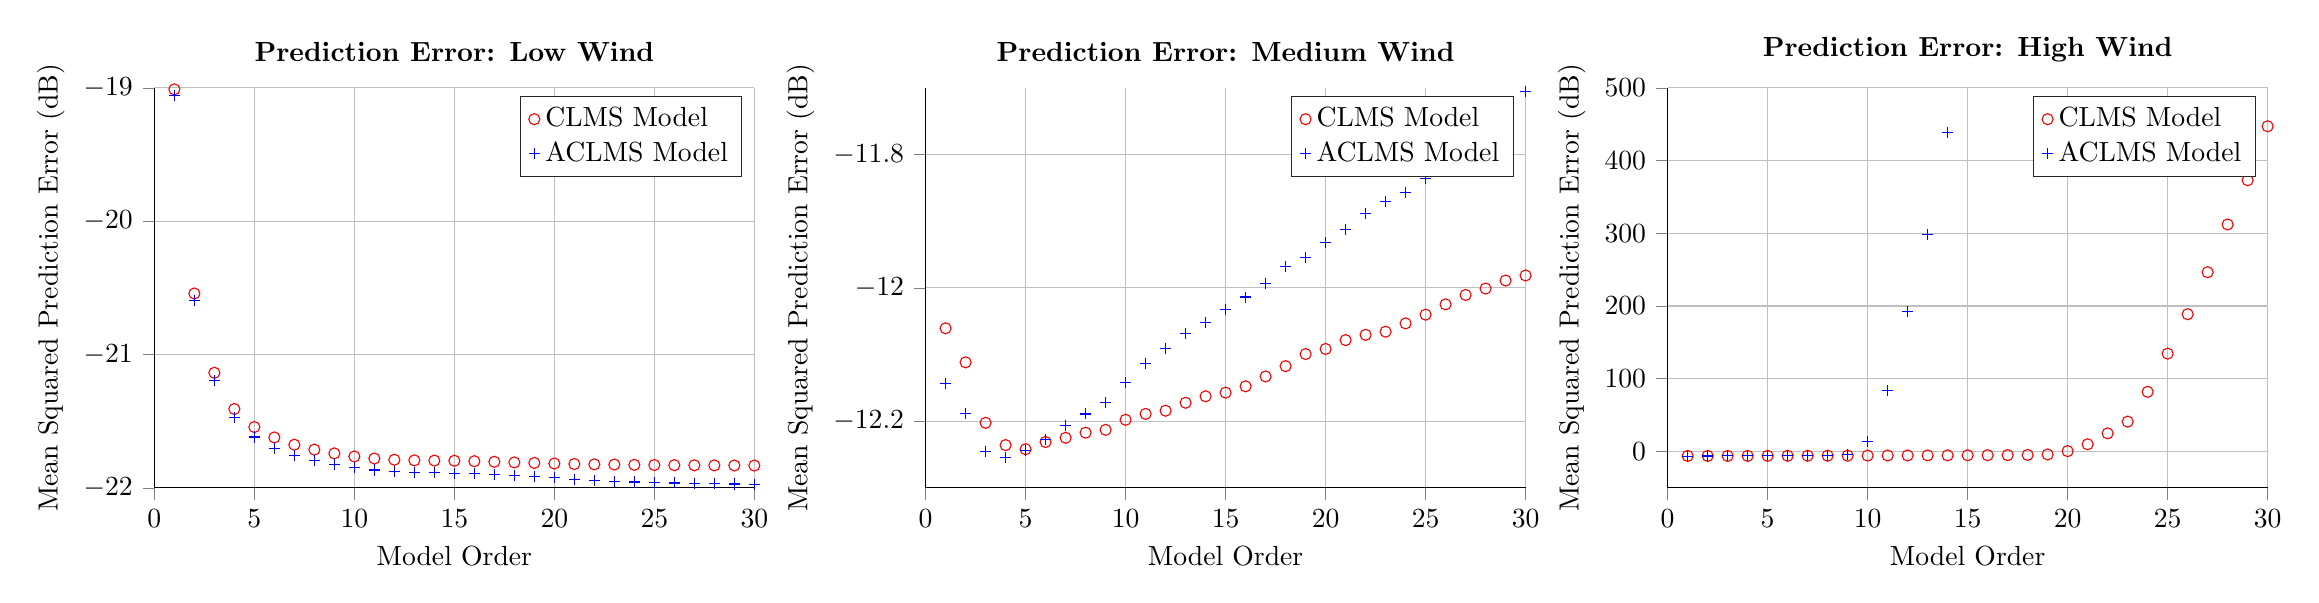
\begin{tikzpicture}


\begin{axis}[%
width=3in,
height=2in,
name=plot2,
scale only axis,
xmin=0,
xmax=30,
tick align=outside,
xlabel={Model Order},
xmajorgrids,
ymin=-12.3,
ymax=-11.7,
ylabel={Mean Squared Prediction Error (dB)},
ymajorgrids,
title style={font=\bfseries},
title={Prediction Error: Medium Wind},
name=plot2,
axis x line*=bottom,
axis y line*=left,
legend style={legend cell align=left,align=left,draw=white!15!black}
]
\addplot [color=red,only marks,mark=o,mark options={solid}]
  table[row sep=crcr]{%
1   -12.0606341141169\\
2   -12.1117457528455\\
3   -12.2024274133328\\
4   -12.2358415398769\\
5   -12.2420129878509\\
6   -12.2312101073906\\
7   -12.2248526872736\\
8   -12.2172082346537\\
9   -12.212980322364\\
10  -12.1978498773172\\
11  -12.1890437031208\\
12  -12.1842568101551\\
13  -12.1723160399597\\
14  -12.1626833400372\\
15  -12.157161539006\\
16  -12.1476901839831\\
17  -12.1328390119391\\
18  -12.1173982872277\\
19  -12.0992597145623\\
20  -12.0916134827479\\
21  -12.0783717856832\\
22  -12.070484214574\\
23  -12.0657062527785\\
24  -12.0532604229908\\
25  -12.0401812370563\\
26  -12.0247029919252\\
27  -12.0106112111109\\
28  -12.0009927546442\\
29  -11.9890074533023\\
30  -11.9813826307998\\
};
\addlegendentry{CLMS Model};

\addplot [color=blue,only marks,mark=+,mark options={solid}]
  table[row sep=crcr]{%
1   -12.1441140092152\\
2   -12.1888616016562\\
3   -12.2460187267115\\
4   -12.2542076548321\\
5   -12.2434272689481\\
6   -12.2270517467743\\
7   -12.2060471550279\\
8   -12.189144029675\\
9   -12.1715687386542\\
10  -12.1418958563171\\
11  -12.1128704098645\\
12  -12.0908897160449\\
13  -12.0683248107994\\
14  -12.051678577953\\
15  -12.0323368723327\\
16  -12.0137607578233\\
17  -11.9929951713869\\
18  -11.9677434821413\\
19  -11.9538427652541\\
20  -11.9321819108073\\
21  -11.9119489249976\\
22  -11.8878656141567\\
23  -11.8705352235024\\
24  -11.8563117898742\\
25  -11.8357531371744\\
26  -11.8144267672742\\
27  -11.7916732627257\\
28  -11.7593837055202\\
29  -11.7292848060645\\
30  -11.7050136472103\\
};
\addlegendentry{ACLMS Model};

\end{axis}

\begin{axis}[%
width=3in,
height=2in,
at=(plot2.right of south east),
anchor=left of south west,
scale only axis,
unbounded coords=jump,
xmin=0,
xmax=30,
tick align=outside,
xlabel={Model Order},
xmajorgrids,
ymin=-50,
ymax=500,
ylabel={Mean Squared Prediction Error (dB)},
ymajorgrids,
title style={font=\bfseries},
title={Prediction Error: High Wind},
axis x line*=bottom,
axis y line*=left,
legend style={legend cell align=left,align=left,draw=white!15!black}
]
\addplot [color=red,only marks,mark=o,mark options={solid}]
  table[row sep=crcr]{%
1	-6.13067897635296\\
2	-6.08348316208382\\
3	-6.07231818854174\\
4	-6.02114771611617\\
5	-5.94628297610506\\
6	-5.87909269058981\\
7	-5.81383714745371\\
8	-5.74985556293042\\
9	-5.69440352513106\\
10	-5.61922042518492\\
11	-5.53835919182432\\
12	-5.45134264471783\\
13	-5.35505956443349\\
14	-5.28367098609307\\
15	-5.18099053224851\\
16	-5.07671322277592\\
17	-4.95831428597084\\
18	-4.67707099938673\\
19	-4.1590592614732\\
20	0.495812298959605\\
21	9.89940263595152\\
22	24.9526805576973\\
23	41.0759244152931\\
24	82.0428518957138\\
25	134.59050983447\\
26	188.808467457773\\
27	246.547665139519\\
28	312.163451333818\\
29	372.99557803487\\
30	447.217699970669\\
};
\addlegendentry{CLMS Model};

\addplot [color=blue,only marks,mark=+,mark options={solid}]
  table[row sep=crcr]{%
1	-6.28578762278148\\
2	-6.17239398858586\\
3	-6.04703132215834\\
4	-5.90212079464262\\
5	-5.74177155815149\\
6	-5.56480537627921\\
7	-5.40029073351247\\
8	-5.07467774438313\\
9	-3.61531889225607\\
10	13.8897956400393\\
11	83.5600562893855\\
12	191.982328909864\\
13	298.470397971174\\
14	438.911589206347\\
15	583.87362821109\\
16	686.014049776815\\
17	899.164550251636\\
18	1088.89100529558\\
19	1296.75702661485\\
20	1565.84253369315\\
21	1767.50092303327\\
22	2032.29075146189\\
23	2280.55385664762\\
24	2646.24750595147\\
25	2998.00383495073\\
26	inf\\
27	inf\\
28	inf\\
29	inf\\
30	inf\\
};
\addlegendentry{ACLMS Model};

\end{axis}


\begin{axis}[%
width=3in,
height=2in,
at=(plot2.left of south west),
anchor=right of south east,
scale only axis,
xmin=0,
xmax=30,
tick align=outside,
xlabel={Model Order},
xmajorgrids,
ymin=-22,
ymax=-19,
ylabel={Mean Squared Prediction Error (dB)},
ymajorgrids,
title style={font=\bfseries},
title={Prediction Error: Low Wind},
axis x line*=bottom,
axis y line*=left,
legend style={legend cell align=left,align=left,draw=white!15!black}
]
\addplot [color=red,only marks,mark=o,mark options={solid}]
  table[row sep=crcr]{%
1	-19.0113369875983\\
2	-20.5420708933905\\
3	-21.1367443291986\\
4	-21.4086270501586\\
5	-21.5438067407019\\
6	-21.6217773528523\\
7	-21.6763524586027\\
8	-21.7132572386021\\
9	-21.7413729669176\\
10	-21.7646338067039\\
11	-21.7798920169207\\
12	-21.78921572449\\
13	-21.7937416549612\\
14	-21.7954497472448\\
15	-21.7964383078291\\
16	-21.8001212491895\\
17	-21.804503562432\\
18	-21.8090513868467\\
19	-21.81269439145\\
20	-21.8173997395156\\
21	-21.8212234382232\\
22	-21.8236033199591\\
23	-21.8251286862162\\
24	-21.8273962866589\\
25	-21.8287563645958\\
26	-21.8299485763325\\
27	-21.8306643969426\\
28	-21.8313822308126\\
29	-21.8320529821532\\
30	-21.8326882570924\\
};
\addlegendentry{CLMS Model};

\addplot [color=blue,only marks,mark=+,mark options={solid}]
  table[row sep=crcr]{%
1	-19.057518964759\\
2	-20.5937220459197\\
3	-21.1925618698586\\
4	-21.4708590805011\\
5	-21.6187491963352\\
6	-21.7023846167023\\
7	-21.7563225089605\\
8	-21.7943665077841\\
9	-21.8248669045148\\
10	-21.8482724983224\\
11	-21.8661305192308\\
12	-21.8767274459613\\
13	-21.8845851969629\\
14	-21.8880848291091\\
15	-21.8897621288285\\
16	-21.8947794372178\\
17	-21.8989862745625\\
18	-21.90746605474\\
19	-21.9143361967006\\
20	-21.9243365758934\\
21	-21.935279677913\\
22	-21.9437258683483\\
23	-21.9491965984726\\
24	-21.9559903669559\\
25	-21.9594109604278\\
26	-21.9631208455449\\
27	-21.966225976195\\
28	-21.9683614570336\\
29	-21.9709194572349\\
30	-21.9730454595313\\
};
\addlegendentry{ACLMS Model};

\end{axis}
\end{tikzpicture}%}
	\caption{\textit{Prediction Error Estimates for varying Model Orders}}
	\label{fig:4_1_b_order}
\end{figure}

\subsubsection{Three Phase Power: Balanced \& Unbalanced Systems} \label{sec:4_1_c}

Using the Clarke Voltage, we can compute $v(n)$ for both a balanced and unbalanced system. Figure \ref{fig:4_1_c} shows the circularity diagram of the complex voltage (both a balanced and unbalanced system). The balanced system has a circular shape to it, whereas the unbalanced system's circularity diagram is more akin to a rugby ball than a circle. The unbalanced nature of the system was demonstated when either a phase shift is introduced in to one or two of the lines, or the voltage across each phase is different. In this case, a phase shift of $\frac{\pi}{8}$ has been applied to one phase, with another having phase shift $-\frac{\pi}{7}$.

\begin{figure}[h]
	\centering
	\resizebox{0.45\textwidth}{!}{% This file was created by matlab2tikz.
% Minimal pgfplots version: 1.3
%
%The latest updates can be retrieved from
%  http://www.mathworks.com/matlabcentral/fileexchange/22022-matlab2tikz
%where you can also make suggestions and rate matlab2tikz.
%
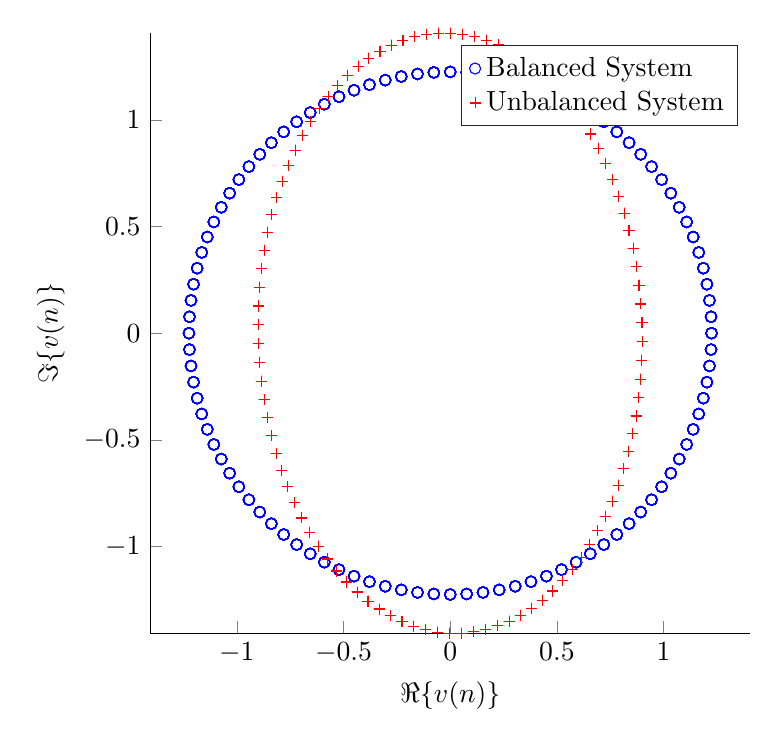
\begin{tikzpicture}

\begin{axis}[%
width=3in,
height=3in,
at={(1.011111in,0.641667in)},
scale only axis,
xmin=-1.40618695186177,
xmax=1.40618695186176,
xlabel={$ \Re \{ v(n) \} $},
ymin=-1.40618695186177,
ymax=1.40618695186176,
ylabel={$ \Im \{ v(n) \} $},
axis x line*=bottom,
axis y line*=left,
legend style={legend cell align=left,align=left,draw=white!15!black}
]
\addplot [color=blue,only marks,mark=o,mark options={solid}]
  table[row sep=crcr]{%
1.22232811715425	0.07690236676554\\
1.2150873922671	0.153501235022806\\
1.20305127256331	0.22949430403348\\
1.18626725910854	0.304581663872109\\
1.16480159073604	0.37846697903356\\
1.13873898263213	0.450858657933882\\
1.10818229200413	0.521471003689067\\
1.07325211214991	0.590025341630131\\
1.03408629653129	0.656251119104719\\
0.990839414729355	0.719886973224818\\
0.94368214242895	0.780681762346672\\
0.89280058783974	0.838395557212116\\
0.838395557212116	0.89280058783974\\
0.780681762346673	0.94368214242895\\
0.719886973224818	0.990839414729355\\
0.656251119104718	1.03408629653129\\
0.590025341630131	1.07325211214991\\
0.521471003689067	1.10818229200413\\
0.450858657933882	1.13873898263213\\
0.37846697903356	1.16480159073604\\
0.304581663872109	1.18626725910854\\
0.22949430403348	1.20305127256331\\
0.153501235022806	1.2150873922671\\
0.0769023667655401	1.22232811715425\\
7.49939943260923e-17	1.22474487139159\\
-0.07690236676554	1.22232811715425\\
-0.153501235022805	1.2150873922671\\
-0.22949430403348	1.20305127256331\\
-0.304581663872109	1.18626725910854\\
-0.37846697903356	1.16480159073604\\
-0.450858657933882	1.13873898263213\\
-0.521471003689067	1.10818229200413\\
-0.590025341630131	1.07325211214991\\
-0.656251119104719	1.03408629653129\\
-0.719886973224818	0.990839414729355\\
-0.780681762346673	0.94368214242895\\
-0.838395557212116	0.89280058783974\\
-0.89280058783974	0.838395557212116\\
-0.94368214242895	0.780681762346673\\
-0.990839414729355	0.719886973224818\\
-1.03408629653129	0.656251119104719\\
-1.07325211214991	0.590025341630131\\
-1.10818229200413	0.521471003689067\\
-1.13873898263213	0.450858657933882\\
-1.16480159073604	0.37846697903356\\
-1.18626725910854	0.304581663872109\\
-1.20305127256331	0.22949430403348\\
-1.2150873922671	0.153501235022806\\
-1.22232811715425	0.0769023667655408\\
-1.22474487139159	1.49987988652185e-16\\
-1.22232811715425	-0.0769023667655394\\
-1.2150873922671	-0.153501235022806\\
-1.20305127256331	-0.22949430403348\\
-1.18626725910854	-0.304581663872108\\
-1.16480159073604	-0.378466979033561\\
-1.13873898263213	-0.450858657933882\\
-1.10818229200413	-0.521471003689066\\
-1.07325211214991	-0.59002534163013\\
-1.03408629653129	-0.656251119104718\\
-0.990839414729355	-0.719886973224818\\
-0.94368214242895	-0.780681762346672\\
-0.89280058783974	-0.838395557212116\\
-0.838395557212116	-0.89280058783974\\
-0.780681762346672	-0.94368214242895\\
-0.719886973224819	-0.990839414729354\\
-0.656251119104718	-1.03408629653129\\
-0.590025341630132	-1.07325211214991\\
-0.521471003689066	-1.10818229200413\\
-0.450858657933883	-1.13873898263213\\
-0.378466979033561	-1.16480159073604\\
-0.304581663872109	-1.18626725910854\\
-0.22949430403348	-1.20305127256331\\
-0.153501235022806	-1.2150873922671\\
-0.0769023667655398	-1.22232811715425\\
-2.24981982978277e-16	-1.22474487139159\\
0.0769023667655393	-1.22232811715425\\
0.153501235022806	-1.2150873922671\\
0.22949430403348	-1.20305127256331\\
0.304581663872109	-1.18626725910854\\
0.37846697903356	-1.16480159073604\\
0.450858657933881	-1.13873898263213\\
0.521471003689067	-1.10818229200413\\
0.590025341630131	-1.07325211214991\\
0.656251119104719	-1.03408629653129\\
0.719886973224817	-0.990839414729355\\
0.780681762346672	-0.943682142428951\\
0.838395557212115	-0.89280058783974\\
0.892800587839739	-0.838395557212117\\
0.94368214242895	-0.780681762346672\\
0.990839414729355	-0.719886973224818\\
1.03408629653129	-0.656251119104719\\
1.07325211214991	-0.590025341630132\\
1.10818229200413	-0.521471003689067\\
1.13873898263213	-0.450858657933882\\
1.16480159073604	-0.37846697903356\\
1.18626725910854	-0.30458166387211\\
1.20305127256331	-0.22949430403348\\
1.2150873922671	-0.153501235022807\\
1.22232811715425	-0.0769023667655387\\
1.22474487139159	-2.99975977304369e-16\\
1.22232811715425	0.0769023667655403\\
1.21508739226711	0.153501235022805\\
1.20305127256331	0.22949430403348\\
1.18626725910854	0.304581663872109\\
1.16480159073604	0.37846697903356\\
1.13873898263213	0.450858657933882\\
1.10818229200413	0.521471003689067\\
1.07325211214991	0.590025341630129\\
1.03408629653129	0.656251119104719\\
0.990839414729354	0.719886973224818\\
0.943682142428951	0.780681762346672\\
0.892800587839741	0.838395557212115\\
0.838395557212117	0.892800587839739\\
0.780681762346673	0.943682142428949\\
0.719886973224818	0.990839414729355\\
0.656251119104719	1.03408629653129\\
0.590025341630131	1.07325211214991\\
0.521471003689067	1.10818229200413\\
0.450858657933883	1.13873898263213\\
0.378466979033561	1.16480159073604\\
0.304581663872109	1.18626725910854\\
0.22949430403348	1.20305127256331\\
0.153501235022807	1.2150873922671\\
0.0769023667655399	1.22232811715425\\
1.46276193603888e-15	1.22474487139159\\
-0.0769023667655402	1.22232811715425\\
-0.153501235022805	1.21508739226711\\
-0.229494304033481	1.20305127256331\\
-0.304581663872109	1.18626725910854\\
-0.378466979033558	1.16480159073604\\
-0.450858657933881	1.13873898263213\\
-0.521471003689068	1.10818229200413\\
-0.590025341630131	1.07325211214991\\
-0.656251119104717	1.03408629653129\\
-0.719886973224817	0.990839414729355\\
-0.780681762346674	0.943682142428949\\
-0.838395557212115	0.892800587839741\\
-0.892800587839739	0.838395557212118\\
-0.94368214242895	0.780681762346673\\
-0.990839414729355	0.719886973224818\\
-1.03408629653129	0.656251119104719\\
-1.07325211214991	0.590025341630132\\
-1.10818229200413	0.521471003689066\\
-1.13873898263213	0.450858657933882\\
-1.16480159073604	0.378466979033561\\
-1.18626725910854	0.30458166387211\\
-1.20305127256331	0.229494304033479\\
-1.2150873922671	0.153501235022805\\
-1.22232811715425	0.0769023667655422\\
-1.22474487139159	4.49963965956554e-16\\
-1.22232811715425	-0.0769023667655391\\
-1.21508739226711	-0.153501235022804\\
-1.20305127256331	-0.229494304033478\\
-1.18626725910854	-0.304581663872109\\
-1.16480159073604	-0.37846697903356\\
-1.13873898263213	-0.450858657933881\\
-1.10818229200413	-0.521471003689066\\
-1.07325211214991	-0.590025341630131\\
-1.03408629653129	-0.656251119104718\\
-0.990839414729355	-0.719886973224817\\
-0.943682142428951	-0.780681762346672\\
-0.892800587839741	-0.838395557212115\\
-0.838395557212118	-0.892800587839739\\
-0.780681762346673	-0.94368214242895\\
-0.71988697322482	-0.990839414729353\\
-0.656251119104717	-1.03408629653129\\
-0.59002534163013	-1.07325211214991\\
-0.521471003689066	-1.10818229200413\\
-0.450858657933882	-1.13873898263213\\
-0.378466979033561	-1.16480159073604\\
-0.30458166387211	-1.18626725910854\\
-0.229494304033482	-1.20305127256331\\
-0.153501235022808	-1.2150873922671\\
-0.0769023667655422	-1.22232811715425\\
-5.24957960282646e-16	-1.22474487139159\\
0.076902366765539	-1.22232811715425\\
0.153501235022807	-1.2150873922671\\
0.229494304033481	-1.20305127256331\\
0.304581663872109	-1.18626725910854\\
0.37846697903356	-1.16480159073604\\
0.450858657933881	-1.13873898263213\\
0.521471003689066	-1.10818229200413\\
0.590025341630131	-1.07325211214991\\
0.656251119104717	-1.03408629653129\\
0.719886973224816	-0.990839414729356\\
0.780681762346672	-0.943682142428951\\
0.838395557212117	-0.892800587839739\\
0.89280058783974	-0.838395557212116\\
0.94368214242895	-0.780681762346673\\
0.990839414729356	-0.719886973224816\\
1.03408629653129	-0.656251119104719\\
1.07325211214991	-0.590025341630132\\
1.10818229200412	-0.521471003689069\\
1.13873898263213	-0.450858657933882\\
1.16480159073604	-0.378466979033561\\
1.18626725910854	-0.304581663872112\\
1.20305127256331	-0.229494304033482\\
1.21508739226711	-0.153501235022803\\
1.22232811715425	-0.0769023667655401\\
1.22474487139159	-5.99951954608738e-16\\
1.22232811715425	0.0769023667655389\\
1.2150873922671	0.153501235022806\\
1.20305127256331	0.229494304033478\\
1.18626725910854	0.304581663872107\\
1.16480159073604	0.37846697903356\\
1.13873898263213	0.450858657933881\\
1.10818229200413	0.521471003689065\\
1.07325211214991	0.590025341630131\\
1.03408629653129	0.656251119104718\\
0.990839414729355	0.719886973224817\\
0.943682142428949	0.780681762346673\\
0.892800587839739	0.838395557212117\\
0.838395557212116	0.89280058783974\\
0.780681762346673	0.94368214242895\\
0.71988697322482	0.990839414729353\\
0.656251119104721	1.03408629653129\\
0.59002534163013	1.07325211214991\\
0.521471003689067	1.10818229200413\\
0.45085865793388	1.13873898263213\\
0.378466979033559	1.16480159073604\\
0.304581663872108	1.18626725910854\\
0.229494304033482	1.20305127256331\\
0.153501235022808	1.2150873922671\\
0.0769023667655424	1.22232811715425\\
-1.500637979882e-15	1.22474487139159\\
-0.0769023667655389	1.22232811715425\\
-0.153501235022804	1.21508739226711\\
-0.229494304033478	1.20305127256331\\
-0.304581663872107	1.18626725910854\\
-0.37846697903356	1.16480159073604\\
-0.450858657933881	1.13873898263213\\
-0.521471003689065	1.10818229200413\\
-0.590025341630131	1.07325211214991\\
-0.656251119104718	1.03408629653129\\
-0.719886973224817	0.990839414729355\\
-0.780681762346672	0.943682142428951\\
-0.838395557212115	0.892800587839741\\
-0.892800587839738	0.838395557212118\\
-0.94368214242895	0.780681762346673\\
-0.990839414729354	0.719886973224818\\
-1.03408629653129	0.656251119104718\\
-1.07325211214991	0.59002534163013\\
-1.10818229200413	0.521471003689067\\
-1.13873898263213	0.450858657933882\\
-1.16480159073604	0.378466979033561\\
-1.18626725910854	0.304581663872112\\
-1.20305127256331	0.22949430403348\\
-1.2150873922671	0.153501235022806\\
-1.22232811715425	0.0769023667655403\\
-1.22474487139159	2.92552387207775e-15\\
-1.22232811715425	-0.0769023667655409\\
-1.2150873922671	-0.153501235022806\\
-1.20305127256331	-0.229494304033478\\
-1.18626725910854	-0.304581663872106\\
-1.16480159073604	-0.378466979033562\\
-1.13873898263213	-0.450858657933883\\
-1.10818229200413	-0.521471003689067\\
-1.07325211214991	-0.590025341630131\\
-1.03408629653129	-0.656251119104718\\
-0.990839414729358	-0.719886973224813\\
-0.943682142428951	-0.780681762346672\\
-0.892800587839741	-0.838395557212115\\
-0.838395557212115	-0.892800587839741\\
-0.780681762346671	-0.943682142428951\\
-0.719886973224817	-0.990839414729356\\
-0.656251119104718	-1.03408629653129\\
-0.590025341630134	-1.07325211214991\\
-0.521471003689071	-1.10818229200412\\
-0.450858657933882	-1.13873898263213\\
-0.378466979033561	-1.16480159073604\\
-0.30458166387211	-1.18626725910854\\
-0.229494304033478	-1.20305127256331\\
-0.153501235022804	-1.21508739226711\\
-0.0769023667655425	-1.22232811715425\\
-3.00051786640384e-15	-1.22474487139159\\
0.0769023667655365	-1.22232811715425\\
0.153501235022806	-1.2150873922671\\
0.22949430403348	-1.20305127256331\\
0.304581663872108	-1.18626725910854\\
0.37846697903356	-1.16480159073604\\
0.450858657933881	-1.13873898263213\\
0.521471003689065	-1.10818229200413\\
0.590025341630129	-1.07325211214991\\
0.656251119104716	-1.03408629653129\\
0.719886973224819	-0.990839414729354\\
0.780681762346673	-0.94368214242895\\
0.838395557212117	-0.89280058783974\\
0.89280058783974	-0.838395557212116\\
0.94368214242895	-0.780681762346673\\
0.990839414729354	-0.719886973224818\\
1.03408629653129	-0.65625111910472\\
1.07325211214991	-0.590025341630132\\
1.10818229200412	-0.521471003689069\\
1.13873898263213	-0.450858657933881\\
1.16480159073604	-0.378466979033559\\
1.18626725910854	-0.304581663872108\\
1.20305127256331	-0.22949430403348\\
1.2150873922671	-0.15350123502281\\
1.22232811715425	-0.0769023667655404\\
1.22474487139159	-8.99927931913108e-16\\
1.22232811715425	0.0769023667655386\\
1.21508739226711	0.153501235022804\\
1.20305127256331	0.229494304033478\\
1.18626725910854	0.304581663872106\\
1.16480159073604	0.378466979033562\\
1.13873898263213	0.450858657933879\\
1.10818229200413	0.521471003689067\\
1.07325211214991	0.590025341630131\\
1.03408629653129	0.656251119104718\\
0.990839414729355	0.719886973224817\\
0.943682142428951	0.780681762346671\\
0.892800587839741	0.838395557212115\\
0.838395557212118	0.892800587839738\\
0.780681762346675	0.943682142428948\\
0.719886973224817	0.990839414729356\\
0.656251119104718	1.03408629653129\\
0.59002534163013	1.07325211214991\\
0.521471003689067	1.10818229200413\\
0.450858657933883	1.13873898263213\\
0.378466979033561	1.16480159073604\\
0.30458166387211	1.18626725910854\\
0.229494304033482	1.2030512725633\\
0.153501235022808	1.2150873922671\\
0.0769023667655427	1.22232811715425\\
3.15050585505603e-15	1.22474487139159\\
-0.0769023667655364	1.22232811715425\\
-0.153501235022806	1.2150873922671\\
-0.22949430403348	1.20305127256331\\
-0.304581663872108	1.18626725910854\\
-0.378466979033555	1.16480159073604\\
-0.450858657933881	1.13873898263213\\
-0.521471003689069	1.10818229200412\\
-0.590025341630129	1.07325211214991\\
-0.65625111910472	1.03408629653129\\
-0.719886973224819	0.990839414729354\\
-0.780681762346673	0.94368214242895\\
-0.838395557212113	0.892800587839742\\
-0.89280058783974	0.838395557212116\\
-0.943682142428947	0.780681762346676\\
-0.990839414729354	0.719886973224819\\
-1.03408629653129	0.656251119104723\\
-1.07325211214991	0.590025341630132\\
-1.10818229200413	0.521471003689065\\
-1.13873898263213	0.450858657933885\\
-1.16480159073604	0.378466979033559\\
-1.18626725910854	0.304581663872112\\
-1.20305127256331	0.22949430403348\\
-1.2150873922671	0.15350123502281\\
-1.22232811715425	0.0769023667655406\\
-1.22474487139159	1.04991592056529e-15\\
-1.22232811715425	-0.0769023667655385\\
-1.21508739226711	-0.153501235022804\\
-1.20305127256331	-0.229494304033478\\
-1.18626725910854	-0.30458166387211\\
-1.16480159073604	-0.378466979033557\\
-1.13873898263213	-0.450858657933883\\
-1.10818229200413	-0.521471003689067\\
-1.07325211214991	-0.590025341630131\\
-1.03408629653129	-0.656251119104718\\
-0.990839414729355	-0.719886973224817\\
-0.943682142428954	-0.780681762346668\\
-0.892800587839741	-0.838395557212115\\
-0.838395557212115	-0.892800587839741\\
-0.780681762346675	-0.943682142428948\\
-0.719886973224817	-0.990839414729355\\
-0.656251119104718	-1.03408629653129\\
-0.590025341630131	-1.07325211214991\\
-0.521471003689071	-1.10818229200412\\
-0.450858657933883	-1.13873898263213\\
-0.378466979033566	-1.16480159073604\\
-0.30458166387211	-1.18626725910854\\
-0.229494304033482	-1.2030512725633\\
-0.153501235022804	-1.21508739226711\\
-0.0769023667655385	-1.22232811715425\\
-3.30049384370821e-15	-1.22474487139159\\
0.0769023667655406	-1.22232811715425\\
0.153501235022802	-1.21508739226711\\
0.22949430403348	-1.20305127256331\\
0.304581663872108	-1.18626725910854\\
0.378466979033563	-1.16480159073604\\
0.450858657933881	-1.13873898263213\\
0.521471003689065	-1.10818229200413\\
0.590025341630129	-1.07325211214991\\
0.656251119104716	-1.03408629653129\\
0.719886973224819	-0.990839414729354\\
0.78068176234667	-0.943682142428953\\
0.838395557212116	-0.89280058783974\\
0.89280058783974	-0.838395557212116\\
0.94368214242895	-0.780681762346673\\
0.990839414729354	-0.719886973224819\\
1.03408629653129	-0.65625111910472\\
1.07325211214991	-0.590025341630136\\
1.10818229200412	-0.521471003689069\\
1.13873898263213	-0.450858657933885\\
1.16480159073604	-0.378466979033559\\
1.18626725910855	-0.304581663872104\\
1.20305127256331	-0.22949430403348\\
1.2150873922671	-0.153501235022806\\
1.22232811715425	-0.0769023667655451\\
1.22474487139159	-1.19990390921748e-15\\
1.22232811715425	0.0769023667655383\\
1.21508739226711	0.153501235022804\\
1.20305127256331	0.229494304033478\\
1.18626725910854	0.30458166387211\\
1.16480159073604	0.378466979033557\\
1.13873898263213	0.450858657933879\\
1.10818229200413	0.521471003689067\\
1.07325211214991	0.590025341630127\\
1.03408629653129	0.656251119104718\\
0.990839414729356	0.719886973224817\\
0.943682142428948	0.780681762346675\\
0.892800587839741	0.838395557212115\\
0.838395557212118	0.892800587839738\\
0.780681762346675	0.943682142428948\\
0.71988697322482	0.990839414729353\\
0.656251119104718	1.03408629653129\\
0.590025341630131	1.07325211214991\\
0.521471003689067	1.10818229200413\\
0.450858657933887	1.13873898263213\\
0.378466979033562	1.16480159073604\\
0.30458166387211	1.18626725910854\\
0.229494304033478	1.20305127256331\\
0.153501235022808	1.2150873922671\\
0.0769023667655386	1.22232811715425\\
3.4504818323604e-15	1.22474487139159\\
-0.0769023667655404	1.22232811715425\\
-0.15350123502281	1.2150873922671\\
-0.22949430403348	1.20305127256331\\
-0.304581663872108	1.18626725910854\\
-0.378466979033555	1.16480159073604\\
-0.450858657933881	1.13873898263213\\
-0.521471003689061	1.10818229200413\\
-0.590025341630128	1.07325211214991\\
-0.65625111910472	1.03408629653129\\
-0.719886973224815	0.990839414729357\\
-0.780681762346673	0.94368214242895\\
-0.838395557212116	0.89280058783974\\
-0.892800587839742	0.838395557212113\\
-0.94368214242895	0.780681762346673\\
-0.990839414729357	0.719886973224815\\
-1.03408629653129	0.65625111910472\\
-1.07325211214991	0.590025341630129\\
-1.10818229200412	0.521471003689069\\
-1.13873898263213	0.450858657933885\\
-1.16480159073604	0.378466979033564\\
-1.18626725910854	0.304581663872113\\
-1.2030512725633	0.229494304033489\\
-1.2150873922671	0.153501235022811\\
-1.22232811715425	0.0769023667655409\\
-1.22474487139159	-3.001275959764e-15\\
-1.22232811715425	-0.0769023667655425\\
-1.21508739226711	-0.153501235022804\\
-1.2030512725633	-0.229494304033482\\
-1.18626725910854	-0.304581663872106\\
-1.16480159073604	-0.378466979033561\\
-1.13873898263213	-0.450858657933878\\
-1.10818229200413	-0.521471003689067\\
-1.07325211214991	-0.590025341630126\\
-1.03408629653129	-0.656251119104718\\
-0.990839414729356	-0.719886973224817\\
-0.943682142428954	-0.780681762346668\\
-0.892800587839741	-0.838395557212115\\
-0.838395557212121	-0.892800587839735\\
-0.780681762346675	-0.943682142428948\\
-0.719886973224817	-0.990839414729355\\
-0.656251119104718	-1.03408629653129\\
-0.590025341630131	-1.07325211214991\\
-0.521471003689067	-1.10818229200413\\
-0.450858657933887	-1.13873898263213\\
-0.378466979033562	-1.16480159073604\\
-0.304581663872106	-1.18626725910854\\
-0.229494304033482	-1.2030512725633\\
-0.153501235022804	-1.21508739226711\\
-0.0769023667655431	-1.22232811715425\\
-3.60046982101258e-15	-1.22474487139159\\
0.0769023667655359	-1.22232811715425\\
0.153501235022801	-1.21508739226711\\
0.22949430403348	-1.20305127256331\\
0.304581663872112	-1.18626725910854\\
0.378466979033559	-1.16480159073604\\
0.450858657933884	-1.13873898263213\\
0.521471003689069	-1.10818229200412\\
0.590025341630128	-1.07325211214991\\
0.65625111910472	-1.03408629653129\\
0.719886973224815	-0.990839414729357\\
0.780681762346673	-0.94368214242895\\
0.838395557212113	-0.892800587839743\\
0.892800587839739	-0.838395557212117\\
0.943682142428947	-0.780681762346677\\
0.990839414729354	-0.719886973224819\\
1.03408629653129	-0.65625111910472\\
1.07325211214991	-0.590025341630137\\
1.10818229200412	-0.521471003689069\\
1.13873898263213	-0.450858657933881\\
1.16480159073604	-0.378466979033556\\
1.18626725910854	-0.304581663872109\\
1.20305127256331	-0.22949430403348\\
1.2150873922671	-0.153501235022806\\
1.22232811715425	-0.076902366765541\\
1.22474487139159	-5.8510477441555e-15\\
1.22232811715425	0.076902366765538\\
1.2150873922671	0.153501235022808\\
1.20305127256331	0.229494304033477\\
1.18626725910854	0.30458166387211\\
1.16480159073604	0.378466979033557\\
1.13873898263213	0.450858657933878\\
1.10818229200413	0.521471003689063\\
1.07325211214991	0.590025341630126\\
1.03408629653129	0.656251119104718\\
0.990839414729353	0.71988697322482\\
0.943682142428951	0.780681762346671\\
0.892800587839738	0.838395557212118\\
0.838395557212112	0.892800587839744\\
0.780681762346672	0.943682142428951\\
0.719886973224814	0.990839414729358\\
0.656251119104718	1.03408629653129\\
0.590025341630135	1.07325211214991\\
0.521471003689067	1.10818229200413\\
0.450858657933887	1.13873898263213\\
0.37846697903357	1.16480159073604\\
0.304581663872115	1.18626725910854\\
0.229494304033483	1.2030512725633\\
0.153501235022813	1.2150873922671\\
0.0769023667655433	1.22232811715425\\
-6.00710047968891e-16	1.22474487139159\\
-0.0769023667655445	1.22232811715425\\
-0.153501235022806	1.2150873922671\\
-0.229494304033484	1.2030512725633\\
-0.304581663872108	1.18626725910854\\
-0.378466979033563	1.16480159073604\\
-0.45085865793388	1.13873898263213\\
-0.521471003689069	1.10818229200412\\
-0.590025341630128	1.07325211214991\\
-0.656251119104712	1.0340862965313\\
-0.719886973224815	0.990839414729357\\
-0.780681762346666	0.943682142428956\\
-0.838395557212113	0.892800587839743\\
-0.892800587839739	0.838395557212117\\
-0.943682142428952	0.78068176234667\\
-0.990839414729354	0.719886973224819\\
-1.03408629653129	0.656251119104717\\
-1.07325211214991	0.590025341630133\\
-1.10818229200413	0.521471003689066\\
-1.13873898263213	0.450858657933877\\
-1.16480159073604	0.37846697903356\\
-1.18626725910855	0.304581663872105\\
-1.20305127256331	0.229494304033481\\
-1.2150873922671	0.153501235022811\\
-1.22232811715425	0.0769023667655412\\
-1.22474487139159	6.00103573280769e-15\\
-1.22232811715425	-0.0769023667655292\\
-1.21508739226711	-0.153501235022799\\
-1.20305127256331	-0.229494304033477\\
-1.18626725910854	-0.30458166387211\\
-1.16480159073604	-0.378466979033565\\
-1.13873898263213	-0.450858657933882\\
-1.10818229200412	-0.52147100368907\\
-1.07325211214991	-0.59002534163013\\
-1.03408629653129	-0.656251119104721\\
-0.990839414729356	-0.719886973224816\\
-0.943682142428949	-0.780681762346674\\
-0.892800587839741	-0.838395557212114\\
-0.838395557212115	-0.892800587839741\\
-0.780681762346675	-0.943682142428948\\
-0.719886973224824	-0.99083941472935\\
-0.656251119104722	-1.03408629653129\\
-0.590025341630131	-1.07325211214991\\
-0.521471003689072	-1.10818229200412\\
-0.450858657933883	-1.13873898263213\\
-0.378466979033558	-1.16480159073604\\
-0.304581663872111	-1.18626725910854\\
-0.229494304033478	-1.20305127256331\\
-0.153501235022809	-1.2150873922671\\
-0.0769023667655391	-1.22232811715425\\
-3.90044579831695e-15	-1.22474487139159\\
0.07690236676554	-1.22232811715425\\
0.15350123502281	-1.2150873922671\\
0.229494304033479	-1.20305127256331\\
0.304581663872112	-1.18626725910854\\
0.378466979033559	-1.16480159073604\\
0.450858657933876	-1.13873898263213\\
0.521471003689064	-1.10818229200413\\
0.590025341630132	-1.07325211214991\\
0.656251119104716	-1.03408629653129\\
0.719886973224818	-0.990839414729355\\
0.780681762346669	-0.943682142428953\\
0.838395557212116	-0.89280058783974\\
0.892800587839742	-0.838395557212114\\
0.943682142428949	-0.780681762346674\\
0.990839414729356	-0.719886973224816\\
1.03408629653129	-0.65625111910472\\
1.07325211214991	-0.590025341630129\\
1.10818229200412	-0.52147100368907\\
1.13873898263213	-0.450858657933881\\
1.16480159073604	-0.378466979033564\\
1.18626725910854	-0.304581663872117\\
1.2030512725633	-0.229494304033485\\
1.2150873922671	-0.153501235022807\\
1.22232811715425	-0.076902366765537\\
1.22474487139159	-1.79985586382622e-15\\
1.22232811715425	0.0769023667655421\\
1.21508739226711	0.153501235022803\\
1.20305127256331	0.229494304033481\\
1.18626725910854	0.304581663872105\\
1.16480159073604	0.378466979033561\\
1.13873898263213	0.450858657933878\\
1.10818229200413	0.521471003689066\\
1.07325211214991	0.590025341630126\\
1.03408629653129	0.656251119104717\\
0.990839414729353	0.71988697322482\\
0.943682142428952	0.780681762346671\\
0.892800587839745	0.838395557212111\\
0.838395557212118	0.892800587839738\\
0.780681762346672	0.943682142428951\\
0.719886973224821	0.990839414729352\\
0.656251119104719	1.03408629653129\\
0.590025341630135	1.07325211214991\\
0.521471003689068	1.10818229200413\\
0.450858657933879	1.13873898263213\\
0.378466979033562	1.16480159073604\\
0.304581663872107	1.18626725910854\\
0.229494304033483	1.2030512725633\\
0.153501235022805	1.21508739226711\\
0.0769023667655436	1.22232811715425\\
-3.00734070664522e-16	1.22474487139159\\
-0.0769023667655355	1.22232811715425\\
-0.153501235022805	1.2150873922671\\
-0.229494304033475	1.20305127256331\\
-0.304581663872107	1.18626725910854\\
-0.378466979033563	1.16480159073604\\
-0.45085865793388	1.13873898263213\\
-0.521471003689068	1.10818229200412\\
-0.590025341630128	1.07325211214991\\
-0.656251119104719	1.03408629653129\\
-0.719886973224814	0.990839414729357\\
-0.780681762346672	0.94368214242895\\
-0.838395557212113	0.892800587839743\\
-0.892800587839739	0.838395557212117\\
-0.943682142428946	0.780681762346677\\
-0.990839414729354	0.719886973224819\\
-1.03408629653129	0.656251119104717\\
-1.07325211214991	0.590025341630133\\
-1.10818229200413	0.521471003689066\\
-1.13873898263213	0.450858657933886\\
-1.16480159073604	0.37846697903356\\
-1.18626725910854	0.304581663872113\\
-1.20305127256331	0.229494304033481\\
-1.2150873922671	0.153501235022811\\
-1.22232811715425	0.0769023667655415\\
-1.22474487139159	6.30101171011206e-15\\
-1.22232811715425	-0.0769023667655376\\
-1.21508739226711	-0.153501235022799\\
-1.2030512725633	-0.229494304033486\\
-1.18626725910854	-0.304581663872109\\
-1.16480159073604	-0.378466979033565\\
-1.13873898263213	-0.450858657933882\\
-1.10818229200413	-0.521471003689062\\
-1.07325211214991	-0.59002534163013\\
-1.0340862965313	-0.656251119104714\\
-0.990839414729361	-0.719886973224809\\
-0.943682142428949	-0.780681762346674\\
-0.892800587839742	-0.838395557212114\\
-0.838395557212122	-0.892800587839734\\
-0.780681762346669	-0.943682142428953\\
-0.719886973224818	-0.990839414729355\\
-0.656251119104722	-1.03408629653129\\
-0.590025341630139	-1.07325211214991\\
-0.521471003689064	-1.10818229200413\\
-0.450858657933884	-1.13873898263213\\
-0.378466979033558	-1.16480159073604\\
-0.304581663872111	-1.18626725910854\\
-0.229494304033479	-1.20305127256331\\
-0.153501235022809	-1.2150873922671\\
-0.0769023667655481	-1.22232811715425\\
4.501913939646e-15	-1.22474487139159\\
0.0769023667655397	-1.22232811715425\\
0.153501235022801	-1.21508739226711\\
0.22949430403347	-1.20305127256331\\
0.304581663872111	-1.18626725910854\\
0.378466979033558	-1.16480159073604\\
0.450858657933876	-1.13873898263213\\
0.521471003689056	-1.10818229200413\\
0.590025341630132	-1.07325211214991\\
0.656251119104715	-1.03408629653129\\
0.719886973224818	-0.990839414729355\\
0.780681762346676	-0.943682142428948\\
0.838395557212116	-0.89280058783974\\
0.892800587839736	-0.83839555721212\\
0.943682142428943	-0.78068176234668\\
0.990839414729356	-0.719886973224816\\
1.03408629653129	-0.656251119104721\\
1.07325211214991	-0.590025341630137\\
1.10818229200412	-0.521471003689078\\
1.13873898263213	-0.450858657933882\\
1.16480159073604	-0.378466979033564\\
1.18626725910854	-0.304581663872118\\
1.20305127256331	-0.229494304033477\\
1.2150873922671	-0.153501235022807\\
1.22232811715425	-0.076902366765546\\
1.22474487139159	-2.09983184113058e-15\\
1.22232811715425	0.0769023667655418\\
1.21508739226711	0.153501235022803\\
1.20305127256331	0.229494304033481\\
1.18626725910854	0.304581663872105\\
1.16480159073604	0.37846697903356\\
1.13873898263213	0.450858657933878\\
1.10818229200413	0.521471003689058\\
1.07325211214991	0.590025341630133\\
1.03408629653129	0.656251119104717\\
0.990839414729359	0.719886973224812\\
0.943682142428957	0.780681762346664\\
0.892800587839739	0.838395557212117\\
0.838395557212119	0.892800587839737\\
0.780681762346672	0.94368214242895\\
0.719886973224814	0.990839414729357\\
0.656251119104719	1.03408629653129\\
0.590025341630128	1.07325211214991\\
0.521471003689068	1.10818229200413\\
0.45085865793388	1.13873898263213\\
0.378466979033562	1.16480159073604\\
0.304581663872116	1.18626725910854\\
0.229494304033492	1.2030512725633\\
0.153501235022805	1.2150873922671\\
0.0769023667655439	1.22232811715425\\
8.70157762190716e-15	1.22474487139159\\
-0.0769023667655439	1.22232811715425\\
-0.153501235022805	1.2150873922671\\
-0.229494304033475	1.20305127256331\\
-0.304581663872107	1.18626725910854\\
-0.378466979033562	1.16480159073604\\
-0.450858657933888	1.13873898263213\\
-0.521471003689068	1.10818229200413\\
-0.590025341630128	1.07325211214991\\
-0.656251119104719	1.03408629653129\\
-0.719886973224814	0.990839414729357\\
-0.780681762346665	0.943682142428956\\
-0.838395557212119	0.892800587839737\\
-0.892800587839739	0.838395557212117\\
-0.943682142428946	0.780681762346677\\
-0.990839414729348	0.719886973224827\\
-1.03408629653129	0.656251119104717\\
-1.07325211214991	0.590025341630133\\
-1.10818229200413	0.521471003689066\\
-1.13873898263213	0.450858657933886\\
-1.16480159073604	0.37846697903356\\
-1.18626725910854	0.304581663872105\\
-1.20305127256331	0.229494304033481\\
-1.21508739226711	0.153501235022803\\
-1.22232811715425	0.0769023667655418\\
-1.22474487139159	6.60098768741643e-15\\
-1.22232811715425	-0.0769023667655286\\
-1.2150873922671	-0.153501235022807\\
-1.20305127256331	-0.229494304033477\\
-1.18626725910855	-0.304581663872101\\
-1.16480159073604	-0.378466979033548\\
-1.13873898263213	-0.450858657933882\\
-1.10818229200413	-0.521471003689062\\
-1.07325211214991	-0.59002534163013\\
-1.03408629653129	-0.656251119104721\\
-0.990839414729351	-0.719886973224823\\
-0.943682142428949	-0.780681762346674\\
-0.892800587839742	-0.838395557212114\\
-0.838395557212116	-0.89280058783974\\
-0.780681762346676	-0.943682142428948\\
-0.719886973224818	-0.990839414729355\\
-0.656251119104723	-1.03408629653129\\
-0.590025341630132	-1.07325211214991\\
-0.521471003689072	-1.10818229200412\\
-0.450858657933892	-1.13873898263213\\
-0.378466979033558	-1.16480159073604\\
-0.304581663872111	-1.18626725910854\\
-0.229494304033488	-1.2030512725633\\
-0.153501235022809	-1.2150873922671\\
-0.0769023667655397	-1.22232811715425\\
4.20193796234163e-15	-1.22474487139159\\
0.0769023667655394	-1.22232811715425\\
0.1535012350228	-1.21508739226711\\
0.229494304033479	-1.20305127256331\\
0.304581663872111	-1.18626725910854\\
0.378466979033558	-1.16480159073604\\
0.450858657933884	-1.13873898263213\\
0.521471003689064	-1.10818229200413\\
0.590025341630124	-1.07325211214992\\
0.656251119104708	-1.0340862965313\\
0.719886973224818	-0.990839414729355\\
0.780681762346669	-0.943682142428953\\
0.838395557212109	-0.892800587839746\\
0.892800587839736	-0.83839555721212\\
0.943682142428949	-0.780681762346674\\
0.990839414729356	-0.719886973224816\\
1.03408629653129	-0.656251119104721\\
1.07325211214992	-0.590025341630122\\
1.10818229200413	-0.521471003689062\\
1.13873898263213	-0.450858657933882\\
1.16480159073604	-0.378466979033565\\
1.18626725910854	-0.304581663872109\\
1.2030512725633	-0.229494304033486\\
1.2150873922671	-0.153501235022816\\
1.22232811715425	-0.076902366765555\\
1.22474487139159	-2.39980781843495e-15\\
1.22232811715425	0.0769023667655328\\
1.21508739226711	0.153501235022803\\
1.20305127256331	0.229494304033481\\
1.18626725910855	0.304581663872105\\
1.16480159073604	0.37846697903356\\
1.13873898263213	0.450858657933877\\
1.10818229200412	0.521471003689074\\
1.07325211214991	0.590025341630133\\
1.03408629653129	0.656251119104717\\
0.990839414729359	0.719886973224812\\
0.943682142428952	0.78068176234667\\
0.892800587839745	0.838395557212111\\
0.838395557212119	0.892800587839737\\
0.780681762346672	0.94368214242895\\
0.719886973224821	0.990839414729352\\
0.656251119104726	1.03408629653129\\
0.590025341630136	1.07325211214991\\
0.521471003689068	1.10818229200412\\
0.45085865793388	1.13873898263213\\
0.378466979033563	1.16480159073604\\
0.304581663872116	1.18626725910854\\
0.229494304033475	1.20305127256331\\
0.153501235022805	1.2150873922671\\
0.0769023667655442	1.22232811715425\\
2.99217883944217e-16	1.22474487139159\\
-0.0769023667655349	1.22232811715425\\
-0.153501235022805	1.21508739226711\\
-0.229494304033474	1.20305127256331\\
-0.304581663872107	1.18626725910854\\
-0.378466979033554	1.16480159073604\\
-0.450858657933879	1.13873898263213\\
-0.521471003689068	1.10818229200413\\
-0.590025341630127	1.07325211214991\\
-0.656251119104719	1.03408629653129\\
-0.719886973224814	0.990839414729358\\
-0.780681762346672	0.943682142428951\\
-0.838395557212118	0.892800587839738\\
-0.892800587839733	0.838395557212124\\
-0.943682142428946	0.780681762346677\\
-0.990839414729353	0.71988697322482\\
-1.03408629653129	0.656251119104717\\
-1.07325211214991	0.590025341630134\\
-1.10818229200413	0.521471003689066\\
-1.13873898263213	0.450858657933878\\
-1.16480159073604	0.378466979033569\\
-1.18626725910854	0.304581663872114\\
-1.20305127256331	0.229494304033481\\
-1.21508739226711	0.153501235022803\\
-1.22232811715425	0.0769023667655508\\
-1.22474487139159	6.9009636647208e-15\\
-1.22232811715425	-0.076902366765537\\
-1.2150873922671	-0.153501235022807\\
-1.20305127256331	-0.229494304033468\\
-1.18626725910854	-0.304581663872117\\
-1.16480159073604	-0.378466979033556\\
-1.13873898263213	-0.450858657933881\\
-1.10818229200413	-0.521471003689062\\
-1.07325211214991	-0.590025341630129\\
-1.03408629653129	-0.65625111910472\\
-0.990839414729361	-0.719886973224809\\
-0.943682142428955	-0.780681762346667\\
-0.892800587839742	-0.838395557212114\\
-0.838395557212116	-0.89280058783974\\
-0.780681762346683	-0.943682142428942\\
-0.719886973224811	-0.99083941472936\\
-0.656251119104723	-1.03408629653129\\
-0.590025341630132	-1.07325211214991\\
-0.521471003689064	-1.10818229200413\\
-0.450858657933876	-1.13873898263213\\
-0.378466979033567	-1.16480159073604\\
-0.304581663872112	-1.18626725910854\\
-0.229494304033479	-1.20305127256331\\
-0.15350123502281	-1.2150873922671\\
-0.07690236676554	-1.22232811715425\\
-4.80037373023006e-15	-1.22474487139159\\
0.0769023667655478	-1.22232811715425\\
0.1535012350228	-1.21508739226711\\
0.229494304033478	-1.20305127256331\\
0.304581663872094	-1.18626725910855\\
0.378466979033566	-1.16480159073604\\
0.450858657933875	-1.13873898263213\\
0.521471003689064	-1.10818229200413\\
0.590025341630131	-1.07325211214991\\
0.656251119104722	-1.03408629653129\\
0.719886973224824	-0.99083941472935\\
0.780681762346668	-0.943682142428953\\
0.838395557212115	-0.892800587839741\\
0.892800587839736	-0.838395557212121\\
0.943682142428949	-0.780681762346674\\
0.990839414729351	-0.719886973224823\\
1.0340862965313	-0.656251119104714\\
1.07325211214991	-0.590025341630138\\
1.10818229200412	-0.52147100368907\\
1.13873898263212	-0.450858657933898\\
1.16480159073604	-0.378466979033557\\
1.18626725910854	-0.304581663872118\\
1.2030512725633	-0.229494304033486\\
1.2150873922671	-0.153501235022808\\
1.22232811715425	-0.0769023667655379\\
1.22474487139159	6.00255191952799e-15\\
1.22232811715425	0.0769023667655325\\
1.2150873922671	0.153501235022811\\
1.20305127256331	0.229494304033481\\
1.18626725910855	0.304581663872105\\
1.16480159073604	0.378466979033552\\
1.13873898263213	0.450858657933885\\
1.10818229200413	0.521471003689058\\
1.07325211214992	0.590025341630125\\
1.03408629653129	0.656251119104717\\
0.990839414729354	0.719886973224819\\
0.943682142428958	0.780681762346663\\
0.892800587839745	0.83839555721211\\
0.838395557212119	0.892800587839737\\
0.780681762346673	0.94368214242895\\
0.719886973224815	0.990839414729357\\
0.656251119104727	1.03408629653129\\
0.590025341630128	1.07325211214991\\
0.521471003689069	1.10818229200412\\
0.450858657933888	1.13873898263213\\
0.378466979033563	1.16480159073604\\
0.304581663872108	1.18626725910854\\
0.229494304033492	1.2030512725633\\
0.153501235022814	1.2150873922671\\
0.0769023667655445	1.22232811715425\\
5.99193861248586e-16	1.22474487139159\\
-0.0769023667655259	1.22232811715425\\
-0.153501235022796	1.21508739226711\\
-0.229494304033474	1.20305127256331\\
-0.304581663872107	1.18626725910854\\
-0.378466979033562	1.16480159073604\\
-0.450858657933887	1.13873898263213\\
-0.521471003689067	1.10818229200413\\
-0.590025341630127	1.07325211214991\\
-0.656251119104718	1.03408629653129\\
-0.719886973224814	0.990839414729358\\
-0.780681762346672	0.943682142428951\\
-0.838395557212112	0.892800587839744\\
-0.892800587839732	0.838395557212124\\
-0.943682142428946	0.780681762346678\\
-0.990839414729353	0.71988697322482\\
-1.03408629653129	0.656251119104718\\
-1.07325211214991	0.590025341630126\\
-1.10818229200412	0.521471003689074\\
-1.13873898263213	0.450858657933886\\
-1.16480159073604	0.378466979033561\\
-1.18626725910854	0.304581663872106\\
-1.20305127256331	0.229494304033473\\
-1.2150873922671	0.153501235022812\\
-1.22232811715425	0.0769023667655424\\
-1.22474487139159	7.20093964202517e-15\\
-1.22232811715425	-0.0769023667655367\\
-1.21508739226711	-0.153501235022798\\
-1.2030512725633	-0.229494304033485\\
-1.18626725910855	-0.3045816638721\\
-1.16480159073604	-0.378466979033556\\
-1.13873898263213	-0.450858657933881\\
-1.10818229200412	-0.521471003689069\\
-1.07325211214991	-0.590025341630137\\
-1.0340862965313	-0.656251119104713\\
-0.990839414729356	-0.719886973224815\\
-0.943682142428949	-0.780681762346673\\
-0.892800587839736	-0.83839555721212\\
-0.838395557212122	-0.892800587839734\\
-0.780681762346669	-0.943682142428953\\
-0.719886973224818	-0.990839414729354\\
-0.656251119104723	-1.03408629653129\\
-0.59002534163014	-1.07325211214991\\
-0.521471003689065	-1.10818229200413\\
-0.450858657933893	-1.13873898263213\\
-0.378466979033567	-1.16480159073604\\
-0.304581663872112	-1.18626725910854\\
-0.22949430403348	-1.20305127256331\\
-0.153501235022801	-1.21508739226711\\
-0.076902366765549	-1.22232811715425\\
1.23043217230002e-14	-1.22474487139159\\
0.0769023667655388	-1.22232811715425\\
0.153501235022808	-1.2150873922671\\
0.22949430403347	-1.20305127256331\\
0.304581663872111	-1.18626725910854\\
0.378466979033558	-1.16480159073604\\
0.450858657933875	-1.13873898263213\\
0.521471003689063	-1.10818229200413\\
0.590025341630131	-1.07325211214991\\
0.656251119104707	-1.0340862965313\\
0.71988697322481	-0.99083941472936\\
0.780681762346668	-0.943682142428954\\
0.838395557212115	-0.892800587839741\\
0.892800587839741	-0.838395557212115\\
0.943682142428943	-0.780681762346681\\
0.990839414729361	-0.71988697322481\\
1.03408629653129	-0.656251119104721\\
1.07325211214991	-0.59002534163013\\
1.10818229200413	-0.521471003689063\\
1.13873898263213	-0.450858657933882\\
1.16480159073604	-0.378466979033565\\
1.18626725910854	-0.30458166387211\\
1.2030512725633	-0.229494304033486\\
1.2150873922671	-0.153501235022808\\
1.22232811715425	-0.0769023667655469\\
1.22474487139159	-1.1702095488311e-14\\
};
\addlegendentry{Balanced System};

\addplot [color=red,only marks,mark=+,mark options={solid}]
  table[row sep=crcr]{%
0.898663213155349	0.0489192626165101\\
0.89348770445336	0.137099262960149\\
0.884786007977598	0.22473819514758\\
0.872592465348626	0.311490188351879\\
0.856955198908499	0.397012872089083\\
0.837935921803871	0.48096872739808\\
0.815609694432392	0.563026418873746\\
0.790064628213613	0.642862102296422\\
0.76140153785347	0.720160702697091\\
0.729733543474694	0.794617157814344\\
0.695185624183368	0.865937622035752\\
0.657894124833491	0.933840626072253\\
0.618006217936131	0.998058187788847\\
0.575679322836762	1.05833686980765\\
0.531080484453022	1.11443877970945\\
0.48438571402474	1.16614250888638\\
0.435779294477985	1.21324400634058\\
0.385453053144547	1.25555738398021\\
0.333605604707098	1.29291565023488\\
0.280441567357773	1.32517136909504\\
0.226170755263651	1.3521972419746\\
0.171007350526094	1.37388661010024\\
0.115169057901837	1.3901538754449\\
0.0588762456217789	1.40093483854408\\
0.00235107569824984	1.40618695186176\\
-0.0541833728469559	1.40588948770617\\
-0.110503984373563	1.4000436200324\\
-0.166388487158316	1.38867241980946\\
-0.221616330599924	1.37182076396961\\
-0.275969555631525	1.34955515829966\\
-0.329233654905546	1.32196347497301\\
-0.381198419356204	1.28915460575831\\
-0.431658767798655	1.25125803227339\\
-0.480415556290737	1.20842331498051\\
-0.52727636406313	1.1608195029395\\
-0.572056252916223	1.10863446664837\\
-0.614578497086697	1.05207415660429\\
-0.654675280703378	0.991361790511058\\
-0.692188360079808	0.926736972340798\\
-0.726969688229785	0.858454746726558\\
-0.758881999141178	0.786784592417657\\
-0.787799349502167	0.712009358770172\\
-0.813607615741958	0.634424149469756\\
-0.836204944424379	0.554335157892206\\
-0.855502154216857	0.4720584586981\\
-0.871423087848398	0.387918760430509\\
-0.883904912667541	0.302248124038721\\
-0.892898368614128	0.215384652385386\\
-0.898367962626257	0.127671155908974\\
-0.900292108715182	0.0394537997075916\\
-0.898663213155349	-0.0489192626165094\\
-0.89348770445336	-0.137099262960149\\
-0.884786007977598	-0.22473819514758\\
-0.872592465348626	-0.311490188351878\\
-0.856955198908499	-0.397012872089083\\
-0.837935921803872	-0.480968727398079\\
-0.815609694432392	-0.563026418873746\\
-0.790064628213613	-0.642862102296422\\
-0.76140153785347	-0.720160702697091\\
-0.729733543474694	-0.794617157814344\\
-0.695185624183368	-0.865937622035752\\
-0.657894124833491	-0.933840626072253\\
-0.618006217936131	-0.998058187788847\\
-0.575679322836762	-1.05833686980765\\
-0.531080484453023	-1.11443877970945\\
-0.484385714024739	-1.16614250888638\\
-0.435779294477985	-1.21324400634058\\
-0.385453053144547	-1.25555738398021\\
-0.333605604707098	-1.29291565023488\\
-0.280441567357773	-1.32517136909504\\
-0.226170755263652	-1.3521972419746\\
-0.171007350526094	-1.37388661010024\\
-0.115169057901837	-1.3901538754449\\
-0.0588762456217786	-1.40093483854408\\
-0.00235107569824995	-1.40618695186176\\
0.0541833728469554	-1.40588948770617\\
0.110503984373563	-1.4000436200324\\
0.166388487158316	-1.38867241980946\\
0.221616330599924	-1.37182076396961\\
0.275969555631525	-1.34955515829966\\
0.329233654905545	-1.32196347497301\\
0.381198419356204	-1.28915460575831\\
0.431658767798655	-1.25125803227339\\
0.480415556290737	-1.20842331498051\\
0.52727636406313	-1.1608195029395\\
0.572056252916222	-1.10863446664837\\
0.614578497086696	-1.05207415660429\\
0.654675280703378	-0.991361790511058\\
0.692188360079809	-0.926736972340797\\
0.726969688229785	-0.858454746726558\\
0.758881999141178	-0.786784592417657\\
0.787799349502167	-0.712009358770173\\
0.813607615741958	-0.634424149469756\\
0.836204944424379	-0.554335157892206\\
0.855502154216857	-0.472058458698099\\
0.871423087848398	-0.387918760430509\\
0.883904912667541	-0.302248124038721\\
0.892898368614128	-0.215384652385388\\
0.898367962626257	-0.127671155908972\\
0.900292108715182	-0.0394537997075917\\
0.898663213155349	0.0489192626165105\\
0.89348770445336	0.137099262960148\\
0.884786007977598	0.22473819514758\\
0.872592465348626	0.311490188351879\\
0.8569551989085	0.397012872089082\\
0.837935921803871	0.48096872739808\\
0.815609694432392	0.563026418873746\\
0.790064628213614	0.64286210229642\\
0.76140153785347	0.720160702697091\\
0.729733543474694	0.794617157814345\\
0.695185624183368	0.865937622035751\\
0.657894124833491	0.933840626072252\\
0.618006217936131	0.998058187788847\\
0.575679322836763	1.05833686980765\\
0.531080484453022	1.11443877970945\\
0.48438571402474	1.16614250888638\\
0.435779294477985	1.21324400634058\\
0.385453053144548	1.25555738398021\\
0.333605604707098	1.29291565023488\\
0.280441567357773	1.32517136909504\\
0.226170755263651	1.3521972419746\\
0.171007350526094	1.37388661010024\\
0.115169057901838	1.3901538754449\\
0.0588762456217787	1.40093483854408\\
0.00235107569825086	1.40618695186176\\
-0.0541833728469561	1.40588948770617\\
-0.110503984373562	1.4000436200324\\
-0.166388487158316	1.38867241980946\\
-0.221616330599924	1.37182076396961\\
-0.275969555631523	1.34955515829966\\
-0.329233654905545	1.32196347497301\\
-0.381198419356204	1.28915460575831\\
-0.431658767798655	1.25125803227339\\
-0.480415556290735	1.20842331498051\\
-0.52727636406313	1.1608195029395\\
-0.572056252916223	1.10863446664837\\
-0.614578497086696	1.05207415660429\\
-0.654675280703377	0.991361790511059\\
-0.692188360079809	0.926736972340798\\
-0.726969688229785	0.858454746726558\\
-0.758881999141178	0.786784592417657\\
-0.787799349502167	0.712009358770173\\
-0.813607615741959	0.634424149469755\\
-0.836204944424379	0.554335157892206\\
-0.855502154216857	0.472058458698101\\
-0.871423087848398	0.387918760430509\\
-0.883904912667541	0.30224812403872\\
-0.892898368614128	0.215384652385385\\
-0.898367962626257	0.127671155908976\\
-0.900292108715182	0.0394537997075919\\
-0.898663213155349	-0.0489192626165091\\
-0.89348770445336	-0.137099262960148\\
-0.884786007977598	-0.224738195147578\\
-0.872592465348626	-0.311490188351879\\
-0.8569551989085	-0.397012872089082\\
-0.837935921803872	-0.480968727398079\\
-0.815609694432392	-0.563026418873745\\
-0.790064628213613	-0.642862102296422\\
-0.76140153785347	-0.720160702697091\\
-0.729733543474695	-0.794617157814344\\
-0.695185624183368	-0.865937622035751\\
-0.657894124833491	-0.933840626072252\\
-0.618006217936132	-0.998058187788846\\
-0.575679322836762	-1.05833686980765\\
-0.531080484453023	-1.11443877970945\\
-0.484385714024739	-1.16614250888638\\
-0.435779294477984	-1.21324400634058\\
-0.385453053144547	-1.25555738398021\\
-0.333605604707098	-1.29291565023488\\
-0.280441567357773	-1.32517136909504\\
-0.226170755263652	-1.3521972419746\\
-0.171007350526095	-1.37388661010024\\
-0.115169057901838	-1.3901538754449\\
-0.0588762456217805	-1.40093483854407\\
-0.00235107569825017	-1.40618695186176\\
0.0541833728469552	-1.40588948770617\\
0.110503984373564	-1.4000436200324\\
0.166388487158316	-1.38867241980946\\
0.221616330599924	-1.37182076396961\\
0.275969555631525	-1.34955515829966\\
0.329233654905545	-1.32196347497301\\
0.381198419356203	-1.28915460575831\\
0.431658767798655	-1.25125803227339\\
0.480415556290735	-1.20842331498051\\
0.527276364063128	-1.1608195029395\\
0.572056252916222	-1.10863446664837\\
0.614578497086698	-1.05207415660429\\
0.654675280703378	-0.991361790511057\\
0.692188360079808	-0.926736972340798\\
0.726969688229786	-0.858454746726556\\
0.758881999141178	-0.786784592417658\\
0.787799349502166	-0.712009358770173\\
0.813607615741958	-0.634424149469758\\
0.836204944424379	-0.554335157892206\\
0.855502154216857	-0.472058458698101\\
0.871423087848398	-0.387918760430512\\
0.883904912667541	-0.302248124038722\\
0.892898368614128	-0.215384652385383\\
0.898367962626257	-0.127671155908974\\
0.900292108715182	-0.0394537997075921\\
0.898663213155349	0.0489192626165089\\
0.89348770445336	0.13709926296015\\
0.884786007977598	0.224738195147578\\
0.872592465348626	0.311490188351876\\
0.8569551989085	0.397012872089082\\
0.837935921803872	0.480968727398078\\
0.815609694432392	0.563026418873745\\
0.790064628213613	0.642862102296422\\
0.76140153785347	0.720160702697091\\
0.729733543474695	0.794617157814344\\
0.695185624183367	0.865937622035753\\
0.65789412483349	0.933840626072254\\
0.618006217936131	0.998058187788847\\
0.575679322836762	1.05833686980765\\
0.531080484453024	1.11443877970945\\
0.484385714024742	1.16614250888638\\
0.435779294477984	1.21324400634058\\
0.385453053144547	1.25555738398021\\
0.333605604707096	1.29291565023488\\
0.280441567357771	1.32517136909504\\
0.22617075526365	1.3521972419746\\
0.171007350526095	1.37388661010024\\
0.115169057901838	1.3901538754449\\
0.0588762456217806	1.40093483854407\\
0.00235107569824868	1.40618695186176\\
-0.0541833728469551	1.40588948770617\\
-0.110503984373562	1.4000436200324\\
-0.166388487158315	1.38867241980946\\
-0.221616330599923	1.37182076396961\\
-0.275969555631525	1.34955515829966\\
-0.329233654905545	1.32196347497301\\
-0.381198419356203	1.28915460575831\\
-0.431658767798655	1.25125803227339\\
-0.480415556290737	1.20842331498051\\
-0.527276364063129	1.1608195029395\\
-0.572056252916222	1.10863446664837\\
-0.614578497086696	1.05207415660429\\
-0.654675280703377	0.991361790511059\\
-0.692188360079808	0.926736972340798\\
-0.726969688229785	0.858454746726559\\
-0.758881999141178	0.786784592417656\\
-0.787799349502167	0.712009358770171\\
-0.813607615741959	0.634424149469756\\
-0.836204944424379	0.554335157892206\\
-0.855502154216857	0.472058458698101\\
-0.871423087848398	0.387918760430512\\
-0.883904912667541	0.30224812403872\\
-0.892898368614128	0.215384652385386\\
-0.898367962626257	0.127671155908974\\
-0.900292108715182	0.0394537997075947\\
-0.898663213155349	-0.0489192626165112\\
-0.89348770445336	-0.13709926296015\\
-0.884786007977599	-0.224738195147578\\
-0.872592465348626	-0.311490188351876\\
-0.856955198908499	-0.397012872089084\\
-0.837935921803871	-0.480968727398081\\
-0.815609694432392	-0.563026418873747\\
-0.790064628213613	-0.642862102296422\\
-0.76140153785347	-0.720160702697091\\
-0.729733543474697	-0.79461715781434\\
-0.695185624183368	-0.865937622035751\\
-0.657894124833491	-0.933840626072252\\
-0.61800621793613	-0.998058187788849\\
-0.575679322836761	-1.05833686980765\\
-0.531080484453021	-1.11443877970945\\
-0.484385714024739	-1.16614250888638\\
-0.435779294477987	-1.21324400634058\\
-0.38545305314455	-1.25555738398021\\
-0.333605604707098	-1.29291565023488\\
-0.280441567357773	-1.32517136909504\\
-0.226170755263652	-1.3521972419746\\
-0.171007350526092	-1.37388661010024\\
-0.115169057901835	-1.3901538754449\\
-0.0588762456217807	-1.40093483854407\\
-0.00235107569825199	-1.40618695186176\\
0.0541833728469534	-1.40588948770617\\
0.110503984373563	-1.4000436200324\\
0.166388487158316	-1.38867241980946\\
0.221616330599924	-1.37182076396961\\
0.275969555631525	-1.34955515829966\\
0.329233654905545	-1.32196347497301\\
0.381198419356203	-1.28915460575831\\
0.431658767798653	-1.25125803227339\\
0.480415556290735	-1.20842331498051\\
0.52727636406313	-1.1608195029395\\
0.572056252916223	-1.10863446664837\\
0.614578497086697	-1.05207415660429\\
0.654675280703378	-0.991361790511058\\
0.692188360079808	-0.926736972340798\\
0.726969688229785	-0.858454746726559\\
0.758881999141177	-0.786784592417658\\
0.787799349502166	-0.712009358770174\\
0.813607615741958	-0.634424149469758\\
0.83620494442438	-0.554335157892204\\
0.855502154216858	-0.472058458698099\\
0.871423087848399	-0.387918760430507\\
0.883904912667541	-0.30224812403872\\
0.892898368614128	-0.215384652385391\\
0.898367962626257	-0.127671155908974\\
0.900292108715182	-0.0394537997075924\\
0.898663213155349	0.0489192626165085\\
0.89348770445336	0.137099262960147\\
0.884786007977599	0.224738195147578\\
0.872592465348626	0.311490188351876\\
0.856955198908499	0.397012872089084\\
0.837935921803872	0.480968727398076\\
0.815609694432392	0.563026418873747\\
0.790064628213613	0.642862102296422\\
0.76140153785347	0.720160702697091\\
0.729733543474695	0.794617157814343\\
0.695185624183368	0.865937622035751\\
0.657894124833491	0.933840626072252\\
0.618006217936132	0.998058187788845\\
0.575679322836764	1.05833686980765\\
0.531080484453021	1.11443877970945\\
0.484385714024739	1.16614250888638\\
0.435779294477985	1.21324400634058\\
0.385453053144547	1.25555738398021\\
0.333605604707098	1.29291565023488\\
0.280441567357773	1.32517136909504\\
0.226170755263652	1.3521972419746\\
0.171007350526095	1.37388661010024\\
0.115169057901838	1.3901538754449\\
0.0588762456217808	1.40093483854407\\
0.0023510756982521	1.40618695186176\\
-0.0541833728469533	1.40588948770617\\
-0.110503984373563	1.4000436200324\\
-0.166388487158316	1.38867241980946\\
-0.221616330599924	1.37182076396961\\
-0.275969555631522	1.34955515829966\\
-0.329233654905545	1.32196347497301\\
-0.381198419356205	1.2891546057583\\
-0.431658767798653	1.25125803227339\\
-0.480415556290738	1.20842331498051\\
-0.52727636406313	1.1608195029395\\
-0.572056252916223	1.10863446664837\\
-0.614578497086695	1.05207415660429\\
-0.654675280703378	0.991361790511058\\
-0.692188360079806	0.926736972340802\\
-0.726969688229785	0.858454746726559\\
-0.758881999141176	0.786784592417662\\
-0.787799349502166	0.712009358770174\\
-0.813607615741959	0.634424149469754\\
-0.836204944424379	0.554335157892209\\
-0.855502154216858	0.472058458698099\\
-0.871423087848398	0.387918760430512\\
-0.883904912667541	0.30224812403872\\
-0.892898368614127	0.215384652385391\\
-0.898367962626257	0.127671155908974\\
-0.900292108715182	0.0394537997075926\\
-0.898663213155349	-0.0489192626165083\\
-0.89348770445336	-0.137099262960147\\
-0.884786007977599	-0.224738195147578\\
-0.872592465348626	-0.31149018835188\\
-0.8569551989085	-0.397012872089079\\
-0.837935921803871	-0.48096872739808\\
-0.815609694432392	-0.563026418873747\\
-0.790064628213613	-0.642862102296422\\
-0.761401537853471	-0.720160702697091\\
-0.729733543474695	-0.794617157814343\\
-0.69518562418337	-0.865937622035747\\
-0.657894124833492	-0.933840626072251\\
-0.61800621793613	-0.998058187788849\\
-0.575679322836764	-1.05833686980765\\
-0.531080484453021	-1.11443877970945\\
-0.484385714024739	-1.16614250888638\\
-0.435779294477985	-1.21324400634058\\
-0.38545305314455	-1.25555738398021\\
-0.333605604707098	-1.29291565023488\\
-0.280441567357776	-1.32517136909504\\
-0.226170755263652	-1.3521972419746\\
-0.171007350526095	-1.37388661010024\\
-0.115169057901835	-1.3901538754449\\
-0.0588762456217777	-1.40093483854408\\
-0.00235107569825221	-1.40618695186176\\
0.0541833728469563	-1.40588948770617\\
0.11050398437356	-1.4000436200324\\
0.166388487158316	-1.38867241980946\\
0.221616330599924	-1.37182076396961\\
0.275969555631527	-1.34955515829966\\
0.329233654905545	-1.32196347497301\\
0.381198419356202	-1.28915460575831\\
0.431658767798653	-1.25125803227339\\
0.480415556290735	-1.20842331498051\\
0.52727636406313	-1.1608195029395\\
0.57205625291622	-1.10863446664837\\
0.614578497086697	-1.05207415660429\\
0.654675280703378	-0.991361790511058\\
0.692188360079808	-0.926736972340798\\
0.726969688229785	-0.858454746726559\\
0.758881999141177	-0.786784592417658\\
0.787799349502165	-0.712009358770178\\
0.813607615741958	-0.634424149469758\\
0.836204944424379	-0.554335157892209\\
0.855502154216858	-0.472058458698099\\
0.871423087848399	-0.387918760430503\\
0.883904912667541	-0.302248124038721\\
0.892898368614128	-0.215384652385386\\
0.898367962626257	-0.127671155908979\\
0.900292108715182	-0.0394537997075928\\
0.898663213155349	0.0489192626165082\\
0.89348770445336	0.137099262960147\\
0.884786007977599	0.224738195147577\\
0.872592465348626	0.31149018835188\\
0.8569551989085	0.397012872089079\\
0.837935921803872	0.480968727398076\\
0.815609694432392	0.563026418873747\\
0.790064628213615	0.642862102296417\\
0.761401537853471	0.720160702697091\\
0.729733543474695	0.794617157814343\\
0.695185624183366	0.865937622035754\\
0.657894124833492	0.933840626072251\\
0.618006217936132	0.998058187788845\\
0.575679322836764	1.05833686980765\\
0.531080484453024	1.11443877970945\\
0.484385714024739	1.16614250888638\\
0.435779294477985	1.21324400634058\\
0.385453053144548	1.25555738398021\\
0.333605604707101	1.29291565023487\\
0.280441567357773	1.32517136909504\\
0.226170755263652	1.3521972419746\\
0.171007350526092	1.37388661010024\\
0.115169057901839	1.3901538754449\\
0.0588762456217778	1.40093483854408\\
0.00235107569825232	1.40618695186176\\
-0.0541833728469562	1.40588948770617\\
-0.110503984373566	1.4000436200324\\
-0.166388487158316	1.38867241980946\\
-0.221616330599924	1.37182076396961\\
-0.275969555631521	1.34955515829966\\
-0.329233654905545	1.32196347497301\\
-0.381198419356199	1.28915460575831\\
-0.431658767798653	1.25125803227339\\
-0.480415556290738	1.20842331498051\\
-0.527276364063128	1.1608195029395\\
-0.572056252916223	1.10863446664837\\
-0.614578497086697	1.05207415660429\\
-0.65467528070338	0.991361790511054\\
-0.692188360079808	0.926736972340798\\
-0.726969688229787	0.858454746726555\\
-0.758881999141177	0.786784592417658\\
-0.787799349502168	0.71200935877017\\
-0.813607615741958	0.634424149469758\\
-0.836204944424378	0.554335157892209\\
-0.855502154216856	0.472058458698104\\
-0.871423087848398	0.387918760430512\\
-0.88390491266754	0.302248124038731\\
-0.892898368614127	0.215384652385391\\
-0.898367962626257	0.127671155908975\\
-0.900292108715182	0.0394537997075879\\
-0.898663213155348	-0.048919262616513\\
-0.89348770445336	-0.137099262960147\\
-0.884786007977598	-0.224738195147582\\
-0.872592465348626	-0.311490188351875\\
-0.856955198908499	-0.397012872089084\\
-0.837935921803873	-0.480968727398075\\
-0.815609694432392	-0.563026418873746\\
-0.790064628213615	-0.642862102296417\\
-0.761401537853471	-0.72016070269709\\
-0.729733543474695	-0.794617157814343\\
-0.695185624183371	-0.865937622035746\\
-0.657894124833492	-0.933840626072251\\
-0.618006217936135	-0.998058187788841\\
-0.575679322836764	-1.05833686980765\\
-0.531080484453021	-1.11443877970945\\
-0.484385714024739	-1.16614250888638\\
-0.435779294477985	-1.21324400634058\\
-0.385453053144548	-1.25555738398021\\
-0.333605604707101	-1.29291565023487\\
-0.280441567357774	-1.32517136909504\\
-0.226170755263649	-1.3521972419746\\
-0.171007350526095	-1.37388661010024\\
-0.115169057901836	-1.3901538754449\\
-0.0588762456217811	-1.40093483854407\\
-0.00235107569825243	-1.40618695186176\\
0.0541833728469529	-1.40588948770617\\
0.11050398437356	-1.4000436200324\\
0.166388487158316	-1.38867241980946\\
0.221616330599927	-1.37182076396961\\
0.275969555631524	-1.34955515829966\\
0.329233654905547	-1.32196347497301\\
0.381198419356205	-1.2891546057583\\
0.431658767798653	-1.25125803227339\\
0.480415556290738	-1.20842331498051\\
0.527276364063128	-1.1608195029395\\
0.572056252916223	-1.10863446664837\\
0.614578497086695	-1.05207415660429\\
0.654675280703378	-0.991361790511058\\
0.692188360079806	-0.926736972340802\\
0.726969688229785	-0.858454746726559\\
0.758881999141177	-0.786784592417658\\
0.787799349502165	-0.712009358770179\\
0.813607615741958	-0.634424149469759\\
0.83620494442438	-0.554335157892205\\
0.855502154216858	-0.472058458698095\\
0.871423087848398	-0.387918760430508\\
0.883904912667541	-0.302248124038721\\
0.892898368614128	-0.215384652385387\\
0.898367962626257	-0.127671155908975\\
0.900292108715182	-0.0394537997075981\\
0.898663213155349	0.0489192626165078\\
0.89348770445336	0.137099262960152\\
0.884786007977599	0.224738195147577\\
0.872592465348626	0.31149018835188\\
0.8569551989085	0.397012872089079\\
0.837935921803873	0.480968727398075\\
0.815609694432393	0.563026418873742\\
0.790064628213615	0.642862102296417\\
0.761401537853471	0.72016070269709\\
0.729733543474693	0.794617157814347\\
0.695185624183369	0.86593762203575\\
0.657894124833489	0.933840626072255\\
0.618006217936128	0.998058187788852\\
0.575679322836762	1.05833686980765\\
0.531080484453019	1.11443877970945\\
0.48438571402474	1.16614250888638\\
0.435779294477988	1.21324400634058\\
0.385453053144548	1.25555738398021\\
0.333605604707101	1.29291565023487\\
0.28044156735778	1.32517136909504\\
0.226170755263656	1.35219724197459\\
0.171007350526095	1.37388661010024\\
0.115169057901842	1.3901538754449\\
0.0588762456217812	1.40093483854407\\
0.00235107569824934	1.40618695186176\\
-0.0541833728469592	1.40588948770617\\
-0.110503984373563	1.4000436200324\\
-0.166388487158319	1.38867241980946\\
-0.221616330599923	1.37182076396961\\
-0.275969555631527	1.34955515829966\\
-0.329233654905544	1.32196347497301\\
-0.381198419356205	1.2891546057583\\
-0.431658767798653	1.25125803227339\\
-0.480415556290732	1.20842331498051\\
-0.527276364063128	1.1608195029395\\
-0.572056252916218	1.10863446664838\\
-0.614578497086695	1.05207415660429\\
-0.654675280703378	0.991361790511058\\
-0.69218836007981	0.926736972340795\\
-0.726969688229785	0.858454746726559\\
-0.758881999141179	0.786784592417654\\
-0.787799349502166	0.712009358770174\\
-0.813607615741959	0.634424149469754\\
-0.836204944424381	0.554335157892201\\
-0.855502154216857	0.472058458698099\\
-0.871423087848399	0.387918760430503\\
-0.883904912667541	0.302248124038721\\
-0.892898368614127	0.215384652385392\\
-0.898367962626257	0.127671155908975\\
-0.900292108715182	0.0394537997075983\\
-0.898663213155349	-0.0489192626164977\\
-0.893487704453361	-0.137099262960141\\
-0.884786007977599	-0.224738195147577\\
-0.872592465348626	-0.31149018835188\\
-0.856955198908499	-0.397012872089088\\
-0.837935921803871	-0.48096872739808\\
-0.815609694432391	-0.563026418873751\\
-0.790064628213613	-0.642862102296421\\
-0.761401537853469	-0.720160702697094\\
-0.729733543474695	-0.794617157814343\\
-0.695185624183367	-0.865937622035754\\
-0.657894124833492	-0.933840626072251\\
-0.61800621793613	-0.998058187788848\\
-0.575679322836764	-1.05833686980765\\
-0.531080484453027	-1.11443877970944\\
-0.484385714024742	-1.16614250888638\\
-0.435779294477985	-1.21324400634058\\
-0.385453053144551	-1.25555738398021\\
-0.333605604707099	-1.29291565023487\\
-0.280441567357771	-1.32517136909504\\
-0.226170755263653	-1.3521972419746\\
-0.171007350526092	-1.37388661010024\\
-0.115169057901839	-1.3901538754449\\
-0.0588762456217781	-1.40093483854408\\
-0.00235107569825265	-1.40618695186176\\
0.0541833728469559	-1.40588948770617\\
0.110503984373566	-1.4000436200324\\
0.166388487158315	-1.38867241980946\\
0.221616330599926	-1.37182076396961\\
0.275969555631524	-1.34955515829966\\
0.329233654905541	-1.32196347497301\\
0.381198419356202	-1.28915460575831\\
0.431658767798655	-1.25125803227339\\
0.480415556290735	-1.20842331498051\\
0.52727636406313	-1.1608195029395\\
0.57205625291622	-1.10863446664837\\
0.614578497086697	-1.05207415660429\\
0.65467528070338	-0.991361790511055\\
0.692188360079808	-0.926736972340799\\
0.726969688229786	-0.858454746726555\\
0.758881999141177	-0.786784592417659\\
0.787799349502168	-0.71200935877017\\
0.813607615741958	-0.634424149469759\\
0.836204944424379	-0.554335157892205\\
0.855502154216856	-0.472058458698104\\
0.871423087848397	-0.387918760430518\\
0.88390491266754	-0.302248124038726\\
0.892898368614128	-0.215384652385387\\
0.898367962626257	-0.12767115590897\\
0.900292108715182	-0.0394537997075934\\
0.898663213155348	0.0489192626165125\\
0.89348770445336	0.137099262960146\\
0.884786007977598	0.224738195147582\\
0.872592465348626	0.311490188351875\\
0.856955198908499	0.397012872089083\\
0.837935921803873	0.480968727398075\\
0.815609694432392	0.563026418873746\\
0.790064628213615	0.642862102296417\\
0.761401537853471	0.72016070269709\\
0.729733543474693	0.794617157814347\\
0.695185624183369	0.86593762203575\\
0.657894124833494	0.933840626072247\\
0.618006217936133	0.998058187788845\\
0.575679322836762	1.05833686980765\\
0.531080484453024	1.11443877970945\\
0.48438571402474	1.16614250888638\\
0.435779294477988	1.21324400634058\\
0.385453053144548	1.25555738398021\\
0.333605604707096	1.29291565023488\\
0.280441567357774	1.32517136909504\\
0.22617075526365	1.3521972419746\\
0.171007350526096	1.37388661010024\\
0.115169057901836	1.3901538754449\\
0.0588762456217814	1.40093483854407\\
0.00235107569824956	1.40618695186176\\
-0.0541833728469526	1.40588948770617\\
-0.110503984373563	1.4000436200324\\
-0.166388487158312	1.38867241980946\\
-0.221616330599923	1.37182076396961\\
-0.275969555631527	1.34955515829966\\
-0.329233654905544	1.32196347497301\\
-0.381198419356205	1.2891546057583\\
-0.431658767798653	1.25125803227339\\
-0.480415556290737	1.20842331498051\\
-0.527276364063128	1.1608195029395\\
-0.572056252916222	1.10863446664837\\
-0.614578497086694	1.05207415660429\\
-0.654675280703378	0.991361790511058\\
-0.692188360079806	0.926736972340803\\
-0.726969688229785	0.85845474672656\\
-0.758881999141179	0.786784592417655\\
-0.787799349502166	0.712009358770175\\
-0.813607615741959	0.634424149469754\\
-0.836204944424379	0.55433515789221\\
-0.855502154216857	0.4720584586981\\
-0.871423087848397	0.387918760430513\\
-0.883904912667541	0.302248124038721\\
-0.892898368614127	0.215384652385392\\
-0.898367962626257	0.127671155908975\\
-0.900292108715182	0.0394537997075986\\
-0.898663213155349	-0.0489192626165073\\
-0.893487704453361	-0.137099262960141\\
-0.884786007977598	-0.224738195147586\\
-0.872592465348626	-0.311490188351879\\
-0.856955198908499	-0.397012872089088\\
-0.837935921803871	-0.480968727398079\\
-0.815609694432394	-0.563026418873741\\
-0.790064628213613	-0.642862102296421\\
-0.761401537853473	-0.720160702697085\\
-0.729733543474699	-0.794617157814334\\
-0.695185624183367	-0.865937622035754\\
-0.657894124833492	-0.933840626072251\\
-0.618006217936135	-0.998058187788841\\
-0.575679322836759	-1.05833686980766\\
-0.531080484453022	-1.11443877970945\\
-0.484385714024743	-1.16614250888638\\
-0.435779294477991	-1.21324400634057\\
-0.385453053144545	-1.25555738398021\\
-0.333605604707099	-1.29291565023487\\
-0.280441567357771	-1.32517136909504\\
-0.226170755263653	-1.3521972419746\\
-0.171007350526093	-1.37388661010024\\
-0.115169057901839	-1.3901538754449\\
-0.0588762456217847	-1.40093483854407\\
-0.00235107569824647	-1.40618695186176\\
0.0541833728469557	-1.40588948770617\\
0.110503984373559	-1.4000436200324\\
0.166388487158309	-1.38867241980946\\
0.221616330599926	-1.37182076396961\\
0.275969555631524	-1.34955515829966\\
0.329233654905541	-1.32196347497301\\
0.381198419356196	-1.28915460575831\\
0.431658767798655	-1.25125803227339\\
0.480415556290735	-1.20842331498051\\
0.52727636406313	-1.1608195029395\\
0.572056252916225	-1.10863446664837\\
0.614578497086697	-1.05207415660429\\
0.654675280703375	-0.991361790511062\\
0.692188360079804	-0.926736972340806\\
0.726969688229786	-0.858454746726556\\
0.758881999141177	-0.786784592417659\\
0.787799349502164	-0.712009358770179\\
0.813607615741955	-0.634424149469768\\
0.83620494442438	-0.554335157892206\\
0.855502154216856	-0.472058458698105\\
0.871423087848397	-0.387918760430518\\
0.883904912667542	-0.302248124038717\\
0.892898368614128	-0.215384652385387\\
0.898367962626257	-0.12767115590898\\
0.900292108715182	-0.0394537997075938\\
0.898663213155348	0.0489192626165122\\
0.89348770445336	0.137099262960146\\
0.884786007977598	0.224738195147581\\
0.872592465348626	0.311490188351874\\
0.856955198908499	0.397012872089083\\
0.837935921803873	0.480968727398075\\
0.815609694432395	0.563026418873736\\
0.790064628213612	0.642862102296425\\
0.761401537853471	0.72016070269709\\
0.729733543474697	0.794617157814338\\
0.695185624183373	0.865937622035742\\
0.65789412483349	0.933840626072254\\
0.618006217936133	0.998058187788844\\
0.575679322836762	1.05833686980765\\
0.531080484453019	1.11443877970945\\
0.48438571402474	1.16614250888638\\
0.435779294477983	1.21324400634058\\
0.385453053144548	1.25555738398021\\
0.333605604707096	1.29291565023488\\
0.280441567357774	1.32517136909504\\
0.226170755263656	1.35219724197459\\
0.171007350526102	1.37388661010023\\
0.115169057901836	1.3901538754449\\
0.0588762456217817	1.40093483854407\\
0.00235107569825618	1.40618695186176\\
-0.0541833728469588	1.40588948770617\\
-0.110503984373562	1.4000436200324\\
-0.166388487158312	1.38867241980946\\
-0.221616330599923	1.37182076396961\\
-0.275969555631527	1.34955515829966\\
-0.32923365490555	1.32196347497301\\
-0.381198419356204	1.28915460575831\\
-0.431658767798652	1.25125803227339\\
-0.480415556290737	1.20842331498051\\
-0.527276364063127	1.1608195029395\\
-0.572056252916217	1.10863446664838\\
-0.614578497086699	1.05207415660429\\
-0.654675280703378	0.991361790511058\\
-0.692188360079806	0.926736972340803\\
-0.726969688229781	0.858454746726568\\
-0.758881999141179	0.786784592417655\\
-0.787799349502166	0.712009358770175\\
-0.813607615741959	0.634424149469755\\
-0.836204944424378	0.55433515789221\\
-0.855502154216857	0.4720584586981\\
-0.871423087848399	0.387918760430504\\
-0.883904912667541	0.302248124038722\\
-0.892898368614128	0.215384652385383\\
-0.898367962626257	0.127671155908976\\
-0.900292108715182	0.039453799707599\\
-0.898663213155349	-0.048919262616497\\
-0.89348770445336	-0.137099262960151\\
-0.884786007977599	-0.224738195147576\\
-0.872592465348627	-0.311490188351869\\
-0.856955198908503	-0.397012872089068\\
-0.837935921803872	-0.480968727398079\\
-0.815609694432394	-0.563026418873741\\
-0.790064628213614	-0.642862102296421\\
-0.761401537853469	-0.720160702697094\\
-0.729733543474692	-0.79461715781435\\
-0.695185624183367	-0.865937622035754\\
-0.657894124833492	-0.93384062607225\\
-0.618006217936131	-0.998058187788848\\
-0.575679322836764	-1.05833686980765\\
-0.531080484453022	-1.11443877970945\\
-0.484385714024743	-1.16614250888638\\
-0.435779294477986	-1.21324400634058\\
-0.385453053144551	-1.25555738398021\\
-0.333605604707105	-1.29291565023487\\
-0.280441567357771	-1.32517136909504\\
-0.226170755263653	-1.3521972419746\\
-0.171007350526099	-1.37388661010024\\
-0.115169057901839	-1.3901538754449\\
-0.0588762456217786	-1.40093483854408\\
-0.00235107569824669	-1.40618695186176\\
0.0541833728469555	-1.40588948770617\\
0.110503984373559	-1.4000436200324\\
0.166388487158315	-1.38867241980946\\
0.221616330599926	-1.37182076396961\\
0.275969555631524	-1.34955515829966\\
0.329233654905547	-1.32196347497301\\
0.381198419356202	-1.28915460575831\\
0.43165876779865	-1.25125803227339\\
0.480415556290729	-1.20842331498052\\
0.52727636406313	-1.1608195029395\\
0.57205625291622	-1.10863446664837\\
0.614578497086692	-1.0520741566043\\
0.654675280703375	-0.991361790511062\\
0.692188360079808	-0.926736972340799\\
0.726969688229786	-0.858454746726556\\
0.758881999141177	-0.786784592417659\\
0.78779934950217	-0.712009358770162\\
0.81360761574196	-0.634424149469751\\
0.836204944424379	-0.554335157892206\\
0.855502154216856	-0.472058458698105\\
0.871423087848398	-0.387918760430509\\
0.88390491266754	-0.302248124038727\\
0.892898368614127	-0.215384652385397\\
0.898367962626256	-0.127671155908991\\
0.900292108715182	-0.0394537997075941\\
0.898663213155349	0.0489192626165018\\
0.89348770445336	0.137099262960146\\
0.884786007977598	0.224738195147581\\
0.872592465348626	0.311490188351874\\
0.8569551989085	0.397012872089082\\
0.837935921803873	0.480968727398074\\
0.815609694432389	0.563026418873754\\
0.790064628213612	0.642862102296425\\
0.761401537853471	0.720160702697089\\
0.729733543474697	0.794617157814338\\
0.695185624183369	0.865937622035749\\
0.657894124833494	0.933840626072246\\
0.618006217936133	0.998058187788844\\
0.575679322836762	1.05833686980765\\
0.531080484453025	1.11443877970945\\
0.484385714024745	1.16614250888638\\
0.435779294477988	1.21324400634057\\
0.385453053144548	1.25555738398021\\
0.333605604707096	1.29291565023488\\
0.280441567357774	1.32517136909504\\
0.226170755263656	1.35219724197459\\
0.17100735052609	1.37388661010024\\
0.115169057901836	1.3901538754449\\
0.0588762456217819	1.40093483854407\\
0.00235107569825	1.40618695186176\\
-0.0541833728469522	1.40588948770617\\
-0.110503984373562	1.4000436200324\\
-0.166388487158312	1.38867241980946\\
-0.221616330599923	1.37182076396961\\
-0.27596955563152	1.34955515829966\\
-0.329233654905544	1.32196347497301\\
-0.381198419356204	1.28915460575831\\
-0.431658767798652	1.25125803227339\\
-0.480415556290737	1.20842331498051\\
-0.527276364063127	1.1608195029395\\
-0.572056252916222	1.10863446664837\\
-0.614578497086699	1.05207415660429\\
-0.654675280703373	0.991361790511066\\
-0.692188360079806	0.926736972340803\\
-0.726969688229784	0.85845474672656\\
-0.758881999141178	0.786784592417655\\
-0.787799349502166	0.712009358770175\\
-0.813607615741959	0.634424149469755\\
-0.83620494442438	0.554335157892201\\
-0.855502154216855	0.47205845869811\\
-0.871423087848397	0.387918760430514\\
-0.883904912667541	0.302248124038722\\
-0.892898368614128	0.215384652385383\\
-0.898367962626256	0.127671155908986\\
-0.900292108715182	0.0394537997075993\\
-0.898663213155349	-0.0489192626165066\\
-0.89348770445336	-0.13709926296015\\
-0.8847860079776	-0.224738195147566\\
-0.872592465348624	-0.311490188351888\\
-0.856955198908501	-0.397012872089078\\
-0.837935921803872	-0.480968727398079\\
-0.815609694432394	-0.563026418873741\\
-0.790064628213614	-0.64286210229642\\
-0.761401537853469	-0.720160702697094\\
-0.729733543474699	-0.794617157814334\\
-0.695185624183371	-0.865937622035745\\
-0.657894124833492	-0.93384062607225\\
-0.618006217936131	-0.998058187788848\\
-0.57567932283677	-1.05833686980764\\
-0.531080484453017	-1.11443877970946\\
-0.484385714024743	-1.16614250888638\\
-0.435779294477986	-1.21324400634058\\
-0.385453053144546	-1.25555738398021\\
-0.333605604707093	-1.29291565023488\\
-0.280441567357777	-1.32517136909504\\
-0.226170755263653	-1.3521972419746\\
-0.171007350526093	-1.37388661010024\\
-0.11516905790184	-1.3901538754449\\
-0.0588762456217788	-1.40093483854408\\
-0.00235107569825331	-1.40618695186176\\
0.0541833728469616	-1.40588948770616\\
0.110503984373559	-1.4000436200324\\
0.166388487158315	-1.38867241980946\\
0.221616330599913	-1.37182076396961\\
0.27596955563153	-1.34955515829966\\
0.329233654905541	-1.32196347497301\\
0.381198419356201	-1.28915460575831\\
0.431658767798655	-1.25125803227339\\
0.48041555629074	-1.20842331498051\\
0.527276364063135	-1.16081950293949\\
0.57205625291622	-1.10863446664837\\
0.614578497086696	-1.05207415660429\\
0.654675280703375	-0.991361790511062\\
0.692188360079807	-0.926736972340799\\
0.726969688229782	-0.858454746726564\\
0.75888199914118	-0.786784592417651\\
0.787799349502164	-0.71200935877018\\
0.813607615741957	-0.63442414946976\\
0.836204944424375	-0.554335157892225\\
0.855502154216858	-0.472058458698096\\
0.871423087848397	-0.387918760430519\\
0.88390491266754	-0.302248124038727\\
0.892898368614128	-0.215384652385388\\
0.898367962626257	-0.127671155908971\\
0.900292108715182	-0.0394537997075845\\
0.898663213155349	0.0489192626165015\\
0.89348770445336	0.137099262960155\\
0.884786007977598	0.224738195147581\\
0.872592465348626	0.311490188351874\\
0.856955198908502	0.397012872089073\\
0.837935921803871	0.480968727398083\\
0.815609694432395	0.563026418873736\\
0.790064628213615	0.642862102296416\\
0.761401537853471	0.720160702697089\\
0.729733543474694	0.794617157814346\\
0.695185624183373	0.865937622035741\\
0.657894124833494	0.933840626072246\\
0.618006217936133	0.998058187788844\\
0.575679322836762	1.05833686980765\\
0.531080484453019	1.11443877970945\\
0.484385714024746	1.16614250888638\\
0.435779294477983	1.21324400634058\\
0.385453053144549	1.25555738398021\\
0.333605604707102	1.29291565023487\\
0.280441567357774	1.32517136909504\\
0.22617075526365	1.3521972419746\\
0.171007350526103	1.37388661010023\\
0.115169057901843	1.3901538754449\\
0.0588762456217821	1.40093483854407\\
0.00235107569825022	1.40618695186176\\
-0.0541833728469456	1.40588948770617\\
-0.110503984373556	1.4000436200324\\
-0.166388487158312	1.38867241980946\\
-0.221616330599923	1.37182076396961\\
-0.275969555631526	1.34955515829966\\
-0.32923365490555	1.32196347497301\\
-0.381198419356204	1.28915460575831\\
-0.431658767798652	1.25125803227339\\
-0.480415556290737	1.20842331498051\\
-0.527276364063127	1.1608195029395\\
-0.572056252916222	1.10863446664837\\
-0.614578497086694	1.0520741566043\\
-0.654675280703373	0.991361790511066\\
-0.692188360079805	0.926736972340803\\
-0.726969688229784	0.858454746726561\\
-0.758881999141178	0.786784592417656\\
-0.787799349502169	0.712009358770167\\
-0.813607615741956	0.634424149469764\\
-0.836204944424378	0.554335157892211\\
-0.855502154216857	0.472058458698101\\
-0.871423087848399	0.387918760430505\\
-0.883904912667542	0.302248124038713\\
-0.892898368614128	0.215384652385393\\
-0.898367962626257	0.127671155908976\\
-0.900292108715182	0.0394537997075996\\
-0.898663213155349	-0.0489192626165063\\
-0.893487704453361	-0.13709926296014\\
-0.884786007977598	-0.224738195147585\\
-0.872592465348628	-0.311490188351869\\
-0.856955198908501	-0.397012872089077\\
-0.837935921803872	-0.480968727398078\\
-0.815609694432391	-0.563026418873749\\
-0.790064628213611	-0.642862102296429\\
-0.761401537853473	-0.720160702697085\\
-0.729733543474695	-0.794617157814342\\
-0.695185624183367	-0.865937622035753\\
-0.657894124833488	-0.933840626072257\\
-0.618006217936136	-0.99805818778884\\
-0.57567932283676	-1.05833686980766\\
-0.531080484453022	-1.11443877970945\\
-0.484385714024743	-1.16614250888638\\
-0.435779294477991	-1.21324400634057\\
-0.385453053144546	-1.25555738398021\\
-0.333605604707105	-1.29291565023487\\
-0.280441567357778	-1.32517136909504\\
-0.226170755263654	-1.3521972419746\\
-0.171007350526093	-1.37388661010024\\
-0.115169057901833	-1.3901538754449\\
-0.0588762456217854	-1.40093483854407\\
-0.00235107569824074	-1.40618695186177\\
0.054183372846955	-1.40588948770617\\
0.110503984373565	-1.4000436200324\\
0.166388487158308	-1.38867241980946\\
0.221616330599926	-1.37182076396961\\
0.275969555631523	-1.34955515829966\\
0.329233654905541	-1.32196347497301\\
0.381198419356201	-1.28915460575831\\
0.431658767798655	-1.25125803227339\\
0.480415556290729	-1.20842331498052\\
0.527276364063124	-1.1608195029395\\
0.572056252916219	-1.10863446664837\\
0.614578497086696	-1.05207415660429\\
0.654675280703379	-0.991361790511056\\
0.692188360079803	-0.926736972340807\\
0.72696968822979	-0.858454746726549\\
0.758881999141177	-0.78678459241766\\
0.787799349502167	-0.712009358770171\\
0.81360761574196	-0.634424149469751\\
0.836204944424379	-0.554335157892207\\
0.855502154216856	-0.472058458698106\\
0.871423087848398	-0.387918760430509\\
0.88390491266754	-0.302248124038728\\
0.892898368614128	-0.215384652385388\\
0.898367962626257	-0.127671155908981\\
0.900292108715182	-0.0394537997076048\\
};
\addlegendentry{Unbalanced System};

\end{axis}
\end{tikzpicture}%}
	\caption{\textit{Balanced and Unbalanced Complex Voltages}}
	\label{fig:4_1_c}
\end{figure}

Assuming a fault on the system will either cause a disturbance in voltage levels, or shift the phase, its circularity plot would start no longer looking like a circle, but instead take a distorted shape like that observed in Figure \ref{fig:lab_3_1 } for the unbalanced system.


\subsubsection{Three Phase Power: Widely Linear AR models} \label{sec:4_1_d}
We are given the strictly linear and widely linear AR(1) models used on three phase power systems, and from this we are able to determine the frequency of the Clarke Voltage.

For the strictly linear case, we know the model is defined as $ v(n+1) = h^\ast (n) v(n) $. Using the definition of the Clarke voltage for a balanced system [\cite{Mandic2015}], we know that
\begin{equation}
v(n) = \sqrt{\frac{3}{2}} V e^{j(2 \pi \frac{f_o}{f_s}n + \phi)}
\end{equation}

We can equate these two equations together in order to determine the operating frequency from the weights of the CLMS model:
\begin{equation}
\begin{split}
	v(n+1) &= h^\ast (n) v(n) \\
	e^{j(2 \pi \frac{f_o}{f_s}(n+1) + \phi)} & = h^\ast (n) e^{j(2 \pi \frac{f_o}{f_s}n + \phi)} \\
	e^{j(2 \pi \frac{f_o}{f_s})} & = h^\ast (n) \\
	2 \pi \frac{f_o}{f_s} &= \arctan \left( \frac{ - \Im \{ h(n) \} }{ \Re \{ h(n) \} } \right)
\end{split}
\end{equation}
Note: the equations in the coursework handout appear not to have taken in to account the negative conjugate, which is why if applied in \texttt{MATLAB} exactly as here, they will result in producing a negative frequency.


The unbalanced system is a slightly more involved derivation. Firstly we use the definitions of the Clarke Voltage and Widely Linear models (respectively) for an unbalaced system:

\begin{equation}
v(n) = A(n) e^{j(2 \pi \frac{f_o}{f_s}n + \phi)} + B(n) e^{-j(2 \pi \frac{f_o}{f_s}n + \phi)}
\end{equation}
\begin{equation}
v(n+1) = h^\ast(n)v(n) + g^\ast(n)v^\ast(n)
\end{equation}

We can then substitute these together

\begin{multline}
 A(n+1) e^{j(2 \pi \frac{f_o}{f_s}(n+1) + \phi)} + B(n+1) e^{-j(2 \pi \frac{f_o}{f_s}(n+1) + \phi)} = h^\ast(n) A(n) e^{j(2 \pi \frac{f_o}{f_s}n + \phi)} + B(n) e^{-j(2 \pi \frac{f_o}{f_s}n + \phi)} + \\g^\ast(n) A^\ast(n) e^{-j(2 \pi \frac{f_o}{f_s}n + \phi)} + B^\ast(n) e^{j(2 \pi \frac{f_o}{f_s}n + \phi)}
 \end{multline}



\subsubsection{Estimating the Frquency}

Based on the Strictly and Widely linear filters, we can estimate the frequency. Based on the data produced in section \ref{sec:4_1_c}, we can reverse engineer the system frequency.

For the case of the balanced system, the strictly linear equation returns $ -50Hz$ as the system frequency. As mentioned in \ref{sec:4_1_d}, this is likely due to a conjugate error during derivation. The system also identifies the unbalanced system as $ 50.051Hz $. This was measured using the widely linear input. If we use the strictly linear equations, we are returned the frequency $ -50Hz$ (or $50Hz$). This will be because the stringly linear system does not have the weights and parameters (namely $ \mathbf{g}(n) $) to model the unbalanced system correctly.

\end{document}

